% Created 2014-03-09 Sun 07:32
\documentclass[spanish,mexico]{beamer}
\usepackage[utf8]{inputenc}
\usepackage[T1]{fontenc}
\usepackage{fixltx2e}
\usepackage{graphicx}
\usepackage{longtable}
\usepackage{float}
\usepackage{wrapfig}
\usepackage{rotating}
\usepackage[normalem]{ulem}
\usepackage{amsmath}
\usepackage{textcomp}
\usepackage{marvosym}
\usepackage{wasysym}
\usepackage{amssymb}
\usepackage{hyperref}
\tolerance=1000
\usepackage{listings}
\usepackage{veracruz}
\usetheme{default}
\author{Rafael Villarroel Flores, UAEH\\[-0.5em]\scriptsize\textsl{Trabajo conjunto con Paco Larrión y Miguel Pizaña}}
\date{\textsc{\small XXIX Coloquio Víctor Neumann-Lara}\\[-0.5em] 13 de marzo de 2014}
\title{Clan comportamiento de gráficas con vecindad pequeña}
\begin{document}

\maketitle

\begin{frame}[label=sec-1]{Nuestras gráficas}
\documentclass[beamer]{standalone}

\usetheme{naked}
\setbeamercolor{alerted text}{fg=green!50!black}
\setbeamercolor{box title}{fg=purple}
\setbeamertemplate{frametitle}{}

\usepackage{standalone}

\makeatletter
%\makeatletter

\newcounter{nstart}
\newcounter{nend}

\define@cmdkey[GRA]{small}{i}{}

\newcommand{\graphs}[1]{%
  \setkeys[GRA]{small}{#1}%
  \begin{tikzpicture}[scale=0.4]
  \ifcase\cmdGRA@small@i
  \or % i=1
  \Vertex[x=0,y=0]{a0}
  \or % i=2
  \grEmptyPath[RA=1]{2}
  \or % i=3
  \grPath[RA=1]{2}
  \or % i=4
  \grEmptyPath[RA=1]{3}
  \or % i=5
  \grPath[form=2,rotation=90,RA=1]{2}
  \Vertex[x=1,y=0]{a2}
  \or % i=6
  %\grComplete[RA=1/sqrt(3),rotation=90]{3}
  \grComplete[RA=1/(1+cos(60)),rotation=90]{3}
  \or % i=7
  \grEmptyCycle[RA=1/sqrt(2),rotation=45]{4}
  \or % i=8
  \grPath[form=2,rotation=90,RA=1]{2}
  \grEmptyPath[form=2,x=1,prefix=b,rotation=90,RA=1]{2}
  \or % i=9
  \grPath[form=2,rotation=90,RA=1]{2}
  \grPath[form=2,x=1,prefix=b,rotation=90,RA=1]{2}
  \or % i=10
  \grEmptyCycle[RA=1/sqrt(2),rotation=45]{4}
  \EdgeInGraphLoop{a}{3}
  \or % i=11
  \grEmptyCycle[RA=1/sqrt(2),rotation=45]{4}
  \EdgeInGraphLoop*{a}{4}
  \or % i=12
  \grCycle[RA=1/sqrt(2),rotation=45]{4}
  \or % i=13
  \grComplete[RA=1/sqrt(2),rotation=45]{4}
  \or % i=14
  \grEmptyPath[form=2,RA=1]{3}
  \grEmptyPath[y=1,form=2,RA=1]{2}
  % \grEmptyCycle[RA=1/2*cosec(36),rotation=90]{5}
  \or % i=15
  \grPath[form=2,y=1,RA=1]{2}
  \grEmptyPath[form=2,RA=1]{3}
  \or % i=16
  \grPath[RA=1,form=2,rotation=90]{2}
  \grPath[RA=1,form=2,x=1,y=0,prefix=b,rotation=90]{2}
  \Vertex[x=2,y=0]{c0}
  \or % i=17
  \grPath[RA=1,form=2,rotation=90]{2}
  \grEmptyPath[RA=1,form=2,x=1,y=0,prefix=b,rotation=90]{2}
  \EdgeIdentity{a}{b}{2}
  \Vertex[x=2,y=0]{c0}
  % \grEmptyCycle[RA=1,rotation=90+72]{5}
  % \EdgeInGraphLoop*{a}{4}
  \or % i=18
  \grEmptyPath[RA=1,form=2,rotation=90]{2}
  \grPath[RA=1,form=2,x=1,y=0,prefix=b,rotation=90]{2}
  \Vertex[x=2,y=0]{c0}
  \EdgeFromOneToAll{c}{b}{0}{2}
  % \grEmptyCycle[RA=1,rotation=18]{5}
  % \EdgeInGraphLoop{a}{3}
  \or % i=19
  \grPath[form=2,RA=1]{3}
  \grPath[form=2,RA=1,y=1,prefix=b]{2}
  \or % i=20
  \grPath[RA=1,form=2,rotation=90]{2}
  \grPath[RA=1,form=2,x=1,y=0,prefix=b,rotation=90]{2}
  \EdgeIdentity{a}{b}{2}
  \Vertex[x=2,y=0]{c0}
  % \grEmptyCycle[RA=1,rotation=90+72]{5}
  % \EdgeInGraphLoop{a}{4}
  \or % i=21
  \grEmptyPath[RA=1,form=2,rotation=90]{2}
  \grEmptyPath[RA=1,form=2,x=1,y=0,prefix=b,rotation=90]{2}
  \EdgeIdentity{a}{b}{2}
  \Vertex[x=2,y=0]{c0}
  \EdgeFromOneToAll{c}{b}{0}{2}
  % \grEmptyCycle[RA=1,rotation=-54]{5}
  % \EdgeInGraphLoop*{a}{5}  
  \or % i=22
  \grPath[RA=1,form=2,rotation=90]{2}
  \grPath[RA=1,form=2,x=1,y=0,prefix=b,rotation=90]{2}
  \Vertex[x=2,y=0]{c0}
  \EdgeFromOneToAll{c}{b}{0}{2}
  % \grEmptyCycle[RA=1,rotation=18]{5}
  % \EdgeInGraphLoop{a}{3}
  % \Edge(a3)(a4)
  \or % i=23
  %\grCycle[RA=1/2*cosec(36),rotation=18]{5}
  % \grCycle[RA=1/(1+cos(36)),rotation=18]{5}
  \grPath[form=2,RA=1]{3}
  \grPath[form=2,RA=1,y=1,prefix=b]{2}
  \Edge(a0)(b0)
  \Edge(a2)(b1)
  \or % i=24
  \grPath[RA=1,form=2,rotation=90]{2}
  \grPath[RA=1,form=2,x=2,y=0,prefix=b,rotation=90]{2}
  \Vertex[x=1,y=0]{c0}
  \EdgeFromOneToAll{c}{b}{0}{2}
  \EdgeFromOneToAll{c}{a}{0}{2}
  % \Vertex{a0}
  % \grPath[RA=\edgel,form=2,rotation=90,x=\edgelosqthree,prefix=b]{2}
  % \grPath[RA=\edgel,form=2,rotation=90,x=-\edgelosqthree,prefix=c]{2}
  % \EdgeFromOneToAll{a}{b}{0}{2}
  % \EdgeFromOneToAll{a}{c}{0}{2}
  \or % i=25
  \grPath[RA=1,form=2,rotation=90]{2}
  \grPath[RA=1,form=2,x=1,y=0,prefix=b,rotation=90]{2}
  \EdgeIdentity{a}{b}{2}
  \Edge(a0)(b1)
  \Edge(a1)(b0)
  \Vertex[x=2,y=0]{c0}
  % \grEmptyCycle[RA=1,rotation=90+72]{5}
  % \EdgeInGraphLoop{a}{4}
  % \Edge(a0)(a2)
  % \Edge(a1)(a3)
  \or % i=26
  \grPath[RA=1,form=2,rotation=90]{2}
  \grPath[RA=1,form=2,x=1,y=0,prefix=b,rotation=90]{2}
  \EdgeIdentity{a}{b}{2}
  \Vertex[x=2,y=0]{c0}
  \EdgeFromOneToAll{c}{b}{0}{2}
  % \grCycle[RA=1,rotation=90]{5}
  % \Edge(a1)(a4)
  \or % i=27
  \grComplete[RA=1/2*cosec(36),rotation=90]{5}
  \or % i=28
  \grEmptyPath[form=2,RA=1]{3}
  \grEmptyPath[y=1,form=2,RA=1]{3}
  % \grEmptyCycle[RA=1/2*cosec(30)]{6}
  \or % i=29
  \grEmptyPath[form=2,RA=1]{3}
  \grEmptyPath[y=1,form=2,RA=1,prefix=b]{3}
  \Edge(a0)(b0)
  % \grEmptyCycle[RA=1]{6}
  % \Edge(a4)(a5)
  \or % i=30
  \grEmptyPath[form=2,RA=1]{3}
  \grEmptyPath[y=1,form=2,RA=1,prefix=b]{3}
  \Edge(a0)(b0)
  \Edge(a1)(b1)
  % \grEmptyCycle[RA=1]{6}
  % \Edge(a4)(a5)
  % \Edge(a1)(a2)
  \or % i=31
  \grEmptyPath[form=2,RA=1]{3}
  \grEmptyPath[y=1,form=2,RA=1,prefix=b]{3}
  \Edge(a0)(a1)
  \Edge(a0)(b0)
  \Edge(b0)(b1)
  % \grEmptyCycle[RA=1,rotation=180]{6}
  % \EdgeInGraphLoop*{a}{4}
  \or % i=32
  \grEmptyPath[form=2,RA=1]{3}
  \grEmptyPath[y=1,form=2,RA=1,prefix=b]{3}
  \Edge(a0)(a1)
  \Edge(a0)(b0)
  \Edge(b0)(a1)
  % \grEmptyCycle[RA=1,rotation=-150]{6}
  % \EdgeInGraphLoop{a}{3}
  \or % i=33
  \grEmptyPath[form=2,RA=1]{3}
  \grEmptyPath[y=1,form=2,RA=1,prefix=b]{3}
  \Edge(a0)(a1)
  \Edge(a0)(b0)
  \Edge(b2)(a2)
  % \grEmptyCycle[RA=1,rotation=-150]{6}
  % \EdgeInGraphLoop*{a}{3}
  % \Edge(a3)(a5)
  \or % i=34
  \grEmptyPath[RA=1]{3}
  \grEmptyPath[RA=1,prefix=b,y=1]{3}
  \EdgeIdentity{a}{b}{3}
  \or % i=35
  \grEmptyPath[form=2,RA=1]{3}
  \grEmptyPath[y=1,form=2,RA=1,prefix=b]{3}
  \Edge(a0)(a1)
  \Edge(a0)(b0)
  \Edge(b0)(b1)
  \Edge(a1)(b1)
  % \grEmptyCycle[RA=1,rotation=180]{6}
  % \EdgeInGraphLoop{a}{4}
  \or % i=36
  \grPath[form=2,RA=1]{3}
  \grEmptyPath[y=1,form=2,RA=1,prefix=b]{3}
  \Edge(a0)(b0)
  \Edge(b0)(b1)
  % \grEmptyCycle[RA=1,rotation=150]{6}
  % \EdgeInGraphLoop*{a}{5}
  \or % i=37
  \grEmptyPath[form=2,RA=1]{3}
  \grEmptyPath[y=1,form=2,RA=1,prefix=b]{3}
  \Edge(a0)(a1)
  \Edge(a0)(b0)
  \Edge(a1)(b0)
  \Edge(b2)(a2)
  % \grEmptyCycle[RA=1,rotation=-150]{6}
  % \EdgeInGraphLoop{a}{3}
  % \Edge(a3)(a5)
  \or % i=38
  \grEmptyPath[form=2,RA=1]{3}
  \grEmptyPath[y=1,form=2,RA=1,prefix=b]{3}
  \Edge(a0)(a1)
  \Edge(b0)(b1)
  \Edge(a0)(b0)
  \Edge(b2)(a2)
  % \grEmptyCycle[RA=1,rotation=180]{6}
  % \EdgeInGraphLoop*{a}{4}
  % \Edge(a4)(a5)
  \or % i=39
  \grPath[form=2,RA=1]{3}
  \grEmptyPath[y=1,form=2,RA=1,prefix=b]{3}
  \Edge(a0)(b0)
  \Edge(b0)(b1)
  \Edge(b1)(a2)
  % \grEmptyCycle[RA=1,rotation=150]{6}
  % \EdgeInGraphLoop{a}{5}
  \or % i=40
  \grPath[form=2,RA=1]{3}
  \grPath[y=1,form=2,RA=1,prefix=b]{3}
  \Edge(a0)(b0)
  % \grEmptyCycle[RA=1,rotation=-240]{6}
  % \EdgeInGraphLoop*{a}{6}
  \or % i=41
  \grEmptyPath[form=2,RA=1]{3}
  \grEmptyPath[y=1,form=2,RA=1,prefix=b]{3}
  \Edge(a0)(a1)
  \Edge(b0)(b1)
  \Edge(a1)(b1)
  \Edge(a0)(b0)
  \Edge(b2)(a2)
  % \grEmptyCycle[RA=1,rotation=-180]{6}
  % \EdgeInGraphLoop{a}{4}
  % \Edge(a4)(a5)
  \or % i=42
  \grEmptyPath[RA=1]{3}
  \grEmptyPath[RA=1,prefix=b,y=1]{3}
  \Edge(a0)(b0)
  \Edge(a0)(a1)
  \Edge(a0)(b1)
  \Edge(b0)(b1)
  \Edge(a2)(b2)
  \or % i=43
  \grEmptyPath[form=2,RA=1]{3}
  \grEmptyPath[y=1,form=2,RA=1,prefix=b]{3}
  \Edge(a0)(a1)
  \Edge(b0)(b1)
  \Edge(a1)(b1)
  \Edge(a0)(b0)
  \Edge(a0)(b1)
  \Edge(a1)(b0)
  % \grEmptyCycle[RA=1,rotation=180]{6}
  % \EdgeInGraphLoop{a}{4}
  % \Edge(a0)(a2)
  % \Edge(a1)(a3)
  \or % i=44
  \grPath[form=2,RA=1]{3}
  \grEmptyPath[y=1,form=2,RA=1,prefix=b]{3}
  \Edge(a0)(b0)
  \Edge(b0)(b1)
  \Edge(b1)(a2)
  \Edge(a1)(b1)
  % \grEmptyCycle[RA=1,rotation=150]{6}
  % \EdgeInGraphLoop{a}{5}
  % \Edge(a1)(a3)
  \or % i=45
  \grPath[form=2,RA=1]{3}
  \grEmptyPath[y=1,form=2,RA=1,prefix=b]{3}
  \Edge(a0)(b0)
  \Edge(a1)(b0)
  \Edge(a1)(b2)
  \Edge(b2)(a2)
  % \grEmptyCycle[RA=1,rotation=90]{6}
  % \EdgeInGraphSeq{a}{1}{4}
  % \Edge(a1)(a3)
  % \Edge(a5)(a3)
  \or % i=46
  \grPath[form=2,RA=1]{3}
  \grPath[y=1,form=2,RA=1,prefix=b]{3}
  \Edge(a0)(b0)
  \Edge(a2)(b2)
  % \grCycle[RA=1]{6}
  \or % i=47
  \grPath[form=2,RA=1]{3}
  \grEmptyPath[y=1,form=2,RA=1,prefix=b]{3}
  \Edge(a0)(b0)
  \Edge(a1)(b0)
  \Edge(b2)(a2)
  \Edge(b1)(b2)
  % \grEmptyCycle[RA=1,rotation=30]{6}
  % \EdgeInGraphLoop*{a}{6}
  % \Edge(a0)(a2)
  \or % i=48
  \grPath[RA=1]{3}
  \grPath[RA=1,prefix=b,y=1]{3}
  \EdgeIdentity{a}{b}{2}
  \or % i=49
  \grPath[form=2,RA=1]{3}
  \grPath[y=1,form=2,RA=1,prefix=b]{3}
  \Edge(a0)(b0)
  \Edge(a1)(b0)
  % \grEmptyCycle[RA=1]{6}
  % \EdgeInGraphLoop*{a}{6}
  % \Edge(a1)(a3)
  \or % i=50
  \grPath[form=2,RA=1]{3}
  \grEmptyPath[y=1,form=2,RA=1,prefix=b]{3}
  \Edge(a0)(b0)
  \Edge(a1)(b0)
  \Edge(a1)(b1)
  \Edge(b1)(b2)
  % \grEmptyCycle[RA=1]{6}
  % \EdgeInGraphLoop*{a}{5}
  % \Edge(a2)(a4)  
  % \Edge(a2)(a5)  
  \or % i=51
  \grEmptyPath[form=2,RA=1]{3}
  \grEmptyPath[y=1,form=2,RA=1,prefix=b]{3}
  \Edge(a0)(a1)
  \Edge(a0)(b0)
  \Edge(a1)(b0)
  \Edge(b2)(a2)
  \Edge(b1)(b2)
  \Edge(b1)(a2)
  % \grEmptyCycle[RA=1,rotation=-60]{6}
  % \EdgeInGraphLoop{a}{3}
  % \Edge(a3)(a4)
  % \Edge(a5)(a4)
  % \Edge(a5)(a3)
  \or % i=52
  \grPath[RA=1]{3}
  \grPath[RA=1,prefix=b,y=1]{3}
  \EdgeIdentity{a}{b}{3}
  \or % i=53
  \grPath[form=2,RA=1]{3}
  \grPath[y=1,form=2,RA=1,prefix=b]{3}
  \Edge(a0)(b0)
  \Edge(a2)(b2)
  \Edge(a1)(b0)
  % \grCycle[RA=1]{6}
  % \Edge(a2)(a4)
  \or % i=54
  \grPath[form=2,RA=1]{3}
  \grEmptyPath[y=1,form=2,RA=1,prefix=b]{3}
  \Edge(a1)(b0)
  \Edge(b1)(b2)
  \EdgeIdentity{a}{b}{3}
  % \grEmptyCycle[RA=1,rotation=180]{6}
  % \EdgeInGraphLoop{a}{4}
  % \Edge(a0)(a4)
  % \Edge(a0)(a5)
  % \Edge(a4)(a5)
  \or % i=55
  \grEmptyPath[RA=1]{3}
  \grEmptyPath[RA=1,prefix=b,y=1]{3}
  \EdgeIdentity{a}{b}{3}
  \Edge(a0)(b1)
  \Edge(a0)(a1)
  \Edge(a1)(b0)
  \Edge(b1)(b0)
  \or % i=56
  \grPath[form=2,RA=1]{3}
  \grEmptyPath[y=1,form=2,RA=1,prefix=b]{3}
  \Edge(b1)(b2)
  \Edge(a0)(b0)
  \Edge(a1)(b0)
  \Edge(b2)(a2)
  \Edge(b1)(a2)
  % \grEmptyCycle[RA=1,rotation=-60]{6}
  % \EdgeInGraphLoop{a}{3}
  % \Edge(a3)(a4)
  % \Edge(a5)(a4)
  % \Edge(a5)(a3)
  % \Edge(a5)(a0)
  \or % i=57
  \grPath[form=2,RA=1]{3}
  \grPath[y=1,form=2,RA=1,prefix=b]{3}
  \Edge(a0)(b0)
  \Edge(a1)(b0)
  \Edge(b2)(a2)
  \Edge(b1)(a2)
  % \grCycle[RA=1]{6}
  % \Edge(a1)(a5)
  % \Edge(a2)(a4)
  \or % i=58
  \grPath[form=2,RA=1]{3}
  \grPath[y=1,form=2,RA=1,prefix=b]{3}
  \Edge(a0)(b0)
  \Edge(a1)(b0)
  \Edge(b2)(a2)
  \Edge(b1)(a2)
  \Edge(a0)(b2)
  % \grCycle[RA=1]{6}
  % \Edge(a1)(a5)
  % \Edge(a2)(a4)
  % \Edge(a0)(a3)
  \or % i=59
  \grPath[form=2,RA=1]{3}
  \grPath[y=1,form=2,RA=1,prefix=b]{3}
  \EdgeIdentity{a}{b}{3}
  \Edge(a1)(b0)
  \Edge(b1)(a2)
  % \grCycle[RA=1]{6}
  % \Edge(a1)(a5)
  % \Edge(a2)(a4)
  % \Edge(a1)(a4)
  \or % i=60
  \grPath[RA=1]{3}
  \grPath[RA=1,prefix=b,y=1]{3}
  \EdgeIdentity{a}{b}{3}
  \Edge(a0)(b1)
  \Edge(b0)(a1)
  \or % i=61
  \grCompleteBipartite[RA=1,RB=1,RS=1]{3}{3}
  \or % i=62
  \grCycle[RA=1]{6}
  \Edge(a1)(a5)
  \Edge(a2)(a4)
  \Edge(a3)(a5)
  \Edge(a0)(a4)
  \or % i=63
  \grComplete[RA=1/2*cosec(36),rotation=90]{5}
  \Vertex[x=1.5,y=0]{b0}
  % \grEmptyCycle[RA=1,rotation=150]{6}
  % \EdgeInGraphLoop{a}{5}
  % \Edge(a0)(a2)
  % \Edge(a0)(a3)
  % \Edge(a1)(a3)
  % \Edge(a1)(a4)
  % \Edge(a2)(a4)
  \or % i=64
  \grCirculant[RA=1]{6}{1,2}
  \or % i=65
  \grComplete[RA=1]{6}
  \fi
  \end{tikzpicture}
}

\newcommand{\names}[1]{%
  \setkeys[GRA]{small}{#1}%
  \ifcase\cmdGRA@small@i
  \or % i=1
  $K_{1}$
  \or % i=2
  $2K_{1}$
  \or % i=3
  $K_{2}$
  \or % i=4
  $3K_{1}$
  \or % i=5
  $K_{2}\cup K_{1}$
  \or % i=6
  $K_{3}$
  \or % i=7
  $4K_{1}$
  \or % i=8
  $K_{2}\cup 2K_{1}$
  \or % i=9
  $2K_{2}$
  \or % i=10
  $K_{3}\cup K_{1}$
  \or % i=11
  $P_{3}$
  \or % i=12
  $C_{4}$
  \or % i=13
  $K_{4}$
  \or % i=14
  $5K_{1}$
  \or % i=15
  $K_{2}\cup 3K_{1}$
  \or % i=16
  $2K_{2}\cup K_{1}$
  \or % i=17
  $P_{3}\cup K_{1}$
  \or % i=18
  $K_{3}\cup 2K_{1}$
  \or % i=19
  $P_{2}\cup K_{2}$
  \or % i=20
  $C_{4}\cup K_{1}$
  \or % i=21
  $P_{4}$
  \or % i=22
  $K_{3}\cup K_{2}$
  \or % i=23
  $C_{5}$
  \or % i=24
  \fbox{$(5,6,1)$}
  \or % i=25
  $K_{4}\cup K_{1}$
  \or % i=26
  \fbox{$(5,6,4)$}
  \or % i=27
  $K_{5}$
  \or % i=28
  $6K_{1}$
  \or % i=29
  $K_{2}\cup 4K_{1}$
  \or % i=30
  $2K_{2}\cup 2K_{1}$
  \or % i=31
  $P_{3}\cup 2K_{1}$
  \or % i=32
  $K_{3}\cup 3K_{1}$
  \or % i=33
  $P_{2}\cup K_{2}\cup K_{1}$
  \or % i=34
  $3K_{2}$
  \or % i=35
  $C_{4}\cup 2K_{1}$
  \or % i=36
  $P_{4}\cup K_{1}$
  \or % i=37
  $K_{3}\cup K_{2}\cup K_{1}$
  \or % i=38
  $P_{3}\cup K_{2}$
  \or % i=39
  $C_{5}\cup K_{1}$
  \or % i=40
  $P_{5}$
  \or % i=41
  $C_{4}\cup K_{2}$
  \or % i=42
  \fbox{$(6,5,15)$}
  \or % i=43
  $K_{4}\cup 2K_{1}$
  \or % i=44
  \fbox{$(6,6,2)$}
  \or % i=45
  \fbox{$(6,6,3)$}
  \or % i=46
  $C_{6}$
  \or % i=47
  \fbox{$(6,6,10)$}
  \or % i=48
  \fbox{$(6,6,11)$}
  \or % i=49
  \fbox{$(6,6,13)$}
  \or % i=50
  \fbox{$(6,6,14)$}
  \or % i=51
  $2K_{3}$
  \or % i=52
  \fbox{$(6,7,5)$}
  \or % i=53
  \fbox{$(6,7,6)$}
  \or % i=54
  \fbox{$(6,7,13)$}
  \or % i=55
  $K_{4}\cup K_{2}$
  \or % i=56
  \fbox{$(6,7,23)$}
  \or % i=57
  \fbox{$(6,8,5)$}
  \or % i=58
  \fbox{$(6,9,7)$}
  \or % i=59
  \fbox{$(6,9,11)$}
  \or % i=60
  \fbox{$(6,9,16)$}
  \or % i=61
  $K_{3,3}$
  \or % i=62
  \fbox{$(6,10,7)$}
  \or % i=63
  $K_{5}\cup K_{1}$
  \or % i=64
  $O_{3}$
  \or % i=65
  $K_{6}$
  \fi
}
%\makeatother

\newcommand{\graphst}[2]{%
  \setkeys[GRA]{small}{#1}%
  \begin{tikzpicture}[scale=#2]
  \ifcase\cmdGRA@small@i
  \or % i=1
  \Vertex[x=0,y=0]{a0}
  \or % i=2
  \grEmptyPath[RA=1]{2}
  \or % i=3
  \grPath[RA=1]{2}
  \or % i=4
  \grEmptyPath[RA=1]{3}
  \or % i=5
  \grPath[form=2,rotation=90,RA=1]{2}
  \Vertex[x=1,y=0]{a2}
  \or % i=6
  \grComplete[RA=1/(1+cos(60)),rotation=90]{3}
  \or % i=7
  \grEmptyCycle[RA=1/sqrt(2),rotation=45]{4}
  \or % i=8
  \grPath[form=2,rotation=90,RA=1]{2}
  \grEmptyPath[form=2,x=1,prefix=b,rotation=90,RA=1]{2}
  \or % i=9
  \grPath[form=2,rotation=90,RA=1]{2}
  \grPath[form=2,x=1,prefix=b,rotation=90,RA=1]{2}
  \or % i=10
  \grEmptyCycle[RA=1/sqrt(2),rotation=45]{4}
  \EdgeInGraphLoop{a}{3}
  \or % i=11
  \grEmptyCycle[RA=1/sqrt(2),rotation=45]{4}
  \EdgeInGraphLoop*{a}{4}
  \or % i=12
  \grCycle[RA=1/sqrt(2),rotation=45]{4}
  \or % i=13
  \grComplete[RA=1/sqrt(2),rotation=45]{4}
  \or % i=14
  \grEmptyPath[form=2,RA=1]{3}
  \grEmptyPath[y=1,form=2,RA=1]{2}
  \or % i=15
  \grPath[form=2,y=1,RA=1]{2}
  \grEmptyPath[form=2,RA=1]{3}
  \or % i=16
  \grPath[RA=1,form=2,rotation=90]{2}
  \grPath[RA=1,form=2,x=1,y=0,prefix=b,rotation=90]{2}
  \Vertex[x=2,y=0]{c0}
  \or % i=17
  \grPath[RA=1,form=2,rotation=90]{2}
  \grEmptyPath[RA=1,form=2,x=1,y=0,prefix=b,rotation=90]{2}
  \EdgeIdentity{a}{b}{2}
  \Vertex[x=2,y=0]{c0}
  \or % i=18
  \grEmptyPath[RA=1,form=2,rotation=90]{2}
  \grPath[RA=1,form=2,x=1,y=0,prefix=b,rotation=90]{2}
  \Vertex[x=2,y=0]{c0}
  \EdgeFromOneToAll{c}{b}{0}{2}
  \or % i=19
  \grPath[form=2,RA=1]{3}
  \grPath[form=2,RA=1,y=1,prefix=b]{2}
  \or % i=20
  \grPath[RA=1,form=2,rotation=90]{2}
  \grPath[RA=1,form=2,x=1,y=0,prefix=b,rotation=90]{2}
  \EdgeIdentity{a}{b}{2}
  \Vertex[x=2,y=0]{c0}
  \or % i=21
  \grEmptyPath[RA=1,form=2,rotation=90]{2}
  \grEmptyPath[RA=1,form=2,x=1,y=0,prefix=b,rotation=90]{2}
  \EdgeIdentity{a}{b}{2}
  \Vertex[x=2,y=0]{c0}
  \EdgeFromOneToAll{c}{b}{0}{2}
  \or % i=22
  \grPath[RA=1,form=2,rotation=90]{2}
  \grPath[RA=1,form=2,x=1,y=0,prefix=b,rotation=90]{2}
  \Vertex[x=2,y=0]{c0}
  \EdgeFromOneToAll{c}{b}{0}{2}
  \or % i=23
  \grPath[form=2,RA=1]{3}
  \grPath[form=2,RA=1,y=1,prefix=b]{2}
  \Edge(a0)(b0)
  \Edge(a2)(b1)
  \or % i=24
  \grPath[RA=1,form=2,rotation=90]{2}
  \grPath[RA=1,form=2,x=2,y=0,prefix=b,rotation=90]{2}
  \Vertex[x=1,y=0]{c0}
  \EdgeFromOneToAll{c}{b}{0}{2}
  \EdgeFromOneToAll{c}{a}{0}{2}
  \or % i=25
  \grPath[RA=1,form=2,rotation=90]{2}
  \grPath[RA=1,form=2,x=1,y=0,prefix=b,rotation=90]{2}
  \EdgeIdentity{a}{b}{2}
  \Edge(a0)(b1)
  \Edge(a1)(b0)
  \Vertex[x=2,y=0]{c0}
  \or % i=26
  \grPath[RA=1,form=2,rotation=90]{2}
  \grPath[RA=1,form=2,x=1,y=0,prefix=b,rotation=90]{2}
  \EdgeIdentity{a}{b}{2}
  \Vertex[x=2,y=0]{c0}
  \EdgeFromOneToAll{c}{b}{0}{2}
  \or % i=27
  \grComplete[RA=1/2*cosec(36),rotation=90]{5}
  \or % i=28
  \grEmptyPath[form=2,RA=1]{3}
  \grEmptyPath[y=1,form=2,RA=1]{3}
  \or % i=29
  \grEmptyPath[form=2,RA=1]{3}
  \grEmptyPath[y=1,form=2,RA=1,prefix=b]{3}
  \Edge(a0)(b0)
  \or % i=30
  \grEmptyPath[form=2,RA=1]{3}
  \grEmptyPath[y=1,form=2,RA=1,prefix=b]{3}
  \Edge(a0)(b0)
  \Edge(a1)(b1)
  \or % i=31
  \grEmptyPath[form=2,RA=1]{3}
  \grEmptyPath[y=1,form=2,RA=1,prefix=b]{3}
  \Edge(a0)(a1)
  \Edge(a0)(b0)
  \Edge(b0)(b1)
  \or % i=32
  \grEmptyPath[form=2,RA=1]{3}
  \grEmptyPath[y=1,form=2,RA=1,prefix=b]{3}
  \Edge(a0)(a1)
  \Edge(a0)(b0)
  \Edge(b0)(a1)
  \or % i=33
  \grEmptyPath[form=2,RA=1]{3}
  \grEmptyPath[y=1,form=2,RA=1,prefix=b]{3}
  \Edge(a0)(a1)
  \Edge(a0)(b0)
  \Edge(b2)(a2)
  \or % i=34
  \grEmptyPath[RA=1]{3}
  \grEmptyPath[RA=1,prefix=b,y=1]{3}
  \EdgeIdentity{a}{b}{3}
  \or % i=35
  \grEmptyPath[form=2,RA=1]{3}
  \grEmptyPath[y=1,form=2,RA=1,prefix=b]{3}
  \Edge(a0)(a1)
  \Edge(a0)(b0)
  \Edge(b0)(b1)
  \Edge(a1)(b1)
  \or % i=36
  \grPath[form=2,RA=1]{3}
  \grEmptyPath[y=1,form=2,RA=1,prefix=b]{3}
  \Edge(a0)(b0)
  \Edge(b0)(b1)
  \or % i=37
  \grEmptyPath[form=2,RA=1]{3}
  \grEmptyPath[y=1,form=2,RA=1,prefix=b]{3}
  \Edge(a0)(a1)
  \Edge(a0)(b0)
  \Edge(a1)(b0)
  \Edge(b2)(a2)
  \or % i=38
  \grEmptyPath[form=2,RA=1]{3}
  \grEmptyPath[y=1,form=2,RA=1,prefix=b]{3}
  \Edge(a0)(a1)
  \Edge(b0)(b1)
  \Edge(a0)(b0)
  \Edge(b2)(a2)
  \or % i=39
  \grPath[form=2,RA=1]{3}
  \grEmptyPath[y=1,form=2,RA=1,prefix=b]{3}
  \Edge(a0)(b0)
  \Edge(b0)(b1)
  \Edge(b1)(a2)
  \or % i=40
  \grPath[form=2,RA=1]{3}
  \grPath[y=1,form=2,RA=1,prefix=b]{3}
  \Edge(a0)(b0)
  \or % i=41
  \grEmptyPath[form=2,RA=1]{3}
  \grEmptyPath[y=1,form=2,RA=1,prefix=b]{3}
  \Edge(a0)(a1)
  \Edge(b0)(b1)
  \Edge(a1)(b1)
  \Edge(a0)(b0)
  \Edge(b2)(a2)
  \or % i=42
  \grEmptyPath[RA=1]{3}
  \grEmptyPath[RA=1,prefix=b,y=1]{3}
  \Edge(a0)(b0)
  \Edge(a0)(a1)
  \Edge(a0)(b1)
  \Edge(b0)(b1)
  \Edge(a2)(b2)
  \or % i=43
  \grEmptyPath[form=2,RA=1]{3}
  \grEmptyPath[y=1,form=2,RA=1,prefix=b]{3}
  \Edge(a0)(a1)
  \Edge(b0)(b1)
  \Edge(a1)(b1)
  \Edge(a0)(b0)
  \Edge(a0)(b1)
  \Edge(a1)(b0)
  \or % i=44
  \grPath[form=2,RA=1]{3}
  \grEmptyPath[y=1,form=2,RA=1,prefix=b]{3}
  \Edge(a0)(b0)
  \Edge(b0)(b1)
  \Edge(b1)(a2)
  \Edge(a1)(b1)
  \or % i=45
  \grPath[form=2,RA=1]{3}
  \grEmptyPath[y=1,form=2,RA=1,prefix=b]{3}
  \Edge(a0)(b0)
  \Edge(a1)(b0)
  \Edge(a1)(b2)
  \Edge(b2)(a2)
  \or % i=46
  \grPath[form=2,RA=1]{3}
  \grPath[y=1,form=2,RA=1,prefix=b]{3}
  \Edge(a0)(b0)
  \Edge(a2)(b2)
  \or % i=47
  \grPath[form=2,RA=1]{3}
  \grEmptyPath[y=1,form=2,RA=1,prefix=b]{3}
  \Edge(a0)(b0)
  \Edge(a1)(b0)
  \Edge(b2)(a2)
  \Edge(b1)(b2)
  \or % i=48
  \grPath[RA=1]{3}
  \grPath[RA=1,prefix=b,y=1]{3}
  \EdgeIdentity{a}{b}{2}
  \or % i=49
  \grPath[form=2,RA=1]{3}
  \grPath[y=1,form=2,RA=1,prefix=b]{3}
  \Edge(a0)(b0)
  \Edge(a1)(b0)
  \or % i=50
  \grPath[form=2,RA=1]{3}
  \grEmptyPath[y=1,form=2,RA=1,prefix=b]{3}
  \Edge(a0)(b0)
  \Edge(a1)(b0)
  \Edge(a1)(b1)
  \Edge(b1)(b2)
  \or % i=51
  \grEmptyPath[form=2,RA=1]{3}
  \grEmptyPath[y=1,form=2,RA=1,prefix=b]{3}
  \Edge(a0)(a1)
  \Edge(a0)(b0)
  \Edge(a1)(b0)
  \Edge(b2)(a2)
  \Edge(b1)(b2)
  \Edge(b1)(a2)
  \or % i=52
  \grPath[RA=1]{3}
  \grPath[RA=1,prefix=b,y=1]{3}
  \EdgeIdentity{a}{b}{3}
  \or % i=53
  \grPath[form=2,RA=1]{3}
  \grPath[y=1,form=2,RA=1,prefix=b]{3}
  \Edge(a0)(b0)
  \Edge(a2)(b2)
  \Edge(a1)(b0)
  \or % i=54
  \grPath[form=2,RA=1]{3}
  \grEmptyPath[y=1,form=2,RA=1,prefix=b]{3}
  \Edge(a1)(b0)
  \Edge(b1)(b2)
  \EdgeIdentity{a}{b}{3}
  \or % i=55
  \grEmptyPath[RA=1]{3}
  \grEmptyPath[RA=1,prefix=b,y=1]{3}
  \EdgeIdentity{a}{b}{3}
  \Edge(a0)(b1)
  \Edge(a0)(a1)
  \Edge(a1)(b0)
  \Edge(b1)(b0)
  \or % i=56
  \grPath[form=2,RA=1]{3}
  \grEmptyPath[y=1,form=2,RA=1,prefix=b]{3}
  \Edge(b1)(b2)
  \Edge(a0)(b0)
  \Edge(a1)(b0)
  \Edge(b2)(a2)
  \Edge(b1)(a2)
  \or % i=57
  \grPath[form=2,RA=1]{3}
  \grPath[y=1,form=2,RA=1,prefix=b]{3}
  \Edge(a0)(b0)
  \Edge(a1)(b0)
  \Edge(b2)(a2)
  \Edge(b1)(a2)
  \or % i=58
  \grPath[form=2,RA=1]{3}
  \grPath[y=1,form=2,RA=1,prefix=b]{3}
  \Edge(a0)(b0)
  \Edge(a1)(b0)
  \Edge(b2)(a2)
  \Edge(b1)(a2)
  \Edge(a0)(b2)
  \or % i=59
  \grPath[form=2,RA=1]{3}
  \grPath[y=1,form=2,RA=1,prefix=b]{3}
  \EdgeIdentity{a}{b}{3}
  \Edge(a1)(b0)
  \Edge(b1)(a2)
  \or % i=60
  \grPath[RA=1]{3}
  \grPath[RA=1,prefix=b,y=1]{3}
  \EdgeIdentity{a}{b}{3}
  \Edge(a0)(b1)
  \Edge(b0)(a1)
  \or % i=61
  \grCompleteBipartite[RA=1,RB=1,RS=1]{3}{3}
  \or % i=62
  \grCycle[RA=1]{6}
  \Edge(a1)(a5)
  \Edge(a2)(a4)
  \Edge(a3)(a5)
  \Edge(a0)(a4)
  \or % i=63
  \grComplete[RA=1/2*cosec(36),rotation=90]{5}
  \Vertex[x=1.5,y=0]{b0}
  \or % i=64
  \grCirculant[RA=1]{6}{1,2}
  \or % i=65
  \grComplete[RA=1]{6}
  \fi
  \end{tikzpicture}
}

\makeatother

% vertical centering of cells
% see http://tex.stackexchange.com/questions/46386/vertically-center-cells-of-a-table
\usepackage{array}% http://ctan.org/pkg/array
\newcolumntype{M}{>{\centering\arraybackslash}m{\dimexpr.17\linewidth-2\tabcolsep}}

% remove space between margin and lists
\usepackage{enumitem}
\setitemize{label=\usebeamerfont*{itemize item}%
  \usebeamercolor[fg]{itemize item}
  \usebeamertemplate{itemize item}}
\setlist{leftmargin=*,labelindent=0cm}

\usepackage{tikz}
\usepackage{tkz-graph}
\usepackage{tkz-berge}
\usepackage{tkz-berge-add}

\usepackage[utf8]{inputenc}

\usepackage[math]{iwona}

\newcommand{\graphcaption}[4][gray!80!white]{\draw (#2,#3) node [fill=#1]{#4};}

\SetVertexSimple[FillColor=gray, MinSize=7pt, LineWidth=1pt]

\tikzset{EdgeStyle/.style= {%
    color           = white,
    double          = black,
    double distance = 1pt}}

\newcommand{\setof}[2]{\left\{\,#1\mid #2\,\right\}}

\newcommand{\triangulo}[4]{%
  \shadedraw[inner color=#4,opacity=0.8,line width=1pt]
  (#1.center) -- (#2.center) -- (#3.center) -- cycle;}


\begin{document}

\begin{standaloneframe}[plain]
  \definframe{Nuestras gráficas}

  En esta plática consideraremos solo gráficas simples

  \vspace{0.7cm}

  \pause
  {\normalsize\color{purple} i.e. sin aristas dirigidas, sin lazos, sin aristas
    múltiples}
\end{standaloneframe}

\end{document}
\end{frame}
\begin{frame}[label=sec-2]{Completas}
\documentclass[beamer]{standalone}

\usetheme{naked}
\setbeamercolor{alerted text}{fg=green!50!black}
\setbeamercolor{box title}{fg=purple}
\setbeamertemplate{frametitle}{}

\usepackage{standalone}

\makeatletter
%\makeatletter

\newcounter{nstart}
\newcounter{nend}

\define@cmdkey[GRA]{small}{i}{}

\newcommand{\graphs}[1]{%
  \setkeys[GRA]{small}{#1}%
  \begin{tikzpicture}[scale=0.4]
  \ifcase\cmdGRA@small@i
  \or % i=1
  \Vertex[x=0,y=0]{a0}
  \or % i=2
  \grEmptyPath[RA=1]{2}
  \or % i=3
  \grPath[RA=1]{2}
  \or % i=4
  \grEmptyPath[RA=1]{3}
  \or % i=5
  \grPath[form=2,rotation=90,RA=1]{2}
  \Vertex[x=1,y=0]{a2}
  \or % i=6
  %\grComplete[RA=1/sqrt(3),rotation=90]{3}
  \grComplete[RA=1/(1+cos(60)),rotation=90]{3}
  \or % i=7
  \grEmptyCycle[RA=1/sqrt(2),rotation=45]{4}
  \or % i=8
  \grPath[form=2,rotation=90,RA=1]{2}
  \grEmptyPath[form=2,x=1,prefix=b,rotation=90,RA=1]{2}
  \or % i=9
  \grPath[form=2,rotation=90,RA=1]{2}
  \grPath[form=2,x=1,prefix=b,rotation=90,RA=1]{2}
  \or % i=10
  \grEmptyCycle[RA=1/sqrt(2),rotation=45]{4}
  \EdgeInGraphLoop{a}{3}
  \or % i=11
  \grEmptyCycle[RA=1/sqrt(2),rotation=45]{4}
  \EdgeInGraphLoop*{a}{4}
  \or % i=12
  \grCycle[RA=1/sqrt(2),rotation=45]{4}
  \or % i=13
  \grComplete[RA=1/sqrt(2),rotation=45]{4}
  \or % i=14
  \grEmptyPath[form=2,RA=1]{3}
  \grEmptyPath[y=1,form=2,RA=1]{2}
  % \grEmptyCycle[RA=1/2*cosec(36),rotation=90]{5}
  \or % i=15
  \grPath[form=2,y=1,RA=1]{2}
  \grEmptyPath[form=2,RA=1]{3}
  \or % i=16
  \grPath[RA=1,form=2,rotation=90]{2}
  \grPath[RA=1,form=2,x=1,y=0,prefix=b,rotation=90]{2}
  \Vertex[x=2,y=0]{c0}
  \or % i=17
  \grPath[RA=1,form=2,rotation=90]{2}
  \grEmptyPath[RA=1,form=2,x=1,y=0,prefix=b,rotation=90]{2}
  \EdgeIdentity{a}{b}{2}
  \Vertex[x=2,y=0]{c0}
  % \grEmptyCycle[RA=1,rotation=90+72]{5}
  % \EdgeInGraphLoop*{a}{4}
  \or % i=18
  \grEmptyPath[RA=1,form=2,rotation=90]{2}
  \grPath[RA=1,form=2,x=1,y=0,prefix=b,rotation=90]{2}
  \Vertex[x=2,y=0]{c0}
  \EdgeFromOneToAll{c}{b}{0}{2}
  % \grEmptyCycle[RA=1,rotation=18]{5}
  % \EdgeInGraphLoop{a}{3}
  \or % i=19
  \grPath[form=2,RA=1]{3}
  \grPath[form=2,RA=1,y=1,prefix=b]{2}
  \or % i=20
  \grPath[RA=1,form=2,rotation=90]{2}
  \grPath[RA=1,form=2,x=1,y=0,prefix=b,rotation=90]{2}
  \EdgeIdentity{a}{b}{2}
  \Vertex[x=2,y=0]{c0}
  % \grEmptyCycle[RA=1,rotation=90+72]{5}
  % \EdgeInGraphLoop{a}{4}
  \or % i=21
  \grEmptyPath[RA=1,form=2,rotation=90]{2}
  \grEmptyPath[RA=1,form=2,x=1,y=0,prefix=b,rotation=90]{2}
  \EdgeIdentity{a}{b}{2}
  \Vertex[x=2,y=0]{c0}
  \EdgeFromOneToAll{c}{b}{0}{2}
  % \grEmptyCycle[RA=1,rotation=-54]{5}
  % \EdgeInGraphLoop*{a}{5}  
  \or % i=22
  \grPath[RA=1,form=2,rotation=90]{2}
  \grPath[RA=1,form=2,x=1,y=0,prefix=b,rotation=90]{2}
  \Vertex[x=2,y=0]{c0}
  \EdgeFromOneToAll{c}{b}{0}{2}
  % \grEmptyCycle[RA=1,rotation=18]{5}
  % \EdgeInGraphLoop{a}{3}
  % \Edge(a3)(a4)
  \or % i=23
  %\grCycle[RA=1/2*cosec(36),rotation=18]{5}
  % \grCycle[RA=1/(1+cos(36)),rotation=18]{5}
  \grPath[form=2,RA=1]{3}
  \grPath[form=2,RA=1,y=1,prefix=b]{2}
  \Edge(a0)(b0)
  \Edge(a2)(b1)
  \or % i=24
  \grPath[RA=1,form=2,rotation=90]{2}
  \grPath[RA=1,form=2,x=2,y=0,prefix=b,rotation=90]{2}
  \Vertex[x=1,y=0]{c0}
  \EdgeFromOneToAll{c}{b}{0}{2}
  \EdgeFromOneToAll{c}{a}{0}{2}
  % \Vertex{a0}
  % \grPath[RA=\edgel,form=2,rotation=90,x=\edgelosqthree,prefix=b]{2}
  % \grPath[RA=\edgel,form=2,rotation=90,x=-\edgelosqthree,prefix=c]{2}
  % \EdgeFromOneToAll{a}{b}{0}{2}
  % \EdgeFromOneToAll{a}{c}{0}{2}
  \or % i=25
  \grPath[RA=1,form=2,rotation=90]{2}
  \grPath[RA=1,form=2,x=1,y=0,prefix=b,rotation=90]{2}
  \EdgeIdentity{a}{b}{2}
  \Edge(a0)(b1)
  \Edge(a1)(b0)
  \Vertex[x=2,y=0]{c0}
  % \grEmptyCycle[RA=1,rotation=90+72]{5}
  % \EdgeInGraphLoop{a}{4}
  % \Edge(a0)(a2)
  % \Edge(a1)(a3)
  \or % i=26
  \grPath[RA=1,form=2,rotation=90]{2}
  \grPath[RA=1,form=2,x=1,y=0,prefix=b,rotation=90]{2}
  \EdgeIdentity{a}{b}{2}
  \Vertex[x=2,y=0]{c0}
  \EdgeFromOneToAll{c}{b}{0}{2}
  % \grCycle[RA=1,rotation=90]{5}
  % \Edge(a1)(a4)
  \or % i=27
  \grComplete[RA=1/2*cosec(36),rotation=90]{5}
  \or % i=28
  \grEmptyPath[form=2,RA=1]{3}
  \grEmptyPath[y=1,form=2,RA=1]{3}
  % \grEmptyCycle[RA=1/2*cosec(30)]{6}
  \or % i=29
  \grEmptyPath[form=2,RA=1]{3}
  \grEmptyPath[y=1,form=2,RA=1,prefix=b]{3}
  \Edge(a0)(b0)
  % \grEmptyCycle[RA=1]{6}
  % \Edge(a4)(a5)
  \or % i=30
  \grEmptyPath[form=2,RA=1]{3}
  \grEmptyPath[y=1,form=2,RA=1,prefix=b]{3}
  \Edge(a0)(b0)
  \Edge(a1)(b1)
  % \grEmptyCycle[RA=1]{6}
  % \Edge(a4)(a5)
  % \Edge(a1)(a2)
  \or % i=31
  \grEmptyPath[form=2,RA=1]{3}
  \grEmptyPath[y=1,form=2,RA=1,prefix=b]{3}
  \Edge(a0)(a1)
  \Edge(a0)(b0)
  \Edge(b0)(b1)
  % \grEmptyCycle[RA=1,rotation=180]{6}
  % \EdgeInGraphLoop*{a}{4}
  \or % i=32
  \grEmptyPath[form=2,RA=1]{3}
  \grEmptyPath[y=1,form=2,RA=1,prefix=b]{3}
  \Edge(a0)(a1)
  \Edge(a0)(b0)
  \Edge(b0)(a1)
  % \grEmptyCycle[RA=1,rotation=-150]{6}
  % \EdgeInGraphLoop{a}{3}
  \or % i=33
  \grEmptyPath[form=2,RA=1]{3}
  \grEmptyPath[y=1,form=2,RA=1,prefix=b]{3}
  \Edge(a0)(a1)
  \Edge(a0)(b0)
  \Edge(b2)(a2)
  % \grEmptyCycle[RA=1,rotation=-150]{6}
  % \EdgeInGraphLoop*{a}{3}
  % \Edge(a3)(a5)
  \or % i=34
  \grEmptyPath[RA=1]{3}
  \grEmptyPath[RA=1,prefix=b,y=1]{3}
  \EdgeIdentity{a}{b}{3}
  \or % i=35
  \grEmptyPath[form=2,RA=1]{3}
  \grEmptyPath[y=1,form=2,RA=1,prefix=b]{3}
  \Edge(a0)(a1)
  \Edge(a0)(b0)
  \Edge(b0)(b1)
  \Edge(a1)(b1)
  % \grEmptyCycle[RA=1,rotation=180]{6}
  % \EdgeInGraphLoop{a}{4}
  \or % i=36
  \grPath[form=2,RA=1]{3}
  \grEmptyPath[y=1,form=2,RA=1,prefix=b]{3}
  \Edge(a0)(b0)
  \Edge(b0)(b1)
  % \grEmptyCycle[RA=1,rotation=150]{6}
  % \EdgeInGraphLoop*{a}{5}
  \or % i=37
  \grEmptyPath[form=2,RA=1]{3}
  \grEmptyPath[y=1,form=2,RA=1,prefix=b]{3}
  \Edge(a0)(a1)
  \Edge(a0)(b0)
  \Edge(a1)(b0)
  \Edge(b2)(a2)
  % \grEmptyCycle[RA=1,rotation=-150]{6}
  % \EdgeInGraphLoop{a}{3}
  % \Edge(a3)(a5)
  \or % i=38
  \grEmptyPath[form=2,RA=1]{3}
  \grEmptyPath[y=1,form=2,RA=1,prefix=b]{3}
  \Edge(a0)(a1)
  \Edge(b0)(b1)
  \Edge(a0)(b0)
  \Edge(b2)(a2)
  % \grEmptyCycle[RA=1,rotation=180]{6}
  % \EdgeInGraphLoop*{a}{4}
  % \Edge(a4)(a5)
  \or % i=39
  \grPath[form=2,RA=1]{3}
  \grEmptyPath[y=1,form=2,RA=1,prefix=b]{3}
  \Edge(a0)(b0)
  \Edge(b0)(b1)
  \Edge(b1)(a2)
  % \grEmptyCycle[RA=1,rotation=150]{6}
  % \EdgeInGraphLoop{a}{5}
  \or % i=40
  \grPath[form=2,RA=1]{3}
  \grPath[y=1,form=2,RA=1,prefix=b]{3}
  \Edge(a0)(b0)
  % \grEmptyCycle[RA=1,rotation=-240]{6}
  % \EdgeInGraphLoop*{a}{6}
  \or % i=41
  \grEmptyPath[form=2,RA=1]{3}
  \grEmptyPath[y=1,form=2,RA=1,prefix=b]{3}
  \Edge(a0)(a1)
  \Edge(b0)(b1)
  \Edge(a1)(b1)
  \Edge(a0)(b0)
  \Edge(b2)(a2)
  % \grEmptyCycle[RA=1,rotation=-180]{6}
  % \EdgeInGraphLoop{a}{4}
  % \Edge(a4)(a5)
  \or % i=42
  \grEmptyPath[RA=1]{3}
  \grEmptyPath[RA=1,prefix=b,y=1]{3}
  \Edge(a0)(b0)
  \Edge(a0)(a1)
  \Edge(a0)(b1)
  \Edge(b0)(b1)
  \Edge(a2)(b2)
  \or % i=43
  \grEmptyPath[form=2,RA=1]{3}
  \grEmptyPath[y=1,form=2,RA=1,prefix=b]{3}
  \Edge(a0)(a1)
  \Edge(b0)(b1)
  \Edge(a1)(b1)
  \Edge(a0)(b0)
  \Edge(a0)(b1)
  \Edge(a1)(b0)
  % \grEmptyCycle[RA=1,rotation=180]{6}
  % \EdgeInGraphLoop{a}{4}
  % \Edge(a0)(a2)
  % \Edge(a1)(a3)
  \or % i=44
  \grPath[form=2,RA=1]{3}
  \grEmptyPath[y=1,form=2,RA=1,prefix=b]{3}
  \Edge(a0)(b0)
  \Edge(b0)(b1)
  \Edge(b1)(a2)
  \Edge(a1)(b1)
  % \grEmptyCycle[RA=1,rotation=150]{6}
  % \EdgeInGraphLoop{a}{5}
  % \Edge(a1)(a3)
  \or % i=45
  \grPath[form=2,RA=1]{3}
  \grEmptyPath[y=1,form=2,RA=1,prefix=b]{3}
  \Edge(a0)(b0)
  \Edge(a1)(b0)
  \Edge(a1)(b2)
  \Edge(b2)(a2)
  % \grEmptyCycle[RA=1,rotation=90]{6}
  % \EdgeInGraphSeq{a}{1}{4}
  % \Edge(a1)(a3)
  % \Edge(a5)(a3)
  \or % i=46
  \grPath[form=2,RA=1]{3}
  \grPath[y=1,form=2,RA=1,prefix=b]{3}
  \Edge(a0)(b0)
  \Edge(a2)(b2)
  % \grCycle[RA=1]{6}
  \or % i=47
  \grPath[form=2,RA=1]{3}
  \grEmptyPath[y=1,form=2,RA=1,prefix=b]{3}
  \Edge(a0)(b0)
  \Edge(a1)(b0)
  \Edge(b2)(a2)
  \Edge(b1)(b2)
  % \grEmptyCycle[RA=1,rotation=30]{6}
  % \EdgeInGraphLoop*{a}{6}
  % \Edge(a0)(a2)
  \or % i=48
  \grPath[RA=1]{3}
  \grPath[RA=1,prefix=b,y=1]{3}
  \EdgeIdentity{a}{b}{2}
  \or % i=49
  \grPath[form=2,RA=1]{3}
  \grPath[y=1,form=2,RA=1,prefix=b]{3}
  \Edge(a0)(b0)
  \Edge(a1)(b0)
  % \grEmptyCycle[RA=1]{6}
  % \EdgeInGraphLoop*{a}{6}
  % \Edge(a1)(a3)
  \or % i=50
  \grPath[form=2,RA=1]{3}
  \grEmptyPath[y=1,form=2,RA=1,prefix=b]{3}
  \Edge(a0)(b0)
  \Edge(a1)(b0)
  \Edge(a1)(b1)
  \Edge(b1)(b2)
  % \grEmptyCycle[RA=1]{6}
  % \EdgeInGraphLoop*{a}{5}
  % \Edge(a2)(a4)  
  % \Edge(a2)(a5)  
  \or % i=51
  \grEmptyPath[form=2,RA=1]{3}
  \grEmptyPath[y=1,form=2,RA=1,prefix=b]{3}
  \Edge(a0)(a1)
  \Edge(a0)(b0)
  \Edge(a1)(b0)
  \Edge(b2)(a2)
  \Edge(b1)(b2)
  \Edge(b1)(a2)
  % \grEmptyCycle[RA=1,rotation=-60]{6}
  % \EdgeInGraphLoop{a}{3}
  % \Edge(a3)(a4)
  % \Edge(a5)(a4)
  % \Edge(a5)(a3)
  \or % i=52
  \grPath[RA=1]{3}
  \grPath[RA=1,prefix=b,y=1]{3}
  \EdgeIdentity{a}{b}{3}
  \or % i=53
  \grPath[form=2,RA=1]{3}
  \grPath[y=1,form=2,RA=1,prefix=b]{3}
  \Edge(a0)(b0)
  \Edge(a2)(b2)
  \Edge(a1)(b0)
  % \grCycle[RA=1]{6}
  % \Edge(a2)(a4)
  \or % i=54
  \grPath[form=2,RA=1]{3}
  \grEmptyPath[y=1,form=2,RA=1,prefix=b]{3}
  \Edge(a1)(b0)
  \Edge(b1)(b2)
  \EdgeIdentity{a}{b}{3}
  % \grEmptyCycle[RA=1,rotation=180]{6}
  % \EdgeInGraphLoop{a}{4}
  % \Edge(a0)(a4)
  % \Edge(a0)(a5)
  % \Edge(a4)(a5)
  \or % i=55
  \grEmptyPath[RA=1]{3}
  \grEmptyPath[RA=1,prefix=b,y=1]{3}
  \EdgeIdentity{a}{b}{3}
  \Edge(a0)(b1)
  \Edge(a0)(a1)
  \Edge(a1)(b0)
  \Edge(b1)(b0)
  \or % i=56
  \grPath[form=2,RA=1]{3}
  \grEmptyPath[y=1,form=2,RA=1,prefix=b]{3}
  \Edge(b1)(b2)
  \Edge(a0)(b0)
  \Edge(a1)(b0)
  \Edge(b2)(a2)
  \Edge(b1)(a2)
  % \grEmptyCycle[RA=1,rotation=-60]{6}
  % \EdgeInGraphLoop{a}{3}
  % \Edge(a3)(a4)
  % \Edge(a5)(a4)
  % \Edge(a5)(a3)
  % \Edge(a5)(a0)
  \or % i=57
  \grPath[form=2,RA=1]{3}
  \grPath[y=1,form=2,RA=1,prefix=b]{3}
  \Edge(a0)(b0)
  \Edge(a1)(b0)
  \Edge(b2)(a2)
  \Edge(b1)(a2)
  % \grCycle[RA=1]{6}
  % \Edge(a1)(a5)
  % \Edge(a2)(a4)
  \or % i=58
  \grPath[form=2,RA=1]{3}
  \grPath[y=1,form=2,RA=1,prefix=b]{3}
  \Edge(a0)(b0)
  \Edge(a1)(b0)
  \Edge(b2)(a2)
  \Edge(b1)(a2)
  \Edge(a0)(b2)
  % \grCycle[RA=1]{6}
  % \Edge(a1)(a5)
  % \Edge(a2)(a4)
  % \Edge(a0)(a3)
  \or % i=59
  \grPath[form=2,RA=1]{3}
  \grPath[y=1,form=2,RA=1,prefix=b]{3}
  \EdgeIdentity{a}{b}{3}
  \Edge(a1)(b0)
  \Edge(b1)(a2)
  % \grCycle[RA=1]{6}
  % \Edge(a1)(a5)
  % \Edge(a2)(a4)
  % \Edge(a1)(a4)
  \or % i=60
  \grPath[RA=1]{3}
  \grPath[RA=1,prefix=b,y=1]{3}
  \EdgeIdentity{a}{b}{3}
  \Edge(a0)(b1)
  \Edge(b0)(a1)
  \or % i=61
  \grCompleteBipartite[RA=1,RB=1,RS=1]{3}{3}
  \or % i=62
  \grCycle[RA=1]{6}
  \Edge(a1)(a5)
  \Edge(a2)(a4)
  \Edge(a3)(a5)
  \Edge(a0)(a4)
  \or % i=63
  \grComplete[RA=1/2*cosec(36),rotation=90]{5}
  \Vertex[x=1.5,y=0]{b0}
  % \grEmptyCycle[RA=1,rotation=150]{6}
  % \EdgeInGraphLoop{a}{5}
  % \Edge(a0)(a2)
  % \Edge(a0)(a3)
  % \Edge(a1)(a3)
  % \Edge(a1)(a4)
  % \Edge(a2)(a4)
  \or % i=64
  \grCirculant[RA=1]{6}{1,2}
  \or % i=65
  \grComplete[RA=1]{6}
  \fi
  \end{tikzpicture}
}

\newcommand{\names}[1]{%
  \setkeys[GRA]{small}{#1}%
  \ifcase\cmdGRA@small@i
  \or % i=1
  $K_{1}$
  \or % i=2
  $2K_{1}$
  \or % i=3
  $K_{2}$
  \or % i=4
  $3K_{1}$
  \or % i=5
  $K_{2}\cup K_{1}$
  \or % i=6
  $K_{3}$
  \or % i=7
  $4K_{1}$
  \or % i=8
  $K_{2}\cup 2K_{1}$
  \or % i=9
  $2K_{2}$
  \or % i=10
  $K_{3}\cup K_{1}$
  \or % i=11
  $P_{3}$
  \or % i=12
  $C_{4}$
  \or % i=13
  $K_{4}$
  \or % i=14
  $5K_{1}$
  \or % i=15
  $K_{2}\cup 3K_{1}$
  \or % i=16
  $2K_{2}\cup K_{1}$
  \or % i=17
  $P_{3}\cup K_{1}$
  \or % i=18
  $K_{3}\cup 2K_{1}$
  \or % i=19
  $P_{2}\cup K_{2}$
  \or % i=20
  $C_{4}\cup K_{1}$
  \or % i=21
  $P_{4}$
  \or % i=22
  $K_{3}\cup K_{2}$
  \or % i=23
  $C_{5}$
  \or % i=24
  \fbox{$(5,6,1)$}
  \or % i=25
  $K_{4}\cup K_{1}$
  \or % i=26
  \fbox{$(5,6,4)$}
  \or % i=27
  $K_{5}$
  \or % i=28
  $6K_{1}$
  \or % i=29
  $K_{2}\cup 4K_{1}$
  \or % i=30
  $2K_{2}\cup 2K_{1}$
  \or % i=31
  $P_{3}\cup 2K_{1}$
  \or % i=32
  $K_{3}\cup 3K_{1}$
  \or % i=33
  $P_{2}\cup K_{2}\cup K_{1}$
  \or % i=34
  $3K_{2}$
  \or % i=35
  $C_{4}\cup 2K_{1}$
  \or % i=36
  $P_{4}\cup K_{1}$
  \or % i=37
  $K_{3}\cup K_{2}\cup K_{1}$
  \or % i=38
  $P_{3}\cup K_{2}$
  \or % i=39
  $C_{5}\cup K_{1}$
  \or % i=40
  $P_{5}$
  \or % i=41
  $C_{4}\cup K_{2}$
  \or % i=42
  \fbox{$(6,5,15)$}
  \or % i=43
  $K_{4}\cup 2K_{1}$
  \or % i=44
  \fbox{$(6,6,2)$}
  \or % i=45
  \fbox{$(6,6,3)$}
  \or % i=46
  $C_{6}$
  \or % i=47
  \fbox{$(6,6,10)$}
  \or % i=48
  \fbox{$(6,6,11)$}
  \or % i=49
  \fbox{$(6,6,13)$}
  \or % i=50
  \fbox{$(6,6,14)$}
  \or % i=51
  $2K_{3}$
  \or % i=52
  \fbox{$(6,7,5)$}
  \or % i=53
  \fbox{$(6,7,6)$}
  \or % i=54
  \fbox{$(6,7,13)$}
  \or % i=55
  $K_{4}\cup K_{2}$
  \or % i=56
  \fbox{$(6,7,23)$}
  \or % i=57
  \fbox{$(6,8,5)$}
  \or % i=58
  \fbox{$(6,9,7)$}
  \or % i=59
  \fbox{$(6,9,11)$}
  \or % i=60
  \fbox{$(6,9,16)$}
  \or % i=61
  $K_{3,3}$
  \or % i=62
  \fbox{$(6,10,7)$}
  \or % i=63
  $K_{5}\cup K_{1}$
  \or % i=64
  $O_{3}$
  \or % i=65
  $K_{6}$
  \fi
}
%\makeatother

\newcommand{\graphst}[2]{%
  \setkeys[GRA]{small}{#1}%
  \begin{tikzpicture}[scale=#2]
  \ifcase\cmdGRA@small@i
  \or % i=1
  \Vertex[x=0,y=0]{a0}
  \or % i=2
  \grEmptyPath[RA=1]{2}
  \or % i=3
  \grPath[RA=1]{2}
  \or % i=4
  \grEmptyPath[RA=1]{3}
  \or % i=5
  \grPath[form=2,rotation=90,RA=1]{2}
  \Vertex[x=1,y=0]{a2}
  \or % i=6
  \grComplete[RA=1/(1+cos(60)),rotation=90]{3}
  \or % i=7
  \grEmptyCycle[RA=1/sqrt(2),rotation=45]{4}
  \or % i=8
  \grPath[form=2,rotation=90,RA=1]{2}
  \grEmptyPath[form=2,x=1,prefix=b,rotation=90,RA=1]{2}
  \or % i=9
  \grPath[form=2,rotation=90,RA=1]{2}
  \grPath[form=2,x=1,prefix=b,rotation=90,RA=1]{2}
  \or % i=10
  \grEmptyCycle[RA=1/sqrt(2),rotation=45]{4}
  \EdgeInGraphLoop{a}{3}
  \or % i=11
  \grEmptyCycle[RA=1/sqrt(2),rotation=45]{4}
  \EdgeInGraphLoop*{a}{4}
  \or % i=12
  \grCycle[RA=1/sqrt(2),rotation=45]{4}
  \or % i=13
  \grComplete[RA=1/sqrt(2),rotation=45]{4}
  \or % i=14
  \grEmptyPath[form=2,RA=1]{3}
  \grEmptyPath[y=1,form=2,RA=1]{2}
  \or % i=15
  \grPath[form=2,y=1,RA=1]{2}
  \grEmptyPath[form=2,RA=1]{3}
  \or % i=16
  \grPath[RA=1,form=2,rotation=90]{2}
  \grPath[RA=1,form=2,x=1,y=0,prefix=b,rotation=90]{2}
  \Vertex[x=2,y=0]{c0}
  \or % i=17
  \grPath[RA=1,form=2,rotation=90]{2}
  \grEmptyPath[RA=1,form=2,x=1,y=0,prefix=b,rotation=90]{2}
  \EdgeIdentity{a}{b}{2}
  \Vertex[x=2,y=0]{c0}
  \or % i=18
  \grEmptyPath[RA=1,form=2,rotation=90]{2}
  \grPath[RA=1,form=2,x=1,y=0,prefix=b,rotation=90]{2}
  \Vertex[x=2,y=0]{c0}
  \EdgeFromOneToAll{c}{b}{0}{2}
  \or % i=19
  \grPath[form=2,RA=1]{3}
  \grPath[form=2,RA=1,y=1,prefix=b]{2}
  \or % i=20
  \grPath[RA=1,form=2,rotation=90]{2}
  \grPath[RA=1,form=2,x=1,y=0,prefix=b,rotation=90]{2}
  \EdgeIdentity{a}{b}{2}
  \Vertex[x=2,y=0]{c0}
  \or % i=21
  \grEmptyPath[RA=1,form=2,rotation=90]{2}
  \grEmptyPath[RA=1,form=2,x=1,y=0,prefix=b,rotation=90]{2}
  \EdgeIdentity{a}{b}{2}
  \Vertex[x=2,y=0]{c0}
  \EdgeFromOneToAll{c}{b}{0}{2}
  \or % i=22
  \grPath[RA=1,form=2,rotation=90]{2}
  \grPath[RA=1,form=2,x=1,y=0,prefix=b,rotation=90]{2}
  \Vertex[x=2,y=0]{c0}
  \EdgeFromOneToAll{c}{b}{0}{2}
  \or % i=23
  \grPath[form=2,RA=1]{3}
  \grPath[form=2,RA=1,y=1,prefix=b]{2}
  \Edge(a0)(b0)
  \Edge(a2)(b1)
  \or % i=24
  \grPath[RA=1,form=2,rotation=90]{2}
  \grPath[RA=1,form=2,x=2,y=0,prefix=b,rotation=90]{2}
  \Vertex[x=1,y=0]{c0}
  \EdgeFromOneToAll{c}{b}{0}{2}
  \EdgeFromOneToAll{c}{a}{0}{2}
  \or % i=25
  \grPath[RA=1,form=2,rotation=90]{2}
  \grPath[RA=1,form=2,x=1,y=0,prefix=b,rotation=90]{2}
  \EdgeIdentity{a}{b}{2}
  \Edge(a0)(b1)
  \Edge(a1)(b0)
  \Vertex[x=2,y=0]{c0}
  \or % i=26
  \grPath[RA=1,form=2,rotation=90]{2}
  \grPath[RA=1,form=2,x=1,y=0,prefix=b,rotation=90]{2}
  \EdgeIdentity{a}{b}{2}
  \Vertex[x=2,y=0]{c0}
  \EdgeFromOneToAll{c}{b}{0}{2}
  \or % i=27
  \grComplete[RA=1/2*cosec(36),rotation=90]{5}
  \or % i=28
  \grEmptyPath[form=2,RA=1]{3}
  \grEmptyPath[y=1,form=2,RA=1]{3}
  \or % i=29
  \grEmptyPath[form=2,RA=1]{3}
  \grEmptyPath[y=1,form=2,RA=1,prefix=b]{3}
  \Edge(a0)(b0)
  \or % i=30
  \grEmptyPath[form=2,RA=1]{3}
  \grEmptyPath[y=1,form=2,RA=1,prefix=b]{3}
  \Edge(a0)(b0)
  \Edge(a1)(b1)
  \or % i=31
  \grEmptyPath[form=2,RA=1]{3}
  \grEmptyPath[y=1,form=2,RA=1,prefix=b]{3}
  \Edge(a0)(a1)
  \Edge(a0)(b0)
  \Edge(b0)(b1)
  \or % i=32
  \grEmptyPath[form=2,RA=1]{3}
  \grEmptyPath[y=1,form=2,RA=1,prefix=b]{3}
  \Edge(a0)(a1)
  \Edge(a0)(b0)
  \Edge(b0)(a1)
  \or % i=33
  \grEmptyPath[form=2,RA=1]{3}
  \grEmptyPath[y=1,form=2,RA=1,prefix=b]{3}
  \Edge(a0)(a1)
  \Edge(a0)(b0)
  \Edge(b2)(a2)
  \or % i=34
  \grEmptyPath[RA=1]{3}
  \grEmptyPath[RA=1,prefix=b,y=1]{3}
  \EdgeIdentity{a}{b}{3}
  \or % i=35
  \grEmptyPath[form=2,RA=1]{3}
  \grEmptyPath[y=1,form=2,RA=1,prefix=b]{3}
  \Edge(a0)(a1)
  \Edge(a0)(b0)
  \Edge(b0)(b1)
  \Edge(a1)(b1)
  \or % i=36
  \grPath[form=2,RA=1]{3}
  \grEmptyPath[y=1,form=2,RA=1,prefix=b]{3}
  \Edge(a0)(b0)
  \Edge(b0)(b1)
  \or % i=37
  \grEmptyPath[form=2,RA=1]{3}
  \grEmptyPath[y=1,form=2,RA=1,prefix=b]{3}
  \Edge(a0)(a1)
  \Edge(a0)(b0)
  \Edge(a1)(b0)
  \Edge(b2)(a2)
  \or % i=38
  \grEmptyPath[form=2,RA=1]{3}
  \grEmptyPath[y=1,form=2,RA=1,prefix=b]{3}
  \Edge(a0)(a1)
  \Edge(b0)(b1)
  \Edge(a0)(b0)
  \Edge(b2)(a2)
  \or % i=39
  \grPath[form=2,RA=1]{3}
  \grEmptyPath[y=1,form=2,RA=1,prefix=b]{3}
  \Edge(a0)(b0)
  \Edge(b0)(b1)
  \Edge(b1)(a2)
  \or % i=40
  \grPath[form=2,RA=1]{3}
  \grPath[y=1,form=2,RA=1,prefix=b]{3}
  \Edge(a0)(b0)
  \or % i=41
  \grEmptyPath[form=2,RA=1]{3}
  \grEmptyPath[y=1,form=2,RA=1,prefix=b]{3}
  \Edge(a0)(a1)
  \Edge(b0)(b1)
  \Edge(a1)(b1)
  \Edge(a0)(b0)
  \Edge(b2)(a2)
  \or % i=42
  \grEmptyPath[RA=1]{3}
  \grEmptyPath[RA=1,prefix=b,y=1]{3}
  \Edge(a0)(b0)
  \Edge(a0)(a1)
  \Edge(a0)(b1)
  \Edge(b0)(b1)
  \Edge(a2)(b2)
  \or % i=43
  \grEmptyPath[form=2,RA=1]{3}
  \grEmptyPath[y=1,form=2,RA=1,prefix=b]{3}
  \Edge(a0)(a1)
  \Edge(b0)(b1)
  \Edge(a1)(b1)
  \Edge(a0)(b0)
  \Edge(a0)(b1)
  \Edge(a1)(b0)
  \or % i=44
  \grPath[form=2,RA=1]{3}
  \grEmptyPath[y=1,form=2,RA=1,prefix=b]{3}
  \Edge(a0)(b0)
  \Edge(b0)(b1)
  \Edge(b1)(a2)
  \Edge(a1)(b1)
  \or % i=45
  \grPath[form=2,RA=1]{3}
  \grEmptyPath[y=1,form=2,RA=1,prefix=b]{3}
  \Edge(a0)(b0)
  \Edge(a1)(b0)
  \Edge(a1)(b2)
  \Edge(b2)(a2)
  \or % i=46
  \grPath[form=2,RA=1]{3}
  \grPath[y=1,form=2,RA=1,prefix=b]{3}
  \Edge(a0)(b0)
  \Edge(a2)(b2)
  \or % i=47
  \grPath[form=2,RA=1]{3}
  \grEmptyPath[y=1,form=2,RA=1,prefix=b]{3}
  \Edge(a0)(b0)
  \Edge(a1)(b0)
  \Edge(b2)(a2)
  \Edge(b1)(b2)
  \or % i=48
  \grPath[RA=1]{3}
  \grPath[RA=1,prefix=b,y=1]{3}
  \EdgeIdentity{a}{b}{2}
  \or % i=49
  \grPath[form=2,RA=1]{3}
  \grPath[y=1,form=2,RA=1,prefix=b]{3}
  \Edge(a0)(b0)
  \Edge(a1)(b0)
  \or % i=50
  \grPath[form=2,RA=1]{3}
  \grEmptyPath[y=1,form=2,RA=1,prefix=b]{3}
  \Edge(a0)(b0)
  \Edge(a1)(b0)
  \Edge(a1)(b1)
  \Edge(b1)(b2)
  \or % i=51
  \grEmptyPath[form=2,RA=1]{3}
  \grEmptyPath[y=1,form=2,RA=1,prefix=b]{3}
  \Edge(a0)(a1)
  \Edge(a0)(b0)
  \Edge(a1)(b0)
  \Edge(b2)(a2)
  \Edge(b1)(b2)
  \Edge(b1)(a2)
  \or % i=52
  \grPath[RA=1]{3}
  \grPath[RA=1,prefix=b,y=1]{3}
  \EdgeIdentity{a}{b}{3}
  \or % i=53
  \grPath[form=2,RA=1]{3}
  \grPath[y=1,form=2,RA=1,prefix=b]{3}
  \Edge(a0)(b0)
  \Edge(a2)(b2)
  \Edge(a1)(b0)
  \or % i=54
  \grPath[form=2,RA=1]{3}
  \grEmptyPath[y=1,form=2,RA=1,prefix=b]{3}
  \Edge(a1)(b0)
  \Edge(b1)(b2)
  \EdgeIdentity{a}{b}{3}
  \or % i=55
  \grEmptyPath[RA=1]{3}
  \grEmptyPath[RA=1,prefix=b,y=1]{3}
  \EdgeIdentity{a}{b}{3}
  \Edge(a0)(b1)
  \Edge(a0)(a1)
  \Edge(a1)(b0)
  \Edge(b1)(b0)
  \or % i=56
  \grPath[form=2,RA=1]{3}
  \grEmptyPath[y=1,form=2,RA=1,prefix=b]{3}
  \Edge(b1)(b2)
  \Edge(a0)(b0)
  \Edge(a1)(b0)
  \Edge(b2)(a2)
  \Edge(b1)(a2)
  \or % i=57
  \grPath[form=2,RA=1]{3}
  \grPath[y=1,form=2,RA=1,prefix=b]{3}
  \Edge(a0)(b0)
  \Edge(a1)(b0)
  \Edge(b2)(a2)
  \Edge(b1)(a2)
  \or % i=58
  \grPath[form=2,RA=1]{3}
  \grPath[y=1,form=2,RA=1,prefix=b]{3}
  \Edge(a0)(b0)
  \Edge(a1)(b0)
  \Edge(b2)(a2)
  \Edge(b1)(a2)
  \Edge(a0)(b2)
  \or % i=59
  \grPath[form=2,RA=1]{3}
  \grPath[y=1,form=2,RA=1,prefix=b]{3}
  \EdgeIdentity{a}{b}{3}
  \Edge(a1)(b0)
  \Edge(b1)(a2)
  \or % i=60
  \grPath[RA=1]{3}
  \grPath[RA=1,prefix=b,y=1]{3}
  \EdgeIdentity{a}{b}{3}
  \Edge(a0)(b1)
  \Edge(b0)(a1)
  \or % i=61
  \grCompleteBipartite[RA=1,RB=1,RS=1]{3}{3}
  \or % i=62
  \grCycle[RA=1]{6}
  \Edge(a1)(a5)
  \Edge(a2)(a4)
  \Edge(a3)(a5)
  \Edge(a0)(a4)
  \or % i=63
  \grComplete[RA=1/2*cosec(36),rotation=90]{5}
  \Vertex[x=1.5,y=0]{b0}
  \or % i=64
  \grCirculant[RA=1]{6}{1,2}
  \or % i=65
  \grComplete[RA=1]{6}
  \fi
  \end{tikzpicture}
}

\makeatother

% vertical centering of cells
% see http://tex.stackexchange.com/questions/46386/vertically-center-cells-of-a-table
\usepackage{array}% http://ctan.org/pkg/array
\newcolumntype{M}{>{\centering\arraybackslash}m{\dimexpr.17\linewidth-2\tabcolsep}}

% remove space between margin and lists
\usepackage{enumitem}
\setitemize{label=\usebeamerfont*{itemize item}%
  \usebeamercolor[fg]{itemize item}
  \usebeamertemplate{itemize item}}
\setlist{leftmargin=*,labelindent=0cm}

\usepackage{tikz}
\usepackage{tkz-graph}
\usepackage{tkz-berge}
\usepackage{tkz-berge-add}

\usepackage[utf8]{inputenc}

\usepackage[math]{iwona}

\newcommand{\graphcaption}[4][gray!80!white]{\draw (#2,#3) node [fill=#1]{#4};}

\SetVertexSimple[FillColor=gray, MinSize=7pt, LineWidth=1pt]

\tikzset{EdgeStyle/.style= {%
    color           = white,
    double          = black,
    double distance = 1pt}}

\newcommand{\setof}[2]{\left\{\,#1\mid #2\,\right\}}

\newcommand{\triangulo}[4]{%
  \shadedraw[inner color=#4,opacity=0.8,line width=1pt]
  (#1.center) -- (#2.center) -- (#3.center) -- cycle;}


\begin{document}
\begin{standaloneframe}
  Decimos que un conjunto de vértices $X$ es una \alert{completa} si
  para todos $x,y\in X$ con $x\ne y$ se tiene que $x\sim y$.

  \pause

  \begin{center}
    \begin{tikzpicture}[scale=1.2]
      \pgfmathsetmacro{\edgel}{2}
      \pgfmathsetmacro{\rad}{\edgel/sqrt(2)}
      \grHouse[RA=\rad]
      \Edge(a0)(a2)
      \Edge(a1)(a3)
      \only<3>{\AddVertexColor{red}{a0,a2,a3}}
      \only<4>{\AddVertexColor{blue}{a0,a1,a4}}
      \only<5>{\AddVertexColor{green}{a0,a1,a2,a3}}
      \only<6>{\AddVertexColor{magenta}{a2}}
    \end{tikzpicture}
  \end{center}
\end{standaloneframe}
\end{document}

\end{frame}
\begin{frame}[label=sec-3]{Clanes}
\documentclass[beamer]{standalone}

\usetheme{naked}
\setbeamercolor{alerted text}{fg=green!50!black}
\setbeamercolor{box title}{fg=purple}
\setbeamertemplate{frametitle}{}

\usepackage{standalone}

\makeatletter
%\makeatletter

\newcounter{nstart}
\newcounter{nend}

\define@cmdkey[GRA]{small}{i}{}

\newcommand{\graphs}[1]{%
  \setkeys[GRA]{small}{#1}%
  \begin{tikzpicture}[scale=0.4]
  \ifcase\cmdGRA@small@i
  \or % i=1
  \Vertex[x=0,y=0]{a0}
  \or % i=2
  \grEmptyPath[RA=1]{2}
  \or % i=3
  \grPath[RA=1]{2}
  \or % i=4
  \grEmptyPath[RA=1]{3}
  \or % i=5
  \grPath[form=2,rotation=90,RA=1]{2}
  \Vertex[x=1,y=0]{a2}
  \or % i=6
  %\grComplete[RA=1/sqrt(3),rotation=90]{3}
  \grComplete[RA=1/(1+cos(60)),rotation=90]{3}
  \or % i=7
  \grEmptyCycle[RA=1/sqrt(2),rotation=45]{4}
  \or % i=8
  \grPath[form=2,rotation=90,RA=1]{2}
  \grEmptyPath[form=2,x=1,prefix=b,rotation=90,RA=1]{2}
  \or % i=9
  \grPath[form=2,rotation=90,RA=1]{2}
  \grPath[form=2,x=1,prefix=b,rotation=90,RA=1]{2}
  \or % i=10
  \grEmptyCycle[RA=1/sqrt(2),rotation=45]{4}
  \EdgeInGraphLoop{a}{3}
  \or % i=11
  \grEmptyCycle[RA=1/sqrt(2),rotation=45]{4}
  \EdgeInGraphLoop*{a}{4}
  \or % i=12
  \grCycle[RA=1/sqrt(2),rotation=45]{4}
  \or % i=13
  \grComplete[RA=1/sqrt(2),rotation=45]{4}
  \or % i=14
  \grEmptyPath[form=2,RA=1]{3}
  \grEmptyPath[y=1,form=2,RA=1]{2}
  % \grEmptyCycle[RA=1/2*cosec(36),rotation=90]{5}
  \or % i=15
  \grPath[form=2,y=1,RA=1]{2}
  \grEmptyPath[form=2,RA=1]{3}
  \or % i=16
  \grPath[RA=1,form=2,rotation=90]{2}
  \grPath[RA=1,form=2,x=1,y=0,prefix=b,rotation=90]{2}
  \Vertex[x=2,y=0]{c0}
  \or % i=17
  \grPath[RA=1,form=2,rotation=90]{2}
  \grEmptyPath[RA=1,form=2,x=1,y=0,prefix=b,rotation=90]{2}
  \EdgeIdentity{a}{b}{2}
  \Vertex[x=2,y=0]{c0}
  % \grEmptyCycle[RA=1,rotation=90+72]{5}
  % \EdgeInGraphLoop*{a}{4}
  \or % i=18
  \grEmptyPath[RA=1,form=2,rotation=90]{2}
  \grPath[RA=1,form=2,x=1,y=0,prefix=b,rotation=90]{2}
  \Vertex[x=2,y=0]{c0}
  \EdgeFromOneToAll{c}{b}{0}{2}
  % \grEmptyCycle[RA=1,rotation=18]{5}
  % \EdgeInGraphLoop{a}{3}
  \or % i=19
  \grPath[form=2,RA=1]{3}
  \grPath[form=2,RA=1,y=1,prefix=b]{2}
  \or % i=20
  \grPath[RA=1,form=2,rotation=90]{2}
  \grPath[RA=1,form=2,x=1,y=0,prefix=b,rotation=90]{2}
  \EdgeIdentity{a}{b}{2}
  \Vertex[x=2,y=0]{c0}
  % \grEmptyCycle[RA=1,rotation=90+72]{5}
  % \EdgeInGraphLoop{a}{4}
  \or % i=21
  \grEmptyPath[RA=1,form=2,rotation=90]{2}
  \grEmptyPath[RA=1,form=2,x=1,y=0,prefix=b,rotation=90]{2}
  \EdgeIdentity{a}{b}{2}
  \Vertex[x=2,y=0]{c0}
  \EdgeFromOneToAll{c}{b}{0}{2}
  % \grEmptyCycle[RA=1,rotation=-54]{5}
  % \EdgeInGraphLoop*{a}{5}  
  \or % i=22
  \grPath[RA=1,form=2,rotation=90]{2}
  \grPath[RA=1,form=2,x=1,y=0,prefix=b,rotation=90]{2}
  \Vertex[x=2,y=0]{c0}
  \EdgeFromOneToAll{c}{b}{0}{2}
  % \grEmptyCycle[RA=1,rotation=18]{5}
  % \EdgeInGraphLoop{a}{3}
  % \Edge(a3)(a4)
  \or % i=23
  %\grCycle[RA=1/2*cosec(36),rotation=18]{5}
  % \grCycle[RA=1/(1+cos(36)),rotation=18]{5}
  \grPath[form=2,RA=1]{3}
  \grPath[form=2,RA=1,y=1,prefix=b]{2}
  \Edge(a0)(b0)
  \Edge(a2)(b1)
  \or % i=24
  \grPath[RA=1,form=2,rotation=90]{2}
  \grPath[RA=1,form=2,x=2,y=0,prefix=b,rotation=90]{2}
  \Vertex[x=1,y=0]{c0}
  \EdgeFromOneToAll{c}{b}{0}{2}
  \EdgeFromOneToAll{c}{a}{0}{2}
  % \Vertex{a0}
  % \grPath[RA=\edgel,form=2,rotation=90,x=\edgelosqthree,prefix=b]{2}
  % \grPath[RA=\edgel,form=2,rotation=90,x=-\edgelosqthree,prefix=c]{2}
  % \EdgeFromOneToAll{a}{b}{0}{2}
  % \EdgeFromOneToAll{a}{c}{0}{2}
  \or % i=25
  \grPath[RA=1,form=2,rotation=90]{2}
  \grPath[RA=1,form=2,x=1,y=0,prefix=b,rotation=90]{2}
  \EdgeIdentity{a}{b}{2}
  \Edge(a0)(b1)
  \Edge(a1)(b0)
  \Vertex[x=2,y=0]{c0}
  % \grEmptyCycle[RA=1,rotation=90+72]{5}
  % \EdgeInGraphLoop{a}{4}
  % \Edge(a0)(a2)
  % \Edge(a1)(a3)
  \or % i=26
  \grPath[RA=1,form=2,rotation=90]{2}
  \grPath[RA=1,form=2,x=1,y=0,prefix=b,rotation=90]{2}
  \EdgeIdentity{a}{b}{2}
  \Vertex[x=2,y=0]{c0}
  \EdgeFromOneToAll{c}{b}{0}{2}
  % \grCycle[RA=1,rotation=90]{5}
  % \Edge(a1)(a4)
  \or % i=27
  \grComplete[RA=1/2*cosec(36),rotation=90]{5}
  \or % i=28
  \grEmptyPath[form=2,RA=1]{3}
  \grEmptyPath[y=1,form=2,RA=1]{3}
  % \grEmptyCycle[RA=1/2*cosec(30)]{6}
  \or % i=29
  \grEmptyPath[form=2,RA=1]{3}
  \grEmptyPath[y=1,form=2,RA=1,prefix=b]{3}
  \Edge(a0)(b0)
  % \grEmptyCycle[RA=1]{6}
  % \Edge(a4)(a5)
  \or % i=30
  \grEmptyPath[form=2,RA=1]{3}
  \grEmptyPath[y=1,form=2,RA=1,prefix=b]{3}
  \Edge(a0)(b0)
  \Edge(a1)(b1)
  % \grEmptyCycle[RA=1]{6}
  % \Edge(a4)(a5)
  % \Edge(a1)(a2)
  \or % i=31
  \grEmptyPath[form=2,RA=1]{3}
  \grEmptyPath[y=1,form=2,RA=1,prefix=b]{3}
  \Edge(a0)(a1)
  \Edge(a0)(b0)
  \Edge(b0)(b1)
  % \grEmptyCycle[RA=1,rotation=180]{6}
  % \EdgeInGraphLoop*{a}{4}
  \or % i=32
  \grEmptyPath[form=2,RA=1]{3}
  \grEmptyPath[y=1,form=2,RA=1,prefix=b]{3}
  \Edge(a0)(a1)
  \Edge(a0)(b0)
  \Edge(b0)(a1)
  % \grEmptyCycle[RA=1,rotation=-150]{6}
  % \EdgeInGraphLoop{a}{3}
  \or % i=33
  \grEmptyPath[form=2,RA=1]{3}
  \grEmptyPath[y=1,form=2,RA=1,prefix=b]{3}
  \Edge(a0)(a1)
  \Edge(a0)(b0)
  \Edge(b2)(a2)
  % \grEmptyCycle[RA=1,rotation=-150]{6}
  % \EdgeInGraphLoop*{a}{3}
  % \Edge(a3)(a5)
  \or % i=34
  \grEmptyPath[RA=1]{3}
  \grEmptyPath[RA=1,prefix=b,y=1]{3}
  \EdgeIdentity{a}{b}{3}
  \or % i=35
  \grEmptyPath[form=2,RA=1]{3}
  \grEmptyPath[y=1,form=2,RA=1,prefix=b]{3}
  \Edge(a0)(a1)
  \Edge(a0)(b0)
  \Edge(b0)(b1)
  \Edge(a1)(b1)
  % \grEmptyCycle[RA=1,rotation=180]{6}
  % \EdgeInGraphLoop{a}{4}
  \or % i=36
  \grPath[form=2,RA=1]{3}
  \grEmptyPath[y=1,form=2,RA=1,prefix=b]{3}
  \Edge(a0)(b0)
  \Edge(b0)(b1)
  % \grEmptyCycle[RA=1,rotation=150]{6}
  % \EdgeInGraphLoop*{a}{5}
  \or % i=37
  \grEmptyPath[form=2,RA=1]{3}
  \grEmptyPath[y=1,form=2,RA=1,prefix=b]{3}
  \Edge(a0)(a1)
  \Edge(a0)(b0)
  \Edge(a1)(b0)
  \Edge(b2)(a2)
  % \grEmptyCycle[RA=1,rotation=-150]{6}
  % \EdgeInGraphLoop{a}{3}
  % \Edge(a3)(a5)
  \or % i=38
  \grEmptyPath[form=2,RA=1]{3}
  \grEmptyPath[y=1,form=2,RA=1,prefix=b]{3}
  \Edge(a0)(a1)
  \Edge(b0)(b1)
  \Edge(a0)(b0)
  \Edge(b2)(a2)
  % \grEmptyCycle[RA=1,rotation=180]{6}
  % \EdgeInGraphLoop*{a}{4}
  % \Edge(a4)(a5)
  \or % i=39
  \grPath[form=2,RA=1]{3}
  \grEmptyPath[y=1,form=2,RA=1,prefix=b]{3}
  \Edge(a0)(b0)
  \Edge(b0)(b1)
  \Edge(b1)(a2)
  % \grEmptyCycle[RA=1,rotation=150]{6}
  % \EdgeInGraphLoop{a}{5}
  \or % i=40
  \grPath[form=2,RA=1]{3}
  \grPath[y=1,form=2,RA=1,prefix=b]{3}
  \Edge(a0)(b0)
  % \grEmptyCycle[RA=1,rotation=-240]{6}
  % \EdgeInGraphLoop*{a}{6}
  \or % i=41
  \grEmptyPath[form=2,RA=1]{3}
  \grEmptyPath[y=1,form=2,RA=1,prefix=b]{3}
  \Edge(a0)(a1)
  \Edge(b0)(b1)
  \Edge(a1)(b1)
  \Edge(a0)(b0)
  \Edge(b2)(a2)
  % \grEmptyCycle[RA=1,rotation=-180]{6}
  % \EdgeInGraphLoop{a}{4}
  % \Edge(a4)(a5)
  \or % i=42
  \grEmptyPath[RA=1]{3}
  \grEmptyPath[RA=1,prefix=b,y=1]{3}
  \Edge(a0)(b0)
  \Edge(a0)(a1)
  \Edge(a0)(b1)
  \Edge(b0)(b1)
  \Edge(a2)(b2)
  \or % i=43
  \grEmptyPath[form=2,RA=1]{3}
  \grEmptyPath[y=1,form=2,RA=1,prefix=b]{3}
  \Edge(a0)(a1)
  \Edge(b0)(b1)
  \Edge(a1)(b1)
  \Edge(a0)(b0)
  \Edge(a0)(b1)
  \Edge(a1)(b0)
  % \grEmptyCycle[RA=1,rotation=180]{6}
  % \EdgeInGraphLoop{a}{4}
  % \Edge(a0)(a2)
  % \Edge(a1)(a3)
  \or % i=44
  \grPath[form=2,RA=1]{3}
  \grEmptyPath[y=1,form=2,RA=1,prefix=b]{3}
  \Edge(a0)(b0)
  \Edge(b0)(b1)
  \Edge(b1)(a2)
  \Edge(a1)(b1)
  % \grEmptyCycle[RA=1,rotation=150]{6}
  % \EdgeInGraphLoop{a}{5}
  % \Edge(a1)(a3)
  \or % i=45
  \grPath[form=2,RA=1]{3}
  \grEmptyPath[y=1,form=2,RA=1,prefix=b]{3}
  \Edge(a0)(b0)
  \Edge(a1)(b0)
  \Edge(a1)(b2)
  \Edge(b2)(a2)
  % \grEmptyCycle[RA=1,rotation=90]{6}
  % \EdgeInGraphSeq{a}{1}{4}
  % \Edge(a1)(a3)
  % \Edge(a5)(a3)
  \or % i=46
  \grPath[form=2,RA=1]{3}
  \grPath[y=1,form=2,RA=1,prefix=b]{3}
  \Edge(a0)(b0)
  \Edge(a2)(b2)
  % \grCycle[RA=1]{6}
  \or % i=47
  \grPath[form=2,RA=1]{3}
  \grEmptyPath[y=1,form=2,RA=1,prefix=b]{3}
  \Edge(a0)(b0)
  \Edge(a1)(b0)
  \Edge(b2)(a2)
  \Edge(b1)(b2)
  % \grEmptyCycle[RA=1,rotation=30]{6}
  % \EdgeInGraphLoop*{a}{6}
  % \Edge(a0)(a2)
  \or % i=48
  \grPath[RA=1]{3}
  \grPath[RA=1,prefix=b,y=1]{3}
  \EdgeIdentity{a}{b}{2}
  \or % i=49
  \grPath[form=2,RA=1]{3}
  \grPath[y=1,form=2,RA=1,prefix=b]{3}
  \Edge(a0)(b0)
  \Edge(a1)(b0)
  % \grEmptyCycle[RA=1]{6}
  % \EdgeInGraphLoop*{a}{6}
  % \Edge(a1)(a3)
  \or % i=50
  \grPath[form=2,RA=1]{3}
  \grEmptyPath[y=1,form=2,RA=1,prefix=b]{3}
  \Edge(a0)(b0)
  \Edge(a1)(b0)
  \Edge(a1)(b1)
  \Edge(b1)(b2)
  % \grEmptyCycle[RA=1]{6}
  % \EdgeInGraphLoop*{a}{5}
  % \Edge(a2)(a4)  
  % \Edge(a2)(a5)  
  \or % i=51
  \grEmptyPath[form=2,RA=1]{3}
  \grEmptyPath[y=1,form=2,RA=1,prefix=b]{3}
  \Edge(a0)(a1)
  \Edge(a0)(b0)
  \Edge(a1)(b0)
  \Edge(b2)(a2)
  \Edge(b1)(b2)
  \Edge(b1)(a2)
  % \grEmptyCycle[RA=1,rotation=-60]{6}
  % \EdgeInGraphLoop{a}{3}
  % \Edge(a3)(a4)
  % \Edge(a5)(a4)
  % \Edge(a5)(a3)
  \or % i=52
  \grPath[RA=1]{3}
  \grPath[RA=1,prefix=b,y=1]{3}
  \EdgeIdentity{a}{b}{3}
  \or % i=53
  \grPath[form=2,RA=1]{3}
  \grPath[y=1,form=2,RA=1,prefix=b]{3}
  \Edge(a0)(b0)
  \Edge(a2)(b2)
  \Edge(a1)(b0)
  % \grCycle[RA=1]{6}
  % \Edge(a2)(a4)
  \or % i=54
  \grPath[form=2,RA=1]{3}
  \grEmptyPath[y=1,form=2,RA=1,prefix=b]{3}
  \Edge(a1)(b0)
  \Edge(b1)(b2)
  \EdgeIdentity{a}{b}{3}
  % \grEmptyCycle[RA=1,rotation=180]{6}
  % \EdgeInGraphLoop{a}{4}
  % \Edge(a0)(a4)
  % \Edge(a0)(a5)
  % \Edge(a4)(a5)
  \or % i=55
  \grEmptyPath[RA=1]{3}
  \grEmptyPath[RA=1,prefix=b,y=1]{3}
  \EdgeIdentity{a}{b}{3}
  \Edge(a0)(b1)
  \Edge(a0)(a1)
  \Edge(a1)(b0)
  \Edge(b1)(b0)
  \or % i=56
  \grPath[form=2,RA=1]{3}
  \grEmptyPath[y=1,form=2,RA=1,prefix=b]{3}
  \Edge(b1)(b2)
  \Edge(a0)(b0)
  \Edge(a1)(b0)
  \Edge(b2)(a2)
  \Edge(b1)(a2)
  % \grEmptyCycle[RA=1,rotation=-60]{6}
  % \EdgeInGraphLoop{a}{3}
  % \Edge(a3)(a4)
  % \Edge(a5)(a4)
  % \Edge(a5)(a3)
  % \Edge(a5)(a0)
  \or % i=57
  \grPath[form=2,RA=1]{3}
  \grPath[y=1,form=2,RA=1,prefix=b]{3}
  \Edge(a0)(b0)
  \Edge(a1)(b0)
  \Edge(b2)(a2)
  \Edge(b1)(a2)
  % \grCycle[RA=1]{6}
  % \Edge(a1)(a5)
  % \Edge(a2)(a4)
  \or % i=58
  \grPath[form=2,RA=1]{3}
  \grPath[y=1,form=2,RA=1,prefix=b]{3}
  \Edge(a0)(b0)
  \Edge(a1)(b0)
  \Edge(b2)(a2)
  \Edge(b1)(a2)
  \Edge(a0)(b2)
  % \grCycle[RA=1]{6}
  % \Edge(a1)(a5)
  % \Edge(a2)(a4)
  % \Edge(a0)(a3)
  \or % i=59
  \grPath[form=2,RA=1]{3}
  \grPath[y=1,form=2,RA=1,prefix=b]{3}
  \EdgeIdentity{a}{b}{3}
  \Edge(a1)(b0)
  \Edge(b1)(a2)
  % \grCycle[RA=1]{6}
  % \Edge(a1)(a5)
  % \Edge(a2)(a4)
  % \Edge(a1)(a4)
  \or % i=60
  \grPath[RA=1]{3}
  \grPath[RA=1,prefix=b,y=1]{3}
  \EdgeIdentity{a}{b}{3}
  \Edge(a0)(b1)
  \Edge(b0)(a1)
  \or % i=61
  \grCompleteBipartite[RA=1,RB=1,RS=1]{3}{3}
  \or % i=62
  \grCycle[RA=1]{6}
  \Edge(a1)(a5)
  \Edge(a2)(a4)
  \Edge(a3)(a5)
  \Edge(a0)(a4)
  \or % i=63
  \grComplete[RA=1/2*cosec(36),rotation=90]{5}
  \Vertex[x=1.5,y=0]{b0}
  % \grEmptyCycle[RA=1,rotation=150]{6}
  % \EdgeInGraphLoop{a}{5}
  % \Edge(a0)(a2)
  % \Edge(a0)(a3)
  % \Edge(a1)(a3)
  % \Edge(a1)(a4)
  % \Edge(a2)(a4)
  \or % i=64
  \grCirculant[RA=1]{6}{1,2}
  \or % i=65
  \grComplete[RA=1]{6}
  \fi
  \end{tikzpicture}
}

\newcommand{\names}[1]{%
  \setkeys[GRA]{small}{#1}%
  \ifcase\cmdGRA@small@i
  \or % i=1
  $K_{1}$
  \or % i=2
  $2K_{1}$
  \or % i=3
  $K_{2}$
  \or % i=4
  $3K_{1}$
  \or % i=5
  $K_{2}\cup K_{1}$
  \or % i=6
  $K_{3}$
  \or % i=7
  $4K_{1}$
  \or % i=8
  $K_{2}\cup 2K_{1}$
  \or % i=9
  $2K_{2}$
  \or % i=10
  $K_{3}\cup K_{1}$
  \or % i=11
  $P_{3}$
  \or % i=12
  $C_{4}$
  \or % i=13
  $K_{4}$
  \or % i=14
  $5K_{1}$
  \or % i=15
  $K_{2}\cup 3K_{1}$
  \or % i=16
  $2K_{2}\cup K_{1}$
  \or % i=17
  $P_{3}\cup K_{1}$
  \or % i=18
  $K_{3}\cup 2K_{1}$
  \or % i=19
  $P_{2}\cup K_{2}$
  \or % i=20
  $C_{4}\cup K_{1}$
  \or % i=21
  $P_{4}$
  \or % i=22
  $K_{3}\cup K_{2}$
  \or % i=23
  $C_{5}$
  \or % i=24
  \fbox{$(5,6,1)$}
  \or % i=25
  $K_{4}\cup K_{1}$
  \or % i=26
  \fbox{$(5,6,4)$}
  \or % i=27
  $K_{5}$
  \or % i=28
  $6K_{1}$
  \or % i=29
  $K_{2}\cup 4K_{1}$
  \or % i=30
  $2K_{2}\cup 2K_{1}$
  \or % i=31
  $P_{3}\cup 2K_{1}$
  \or % i=32
  $K_{3}\cup 3K_{1}$
  \or % i=33
  $P_{2}\cup K_{2}\cup K_{1}$
  \or % i=34
  $3K_{2}$
  \or % i=35
  $C_{4}\cup 2K_{1}$
  \or % i=36
  $P_{4}\cup K_{1}$
  \or % i=37
  $K_{3}\cup K_{2}\cup K_{1}$
  \or % i=38
  $P_{3}\cup K_{2}$
  \or % i=39
  $C_{5}\cup K_{1}$
  \or % i=40
  $P_{5}$
  \or % i=41
  $C_{4}\cup K_{2}$
  \or % i=42
  \fbox{$(6,5,15)$}
  \or % i=43
  $K_{4}\cup 2K_{1}$
  \or % i=44
  \fbox{$(6,6,2)$}
  \or % i=45
  \fbox{$(6,6,3)$}
  \or % i=46
  $C_{6}$
  \or % i=47
  \fbox{$(6,6,10)$}
  \or % i=48
  \fbox{$(6,6,11)$}
  \or % i=49
  \fbox{$(6,6,13)$}
  \or % i=50
  \fbox{$(6,6,14)$}
  \or % i=51
  $2K_{3}$
  \or % i=52
  \fbox{$(6,7,5)$}
  \or % i=53
  \fbox{$(6,7,6)$}
  \or % i=54
  \fbox{$(6,7,13)$}
  \or % i=55
  $K_{4}\cup K_{2}$
  \or % i=56
  \fbox{$(6,7,23)$}
  \or % i=57
  \fbox{$(6,8,5)$}
  \or % i=58
  \fbox{$(6,9,7)$}
  \or % i=59
  \fbox{$(6,9,11)$}
  \or % i=60
  \fbox{$(6,9,16)$}
  \or % i=61
  $K_{3,3}$
  \or % i=62
  \fbox{$(6,10,7)$}
  \or % i=63
  $K_{5}\cup K_{1}$
  \or % i=64
  $O_{3}$
  \or % i=65
  $K_{6}$
  \fi
}
%\makeatother

\newcommand{\graphst}[2]{%
  \setkeys[GRA]{small}{#1}%
  \begin{tikzpicture}[scale=#2]
  \ifcase\cmdGRA@small@i
  \or % i=1
  \Vertex[x=0,y=0]{a0}
  \or % i=2
  \grEmptyPath[RA=1]{2}
  \or % i=3
  \grPath[RA=1]{2}
  \or % i=4
  \grEmptyPath[RA=1]{3}
  \or % i=5
  \grPath[form=2,rotation=90,RA=1]{2}
  \Vertex[x=1,y=0]{a2}
  \or % i=6
  \grComplete[RA=1/(1+cos(60)),rotation=90]{3}
  \or % i=7
  \grEmptyCycle[RA=1/sqrt(2),rotation=45]{4}
  \or % i=8
  \grPath[form=2,rotation=90,RA=1]{2}
  \grEmptyPath[form=2,x=1,prefix=b,rotation=90,RA=1]{2}
  \or % i=9
  \grPath[form=2,rotation=90,RA=1]{2}
  \grPath[form=2,x=1,prefix=b,rotation=90,RA=1]{2}
  \or % i=10
  \grEmptyCycle[RA=1/sqrt(2),rotation=45]{4}
  \EdgeInGraphLoop{a}{3}
  \or % i=11
  \grEmptyCycle[RA=1/sqrt(2),rotation=45]{4}
  \EdgeInGraphLoop*{a}{4}
  \or % i=12
  \grCycle[RA=1/sqrt(2),rotation=45]{4}
  \or % i=13
  \grComplete[RA=1/sqrt(2),rotation=45]{4}
  \or % i=14
  \grEmptyPath[form=2,RA=1]{3}
  \grEmptyPath[y=1,form=2,RA=1]{2}
  \or % i=15
  \grPath[form=2,y=1,RA=1]{2}
  \grEmptyPath[form=2,RA=1]{3}
  \or % i=16
  \grPath[RA=1,form=2,rotation=90]{2}
  \grPath[RA=1,form=2,x=1,y=0,prefix=b,rotation=90]{2}
  \Vertex[x=2,y=0]{c0}
  \or % i=17
  \grPath[RA=1,form=2,rotation=90]{2}
  \grEmptyPath[RA=1,form=2,x=1,y=0,prefix=b,rotation=90]{2}
  \EdgeIdentity{a}{b}{2}
  \Vertex[x=2,y=0]{c0}
  \or % i=18
  \grEmptyPath[RA=1,form=2,rotation=90]{2}
  \grPath[RA=1,form=2,x=1,y=0,prefix=b,rotation=90]{2}
  \Vertex[x=2,y=0]{c0}
  \EdgeFromOneToAll{c}{b}{0}{2}
  \or % i=19
  \grPath[form=2,RA=1]{3}
  \grPath[form=2,RA=1,y=1,prefix=b]{2}
  \or % i=20
  \grPath[RA=1,form=2,rotation=90]{2}
  \grPath[RA=1,form=2,x=1,y=0,prefix=b,rotation=90]{2}
  \EdgeIdentity{a}{b}{2}
  \Vertex[x=2,y=0]{c0}
  \or % i=21
  \grEmptyPath[RA=1,form=2,rotation=90]{2}
  \grEmptyPath[RA=1,form=2,x=1,y=0,prefix=b,rotation=90]{2}
  \EdgeIdentity{a}{b}{2}
  \Vertex[x=2,y=0]{c0}
  \EdgeFromOneToAll{c}{b}{0}{2}
  \or % i=22
  \grPath[RA=1,form=2,rotation=90]{2}
  \grPath[RA=1,form=2,x=1,y=0,prefix=b,rotation=90]{2}
  \Vertex[x=2,y=0]{c0}
  \EdgeFromOneToAll{c}{b}{0}{2}
  \or % i=23
  \grPath[form=2,RA=1]{3}
  \grPath[form=2,RA=1,y=1,prefix=b]{2}
  \Edge(a0)(b0)
  \Edge(a2)(b1)
  \or % i=24
  \grPath[RA=1,form=2,rotation=90]{2}
  \grPath[RA=1,form=2,x=2,y=0,prefix=b,rotation=90]{2}
  \Vertex[x=1,y=0]{c0}
  \EdgeFromOneToAll{c}{b}{0}{2}
  \EdgeFromOneToAll{c}{a}{0}{2}
  \or % i=25
  \grPath[RA=1,form=2,rotation=90]{2}
  \grPath[RA=1,form=2,x=1,y=0,prefix=b,rotation=90]{2}
  \EdgeIdentity{a}{b}{2}
  \Edge(a0)(b1)
  \Edge(a1)(b0)
  \Vertex[x=2,y=0]{c0}
  \or % i=26
  \grPath[RA=1,form=2,rotation=90]{2}
  \grPath[RA=1,form=2,x=1,y=0,prefix=b,rotation=90]{2}
  \EdgeIdentity{a}{b}{2}
  \Vertex[x=2,y=0]{c0}
  \EdgeFromOneToAll{c}{b}{0}{2}
  \or % i=27
  \grComplete[RA=1/2*cosec(36),rotation=90]{5}
  \or % i=28
  \grEmptyPath[form=2,RA=1]{3}
  \grEmptyPath[y=1,form=2,RA=1]{3}
  \or % i=29
  \grEmptyPath[form=2,RA=1]{3}
  \grEmptyPath[y=1,form=2,RA=1,prefix=b]{3}
  \Edge(a0)(b0)
  \or % i=30
  \grEmptyPath[form=2,RA=1]{3}
  \grEmptyPath[y=1,form=2,RA=1,prefix=b]{3}
  \Edge(a0)(b0)
  \Edge(a1)(b1)
  \or % i=31
  \grEmptyPath[form=2,RA=1]{3}
  \grEmptyPath[y=1,form=2,RA=1,prefix=b]{3}
  \Edge(a0)(a1)
  \Edge(a0)(b0)
  \Edge(b0)(b1)
  \or % i=32
  \grEmptyPath[form=2,RA=1]{3}
  \grEmptyPath[y=1,form=2,RA=1,prefix=b]{3}
  \Edge(a0)(a1)
  \Edge(a0)(b0)
  \Edge(b0)(a1)
  \or % i=33
  \grEmptyPath[form=2,RA=1]{3}
  \grEmptyPath[y=1,form=2,RA=1,prefix=b]{3}
  \Edge(a0)(a1)
  \Edge(a0)(b0)
  \Edge(b2)(a2)
  \or % i=34
  \grEmptyPath[RA=1]{3}
  \grEmptyPath[RA=1,prefix=b,y=1]{3}
  \EdgeIdentity{a}{b}{3}
  \or % i=35
  \grEmptyPath[form=2,RA=1]{3}
  \grEmptyPath[y=1,form=2,RA=1,prefix=b]{3}
  \Edge(a0)(a1)
  \Edge(a0)(b0)
  \Edge(b0)(b1)
  \Edge(a1)(b1)
  \or % i=36
  \grPath[form=2,RA=1]{3}
  \grEmptyPath[y=1,form=2,RA=1,prefix=b]{3}
  \Edge(a0)(b0)
  \Edge(b0)(b1)
  \or % i=37
  \grEmptyPath[form=2,RA=1]{3}
  \grEmptyPath[y=1,form=2,RA=1,prefix=b]{3}
  \Edge(a0)(a1)
  \Edge(a0)(b0)
  \Edge(a1)(b0)
  \Edge(b2)(a2)
  \or % i=38
  \grEmptyPath[form=2,RA=1]{3}
  \grEmptyPath[y=1,form=2,RA=1,prefix=b]{3}
  \Edge(a0)(a1)
  \Edge(b0)(b1)
  \Edge(a0)(b0)
  \Edge(b2)(a2)
  \or % i=39
  \grPath[form=2,RA=1]{3}
  \grEmptyPath[y=1,form=2,RA=1,prefix=b]{3}
  \Edge(a0)(b0)
  \Edge(b0)(b1)
  \Edge(b1)(a2)
  \or % i=40
  \grPath[form=2,RA=1]{3}
  \grPath[y=1,form=2,RA=1,prefix=b]{3}
  \Edge(a0)(b0)
  \or % i=41
  \grEmptyPath[form=2,RA=1]{3}
  \grEmptyPath[y=1,form=2,RA=1,prefix=b]{3}
  \Edge(a0)(a1)
  \Edge(b0)(b1)
  \Edge(a1)(b1)
  \Edge(a0)(b0)
  \Edge(b2)(a2)
  \or % i=42
  \grEmptyPath[RA=1]{3}
  \grEmptyPath[RA=1,prefix=b,y=1]{3}
  \Edge(a0)(b0)
  \Edge(a0)(a1)
  \Edge(a0)(b1)
  \Edge(b0)(b1)
  \Edge(a2)(b2)
  \or % i=43
  \grEmptyPath[form=2,RA=1]{3}
  \grEmptyPath[y=1,form=2,RA=1,prefix=b]{3}
  \Edge(a0)(a1)
  \Edge(b0)(b1)
  \Edge(a1)(b1)
  \Edge(a0)(b0)
  \Edge(a0)(b1)
  \Edge(a1)(b0)
  \or % i=44
  \grPath[form=2,RA=1]{3}
  \grEmptyPath[y=1,form=2,RA=1,prefix=b]{3}
  \Edge(a0)(b0)
  \Edge(b0)(b1)
  \Edge(b1)(a2)
  \Edge(a1)(b1)
  \or % i=45
  \grPath[form=2,RA=1]{3}
  \grEmptyPath[y=1,form=2,RA=1,prefix=b]{3}
  \Edge(a0)(b0)
  \Edge(a1)(b0)
  \Edge(a1)(b2)
  \Edge(b2)(a2)
  \or % i=46
  \grPath[form=2,RA=1]{3}
  \grPath[y=1,form=2,RA=1,prefix=b]{3}
  \Edge(a0)(b0)
  \Edge(a2)(b2)
  \or % i=47
  \grPath[form=2,RA=1]{3}
  \grEmptyPath[y=1,form=2,RA=1,prefix=b]{3}
  \Edge(a0)(b0)
  \Edge(a1)(b0)
  \Edge(b2)(a2)
  \Edge(b1)(b2)
  \or % i=48
  \grPath[RA=1]{3}
  \grPath[RA=1,prefix=b,y=1]{3}
  \EdgeIdentity{a}{b}{2}
  \or % i=49
  \grPath[form=2,RA=1]{3}
  \grPath[y=1,form=2,RA=1,prefix=b]{3}
  \Edge(a0)(b0)
  \Edge(a1)(b0)
  \or % i=50
  \grPath[form=2,RA=1]{3}
  \grEmptyPath[y=1,form=2,RA=1,prefix=b]{3}
  \Edge(a0)(b0)
  \Edge(a1)(b0)
  \Edge(a1)(b1)
  \Edge(b1)(b2)
  \or % i=51
  \grEmptyPath[form=2,RA=1]{3}
  \grEmptyPath[y=1,form=2,RA=1,prefix=b]{3}
  \Edge(a0)(a1)
  \Edge(a0)(b0)
  \Edge(a1)(b0)
  \Edge(b2)(a2)
  \Edge(b1)(b2)
  \Edge(b1)(a2)
  \or % i=52
  \grPath[RA=1]{3}
  \grPath[RA=1,prefix=b,y=1]{3}
  \EdgeIdentity{a}{b}{3}
  \or % i=53
  \grPath[form=2,RA=1]{3}
  \grPath[y=1,form=2,RA=1,prefix=b]{3}
  \Edge(a0)(b0)
  \Edge(a2)(b2)
  \Edge(a1)(b0)
  \or % i=54
  \grPath[form=2,RA=1]{3}
  \grEmptyPath[y=1,form=2,RA=1,prefix=b]{3}
  \Edge(a1)(b0)
  \Edge(b1)(b2)
  \EdgeIdentity{a}{b}{3}
  \or % i=55
  \grEmptyPath[RA=1]{3}
  \grEmptyPath[RA=1,prefix=b,y=1]{3}
  \EdgeIdentity{a}{b}{3}
  \Edge(a0)(b1)
  \Edge(a0)(a1)
  \Edge(a1)(b0)
  \Edge(b1)(b0)
  \or % i=56
  \grPath[form=2,RA=1]{3}
  \grEmptyPath[y=1,form=2,RA=1,prefix=b]{3}
  \Edge(b1)(b2)
  \Edge(a0)(b0)
  \Edge(a1)(b0)
  \Edge(b2)(a2)
  \Edge(b1)(a2)
  \or % i=57
  \grPath[form=2,RA=1]{3}
  \grPath[y=1,form=2,RA=1,prefix=b]{3}
  \Edge(a0)(b0)
  \Edge(a1)(b0)
  \Edge(b2)(a2)
  \Edge(b1)(a2)
  \or % i=58
  \grPath[form=2,RA=1]{3}
  \grPath[y=1,form=2,RA=1,prefix=b]{3}
  \Edge(a0)(b0)
  \Edge(a1)(b0)
  \Edge(b2)(a2)
  \Edge(b1)(a2)
  \Edge(a0)(b2)
  \or % i=59
  \grPath[form=2,RA=1]{3}
  \grPath[y=1,form=2,RA=1,prefix=b]{3}
  \EdgeIdentity{a}{b}{3}
  \Edge(a1)(b0)
  \Edge(b1)(a2)
  \or % i=60
  \grPath[RA=1]{3}
  \grPath[RA=1,prefix=b,y=1]{3}
  \EdgeIdentity{a}{b}{3}
  \Edge(a0)(b1)
  \Edge(b0)(a1)
  \or % i=61
  \grCompleteBipartite[RA=1,RB=1,RS=1]{3}{3}
  \or % i=62
  \grCycle[RA=1]{6}
  \Edge(a1)(a5)
  \Edge(a2)(a4)
  \Edge(a3)(a5)
  \Edge(a0)(a4)
  \or % i=63
  \grComplete[RA=1/2*cosec(36),rotation=90]{5}
  \Vertex[x=1.5,y=0]{b0}
  \or % i=64
  \grCirculant[RA=1]{6}{1,2}
  \or % i=65
  \grComplete[RA=1]{6}
  \fi
  \end{tikzpicture}
}

\makeatother

% vertical centering of cells
% see http://tex.stackexchange.com/questions/46386/vertically-center-cells-of-a-table
\usepackage{array}% http://ctan.org/pkg/array
\newcolumntype{M}{>{\centering\arraybackslash}m{\dimexpr.17\linewidth-2\tabcolsep}}

% remove space between margin and lists
\usepackage{enumitem}
\setitemize{label=\usebeamerfont*{itemize item}%
  \usebeamercolor[fg]{itemize item}
  \usebeamertemplate{itemize item}}
\setlist{leftmargin=*,labelindent=0cm}

\usepackage{tikz}
\usepackage{tkz-graph}
\usepackage{tkz-berge}
\usepackage{tkz-berge-add}

\usepackage[utf8]{inputenc}

\usepackage[math]{iwona}

\newcommand{\graphcaption}[4][gray!80!white]{\draw (#2,#3) node [fill=#1]{#4};}

\SetVertexSimple[FillColor=gray, MinSize=7pt, LineWidth=1pt]

\tikzset{EdgeStyle/.style= {%
    color           = white,
    double          = black,
    double distance = 1pt}}

\newcommand{\setof}[2]{\left\{\,#1\mid #2\,\right\}}

\newcommand{\triangulo}[4]{%
  \shadedraw[inner color=#4,opacity=0.8,line width=1pt]
  (#1.center) -- (#2.center) -- (#3.center) -- cycle;}


\begin{document}
\begin{standaloneframe}
  Un \alert{clan} es una completa maximal.

  \pause\bigskip

  \begin{center}
    \begin{tikzpicture}[scale=1.2]
      \pgfmathsetmacro{\edgel}{2}
      \pgfmathsetmacro{\rad}{\edgel/sqrt(2)}
      \grHouse[RA=\rad]
      \Edge(a0)(a2)
      \Edge(a1)(a3)
      \only<3>{\AddVertexColor{blue}{a0,a1,a4}}
      \only<4>{\AddVertexColor{red}{a0,a1,a2,a3}}
    \end{tikzpicture}
  \end{center}
\end{standaloneframe}
\end{document}

\end{frame}
\begin{frame}[label=sec-4]{La gráfica de clanes}
\documentclass[beamer]{standalone}

\usetheme{naked}
\setbeamercolor{alerted text}{fg=green!50!black}
\setbeamercolor{box title}{fg=purple}
\setbeamertemplate{frametitle}{}

\usepackage{standalone}

\makeatletter
%\makeatletter

\newcounter{nstart}
\newcounter{nend}

\define@cmdkey[GRA]{small}{i}{}

\newcommand{\graphs}[1]{%
  \setkeys[GRA]{small}{#1}%
  \begin{tikzpicture}[scale=0.4]
  \ifcase\cmdGRA@small@i
  \or % i=1
  \Vertex[x=0,y=0]{a0}
  \or % i=2
  \grEmptyPath[RA=1]{2}
  \or % i=3
  \grPath[RA=1]{2}
  \or % i=4
  \grEmptyPath[RA=1]{3}
  \or % i=5
  \grPath[form=2,rotation=90,RA=1]{2}
  \Vertex[x=1,y=0]{a2}
  \or % i=6
  %\grComplete[RA=1/sqrt(3),rotation=90]{3}
  \grComplete[RA=1/(1+cos(60)),rotation=90]{3}
  \or % i=7
  \grEmptyCycle[RA=1/sqrt(2),rotation=45]{4}
  \or % i=8
  \grPath[form=2,rotation=90,RA=1]{2}
  \grEmptyPath[form=2,x=1,prefix=b,rotation=90,RA=1]{2}
  \or % i=9
  \grPath[form=2,rotation=90,RA=1]{2}
  \grPath[form=2,x=1,prefix=b,rotation=90,RA=1]{2}
  \or % i=10
  \grEmptyCycle[RA=1/sqrt(2),rotation=45]{4}
  \EdgeInGraphLoop{a}{3}
  \or % i=11
  \grEmptyCycle[RA=1/sqrt(2),rotation=45]{4}
  \EdgeInGraphLoop*{a}{4}
  \or % i=12
  \grCycle[RA=1/sqrt(2),rotation=45]{4}
  \or % i=13
  \grComplete[RA=1/sqrt(2),rotation=45]{4}
  \or % i=14
  \grEmptyPath[form=2,RA=1]{3}
  \grEmptyPath[y=1,form=2,RA=1]{2}
  % \grEmptyCycle[RA=1/2*cosec(36),rotation=90]{5}
  \or % i=15
  \grPath[form=2,y=1,RA=1]{2}
  \grEmptyPath[form=2,RA=1]{3}
  \or % i=16
  \grPath[RA=1,form=2,rotation=90]{2}
  \grPath[RA=1,form=2,x=1,y=0,prefix=b,rotation=90]{2}
  \Vertex[x=2,y=0]{c0}
  \or % i=17
  \grPath[RA=1,form=2,rotation=90]{2}
  \grEmptyPath[RA=1,form=2,x=1,y=0,prefix=b,rotation=90]{2}
  \EdgeIdentity{a}{b}{2}
  \Vertex[x=2,y=0]{c0}
  % \grEmptyCycle[RA=1,rotation=90+72]{5}
  % \EdgeInGraphLoop*{a}{4}
  \or % i=18
  \grEmptyPath[RA=1,form=2,rotation=90]{2}
  \grPath[RA=1,form=2,x=1,y=0,prefix=b,rotation=90]{2}
  \Vertex[x=2,y=0]{c0}
  \EdgeFromOneToAll{c}{b}{0}{2}
  % \grEmptyCycle[RA=1,rotation=18]{5}
  % \EdgeInGraphLoop{a}{3}
  \or % i=19
  \grPath[form=2,RA=1]{3}
  \grPath[form=2,RA=1,y=1,prefix=b]{2}
  \or % i=20
  \grPath[RA=1,form=2,rotation=90]{2}
  \grPath[RA=1,form=2,x=1,y=0,prefix=b,rotation=90]{2}
  \EdgeIdentity{a}{b}{2}
  \Vertex[x=2,y=0]{c0}
  % \grEmptyCycle[RA=1,rotation=90+72]{5}
  % \EdgeInGraphLoop{a}{4}
  \or % i=21
  \grEmptyPath[RA=1,form=2,rotation=90]{2}
  \grEmptyPath[RA=1,form=2,x=1,y=0,prefix=b,rotation=90]{2}
  \EdgeIdentity{a}{b}{2}
  \Vertex[x=2,y=0]{c0}
  \EdgeFromOneToAll{c}{b}{0}{2}
  % \grEmptyCycle[RA=1,rotation=-54]{5}
  % \EdgeInGraphLoop*{a}{5}  
  \or % i=22
  \grPath[RA=1,form=2,rotation=90]{2}
  \grPath[RA=1,form=2,x=1,y=0,prefix=b,rotation=90]{2}
  \Vertex[x=2,y=0]{c0}
  \EdgeFromOneToAll{c}{b}{0}{2}
  % \grEmptyCycle[RA=1,rotation=18]{5}
  % \EdgeInGraphLoop{a}{3}
  % \Edge(a3)(a4)
  \or % i=23
  %\grCycle[RA=1/2*cosec(36),rotation=18]{5}
  % \grCycle[RA=1/(1+cos(36)),rotation=18]{5}
  \grPath[form=2,RA=1]{3}
  \grPath[form=2,RA=1,y=1,prefix=b]{2}
  \Edge(a0)(b0)
  \Edge(a2)(b1)
  \or % i=24
  \grPath[RA=1,form=2,rotation=90]{2}
  \grPath[RA=1,form=2,x=2,y=0,prefix=b,rotation=90]{2}
  \Vertex[x=1,y=0]{c0}
  \EdgeFromOneToAll{c}{b}{0}{2}
  \EdgeFromOneToAll{c}{a}{0}{2}
  % \Vertex{a0}
  % \grPath[RA=\edgel,form=2,rotation=90,x=\edgelosqthree,prefix=b]{2}
  % \grPath[RA=\edgel,form=2,rotation=90,x=-\edgelosqthree,prefix=c]{2}
  % \EdgeFromOneToAll{a}{b}{0}{2}
  % \EdgeFromOneToAll{a}{c}{0}{2}
  \or % i=25
  \grPath[RA=1,form=2,rotation=90]{2}
  \grPath[RA=1,form=2,x=1,y=0,prefix=b,rotation=90]{2}
  \EdgeIdentity{a}{b}{2}
  \Edge(a0)(b1)
  \Edge(a1)(b0)
  \Vertex[x=2,y=0]{c0}
  % \grEmptyCycle[RA=1,rotation=90+72]{5}
  % \EdgeInGraphLoop{a}{4}
  % \Edge(a0)(a2)
  % \Edge(a1)(a3)
  \or % i=26
  \grPath[RA=1,form=2,rotation=90]{2}
  \grPath[RA=1,form=2,x=1,y=0,prefix=b,rotation=90]{2}
  \EdgeIdentity{a}{b}{2}
  \Vertex[x=2,y=0]{c0}
  \EdgeFromOneToAll{c}{b}{0}{2}
  % \grCycle[RA=1,rotation=90]{5}
  % \Edge(a1)(a4)
  \or % i=27
  \grComplete[RA=1/2*cosec(36),rotation=90]{5}
  \or % i=28
  \grEmptyPath[form=2,RA=1]{3}
  \grEmptyPath[y=1,form=2,RA=1]{3}
  % \grEmptyCycle[RA=1/2*cosec(30)]{6}
  \or % i=29
  \grEmptyPath[form=2,RA=1]{3}
  \grEmptyPath[y=1,form=2,RA=1,prefix=b]{3}
  \Edge(a0)(b0)
  % \grEmptyCycle[RA=1]{6}
  % \Edge(a4)(a5)
  \or % i=30
  \grEmptyPath[form=2,RA=1]{3}
  \grEmptyPath[y=1,form=2,RA=1,prefix=b]{3}
  \Edge(a0)(b0)
  \Edge(a1)(b1)
  % \grEmptyCycle[RA=1]{6}
  % \Edge(a4)(a5)
  % \Edge(a1)(a2)
  \or % i=31
  \grEmptyPath[form=2,RA=1]{3}
  \grEmptyPath[y=1,form=2,RA=1,prefix=b]{3}
  \Edge(a0)(a1)
  \Edge(a0)(b0)
  \Edge(b0)(b1)
  % \grEmptyCycle[RA=1,rotation=180]{6}
  % \EdgeInGraphLoop*{a}{4}
  \or % i=32
  \grEmptyPath[form=2,RA=1]{3}
  \grEmptyPath[y=1,form=2,RA=1,prefix=b]{3}
  \Edge(a0)(a1)
  \Edge(a0)(b0)
  \Edge(b0)(a1)
  % \grEmptyCycle[RA=1,rotation=-150]{6}
  % \EdgeInGraphLoop{a}{3}
  \or % i=33
  \grEmptyPath[form=2,RA=1]{3}
  \grEmptyPath[y=1,form=2,RA=1,prefix=b]{3}
  \Edge(a0)(a1)
  \Edge(a0)(b0)
  \Edge(b2)(a2)
  % \grEmptyCycle[RA=1,rotation=-150]{6}
  % \EdgeInGraphLoop*{a}{3}
  % \Edge(a3)(a5)
  \or % i=34
  \grEmptyPath[RA=1]{3}
  \grEmptyPath[RA=1,prefix=b,y=1]{3}
  \EdgeIdentity{a}{b}{3}
  \or % i=35
  \grEmptyPath[form=2,RA=1]{3}
  \grEmptyPath[y=1,form=2,RA=1,prefix=b]{3}
  \Edge(a0)(a1)
  \Edge(a0)(b0)
  \Edge(b0)(b1)
  \Edge(a1)(b1)
  % \grEmptyCycle[RA=1,rotation=180]{6}
  % \EdgeInGraphLoop{a}{4}
  \or % i=36
  \grPath[form=2,RA=1]{3}
  \grEmptyPath[y=1,form=2,RA=1,prefix=b]{3}
  \Edge(a0)(b0)
  \Edge(b0)(b1)
  % \grEmptyCycle[RA=1,rotation=150]{6}
  % \EdgeInGraphLoop*{a}{5}
  \or % i=37
  \grEmptyPath[form=2,RA=1]{3}
  \grEmptyPath[y=1,form=2,RA=1,prefix=b]{3}
  \Edge(a0)(a1)
  \Edge(a0)(b0)
  \Edge(a1)(b0)
  \Edge(b2)(a2)
  % \grEmptyCycle[RA=1,rotation=-150]{6}
  % \EdgeInGraphLoop{a}{3}
  % \Edge(a3)(a5)
  \or % i=38
  \grEmptyPath[form=2,RA=1]{3}
  \grEmptyPath[y=1,form=2,RA=1,prefix=b]{3}
  \Edge(a0)(a1)
  \Edge(b0)(b1)
  \Edge(a0)(b0)
  \Edge(b2)(a2)
  % \grEmptyCycle[RA=1,rotation=180]{6}
  % \EdgeInGraphLoop*{a}{4}
  % \Edge(a4)(a5)
  \or % i=39
  \grPath[form=2,RA=1]{3}
  \grEmptyPath[y=1,form=2,RA=1,prefix=b]{3}
  \Edge(a0)(b0)
  \Edge(b0)(b1)
  \Edge(b1)(a2)
  % \grEmptyCycle[RA=1,rotation=150]{6}
  % \EdgeInGraphLoop{a}{5}
  \or % i=40
  \grPath[form=2,RA=1]{3}
  \grPath[y=1,form=2,RA=1,prefix=b]{3}
  \Edge(a0)(b0)
  % \grEmptyCycle[RA=1,rotation=-240]{6}
  % \EdgeInGraphLoop*{a}{6}
  \or % i=41
  \grEmptyPath[form=2,RA=1]{3}
  \grEmptyPath[y=1,form=2,RA=1,prefix=b]{3}
  \Edge(a0)(a1)
  \Edge(b0)(b1)
  \Edge(a1)(b1)
  \Edge(a0)(b0)
  \Edge(b2)(a2)
  % \grEmptyCycle[RA=1,rotation=-180]{6}
  % \EdgeInGraphLoop{a}{4}
  % \Edge(a4)(a5)
  \or % i=42
  \grEmptyPath[RA=1]{3}
  \grEmptyPath[RA=1,prefix=b,y=1]{3}
  \Edge(a0)(b0)
  \Edge(a0)(a1)
  \Edge(a0)(b1)
  \Edge(b0)(b1)
  \Edge(a2)(b2)
  \or % i=43
  \grEmptyPath[form=2,RA=1]{3}
  \grEmptyPath[y=1,form=2,RA=1,prefix=b]{3}
  \Edge(a0)(a1)
  \Edge(b0)(b1)
  \Edge(a1)(b1)
  \Edge(a0)(b0)
  \Edge(a0)(b1)
  \Edge(a1)(b0)
  % \grEmptyCycle[RA=1,rotation=180]{6}
  % \EdgeInGraphLoop{a}{4}
  % \Edge(a0)(a2)
  % \Edge(a1)(a3)
  \or % i=44
  \grPath[form=2,RA=1]{3}
  \grEmptyPath[y=1,form=2,RA=1,prefix=b]{3}
  \Edge(a0)(b0)
  \Edge(b0)(b1)
  \Edge(b1)(a2)
  \Edge(a1)(b1)
  % \grEmptyCycle[RA=1,rotation=150]{6}
  % \EdgeInGraphLoop{a}{5}
  % \Edge(a1)(a3)
  \or % i=45
  \grPath[form=2,RA=1]{3}
  \grEmptyPath[y=1,form=2,RA=1,prefix=b]{3}
  \Edge(a0)(b0)
  \Edge(a1)(b0)
  \Edge(a1)(b2)
  \Edge(b2)(a2)
  % \grEmptyCycle[RA=1,rotation=90]{6}
  % \EdgeInGraphSeq{a}{1}{4}
  % \Edge(a1)(a3)
  % \Edge(a5)(a3)
  \or % i=46
  \grPath[form=2,RA=1]{3}
  \grPath[y=1,form=2,RA=1,prefix=b]{3}
  \Edge(a0)(b0)
  \Edge(a2)(b2)
  % \grCycle[RA=1]{6}
  \or % i=47
  \grPath[form=2,RA=1]{3}
  \grEmptyPath[y=1,form=2,RA=1,prefix=b]{3}
  \Edge(a0)(b0)
  \Edge(a1)(b0)
  \Edge(b2)(a2)
  \Edge(b1)(b2)
  % \grEmptyCycle[RA=1,rotation=30]{6}
  % \EdgeInGraphLoop*{a}{6}
  % \Edge(a0)(a2)
  \or % i=48
  \grPath[RA=1]{3}
  \grPath[RA=1,prefix=b,y=1]{3}
  \EdgeIdentity{a}{b}{2}
  \or % i=49
  \grPath[form=2,RA=1]{3}
  \grPath[y=1,form=2,RA=1,prefix=b]{3}
  \Edge(a0)(b0)
  \Edge(a1)(b0)
  % \grEmptyCycle[RA=1]{6}
  % \EdgeInGraphLoop*{a}{6}
  % \Edge(a1)(a3)
  \or % i=50
  \grPath[form=2,RA=1]{3}
  \grEmptyPath[y=1,form=2,RA=1,prefix=b]{3}
  \Edge(a0)(b0)
  \Edge(a1)(b0)
  \Edge(a1)(b1)
  \Edge(b1)(b2)
  % \grEmptyCycle[RA=1]{6}
  % \EdgeInGraphLoop*{a}{5}
  % \Edge(a2)(a4)  
  % \Edge(a2)(a5)  
  \or % i=51
  \grEmptyPath[form=2,RA=1]{3}
  \grEmptyPath[y=1,form=2,RA=1,prefix=b]{3}
  \Edge(a0)(a1)
  \Edge(a0)(b0)
  \Edge(a1)(b0)
  \Edge(b2)(a2)
  \Edge(b1)(b2)
  \Edge(b1)(a2)
  % \grEmptyCycle[RA=1,rotation=-60]{6}
  % \EdgeInGraphLoop{a}{3}
  % \Edge(a3)(a4)
  % \Edge(a5)(a4)
  % \Edge(a5)(a3)
  \or % i=52
  \grPath[RA=1]{3}
  \grPath[RA=1,prefix=b,y=1]{3}
  \EdgeIdentity{a}{b}{3}
  \or % i=53
  \grPath[form=2,RA=1]{3}
  \grPath[y=1,form=2,RA=1,prefix=b]{3}
  \Edge(a0)(b0)
  \Edge(a2)(b2)
  \Edge(a1)(b0)
  % \grCycle[RA=1]{6}
  % \Edge(a2)(a4)
  \or % i=54
  \grPath[form=2,RA=1]{3}
  \grEmptyPath[y=1,form=2,RA=1,prefix=b]{3}
  \Edge(a1)(b0)
  \Edge(b1)(b2)
  \EdgeIdentity{a}{b}{3}
  % \grEmptyCycle[RA=1,rotation=180]{6}
  % \EdgeInGraphLoop{a}{4}
  % \Edge(a0)(a4)
  % \Edge(a0)(a5)
  % \Edge(a4)(a5)
  \or % i=55
  \grEmptyPath[RA=1]{3}
  \grEmptyPath[RA=1,prefix=b,y=1]{3}
  \EdgeIdentity{a}{b}{3}
  \Edge(a0)(b1)
  \Edge(a0)(a1)
  \Edge(a1)(b0)
  \Edge(b1)(b0)
  \or % i=56
  \grPath[form=2,RA=1]{3}
  \grEmptyPath[y=1,form=2,RA=1,prefix=b]{3}
  \Edge(b1)(b2)
  \Edge(a0)(b0)
  \Edge(a1)(b0)
  \Edge(b2)(a2)
  \Edge(b1)(a2)
  % \grEmptyCycle[RA=1,rotation=-60]{6}
  % \EdgeInGraphLoop{a}{3}
  % \Edge(a3)(a4)
  % \Edge(a5)(a4)
  % \Edge(a5)(a3)
  % \Edge(a5)(a0)
  \or % i=57
  \grPath[form=2,RA=1]{3}
  \grPath[y=1,form=2,RA=1,prefix=b]{3}
  \Edge(a0)(b0)
  \Edge(a1)(b0)
  \Edge(b2)(a2)
  \Edge(b1)(a2)
  % \grCycle[RA=1]{6}
  % \Edge(a1)(a5)
  % \Edge(a2)(a4)
  \or % i=58
  \grPath[form=2,RA=1]{3}
  \grPath[y=1,form=2,RA=1,prefix=b]{3}
  \Edge(a0)(b0)
  \Edge(a1)(b0)
  \Edge(b2)(a2)
  \Edge(b1)(a2)
  \Edge(a0)(b2)
  % \grCycle[RA=1]{6}
  % \Edge(a1)(a5)
  % \Edge(a2)(a4)
  % \Edge(a0)(a3)
  \or % i=59
  \grPath[form=2,RA=1]{3}
  \grPath[y=1,form=2,RA=1,prefix=b]{3}
  \EdgeIdentity{a}{b}{3}
  \Edge(a1)(b0)
  \Edge(b1)(a2)
  % \grCycle[RA=1]{6}
  % \Edge(a1)(a5)
  % \Edge(a2)(a4)
  % \Edge(a1)(a4)
  \or % i=60
  \grPath[RA=1]{3}
  \grPath[RA=1,prefix=b,y=1]{3}
  \EdgeIdentity{a}{b}{3}
  \Edge(a0)(b1)
  \Edge(b0)(a1)
  \or % i=61
  \grCompleteBipartite[RA=1,RB=1,RS=1]{3}{3}
  \or % i=62
  \grCycle[RA=1]{6}
  \Edge(a1)(a5)
  \Edge(a2)(a4)
  \Edge(a3)(a5)
  \Edge(a0)(a4)
  \or % i=63
  \grComplete[RA=1/2*cosec(36),rotation=90]{5}
  \Vertex[x=1.5,y=0]{b0}
  % \grEmptyCycle[RA=1,rotation=150]{6}
  % \EdgeInGraphLoop{a}{5}
  % \Edge(a0)(a2)
  % \Edge(a0)(a3)
  % \Edge(a1)(a3)
  % \Edge(a1)(a4)
  % \Edge(a2)(a4)
  \or % i=64
  \grCirculant[RA=1]{6}{1,2}
  \or % i=65
  \grComplete[RA=1]{6}
  \fi
  \end{tikzpicture}
}

\newcommand{\names}[1]{%
  \setkeys[GRA]{small}{#1}%
  \ifcase\cmdGRA@small@i
  \or % i=1
  $K_{1}$
  \or % i=2
  $2K_{1}$
  \or % i=3
  $K_{2}$
  \or % i=4
  $3K_{1}$
  \or % i=5
  $K_{2}\cup K_{1}$
  \or % i=6
  $K_{3}$
  \or % i=7
  $4K_{1}$
  \or % i=8
  $K_{2}\cup 2K_{1}$
  \or % i=9
  $2K_{2}$
  \or % i=10
  $K_{3}\cup K_{1}$
  \or % i=11
  $P_{3}$
  \or % i=12
  $C_{4}$
  \or % i=13
  $K_{4}$
  \or % i=14
  $5K_{1}$
  \or % i=15
  $K_{2}\cup 3K_{1}$
  \or % i=16
  $2K_{2}\cup K_{1}$
  \or % i=17
  $P_{3}\cup K_{1}$
  \or % i=18
  $K_{3}\cup 2K_{1}$
  \or % i=19
  $P_{2}\cup K_{2}$
  \or % i=20
  $C_{4}\cup K_{1}$
  \or % i=21
  $P_{4}$
  \or % i=22
  $K_{3}\cup K_{2}$
  \or % i=23
  $C_{5}$
  \or % i=24
  \fbox{$(5,6,1)$}
  \or % i=25
  $K_{4}\cup K_{1}$
  \or % i=26
  \fbox{$(5,6,4)$}
  \or % i=27
  $K_{5}$
  \or % i=28
  $6K_{1}$
  \or % i=29
  $K_{2}\cup 4K_{1}$
  \or % i=30
  $2K_{2}\cup 2K_{1}$
  \or % i=31
  $P_{3}\cup 2K_{1}$
  \or % i=32
  $K_{3}\cup 3K_{1}$
  \or % i=33
  $P_{2}\cup K_{2}\cup K_{1}$
  \or % i=34
  $3K_{2}$
  \or % i=35
  $C_{4}\cup 2K_{1}$
  \or % i=36
  $P_{4}\cup K_{1}$
  \or % i=37
  $K_{3}\cup K_{2}\cup K_{1}$
  \or % i=38
  $P_{3}\cup K_{2}$
  \or % i=39
  $C_{5}\cup K_{1}$
  \or % i=40
  $P_{5}$
  \or % i=41
  $C_{4}\cup K_{2}$
  \or % i=42
  \fbox{$(6,5,15)$}
  \or % i=43
  $K_{4}\cup 2K_{1}$
  \or % i=44
  \fbox{$(6,6,2)$}
  \or % i=45
  \fbox{$(6,6,3)$}
  \or % i=46
  $C_{6}$
  \or % i=47
  \fbox{$(6,6,10)$}
  \or % i=48
  \fbox{$(6,6,11)$}
  \or % i=49
  \fbox{$(6,6,13)$}
  \or % i=50
  \fbox{$(6,6,14)$}
  \or % i=51
  $2K_{3}$
  \or % i=52
  \fbox{$(6,7,5)$}
  \or % i=53
  \fbox{$(6,7,6)$}
  \or % i=54
  \fbox{$(6,7,13)$}
  \or % i=55
  $K_{4}\cup K_{2}$
  \or % i=56
  \fbox{$(6,7,23)$}
  \or % i=57
  \fbox{$(6,8,5)$}
  \or % i=58
  \fbox{$(6,9,7)$}
  \or % i=59
  \fbox{$(6,9,11)$}
  \or % i=60
  \fbox{$(6,9,16)$}
  \or % i=61
  $K_{3,3}$
  \or % i=62
  \fbox{$(6,10,7)$}
  \or % i=63
  $K_{5}\cup K_{1}$
  \or % i=64
  $O_{3}$
  \or % i=65
  $K_{6}$
  \fi
}
%\makeatother

\newcommand{\graphst}[2]{%
  \setkeys[GRA]{small}{#1}%
  \begin{tikzpicture}[scale=#2]
  \ifcase\cmdGRA@small@i
  \or % i=1
  \Vertex[x=0,y=0]{a0}
  \or % i=2
  \grEmptyPath[RA=1]{2}
  \or % i=3
  \grPath[RA=1]{2}
  \or % i=4
  \grEmptyPath[RA=1]{3}
  \or % i=5
  \grPath[form=2,rotation=90,RA=1]{2}
  \Vertex[x=1,y=0]{a2}
  \or % i=6
  \grComplete[RA=1/(1+cos(60)),rotation=90]{3}
  \or % i=7
  \grEmptyCycle[RA=1/sqrt(2),rotation=45]{4}
  \or % i=8
  \grPath[form=2,rotation=90,RA=1]{2}
  \grEmptyPath[form=2,x=1,prefix=b,rotation=90,RA=1]{2}
  \or % i=9
  \grPath[form=2,rotation=90,RA=1]{2}
  \grPath[form=2,x=1,prefix=b,rotation=90,RA=1]{2}
  \or % i=10
  \grEmptyCycle[RA=1/sqrt(2),rotation=45]{4}
  \EdgeInGraphLoop{a}{3}
  \or % i=11
  \grEmptyCycle[RA=1/sqrt(2),rotation=45]{4}
  \EdgeInGraphLoop*{a}{4}
  \or % i=12
  \grCycle[RA=1/sqrt(2),rotation=45]{4}
  \or % i=13
  \grComplete[RA=1/sqrt(2),rotation=45]{4}
  \or % i=14
  \grEmptyPath[form=2,RA=1]{3}
  \grEmptyPath[y=1,form=2,RA=1]{2}
  \or % i=15
  \grPath[form=2,y=1,RA=1]{2}
  \grEmptyPath[form=2,RA=1]{3}
  \or % i=16
  \grPath[RA=1,form=2,rotation=90]{2}
  \grPath[RA=1,form=2,x=1,y=0,prefix=b,rotation=90]{2}
  \Vertex[x=2,y=0]{c0}
  \or % i=17
  \grPath[RA=1,form=2,rotation=90]{2}
  \grEmptyPath[RA=1,form=2,x=1,y=0,prefix=b,rotation=90]{2}
  \EdgeIdentity{a}{b}{2}
  \Vertex[x=2,y=0]{c0}
  \or % i=18
  \grEmptyPath[RA=1,form=2,rotation=90]{2}
  \grPath[RA=1,form=2,x=1,y=0,prefix=b,rotation=90]{2}
  \Vertex[x=2,y=0]{c0}
  \EdgeFromOneToAll{c}{b}{0}{2}
  \or % i=19
  \grPath[form=2,RA=1]{3}
  \grPath[form=2,RA=1,y=1,prefix=b]{2}
  \or % i=20
  \grPath[RA=1,form=2,rotation=90]{2}
  \grPath[RA=1,form=2,x=1,y=0,prefix=b,rotation=90]{2}
  \EdgeIdentity{a}{b}{2}
  \Vertex[x=2,y=0]{c0}
  \or % i=21
  \grEmptyPath[RA=1,form=2,rotation=90]{2}
  \grEmptyPath[RA=1,form=2,x=1,y=0,prefix=b,rotation=90]{2}
  \EdgeIdentity{a}{b}{2}
  \Vertex[x=2,y=0]{c0}
  \EdgeFromOneToAll{c}{b}{0}{2}
  \or % i=22
  \grPath[RA=1,form=2,rotation=90]{2}
  \grPath[RA=1,form=2,x=1,y=0,prefix=b,rotation=90]{2}
  \Vertex[x=2,y=0]{c0}
  \EdgeFromOneToAll{c}{b}{0}{2}
  \or % i=23
  \grPath[form=2,RA=1]{3}
  \grPath[form=2,RA=1,y=1,prefix=b]{2}
  \Edge(a0)(b0)
  \Edge(a2)(b1)
  \or % i=24
  \grPath[RA=1,form=2,rotation=90]{2}
  \grPath[RA=1,form=2,x=2,y=0,prefix=b,rotation=90]{2}
  \Vertex[x=1,y=0]{c0}
  \EdgeFromOneToAll{c}{b}{0}{2}
  \EdgeFromOneToAll{c}{a}{0}{2}
  \or % i=25
  \grPath[RA=1,form=2,rotation=90]{2}
  \grPath[RA=1,form=2,x=1,y=0,prefix=b,rotation=90]{2}
  \EdgeIdentity{a}{b}{2}
  \Edge(a0)(b1)
  \Edge(a1)(b0)
  \Vertex[x=2,y=0]{c0}
  \or % i=26
  \grPath[RA=1,form=2,rotation=90]{2}
  \grPath[RA=1,form=2,x=1,y=0,prefix=b,rotation=90]{2}
  \EdgeIdentity{a}{b}{2}
  \Vertex[x=2,y=0]{c0}
  \EdgeFromOneToAll{c}{b}{0}{2}
  \or % i=27
  \grComplete[RA=1/2*cosec(36),rotation=90]{5}
  \or % i=28
  \grEmptyPath[form=2,RA=1]{3}
  \grEmptyPath[y=1,form=2,RA=1]{3}
  \or % i=29
  \grEmptyPath[form=2,RA=1]{3}
  \grEmptyPath[y=1,form=2,RA=1,prefix=b]{3}
  \Edge(a0)(b0)
  \or % i=30
  \grEmptyPath[form=2,RA=1]{3}
  \grEmptyPath[y=1,form=2,RA=1,prefix=b]{3}
  \Edge(a0)(b0)
  \Edge(a1)(b1)
  \or % i=31
  \grEmptyPath[form=2,RA=1]{3}
  \grEmptyPath[y=1,form=2,RA=1,prefix=b]{3}
  \Edge(a0)(a1)
  \Edge(a0)(b0)
  \Edge(b0)(b1)
  \or % i=32
  \grEmptyPath[form=2,RA=1]{3}
  \grEmptyPath[y=1,form=2,RA=1,prefix=b]{3}
  \Edge(a0)(a1)
  \Edge(a0)(b0)
  \Edge(b0)(a1)
  \or % i=33
  \grEmptyPath[form=2,RA=1]{3}
  \grEmptyPath[y=1,form=2,RA=1,prefix=b]{3}
  \Edge(a0)(a1)
  \Edge(a0)(b0)
  \Edge(b2)(a2)
  \or % i=34
  \grEmptyPath[RA=1]{3}
  \grEmptyPath[RA=1,prefix=b,y=1]{3}
  \EdgeIdentity{a}{b}{3}
  \or % i=35
  \grEmptyPath[form=2,RA=1]{3}
  \grEmptyPath[y=1,form=2,RA=1,prefix=b]{3}
  \Edge(a0)(a1)
  \Edge(a0)(b0)
  \Edge(b0)(b1)
  \Edge(a1)(b1)
  \or % i=36
  \grPath[form=2,RA=1]{3}
  \grEmptyPath[y=1,form=2,RA=1,prefix=b]{3}
  \Edge(a0)(b0)
  \Edge(b0)(b1)
  \or % i=37
  \grEmptyPath[form=2,RA=1]{3}
  \grEmptyPath[y=1,form=2,RA=1,prefix=b]{3}
  \Edge(a0)(a1)
  \Edge(a0)(b0)
  \Edge(a1)(b0)
  \Edge(b2)(a2)
  \or % i=38
  \grEmptyPath[form=2,RA=1]{3}
  \grEmptyPath[y=1,form=2,RA=1,prefix=b]{3}
  \Edge(a0)(a1)
  \Edge(b0)(b1)
  \Edge(a0)(b0)
  \Edge(b2)(a2)
  \or % i=39
  \grPath[form=2,RA=1]{3}
  \grEmptyPath[y=1,form=2,RA=1,prefix=b]{3}
  \Edge(a0)(b0)
  \Edge(b0)(b1)
  \Edge(b1)(a2)
  \or % i=40
  \grPath[form=2,RA=1]{3}
  \grPath[y=1,form=2,RA=1,prefix=b]{3}
  \Edge(a0)(b0)
  \or % i=41
  \grEmptyPath[form=2,RA=1]{3}
  \grEmptyPath[y=1,form=2,RA=1,prefix=b]{3}
  \Edge(a0)(a1)
  \Edge(b0)(b1)
  \Edge(a1)(b1)
  \Edge(a0)(b0)
  \Edge(b2)(a2)
  \or % i=42
  \grEmptyPath[RA=1]{3}
  \grEmptyPath[RA=1,prefix=b,y=1]{3}
  \Edge(a0)(b0)
  \Edge(a0)(a1)
  \Edge(a0)(b1)
  \Edge(b0)(b1)
  \Edge(a2)(b2)
  \or % i=43
  \grEmptyPath[form=2,RA=1]{3}
  \grEmptyPath[y=1,form=2,RA=1,prefix=b]{3}
  \Edge(a0)(a1)
  \Edge(b0)(b1)
  \Edge(a1)(b1)
  \Edge(a0)(b0)
  \Edge(a0)(b1)
  \Edge(a1)(b0)
  \or % i=44
  \grPath[form=2,RA=1]{3}
  \grEmptyPath[y=1,form=2,RA=1,prefix=b]{3}
  \Edge(a0)(b0)
  \Edge(b0)(b1)
  \Edge(b1)(a2)
  \Edge(a1)(b1)
  \or % i=45
  \grPath[form=2,RA=1]{3}
  \grEmptyPath[y=1,form=2,RA=1,prefix=b]{3}
  \Edge(a0)(b0)
  \Edge(a1)(b0)
  \Edge(a1)(b2)
  \Edge(b2)(a2)
  \or % i=46
  \grPath[form=2,RA=1]{3}
  \grPath[y=1,form=2,RA=1,prefix=b]{3}
  \Edge(a0)(b0)
  \Edge(a2)(b2)
  \or % i=47
  \grPath[form=2,RA=1]{3}
  \grEmptyPath[y=1,form=2,RA=1,prefix=b]{3}
  \Edge(a0)(b0)
  \Edge(a1)(b0)
  \Edge(b2)(a2)
  \Edge(b1)(b2)
  \or % i=48
  \grPath[RA=1]{3}
  \grPath[RA=1,prefix=b,y=1]{3}
  \EdgeIdentity{a}{b}{2}
  \or % i=49
  \grPath[form=2,RA=1]{3}
  \grPath[y=1,form=2,RA=1,prefix=b]{3}
  \Edge(a0)(b0)
  \Edge(a1)(b0)
  \or % i=50
  \grPath[form=2,RA=1]{3}
  \grEmptyPath[y=1,form=2,RA=1,prefix=b]{3}
  \Edge(a0)(b0)
  \Edge(a1)(b0)
  \Edge(a1)(b1)
  \Edge(b1)(b2)
  \or % i=51
  \grEmptyPath[form=2,RA=1]{3}
  \grEmptyPath[y=1,form=2,RA=1,prefix=b]{3}
  \Edge(a0)(a1)
  \Edge(a0)(b0)
  \Edge(a1)(b0)
  \Edge(b2)(a2)
  \Edge(b1)(b2)
  \Edge(b1)(a2)
  \or % i=52
  \grPath[RA=1]{3}
  \grPath[RA=1,prefix=b,y=1]{3}
  \EdgeIdentity{a}{b}{3}
  \or % i=53
  \grPath[form=2,RA=1]{3}
  \grPath[y=1,form=2,RA=1,prefix=b]{3}
  \Edge(a0)(b0)
  \Edge(a2)(b2)
  \Edge(a1)(b0)
  \or % i=54
  \grPath[form=2,RA=1]{3}
  \grEmptyPath[y=1,form=2,RA=1,prefix=b]{3}
  \Edge(a1)(b0)
  \Edge(b1)(b2)
  \EdgeIdentity{a}{b}{3}
  \or % i=55
  \grEmptyPath[RA=1]{3}
  \grEmptyPath[RA=1,prefix=b,y=1]{3}
  \EdgeIdentity{a}{b}{3}
  \Edge(a0)(b1)
  \Edge(a0)(a1)
  \Edge(a1)(b0)
  \Edge(b1)(b0)
  \or % i=56
  \grPath[form=2,RA=1]{3}
  \grEmptyPath[y=1,form=2,RA=1,prefix=b]{3}
  \Edge(b1)(b2)
  \Edge(a0)(b0)
  \Edge(a1)(b0)
  \Edge(b2)(a2)
  \Edge(b1)(a2)
  \or % i=57
  \grPath[form=2,RA=1]{3}
  \grPath[y=1,form=2,RA=1,prefix=b]{3}
  \Edge(a0)(b0)
  \Edge(a1)(b0)
  \Edge(b2)(a2)
  \Edge(b1)(a2)
  \or % i=58
  \grPath[form=2,RA=1]{3}
  \grPath[y=1,form=2,RA=1,prefix=b]{3}
  \Edge(a0)(b0)
  \Edge(a1)(b0)
  \Edge(b2)(a2)
  \Edge(b1)(a2)
  \Edge(a0)(b2)
  \or % i=59
  \grPath[form=2,RA=1]{3}
  \grPath[y=1,form=2,RA=1,prefix=b]{3}
  \EdgeIdentity{a}{b}{3}
  \Edge(a1)(b0)
  \Edge(b1)(a2)
  \or % i=60
  \grPath[RA=1]{3}
  \grPath[RA=1,prefix=b,y=1]{3}
  \EdgeIdentity{a}{b}{3}
  \Edge(a0)(b1)
  \Edge(b0)(a1)
  \or % i=61
  \grCompleteBipartite[RA=1,RB=1,RS=1]{3}{3}
  \or % i=62
  \grCycle[RA=1]{6}
  \Edge(a1)(a5)
  \Edge(a2)(a4)
  \Edge(a3)(a5)
  \Edge(a0)(a4)
  \or % i=63
  \grComplete[RA=1/2*cosec(36),rotation=90]{5}
  \Vertex[x=1.5,y=0]{b0}
  \or % i=64
  \grCirculant[RA=1]{6}{1,2}
  \or % i=65
  \grComplete[RA=1]{6}
  \fi
  \end{tikzpicture}
}

\makeatother

% vertical centering of cells
% see http://tex.stackexchange.com/questions/46386/vertically-center-cells-of-a-table
\usepackage{array}% http://ctan.org/pkg/array
\newcolumntype{M}{>{\centering\arraybackslash}m{\dimexpr.17\linewidth-2\tabcolsep}}

% remove space between margin and lists
\usepackage{enumitem}
\setitemize{label=\usebeamerfont*{itemize item}%
  \usebeamercolor[fg]{itemize item}
  \usebeamertemplate{itemize item}}
\setlist{leftmargin=*,labelindent=0cm}

\usepackage{tikz}
\usepackage{tkz-graph}
\usepackage{tkz-berge}
\usepackage{tkz-berge-add}

\usepackage[utf8]{inputenc}

\usepackage[math]{iwona}

\newcommand{\graphcaption}[4][gray!80!white]{\draw (#2,#3) node [fill=#1]{#4};}

\SetVertexSimple[FillColor=gray, MinSize=7pt, LineWidth=1pt]

\tikzset{EdgeStyle/.style= {%
    color           = white,
    double          = black,
    double distance = 1pt}}

\newcommand{\setof}[2]{\left\{\,#1\mid #2\,\right\}}

\newcommand{\triangulo}[4]{%
  \shadedraw[inner color=#4,opacity=0.8,line width=1pt]
  (#1.center) -- (#2.center) -- (#3.center) -- cycle;}


\begin{document}
\begin{standaloneframe}
  La \alert{gráfica de clanes} de $G$ es la gráfica $K(G)$ tal que:
  \begin{itemize}
  \item $V\big(K(G)\big)=\setof{Q\subseteq V(G)}{\text{$Q$ es clan de
        $G$}}$,\pause
  \item $E\big(K(G)\big)=\setof{\{Q_{1},Q_{2}\}}{Q_{1}\ne Q_{2},Q_{1}\cap
      Q_{2}\ne\emptyset}$.
  \end{itemize}

  \pause\bigskip

  \begin{center}
    \begin{tikzpicture}
      \pgfmathsetmacro{\edgel}{1.8}
      \pgfmathsetmacro{\rad}{\edgel/sqrt(2)}
      \grHouse[RA=\rad]
      \Edge(a0)(a2)
      \Edge(a1)(a3)   
      \uncover<3>{\AddVertexColor{blue}{a0,a1,a4}}
      \uncover<4>{\AddVertexColor{red}{a0,a1,a2,a3}}
      \graphcaption{0}{-0.9*\edgel}{$G$}
      \uncover<5->{%
        \grPath[RA=\edgel,form=2,rotation=90,x=4,y=\edgel/2]{2}
        \AddVertexColor{red}{a0}
        \AddVertexColor{blue}{a1}
        \graphcaption{4}{-0.9*\edgel}{$K(G)$}
      }
    \end{tikzpicture}
  \end{center}
\end{standaloneframe}
\end{document}

\end{frame}
\begin{frame}[label=sec-5]{Gráficas iteradas de clanes}
\documentclass[beamer]{standalone}

\usetheme{naked}
\setbeamercolor{alerted text}{fg=green!50!black}
\setbeamercolor{box title}{fg=purple}
\setbeamertemplate{frametitle}{}

\usepackage{standalone}

\makeatletter
%\makeatletter

\newcounter{nstart}
\newcounter{nend}

\define@cmdkey[GRA]{small}{i}{}

\newcommand{\graphs}[1]{%
  \setkeys[GRA]{small}{#1}%
  \begin{tikzpicture}[scale=0.4]
  \ifcase\cmdGRA@small@i
  \or % i=1
  \Vertex[x=0,y=0]{a0}
  \or % i=2
  \grEmptyPath[RA=1]{2}
  \or % i=3
  \grPath[RA=1]{2}
  \or % i=4
  \grEmptyPath[RA=1]{3}
  \or % i=5
  \grPath[form=2,rotation=90,RA=1]{2}
  \Vertex[x=1,y=0]{a2}
  \or % i=6
  %\grComplete[RA=1/sqrt(3),rotation=90]{3}
  \grComplete[RA=1/(1+cos(60)),rotation=90]{3}
  \or % i=7
  \grEmptyCycle[RA=1/sqrt(2),rotation=45]{4}
  \or % i=8
  \grPath[form=2,rotation=90,RA=1]{2}
  \grEmptyPath[form=2,x=1,prefix=b,rotation=90,RA=1]{2}
  \or % i=9
  \grPath[form=2,rotation=90,RA=1]{2}
  \grPath[form=2,x=1,prefix=b,rotation=90,RA=1]{2}
  \or % i=10
  \grEmptyCycle[RA=1/sqrt(2),rotation=45]{4}
  \EdgeInGraphLoop{a}{3}
  \or % i=11
  \grEmptyCycle[RA=1/sqrt(2),rotation=45]{4}
  \EdgeInGraphLoop*{a}{4}
  \or % i=12
  \grCycle[RA=1/sqrt(2),rotation=45]{4}
  \or % i=13
  \grComplete[RA=1/sqrt(2),rotation=45]{4}
  \or % i=14
  \grEmptyPath[form=2,RA=1]{3}
  \grEmptyPath[y=1,form=2,RA=1]{2}
  % \grEmptyCycle[RA=1/2*cosec(36),rotation=90]{5}
  \or % i=15
  \grPath[form=2,y=1,RA=1]{2}
  \grEmptyPath[form=2,RA=1]{3}
  \or % i=16
  \grPath[RA=1,form=2,rotation=90]{2}
  \grPath[RA=1,form=2,x=1,y=0,prefix=b,rotation=90]{2}
  \Vertex[x=2,y=0]{c0}
  \or % i=17
  \grPath[RA=1,form=2,rotation=90]{2}
  \grEmptyPath[RA=1,form=2,x=1,y=0,prefix=b,rotation=90]{2}
  \EdgeIdentity{a}{b}{2}
  \Vertex[x=2,y=0]{c0}
  % \grEmptyCycle[RA=1,rotation=90+72]{5}
  % \EdgeInGraphLoop*{a}{4}
  \or % i=18
  \grEmptyPath[RA=1,form=2,rotation=90]{2}
  \grPath[RA=1,form=2,x=1,y=0,prefix=b,rotation=90]{2}
  \Vertex[x=2,y=0]{c0}
  \EdgeFromOneToAll{c}{b}{0}{2}
  % \grEmptyCycle[RA=1,rotation=18]{5}
  % \EdgeInGraphLoop{a}{3}
  \or % i=19
  \grPath[form=2,RA=1]{3}
  \grPath[form=2,RA=1,y=1,prefix=b]{2}
  \or % i=20
  \grPath[RA=1,form=2,rotation=90]{2}
  \grPath[RA=1,form=2,x=1,y=0,prefix=b,rotation=90]{2}
  \EdgeIdentity{a}{b}{2}
  \Vertex[x=2,y=0]{c0}
  % \grEmptyCycle[RA=1,rotation=90+72]{5}
  % \EdgeInGraphLoop{a}{4}
  \or % i=21
  \grEmptyPath[RA=1,form=2,rotation=90]{2}
  \grEmptyPath[RA=1,form=2,x=1,y=0,prefix=b,rotation=90]{2}
  \EdgeIdentity{a}{b}{2}
  \Vertex[x=2,y=0]{c0}
  \EdgeFromOneToAll{c}{b}{0}{2}
  % \grEmptyCycle[RA=1,rotation=-54]{5}
  % \EdgeInGraphLoop*{a}{5}  
  \or % i=22
  \grPath[RA=1,form=2,rotation=90]{2}
  \grPath[RA=1,form=2,x=1,y=0,prefix=b,rotation=90]{2}
  \Vertex[x=2,y=0]{c0}
  \EdgeFromOneToAll{c}{b}{0}{2}
  % \grEmptyCycle[RA=1,rotation=18]{5}
  % \EdgeInGraphLoop{a}{3}
  % \Edge(a3)(a4)
  \or % i=23
  %\grCycle[RA=1/2*cosec(36),rotation=18]{5}
  % \grCycle[RA=1/(1+cos(36)),rotation=18]{5}
  \grPath[form=2,RA=1]{3}
  \grPath[form=2,RA=1,y=1,prefix=b]{2}
  \Edge(a0)(b0)
  \Edge(a2)(b1)
  \or % i=24
  \grPath[RA=1,form=2,rotation=90]{2}
  \grPath[RA=1,form=2,x=2,y=0,prefix=b,rotation=90]{2}
  \Vertex[x=1,y=0]{c0}
  \EdgeFromOneToAll{c}{b}{0}{2}
  \EdgeFromOneToAll{c}{a}{0}{2}
  % \Vertex{a0}
  % \grPath[RA=\edgel,form=2,rotation=90,x=\edgelosqthree,prefix=b]{2}
  % \grPath[RA=\edgel,form=2,rotation=90,x=-\edgelosqthree,prefix=c]{2}
  % \EdgeFromOneToAll{a}{b}{0}{2}
  % \EdgeFromOneToAll{a}{c}{0}{2}
  \or % i=25
  \grPath[RA=1,form=2,rotation=90]{2}
  \grPath[RA=1,form=2,x=1,y=0,prefix=b,rotation=90]{2}
  \EdgeIdentity{a}{b}{2}
  \Edge(a0)(b1)
  \Edge(a1)(b0)
  \Vertex[x=2,y=0]{c0}
  % \grEmptyCycle[RA=1,rotation=90+72]{5}
  % \EdgeInGraphLoop{a}{4}
  % \Edge(a0)(a2)
  % \Edge(a1)(a3)
  \or % i=26
  \grPath[RA=1,form=2,rotation=90]{2}
  \grPath[RA=1,form=2,x=1,y=0,prefix=b,rotation=90]{2}
  \EdgeIdentity{a}{b}{2}
  \Vertex[x=2,y=0]{c0}
  \EdgeFromOneToAll{c}{b}{0}{2}
  % \grCycle[RA=1,rotation=90]{5}
  % \Edge(a1)(a4)
  \or % i=27
  \grComplete[RA=1/2*cosec(36),rotation=90]{5}
  \or % i=28
  \grEmptyPath[form=2,RA=1]{3}
  \grEmptyPath[y=1,form=2,RA=1]{3}
  % \grEmptyCycle[RA=1/2*cosec(30)]{6}
  \or % i=29
  \grEmptyPath[form=2,RA=1]{3}
  \grEmptyPath[y=1,form=2,RA=1,prefix=b]{3}
  \Edge(a0)(b0)
  % \grEmptyCycle[RA=1]{6}
  % \Edge(a4)(a5)
  \or % i=30
  \grEmptyPath[form=2,RA=1]{3}
  \grEmptyPath[y=1,form=2,RA=1,prefix=b]{3}
  \Edge(a0)(b0)
  \Edge(a1)(b1)
  % \grEmptyCycle[RA=1]{6}
  % \Edge(a4)(a5)
  % \Edge(a1)(a2)
  \or % i=31
  \grEmptyPath[form=2,RA=1]{3}
  \grEmptyPath[y=1,form=2,RA=1,prefix=b]{3}
  \Edge(a0)(a1)
  \Edge(a0)(b0)
  \Edge(b0)(b1)
  % \grEmptyCycle[RA=1,rotation=180]{6}
  % \EdgeInGraphLoop*{a}{4}
  \or % i=32
  \grEmptyPath[form=2,RA=1]{3}
  \grEmptyPath[y=1,form=2,RA=1,prefix=b]{3}
  \Edge(a0)(a1)
  \Edge(a0)(b0)
  \Edge(b0)(a1)
  % \grEmptyCycle[RA=1,rotation=-150]{6}
  % \EdgeInGraphLoop{a}{3}
  \or % i=33
  \grEmptyPath[form=2,RA=1]{3}
  \grEmptyPath[y=1,form=2,RA=1,prefix=b]{3}
  \Edge(a0)(a1)
  \Edge(a0)(b0)
  \Edge(b2)(a2)
  % \grEmptyCycle[RA=1,rotation=-150]{6}
  % \EdgeInGraphLoop*{a}{3}
  % \Edge(a3)(a5)
  \or % i=34
  \grEmptyPath[RA=1]{3}
  \grEmptyPath[RA=1,prefix=b,y=1]{3}
  \EdgeIdentity{a}{b}{3}
  \or % i=35
  \grEmptyPath[form=2,RA=1]{3}
  \grEmptyPath[y=1,form=2,RA=1,prefix=b]{3}
  \Edge(a0)(a1)
  \Edge(a0)(b0)
  \Edge(b0)(b1)
  \Edge(a1)(b1)
  % \grEmptyCycle[RA=1,rotation=180]{6}
  % \EdgeInGraphLoop{a}{4}
  \or % i=36
  \grPath[form=2,RA=1]{3}
  \grEmptyPath[y=1,form=2,RA=1,prefix=b]{3}
  \Edge(a0)(b0)
  \Edge(b0)(b1)
  % \grEmptyCycle[RA=1,rotation=150]{6}
  % \EdgeInGraphLoop*{a}{5}
  \or % i=37
  \grEmptyPath[form=2,RA=1]{3}
  \grEmptyPath[y=1,form=2,RA=1,prefix=b]{3}
  \Edge(a0)(a1)
  \Edge(a0)(b0)
  \Edge(a1)(b0)
  \Edge(b2)(a2)
  % \grEmptyCycle[RA=1,rotation=-150]{6}
  % \EdgeInGraphLoop{a}{3}
  % \Edge(a3)(a5)
  \or % i=38
  \grEmptyPath[form=2,RA=1]{3}
  \grEmptyPath[y=1,form=2,RA=1,prefix=b]{3}
  \Edge(a0)(a1)
  \Edge(b0)(b1)
  \Edge(a0)(b0)
  \Edge(b2)(a2)
  % \grEmptyCycle[RA=1,rotation=180]{6}
  % \EdgeInGraphLoop*{a}{4}
  % \Edge(a4)(a5)
  \or % i=39
  \grPath[form=2,RA=1]{3}
  \grEmptyPath[y=1,form=2,RA=1,prefix=b]{3}
  \Edge(a0)(b0)
  \Edge(b0)(b1)
  \Edge(b1)(a2)
  % \grEmptyCycle[RA=1,rotation=150]{6}
  % \EdgeInGraphLoop{a}{5}
  \or % i=40
  \grPath[form=2,RA=1]{3}
  \grPath[y=1,form=2,RA=1,prefix=b]{3}
  \Edge(a0)(b0)
  % \grEmptyCycle[RA=1,rotation=-240]{6}
  % \EdgeInGraphLoop*{a}{6}
  \or % i=41
  \grEmptyPath[form=2,RA=1]{3}
  \grEmptyPath[y=1,form=2,RA=1,prefix=b]{3}
  \Edge(a0)(a1)
  \Edge(b0)(b1)
  \Edge(a1)(b1)
  \Edge(a0)(b0)
  \Edge(b2)(a2)
  % \grEmptyCycle[RA=1,rotation=-180]{6}
  % \EdgeInGraphLoop{a}{4}
  % \Edge(a4)(a5)
  \or % i=42
  \grEmptyPath[RA=1]{3}
  \grEmptyPath[RA=1,prefix=b,y=1]{3}
  \Edge(a0)(b0)
  \Edge(a0)(a1)
  \Edge(a0)(b1)
  \Edge(b0)(b1)
  \Edge(a2)(b2)
  \or % i=43
  \grEmptyPath[form=2,RA=1]{3}
  \grEmptyPath[y=1,form=2,RA=1,prefix=b]{3}
  \Edge(a0)(a1)
  \Edge(b0)(b1)
  \Edge(a1)(b1)
  \Edge(a0)(b0)
  \Edge(a0)(b1)
  \Edge(a1)(b0)
  % \grEmptyCycle[RA=1,rotation=180]{6}
  % \EdgeInGraphLoop{a}{4}
  % \Edge(a0)(a2)
  % \Edge(a1)(a3)
  \or % i=44
  \grPath[form=2,RA=1]{3}
  \grEmptyPath[y=1,form=2,RA=1,prefix=b]{3}
  \Edge(a0)(b0)
  \Edge(b0)(b1)
  \Edge(b1)(a2)
  \Edge(a1)(b1)
  % \grEmptyCycle[RA=1,rotation=150]{6}
  % \EdgeInGraphLoop{a}{5}
  % \Edge(a1)(a3)
  \or % i=45
  \grPath[form=2,RA=1]{3}
  \grEmptyPath[y=1,form=2,RA=1,prefix=b]{3}
  \Edge(a0)(b0)
  \Edge(a1)(b0)
  \Edge(a1)(b2)
  \Edge(b2)(a2)
  % \grEmptyCycle[RA=1,rotation=90]{6}
  % \EdgeInGraphSeq{a}{1}{4}
  % \Edge(a1)(a3)
  % \Edge(a5)(a3)
  \or % i=46
  \grPath[form=2,RA=1]{3}
  \grPath[y=1,form=2,RA=1,prefix=b]{3}
  \Edge(a0)(b0)
  \Edge(a2)(b2)
  % \grCycle[RA=1]{6}
  \or % i=47
  \grPath[form=2,RA=1]{3}
  \grEmptyPath[y=1,form=2,RA=1,prefix=b]{3}
  \Edge(a0)(b0)
  \Edge(a1)(b0)
  \Edge(b2)(a2)
  \Edge(b1)(b2)
  % \grEmptyCycle[RA=1,rotation=30]{6}
  % \EdgeInGraphLoop*{a}{6}
  % \Edge(a0)(a2)
  \or % i=48
  \grPath[RA=1]{3}
  \grPath[RA=1,prefix=b,y=1]{3}
  \EdgeIdentity{a}{b}{2}
  \or % i=49
  \grPath[form=2,RA=1]{3}
  \grPath[y=1,form=2,RA=1,prefix=b]{3}
  \Edge(a0)(b0)
  \Edge(a1)(b0)
  % \grEmptyCycle[RA=1]{6}
  % \EdgeInGraphLoop*{a}{6}
  % \Edge(a1)(a3)
  \or % i=50
  \grPath[form=2,RA=1]{3}
  \grEmptyPath[y=1,form=2,RA=1,prefix=b]{3}
  \Edge(a0)(b0)
  \Edge(a1)(b0)
  \Edge(a1)(b1)
  \Edge(b1)(b2)
  % \grEmptyCycle[RA=1]{6}
  % \EdgeInGraphLoop*{a}{5}
  % \Edge(a2)(a4)  
  % \Edge(a2)(a5)  
  \or % i=51
  \grEmptyPath[form=2,RA=1]{3}
  \grEmptyPath[y=1,form=2,RA=1,prefix=b]{3}
  \Edge(a0)(a1)
  \Edge(a0)(b0)
  \Edge(a1)(b0)
  \Edge(b2)(a2)
  \Edge(b1)(b2)
  \Edge(b1)(a2)
  % \grEmptyCycle[RA=1,rotation=-60]{6}
  % \EdgeInGraphLoop{a}{3}
  % \Edge(a3)(a4)
  % \Edge(a5)(a4)
  % \Edge(a5)(a3)
  \or % i=52
  \grPath[RA=1]{3}
  \grPath[RA=1,prefix=b,y=1]{3}
  \EdgeIdentity{a}{b}{3}
  \or % i=53
  \grPath[form=2,RA=1]{3}
  \grPath[y=1,form=2,RA=1,prefix=b]{3}
  \Edge(a0)(b0)
  \Edge(a2)(b2)
  \Edge(a1)(b0)
  % \grCycle[RA=1]{6}
  % \Edge(a2)(a4)
  \or % i=54
  \grPath[form=2,RA=1]{3}
  \grEmptyPath[y=1,form=2,RA=1,prefix=b]{3}
  \Edge(a1)(b0)
  \Edge(b1)(b2)
  \EdgeIdentity{a}{b}{3}
  % \grEmptyCycle[RA=1,rotation=180]{6}
  % \EdgeInGraphLoop{a}{4}
  % \Edge(a0)(a4)
  % \Edge(a0)(a5)
  % \Edge(a4)(a5)
  \or % i=55
  \grEmptyPath[RA=1]{3}
  \grEmptyPath[RA=1,prefix=b,y=1]{3}
  \EdgeIdentity{a}{b}{3}
  \Edge(a0)(b1)
  \Edge(a0)(a1)
  \Edge(a1)(b0)
  \Edge(b1)(b0)
  \or % i=56
  \grPath[form=2,RA=1]{3}
  \grEmptyPath[y=1,form=2,RA=1,prefix=b]{3}
  \Edge(b1)(b2)
  \Edge(a0)(b0)
  \Edge(a1)(b0)
  \Edge(b2)(a2)
  \Edge(b1)(a2)
  % \grEmptyCycle[RA=1,rotation=-60]{6}
  % \EdgeInGraphLoop{a}{3}
  % \Edge(a3)(a4)
  % \Edge(a5)(a4)
  % \Edge(a5)(a3)
  % \Edge(a5)(a0)
  \or % i=57
  \grPath[form=2,RA=1]{3}
  \grPath[y=1,form=2,RA=1,prefix=b]{3}
  \Edge(a0)(b0)
  \Edge(a1)(b0)
  \Edge(b2)(a2)
  \Edge(b1)(a2)
  % \grCycle[RA=1]{6}
  % \Edge(a1)(a5)
  % \Edge(a2)(a4)
  \or % i=58
  \grPath[form=2,RA=1]{3}
  \grPath[y=1,form=2,RA=1,prefix=b]{3}
  \Edge(a0)(b0)
  \Edge(a1)(b0)
  \Edge(b2)(a2)
  \Edge(b1)(a2)
  \Edge(a0)(b2)
  % \grCycle[RA=1]{6}
  % \Edge(a1)(a5)
  % \Edge(a2)(a4)
  % \Edge(a0)(a3)
  \or % i=59
  \grPath[form=2,RA=1]{3}
  \grPath[y=1,form=2,RA=1,prefix=b]{3}
  \EdgeIdentity{a}{b}{3}
  \Edge(a1)(b0)
  \Edge(b1)(a2)
  % \grCycle[RA=1]{6}
  % \Edge(a1)(a5)
  % \Edge(a2)(a4)
  % \Edge(a1)(a4)
  \or % i=60
  \grPath[RA=1]{3}
  \grPath[RA=1,prefix=b,y=1]{3}
  \EdgeIdentity{a}{b}{3}
  \Edge(a0)(b1)
  \Edge(b0)(a1)
  \or % i=61
  \grCompleteBipartite[RA=1,RB=1,RS=1]{3}{3}
  \or % i=62
  \grCycle[RA=1]{6}
  \Edge(a1)(a5)
  \Edge(a2)(a4)
  \Edge(a3)(a5)
  \Edge(a0)(a4)
  \or % i=63
  \grComplete[RA=1/2*cosec(36),rotation=90]{5}
  \Vertex[x=1.5,y=0]{b0}
  % \grEmptyCycle[RA=1,rotation=150]{6}
  % \EdgeInGraphLoop{a}{5}
  % \Edge(a0)(a2)
  % \Edge(a0)(a3)
  % \Edge(a1)(a3)
  % \Edge(a1)(a4)
  % \Edge(a2)(a4)
  \or % i=64
  \grCirculant[RA=1]{6}{1,2}
  \or % i=65
  \grComplete[RA=1]{6}
  \fi
  \end{tikzpicture}
}

\newcommand{\names}[1]{%
  \setkeys[GRA]{small}{#1}%
  \ifcase\cmdGRA@small@i
  \or % i=1
  $K_{1}$
  \or % i=2
  $2K_{1}$
  \or % i=3
  $K_{2}$
  \or % i=4
  $3K_{1}$
  \or % i=5
  $K_{2}\cup K_{1}$
  \or % i=6
  $K_{3}$
  \or % i=7
  $4K_{1}$
  \or % i=8
  $K_{2}\cup 2K_{1}$
  \or % i=9
  $2K_{2}$
  \or % i=10
  $K_{3}\cup K_{1}$
  \or % i=11
  $P_{3}$
  \or % i=12
  $C_{4}$
  \or % i=13
  $K_{4}$
  \or % i=14
  $5K_{1}$
  \or % i=15
  $K_{2}\cup 3K_{1}$
  \or % i=16
  $2K_{2}\cup K_{1}$
  \or % i=17
  $P_{3}\cup K_{1}$
  \or % i=18
  $K_{3}\cup 2K_{1}$
  \or % i=19
  $P_{2}\cup K_{2}$
  \or % i=20
  $C_{4}\cup K_{1}$
  \or % i=21
  $P_{4}$
  \or % i=22
  $K_{3}\cup K_{2}$
  \or % i=23
  $C_{5}$
  \or % i=24
  \fbox{$(5,6,1)$}
  \or % i=25
  $K_{4}\cup K_{1}$
  \or % i=26
  \fbox{$(5,6,4)$}
  \or % i=27
  $K_{5}$
  \or % i=28
  $6K_{1}$
  \or % i=29
  $K_{2}\cup 4K_{1}$
  \or % i=30
  $2K_{2}\cup 2K_{1}$
  \or % i=31
  $P_{3}\cup 2K_{1}$
  \or % i=32
  $K_{3}\cup 3K_{1}$
  \or % i=33
  $P_{2}\cup K_{2}\cup K_{1}$
  \or % i=34
  $3K_{2}$
  \or % i=35
  $C_{4}\cup 2K_{1}$
  \or % i=36
  $P_{4}\cup K_{1}$
  \or % i=37
  $K_{3}\cup K_{2}\cup K_{1}$
  \or % i=38
  $P_{3}\cup K_{2}$
  \or % i=39
  $C_{5}\cup K_{1}$
  \or % i=40
  $P_{5}$
  \or % i=41
  $C_{4}\cup K_{2}$
  \or % i=42
  \fbox{$(6,5,15)$}
  \or % i=43
  $K_{4}\cup 2K_{1}$
  \or % i=44
  \fbox{$(6,6,2)$}
  \or % i=45
  \fbox{$(6,6,3)$}
  \or % i=46
  $C_{6}$
  \or % i=47
  \fbox{$(6,6,10)$}
  \or % i=48
  \fbox{$(6,6,11)$}
  \or % i=49
  \fbox{$(6,6,13)$}
  \or % i=50
  \fbox{$(6,6,14)$}
  \or % i=51
  $2K_{3}$
  \or % i=52
  \fbox{$(6,7,5)$}
  \or % i=53
  \fbox{$(6,7,6)$}
  \or % i=54
  \fbox{$(6,7,13)$}
  \or % i=55
  $K_{4}\cup K_{2}$
  \or % i=56
  \fbox{$(6,7,23)$}
  \or % i=57
  \fbox{$(6,8,5)$}
  \or % i=58
  \fbox{$(6,9,7)$}
  \or % i=59
  \fbox{$(6,9,11)$}
  \or % i=60
  \fbox{$(6,9,16)$}
  \or % i=61
  $K_{3,3}$
  \or % i=62
  \fbox{$(6,10,7)$}
  \or % i=63
  $K_{5}\cup K_{1}$
  \or % i=64
  $O_{3}$
  \or % i=65
  $K_{6}$
  \fi
}
%\makeatother

\newcommand{\graphst}[2]{%
  \setkeys[GRA]{small}{#1}%
  \begin{tikzpicture}[scale=#2]
  \ifcase\cmdGRA@small@i
  \or % i=1
  \Vertex[x=0,y=0]{a0}
  \or % i=2
  \grEmptyPath[RA=1]{2}
  \or % i=3
  \grPath[RA=1]{2}
  \or % i=4
  \grEmptyPath[RA=1]{3}
  \or % i=5
  \grPath[form=2,rotation=90,RA=1]{2}
  \Vertex[x=1,y=0]{a2}
  \or % i=6
  \grComplete[RA=1/(1+cos(60)),rotation=90]{3}
  \or % i=7
  \grEmptyCycle[RA=1/sqrt(2),rotation=45]{4}
  \or % i=8
  \grPath[form=2,rotation=90,RA=1]{2}
  \grEmptyPath[form=2,x=1,prefix=b,rotation=90,RA=1]{2}
  \or % i=9
  \grPath[form=2,rotation=90,RA=1]{2}
  \grPath[form=2,x=1,prefix=b,rotation=90,RA=1]{2}
  \or % i=10
  \grEmptyCycle[RA=1/sqrt(2),rotation=45]{4}
  \EdgeInGraphLoop{a}{3}
  \or % i=11
  \grEmptyCycle[RA=1/sqrt(2),rotation=45]{4}
  \EdgeInGraphLoop*{a}{4}
  \or % i=12
  \grCycle[RA=1/sqrt(2),rotation=45]{4}
  \or % i=13
  \grComplete[RA=1/sqrt(2),rotation=45]{4}
  \or % i=14
  \grEmptyPath[form=2,RA=1]{3}
  \grEmptyPath[y=1,form=2,RA=1]{2}
  \or % i=15
  \grPath[form=2,y=1,RA=1]{2}
  \grEmptyPath[form=2,RA=1]{3}
  \or % i=16
  \grPath[RA=1,form=2,rotation=90]{2}
  \grPath[RA=1,form=2,x=1,y=0,prefix=b,rotation=90]{2}
  \Vertex[x=2,y=0]{c0}
  \or % i=17
  \grPath[RA=1,form=2,rotation=90]{2}
  \grEmptyPath[RA=1,form=2,x=1,y=0,prefix=b,rotation=90]{2}
  \EdgeIdentity{a}{b}{2}
  \Vertex[x=2,y=0]{c0}
  \or % i=18
  \grEmptyPath[RA=1,form=2,rotation=90]{2}
  \grPath[RA=1,form=2,x=1,y=0,prefix=b,rotation=90]{2}
  \Vertex[x=2,y=0]{c0}
  \EdgeFromOneToAll{c}{b}{0}{2}
  \or % i=19
  \grPath[form=2,RA=1]{3}
  \grPath[form=2,RA=1,y=1,prefix=b]{2}
  \or % i=20
  \grPath[RA=1,form=2,rotation=90]{2}
  \grPath[RA=1,form=2,x=1,y=0,prefix=b,rotation=90]{2}
  \EdgeIdentity{a}{b}{2}
  \Vertex[x=2,y=0]{c0}
  \or % i=21
  \grEmptyPath[RA=1,form=2,rotation=90]{2}
  \grEmptyPath[RA=1,form=2,x=1,y=0,prefix=b,rotation=90]{2}
  \EdgeIdentity{a}{b}{2}
  \Vertex[x=2,y=0]{c0}
  \EdgeFromOneToAll{c}{b}{0}{2}
  \or % i=22
  \grPath[RA=1,form=2,rotation=90]{2}
  \grPath[RA=1,form=2,x=1,y=0,prefix=b,rotation=90]{2}
  \Vertex[x=2,y=0]{c0}
  \EdgeFromOneToAll{c}{b}{0}{2}
  \or % i=23
  \grPath[form=2,RA=1]{3}
  \grPath[form=2,RA=1,y=1,prefix=b]{2}
  \Edge(a0)(b0)
  \Edge(a2)(b1)
  \or % i=24
  \grPath[RA=1,form=2,rotation=90]{2}
  \grPath[RA=1,form=2,x=2,y=0,prefix=b,rotation=90]{2}
  \Vertex[x=1,y=0]{c0}
  \EdgeFromOneToAll{c}{b}{0}{2}
  \EdgeFromOneToAll{c}{a}{0}{2}
  \or % i=25
  \grPath[RA=1,form=2,rotation=90]{2}
  \grPath[RA=1,form=2,x=1,y=0,prefix=b,rotation=90]{2}
  \EdgeIdentity{a}{b}{2}
  \Edge(a0)(b1)
  \Edge(a1)(b0)
  \Vertex[x=2,y=0]{c0}
  \or % i=26
  \grPath[RA=1,form=2,rotation=90]{2}
  \grPath[RA=1,form=2,x=1,y=0,prefix=b,rotation=90]{2}
  \EdgeIdentity{a}{b}{2}
  \Vertex[x=2,y=0]{c0}
  \EdgeFromOneToAll{c}{b}{0}{2}
  \or % i=27
  \grComplete[RA=1/2*cosec(36),rotation=90]{5}
  \or % i=28
  \grEmptyPath[form=2,RA=1]{3}
  \grEmptyPath[y=1,form=2,RA=1]{3}
  \or % i=29
  \grEmptyPath[form=2,RA=1]{3}
  \grEmptyPath[y=1,form=2,RA=1,prefix=b]{3}
  \Edge(a0)(b0)
  \or % i=30
  \grEmptyPath[form=2,RA=1]{3}
  \grEmptyPath[y=1,form=2,RA=1,prefix=b]{3}
  \Edge(a0)(b0)
  \Edge(a1)(b1)
  \or % i=31
  \grEmptyPath[form=2,RA=1]{3}
  \grEmptyPath[y=1,form=2,RA=1,prefix=b]{3}
  \Edge(a0)(a1)
  \Edge(a0)(b0)
  \Edge(b0)(b1)
  \or % i=32
  \grEmptyPath[form=2,RA=1]{3}
  \grEmptyPath[y=1,form=2,RA=1,prefix=b]{3}
  \Edge(a0)(a1)
  \Edge(a0)(b0)
  \Edge(b0)(a1)
  \or % i=33
  \grEmptyPath[form=2,RA=1]{3}
  \grEmptyPath[y=1,form=2,RA=1,prefix=b]{3}
  \Edge(a0)(a1)
  \Edge(a0)(b0)
  \Edge(b2)(a2)
  \or % i=34
  \grEmptyPath[RA=1]{3}
  \grEmptyPath[RA=1,prefix=b,y=1]{3}
  \EdgeIdentity{a}{b}{3}
  \or % i=35
  \grEmptyPath[form=2,RA=1]{3}
  \grEmptyPath[y=1,form=2,RA=1,prefix=b]{3}
  \Edge(a0)(a1)
  \Edge(a0)(b0)
  \Edge(b0)(b1)
  \Edge(a1)(b1)
  \or % i=36
  \grPath[form=2,RA=1]{3}
  \grEmptyPath[y=1,form=2,RA=1,prefix=b]{3}
  \Edge(a0)(b0)
  \Edge(b0)(b1)
  \or % i=37
  \grEmptyPath[form=2,RA=1]{3}
  \grEmptyPath[y=1,form=2,RA=1,prefix=b]{3}
  \Edge(a0)(a1)
  \Edge(a0)(b0)
  \Edge(a1)(b0)
  \Edge(b2)(a2)
  \or % i=38
  \grEmptyPath[form=2,RA=1]{3}
  \grEmptyPath[y=1,form=2,RA=1,prefix=b]{3}
  \Edge(a0)(a1)
  \Edge(b0)(b1)
  \Edge(a0)(b0)
  \Edge(b2)(a2)
  \or % i=39
  \grPath[form=2,RA=1]{3}
  \grEmptyPath[y=1,form=2,RA=1,prefix=b]{3}
  \Edge(a0)(b0)
  \Edge(b0)(b1)
  \Edge(b1)(a2)
  \or % i=40
  \grPath[form=2,RA=1]{3}
  \grPath[y=1,form=2,RA=1,prefix=b]{3}
  \Edge(a0)(b0)
  \or % i=41
  \grEmptyPath[form=2,RA=1]{3}
  \grEmptyPath[y=1,form=2,RA=1,prefix=b]{3}
  \Edge(a0)(a1)
  \Edge(b0)(b1)
  \Edge(a1)(b1)
  \Edge(a0)(b0)
  \Edge(b2)(a2)
  \or % i=42
  \grEmptyPath[RA=1]{3}
  \grEmptyPath[RA=1,prefix=b,y=1]{3}
  \Edge(a0)(b0)
  \Edge(a0)(a1)
  \Edge(a0)(b1)
  \Edge(b0)(b1)
  \Edge(a2)(b2)
  \or % i=43
  \grEmptyPath[form=2,RA=1]{3}
  \grEmptyPath[y=1,form=2,RA=1,prefix=b]{3}
  \Edge(a0)(a1)
  \Edge(b0)(b1)
  \Edge(a1)(b1)
  \Edge(a0)(b0)
  \Edge(a0)(b1)
  \Edge(a1)(b0)
  \or % i=44
  \grPath[form=2,RA=1]{3}
  \grEmptyPath[y=1,form=2,RA=1,prefix=b]{3}
  \Edge(a0)(b0)
  \Edge(b0)(b1)
  \Edge(b1)(a2)
  \Edge(a1)(b1)
  \or % i=45
  \grPath[form=2,RA=1]{3}
  \grEmptyPath[y=1,form=2,RA=1,prefix=b]{3}
  \Edge(a0)(b0)
  \Edge(a1)(b0)
  \Edge(a1)(b2)
  \Edge(b2)(a2)
  \or % i=46
  \grPath[form=2,RA=1]{3}
  \grPath[y=1,form=2,RA=1,prefix=b]{3}
  \Edge(a0)(b0)
  \Edge(a2)(b2)
  \or % i=47
  \grPath[form=2,RA=1]{3}
  \grEmptyPath[y=1,form=2,RA=1,prefix=b]{3}
  \Edge(a0)(b0)
  \Edge(a1)(b0)
  \Edge(b2)(a2)
  \Edge(b1)(b2)
  \or % i=48
  \grPath[RA=1]{3}
  \grPath[RA=1,prefix=b,y=1]{3}
  \EdgeIdentity{a}{b}{2}
  \or % i=49
  \grPath[form=2,RA=1]{3}
  \grPath[y=1,form=2,RA=1,prefix=b]{3}
  \Edge(a0)(b0)
  \Edge(a1)(b0)
  \or % i=50
  \grPath[form=2,RA=1]{3}
  \grEmptyPath[y=1,form=2,RA=1,prefix=b]{3}
  \Edge(a0)(b0)
  \Edge(a1)(b0)
  \Edge(a1)(b1)
  \Edge(b1)(b2)
  \or % i=51
  \grEmptyPath[form=2,RA=1]{3}
  \grEmptyPath[y=1,form=2,RA=1,prefix=b]{3}
  \Edge(a0)(a1)
  \Edge(a0)(b0)
  \Edge(a1)(b0)
  \Edge(b2)(a2)
  \Edge(b1)(b2)
  \Edge(b1)(a2)
  \or % i=52
  \grPath[RA=1]{3}
  \grPath[RA=1,prefix=b,y=1]{3}
  \EdgeIdentity{a}{b}{3}
  \or % i=53
  \grPath[form=2,RA=1]{3}
  \grPath[y=1,form=2,RA=1,prefix=b]{3}
  \Edge(a0)(b0)
  \Edge(a2)(b2)
  \Edge(a1)(b0)
  \or % i=54
  \grPath[form=2,RA=1]{3}
  \grEmptyPath[y=1,form=2,RA=1,prefix=b]{3}
  \Edge(a1)(b0)
  \Edge(b1)(b2)
  \EdgeIdentity{a}{b}{3}
  \or % i=55
  \grEmptyPath[RA=1]{3}
  \grEmptyPath[RA=1,prefix=b,y=1]{3}
  \EdgeIdentity{a}{b}{3}
  \Edge(a0)(b1)
  \Edge(a0)(a1)
  \Edge(a1)(b0)
  \Edge(b1)(b0)
  \or % i=56
  \grPath[form=2,RA=1]{3}
  \grEmptyPath[y=1,form=2,RA=1,prefix=b]{3}
  \Edge(b1)(b2)
  \Edge(a0)(b0)
  \Edge(a1)(b0)
  \Edge(b2)(a2)
  \Edge(b1)(a2)
  \or % i=57
  \grPath[form=2,RA=1]{3}
  \grPath[y=1,form=2,RA=1,prefix=b]{3}
  \Edge(a0)(b0)
  \Edge(a1)(b0)
  \Edge(b2)(a2)
  \Edge(b1)(a2)
  \or % i=58
  \grPath[form=2,RA=1]{3}
  \grPath[y=1,form=2,RA=1,prefix=b]{3}
  \Edge(a0)(b0)
  \Edge(a1)(b0)
  \Edge(b2)(a2)
  \Edge(b1)(a2)
  \Edge(a0)(b2)
  \or % i=59
  \grPath[form=2,RA=1]{3}
  \grPath[y=1,form=2,RA=1,prefix=b]{3}
  \EdgeIdentity{a}{b}{3}
  \Edge(a1)(b0)
  \Edge(b1)(a2)
  \or % i=60
  \grPath[RA=1]{3}
  \grPath[RA=1,prefix=b,y=1]{3}
  \EdgeIdentity{a}{b}{3}
  \Edge(a0)(b1)
  \Edge(b0)(a1)
  \or % i=61
  \grCompleteBipartite[RA=1,RB=1,RS=1]{3}{3}
  \or % i=62
  \grCycle[RA=1]{6}
  \Edge(a1)(a5)
  \Edge(a2)(a4)
  \Edge(a3)(a5)
  \Edge(a0)(a4)
  \or % i=63
  \grComplete[RA=1/2*cosec(36),rotation=90]{5}
  \Vertex[x=1.5,y=0]{b0}
  \or % i=64
  \grCirculant[RA=1]{6}{1,2}
  \or % i=65
  \grComplete[RA=1]{6}
  \fi
  \end{tikzpicture}
}

\makeatother

% vertical centering of cells
% see http://tex.stackexchange.com/questions/46386/vertically-center-cells-of-a-table
\usepackage{array}% http://ctan.org/pkg/array
\newcolumntype{M}{>{\centering\arraybackslash}m{\dimexpr.17\linewidth-2\tabcolsep}}

% remove space between margin and lists
\usepackage{enumitem}
\setitemize{label=\usebeamerfont*{itemize item}%
  \usebeamercolor[fg]{itemize item}
  \usebeamertemplate{itemize item}}
\setlist{leftmargin=*,labelindent=0cm}

\usepackage{tikz}
\usepackage{tkz-graph}
\usepackage{tkz-berge}
\usepackage{tkz-berge-add}

\usepackage[utf8]{inputenc}

\usepackage[math]{iwona}

\newcommand{\graphcaption}[4][gray!80!white]{\draw (#2,#3) node [fill=#1]{#4};}

\SetVertexSimple[FillColor=gray, MinSize=7pt, LineWidth=1pt]

\tikzset{EdgeStyle/.style= {%
    color           = white,
    double          = black,
    double distance = 1pt}}

\newcommand{\setof}[2]{\left\{\,#1\mid #2\,\right\}}

\newcommand{\triangulo}[4]{%
  \shadedraw[inner color=#4,opacity=0.8,line width=1pt]
  (#1.center) -- (#2.center) -- (#3.center) -- cycle;}


\begin{document}
\begin{standaloneframe}
  Las \alert{gráficas iteradas de clanes} se definen como:
  \begin{equation*}
    K^{0}(G)=G,\qquad K^{n}(G)=K\big(K^{n-1}(G)\big),\quad n\geq1.
  \end{equation*}
  \pause
  \begin{center}
    \begin{tikzpicture}
      \pgfmathsetmacro{\edgel}{1.8}
      \pgfmathsetmacro{\rad}{\edgel/sqrt(2)}
      \grHouse[RA=\rad]
      \Edge(a0)(a2)
      \Edge(a1)(a3)   
      \graphcaption{0}{-0.9*\edgel}{$G$}
      \uncover<3->{%
        \grPath[RA=\edgel,form=2,rotation=90,x=3,y=\edgel/2]{2}
        \graphcaption{3}{-0.9*\edgel}{$K(G)$}
      }
      \uncover<4->{%
        \Vertex[x=6,y=\edgel/2]{x}
        \graphcaption{6}{-0.9*\edgel}{$K^{2}(G)$}
      }
    \end{tikzpicture}
  \end{center}
\end{standaloneframe}
\end{document}

\end{frame}
\begin{frame}[label=sec-6]{Iteradas del hombre}
\documentclass[beamer]{standalone}

\usetheme{naked}
\setbeamercolor{alerted text}{fg=green!50!black}
\setbeamercolor{box title}{fg=purple}
\setbeamertemplate{frametitle}{}

\usepackage{standalone}

\makeatletter
%\makeatletter

\newcounter{nstart}
\newcounter{nend}

\define@cmdkey[GRA]{small}{i}{}

\newcommand{\graphs}[1]{%
  \setkeys[GRA]{small}{#1}%
  \begin{tikzpicture}[scale=0.4]
  \ifcase\cmdGRA@small@i
  \or % i=1
  \Vertex[x=0,y=0]{a0}
  \or % i=2
  \grEmptyPath[RA=1]{2}
  \or % i=3
  \grPath[RA=1]{2}
  \or % i=4
  \grEmptyPath[RA=1]{3}
  \or % i=5
  \grPath[form=2,rotation=90,RA=1]{2}
  \Vertex[x=1,y=0]{a2}
  \or % i=6
  %\grComplete[RA=1/sqrt(3),rotation=90]{3}
  \grComplete[RA=1/(1+cos(60)),rotation=90]{3}
  \or % i=7
  \grEmptyCycle[RA=1/sqrt(2),rotation=45]{4}
  \or % i=8
  \grPath[form=2,rotation=90,RA=1]{2}
  \grEmptyPath[form=2,x=1,prefix=b,rotation=90,RA=1]{2}
  \or % i=9
  \grPath[form=2,rotation=90,RA=1]{2}
  \grPath[form=2,x=1,prefix=b,rotation=90,RA=1]{2}
  \or % i=10
  \grEmptyCycle[RA=1/sqrt(2),rotation=45]{4}
  \EdgeInGraphLoop{a}{3}
  \or % i=11
  \grEmptyCycle[RA=1/sqrt(2),rotation=45]{4}
  \EdgeInGraphLoop*{a}{4}
  \or % i=12
  \grCycle[RA=1/sqrt(2),rotation=45]{4}
  \or % i=13
  \grComplete[RA=1/sqrt(2),rotation=45]{4}
  \or % i=14
  \grEmptyPath[form=2,RA=1]{3}
  \grEmptyPath[y=1,form=2,RA=1]{2}
  % \grEmptyCycle[RA=1/2*cosec(36),rotation=90]{5}
  \or % i=15
  \grPath[form=2,y=1,RA=1]{2}
  \grEmptyPath[form=2,RA=1]{3}
  \or % i=16
  \grPath[RA=1,form=2,rotation=90]{2}
  \grPath[RA=1,form=2,x=1,y=0,prefix=b,rotation=90]{2}
  \Vertex[x=2,y=0]{c0}
  \or % i=17
  \grPath[RA=1,form=2,rotation=90]{2}
  \grEmptyPath[RA=1,form=2,x=1,y=0,prefix=b,rotation=90]{2}
  \EdgeIdentity{a}{b}{2}
  \Vertex[x=2,y=0]{c0}
  % \grEmptyCycle[RA=1,rotation=90+72]{5}
  % \EdgeInGraphLoop*{a}{4}
  \or % i=18
  \grEmptyPath[RA=1,form=2,rotation=90]{2}
  \grPath[RA=1,form=2,x=1,y=0,prefix=b,rotation=90]{2}
  \Vertex[x=2,y=0]{c0}
  \EdgeFromOneToAll{c}{b}{0}{2}
  % \grEmptyCycle[RA=1,rotation=18]{5}
  % \EdgeInGraphLoop{a}{3}
  \or % i=19
  \grPath[form=2,RA=1]{3}
  \grPath[form=2,RA=1,y=1,prefix=b]{2}
  \or % i=20
  \grPath[RA=1,form=2,rotation=90]{2}
  \grPath[RA=1,form=2,x=1,y=0,prefix=b,rotation=90]{2}
  \EdgeIdentity{a}{b}{2}
  \Vertex[x=2,y=0]{c0}
  % \grEmptyCycle[RA=1,rotation=90+72]{5}
  % \EdgeInGraphLoop{a}{4}
  \or % i=21
  \grEmptyPath[RA=1,form=2,rotation=90]{2}
  \grEmptyPath[RA=1,form=2,x=1,y=0,prefix=b,rotation=90]{2}
  \EdgeIdentity{a}{b}{2}
  \Vertex[x=2,y=0]{c0}
  \EdgeFromOneToAll{c}{b}{0}{2}
  % \grEmptyCycle[RA=1,rotation=-54]{5}
  % \EdgeInGraphLoop*{a}{5}  
  \or % i=22
  \grPath[RA=1,form=2,rotation=90]{2}
  \grPath[RA=1,form=2,x=1,y=0,prefix=b,rotation=90]{2}
  \Vertex[x=2,y=0]{c0}
  \EdgeFromOneToAll{c}{b}{0}{2}
  % \grEmptyCycle[RA=1,rotation=18]{5}
  % \EdgeInGraphLoop{a}{3}
  % \Edge(a3)(a4)
  \or % i=23
  %\grCycle[RA=1/2*cosec(36),rotation=18]{5}
  % \grCycle[RA=1/(1+cos(36)),rotation=18]{5}
  \grPath[form=2,RA=1]{3}
  \grPath[form=2,RA=1,y=1,prefix=b]{2}
  \Edge(a0)(b0)
  \Edge(a2)(b1)
  \or % i=24
  \grPath[RA=1,form=2,rotation=90]{2}
  \grPath[RA=1,form=2,x=2,y=0,prefix=b,rotation=90]{2}
  \Vertex[x=1,y=0]{c0}
  \EdgeFromOneToAll{c}{b}{0}{2}
  \EdgeFromOneToAll{c}{a}{0}{2}
  % \Vertex{a0}
  % \grPath[RA=\edgel,form=2,rotation=90,x=\edgelosqthree,prefix=b]{2}
  % \grPath[RA=\edgel,form=2,rotation=90,x=-\edgelosqthree,prefix=c]{2}
  % \EdgeFromOneToAll{a}{b}{0}{2}
  % \EdgeFromOneToAll{a}{c}{0}{2}
  \or % i=25
  \grPath[RA=1,form=2,rotation=90]{2}
  \grPath[RA=1,form=2,x=1,y=0,prefix=b,rotation=90]{2}
  \EdgeIdentity{a}{b}{2}
  \Edge(a0)(b1)
  \Edge(a1)(b0)
  \Vertex[x=2,y=0]{c0}
  % \grEmptyCycle[RA=1,rotation=90+72]{5}
  % \EdgeInGraphLoop{a}{4}
  % \Edge(a0)(a2)
  % \Edge(a1)(a3)
  \or % i=26
  \grPath[RA=1,form=2,rotation=90]{2}
  \grPath[RA=1,form=2,x=1,y=0,prefix=b,rotation=90]{2}
  \EdgeIdentity{a}{b}{2}
  \Vertex[x=2,y=0]{c0}
  \EdgeFromOneToAll{c}{b}{0}{2}
  % \grCycle[RA=1,rotation=90]{5}
  % \Edge(a1)(a4)
  \or % i=27
  \grComplete[RA=1/2*cosec(36),rotation=90]{5}
  \or % i=28
  \grEmptyPath[form=2,RA=1]{3}
  \grEmptyPath[y=1,form=2,RA=1]{3}
  % \grEmptyCycle[RA=1/2*cosec(30)]{6}
  \or % i=29
  \grEmptyPath[form=2,RA=1]{3}
  \grEmptyPath[y=1,form=2,RA=1,prefix=b]{3}
  \Edge(a0)(b0)
  % \grEmptyCycle[RA=1]{6}
  % \Edge(a4)(a5)
  \or % i=30
  \grEmptyPath[form=2,RA=1]{3}
  \grEmptyPath[y=1,form=2,RA=1,prefix=b]{3}
  \Edge(a0)(b0)
  \Edge(a1)(b1)
  % \grEmptyCycle[RA=1]{6}
  % \Edge(a4)(a5)
  % \Edge(a1)(a2)
  \or % i=31
  \grEmptyPath[form=2,RA=1]{3}
  \grEmptyPath[y=1,form=2,RA=1,prefix=b]{3}
  \Edge(a0)(a1)
  \Edge(a0)(b0)
  \Edge(b0)(b1)
  % \grEmptyCycle[RA=1,rotation=180]{6}
  % \EdgeInGraphLoop*{a}{4}
  \or % i=32
  \grEmptyPath[form=2,RA=1]{3}
  \grEmptyPath[y=1,form=2,RA=1,prefix=b]{3}
  \Edge(a0)(a1)
  \Edge(a0)(b0)
  \Edge(b0)(a1)
  % \grEmptyCycle[RA=1,rotation=-150]{6}
  % \EdgeInGraphLoop{a}{3}
  \or % i=33
  \grEmptyPath[form=2,RA=1]{3}
  \grEmptyPath[y=1,form=2,RA=1,prefix=b]{3}
  \Edge(a0)(a1)
  \Edge(a0)(b0)
  \Edge(b2)(a2)
  % \grEmptyCycle[RA=1,rotation=-150]{6}
  % \EdgeInGraphLoop*{a}{3}
  % \Edge(a3)(a5)
  \or % i=34
  \grEmptyPath[RA=1]{3}
  \grEmptyPath[RA=1,prefix=b,y=1]{3}
  \EdgeIdentity{a}{b}{3}
  \or % i=35
  \grEmptyPath[form=2,RA=1]{3}
  \grEmptyPath[y=1,form=2,RA=1,prefix=b]{3}
  \Edge(a0)(a1)
  \Edge(a0)(b0)
  \Edge(b0)(b1)
  \Edge(a1)(b1)
  % \grEmptyCycle[RA=1,rotation=180]{6}
  % \EdgeInGraphLoop{a}{4}
  \or % i=36
  \grPath[form=2,RA=1]{3}
  \grEmptyPath[y=1,form=2,RA=1,prefix=b]{3}
  \Edge(a0)(b0)
  \Edge(b0)(b1)
  % \grEmptyCycle[RA=1,rotation=150]{6}
  % \EdgeInGraphLoop*{a}{5}
  \or % i=37
  \grEmptyPath[form=2,RA=1]{3}
  \grEmptyPath[y=1,form=2,RA=1,prefix=b]{3}
  \Edge(a0)(a1)
  \Edge(a0)(b0)
  \Edge(a1)(b0)
  \Edge(b2)(a2)
  % \grEmptyCycle[RA=1,rotation=-150]{6}
  % \EdgeInGraphLoop{a}{3}
  % \Edge(a3)(a5)
  \or % i=38
  \grEmptyPath[form=2,RA=1]{3}
  \grEmptyPath[y=1,form=2,RA=1,prefix=b]{3}
  \Edge(a0)(a1)
  \Edge(b0)(b1)
  \Edge(a0)(b0)
  \Edge(b2)(a2)
  % \grEmptyCycle[RA=1,rotation=180]{6}
  % \EdgeInGraphLoop*{a}{4}
  % \Edge(a4)(a5)
  \or % i=39
  \grPath[form=2,RA=1]{3}
  \grEmptyPath[y=1,form=2,RA=1,prefix=b]{3}
  \Edge(a0)(b0)
  \Edge(b0)(b1)
  \Edge(b1)(a2)
  % \grEmptyCycle[RA=1,rotation=150]{6}
  % \EdgeInGraphLoop{a}{5}
  \or % i=40
  \grPath[form=2,RA=1]{3}
  \grPath[y=1,form=2,RA=1,prefix=b]{3}
  \Edge(a0)(b0)
  % \grEmptyCycle[RA=1,rotation=-240]{6}
  % \EdgeInGraphLoop*{a}{6}
  \or % i=41
  \grEmptyPath[form=2,RA=1]{3}
  \grEmptyPath[y=1,form=2,RA=1,prefix=b]{3}
  \Edge(a0)(a1)
  \Edge(b0)(b1)
  \Edge(a1)(b1)
  \Edge(a0)(b0)
  \Edge(b2)(a2)
  % \grEmptyCycle[RA=1,rotation=-180]{6}
  % \EdgeInGraphLoop{a}{4}
  % \Edge(a4)(a5)
  \or % i=42
  \grEmptyPath[RA=1]{3}
  \grEmptyPath[RA=1,prefix=b,y=1]{3}
  \Edge(a0)(b0)
  \Edge(a0)(a1)
  \Edge(a0)(b1)
  \Edge(b0)(b1)
  \Edge(a2)(b2)
  \or % i=43
  \grEmptyPath[form=2,RA=1]{3}
  \grEmptyPath[y=1,form=2,RA=1,prefix=b]{3}
  \Edge(a0)(a1)
  \Edge(b0)(b1)
  \Edge(a1)(b1)
  \Edge(a0)(b0)
  \Edge(a0)(b1)
  \Edge(a1)(b0)
  % \grEmptyCycle[RA=1,rotation=180]{6}
  % \EdgeInGraphLoop{a}{4}
  % \Edge(a0)(a2)
  % \Edge(a1)(a3)
  \or % i=44
  \grPath[form=2,RA=1]{3}
  \grEmptyPath[y=1,form=2,RA=1,prefix=b]{3}
  \Edge(a0)(b0)
  \Edge(b0)(b1)
  \Edge(b1)(a2)
  \Edge(a1)(b1)
  % \grEmptyCycle[RA=1,rotation=150]{6}
  % \EdgeInGraphLoop{a}{5}
  % \Edge(a1)(a3)
  \or % i=45
  \grPath[form=2,RA=1]{3}
  \grEmptyPath[y=1,form=2,RA=1,prefix=b]{3}
  \Edge(a0)(b0)
  \Edge(a1)(b0)
  \Edge(a1)(b2)
  \Edge(b2)(a2)
  % \grEmptyCycle[RA=1,rotation=90]{6}
  % \EdgeInGraphSeq{a}{1}{4}
  % \Edge(a1)(a3)
  % \Edge(a5)(a3)
  \or % i=46
  \grPath[form=2,RA=1]{3}
  \grPath[y=1,form=2,RA=1,prefix=b]{3}
  \Edge(a0)(b0)
  \Edge(a2)(b2)
  % \grCycle[RA=1]{6}
  \or % i=47
  \grPath[form=2,RA=1]{3}
  \grEmptyPath[y=1,form=2,RA=1,prefix=b]{3}
  \Edge(a0)(b0)
  \Edge(a1)(b0)
  \Edge(b2)(a2)
  \Edge(b1)(b2)
  % \grEmptyCycle[RA=1,rotation=30]{6}
  % \EdgeInGraphLoop*{a}{6}
  % \Edge(a0)(a2)
  \or % i=48
  \grPath[RA=1]{3}
  \grPath[RA=1,prefix=b,y=1]{3}
  \EdgeIdentity{a}{b}{2}
  \or % i=49
  \grPath[form=2,RA=1]{3}
  \grPath[y=1,form=2,RA=1,prefix=b]{3}
  \Edge(a0)(b0)
  \Edge(a1)(b0)
  % \grEmptyCycle[RA=1]{6}
  % \EdgeInGraphLoop*{a}{6}
  % \Edge(a1)(a3)
  \or % i=50
  \grPath[form=2,RA=1]{3}
  \grEmptyPath[y=1,form=2,RA=1,prefix=b]{3}
  \Edge(a0)(b0)
  \Edge(a1)(b0)
  \Edge(a1)(b1)
  \Edge(b1)(b2)
  % \grEmptyCycle[RA=1]{6}
  % \EdgeInGraphLoop*{a}{5}
  % \Edge(a2)(a4)  
  % \Edge(a2)(a5)  
  \or % i=51
  \grEmptyPath[form=2,RA=1]{3}
  \grEmptyPath[y=1,form=2,RA=1,prefix=b]{3}
  \Edge(a0)(a1)
  \Edge(a0)(b0)
  \Edge(a1)(b0)
  \Edge(b2)(a2)
  \Edge(b1)(b2)
  \Edge(b1)(a2)
  % \grEmptyCycle[RA=1,rotation=-60]{6}
  % \EdgeInGraphLoop{a}{3}
  % \Edge(a3)(a4)
  % \Edge(a5)(a4)
  % \Edge(a5)(a3)
  \or % i=52
  \grPath[RA=1]{3}
  \grPath[RA=1,prefix=b,y=1]{3}
  \EdgeIdentity{a}{b}{3}
  \or % i=53
  \grPath[form=2,RA=1]{3}
  \grPath[y=1,form=2,RA=1,prefix=b]{3}
  \Edge(a0)(b0)
  \Edge(a2)(b2)
  \Edge(a1)(b0)
  % \grCycle[RA=1]{6}
  % \Edge(a2)(a4)
  \or % i=54
  \grPath[form=2,RA=1]{3}
  \grEmptyPath[y=1,form=2,RA=1,prefix=b]{3}
  \Edge(a1)(b0)
  \Edge(b1)(b2)
  \EdgeIdentity{a}{b}{3}
  % \grEmptyCycle[RA=1,rotation=180]{6}
  % \EdgeInGraphLoop{a}{4}
  % \Edge(a0)(a4)
  % \Edge(a0)(a5)
  % \Edge(a4)(a5)
  \or % i=55
  \grEmptyPath[RA=1]{3}
  \grEmptyPath[RA=1,prefix=b,y=1]{3}
  \EdgeIdentity{a}{b}{3}
  \Edge(a0)(b1)
  \Edge(a0)(a1)
  \Edge(a1)(b0)
  \Edge(b1)(b0)
  \or % i=56
  \grPath[form=2,RA=1]{3}
  \grEmptyPath[y=1,form=2,RA=1,prefix=b]{3}
  \Edge(b1)(b2)
  \Edge(a0)(b0)
  \Edge(a1)(b0)
  \Edge(b2)(a2)
  \Edge(b1)(a2)
  % \grEmptyCycle[RA=1,rotation=-60]{6}
  % \EdgeInGraphLoop{a}{3}
  % \Edge(a3)(a4)
  % \Edge(a5)(a4)
  % \Edge(a5)(a3)
  % \Edge(a5)(a0)
  \or % i=57
  \grPath[form=2,RA=1]{3}
  \grPath[y=1,form=2,RA=1,prefix=b]{3}
  \Edge(a0)(b0)
  \Edge(a1)(b0)
  \Edge(b2)(a2)
  \Edge(b1)(a2)
  % \grCycle[RA=1]{6}
  % \Edge(a1)(a5)
  % \Edge(a2)(a4)
  \or % i=58
  \grPath[form=2,RA=1]{3}
  \grPath[y=1,form=2,RA=1,prefix=b]{3}
  \Edge(a0)(b0)
  \Edge(a1)(b0)
  \Edge(b2)(a2)
  \Edge(b1)(a2)
  \Edge(a0)(b2)
  % \grCycle[RA=1]{6}
  % \Edge(a1)(a5)
  % \Edge(a2)(a4)
  % \Edge(a0)(a3)
  \or % i=59
  \grPath[form=2,RA=1]{3}
  \grPath[y=1,form=2,RA=1,prefix=b]{3}
  \EdgeIdentity{a}{b}{3}
  \Edge(a1)(b0)
  \Edge(b1)(a2)
  % \grCycle[RA=1]{6}
  % \Edge(a1)(a5)
  % \Edge(a2)(a4)
  % \Edge(a1)(a4)
  \or % i=60
  \grPath[RA=1]{3}
  \grPath[RA=1,prefix=b,y=1]{3}
  \EdgeIdentity{a}{b}{3}
  \Edge(a0)(b1)
  \Edge(b0)(a1)
  \or % i=61
  \grCompleteBipartite[RA=1,RB=1,RS=1]{3}{3}
  \or % i=62
  \grCycle[RA=1]{6}
  \Edge(a1)(a5)
  \Edge(a2)(a4)
  \Edge(a3)(a5)
  \Edge(a0)(a4)
  \or % i=63
  \grComplete[RA=1/2*cosec(36),rotation=90]{5}
  \Vertex[x=1.5,y=0]{b0}
  % \grEmptyCycle[RA=1,rotation=150]{6}
  % \EdgeInGraphLoop{a}{5}
  % \Edge(a0)(a2)
  % \Edge(a0)(a3)
  % \Edge(a1)(a3)
  % \Edge(a1)(a4)
  % \Edge(a2)(a4)
  \or % i=64
  \grCirculant[RA=1]{6}{1,2}
  \or % i=65
  \grComplete[RA=1]{6}
  \fi
  \end{tikzpicture}
}

\newcommand{\names}[1]{%
  \setkeys[GRA]{small}{#1}%
  \ifcase\cmdGRA@small@i
  \or % i=1
  $K_{1}$
  \or % i=2
  $2K_{1}$
  \or % i=3
  $K_{2}$
  \or % i=4
  $3K_{1}$
  \or % i=5
  $K_{2}\cup K_{1}$
  \or % i=6
  $K_{3}$
  \or % i=7
  $4K_{1}$
  \or % i=8
  $K_{2}\cup 2K_{1}$
  \or % i=9
  $2K_{2}$
  \or % i=10
  $K_{3}\cup K_{1}$
  \or % i=11
  $P_{3}$
  \or % i=12
  $C_{4}$
  \or % i=13
  $K_{4}$
  \or % i=14
  $5K_{1}$
  \or % i=15
  $K_{2}\cup 3K_{1}$
  \or % i=16
  $2K_{2}\cup K_{1}$
  \or % i=17
  $P_{3}\cup K_{1}$
  \or % i=18
  $K_{3}\cup 2K_{1}$
  \or % i=19
  $P_{2}\cup K_{2}$
  \or % i=20
  $C_{4}\cup K_{1}$
  \or % i=21
  $P_{4}$
  \or % i=22
  $K_{3}\cup K_{2}$
  \or % i=23
  $C_{5}$
  \or % i=24
  \fbox{$(5,6,1)$}
  \or % i=25
  $K_{4}\cup K_{1}$
  \or % i=26
  \fbox{$(5,6,4)$}
  \or % i=27
  $K_{5}$
  \or % i=28
  $6K_{1}$
  \or % i=29
  $K_{2}\cup 4K_{1}$
  \or % i=30
  $2K_{2}\cup 2K_{1}$
  \or % i=31
  $P_{3}\cup 2K_{1}$
  \or % i=32
  $K_{3}\cup 3K_{1}$
  \or % i=33
  $P_{2}\cup K_{2}\cup K_{1}$
  \or % i=34
  $3K_{2}$
  \or % i=35
  $C_{4}\cup 2K_{1}$
  \or % i=36
  $P_{4}\cup K_{1}$
  \or % i=37
  $K_{3}\cup K_{2}\cup K_{1}$
  \or % i=38
  $P_{3}\cup K_{2}$
  \or % i=39
  $C_{5}\cup K_{1}$
  \or % i=40
  $P_{5}$
  \or % i=41
  $C_{4}\cup K_{2}$
  \or % i=42
  \fbox{$(6,5,15)$}
  \or % i=43
  $K_{4}\cup 2K_{1}$
  \or % i=44
  \fbox{$(6,6,2)$}
  \or % i=45
  \fbox{$(6,6,3)$}
  \or % i=46
  $C_{6}$
  \or % i=47
  \fbox{$(6,6,10)$}
  \or % i=48
  \fbox{$(6,6,11)$}
  \or % i=49
  \fbox{$(6,6,13)$}
  \or % i=50
  \fbox{$(6,6,14)$}
  \or % i=51
  $2K_{3}$
  \or % i=52
  \fbox{$(6,7,5)$}
  \or % i=53
  \fbox{$(6,7,6)$}
  \or % i=54
  \fbox{$(6,7,13)$}
  \or % i=55
  $K_{4}\cup K_{2}$
  \or % i=56
  \fbox{$(6,7,23)$}
  \or % i=57
  \fbox{$(6,8,5)$}
  \or % i=58
  \fbox{$(6,9,7)$}
  \or % i=59
  \fbox{$(6,9,11)$}
  \or % i=60
  \fbox{$(6,9,16)$}
  \or % i=61
  $K_{3,3}$
  \or % i=62
  \fbox{$(6,10,7)$}
  \or % i=63
  $K_{5}\cup K_{1}$
  \or % i=64
  $O_{3}$
  \or % i=65
  $K_{6}$
  \fi
}
%\makeatother

\newcommand{\graphst}[2]{%
  \setkeys[GRA]{small}{#1}%
  \begin{tikzpicture}[scale=#2]
  \ifcase\cmdGRA@small@i
  \or % i=1
  \Vertex[x=0,y=0]{a0}
  \or % i=2
  \grEmptyPath[RA=1]{2}
  \or % i=3
  \grPath[RA=1]{2}
  \or % i=4
  \grEmptyPath[RA=1]{3}
  \or % i=5
  \grPath[form=2,rotation=90,RA=1]{2}
  \Vertex[x=1,y=0]{a2}
  \or % i=6
  \grComplete[RA=1/(1+cos(60)),rotation=90]{3}
  \or % i=7
  \grEmptyCycle[RA=1/sqrt(2),rotation=45]{4}
  \or % i=8
  \grPath[form=2,rotation=90,RA=1]{2}
  \grEmptyPath[form=2,x=1,prefix=b,rotation=90,RA=1]{2}
  \or % i=9
  \grPath[form=2,rotation=90,RA=1]{2}
  \grPath[form=2,x=1,prefix=b,rotation=90,RA=1]{2}
  \or % i=10
  \grEmptyCycle[RA=1/sqrt(2),rotation=45]{4}
  \EdgeInGraphLoop{a}{3}
  \or % i=11
  \grEmptyCycle[RA=1/sqrt(2),rotation=45]{4}
  \EdgeInGraphLoop*{a}{4}
  \or % i=12
  \grCycle[RA=1/sqrt(2),rotation=45]{4}
  \or % i=13
  \grComplete[RA=1/sqrt(2),rotation=45]{4}
  \or % i=14
  \grEmptyPath[form=2,RA=1]{3}
  \grEmptyPath[y=1,form=2,RA=1]{2}
  \or % i=15
  \grPath[form=2,y=1,RA=1]{2}
  \grEmptyPath[form=2,RA=1]{3}
  \or % i=16
  \grPath[RA=1,form=2,rotation=90]{2}
  \grPath[RA=1,form=2,x=1,y=0,prefix=b,rotation=90]{2}
  \Vertex[x=2,y=0]{c0}
  \or % i=17
  \grPath[RA=1,form=2,rotation=90]{2}
  \grEmptyPath[RA=1,form=2,x=1,y=0,prefix=b,rotation=90]{2}
  \EdgeIdentity{a}{b}{2}
  \Vertex[x=2,y=0]{c0}
  \or % i=18
  \grEmptyPath[RA=1,form=2,rotation=90]{2}
  \grPath[RA=1,form=2,x=1,y=0,prefix=b,rotation=90]{2}
  \Vertex[x=2,y=0]{c0}
  \EdgeFromOneToAll{c}{b}{0}{2}
  \or % i=19
  \grPath[form=2,RA=1]{3}
  \grPath[form=2,RA=1,y=1,prefix=b]{2}
  \or % i=20
  \grPath[RA=1,form=2,rotation=90]{2}
  \grPath[RA=1,form=2,x=1,y=0,prefix=b,rotation=90]{2}
  \EdgeIdentity{a}{b}{2}
  \Vertex[x=2,y=0]{c0}
  \or % i=21
  \grEmptyPath[RA=1,form=2,rotation=90]{2}
  \grEmptyPath[RA=1,form=2,x=1,y=0,prefix=b,rotation=90]{2}
  \EdgeIdentity{a}{b}{2}
  \Vertex[x=2,y=0]{c0}
  \EdgeFromOneToAll{c}{b}{0}{2}
  \or % i=22
  \grPath[RA=1,form=2,rotation=90]{2}
  \grPath[RA=1,form=2,x=1,y=0,prefix=b,rotation=90]{2}
  \Vertex[x=2,y=0]{c0}
  \EdgeFromOneToAll{c}{b}{0}{2}
  \or % i=23
  \grPath[form=2,RA=1]{3}
  \grPath[form=2,RA=1,y=1,prefix=b]{2}
  \Edge(a0)(b0)
  \Edge(a2)(b1)
  \or % i=24
  \grPath[RA=1,form=2,rotation=90]{2}
  \grPath[RA=1,form=2,x=2,y=0,prefix=b,rotation=90]{2}
  \Vertex[x=1,y=0]{c0}
  \EdgeFromOneToAll{c}{b}{0}{2}
  \EdgeFromOneToAll{c}{a}{0}{2}
  \or % i=25
  \grPath[RA=1,form=2,rotation=90]{2}
  \grPath[RA=1,form=2,x=1,y=0,prefix=b,rotation=90]{2}
  \EdgeIdentity{a}{b}{2}
  \Edge(a0)(b1)
  \Edge(a1)(b0)
  \Vertex[x=2,y=0]{c0}
  \or % i=26
  \grPath[RA=1,form=2,rotation=90]{2}
  \grPath[RA=1,form=2,x=1,y=0,prefix=b,rotation=90]{2}
  \EdgeIdentity{a}{b}{2}
  \Vertex[x=2,y=0]{c0}
  \EdgeFromOneToAll{c}{b}{0}{2}
  \or % i=27
  \grComplete[RA=1/2*cosec(36),rotation=90]{5}
  \or % i=28
  \grEmptyPath[form=2,RA=1]{3}
  \grEmptyPath[y=1,form=2,RA=1]{3}
  \or % i=29
  \grEmptyPath[form=2,RA=1]{3}
  \grEmptyPath[y=1,form=2,RA=1,prefix=b]{3}
  \Edge(a0)(b0)
  \or % i=30
  \grEmptyPath[form=2,RA=1]{3}
  \grEmptyPath[y=1,form=2,RA=1,prefix=b]{3}
  \Edge(a0)(b0)
  \Edge(a1)(b1)
  \or % i=31
  \grEmptyPath[form=2,RA=1]{3}
  \grEmptyPath[y=1,form=2,RA=1,prefix=b]{3}
  \Edge(a0)(a1)
  \Edge(a0)(b0)
  \Edge(b0)(b1)
  \or % i=32
  \grEmptyPath[form=2,RA=1]{3}
  \grEmptyPath[y=1,form=2,RA=1,prefix=b]{3}
  \Edge(a0)(a1)
  \Edge(a0)(b0)
  \Edge(b0)(a1)
  \or % i=33
  \grEmptyPath[form=2,RA=1]{3}
  \grEmptyPath[y=1,form=2,RA=1,prefix=b]{3}
  \Edge(a0)(a1)
  \Edge(a0)(b0)
  \Edge(b2)(a2)
  \or % i=34
  \grEmptyPath[RA=1]{3}
  \grEmptyPath[RA=1,prefix=b,y=1]{3}
  \EdgeIdentity{a}{b}{3}
  \or % i=35
  \grEmptyPath[form=2,RA=1]{3}
  \grEmptyPath[y=1,form=2,RA=1,prefix=b]{3}
  \Edge(a0)(a1)
  \Edge(a0)(b0)
  \Edge(b0)(b1)
  \Edge(a1)(b1)
  \or % i=36
  \grPath[form=2,RA=1]{3}
  \grEmptyPath[y=1,form=2,RA=1,prefix=b]{3}
  \Edge(a0)(b0)
  \Edge(b0)(b1)
  \or % i=37
  \grEmptyPath[form=2,RA=1]{3}
  \grEmptyPath[y=1,form=2,RA=1,prefix=b]{3}
  \Edge(a0)(a1)
  \Edge(a0)(b0)
  \Edge(a1)(b0)
  \Edge(b2)(a2)
  \or % i=38
  \grEmptyPath[form=2,RA=1]{3}
  \grEmptyPath[y=1,form=2,RA=1,prefix=b]{3}
  \Edge(a0)(a1)
  \Edge(b0)(b1)
  \Edge(a0)(b0)
  \Edge(b2)(a2)
  \or % i=39
  \grPath[form=2,RA=1]{3}
  \grEmptyPath[y=1,form=2,RA=1,prefix=b]{3}
  \Edge(a0)(b0)
  \Edge(b0)(b1)
  \Edge(b1)(a2)
  \or % i=40
  \grPath[form=2,RA=1]{3}
  \grPath[y=1,form=2,RA=1,prefix=b]{3}
  \Edge(a0)(b0)
  \or % i=41
  \grEmptyPath[form=2,RA=1]{3}
  \grEmptyPath[y=1,form=2,RA=1,prefix=b]{3}
  \Edge(a0)(a1)
  \Edge(b0)(b1)
  \Edge(a1)(b1)
  \Edge(a0)(b0)
  \Edge(b2)(a2)
  \or % i=42
  \grEmptyPath[RA=1]{3}
  \grEmptyPath[RA=1,prefix=b,y=1]{3}
  \Edge(a0)(b0)
  \Edge(a0)(a1)
  \Edge(a0)(b1)
  \Edge(b0)(b1)
  \Edge(a2)(b2)
  \or % i=43
  \grEmptyPath[form=2,RA=1]{3}
  \grEmptyPath[y=1,form=2,RA=1,prefix=b]{3}
  \Edge(a0)(a1)
  \Edge(b0)(b1)
  \Edge(a1)(b1)
  \Edge(a0)(b0)
  \Edge(a0)(b1)
  \Edge(a1)(b0)
  \or % i=44
  \grPath[form=2,RA=1]{3}
  \grEmptyPath[y=1,form=2,RA=1,prefix=b]{3}
  \Edge(a0)(b0)
  \Edge(b0)(b1)
  \Edge(b1)(a2)
  \Edge(a1)(b1)
  \or % i=45
  \grPath[form=2,RA=1]{3}
  \grEmptyPath[y=1,form=2,RA=1,prefix=b]{3}
  \Edge(a0)(b0)
  \Edge(a1)(b0)
  \Edge(a1)(b2)
  \Edge(b2)(a2)
  \or % i=46
  \grPath[form=2,RA=1]{3}
  \grPath[y=1,form=2,RA=1,prefix=b]{3}
  \Edge(a0)(b0)
  \Edge(a2)(b2)
  \or % i=47
  \grPath[form=2,RA=1]{3}
  \grEmptyPath[y=1,form=2,RA=1,prefix=b]{3}
  \Edge(a0)(b0)
  \Edge(a1)(b0)
  \Edge(b2)(a2)
  \Edge(b1)(b2)
  \or % i=48
  \grPath[RA=1]{3}
  \grPath[RA=1,prefix=b,y=1]{3}
  \EdgeIdentity{a}{b}{2}
  \or % i=49
  \grPath[form=2,RA=1]{3}
  \grPath[y=1,form=2,RA=1,prefix=b]{3}
  \Edge(a0)(b0)
  \Edge(a1)(b0)
  \or % i=50
  \grPath[form=2,RA=1]{3}
  \grEmptyPath[y=1,form=2,RA=1,prefix=b]{3}
  \Edge(a0)(b0)
  \Edge(a1)(b0)
  \Edge(a1)(b1)
  \Edge(b1)(b2)
  \or % i=51
  \grEmptyPath[form=2,RA=1]{3}
  \grEmptyPath[y=1,form=2,RA=1,prefix=b]{3}
  \Edge(a0)(a1)
  \Edge(a0)(b0)
  \Edge(a1)(b0)
  \Edge(b2)(a2)
  \Edge(b1)(b2)
  \Edge(b1)(a2)
  \or % i=52
  \grPath[RA=1]{3}
  \grPath[RA=1,prefix=b,y=1]{3}
  \EdgeIdentity{a}{b}{3}
  \or % i=53
  \grPath[form=2,RA=1]{3}
  \grPath[y=1,form=2,RA=1,prefix=b]{3}
  \Edge(a0)(b0)
  \Edge(a2)(b2)
  \Edge(a1)(b0)
  \or % i=54
  \grPath[form=2,RA=1]{3}
  \grEmptyPath[y=1,form=2,RA=1,prefix=b]{3}
  \Edge(a1)(b0)
  \Edge(b1)(b2)
  \EdgeIdentity{a}{b}{3}
  \or % i=55
  \grEmptyPath[RA=1]{3}
  \grEmptyPath[RA=1,prefix=b,y=1]{3}
  \EdgeIdentity{a}{b}{3}
  \Edge(a0)(b1)
  \Edge(a0)(a1)
  \Edge(a1)(b0)
  \Edge(b1)(b0)
  \or % i=56
  \grPath[form=2,RA=1]{3}
  \grEmptyPath[y=1,form=2,RA=1,prefix=b]{3}
  \Edge(b1)(b2)
  \Edge(a0)(b0)
  \Edge(a1)(b0)
  \Edge(b2)(a2)
  \Edge(b1)(a2)
  \or % i=57
  \grPath[form=2,RA=1]{3}
  \grPath[y=1,form=2,RA=1,prefix=b]{3}
  \Edge(a0)(b0)
  \Edge(a1)(b0)
  \Edge(b2)(a2)
  \Edge(b1)(a2)
  \or % i=58
  \grPath[form=2,RA=1]{3}
  \grPath[y=1,form=2,RA=1,prefix=b]{3}
  \Edge(a0)(b0)
  \Edge(a1)(b0)
  \Edge(b2)(a2)
  \Edge(b1)(a2)
  \Edge(a0)(b2)
  \or % i=59
  \grPath[form=2,RA=1]{3}
  \grPath[y=1,form=2,RA=1,prefix=b]{3}
  \EdgeIdentity{a}{b}{3}
  \Edge(a1)(b0)
  \Edge(b1)(a2)
  \or % i=60
  \grPath[RA=1]{3}
  \grPath[RA=1,prefix=b,y=1]{3}
  \EdgeIdentity{a}{b}{3}
  \Edge(a0)(b1)
  \Edge(b0)(a1)
  \or % i=61
  \grCompleteBipartite[RA=1,RB=1,RS=1]{3}{3}
  \or % i=62
  \grCycle[RA=1]{6}
  \Edge(a1)(a5)
  \Edge(a2)(a4)
  \Edge(a3)(a5)
  \Edge(a0)(a4)
  \or % i=63
  \grComplete[RA=1/2*cosec(36),rotation=90]{5}
  \Vertex[x=1.5,y=0]{b0}
  \or % i=64
  \grCirculant[RA=1]{6}{1,2}
  \or % i=65
  \grComplete[RA=1]{6}
  \fi
  \end{tikzpicture}
}

\makeatother

% vertical centering of cells
% see http://tex.stackexchange.com/questions/46386/vertically-center-cells-of-a-table
\usepackage{array}% http://ctan.org/pkg/array
\newcolumntype{M}{>{\centering\arraybackslash}m{\dimexpr.17\linewidth-2\tabcolsep}}

% remove space between margin and lists
\usepackage{enumitem}
\setitemize{label=\usebeamerfont*{itemize item}%
  \usebeamercolor[fg]{itemize item}
  \usebeamertemplate{itemize item}}
\setlist{leftmargin=*,labelindent=0cm}

\usepackage{tikz}
\usepackage{tkz-graph}
\usepackage{tkz-berge}
\usepackage{tkz-berge-add}

\usepackage[utf8]{inputenc}

\usepackage[math]{iwona}

\newcommand{\graphcaption}[4][gray!80!white]{\draw (#2,#3) node [fill=#1]{#4};}

\SetVertexSimple[FillColor=gray, MinSize=7pt, LineWidth=1pt]

\tikzset{EdgeStyle/.style= {%
    color           = white,
    double          = black,
    double distance = 1pt}}

\newcommand{\setof}[2]{\left\{\,#1\mid #2\,\right\}}

\newcommand{\triangulo}[4]{%
  \shadedraw[inner color=#4,opacity=0.8,line width=1pt]
  (#1.center) -- (#2.center) -- (#3.center) -- cycle;}


\begin{document}
\begin{standaloneframe}
  \begin{center}
    \begin{tikzpicture}
      \pgfmathsetmacro{\edgel}{1.8}
      \pgfmathsetmacro{\rad}{\edgel/sqrt(2)}
      \grMan[RA=\rad]
      \graphcaption{0}{-2*\edgel}{$G$}
      \uncover<2->{%
        \grCliqueGraphOfMan[prefix=b,x=1.5*\edgel,RA=\rad]
        \graphcaption{1.5*\edgel}{-2*\edgel}{$K(G)$}
      }
      \uncover<3->{%
        \grPath[prefix=c,x=2.5*\edgel,form=2,rotation=90,RA=\rad]{3}
        \graphcaption{2.5*\edgel}{-2*\edgel}{$K^{2}(G)$}
      }
      \uncover<4->{%
        \grPath[prefix=d,x=3.5*\edgel,form=2,rotation=90,RA=\rad]{2}
        \graphcaption{3.5*\edgel}{-2*\edgel}{$K^{3}(G)$}
      }
      \uncover<5->{%
        \Vertex[x=4.5*\edgel,y=0]{e0} % I have to explicitly include y=0
        \graphcaption{4.5*\edgel}{-2*\edgel}{$K^{4}(G)$}
      }
    \end{tikzpicture}
  \end{center}
\end{standaloneframe}
\end{document}

\end{frame}
\begin{frame}[label=sec-7]{Iteradas del octaedro}
\documentclass[beamer]{standalone}

\usetheme{naked}
\setbeamercolor{alerted text}{fg=green!50!black}
\setbeamercolor{box title}{fg=purple}
\setbeamertemplate{frametitle}{}

\usepackage{standalone}

\makeatletter
%\makeatletter

\newcounter{nstart}
\newcounter{nend}

\define@cmdkey[GRA]{small}{i}{}

\newcommand{\graphs}[1]{%
  \setkeys[GRA]{small}{#1}%
  \begin{tikzpicture}[scale=0.4]
  \ifcase\cmdGRA@small@i
  \or % i=1
  \Vertex[x=0,y=0]{a0}
  \or % i=2
  \grEmptyPath[RA=1]{2}
  \or % i=3
  \grPath[RA=1]{2}
  \or % i=4
  \grEmptyPath[RA=1]{3}
  \or % i=5
  \grPath[form=2,rotation=90,RA=1]{2}
  \Vertex[x=1,y=0]{a2}
  \or % i=6
  %\grComplete[RA=1/sqrt(3),rotation=90]{3}
  \grComplete[RA=1/(1+cos(60)),rotation=90]{3}
  \or % i=7
  \grEmptyCycle[RA=1/sqrt(2),rotation=45]{4}
  \or % i=8
  \grPath[form=2,rotation=90,RA=1]{2}
  \grEmptyPath[form=2,x=1,prefix=b,rotation=90,RA=1]{2}
  \or % i=9
  \grPath[form=2,rotation=90,RA=1]{2}
  \grPath[form=2,x=1,prefix=b,rotation=90,RA=1]{2}
  \or % i=10
  \grEmptyCycle[RA=1/sqrt(2),rotation=45]{4}
  \EdgeInGraphLoop{a}{3}
  \or % i=11
  \grEmptyCycle[RA=1/sqrt(2),rotation=45]{4}
  \EdgeInGraphLoop*{a}{4}
  \or % i=12
  \grCycle[RA=1/sqrt(2),rotation=45]{4}
  \or % i=13
  \grComplete[RA=1/sqrt(2),rotation=45]{4}
  \or % i=14
  \grEmptyPath[form=2,RA=1]{3}
  \grEmptyPath[y=1,form=2,RA=1]{2}
  % \grEmptyCycle[RA=1/2*cosec(36),rotation=90]{5}
  \or % i=15
  \grPath[form=2,y=1,RA=1]{2}
  \grEmptyPath[form=2,RA=1]{3}
  \or % i=16
  \grPath[RA=1,form=2,rotation=90]{2}
  \grPath[RA=1,form=2,x=1,y=0,prefix=b,rotation=90]{2}
  \Vertex[x=2,y=0]{c0}
  \or % i=17
  \grPath[RA=1,form=2,rotation=90]{2}
  \grEmptyPath[RA=1,form=2,x=1,y=0,prefix=b,rotation=90]{2}
  \EdgeIdentity{a}{b}{2}
  \Vertex[x=2,y=0]{c0}
  % \grEmptyCycle[RA=1,rotation=90+72]{5}
  % \EdgeInGraphLoop*{a}{4}
  \or % i=18
  \grEmptyPath[RA=1,form=2,rotation=90]{2}
  \grPath[RA=1,form=2,x=1,y=0,prefix=b,rotation=90]{2}
  \Vertex[x=2,y=0]{c0}
  \EdgeFromOneToAll{c}{b}{0}{2}
  % \grEmptyCycle[RA=1,rotation=18]{5}
  % \EdgeInGraphLoop{a}{3}
  \or % i=19
  \grPath[form=2,RA=1]{3}
  \grPath[form=2,RA=1,y=1,prefix=b]{2}
  \or % i=20
  \grPath[RA=1,form=2,rotation=90]{2}
  \grPath[RA=1,form=2,x=1,y=0,prefix=b,rotation=90]{2}
  \EdgeIdentity{a}{b}{2}
  \Vertex[x=2,y=0]{c0}
  % \grEmptyCycle[RA=1,rotation=90+72]{5}
  % \EdgeInGraphLoop{a}{4}
  \or % i=21
  \grEmptyPath[RA=1,form=2,rotation=90]{2}
  \grEmptyPath[RA=1,form=2,x=1,y=0,prefix=b,rotation=90]{2}
  \EdgeIdentity{a}{b}{2}
  \Vertex[x=2,y=0]{c0}
  \EdgeFromOneToAll{c}{b}{0}{2}
  % \grEmptyCycle[RA=1,rotation=-54]{5}
  % \EdgeInGraphLoop*{a}{5}  
  \or % i=22
  \grPath[RA=1,form=2,rotation=90]{2}
  \grPath[RA=1,form=2,x=1,y=0,prefix=b,rotation=90]{2}
  \Vertex[x=2,y=0]{c0}
  \EdgeFromOneToAll{c}{b}{0}{2}
  % \grEmptyCycle[RA=1,rotation=18]{5}
  % \EdgeInGraphLoop{a}{3}
  % \Edge(a3)(a4)
  \or % i=23
  %\grCycle[RA=1/2*cosec(36),rotation=18]{5}
  % \grCycle[RA=1/(1+cos(36)),rotation=18]{5}
  \grPath[form=2,RA=1]{3}
  \grPath[form=2,RA=1,y=1,prefix=b]{2}
  \Edge(a0)(b0)
  \Edge(a2)(b1)
  \or % i=24
  \grPath[RA=1,form=2,rotation=90]{2}
  \grPath[RA=1,form=2,x=2,y=0,prefix=b,rotation=90]{2}
  \Vertex[x=1,y=0]{c0}
  \EdgeFromOneToAll{c}{b}{0}{2}
  \EdgeFromOneToAll{c}{a}{0}{2}
  % \Vertex{a0}
  % \grPath[RA=\edgel,form=2,rotation=90,x=\edgelosqthree,prefix=b]{2}
  % \grPath[RA=\edgel,form=2,rotation=90,x=-\edgelosqthree,prefix=c]{2}
  % \EdgeFromOneToAll{a}{b}{0}{2}
  % \EdgeFromOneToAll{a}{c}{0}{2}
  \or % i=25
  \grPath[RA=1,form=2,rotation=90]{2}
  \grPath[RA=1,form=2,x=1,y=0,prefix=b,rotation=90]{2}
  \EdgeIdentity{a}{b}{2}
  \Edge(a0)(b1)
  \Edge(a1)(b0)
  \Vertex[x=2,y=0]{c0}
  % \grEmptyCycle[RA=1,rotation=90+72]{5}
  % \EdgeInGraphLoop{a}{4}
  % \Edge(a0)(a2)
  % \Edge(a1)(a3)
  \or % i=26
  \grPath[RA=1,form=2,rotation=90]{2}
  \grPath[RA=1,form=2,x=1,y=0,prefix=b,rotation=90]{2}
  \EdgeIdentity{a}{b}{2}
  \Vertex[x=2,y=0]{c0}
  \EdgeFromOneToAll{c}{b}{0}{2}
  % \grCycle[RA=1,rotation=90]{5}
  % \Edge(a1)(a4)
  \or % i=27
  \grComplete[RA=1/2*cosec(36),rotation=90]{5}
  \or % i=28
  \grEmptyPath[form=2,RA=1]{3}
  \grEmptyPath[y=1,form=2,RA=1]{3}
  % \grEmptyCycle[RA=1/2*cosec(30)]{6}
  \or % i=29
  \grEmptyPath[form=2,RA=1]{3}
  \grEmptyPath[y=1,form=2,RA=1,prefix=b]{3}
  \Edge(a0)(b0)
  % \grEmptyCycle[RA=1]{6}
  % \Edge(a4)(a5)
  \or % i=30
  \grEmptyPath[form=2,RA=1]{3}
  \grEmptyPath[y=1,form=2,RA=1,prefix=b]{3}
  \Edge(a0)(b0)
  \Edge(a1)(b1)
  % \grEmptyCycle[RA=1]{6}
  % \Edge(a4)(a5)
  % \Edge(a1)(a2)
  \or % i=31
  \grEmptyPath[form=2,RA=1]{3}
  \grEmptyPath[y=1,form=2,RA=1,prefix=b]{3}
  \Edge(a0)(a1)
  \Edge(a0)(b0)
  \Edge(b0)(b1)
  % \grEmptyCycle[RA=1,rotation=180]{6}
  % \EdgeInGraphLoop*{a}{4}
  \or % i=32
  \grEmptyPath[form=2,RA=1]{3}
  \grEmptyPath[y=1,form=2,RA=1,prefix=b]{3}
  \Edge(a0)(a1)
  \Edge(a0)(b0)
  \Edge(b0)(a1)
  % \grEmptyCycle[RA=1,rotation=-150]{6}
  % \EdgeInGraphLoop{a}{3}
  \or % i=33
  \grEmptyPath[form=2,RA=1]{3}
  \grEmptyPath[y=1,form=2,RA=1,prefix=b]{3}
  \Edge(a0)(a1)
  \Edge(a0)(b0)
  \Edge(b2)(a2)
  % \grEmptyCycle[RA=1,rotation=-150]{6}
  % \EdgeInGraphLoop*{a}{3}
  % \Edge(a3)(a5)
  \or % i=34
  \grEmptyPath[RA=1]{3}
  \grEmptyPath[RA=1,prefix=b,y=1]{3}
  \EdgeIdentity{a}{b}{3}
  \or % i=35
  \grEmptyPath[form=2,RA=1]{3}
  \grEmptyPath[y=1,form=2,RA=1,prefix=b]{3}
  \Edge(a0)(a1)
  \Edge(a0)(b0)
  \Edge(b0)(b1)
  \Edge(a1)(b1)
  % \grEmptyCycle[RA=1,rotation=180]{6}
  % \EdgeInGraphLoop{a}{4}
  \or % i=36
  \grPath[form=2,RA=1]{3}
  \grEmptyPath[y=1,form=2,RA=1,prefix=b]{3}
  \Edge(a0)(b0)
  \Edge(b0)(b1)
  % \grEmptyCycle[RA=1,rotation=150]{6}
  % \EdgeInGraphLoop*{a}{5}
  \or % i=37
  \grEmptyPath[form=2,RA=1]{3}
  \grEmptyPath[y=1,form=2,RA=1,prefix=b]{3}
  \Edge(a0)(a1)
  \Edge(a0)(b0)
  \Edge(a1)(b0)
  \Edge(b2)(a2)
  % \grEmptyCycle[RA=1,rotation=-150]{6}
  % \EdgeInGraphLoop{a}{3}
  % \Edge(a3)(a5)
  \or % i=38
  \grEmptyPath[form=2,RA=1]{3}
  \grEmptyPath[y=1,form=2,RA=1,prefix=b]{3}
  \Edge(a0)(a1)
  \Edge(b0)(b1)
  \Edge(a0)(b0)
  \Edge(b2)(a2)
  % \grEmptyCycle[RA=1,rotation=180]{6}
  % \EdgeInGraphLoop*{a}{4}
  % \Edge(a4)(a5)
  \or % i=39
  \grPath[form=2,RA=1]{3}
  \grEmptyPath[y=1,form=2,RA=1,prefix=b]{3}
  \Edge(a0)(b0)
  \Edge(b0)(b1)
  \Edge(b1)(a2)
  % \grEmptyCycle[RA=1,rotation=150]{6}
  % \EdgeInGraphLoop{a}{5}
  \or % i=40
  \grPath[form=2,RA=1]{3}
  \grPath[y=1,form=2,RA=1,prefix=b]{3}
  \Edge(a0)(b0)
  % \grEmptyCycle[RA=1,rotation=-240]{6}
  % \EdgeInGraphLoop*{a}{6}
  \or % i=41
  \grEmptyPath[form=2,RA=1]{3}
  \grEmptyPath[y=1,form=2,RA=1,prefix=b]{3}
  \Edge(a0)(a1)
  \Edge(b0)(b1)
  \Edge(a1)(b1)
  \Edge(a0)(b0)
  \Edge(b2)(a2)
  % \grEmptyCycle[RA=1,rotation=-180]{6}
  % \EdgeInGraphLoop{a}{4}
  % \Edge(a4)(a5)
  \or % i=42
  \grEmptyPath[RA=1]{3}
  \grEmptyPath[RA=1,prefix=b,y=1]{3}
  \Edge(a0)(b0)
  \Edge(a0)(a1)
  \Edge(a0)(b1)
  \Edge(b0)(b1)
  \Edge(a2)(b2)
  \or % i=43
  \grEmptyPath[form=2,RA=1]{3}
  \grEmptyPath[y=1,form=2,RA=1,prefix=b]{3}
  \Edge(a0)(a1)
  \Edge(b0)(b1)
  \Edge(a1)(b1)
  \Edge(a0)(b0)
  \Edge(a0)(b1)
  \Edge(a1)(b0)
  % \grEmptyCycle[RA=1,rotation=180]{6}
  % \EdgeInGraphLoop{a}{4}
  % \Edge(a0)(a2)
  % \Edge(a1)(a3)
  \or % i=44
  \grPath[form=2,RA=1]{3}
  \grEmptyPath[y=1,form=2,RA=1,prefix=b]{3}
  \Edge(a0)(b0)
  \Edge(b0)(b1)
  \Edge(b1)(a2)
  \Edge(a1)(b1)
  % \grEmptyCycle[RA=1,rotation=150]{6}
  % \EdgeInGraphLoop{a}{5}
  % \Edge(a1)(a3)
  \or % i=45
  \grPath[form=2,RA=1]{3}
  \grEmptyPath[y=1,form=2,RA=1,prefix=b]{3}
  \Edge(a0)(b0)
  \Edge(a1)(b0)
  \Edge(a1)(b2)
  \Edge(b2)(a2)
  % \grEmptyCycle[RA=1,rotation=90]{6}
  % \EdgeInGraphSeq{a}{1}{4}
  % \Edge(a1)(a3)
  % \Edge(a5)(a3)
  \or % i=46
  \grPath[form=2,RA=1]{3}
  \grPath[y=1,form=2,RA=1,prefix=b]{3}
  \Edge(a0)(b0)
  \Edge(a2)(b2)
  % \grCycle[RA=1]{6}
  \or % i=47
  \grPath[form=2,RA=1]{3}
  \grEmptyPath[y=1,form=2,RA=1,prefix=b]{3}
  \Edge(a0)(b0)
  \Edge(a1)(b0)
  \Edge(b2)(a2)
  \Edge(b1)(b2)
  % \grEmptyCycle[RA=1,rotation=30]{6}
  % \EdgeInGraphLoop*{a}{6}
  % \Edge(a0)(a2)
  \or % i=48
  \grPath[RA=1]{3}
  \grPath[RA=1,prefix=b,y=1]{3}
  \EdgeIdentity{a}{b}{2}
  \or % i=49
  \grPath[form=2,RA=1]{3}
  \grPath[y=1,form=2,RA=1,prefix=b]{3}
  \Edge(a0)(b0)
  \Edge(a1)(b0)
  % \grEmptyCycle[RA=1]{6}
  % \EdgeInGraphLoop*{a}{6}
  % \Edge(a1)(a3)
  \or % i=50
  \grPath[form=2,RA=1]{3}
  \grEmptyPath[y=1,form=2,RA=1,prefix=b]{3}
  \Edge(a0)(b0)
  \Edge(a1)(b0)
  \Edge(a1)(b1)
  \Edge(b1)(b2)
  % \grEmptyCycle[RA=1]{6}
  % \EdgeInGraphLoop*{a}{5}
  % \Edge(a2)(a4)  
  % \Edge(a2)(a5)  
  \or % i=51
  \grEmptyPath[form=2,RA=1]{3}
  \grEmptyPath[y=1,form=2,RA=1,prefix=b]{3}
  \Edge(a0)(a1)
  \Edge(a0)(b0)
  \Edge(a1)(b0)
  \Edge(b2)(a2)
  \Edge(b1)(b2)
  \Edge(b1)(a2)
  % \grEmptyCycle[RA=1,rotation=-60]{6}
  % \EdgeInGraphLoop{a}{3}
  % \Edge(a3)(a4)
  % \Edge(a5)(a4)
  % \Edge(a5)(a3)
  \or % i=52
  \grPath[RA=1]{3}
  \grPath[RA=1,prefix=b,y=1]{3}
  \EdgeIdentity{a}{b}{3}
  \or % i=53
  \grPath[form=2,RA=1]{3}
  \grPath[y=1,form=2,RA=1,prefix=b]{3}
  \Edge(a0)(b0)
  \Edge(a2)(b2)
  \Edge(a1)(b0)
  % \grCycle[RA=1]{6}
  % \Edge(a2)(a4)
  \or % i=54
  \grPath[form=2,RA=1]{3}
  \grEmptyPath[y=1,form=2,RA=1,prefix=b]{3}
  \Edge(a1)(b0)
  \Edge(b1)(b2)
  \EdgeIdentity{a}{b}{3}
  % \grEmptyCycle[RA=1,rotation=180]{6}
  % \EdgeInGraphLoop{a}{4}
  % \Edge(a0)(a4)
  % \Edge(a0)(a5)
  % \Edge(a4)(a5)
  \or % i=55
  \grEmptyPath[RA=1]{3}
  \grEmptyPath[RA=1,prefix=b,y=1]{3}
  \EdgeIdentity{a}{b}{3}
  \Edge(a0)(b1)
  \Edge(a0)(a1)
  \Edge(a1)(b0)
  \Edge(b1)(b0)
  \or % i=56
  \grPath[form=2,RA=1]{3}
  \grEmptyPath[y=1,form=2,RA=1,prefix=b]{3}
  \Edge(b1)(b2)
  \Edge(a0)(b0)
  \Edge(a1)(b0)
  \Edge(b2)(a2)
  \Edge(b1)(a2)
  % \grEmptyCycle[RA=1,rotation=-60]{6}
  % \EdgeInGraphLoop{a}{3}
  % \Edge(a3)(a4)
  % \Edge(a5)(a4)
  % \Edge(a5)(a3)
  % \Edge(a5)(a0)
  \or % i=57
  \grPath[form=2,RA=1]{3}
  \grPath[y=1,form=2,RA=1,prefix=b]{3}
  \Edge(a0)(b0)
  \Edge(a1)(b0)
  \Edge(b2)(a2)
  \Edge(b1)(a2)
  % \grCycle[RA=1]{6}
  % \Edge(a1)(a5)
  % \Edge(a2)(a4)
  \or % i=58
  \grPath[form=2,RA=1]{3}
  \grPath[y=1,form=2,RA=1,prefix=b]{3}
  \Edge(a0)(b0)
  \Edge(a1)(b0)
  \Edge(b2)(a2)
  \Edge(b1)(a2)
  \Edge(a0)(b2)
  % \grCycle[RA=1]{6}
  % \Edge(a1)(a5)
  % \Edge(a2)(a4)
  % \Edge(a0)(a3)
  \or % i=59
  \grPath[form=2,RA=1]{3}
  \grPath[y=1,form=2,RA=1,prefix=b]{3}
  \EdgeIdentity{a}{b}{3}
  \Edge(a1)(b0)
  \Edge(b1)(a2)
  % \grCycle[RA=1]{6}
  % \Edge(a1)(a5)
  % \Edge(a2)(a4)
  % \Edge(a1)(a4)
  \or % i=60
  \grPath[RA=1]{3}
  \grPath[RA=1,prefix=b,y=1]{3}
  \EdgeIdentity{a}{b}{3}
  \Edge(a0)(b1)
  \Edge(b0)(a1)
  \or % i=61
  \grCompleteBipartite[RA=1,RB=1,RS=1]{3}{3}
  \or % i=62
  \grCycle[RA=1]{6}
  \Edge(a1)(a5)
  \Edge(a2)(a4)
  \Edge(a3)(a5)
  \Edge(a0)(a4)
  \or % i=63
  \grComplete[RA=1/2*cosec(36),rotation=90]{5}
  \Vertex[x=1.5,y=0]{b0}
  % \grEmptyCycle[RA=1,rotation=150]{6}
  % \EdgeInGraphLoop{a}{5}
  % \Edge(a0)(a2)
  % \Edge(a0)(a3)
  % \Edge(a1)(a3)
  % \Edge(a1)(a4)
  % \Edge(a2)(a4)
  \or % i=64
  \grCirculant[RA=1]{6}{1,2}
  \or % i=65
  \grComplete[RA=1]{6}
  \fi
  \end{tikzpicture}
}

\newcommand{\names}[1]{%
  \setkeys[GRA]{small}{#1}%
  \ifcase\cmdGRA@small@i
  \or % i=1
  $K_{1}$
  \or % i=2
  $2K_{1}$
  \or % i=3
  $K_{2}$
  \or % i=4
  $3K_{1}$
  \or % i=5
  $K_{2}\cup K_{1}$
  \or % i=6
  $K_{3}$
  \or % i=7
  $4K_{1}$
  \or % i=8
  $K_{2}\cup 2K_{1}$
  \or % i=9
  $2K_{2}$
  \or % i=10
  $K_{3}\cup K_{1}$
  \or % i=11
  $P_{3}$
  \or % i=12
  $C_{4}$
  \or % i=13
  $K_{4}$
  \or % i=14
  $5K_{1}$
  \or % i=15
  $K_{2}\cup 3K_{1}$
  \or % i=16
  $2K_{2}\cup K_{1}$
  \or % i=17
  $P_{3}\cup K_{1}$
  \or % i=18
  $K_{3}\cup 2K_{1}$
  \or % i=19
  $P_{2}\cup K_{2}$
  \or % i=20
  $C_{4}\cup K_{1}$
  \or % i=21
  $P_{4}$
  \or % i=22
  $K_{3}\cup K_{2}$
  \or % i=23
  $C_{5}$
  \or % i=24
  \fbox{$(5,6,1)$}
  \or % i=25
  $K_{4}\cup K_{1}$
  \or % i=26
  \fbox{$(5,6,4)$}
  \or % i=27
  $K_{5}$
  \or % i=28
  $6K_{1}$
  \or % i=29
  $K_{2}\cup 4K_{1}$
  \or % i=30
  $2K_{2}\cup 2K_{1}$
  \or % i=31
  $P_{3}\cup 2K_{1}$
  \or % i=32
  $K_{3}\cup 3K_{1}$
  \or % i=33
  $P_{2}\cup K_{2}\cup K_{1}$
  \or % i=34
  $3K_{2}$
  \or % i=35
  $C_{4}\cup 2K_{1}$
  \or % i=36
  $P_{4}\cup K_{1}$
  \or % i=37
  $K_{3}\cup K_{2}\cup K_{1}$
  \or % i=38
  $P_{3}\cup K_{2}$
  \or % i=39
  $C_{5}\cup K_{1}$
  \or % i=40
  $P_{5}$
  \or % i=41
  $C_{4}\cup K_{2}$
  \or % i=42
  \fbox{$(6,5,15)$}
  \or % i=43
  $K_{4}\cup 2K_{1}$
  \or % i=44
  \fbox{$(6,6,2)$}
  \or % i=45
  \fbox{$(6,6,3)$}
  \or % i=46
  $C_{6}$
  \or % i=47
  \fbox{$(6,6,10)$}
  \or % i=48
  \fbox{$(6,6,11)$}
  \or % i=49
  \fbox{$(6,6,13)$}
  \or % i=50
  \fbox{$(6,6,14)$}
  \or % i=51
  $2K_{3}$
  \or % i=52
  \fbox{$(6,7,5)$}
  \or % i=53
  \fbox{$(6,7,6)$}
  \or % i=54
  \fbox{$(6,7,13)$}
  \or % i=55
  $K_{4}\cup K_{2}$
  \or % i=56
  \fbox{$(6,7,23)$}
  \or % i=57
  \fbox{$(6,8,5)$}
  \or % i=58
  \fbox{$(6,9,7)$}
  \or % i=59
  \fbox{$(6,9,11)$}
  \or % i=60
  \fbox{$(6,9,16)$}
  \or % i=61
  $K_{3,3}$
  \or % i=62
  \fbox{$(6,10,7)$}
  \or % i=63
  $K_{5}\cup K_{1}$
  \or % i=64
  $O_{3}$
  \or % i=65
  $K_{6}$
  \fi
}
%\makeatother

\newcommand{\graphst}[2]{%
  \setkeys[GRA]{small}{#1}%
  \begin{tikzpicture}[scale=#2]
  \ifcase\cmdGRA@small@i
  \or % i=1
  \Vertex[x=0,y=0]{a0}
  \or % i=2
  \grEmptyPath[RA=1]{2}
  \or % i=3
  \grPath[RA=1]{2}
  \or % i=4
  \grEmptyPath[RA=1]{3}
  \or % i=5
  \grPath[form=2,rotation=90,RA=1]{2}
  \Vertex[x=1,y=0]{a2}
  \or % i=6
  \grComplete[RA=1/(1+cos(60)),rotation=90]{3}
  \or % i=7
  \grEmptyCycle[RA=1/sqrt(2),rotation=45]{4}
  \or % i=8
  \grPath[form=2,rotation=90,RA=1]{2}
  \grEmptyPath[form=2,x=1,prefix=b,rotation=90,RA=1]{2}
  \or % i=9
  \grPath[form=2,rotation=90,RA=1]{2}
  \grPath[form=2,x=1,prefix=b,rotation=90,RA=1]{2}
  \or % i=10
  \grEmptyCycle[RA=1/sqrt(2),rotation=45]{4}
  \EdgeInGraphLoop{a}{3}
  \or % i=11
  \grEmptyCycle[RA=1/sqrt(2),rotation=45]{4}
  \EdgeInGraphLoop*{a}{4}
  \or % i=12
  \grCycle[RA=1/sqrt(2),rotation=45]{4}
  \or % i=13
  \grComplete[RA=1/sqrt(2),rotation=45]{4}
  \or % i=14
  \grEmptyPath[form=2,RA=1]{3}
  \grEmptyPath[y=1,form=2,RA=1]{2}
  \or % i=15
  \grPath[form=2,y=1,RA=1]{2}
  \grEmptyPath[form=2,RA=1]{3}
  \or % i=16
  \grPath[RA=1,form=2,rotation=90]{2}
  \grPath[RA=1,form=2,x=1,y=0,prefix=b,rotation=90]{2}
  \Vertex[x=2,y=0]{c0}
  \or % i=17
  \grPath[RA=1,form=2,rotation=90]{2}
  \grEmptyPath[RA=1,form=2,x=1,y=0,prefix=b,rotation=90]{2}
  \EdgeIdentity{a}{b}{2}
  \Vertex[x=2,y=0]{c0}
  \or % i=18
  \grEmptyPath[RA=1,form=2,rotation=90]{2}
  \grPath[RA=1,form=2,x=1,y=0,prefix=b,rotation=90]{2}
  \Vertex[x=2,y=0]{c0}
  \EdgeFromOneToAll{c}{b}{0}{2}
  \or % i=19
  \grPath[form=2,RA=1]{3}
  \grPath[form=2,RA=1,y=1,prefix=b]{2}
  \or % i=20
  \grPath[RA=1,form=2,rotation=90]{2}
  \grPath[RA=1,form=2,x=1,y=0,prefix=b,rotation=90]{2}
  \EdgeIdentity{a}{b}{2}
  \Vertex[x=2,y=0]{c0}
  \or % i=21
  \grEmptyPath[RA=1,form=2,rotation=90]{2}
  \grEmptyPath[RA=1,form=2,x=1,y=0,prefix=b,rotation=90]{2}
  \EdgeIdentity{a}{b}{2}
  \Vertex[x=2,y=0]{c0}
  \EdgeFromOneToAll{c}{b}{0}{2}
  \or % i=22
  \grPath[RA=1,form=2,rotation=90]{2}
  \grPath[RA=1,form=2,x=1,y=0,prefix=b,rotation=90]{2}
  \Vertex[x=2,y=0]{c0}
  \EdgeFromOneToAll{c}{b}{0}{2}
  \or % i=23
  \grPath[form=2,RA=1]{3}
  \grPath[form=2,RA=1,y=1,prefix=b]{2}
  \Edge(a0)(b0)
  \Edge(a2)(b1)
  \or % i=24
  \grPath[RA=1,form=2,rotation=90]{2}
  \grPath[RA=1,form=2,x=2,y=0,prefix=b,rotation=90]{2}
  \Vertex[x=1,y=0]{c0}
  \EdgeFromOneToAll{c}{b}{0}{2}
  \EdgeFromOneToAll{c}{a}{0}{2}
  \or % i=25
  \grPath[RA=1,form=2,rotation=90]{2}
  \grPath[RA=1,form=2,x=1,y=0,prefix=b,rotation=90]{2}
  \EdgeIdentity{a}{b}{2}
  \Edge(a0)(b1)
  \Edge(a1)(b0)
  \Vertex[x=2,y=0]{c0}
  \or % i=26
  \grPath[RA=1,form=2,rotation=90]{2}
  \grPath[RA=1,form=2,x=1,y=0,prefix=b,rotation=90]{2}
  \EdgeIdentity{a}{b}{2}
  \Vertex[x=2,y=0]{c0}
  \EdgeFromOneToAll{c}{b}{0}{2}
  \or % i=27
  \grComplete[RA=1/2*cosec(36),rotation=90]{5}
  \or % i=28
  \grEmptyPath[form=2,RA=1]{3}
  \grEmptyPath[y=1,form=2,RA=1]{3}
  \or % i=29
  \grEmptyPath[form=2,RA=1]{3}
  \grEmptyPath[y=1,form=2,RA=1,prefix=b]{3}
  \Edge(a0)(b0)
  \or % i=30
  \grEmptyPath[form=2,RA=1]{3}
  \grEmptyPath[y=1,form=2,RA=1,prefix=b]{3}
  \Edge(a0)(b0)
  \Edge(a1)(b1)
  \or % i=31
  \grEmptyPath[form=2,RA=1]{3}
  \grEmptyPath[y=1,form=2,RA=1,prefix=b]{3}
  \Edge(a0)(a1)
  \Edge(a0)(b0)
  \Edge(b0)(b1)
  \or % i=32
  \grEmptyPath[form=2,RA=1]{3}
  \grEmptyPath[y=1,form=2,RA=1,prefix=b]{3}
  \Edge(a0)(a1)
  \Edge(a0)(b0)
  \Edge(b0)(a1)
  \or % i=33
  \grEmptyPath[form=2,RA=1]{3}
  \grEmptyPath[y=1,form=2,RA=1,prefix=b]{3}
  \Edge(a0)(a1)
  \Edge(a0)(b0)
  \Edge(b2)(a2)
  \or % i=34
  \grEmptyPath[RA=1]{3}
  \grEmptyPath[RA=1,prefix=b,y=1]{3}
  \EdgeIdentity{a}{b}{3}
  \or % i=35
  \grEmptyPath[form=2,RA=1]{3}
  \grEmptyPath[y=1,form=2,RA=1,prefix=b]{3}
  \Edge(a0)(a1)
  \Edge(a0)(b0)
  \Edge(b0)(b1)
  \Edge(a1)(b1)
  \or % i=36
  \grPath[form=2,RA=1]{3}
  \grEmptyPath[y=1,form=2,RA=1,prefix=b]{3}
  \Edge(a0)(b0)
  \Edge(b0)(b1)
  \or % i=37
  \grEmptyPath[form=2,RA=1]{3}
  \grEmptyPath[y=1,form=2,RA=1,prefix=b]{3}
  \Edge(a0)(a1)
  \Edge(a0)(b0)
  \Edge(a1)(b0)
  \Edge(b2)(a2)
  \or % i=38
  \grEmptyPath[form=2,RA=1]{3}
  \grEmptyPath[y=1,form=2,RA=1,prefix=b]{3}
  \Edge(a0)(a1)
  \Edge(b0)(b1)
  \Edge(a0)(b0)
  \Edge(b2)(a2)
  \or % i=39
  \grPath[form=2,RA=1]{3}
  \grEmptyPath[y=1,form=2,RA=1,prefix=b]{3}
  \Edge(a0)(b0)
  \Edge(b0)(b1)
  \Edge(b1)(a2)
  \or % i=40
  \grPath[form=2,RA=1]{3}
  \grPath[y=1,form=2,RA=1,prefix=b]{3}
  \Edge(a0)(b0)
  \or % i=41
  \grEmptyPath[form=2,RA=1]{3}
  \grEmptyPath[y=1,form=2,RA=1,prefix=b]{3}
  \Edge(a0)(a1)
  \Edge(b0)(b1)
  \Edge(a1)(b1)
  \Edge(a0)(b0)
  \Edge(b2)(a2)
  \or % i=42
  \grEmptyPath[RA=1]{3}
  \grEmptyPath[RA=1,prefix=b,y=1]{3}
  \Edge(a0)(b0)
  \Edge(a0)(a1)
  \Edge(a0)(b1)
  \Edge(b0)(b1)
  \Edge(a2)(b2)
  \or % i=43
  \grEmptyPath[form=2,RA=1]{3}
  \grEmptyPath[y=1,form=2,RA=1,prefix=b]{3}
  \Edge(a0)(a1)
  \Edge(b0)(b1)
  \Edge(a1)(b1)
  \Edge(a0)(b0)
  \Edge(a0)(b1)
  \Edge(a1)(b0)
  \or % i=44
  \grPath[form=2,RA=1]{3}
  \grEmptyPath[y=1,form=2,RA=1,prefix=b]{3}
  \Edge(a0)(b0)
  \Edge(b0)(b1)
  \Edge(b1)(a2)
  \Edge(a1)(b1)
  \or % i=45
  \grPath[form=2,RA=1]{3}
  \grEmptyPath[y=1,form=2,RA=1,prefix=b]{3}
  \Edge(a0)(b0)
  \Edge(a1)(b0)
  \Edge(a1)(b2)
  \Edge(b2)(a2)
  \or % i=46
  \grPath[form=2,RA=1]{3}
  \grPath[y=1,form=2,RA=1,prefix=b]{3}
  \Edge(a0)(b0)
  \Edge(a2)(b2)
  \or % i=47
  \grPath[form=2,RA=1]{3}
  \grEmptyPath[y=1,form=2,RA=1,prefix=b]{3}
  \Edge(a0)(b0)
  \Edge(a1)(b0)
  \Edge(b2)(a2)
  \Edge(b1)(b2)
  \or % i=48
  \grPath[RA=1]{3}
  \grPath[RA=1,prefix=b,y=1]{3}
  \EdgeIdentity{a}{b}{2}
  \or % i=49
  \grPath[form=2,RA=1]{3}
  \grPath[y=1,form=2,RA=1,prefix=b]{3}
  \Edge(a0)(b0)
  \Edge(a1)(b0)
  \or % i=50
  \grPath[form=2,RA=1]{3}
  \grEmptyPath[y=1,form=2,RA=1,prefix=b]{3}
  \Edge(a0)(b0)
  \Edge(a1)(b0)
  \Edge(a1)(b1)
  \Edge(b1)(b2)
  \or % i=51
  \grEmptyPath[form=2,RA=1]{3}
  \grEmptyPath[y=1,form=2,RA=1,prefix=b]{3}
  \Edge(a0)(a1)
  \Edge(a0)(b0)
  \Edge(a1)(b0)
  \Edge(b2)(a2)
  \Edge(b1)(b2)
  \Edge(b1)(a2)
  \or % i=52
  \grPath[RA=1]{3}
  \grPath[RA=1,prefix=b,y=1]{3}
  \EdgeIdentity{a}{b}{3}
  \or % i=53
  \grPath[form=2,RA=1]{3}
  \grPath[y=1,form=2,RA=1,prefix=b]{3}
  \Edge(a0)(b0)
  \Edge(a2)(b2)
  \Edge(a1)(b0)
  \or % i=54
  \grPath[form=2,RA=1]{3}
  \grEmptyPath[y=1,form=2,RA=1,prefix=b]{3}
  \Edge(a1)(b0)
  \Edge(b1)(b2)
  \EdgeIdentity{a}{b}{3}
  \or % i=55
  \grEmptyPath[RA=1]{3}
  \grEmptyPath[RA=1,prefix=b,y=1]{3}
  \EdgeIdentity{a}{b}{3}
  \Edge(a0)(b1)
  \Edge(a0)(a1)
  \Edge(a1)(b0)
  \Edge(b1)(b0)
  \or % i=56
  \grPath[form=2,RA=1]{3}
  \grEmptyPath[y=1,form=2,RA=1,prefix=b]{3}
  \Edge(b1)(b2)
  \Edge(a0)(b0)
  \Edge(a1)(b0)
  \Edge(b2)(a2)
  \Edge(b1)(a2)
  \or % i=57
  \grPath[form=2,RA=1]{3}
  \grPath[y=1,form=2,RA=1,prefix=b]{3}
  \Edge(a0)(b0)
  \Edge(a1)(b0)
  \Edge(b2)(a2)
  \Edge(b1)(a2)
  \or % i=58
  \grPath[form=2,RA=1]{3}
  \grPath[y=1,form=2,RA=1,prefix=b]{3}
  \Edge(a0)(b0)
  \Edge(a1)(b0)
  \Edge(b2)(a2)
  \Edge(b1)(a2)
  \Edge(a0)(b2)
  \or % i=59
  \grPath[form=2,RA=1]{3}
  \grPath[y=1,form=2,RA=1,prefix=b]{3}
  \EdgeIdentity{a}{b}{3}
  \Edge(a1)(b0)
  \Edge(b1)(a2)
  \or % i=60
  \grPath[RA=1]{3}
  \grPath[RA=1,prefix=b,y=1]{3}
  \EdgeIdentity{a}{b}{3}
  \Edge(a0)(b1)
  \Edge(b0)(a1)
  \or % i=61
  \grCompleteBipartite[RA=1,RB=1,RS=1]{3}{3}
  \or % i=62
  \grCycle[RA=1]{6}
  \Edge(a1)(a5)
  \Edge(a2)(a4)
  \Edge(a3)(a5)
  \Edge(a0)(a4)
  \or % i=63
  \grComplete[RA=1/2*cosec(36),rotation=90]{5}
  \Vertex[x=1.5,y=0]{b0}
  \or % i=64
  \grCirculant[RA=1]{6}{1,2}
  \or % i=65
  \grComplete[RA=1]{6}
  \fi
  \end{tikzpicture}
}

\makeatother

% vertical centering of cells
% see http://tex.stackexchange.com/questions/46386/vertically-center-cells-of-a-table
\usepackage{array}% http://ctan.org/pkg/array
\newcolumntype{M}{>{\centering\arraybackslash}m{\dimexpr.17\linewidth-2\tabcolsep}}

% remove space between margin and lists
\usepackage{enumitem}
\setitemize{label=\usebeamerfont*{itemize item}%
  \usebeamercolor[fg]{itemize item}
  \usebeamertemplate{itemize item}}
\setlist{leftmargin=*,labelindent=0cm}

\usepackage{tikz}
\usepackage{tkz-graph}
\usepackage{tkz-berge}
\usepackage{tkz-berge-add}

\usepackage[utf8]{inputenc}

\usepackage[math]{iwona}

\newcommand{\graphcaption}[4][gray!80!white]{\draw (#2,#3) node [fill=#1]{#4};}

\SetVertexSimple[FillColor=gray, MinSize=7pt, LineWidth=1pt]

\tikzset{EdgeStyle/.style= {%
    color           = white,
    double          = black,
    double distance = 1pt}}

\newcommand{\setof}[2]{\left\{\,#1\mid #2\,\right\}}

\newcommand{\triangulo}[4]{%
  \shadedraw[inner color=#4,opacity=0.8,line width=1pt]
  (#1.center) -- (#2.center) -- (#3.center) -- cycle;}


\begin{document}
\begin{standaloneframe}
  \hfill
  \begin{tikzpicture}
    \grOctahedron[RA=1]{3}
    \graphcaption{0}{-1.6}{$G=O_{3}$}

    \uncover<2->{%
      \begin{scope}[xshift=3cm]
        \grOctahedron[RA=1.2]{4}
      \end{scope}
      \graphcaption{3}{-2.0}{$K(G)=O_{4}$}
    }
    \uncover<3->{%
      \begin{scope}[xshift=7.3cm]
        \grOctahedron[RA=2.3]{8}
      \end{scope}
      \graphcaption{7.3}{-3.2}{$K^{2}(G)=O_{8}$}
    }
  \end{tikzpicture}
  \hfill\hfill

  \begin{center}
    \vspace*{-1cm}
    \uncover<4->{$|K^{3}(G)|=256$,\qquad}
    \uncover<5->{$|K^{4}(G)|=2^{128}$}
    \smallskip

    \uncover<6->{$O_{n}=\overline{nK_{2}}$,\qquad}
    \uncover<7->{$K(O_{n})=O_{2^{n-1}}$ (Neumann-Lara, 1976)}
  \end{center}  
\end{standaloneframe}
\end{document}

\end{frame}
\begin{frame}[label=sec-8]{Gráfica divergente}
\documentclass[beamer]{standalone}

\usetheme{naked}
\setbeamercolor{alerted text}{fg=green!50!black}
\setbeamercolor{box title}{fg=purple}
\setbeamertemplate{frametitle}{}

\usepackage{standalone}

\makeatletter
%\makeatletter

\newcounter{nstart}
\newcounter{nend}

\define@cmdkey[GRA]{small}{i}{}

\newcommand{\graphs}[1]{%
  \setkeys[GRA]{small}{#1}%
  \begin{tikzpicture}[scale=0.4]
  \ifcase\cmdGRA@small@i
  \or % i=1
  \Vertex[x=0,y=0]{a0}
  \or % i=2
  \grEmptyPath[RA=1]{2}
  \or % i=3
  \grPath[RA=1]{2}
  \or % i=4
  \grEmptyPath[RA=1]{3}
  \or % i=5
  \grPath[form=2,rotation=90,RA=1]{2}
  \Vertex[x=1,y=0]{a2}
  \or % i=6
  %\grComplete[RA=1/sqrt(3),rotation=90]{3}
  \grComplete[RA=1/(1+cos(60)),rotation=90]{3}
  \or % i=7
  \grEmptyCycle[RA=1/sqrt(2),rotation=45]{4}
  \or % i=8
  \grPath[form=2,rotation=90,RA=1]{2}
  \grEmptyPath[form=2,x=1,prefix=b,rotation=90,RA=1]{2}
  \or % i=9
  \grPath[form=2,rotation=90,RA=1]{2}
  \grPath[form=2,x=1,prefix=b,rotation=90,RA=1]{2}
  \or % i=10
  \grEmptyCycle[RA=1/sqrt(2),rotation=45]{4}
  \EdgeInGraphLoop{a}{3}
  \or % i=11
  \grEmptyCycle[RA=1/sqrt(2),rotation=45]{4}
  \EdgeInGraphLoop*{a}{4}
  \or % i=12
  \grCycle[RA=1/sqrt(2),rotation=45]{4}
  \or % i=13
  \grComplete[RA=1/sqrt(2),rotation=45]{4}
  \or % i=14
  \grEmptyPath[form=2,RA=1]{3}
  \grEmptyPath[y=1,form=2,RA=1]{2}
  % \grEmptyCycle[RA=1/2*cosec(36),rotation=90]{5}
  \or % i=15
  \grPath[form=2,y=1,RA=1]{2}
  \grEmptyPath[form=2,RA=1]{3}
  \or % i=16
  \grPath[RA=1,form=2,rotation=90]{2}
  \grPath[RA=1,form=2,x=1,y=0,prefix=b,rotation=90]{2}
  \Vertex[x=2,y=0]{c0}
  \or % i=17
  \grPath[RA=1,form=2,rotation=90]{2}
  \grEmptyPath[RA=1,form=2,x=1,y=0,prefix=b,rotation=90]{2}
  \EdgeIdentity{a}{b}{2}
  \Vertex[x=2,y=0]{c0}
  % \grEmptyCycle[RA=1,rotation=90+72]{5}
  % \EdgeInGraphLoop*{a}{4}
  \or % i=18
  \grEmptyPath[RA=1,form=2,rotation=90]{2}
  \grPath[RA=1,form=2,x=1,y=0,prefix=b,rotation=90]{2}
  \Vertex[x=2,y=0]{c0}
  \EdgeFromOneToAll{c}{b}{0}{2}
  % \grEmptyCycle[RA=1,rotation=18]{5}
  % \EdgeInGraphLoop{a}{3}
  \or % i=19
  \grPath[form=2,RA=1]{3}
  \grPath[form=2,RA=1,y=1,prefix=b]{2}
  \or % i=20
  \grPath[RA=1,form=2,rotation=90]{2}
  \grPath[RA=1,form=2,x=1,y=0,prefix=b,rotation=90]{2}
  \EdgeIdentity{a}{b}{2}
  \Vertex[x=2,y=0]{c0}
  % \grEmptyCycle[RA=1,rotation=90+72]{5}
  % \EdgeInGraphLoop{a}{4}
  \or % i=21
  \grEmptyPath[RA=1,form=2,rotation=90]{2}
  \grEmptyPath[RA=1,form=2,x=1,y=0,prefix=b,rotation=90]{2}
  \EdgeIdentity{a}{b}{2}
  \Vertex[x=2,y=0]{c0}
  \EdgeFromOneToAll{c}{b}{0}{2}
  % \grEmptyCycle[RA=1,rotation=-54]{5}
  % \EdgeInGraphLoop*{a}{5}  
  \or % i=22
  \grPath[RA=1,form=2,rotation=90]{2}
  \grPath[RA=1,form=2,x=1,y=0,prefix=b,rotation=90]{2}
  \Vertex[x=2,y=0]{c0}
  \EdgeFromOneToAll{c}{b}{0}{2}
  % \grEmptyCycle[RA=1,rotation=18]{5}
  % \EdgeInGraphLoop{a}{3}
  % \Edge(a3)(a4)
  \or % i=23
  %\grCycle[RA=1/2*cosec(36),rotation=18]{5}
  % \grCycle[RA=1/(1+cos(36)),rotation=18]{5}
  \grPath[form=2,RA=1]{3}
  \grPath[form=2,RA=1,y=1,prefix=b]{2}
  \Edge(a0)(b0)
  \Edge(a2)(b1)
  \or % i=24
  \grPath[RA=1,form=2,rotation=90]{2}
  \grPath[RA=1,form=2,x=2,y=0,prefix=b,rotation=90]{2}
  \Vertex[x=1,y=0]{c0}
  \EdgeFromOneToAll{c}{b}{0}{2}
  \EdgeFromOneToAll{c}{a}{0}{2}
  % \Vertex{a0}
  % \grPath[RA=\edgel,form=2,rotation=90,x=\edgelosqthree,prefix=b]{2}
  % \grPath[RA=\edgel,form=2,rotation=90,x=-\edgelosqthree,prefix=c]{2}
  % \EdgeFromOneToAll{a}{b}{0}{2}
  % \EdgeFromOneToAll{a}{c}{0}{2}
  \or % i=25
  \grPath[RA=1,form=2,rotation=90]{2}
  \grPath[RA=1,form=2,x=1,y=0,prefix=b,rotation=90]{2}
  \EdgeIdentity{a}{b}{2}
  \Edge(a0)(b1)
  \Edge(a1)(b0)
  \Vertex[x=2,y=0]{c0}
  % \grEmptyCycle[RA=1,rotation=90+72]{5}
  % \EdgeInGraphLoop{a}{4}
  % \Edge(a0)(a2)
  % \Edge(a1)(a3)
  \or % i=26
  \grPath[RA=1,form=2,rotation=90]{2}
  \grPath[RA=1,form=2,x=1,y=0,prefix=b,rotation=90]{2}
  \EdgeIdentity{a}{b}{2}
  \Vertex[x=2,y=0]{c0}
  \EdgeFromOneToAll{c}{b}{0}{2}
  % \grCycle[RA=1,rotation=90]{5}
  % \Edge(a1)(a4)
  \or % i=27
  \grComplete[RA=1/2*cosec(36),rotation=90]{5}
  \or % i=28
  \grEmptyPath[form=2,RA=1]{3}
  \grEmptyPath[y=1,form=2,RA=1]{3}
  % \grEmptyCycle[RA=1/2*cosec(30)]{6}
  \or % i=29
  \grEmptyPath[form=2,RA=1]{3}
  \grEmptyPath[y=1,form=2,RA=1,prefix=b]{3}
  \Edge(a0)(b0)
  % \grEmptyCycle[RA=1]{6}
  % \Edge(a4)(a5)
  \or % i=30
  \grEmptyPath[form=2,RA=1]{3}
  \grEmptyPath[y=1,form=2,RA=1,prefix=b]{3}
  \Edge(a0)(b0)
  \Edge(a1)(b1)
  % \grEmptyCycle[RA=1]{6}
  % \Edge(a4)(a5)
  % \Edge(a1)(a2)
  \or % i=31
  \grEmptyPath[form=2,RA=1]{3}
  \grEmptyPath[y=1,form=2,RA=1,prefix=b]{3}
  \Edge(a0)(a1)
  \Edge(a0)(b0)
  \Edge(b0)(b1)
  % \grEmptyCycle[RA=1,rotation=180]{6}
  % \EdgeInGraphLoop*{a}{4}
  \or % i=32
  \grEmptyPath[form=2,RA=1]{3}
  \grEmptyPath[y=1,form=2,RA=1,prefix=b]{3}
  \Edge(a0)(a1)
  \Edge(a0)(b0)
  \Edge(b0)(a1)
  % \grEmptyCycle[RA=1,rotation=-150]{6}
  % \EdgeInGraphLoop{a}{3}
  \or % i=33
  \grEmptyPath[form=2,RA=1]{3}
  \grEmptyPath[y=1,form=2,RA=1,prefix=b]{3}
  \Edge(a0)(a1)
  \Edge(a0)(b0)
  \Edge(b2)(a2)
  % \grEmptyCycle[RA=1,rotation=-150]{6}
  % \EdgeInGraphLoop*{a}{3}
  % \Edge(a3)(a5)
  \or % i=34
  \grEmptyPath[RA=1]{3}
  \grEmptyPath[RA=1,prefix=b,y=1]{3}
  \EdgeIdentity{a}{b}{3}
  \or % i=35
  \grEmptyPath[form=2,RA=1]{3}
  \grEmptyPath[y=1,form=2,RA=1,prefix=b]{3}
  \Edge(a0)(a1)
  \Edge(a0)(b0)
  \Edge(b0)(b1)
  \Edge(a1)(b1)
  % \grEmptyCycle[RA=1,rotation=180]{6}
  % \EdgeInGraphLoop{a}{4}
  \or % i=36
  \grPath[form=2,RA=1]{3}
  \grEmptyPath[y=1,form=2,RA=1,prefix=b]{3}
  \Edge(a0)(b0)
  \Edge(b0)(b1)
  % \grEmptyCycle[RA=1,rotation=150]{6}
  % \EdgeInGraphLoop*{a}{5}
  \or % i=37
  \grEmptyPath[form=2,RA=1]{3}
  \grEmptyPath[y=1,form=2,RA=1,prefix=b]{3}
  \Edge(a0)(a1)
  \Edge(a0)(b0)
  \Edge(a1)(b0)
  \Edge(b2)(a2)
  % \grEmptyCycle[RA=1,rotation=-150]{6}
  % \EdgeInGraphLoop{a}{3}
  % \Edge(a3)(a5)
  \or % i=38
  \grEmptyPath[form=2,RA=1]{3}
  \grEmptyPath[y=1,form=2,RA=1,prefix=b]{3}
  \Edge(a0)(a1)
  \Edge(b0)(b1)
  \Edge(a0)(b0)
  \Edge(b2)(a2)
  % \grEmptyCycle[RA=1,rotation=180]{6}
  % \EdgeInGraphLoop*{a}{4}
  % \Edge(a4)(a5)
  \or % i=39
  \grPath[form=2,RA=1]{3}
  \grEmptyPath[y=1,form=2,RA=1,prefix=b]{3}
  \Edge(a0)(b0)
  \Edge(b0)(b1)
  \Edge(b1)(a2)
  % \grEmptyCycle[RA=1,rotation=150]{6}
  % \EdgeInGraphLoop{a}{5}
  \or % i=40
  \grPath[form=2,RA=1]{3}
  \grPath[y=1,form=2,RA=1,prefix=b]{3}
  \Edge(a0)(b0)
  % \grEmptyCycle[RA=1,rotation=-240]{6}
  % \EdgeInGraphLoop*{a}{6}
  \or % i=41
  \grEmptyPath[form=2,RA=1]{3}
  \grEmptyPath[y=1,form=2,RA=1,prefix=b]{3}
  \Edge(a0)(a1)
  \Edge(b0)(b1)
  \Edge(a1)(b1)
  \Edge(a0)(b0)
  \Edge(b2)(a2)
  % \grEmptyCycle[RA=1,rotation=-180]{6}
  % \EdgeInGraphLoop{a}{4}
  % \Edge(a4)(a5)
  \or % i=42
  \grEmptyPath[RA=1]{3}
  \grEmptyPath[RA=1,prefix=b,y=1]{3}
  \Edge(a0)(b0)
  \Edge(a0)(a1)
  \Edge(a0)(b1)
  \Edge(b0)(b1)
  \Edge(a2)(b2)
  \or % i=43
  \grEmptyPath[form=2,RA=1]{3}
  \grEmptyPath[y=1,form=2,RA=1,prefix=b]{3}
  \Edge(a0)(a1)
  \Edge(b0)(b1)
  \Edge(a1)(b1)
  \Edge(a0)(b0)
  \Edge(a0)(b1)
  \Edge(a1)(b0)
  % \grEmptyCycle[RA=1,rotation=180]{6}
  % \EdgeInGraphLoop{a}{4}
  % \Edge(a0)(a2)
  % \Edge(a1)(a3)
  \or % i=44
  \grPath[form=2,RA=1]{3}
  \grEmptyPath[y=1,form=2,RA=1,prefix=b]{3}
  \Edge(a0)(b0)
  \Edge(b0)(b1)
  \Edge(b1)(a2)
  \Edge(a1)(b1)
  % \grEmptyCycle[RA=1,rotation=150]{6}
  % \EdgeInGraphLoop{a}{5}
  % \Edge(a1)(a3)
  \or % i=45
  \grPath[form=2,RA=1]{3}
  \grEmptyPath[y=1,form=2,RA=1,prefix=b]{3}
  \Edge(a0)(b0)
  \Edge(a1)(b0)
  \Edge(a1)(b2)
  \Edge(b2)(a2)
  % \grEmptyCycle[RA=1,rotation=90]{6}
  % \EdgeInGraphSeq{a}{1}{4}
  % \Edge(a1)(a3)
  % \Edge(a5)(a3)
  \or % i=46
  \grPath[form=2,RA=1]{3}
  \grPath[y=1,form=2,RA=1,prefix=b]{3}
  \Edge(a0)(b0)
  \Edge(a2)(b2)
  % \grCycle[RA=1]{6}
  \or % i=47
  \grPath[form=2,RA=1]{3}
  \grEmptyPath[y=1,form=2,RA=1,prefix=b]{3}
  \Edge(a0)(b0)
  \Edge(a1)(b0)
  \Edge(b2)(a2)
  \Edge(b1)(b2)
  % \grEmptyCycle[RA=1,rotation=30]{6}
  % \EdgeInGraphLoop*{a}{6}
  % \Edge(a0)(a2)
  \or % i=48
  \grPath[RA=1]{3}
  \grPath[RA=1,prefix=b,y=1]{3}
  \EdgeIdentity{a}{b}{2}
  \or % i=49
  \grPath[form=2,RA=1]{3}
  \grPath[y=1,form=2,RA=1,prefix=b]{3}
  \Edge(a0)(b0)
  \Edge(a1)(b0)
  % \grEmptyCycle[RA=1]{6}
  % \EdgeInGraphLoop*{a}{6}
  % \Edge(a1)(a3)
  \or % i=50
  \grPath[form=2,RA=1]{3}
  \grEmptyPath[y=1,form=2,RA=1,prefix=b]{3}
  \Edge(a0)(b0)
  \Edge(a1)(b0)
  \Edge(a1)(b1)
  \Edge(b1)(b2)
  % \grEmptyCycle[RA=1]{6}
  % \EdgeInGraphLoop*{a}{5}
  % \Edge(a2)(a4)  
  % \Edge(a2)(a5)  
  \or % i=51
  \grEmptyPath[form=2,RA=1]{3}
  \grEmptyPath[y=1,form=2,RA=1,prefix=b]{3}
  \Edge(a0)(a1)
  \Edge(a0)(b0)
  \Edge(a1)(b0)
  \Edge(b2)(a2)
  \Edge(b1)(b2)
  \Edge(b1)(a2)
  % \grEmptyCycle[RA=1,rotation=-60]{6}
  % \EdgeInGraphLoop{a}{3}
  % \Edge(a3)(a4)
  % \Edge(a5)(a4)
  % \Edge(a5)(a3)
  \or % i=52
  \grPath[RA=1]{3}
  \grPath[RA=1,prefix=b,y=1]{3}
  \EdgeIdentity{a}{b}{3}
  \or % i=53
  \grPath[form=2,RA=1]{3}
  \grPath[y=1,form=2,RA=1,prefix=b]{3}
  \Edge(a0)(b0)
  \Edge(a2)(b2)
  \Edge(a1)(b0)
  % \grCycle[RA=1]{6}
  % \Edge(a2)(a4)
  \or % i=54
  \grPath[form=2,RA=1]{3}
  \grEmptyPath[y=1,form=2,RA=1,prefix=b]{3}
  \Edge(a1)(b0)
  \Edge(b1)(b2)
  \EdgeIdentity{a}{b}{3}
  % \grEmptyCycle[RA=1,rotation=180]{6}
  % \EdgeInGraphLoop{a}{4}
  % \Edge(a0)(a4)
  % \Edge(a0)(a5)
  % \Edge(a4)(a5)
  \or % i=55
  \grEmptyPath[RA=1]{3}
  \grEmptyPath[RA=1,prefix=b,y=1]{3}
  \EdgeIdentity{a}{b}{3}
  \Edge(a0)(b1)
  \Edge(a0)(a1)
  \Edge(a1)(b0)
  \Edge(b1)(b0)
  \or % i=56
  \grPath[form=2,RA=1]{3}
  \grEmptyPath[y=1,form=2,RA=1,prefix=b]{3}
  \Edge(b1)(b2)
  \Edge(a0)(b0)
  \Edge(a1)(b0)
  \Edge(b2)(a2)
  \Edge(b1)(a2)
  % \grEmptyCycle[RA=1,rotation=-60]{6}
  % \EdgeInGraphLoop{a}{3}
  % \Edge(a3)(a4)
  % \Edge(a5)(a4)
  % \Edge(a5)(a3)
  % \Edge(a5)(a0)
  \or % i=57
  \grPath[form=2,RA=1]{3}
  \grPath[y=1,form=2,RA=1,prefix=b]{3}
  \Edge(a0)(b0)
  \Edge(a1)(b0)
  \Edge(b2)(a2)
  \Edge(b1)(a2)
  % \grCycle[RA=1]{6}
  % \Edge(a1)(a5)
  % \Edge(a2)(a4)
  \or % i=58
  \grPath[form=2,RA=1]{3}
  \grPath[y=1,form=2,RA=1,prefix=b]{3}
  \Edge(a0)(b0)
  \Edge(a1)(b0)
  \Edge(b2)(a2)
  \Edge(b1)(a2)
  \Edge(a0)(b2)
  % \grCycle[RA=1]{6}
  % \Edge(a1)(a5)
  % \Edge(a2)(a4)
  % \Edge(a0)(a3)
  \or % i=59
  \grPath[form=2,RA=1]{3}
  \grPath[y=1,form=2,RA=1,prefix=b]{3}
  \EdgeIdentity{a}{b}{3}
  \Edge(a1)(b0)
  \Edge(b1)(a2)
  % \grCycle[RA=1]{6}
  % \Edge(a1)(a5)
  % \Edge(a2)(a4)
  % \Edge(a1)(a4)
  \or % i=60
  \grPath[RA=1]{3}
  \grPath[RA=1,prefix=b,y=1]{3}
  \EdgeIdentity{a}{b}{3}
  \Edge(a0)(b1)
  \Edge(b0)(a1)
  \or % i=61
  \grCompleteBipartite[RA=1,RB=1,RS=1]{3}{3}
  \or % i=62
  \grCycle[RA=1]{6}
  \Edge(a1)(a5)
  \Edge(a2)(a4)
  \Edge(a3)(a5)
  \Edge(a0)(a4)
  \or % i=63
  \grComplete[RA=1/2*cosec(36),rotation=90]{5}
  \Vertex[x=1.5,y=0]{b0}
  % \grEmptyCycle[RA=1,rotation=150]{6}
  % \EdgeInGraphLoop{a}{5}
  % \Edge(a0)(a2)
  % \Edge(a0)(a3)
  % \Edge(a1)(a3)
  % \Edge(a1)(a4)
  % \Edge(a2)(a4)
  \or % i=64
  \grCirculant[RA=1]{6}{1,2}
  \or % i=65
  \grComplete[RA=1]{6}
  \fi
  \end{tikzpicture}
}

\newcommand{\names}[1]{%
  \setkeys[GRA]{small}{#1}%
  \ifcase\cmdGRA@small@i
  \or % i=1
  $K_{1}$
  \or % i=2
  $2K_{1}$
  \or % i=3
  $K_{2}$
  \or % i=4
  $3K_{1}$
  \or % i=5
  $K_{2}\cup K_{1}$
  \or % i=6
  $K_{3}$
  \or % i=7
  $4K_{1}$
  \or % i=8
  $K_{2}\cup 2K_{1}$
  \or % i=9
  $2K_{2}$
  \or % i=10
  $K_{3}\cup K_{1}$
  \or % i=11
  $P_{3}$
  \or % i=12
  $C_{4}$
  \or % i=13
  $K_{4}$
  \or % i=14
  $5K_{1}$
  \or % i=15
  $K_{2}\cup 3K_{1}$
  \or % i=16
  $2K_{2}\cup K_{1}$
  \or % i=17
  $P_{3}\cup K_{1}$
  \or % i=18
  $K_{3}\cup 2K_{1}$
  \or % i=19
  $P_{2}\cup K_{2}$
  \or % i=20
  $C_{4}\cup K_{1}$
  \or % i=21
  $P_{4}$
  \or % i=22
  $K_{3}\cup K_{2}$
  \or % i=23
  $C_{5}$
  \or % i=24
  \fbox{$(5,6,1)$}
  \or % i=25
  $K_{4}\cup K_{1}$
  \or % i=26
  \fbox{$(5,6,4)$}
  \or % i=27
  $K_{5}$
  \or % i=28
  $6K_{1}$
  \or % i=29
  $K_{2}\cup 4K_{1}$
  \or % i=30
  $2K_{2}\cup 2K_{1}$
  \or % i=31
  $P_{3}\cup 2K_{1}$
  \or % i=32
  $K_{3}\cup 3K_{1}$
  \or % i=33
  $P_{2}\cup K_{2}\cup K_{1}$
  \or % i=34
  $3K_{2}$
  \or % i=35
  $C_{4}\cup 2K_{1}$
  \or % i=36
  $P_{4}\cup K_{1}$
  \or % i=37
  $K_{3}\cup K_{2}\cup K_{1}$
  \or % i=38
  $P_{3}\cup K_{2}$
  \or % i=39
  $C_{5}\cup K_{1}$
  \or % i=40
  $P_{5}$
  \or % i=41
  $C_{4}\cup K_{2}$
  \or % i=42
  \fbox{$(6,5,15)$}
  \or % i=43
  $K_{4}\cup 2K_{1}$
  \or % i=44
  \fbox{$(6,6,2)$}
  \or % i=45
  \fbox{$(6,6,3)$}
  \or % i=46
  $C_{6}$
  \or % i=47
  \fbox{$(6,6,10)$}
  \or % i=48
  \fbox{$(6,6,11)$}
  \or % i=49
  \fbox{$(6,6,13)$}
  \or % i=50
  \fbox{$(6,6,14)$}
  \or % i=51
  $2K_{3}$
  \or % i=52
  \fbox{$(6,7,5)$}
  \or % i=53
  \fbox{$(6,7,6)$}
  \or % i=54
  \fbox{$(6,7,13)$}
  \or % i=55
  $K_{4}\cup K_{2}$
  \or % i=56
  \fbox{$(6,7,23)$}
  \or % i=57
  \fbox{$(6,8,5)$}
  \or % i=58
  \fbox{$(6,9,7)$}
  \or % i=59
  \fbox{$(6,9,11)$}
  \or % i=60
  \fbox{$(6,9,16)$}
  \or % i=61
  $K_{3,3}$
  \or % i=62
  \fbox{$(6,10,7)$}
  \or % i=63
  $K_{5}\cup K_{1}$
  \or % i=64
  $O_{3}$
  \or % i=65
  $K_{6}$
  \fi
}
%\makeatother

\newcommand{\graphst}[2]{%
  \setkeys[GRA]{small}{#1}%
  \begin{tikzpicture}[scale=#2]
  \ifcase\cmdGRA@small@i
  \or % i=1
  \Vertex[x=0,y=0]{a0}
  \or % i=2
  \grEmptyPath[RA=1]{2}
  \or % i=3
  \grPath[RA=1]{2}
  \or % i=4
  \grEmptyPath[RA=1]{3}
  \or % i=5
  \grPath[form=2,rotation=90,RA=1]{2}
  \Vertex[x=1,y=0]{a2}
  \or % i=6
  \grComplete[RA=1/(1+cos(60)),rotation=90]{3}
  \or % i=7
  \grEmptyCycle[RA=1/sqrt(2),rotation=45]{4}
  \or % i=8
  \grPath[form=2,rotation=90,RA=1]{2}
  \grEmptyPath[form=2,x=1,prefix=b,rotation=90,RA=1]{2}
  \or % i=9
  \grPath[form=2,rotation=90,RA=1]{2}
  \grPath[form=2,x=1,prefix=b,rotation=90,RA=1]{2}
  \or % i=10
  \grEmptyCycle[RA=1/sqrt(2),rotation=45]{4}
  \EdgeInGraphLoop{a}{3}
  \or % i=11
  \grEmptyCycle[RA=1/sqrt(2),rotation=45]{4}
  \EdgeInGraphLoop*{a}{4}
  \or % i=12
  \grCycle[RA=1/sqrt(2),rotation=45]{4}
  \or % i=13
  \grComplete[RA=1/sqrt(2),rotation=45]{4}
  \or % i=14
  \grEmptyPath[form=2,RA=1]{3}
  \grEmptyPath[y=1,form=2,RA=1]{2}
  \or % i=15
  \grPath[form=2,y=1,RA=1]{2}
  \grEmptyPath[form=2,RA=1]{3}
  \or % i=16
  \grPath[RA=1,form=2,rotation=90]{2}
  \grPath[RA=1,form=2,x=1,y=0,prefix=b,rotation=90]{2}
  \Vertex[x=2,y=0]{c0}
  \or % i=17
  \grPath[RA=1,form=2,rotation=90]{2}
  \grEmptyPath[RA=1,form=2,x=1,y=0,prefix=b,rotation=90]{2}
  \EdgeIdentity{a}{b}{2}
  \Vertex[x=2,y=0]{c0}
  \or % i=18
  \grEmptyPath[RA=1,form=2,rotation=90]{2}
  \grPath[RA=1,form=2,x=1,y=0,prefix=b,rotation=90]{2}
  \Vertex[x=2,y=0]{c0}
  \EdgeFromOneToAll{c}{b}{0}{2}
  \or % i=19
  \grPath[form=2,RA=1]{3}
  \grPath[form=2,RA=1,y=1,prefix=b]{2}
  \or % i=20
  \grPath[RA=1,form=2,rotation=90]{2}
  \grPath[RA=1,form=2,x=1,y=0,prefix=b,rotation=90]{2}
  \EdgeIdentity{a}{b}{2}
  \Vertex[x=2,y=0]{c0}
  \or % i=21
  \grEmptyPath[RA=1,form=2,rotation=90]{2}
  \grEmptyPath[RA=1,form=2,x=1,y=0,prefix=b,rotation=90]{2}
  \EdgeIdentity{a}{b}{2}
  \Vertex[x=2,y=0]{c0}
  \EdgeFromOneToAll{c}{b}{0}{2}
  \or % i=22
  \grPath[RA=1,form=2,rotation=90]{2}
  \grPath[RA=1,form=2,x=1,y=0,prefix=b,rotation=90]{2}
  \Vertex[x=2,y=0]{c0}
  \EdgeFromOneToAll{c}{b}{0}{2}
  \or % i=23
  \grPath[form=2,RA=1]{3}
  \grPath[form=2,RA=1,y=1,prefix=b]{2}
  \Edge(a0)(b0)
  \Edge(a2)(b1)
  \or % i=24
  \grPath[RA=1,form=2,rotation=90]{2}
  \grPath[RA=1,form=2,x=2,y=0,prefix=b,rotation=90]{2}
  \Vertex[x=1,y=0]{c0}
  \EdgeFromOneToAll{c}{b}{0}{2}
  \EdgeFromOneToAll{c}{a}{0}{2}
  \or % i=25
  \grPath[RA=1,form=2,rotation=90]{2}
  \grPath[RA=1,form=2,x=1,y=0,prefix=b,rotation=90]{2}
  \EdgeIdentity{a}{b}{2}
  \Edge(a0)(b1)
  \Edge(a1)(b0)
  \Vertex[x=2,y=0]{c0}
  \or % i=26
  \grPath[RA=1,form=2,rotation=90]{2}
  \grPath[RA=1,form=2,x=1,y=0,prefix=b,rotation=90]{2}
  \EdgeIdentity{a}{b}{2}
  \Vertex[x=2,y=0]{c0}
  \EdgeFromOneToAll{c}{b}{0}{2}
  \or % i=27
  \grComplete[RA=1/2*cosec(36),rotation=90]{5}
  \or % i=28
  \grEmptyPath[form=2,RA=1]{3}
  \grEmptyPath[y=1,form=2,RA=1]{3}
  \or % i=29
  \grEmptyPath[form=2,RA=1]{3}
  \grEmptyPath[y=1,form=2,RA=1,prefix=b]{3}
  \Edge(a0)(b0)
  \or % i=30
  \grEmptyPath[form=2,RA=1]{3}
  \grEmptyPath[y=1,form=2,RA=1,prefix=b]{3}
  \Edge(a0)(b0)
  \Edge(a1)(b1)
  \or % i=31
  \grEmptyPath[form=2,RA=1]{3}
  \grEmptyPath[y=1,form=2,RA=1,prefix=b]{3}
  \Edge(a0)(a1)
  \Edge(a0)(b0)
  \Edge(b0)(b1)
  \or % i=32
  \grEmptyPath[form=2,RA=1]{3}
  \grEmptyPath[y=1,form=2,RA=1,prefix=b]{3}
  \Edge(a0)(a1)
  \Edge(a0)(b0)
  \Edge(b0)(a1)
  \or % i=33
  \grEmptyPath[form=2,RA=1]{3}
  \grEmptyPath[y=1,form=2,RA=1,prefix=b]{3}
  \Edge(a0)(a1)
  \Edge(a0)(b0)
  \Edge(b2)(a2)
  \or % i=34
  \grEmptyPath[RA=1]{3}
  \grEmptyPath[RA=1,prefix=b,y=1]{3}
  \EdgeIdentity{a}{b}{3}
  \or % i=35
  \grEmptyPath[form=2,RA=1]{3}
  \grEmptyPath[y=1,form=2,RA=1,prefix=b]{3}
  \Edge(a0)(a1)
  \Edge(a0)(b0)
  \Edge(b0)(b1)
  \Edge(a1)(b1)
  \or % i=36
  \grPath[form=2,RA=1]{3}
  \grEmptyPath[y=1,form=2,RA=1,prefix=b]{3}
  \Edge(a0)(b0)
  \Edge(b0)(b1)
  \or % i=37
  \grEmptyPath[form=2,RA=1]{3}
  \grEmptyPath[y=1,form=2,RA=1,prefix=b]{3}
  \Edge(a0)(a1)
  \Edge(a0)(b0)
  \Edge(a1)(b0)
  \Edge(b2)(a2)
  \or % i=38
  \grEmptyPath[form=2,RA=1]{3}
  \grEmptyPath[y=1,form=2,RA=1,prefix=b]{3}
  \Edge(a0)(a1)
  \Edge(b0)(b1)
  \Edge(a0)(b0)
  \Edge(b2)(a2)
  \or % i=39
  \grPath[form=2,RA=1]{3}
  \grEmptyPath[y=1,form=2,RA=1,prefix=b]{3}
  \Edge(a0)(b0)
  \Edge(b0)(b1)
  \Edge(b1)(a2)
  \or % i=40
  \grPath[form=2,RA=1]{3}
  \grPath[y=1,form=2,RA=1,prefix=b]{3}
  \Edge(a0)(b0)
  \or % i=41
  \grEmptyPath[form=2,RA=1]{3}
  \grEmptyPath[y=1,form=2,RA=1,prefix=b]{3}
  \Edge(a0)(a1)
  \Edge(b0)(b1)
  \Edge(a1)(b1)
  \Edge(a0)(b0)
  \Edge(b2)(a2)
  \or % i=42
  \grEmptyPath[RA=1]{3}
  \grEmptyPath[RA=1,prefix=b,y=1]{3}
  \Edge(a0)(b0)
  \Edge(a0)(a1)
  \Edge(a0)(b1)
  \Edge(b0)(b1)
  \Edge(a2)(b2)
  \or % i=43
  \grEmptyPath[form=2,RA=1]{3}
  \grEmptyPath[y=1,form=2,RA=1,prefix=b]{3}
  \Edge(a0)(a1)
  \Edge(b0)(b1)
  \Edge(a1)(b1)
  \Edge(a0)(b0)
  \Edge(a0)(b1)
  \Edge(a1)(b0)
  \or % i=44
  \grPath[form=2,RA=1]{3}
  \grEmptyPath[y=1,form=2,RA=1,prefix=b]{3}
  \Edge(a0)(b0)
  \Edge(b0)(b1)
  \Edge(b1)(a2)
  \Edge(a1)(b1)
  \or % i=45
  \grPath[form=2,RA=1]{3}
  \grEmptyPath[y=1,form=2,RA=1,prefix=b]{3}
  \Edge(a0)(b0)
  \Edge(a1)(b0)
  \Edge(a1)(b2)
  \Edge(b2)(a2)
  \or % i=46
  \grPath[form=2,RA=1]{3}
  \grPath[y=1,form=2,RA=1,prefix=b]{3}
  \Edge(a0)(b0)
  \Edge(a2)(b2)
  \or % i=47
  \grPath[form=2,RA=1]{3}
  \grEmptyPath[y=1,form=2,RA=1,prefix=b]{3}
  \Edge(a0)(b0)
  \Edge(a1)(b0)
  \Edge(b2)(a2)
  \Edge(b1)(b2)
  \or % i=48
  \grPath[RA=1]{3}
  \grPath[RA=1,prefix=b,y=1]{3}
  \EdgeIdentity{a}{b}{2}
  \or % i=49
  \grPath[form=2,RA=1]{3}
  \grPath[y=1,form=2,RA=1,prefix=b]{3}
  \Edge(a0)(b0)
  \Edge(a1)(b0)
  \or % i=50
  \grPath[form=2,RA=1]{3}
  \grEmptyPath[y=1,form=2,RA=1,prefix=b]{3}
  \Edge(a0)(b0)
  \Edge(a1)(b0)
  \Edge(a1)(b1)
  \Edge(b1)(b2)
  \or % i=51
  \grEmptyPath[form=2,RA=1]{3}
  \grEmptyPath[y=1,form=2,RA=1,prefix=b]{3}
  \Edge(a0)(a1)
  \Edge(a0)(b0)
  \Edge(a1)(b0)
  \Edge(b2)(a2)
  \Edge(b1)(b2)
  \Edge(b1)(a2)
  \or % i=52
  \grPath[RA=1]{3}
  \grPath[RA=1,prefix=b,y=1]{3}
  \EdgeIdentity{a}{b}{3}
  \or % i=53
  \grPath[form=2,RA=1]{3}
  \grPath[y=1,form=2,RA=1,prefix=b]{3}
  \Edge(a0)(b0)
  \Edge(a2)(b2)
  \Edge(a1)(b0)
  \or % i=54
  \grPath[form=2,RA=1]{3}
  \grEmptyPath[y=1,form=2,RA=1,prefix=b]{3}
  \Edge(a1)(b0)
  \Edge(b1)(b2)
  \EdgeIdentity{a}{b}{3}
  \or % i=55
  \grEmptyPath[RA=1]{3}
  \grEmptyPath[RA=1,prefix=b,y=1]{3}
  \EdgeIdentity{a}{b}{3}
  \Edge(a0)(b1)
  \Edge(a0)(a1)
  \Edge(a1)(b0)
  \Edge(b1)(b0)
  \or % i=56
  \grPath[form=2,RA=1]{3}
  \grEmptyPath[y=1,form=2,RA=1,prefix=b]{3}
  \Edge(b1)(b2)
  \Edge(a0)(b0)
  \Edge(a1)(b0)
  \Edge(b2)(a2)
  \Edge(b1)(a2)
  \or % i=57
  \grPath[form=2,RA=1]{3}
  \grPath[y=1,form=2,RA=1,prefix=b]{3}
  \Edge(a0)(b0)
  \Edge(a1)(b0)
  \Edge(b2)(a2)
  \Edge(b1)(a2)
  \or % i=58
  \grPath[form=2,RA=1]{3}
  \grPath[y=1,form=2,RA=1,prefix=b]{3}
  \Edge(a0)(b0)
  \Edge(a1)(b0)
  \Edge(b2)(a2)
  \Edge(b1)(a2)
  \Edge(a0)(b2)
  \or % i=59
  \grPath[form=2,RA=1]{3}
  \grPath[y=1,form=2,RA=1,prefix=b]{3}
  \EdgeIdentity{a}{b}{3}
  \Edge(a1)(b0)
  \Edge(b1)(a2)
  \or % i=60
  \grPath[RA=1]{3}
  \grPath[RA=1,prefix=b,y=1]{3}
  \EdgeIdentity{a}{b}{3}
  \Edge(a0)(b1)
  \Edge(b0)(a1)
  \or % i=61
  \grCompleteBipartite[RA=1,RB=1,RS=1]{3}{3}
  \or % i=62
  \grCycle[RA=1]{6}
  \Edge(a1)(a5)
  \Edge(a2)(a4)
  \Edge(a3)(a5)
  \Edge(a0)(a4)
  \or % i=63
  \grComplete[RA=1/2*cosec(36),rotation=90]{5}
  \Vertex[x=1.5,y=0]{b0}
  \or % i=64
  \grCirculant[RA=1]{6}{1,2}
  \or % i=65
  \grComplete[RA=1]{6}
  \fi
  \end{tikzpicture}
}

\makeatother

% vertical centering of cells
% see http://tex.stackexchange.com/questions/46386/vertically-center-cells-of-a-table
\usepackage{array}% http://ctan.org/pkg/array
\newcolumntype{M}{>{\centering\arraybackslash}m{\dimexpr.17\linewidth-2\tabcolsep}}

% remove space between margin and lists
\usepackage{enumitem}
\setitemize{label=\usebeamerfont*{itemize item}%
  \usebeamercolor[fg]{itemize item}
  \usebeamertemplate{itemize item}}
\setlist{leftmargin=*,labelindent=0cm}

\usepackage{tikz}
\usepackage{tkz-graph}
\usepackage{tkz-berge}
\usepackage{tkz-berge-add}

\usepackage[utf8]{inputenc}

\usepackage[math]{iwona}

\newcommand{\graphcaption}[4][gray!80!white]{\draw (#2,#3) node [fill=#1]{#4};}

\SetVertexSimple[FillColor=gray, MinSize=7pt, LineWidth=1pt]

\tikzset{EdgeStyle/.style= {%
    color           = white,
    double          = black,
    double distance = 1pt}}

\newcommand{\setof}[2]{\left\{\,#1\mid #2\,\right\}}

\newcommand{\triangulo}[4]{%
  \shadedraw[inner color=#4,opacity=0.8,line width=1pt]
  (#1.center) -- (#2.center) -- (#3.center) -- cycle;}


\begin{document}

\begin{standaloneframe}[plain]
  \definframe{Gráfica divergente}

  Si el conjunto \hfill \uncover<2>{%
    \begin{tikzpicture}[scale=0.4]
      \SetVertexSimple[FillColor=gray, MinSize=3pt, LineWidth=.5pt]
      \grOctahedron[RA=1]{3}
    \end{tikzpicture}}
  \begin{equation*}
    \setof{|K^{n}(G)|}{n=0,1,2,\ldots}
  \end{equation*}
  no está acotado superiormente, $G$ es \alert{divergente}.

\end{standaloneframe}

\end{document}

\end{frame}
\begin{frame}[label=sec-9]{Gráfica convergente}
\documentclass[beamer]{standalone}

\usetheme{naked}
\setbeamercolor{alerted text}{fg=green!50!black}
\setbeamercolor{box title}{fg=purple}
\setbeamertemplate{frametitle}{}

\usepackage{standalone}

\makeatletter
%\makeatletter

\newcounter{nstart}
\newcounter{nend}

\define@cmdkey[GRA]{small}{i}{}

\newcommand{\graphs}[1]{%
  \setkeys[GRA]{small}{#1}%
  \begin{tikzpicture}[scale=0.4]
  \ifcase\cmdGRA@small@i
  \or % i=1
  \Vertex[x=0,y=0]{a0}
  \or % i=2
  \grEmptyPath[RA=1]{2}
  \or % i=3
  \grPath[RA=1]{2}
  \or % i=4
  \grEmptyPath[RA=1]{3}
  \or % i=5
  \grPath[form=2,rotation=90,RA=1]{2}
  \Vertex[x=1,y=0]{a2}
  \or % i=6
  %\grComplete[RA=1/sqrt(3),rotation=90]{3}
  \grComplete[RA=1/(1+cos(60)),rotation=90]{3}
  \or % i=7
  \grEmptyCycle[RA=1/sqrt(2),rotation=45]{4}
  \or % i=8
  \grPath[form=2,rotation=90,RA=1]{2}
  \grEmptyPath[form=2,x=1,prefix=b,rotation=90,RA=1]{2}
  \or % i=9
  \grPath[form=2,rotation=90,RA=1]{2}
  \grPath[form=2,x=1,prefix=b,rotation=90,RA=1]{2}
  \or % i=10
  \grEmptyCycle[RA=1/sqrt(2),rotation=45]{4}
  \EdgeInGraphLoop{a}{3}
  \or % i=11
  \grEmptyCycle[RA=1/sqrt(2),rotation=45]{4}
  \EdgeInGraphLoop*{a}{4}
  \or % i=12
  \grCycle[RA=1/sqrt(2),rotation=45]{4}
  \or % i=13
  \grComplete[RA=1/sqrt(2),rotation=45]{4}
  \or % i=14
  \grEmptyPath[form=2,RA=1]{3}
  \grEmptyPath[y=1,form=2,RA=1]{2}
  % \grEmptyCycle[RA=1/2*cosec(36),rotation=90]{5}
  \or % i=15
  \grPath[form=2,y=1,RA=1]{2}
  \grEmptyPath[form=2,RA=1]{3}
  \or % i=16
  \grPath[RA=1,form=2,rotation=90]{2}
  \grPath[RA=1,form=2,x=1,y=0,prefix=b,rotation=90]{2}
  \Vertex[x=2,y=0]{c0}
  \or % i=17
  \grPath[RA=1,form=2,rotation=90]{2}
  \grEmptyPath[RA=1,form=2,x=1,y=0,prefix=b,rotation=90]{2}
  \EdgeIdentity{a}{b}{2}
  \Vertex[x=2,y=0]{c0}
  % \grEmptyCycle[RA=1,rotation=90+72]{5}
  % \EdgeInGraphLoop*{a}{4}
  \or % i=18
  \grEmptyPath[RA=1,form=2,rotation=90]{2}
  \grPath[RA=1,form=2,x=1,y=0,prefix=b,rotation=90]{2}
  \Vertex[x=2,y=0]{c0}
  \EdgeFromOneToAll{c}{b}{0}{2}
  % \grEmptyCycle[RA=1,rotation=18]{5}
  % \EdgeInGraphLoop{a}{3}
  \or % i=19
  \grPath[form=2,RA=1]{3}
  \grPath[form=2,RA=1,y=1,prefix=b]{2}
  \or % i=20
  \grPath[RA=1,form=2,rotation=90]{2}
  \grPath[RA=1,form=2,x=1,y=0,prefix=b,rotation=90]{2}
  \EdgeIdentity{a}{b}{2}
  \Vertex[x=2,y=0]{c0}
  % \grEmptyCycle[RA=1,rotation=90+72]{5}
  % \EdgeInGraphLoop{a}{4}
  \or % i=21
  \grEmptyPath[RA=1,form=2,rotation=90]{2}
  \grEmptyPath[RA=1,form=2,x=1,y=0,prefix=b,rotation=90]{2}
  \EdgeIdentity{a}{b}{2}
  \Vertex[x=2,y=0]{c0}
  \EdgeFromOneToAll{c}{b}{0}{2}
  % \grEmptyCycle[RA=1,rotation=-54]{5}
  % \EdgeInGraphLoop*{a}{5}  
  \or % i=22
  \grPath[RA=1,form=2,rotation=90]{2}
  \grPath[RA=1,form=2,x=1,y=0,prefix=b,rotation=90]{2}
  \Vertex[x=2,y=0]{c0}
  \EdgeFromOneToAll{c}{b}{0}{2}
  % \grEmptyCycle[RA=1,rotation=18]{5}
  % \EdgeInGraphLoop{a}{3}
  % \Edge(a3)(a4)
  \or % i=23
  %\grCycle[RA=1/2*cosec(36),rotation=18]{5}
  % \grCycle[RA=1/(1+cos(36)),rotation=18]{5}
  \grPath[form=2,RA=1]{3}
  \grPath[form=2,RA=1,y=1,prefix=b]{2}
  \Edge(a0)(b0)
  \Edge(a2)(b1)
  \or % i=24
  \grPath[RA=1,form=2,rotation=90]{2}
  \grPath[RA=1,form=2,x=2,y=0,prefix=b,rotation=90]{2}
  \Vertex[x=1,y=0]{c0}
  \EdgeFromOneToAll{c}{b}{0}{2}
  \EdgeFromOneToAll{c}{a}{0}{2}
  % \Vertex{a0}
  % \grPath[RA=\edgel,form=2,rotation=90,x=\edgelosqthree,prefix=b]{2}
  % \grPath[RA=\edgel,form=2,rotation=90,x=-\edgelosqthree,prefix=c]{2}
  % \EdgeFromOneToAll{a}{b}{0}{2}
  % \EdgeFromOneToAll{a}{c}{0}{2}
  \or % i=25
  \grPath[RA=1,form=2,rotation=90]{2}
  \grPath[RA=1,form=2,x=1,y=0,prefix=b,rotation=90]{2}
  \EdgeIdentity{a}{b}{2}
  \Edge(a0)(b1)
  \Edge(a1)(b0)
  \Vertex[x=2,y=0]{c0}
  % \grEmptyCycle[RA=1,rotation=90+72]{5}
  % \EdgeInGraphLoop{a}{4}
  % \Edge(a0)(a2)
  % \Edge(a1)(a3)
  \or % i=26
  \grPath[RA=1,form=2,rotation=90]{2}
  \grPath[RA=1,form=2,x=1,y=0,prefix=b,rotation=90]{2}
  \EdgeIdentity{a}{b}{2}
  \Vertex[x=2,y=0]{c0}
  \EdgeFromOneToAll{c}{b}{0}{2}
  % \grCycle[RA=1,rotation=90]{5}
  % \Edge(a1)(a4)
  \or % i=27
  \grComplete[RA=1/2*cosec(36),rotation=90]{5}
  \or % i=28
  \grEmptyPath[form=2,RA=1]{3}
  \grEmptyPath[y=1,form=2,RA=1]{3}
  % \grEmptyCycle[RA=1/2*cosec(30)]{6}
  \or % i=29
  \grEmptyPath[form=2,RA=1]{3}
  \grEmptyPath[y=1,form=2,RA=1,prefix=b]{3}
  \Edge(a0)(b0)
  % \grEmptyCycle[RA=1]{6}
  % \Edge(a4)(a5)
  \or % i=30
  \grEmptyPath[form=2,RA=1]{3}
  \grEmptyPath[y=1,form=2,RA=1,prefix=b]{3}
  \Edge(a0)(b0)
  \Edge(a1)(b1)
  % \grEmptyCycle[RA=1]{6}
  % \Edge(a4)(a5)
  % \Edge(a1)(a2)
  \or % i=31
  \grEmptyPath[form=2,RA=1]{3}
  \grEmptyPath[y=1,form=2,RA=1,prefix=b]{3}
  \Edge(a0)(a1)
  \Edge(a0)(b0)
  \Edge(b0)(b1)
  % \grEmptyCycle[RA=1,rotation=180]{6}
  % \EdgeInGraphLoop*{a}{4}
  \or % i=32
  \grEmptyPath[form=2,RA=1]{3}
  \grEmptyPath[y=1,form=2,RA=1,prefix=b]{3}
  \Edge(a0)(a1)
  \Edge(a0)(b0)
  \Edge(b0)(a1)
  % \grEmptyCycle[RA=1,rotation=-150]{6}
  % \EdgeInGraphLoop{a}{3}
  \or % i=33
  \grEmptyPath[form=2,RA=1]{3}
  \grEmptyPath[y=1,form=2,RA=1,prefix=b]{3}
  \Edge(a0)(a1)
  \Edge(a0)(b0)
  \Edge(b2)(a2)
  % \grEmptyCycle[RA=1,rotation=-150]{6}
  % \EdgeInGraphLoop*{a}{3}
  % \Edge(a3)(a5)
  \or % i=34
  \grEmptyPath[RA=1]{3}
  \grEmptyPath[RA=1,prefix=b,y=1]{3}
  \EdgeIdentity{a}{b}{3}
  \or % i=35
  \grEmptyPath[form=2,RA=1]{3}
  \grEmptyPath[y=1,form=2,RA=1,prefix=b]{3}
  \Edge(a0)(a1)
  \Edge(a0)(b0)
  \Edge(b0)(b1)
  \Edge(a1)(b1)
  % \grEmptyCycle[RA=1,rotation=180]{6}
  % \EdgeInGraphLoop{a}{4}
  \or % i=36
  \grPath[form=2,RA=1]{3}
  \grEmptyPath[y=1,form=2,RA=1,prefix=b]{3}
  \Edge(a0)(b0)
  \Edge(b0)(b1)
  % \grEmptyCycle[RA=1,rotation=150]{6}
  % \EdgeInGraphLoop*{a}{5}
  \or % i=37
  \grEmptyPath[form=2,RA=1]{3}
  \grEmptyPath[y=1,form=2,RA=1,prefix=b]{3}
  \Edge(a0)(a1)
  \Edge(a0)(b0)
  \Edge(a1)(b0)
  \Edge(b2)(a2)
  % \grEmptyCycle[RA=1,rotation=-150]{6}
  % \EdgeInGraphLoop{a}{3}
  % \Edge(a3)(a5)
  \or % i=38
  \grEmptyPath[form=2,RA=1]{3}
  \grEmptyPath[y=1,form=2,RA=1,prefix=b]{3}
  \Edge(a0)(a1)
  \Edge(b0)(b1)
  \Edge(a0)(b0)
  \Edge(b2)(a2)
  % \grEmptyCycle[RA=1,rotation=180]{6}
  % \EdgeInGraphLoop*{a}{4}
  % \Edge(a4)(a5)
  \or % i=39
  \grPath[form=2,RA=1]{3}
  \grEmptyPath[y=1,form=2,RA=1,prefix=b]{3}
  \Edge(a0)(b0)
  \Edge(b0)(b1)
  \Edge(b1)(a2)
  % \grEmptyCycle[RA=1,rotation=150]{6}
  % \EdgeInGraphLoop{a}{5}
  \or % i=40
  \grPath[form=2,RA=1]{3}
  \grPath[y=1,form=2,RA=1,prefix=b]{3}
  \Edge(a0)(b0)
  % \grEmptyCycle[RA=1,rotation=-240]{6}
  % \EdgeInGraphLoop*{a}{6}
  \or % i=41
  \grEmptyPath[form=2,RA=1]{3}
  \grEmptyPath[y=1,form=2,RA=1,prefix=b]{3}
  \Edge(a0)(a1)
  \Edge(b0)(b1)
  \Edge(a1)(b1)
  \Edge(a0)(b0)
  \Edge(b2)(a2)
  % \grEmptyCycle[RA=1,rotation=-180]{6}
  % \EdgeInGraphLoop{a}{4}
  % \Edge(a4)(a5)
  \or % i=42
  \grEmptyPath[RA=1]{3}
  \grEmptyPath[RA=1,prefix=b,y=1]{3}
  \Edge(a0)(b0)
  \Edge(a0)(a1)
  \Edge(a0)(b1)
  \Edge(b0)(b1)
  \Edge(a2)(b2)
  \or % i=43
  \grEmptyPath[form=2,RA=1]{3}
  \grEmptyPath[y=1,form=2,RA=1,prefix=b]{3}
  \Edge(a0)(a1)
  \Edge(b0)(b1)
  \Edge(a1)(b1)
  \Edge(a0)(b0)
  \Edge(a0)(b1)
  \Edge(a1)(b0)
  % \grEmptyCycle[RA=1,rotation=180]{6}
  % \EdgeInGraphLoop{a}{4}
  % \Edge(a0)(a2)
  % \Edge(a1)(a3)
  \or % i=44
  \grPath[form=2,RA=1]{3}
  \grEmptyPath[y=1,form=2,RA=1,prefix=b]{3}
  \Edge(a0)(b0)
  \Edge(b0)(b1)
  \Edge(b1)(a2)
  \Edge(a1)(b1)
  % \grEmptyCycle[RA=1,rotation=150]{6}
  % \EdgeInGraphLoop{a}{5}
  % \Edge(a1)(a3)
  \or % i=45
  \grPath[form=2,RA=1]{3}
  \grEmptyPath[y=1,form=2,RA=1,prefix=b]{3}
  \Edge(a0)(b0)
  \Edge(a1)(b0)
  \Edge(a1)(b2)
  \Edge(b2)(a2)
  % \grEmptyCycle[RA=1,rotation=90]{6}
  % \EdgeInGraphSeq{a}{1}{4}
  % \Edge(a1)(a3)
  % \Edge(a5)(a3)
  \or % i=46
  \grPath[form=2,RA=1]{3}
  \grPath[y=1,form=2,RA=1,prefix=b]{3}
  \Edge(a0)(b0)
  \Edge(a2)(b2)
  % \grCycle[RA=1]{6}
  \or % i=47
  \grPath[form=2,RA=1]{3}
  \grEmptyPath[y=1,form=2,RA=1,prefix=b]{3}
  \Edge(a0)(b0)
  \Edge(a1)(b0)
  \Edge(b2)(a2)
  \Edge(b1)(b2)
  % \grEmptyCycle[RA=1,rotation=30]{6}
  % \EdgeInGraphLoop*{a}{6}
  % \Edge(a0)(a2)
  \or % i=48
  \grPath[RA=1]{3}
  \grPath[RA=1,prefix=b,y=1]{3}
  \EdgeIdentity{a}{b}{2}
  \or % i=49
  \grPath[form=2,RA=1]{3}
  \grPath[y=1,form=2,RA=1,prefix=b]{3}
  \Edge(a0)(b0)
  \Edge(a1)(b0)
  % \grEmptyCycle[RA=1]{6}
  % \EdgeInGraphLoop*{a}{6}
  % \Edge(a1)(a3)
  \or % i=50
  \grPath[form=2,RA=1]{3}
  \grEmptyPath[y=1,form=2,RA=1,prefix=b]{3}
  \Edge(a0)(b0)
  \Edge(a1)(b0)
  \Edge(a1)(b1)
  \Edge(b1)(b2)
  % \grEmptyCycle[RA=1]{6}
  % \EdgeInGraphLoop*{a}{5}
  % \Edge(a2)(a4)  
  % \Edge(a2)(a5)  
  \or % i=51
  \grEmptyPath[form=2,RA=1]{3}
  \grEmptyPath[y=1,form=2,RA=1,prefix=b]{3}
  \Edge(a0)(a1)
  \Edge(a0)(b0)
  \Edge(a1)(b0)
  \Edge(b2)(a2)
  \Edge(b1)(b2)
  \Edge(b1)(a2)
  % \grEmptyCycle[RA=1,rotation=-60]{6}
  % \EdgeInGraphLoop{a}{3}
  % \Edge(a3)(a4)
  % \Edge(a5)(a4)
  % \Edge(a5)(a3)
  \or % i=52
  \grPath[RA=1]{3}
  \grPath[RA=1,prefix=b,y=1]{3}
  \EdgeIdentity{a}{b}{3}
  \or % i=53
  \grPath[form=2,RA=1]{3}
  \grPath[y=1,form=2,RA=1,prefix=b]{3}
  \Edge(a0)(b0)
  \Edge(a2)(b2)
  \Edge(a1)(b0)
  % \grCycle[RA=1]{6}
  % \Edge(a2)(a4)
  \or % i=54
  \grPath[form=2,RA=1]{3}
  \grEmptyPath[y=1,form=2,RA=1,prefix=b]{3}
  \Edge(a1)(b0)
  \Edge(b1)(b2)
  \EdgeIdentity{a}{b}{3}
  % \grEmptyCycle[RA=1,rotation=180]{6}
  % \EdgeInGraphLoop{a}{4}
  % \Edge(a0)(a4)
  % \Edge(a0)(a5)
  % \Edge(a4)(a5)
  \or % i=55
  \grEmptyPath[RA=1]{3}
  \grEmptyPath[RA=1,prefix=b,y=1]{3}
  \EdgeIdentity{a}{b}{3}
  \Edge(a0)(b1)
  \Edge(a0)(a1)
  \Edge(a1)(b0)
  \Edge(b1)(b0)
  \or % i=56
  \grPath[form=2,RA=1]{3}
  \grEmptyPath[y=1,form=2,RA=1,prefix=b]{3}
  \Edge(b1)(b2)
  \Edge(a0)(b0)
  \Edge(a1)(b0)
  \Edge(b2)(a2)
  \Edge(b1)(a2)
  % \grEmptyCycle[RA=1,rotation=-60]{6}
  % \EdgeInGraphLoop{a}{3}
  % \Edge(a3)(a4)
  % \Edge(a5)(a4)
  % \Edge(a5)(a3)
  % \Edge(a5)(a0)
  \or % i=57
  \grPath[form=2,RA=1]{3}
  \grPath[y=1,form=2,RA=1,prefix=b]{3}
  \Edge(a0)(b0)
  \Edge(a1)(b0)
  \Edge(b2)(a2)
  \Edge(b1)(a2)
  % \grCycle[RA=1]{6}
  % \Edge(a1)(a5)
  % \Edge(a2)(a4)
  \or % i=58
  \grPath[form=2,RA=1]{3}
  \grPath[y=1,form=2,RA=1,prefix=b]{3}
  \Edge(a0)(b0)
  \Edge(a1)(b0)
  \Edge(b2)(a2)
  \Edge(b1)(a2)
  \Edge(a0)(b2)
  % \grCycle[RA=1]{6}
  % \Edge(a1)(a5)
  % \Edge(a2)(a4)
  % \Edge(a0)(a3)
  \or % i=59
  \grPath[form=2,RA=1]{3}
  \grPath[y=1,form=2,RA=1,prefix=b]{3}
  \EdgeIdentity{a}{b}{3}
  \Edge(a1)(b0)
  \Edge(b1)(a2)
  % \grCycle[RA=1]{6}
  % \Edge(a1)(a5)
  % \Edge(a2)(a4)
  % \Edge(a1)(a4)
  \or % i=60
  \grPath[RA=1]{3}
  \grPath[RA=1,prefix=b,y=1]{3}
  \EdgeIdentity{a}{b}{3}
  \Edge(a0)(b1)
  \Edge(b0)(a1)
  \or % i=61
  \grCompleteBipartite[RA=1,RB=1,RS=1]{3}{3}
  \or % i=62
  \grCycle[RA=1]{6}
  \Edge(a1)(a5)
  \Edge(a2)(a4)
  \Edge(a3)(a5)
  \Edge(a0)(a4)
  \or % i=63
  \grComplete[RA=1/2*cosec(36),rotation=90]{5}
  \Vertex[x=1.5,y=0]{b0}
  % \grEmptyCycle[RA=1,rotation=150]{6}
  % \EdgeInGraphLoop{a}{5}
  % \Edge(a0)(a2)
  % \Edge(a0)(a3)
  % \Edge(a1)(a3)
  % \Edge(a1)(a4)
  % \Edge(a2)(a4)
  \or % i=64
  \grCirculant[RA=1]{6}{1,2}
  \or % i=65
  \grComplete[RA=1]{6}
  \fi
  \end{tikzpicture}
}

\newcommand{\names}[1]{%
  \setkeys[GRA]{small}{#1}%
  \ifcase\cmdGRA@small@i
  \or % i=1
  $K_{1}$
  \or % i=2
  $2K_{1}$
  \or % i=3
  $K_{2}$
  \or % i=4
  $3K_{1}$
  \or % i=5
  $K_{2}\cup K_{1}$
  \or % i=6
  $K_{3}$
  \or % i=7
  $4K_{1}$
  \or % i=8
  $K_{2}\cup 2K_{1}$
  \or % i=9
  $2K_{2}$
  \or % i=10
  $K_{3}\cup K_{1}$
  \or % i=11
  $P_{3}$
  \or % i=12
  $C_{4}$
  \or % i=13
  $K_{4}$
  \or % i=14
  $5K_{1}$
  \or % i=15
  $K_{2}\cup 3K_{1}$
  \or % i=16
  $2K_{2}\cup K_{1}$
  \or % i=17
  $P_{3}\cup K_{1}$
  \or % i=18
  $K_{3}\cup 2K_{1}$
  \or % i=19
  $P_{2}\cup K_{2}$
  \or % i=20
  $C_{4}\cup K_{1}$
  \or % i=21
  $P_{4}$
  \or % i=22
  $K_{3}\cup K_{2}$
  \or % i=23
  $C_{5}$
  \or % i=24
  \fbox{$(5,6,1)$}
  \or % i=25
  $K_{4}\cup K_{1}$
  \or % i=26
  \fbox{$(5,6,4)$}
  \or % i=27
  $K_{5}$
  \or % i=28
  $6K_{1}$
  \or % i=29
  $K_{2}\cup 4K_{1}$
  \or % i=30
  $2K_{2}\cup 2K_{1}$
  \or % i=31
  $P_{3}\cup 2K_{1}$
  \or % i=32
  $K_{3}\cup 3K_{1}$
  \or % i=33
  $P_{2}\cup K_{2}\cup K_{1}$
  \or % i=34
  $3K_{2}$
  \or % i=35
  $C_{4}\cup 2K_{1}$
  \or % i=36
  $P_{4}\cup K_{1}$
  \or % i=37
  $K_{3}\cup K_{2}\cup K_{1}$
  \or % i=38
  $P_{3}\cup K_{2}$
  \or % i=39
  $C_{5}\cup K_{1}$
  \or % i=40
  $P_{5}$
  \or % i=41
  $C_{4}\cup K_{2}$
  \or % i=42
  \fbox{$(6,5,15)$}
  \or % i=43
  $K_{4}\cup 2K_{1}$
  \or % i=44
  \fbox{$(6,6,2)$}
  \or % i=45
  \fbox{$(6,6,3)$}
  \or % i=46
  $C_{6}$
  \or % i=47
  \fbox{$(6,6,10)$}
  \or % i=48
  \fbox{$(6,6,11)$}
  \or % i=49
  \fbox{$(6,6,13)$}
  \or % i=50
  \fbox{$(6,6,14)$}
  \or % i=51
  $2K_{3}$
  \or % i=52
  \fbox{$(6,7,5)$}
  \or % i=53
  \fbox{$(6,7,6)$}
  \or % i=54
  \fbox{$(6,7,13)$}
  \or % i=55
  $K_{4}\cup K_{2}$
  \or % i=56
  \fbox{$(6,7,23)$}
  \or % i=57
  \fbox{$(6,8,5)$}
  \or % i=58
  \fbox{$(6,9,7)$}
  \or % i=59
  \fbox{$(6,9,11)$}
  \or % i=60
  \fbox{$(6,9,16)$}
  \or % i=61
  $K_{3,3}$
  \or % i=62
  \fbox{$(6,10,7)$}
  \or % i=63
  $K_{5}\cup K_{1}$
  \or % i=64
  $O_{3}$
  \or % i=65
  $K_{6}$
  \fi
}
%\makeatother

\newcommand{\graphst}[2]{%
  \setkeys[GRA]{small}{#1}%
  \begin{tikzpicture}[scale=#2]
  \ifcase\cmdGRA@small@i
  \or % i=1
  \Vertex[x=0,y=0]{a0}
  \or % i=2
  \grEmptyPath[RA=1]{2}
  \or % i=3
  \grPath[RA=1]{2}
  \or % i=4
  \grEmptyPath[RA=1]{3}
  \or % i=5
  \grPath[form=2,rotation=90,RA=1]{2}
  \Vertex[x=1,y=0]{a2}
  \or % i=6
  \grComplete[RA=1/(1+cos(60)),rotation=90]{3}
  \or % i=7
  \grEmptyCycle[RA=1/sqrt(2),rotation=45]{4}
  \or % i=8
  \grPath[form=2,rotation=90,RA=1]{2}
  \grEmptyPath[form=2,x=1,prefix=b,rotation=90,RA=1]{2}
  \or % i=9
  \grPath[form=2,rotation=90,RA=1]{2}
  \grPath[form=2,x=1,prefix=b,rotation=90,RA=1]{2}
  \or % i=10
  \grEmptyCycle[RA=1/sqrt(2),rotation=45]{4}
  \EdgeInGraphLoop{a}{3}
  \or % i=11
  \grEmptyCycle[RA=1/sqrt(2),rotation=45]{4}
  \EdgeInGraphLoop*{a}{4}
  \or % i=12
  \grCycle[RA=1/sqrt(2),rotation=45]{4}
  \or % i=13
  \grComplete[RA=1/sqrt(2),rotation=45]{4}
  \or % i=14
  \grEmptyPath[form=2,RA=1]{3}
  \grEmptyPath[y=1,form=2,RA=1]{2}
  \or % i=15
  \grPath[form=2,y=1,RA=1]{2}
  \grEmptyPath[form=2,RA=1]{3}
  \or % i=16
  \grPath[RA=1,form=2,rotation=90]{2}
  \grPath[RA=1,form=2,x=1,y=0,prefix=b,rotation=90]{2}
  \Vertex[x=2,y=0]{c0}
  \or % i=17
  \grPath[RA=1,form=2,rotation=90]{2}
  \grEmptyPath[RA=1,form=2,x=1,y=0,prefix=b,rotation=90]{2}
  \EdgeIdentity{a}{b}{2}
  \Vertex[x=2,y=0]{c0}
  \or % i=18
  \grEmptyPath[RA=1,form=2,rotation=90]{2}
  \grPath[RA=1,form=2,x=1,y=0,prefix=b,rotation=90]{2}
  \Vertex[x=2,y=0]{c0}
  \EdgeFromOneToAll{c}{b}{0}{2}
  \or % i=19
  \grPath[form=2,RA=1]{3}
  \grPath[form=2,RA=1,y=1,prefix=b]{2}
  \or % i=20
  \grPath[RA=1,form=2,rotation=90]{2}
  \grPath[RA=1,form=2,x=1,y=0,prefix=b,rotation=90]{2}
  \EdgeIdentity{a}{b}{2}
  \Vertex[x=2,y=0]{c0}
  \or % i=21
  \grEmptyPath[RA=1,form=2,rotation=90]{2}
  \grEmptyPath[RA=1,form=2,x=1,y=0,prefix=b,rotation=90]{2}
  \EdgeIdentity{a}{b}{2}
  \Vertex[x=2,y=0]{c0}
  \EdgeFromOneToAll{c}{b}{0}{2}
  \or % i=22
  \grPath[RA=1,form=2,rotation=90]{2}
  \grPath[RA=1,form=2,x=1,y=0,prefix=b,rotation=90]{2}
  \Vertex[x=2,y=0]{c0}
  \EdgeFromOneToAll{c}{b}{0}{2}
  \or % i=23
  \grPath[form=2,RA=1]{3}
  \grPath[form=2,RA=1,y=1,prefix=b]{2}
  \Edge(a0)(b0)
  \Edge(a2)(b1)
  \or % i=24
  \grPath[RA=1,form=2,rotation=90]{2}
  \grPath[RA=1,form=2,x=2,y=0,prefix=b,rotation=90]{2}
  \Vertex[x=1,y=0]{c0}
  \EdgeFromOneToAll{c}{b}{0}{2}
  \EdgeFromOneToAll{c}{a}{0}{2}
  \or % i=25
  \grPath[RA=1,form=2,rotation=90]{2}
  \grPath[RA=1,form=2,x=1,y=0,prefix=b,rotation=90]{2}
  \EdgeIdentity{a}{b}{2}
  \Edge(a0)(b1)
  \Edge(a1)(b0)
  \Vertex[x=2,y=0]{c0}
  \or % i=26
  \grPath[RA=1,form=2,rotation=90]{2}
  \grPath[RA=1,form=2,x=1,y=0,prefix=b,rotation=90]{2}
  \EdgeIdentity{a}{b}{2}
  \Vertex[x=2,y=0]{c0}
  \EdgeFromOneToAll{c}{b}{0}{2}
  \or % i=27
  \grComplete[RA=1/2*cosec(36),rotation=90]{5}
  \or % i=28
  \grEmptyPath[form=2,RA=1]{3}
  \grEmptyPath[y=1,form=2,RA=1]{3}
  \or % i=29
  \grEmptyPath[form=2,RA=1]{3}
  \grEmptyPath[y=1,form=2,RA=1,prefix=b]{3}
  \Edge(a0)(b0)
  \or % i=30
  \grEmptyPath[form=2,RA=1]{3}
  \grEmptyPath[y=1,form=2,RA=1,prefix=b]{3}
  \Edge(a0)(b0)
  \Edge(a1)(b1)
  \or % i=31
  \grEmptyPath[form=2,RA=1]{3}
  \grEmptyPath[y=1,form=2,RA=1,prefix=b]{3}
  \Edge(a0)(a1)
  \Edge(a0)(b0)
  \Edge(b0)(b1)
  \or % i=32
  \grEmptyPath[form=2,RA=1]{3}
  \grEmptyPath[y=1,form=2,RA=1,prefix=b]{3}
  \Edge(a0)(a1)
  \Edge(a0)(b0)
  \Edge(b0)(a1)
  \or % i=33
  \grEmptyPath[form=2,RA=1]{3}
  \grEmptyPath[y=1,form=2,RA=1,prefix=b]{3}
  \Edge(a0)(a1)
  \Edge(a0)(b0)
  \Edge(b2)(a2)
  \or % i=34
  \grEmptyPath[RA=1]{3}
  \grEmptyPath[RA=1,prefix=b,y=1]{3}
  \EdgeIdentity{a}{b}{3}
  \or % i=35
  \grEmptyPath[form=2,RA=1]{3}
  \grEmptyPath[y=1,form=2,RA=1,prefix=b]{3}
  \Edge(a0)(a1)
  \Edge(a0)(b0)
  \Edge(b0)(b1)
  \Edge(a1)(b1)
  \or % i=36
  \grPath[form=2,RA=1]{3}
  \grEmptyPath[y=1,form=2,RA=1,prefix=b]{3}
  \Edge(a0)(b0)
  \Edge(b0)(b1)
  \or % i=37
  \grEmptyPath[form=2,RA=1]{3}
  \grEmptyPath[y=1,form=2,RA=1,prefix=b]{3}
  \Edge(a0)(a1)
  \Edge(a0)(b0)
  \Edge(a1)(b0)
  \Edge(b2)(a2)
  \or % i=38
  \grEmptyPath[form=2,RA=1]{3}
  \grEmptyPath[y=1,form=2,RA=1,prefix=b]{3}
  \Edge(a0)(a1)
  \Edge(b0)(b1)
  \Edge(a0)(b0)
  \Edge(b2)(a2)
  \or % i=39
  \grPath[form=2,RA=1]{3}
  \grEmptyPath[y=1,form=2,RA=1,prefix=b]{3}
  \Edge(a0)(b0)
  \Edge(b0)(b1)
  \Edge(b1)(a2)
  \or % i=40
  \grPath[form=2,RA=1]{3}
  \grPath[y=1,form=2,RA=1,prefix=b]{3}
  \Edge(a0)(b0)
  \or % i=41
  \grEmptyPath[form=2,RA=1]{3}
  \grEmptyPath[y=1,form=2,RA=1,prefix=b]{3}
  \Edge(a0)(a1)
  \Edge(b0)(b1)
  \Edge(a1)(b1)
  \Edge(a0)(b0)
  \Edge(b2)(a2)
  \or % i=42
  \grEmptyPath[RA=1]{3}
  \grEmptyPath[RA=1,prefix=b,y=1]{3}
  \Edge(a0)(b0)
  \Edge(a0)(a1)
  \Edge(a0)(b1)
  \Edge(b0)(b1)
  \Edge(a2)(b2)
  \or % i=43
  \grEmptyPath[form=2,RA=1]{3}
  \grEmptyPath[y=1,form=2,RA=1,prefix=b]{3}
  \Edge(a0)(a1)
  \Edge(b0)(b1)
  \Edge(a1)(b1)
  \Edge(a0)(b0)
  \Edge(a0)(b1)
  \Edge(a1)(b0)
  \or % i=44
  \grPath[form=2,RA=1]{3}
  \grEmptyPath[y=1,form=2,RA=1,prefix=b]{3}
  \Edge(a0)(b0)
  \Edge(b0)(b1)
  \Edge(b1)(a2)
  \Edge(a1)(b1)
  \or % i=45
  \grPath[form=2,RA=1]{3}
  \grEmptyPath[y=1,form=2,RA=1,prefix=b]{3}
  \Edge(a0)(b0)
  \Edge(a1)(b0)
  \Edge(a1)(b2)
  \Edge(b2)(a2)
  \or % i=46
  \grPath[form=2,RA=1]{3}
  \grPath[y=1,form=2,RA=1,prefix=b]{3}
  \Edge(a0)(b0)
  \Edge(a2)(b2)
  \or % i=47
  \grPath[form=2,RA=1]{3}
  \grEmptyPath[y=1,form=2,RA=1,prefix=b]{3}
  \Edge(a0)(b0)
  \Edge(a1)(b0)
  \Edge(b2)(a2)
  \Edge(b1)(b2)
  \or % i=48
  \grPath[RA=1]{3}
  \grPath[RA=1,prefix=b,y=1]{3}
  \EdgeIdentity{a}{b}{2}
  \or % i=49
  \grPath[form=2,RA=1]{3}
  \grPath[y=1,form=2,RA=1,prefix=b]{3}
  \Edge(a0)(b0)
  \Edge(a1)(b0)
  \or % i=50
  \grPath[form=2,RA=1]{3}
  \grEmptyPath[y=1,form=2,RA=1,prefix=b]{3}
  \Edge(a0)(b0)
  \Edge(a1)(b0)
  \Edge(a1)(b1)
  \Edge(b1)(b2)
  \or % i=51
  \grEmptyPath[form=2,RA=1]{3}
  \grEmptyPath[y=1,form=2,RA=1,prefix=b]{3}
  \Edge(a0)(a1)
  \Edge(a0)(b0)
  \Edge(a1)(b0)
  \Edge(b2)(a2)
  \Edge(b1)(b2)
  \Edge(b1)(a2)
  \or % i=52
  \grPath[RA=1]{3}
  \grPath[RA=1,prefix=b,y=1]{3}
  \EdgeIdentity{a}{b}{3}
  \or % i=53
  \grPath[form=2,RA=1]{3}
  \grPath[y=1,form=2,RA=1,prefix=b]{3}
  \Edge(a0)(b0)
  \Edge(a2)(b2)
  \Edge(a1)(b0)
  \or % i=54
  \grPath[form=2,RA=1]{3}
  \grEmptyPath[y=1,form=2,RA=1,prefix=b]{3}
  \Edge(a1)(b0)
  \Edge(b1)(b2)
  \EdgeIdentity{a}{b}{3}
  \or % i=55
  \grEmptyPath[RA=1]{3}
  \grEmptyPath[RA=1,prefix=b,y=1]{3}
  \EdgeIdentity{a}{b}{3}
  \Edge(a0)(b1)
  \Edge(a0)(a1)
  \Edge(a1)(b0)
  \Edge(b1)(b0)
  \or % i=56
  \grPath[form=2,RA=1]{3}
  \grEmptyPath[y=1,form=2,RA=1,prefix=b]{3}
  \Edge(b1)(b2)
  \Edge(a0)(b0)
  \Edge(a1)(b0)
  \Edge(b2)(a2)
  \Edge(b1)(a2)
  \or % i=57
  \grPath[form=2,RA=1]{3}
  \grPath[y=1,form=2,RA=1,prefix=b]{3}
  \Edge(a0)(b0)
  \Edge(a1)(b0)
  \Edge(b2)(a2)
  \Edge(b1)(a2)
  \or % i=58
  \grPath[form=2,RA=1]{3}
  \grPath[y=1,form=2,RA=1,prefix=b]{3}
  \Edge(a0)(b0)
  \Edge(a1)(b0)
  \Edge(b2)(a2)
  \Edge(b1)(a2)
  \Edge(a0)(b2)
  \or % i=59
  \grPath[form=2,RA=1]{3}
  \grPath[y=1,form=2,RA=1,prefix=b]{3}
  \EdgeIdentity{a}{b}{3}
  \Edge(a1)(b0)
  \Edge(b1)(a2)
  \or % i=60
  \grPath[RA=1]{3}
  \grPath[RA=1,prefix=b,y=1]{3}
  \EdgeIdentity{a}{b}{3}
  \Edge(a0)(b1)
  \Edge(b0)(a1)
  \or % i=61
  \grCompleteBipartite[RA=1,RB=1,RS=1]{3}{3}
  \or % i=62
  \grCycle[RA=1]{6}
  \Edge(a1)(a5)
  \Edge(a2)(a4)
  \Edge(a3)(a5)
  \Edge(a0)(a4)
  \or % i=63
  \grComplete[RA=1/2*cosec(36),rotation=90]{5}
  \Vertex[x=1.5,y=0]{b0}
  \or % i=64
  \grCirculant[RA=1]{6}{1,2}
  \or % i=65
  \grComplete[RA=1]{6}
  \fi
  \end{tikzpicture}
}

\makeatother

% vertical centering of cells
% see http://tex.stackexchange.com/questions/46386/vertically-center-cells-of-a-table
\usepackage{array}% http://ctan.org/pkg/array
\newcolumntype{M}{>{\centering\arraybackslash}m{\dimexpr.17\linewidth-2\tabcolsep}}

% remove space between margin and lists
\usepackage{enumitem}
\setitemize{label=\usebeamerfont*{itemize item}%
  \usebeamercolor[fg]{itemize item}
  \usebeamertemplate{itemize item}}
\setlist{leftmargin=*,labelindent=0cm}

\usepackage{tikz}
\usepackage{tkz-graph}
\usepackage{tkz-berge}
\usepackage{tkz-berge-add}

\usepackage[utf8]{inputenc}

\usepackage[math]{iwona}

\newcommand{\graphcaption}[4][gray!80!white]{\draw (#2,#3) node [fill=#1]{#4};}

\SetVertexSimple[FillColor=gray, MinSize=7pt, LineWidth=1pt]

\tikzset{EdgeStyle/.style= {%
    color           = white,
    double          = black,
    double distance = 1pt}}

\newcommand{\setof}[2]{\left\{\,#1\mid #2\,\right\}}

\newcommand{\triangulo}[4]{%
  \shadedraw[inner color=#4,opacity=0.8,line width=1pt]
  (#1.center) -- (#2.center) -- (#3.center) -- cycle;}


\begin{document}

\begin{standaloneframe}[plain]
  \definframe{Gráfica convergente}

  Si $G$ no es divergente, entonces es \alert{convergente}.\hfill
  \uncover<2->{%
    \begin{tikzpicture}
      \pgfmathsetmacro{\edgel}{0.6}
      \pgfmathsetmacro{\rad}{\edgel/sqrt(2)}
      \SetVertexSimple[FillColor=gray, MinSize=3pt, LineWidth=.5pt]
      \grHouseX[RA=\rad]
    \end{tikzpicture}}

  \bigskip

  \uncover<3->{%
    \begin{small}
      \begin{itemize}
      \item Si $K^{n}(G)$ es un vértice, decimos que $G$ es \alert{nula}.
      \item<4-> Si $K(G)\cong G$, decimos que $G$ es \alert{autóclana}.
      \end{itemize}
    \end{small}
  }
\end{standaloneframe}

\end{document}

\end{frame}
\begin{frame}[label=sec-10]{Gráficas Helly}
\documentclass[beamer]{standalone}

\usetheme{naked}
\setbeamercolor{alerted text}{fg=green!50!black}
\setbeamercolor{box title}{fg=purple}
\setbeamertemplate{frametitle}{}

\usepackage{standalone}

\makeatletter
%\makeatletter

\newcounter{nstart}
\newcounter{nend}

\define@cmdkey[GRA]{small}{i}{}

\newcommand{\graphs}[1]{%
  \setkeys[GRA]{small}{#1}%
  \begin{tikzpicture}[scale=0.4]
  \ifcase\cmdGRA@small@i
  \or % i=1
  \Vertex[x=0,y=0]{a0}
  \or % i=2
  \grEmptyPath[RA=1]{2}
  \or % i=3
  \grPath[RA=1]{2}
  \or % i=4
  \grEmptyPath[RA=1]{3}
  \or % i=5
  \grPath[form=2,rotation=90,RA=1]{2}
  \Vertex[x=1,y=0]{a2}
  \or % i=6
  %\grComplete[RA=1/sqrt(3),rotation=90]{3}
  \grComplete[RA=1/(1+cos(60)),rotation=90]{3}
  \or % i=7
  \grEmptyCycle[RA=1/sqrt(2),rotation=45]{4}
  \or % i=8
  \grPath[form=2,rotation=90,RA=1]{2}
  \grEmptyPath[form=2,x=1,prefix=b,rotation=90,RA=1]{2}
  \or % i=9
  \grPath[form=2,rotation=90,RA=1]{2}
  \grPath[form=2,x=1,prefix=b,rotation=90,RA=1]{2}
  \or % i=10
  \grEmptyCycle[RA=1/sqrt(2),rotation=45]{4}
  \EdgeInGraphLoop{a}{3}
  \or % i=11
  \grEmptyCycle[RA=1/sqrt(2),rotation=45]{4}
  \EdgeInGraphLoop*{a}{4}
  \or % i=12
  \grCycle[RA=1/sqrt(2),rotation=45]{4}
  \or % i=13
  \grComplete[RA=1/sqrt(2),rotation=45]{4}
  \or % i=14
  \grEmptyPath[form=2,RA=1]{3}
  \grEmptyPath[y=1,form=2,RA=1]{2}
  % \grEmptyCycle[RA=1/2*cosec(36),rotation=90]{5}
  \or % i=15
  \grPath[form=2,y=1,RA=1]{2}
  \grEmptyPath[form=2,RA=1]{3}
  \or % i=16
  \grPath[RA=1,form=2,rotation=90]{2}
  \grPath[RA=1,form=2,x=1,y=0,prefix=b,rotation=90]{2}
  \Vertex[x=2,y=0]{c0}
  \or % i=17
  \grPath[RA=1,form=2,rotation=90]{2}
  \grEmptyPath[RA=1,form=2,x=1,y=0,prefix=b,rotation=90]{2}
  \EdgeIdentity{a}{b}{2}
  \Vertex[x=2,y=0]{c0}
  % \grEmptyCycle[RA=1,rotation=90+72]{5}
  % \EdgeInGraphLoop*{a}{4}
  \or % i=18
  \grEmptyPath[RA=1,form=2,rotation=90]{2}
  \grPath[RA=1,form=2,x=1,y=0,prefix=b,rotation=90]{2}
  \Vertex[x=2,y=0]{c0}
  \EdgeFromOneToAll{c}{b}{0}{2}
  % \grEmptyCycle[RA=1,rotation=18]{5}
  % \EdgeInGraphLoop{a}{3}
  \or % i=19
  \grPath[form=2,RA=1]{3}
  \grPath[form=2,RA=1,y=1,prefix=b]{2}
  \or % i=20
  \grPath[RA=1,form=2,rotation=90]{2}
  \grPath[RA=1,form=2,x=1,y=0,prefix=b,rotation=90]{2}
  \EdgeIdentity{a}{b}{2}
  \Vertex[x=2,y=0]{c0}
  % \grEmptyCycle[RA=1,rotation=90+72]{5}
  % \EdgeInGraphLoop{a}{4}
  \or % i=21
  \grEmptyPath[RA=1,form=2,rotation=90]{2}
  \grEmptyPath[RA=1,form=2,x=1,y=0,prefix=b,rotation=90]{2}
  \EdgeIdentity{a}{b}{2}
  \Vertex[x=2,y=0]{c0}
  \EdgeFromOneToAll{c}{b}{0}{2}
  % \grEmptyCycle[RA=1,rotation=-54]{5}
  % \EdgeInGraphLoop*{a}{5}  
  \or % i=22
  \grPath[RA=1,form=2,rotation=90]{2}
  \grPath[RA=1,form=2,x=1,y=0,prefix=b,rotation=90]{2}
  \Vertex[x=2,y=0]{c0}
  \EdgeFromOneToAll{c}{b}{0}{2}
  % \grEmptyCycle[RA=1,rotation=18]{5}
  % \EdgeInGraphLoop{a}{3}
  % \Edge(a3)(a4)
  \or % i=23
  %\grCycle[RA=1/2*cosec(36),rotation=18]{5}
  % \grCycle[RA=1/(1+cos(36)),rotation=18]{5}
  \grPath[form=2,RA=1]{3}
  \grPath[form=2,RA=1,y=1,prefix=b]{2}
  \Edge(a0)(b0)
  \Edge(a2)(b1)
  \or % i=24
  \grPath[RA=1,form=2,rotation=90]{2}
  \grPath[RA=1,form=2,x=2,y=0,prefix=b,rotation=90]{2}
  \Vertex[x=1,y=0]{c0}
  \EdgeFromOneToAll{c}{b}{0}{2}
  \EdgeFromOneToAll{c}{a}{0}{2}
  % \Vertex{a0}
  % \grPath[RA=\edgel,form=2,rotation=90,x=\edgelosqthree,prefix=b]{2}
  % \grPath[RA=\edgel,form=2,rotation=90,x=-\edgelosqthree,prefix=c]{2}
  % \EdgeFromOneToAll{a}{b}{0}{2}
  % \EdgeFromOneToAll{a}{c}{0}{2}
  \or % i=25
  \grPath[RA=1,form=2,rotation=90]{2}
  \grPath[RA=1,form=2,x=1,y=0,prefix=b,rotation=90]{2}
  \EdgeIdentity{a}{b}{2}
  \Edge(a0)(b1)
  \Edge(a1)(b0)
  \Vertex[x=2,y=0]{c0}
  % \grEmptyCycle[RA=1,rotation=90+72]{5}
  % \EdgeInGraphLoop{a}{4}
  % \Edge(a0)(a2)
  % \Edge(a1)(a3)
  \or % i=26
  \grPath[RA=1,form=2,rotation=90]{2}
  \grPath[RA=1,form=2,x=1,y=0,prefix=b,rotation=90]{2}
  \EdgeIdentity{a}{b}{2}
  \Vertex[x=2,y=0]{c0}
  \EdgeFromOneToAll{c}{b}{0}{2}
  % \grCycle[RA=1,rotation=90]{5}
  % \Edge(a1)(a4)
  \or % i=27
  \grComplete[RA=1/2*cosec(36),rotation=90]{5}
  \or % i=28
  \grEmptyPath[form=2,RA=1]{3}
  \grEmptyPath[y=1,form=2,RA=1]{3}
  % \grEmptyCycle[RA=1/2*cosec(30)]{6}
  \or % i=29
  \grEmptyPath[form=2,RA=1]{3}
  \grEmptyPath[y=1,form=2,RA=1,prefix=b]{3}
  \Edge(a0)(b0)
  % \grEmptyCycle[RA=1]{6}
  % \Edge(a4)(a5)
  \or % i=30
  \grEmptyPath[form=2,RA=1]{3}
  \grEmptyPath[y=1,form=2,RA=1,prefix=b]{3}
  \Edge(a0)(b0)
  \Edge(a1)(b1)
  % \grEmptyCycle[RA=1]{6}
  % \Edge(a4)(a5)
  % \Edge(a1)(a2)
  \or % i=31
  \grEmptyPath[form=2,RA=1]{3}
  \grEmptyPath[y=1,form=2,RA=1,prefix=b]{3}
  \Edge(a0)(a1)
  \Edge(a0)(b0)
  \Edge(b0)(b1)
  % \grEmptyCycle[RA=1,rotation=180]{6}
  % \EdgeInGraphLoop*{a}{4}
  \or % i=32
  \grEmptyPath[form=2,RA=1]{3}
  \grEmptyPath[y=1,form=2,RA=1,prefix=b]{3}
  \Edge(a0)(a1)
  \Edge(a0)(b0)
  \Edge(b0)(a1)
  % \grEmptyCycle[RA=1,rotation=-150]{6}
  % \EdgeInGraphLoop{a}{3}
  \or % i=33
  \grEmptyPath[form=2,RA=1]{3}
  \grEmptyPath[y=1,form=2,RA=1,prefix=b]{3}
  \Edge(a0)(a1)
  \Edge(a0)(b0)
  \Edge(b2)(a2)
  % \grEmptyCycle[RA=1,rotation=-150]{6}
  % \EdgeInGraphLoop*{a}{3}
  % \Edge(a3)(a5)
  \or % i=34
  \grEmptyPath[RA=1]{3}
  \grEmptyPath[RA=1,prefix=b,y=1]{3}
  \EdgeIdentity{a}{b}{3}
  \or % i=35
  \grEmptyPath[form=2,RA=1]{3}
  \grEmptyPath[y=1,form=2,RA=1,prefix=b]{3}
  \Edge(a0)(a1)
  \Edge(a0)(b0)
  \Edge(b0)(b1)
  \Edge(a1)(b1)
  % \grEmptyCycle[RA=1,rotation=180]{6}
  % \EdgeInGraphLoop{a}{4}
  \or % i=36
  \grPath[form=2,RA=1]{3}
  \grEmptyPath[y=1,form=2,RA=1,prefix=b]{3}
  \Edge(a0)(b0)
  \Edge(b0)(b1)
  % \grEmptyCycle[RA=1,rotation=150]{6}
  % \EdgeInGraphLoop*{a}{5}
  \or % i=37
  \grEmptyPath[form=2,RA=1]{3}
  \grEmptyPath[y=1,form=2,RA=1,prefix=b]{3}
  \Edge(a0)(a1)
  \Edge(a0)(b0)
  \Edge(a1)(b0)
  \Edge(b2)(a2)
  % \grEmptyCycle[RA=1,rotation=-150]{6}
  % \EdgeInGraphLoop{a}{3}
  % \Edge(a3)(a5)
  \or % i=38
  \grEmptyPath[form=2,RA=1]{3}
  \grEmptyPath[y=1,form=2,RA=1,prefix=b]{3}
  \Edge(a0)(a1)
  \Edge(b0)(b1)
  \Edge(a0)(b0)
  \Edge(b2)(a2)
  % \grEmptyCycle[RA=1,rotation=180]{6}
  % \EdgeInGraphLoop*{a}{4}
  % \Edge(a4)(a5)
  \or % i=39
  \grPath[form=2,RA=1]{3}
  \grEmptyPath[y=1,form=2,RA=1,prefix=b]{3}
  \Edge(a0)(b0)
  \Edge(b0)(b1)
  \Edge(b1)(a2)
  % \grEmptyCycle[RA=1,rotation=150]{6}
  % \EdgeInGraphLoop{a}{5}
  \or % i=40
  \grPath[form=2,RA=1]{3}
  \grPath[y=1,form=2,RA=1,prefix=b]{3}
  \Edge(a0)(b0)
  % \grEmptyCycle[RA=1,rotation=-240]{6}
  % \EdgeInGraphLoop*{a}{6}
  \or % i=41
  \grEmptyPath[form=2,RA=1]{3}
  \grEmptyPath[y=1,form=2,RA=1,prefix=b]{3}
  \Edge(a0)(a1)
  \Edge(b0)(b1)
  \Edge(a1)(b1)
  \Edge(a0)(b0)
  \Edge(b2)(a2)
  % \grEmptyCycle[RA=1,rotation=-180]{6}
  % \EdgeInGraphLoop{a}{4}
  % \Edge(a4)(a5)
  \or % i=42
  \grEmptyPath[RA=1]{3}
  \grEmptyPath[RA=1,prefix=b,y=1]{3}
  \Edge(a0)(b0)
  \Edge(a0)(a1)
  \Edge(a0)(b1)
  \Edge(b0)(b1)
  \Edge(a2)(b2)
  \or % i=43
  \grEmptyPath[form=2,RA=1]{3}
  \grEmptyPath[y=1,form=2,RA=1,prefix=b]{3}
  \Edge(a0)(a1)
  \Edge(b0)(b1)
  \Edge(a1)(b1)
  \Edge(a0)(b0)
  \Edge(a0)(b1)
  \Edge(a1)(b0)
  % \grEmptyCycle[RA=1,rotation=180]{6}
  % \EdgeInGraphLoop{a}{4}
  % \Edge(a0)(a2)
  % \Edge(a1)(a3)
  \or % i=44
  \grPath[form=2,RA=1]{3}
  \grEmptyPath[y=1,form=2,RA=1,prefix=b]{3}
  \Edge(a0)(b0)
  \Edge(b0)(b1)
  \Edge(b1)(a2)
  \Edge(a1)(b1)
  % \grEmptyCycle[RA=1,rotation=150]{6}
  % \EdgeInGraphLoop{a}{5}
  % \Edge(a1)(a3)
  \or % i=45
  \grPath[form=2,RA=1]{3}
  \grEmptyPath[y=1,form=2,RA=1,prefix=b]{3}
  \Edge(a0)(b0)
  \Edge(a1)(b0)
  \Edge(a1)(b2)
  \Edge(b2)(a2)
  % \grEmptyCycle[RA=1,rotation=90]{6}
  % \EdgeInGraphSeq{a}{1}{4}
  % \Edge(a1)(a3)
  % \Edge(a5)(a3)
  \or % i=46
  \grPath[form=2,RA=1]{3}
  \grPath[y=1,form=2,RA=1,prefix=b]{3}
  \Edge(a0)(b0)
  \Edge(a2)(b2)
  % \grCycle[RA=1]{6}
  \or % i=47
  \grPath[form=2,RA=1]{3}
  \grEmptyPath[y=1,form=2,RA=1,prefix=b]{3}
  \Edge(a0)(b0)
  \Edge(a1)(b0)
  \Edge(b2)(a2)
  \Edge(b1)(b2)
  % \grEmptyCycle[RA=1,rotation=30]{6}
  % \EdgeInGraphLoop*{a}{6}
  % \Edge(a0)(a2)
  \or % i=48
  \grPath[RA=1]{3}
  \grPath[RA=1,prefix=b,y=1]{3}
  \EdgeIdentity{a}{b}{2}
  \or % i=49
  \grPath[form=2,RA=1]{3}
  \grPath[y=1,form=2,RA=1,prefix=b]{3}
  \Edge(a0)(b0)
  \Edge(a1)(b0)
  % \grEmptyCycle[RA=1]{6}
  % \EdgeInGraphLoop*{a}{6}
  % \Edge(a1)(a3)
  \or % i=50
  \grPath[form=2,RA=1]{3}
  \grEmptyPath[y=1,form=2,RA=1,prefix=b]{3}
  \Edge(a0)(b0)
  \Edge(a1)(b0)
  \Edge(a1)(b1)
  \Edge(b1)(b2)
  % \grEmptyCycle[RA=1]{6}
  % \EdgeInGraphLoop*{a}{5}
  % \Edge(a2)(a4)  
  % \Edge(a2)(a5)  
  \or % i=51
  \grEmptyPath[form=2,RA=1]{3}
  \grEmptyPath[y=1,form=2,RA=1,prefix=b]{3}
  \Edge(a0)(a1)
  \Edge(a0)(b0)
  \Edge(a1)(b0)
  \Edge(b2)(a2)
  \Edge(b1)(b2)
  \Edge(b1)(a2)
  % \grEmptyCycle[RA=1,rotation=-60]{6}
  % \EdgeInGraphLoop{a}{3}
  % \Edge(a3)(a4)
  % \Edge(a5)(a4)
  % \Edge(a5)(a3)
  \or % i=52
  \grPath[RA=1]{3}
  \grPath[RA=1,prefix=b,y=1]{3}
  \EdgeIdentity{a}{b}{3}
  \or % i=53
  \grPath[form=2,RA=1]{3}
  \grPath[y=1,form=2,RA=1,prefix=b]{3}
  \Edge(a0)(b0)
  \Edge(a2)(b2)
  \Edge(a1)(b0)
  % \grCycle[RA=1]{6}
  % \Edge(a2)(a4)
  \or % i=54
  \grPath[form=2,RA=1]{3}
  \grEmptyPath[y=1,form=2,RA=1,prefix=b]{3}
  \Edge(a1)(b0)
  \Edge(b1)(b2)
  \EdgeIdentity{a}{b}{3}
  % \grEmptyCycle[RA=1,rotation=180]{6}
  % \EdgeInGraphLoop{a}{4}
  % \Edge(a0)(a4)
  % \Edge(a0)(a5)
  % \Edge(a4)(a5)
  \or % i=55
  \grEmptyPath[RA=1]{3}
  \grEmptyPath[RA=1,prefix=b,y=1]{3}
  \EdgeIdentity{a}{b}{3}
  \Edge(a0)(b1)
  \Edge(a0)(a1)
  \Edge(a1)(b0)
  \Edge(b1)(b0)
  \or % i=56
  \grPath[form=2,RA=1]{3}
  \grEmptyPath[y=1,form=2,RA=1,prefix=b]{3}
  \Edge(b1)(b2)
  \Edge(a0)(b0)
  \Edge(a1)(b0)
  \Edge(b2)(a2)
  \Edge(b1)(a2)
  % \grEmptyCycle[RA=1,rotation=-60]{6}
  % \EdgeInGraphLoop{a}{3}
  % \Edge(a3)(a4)
  % \Edge(a5)(a4)
  % \Edge(a5)(a3)
  % \Edge(a5)(a0)
  \or % i=57
  \grPath[form=2,RA=1]{3}
  \grPath[y=1,form=2,RA=1,prefix=b]{3}
  \Edge(a0)(b0)
  \Edge(a1)(b0)
  \Edge(b2)(a2)
  \Edge(b1)(a2)
  % \grCycle[RA=1]{6}
  % \Edge(a1)(a5)
  % \Edge(a2)(a4)
  \or % i=58
  \grPath[form=2,RA=1]{3}
  \grPath[y=1,form=2,RA=1,prefix=b]{3}
  \Edge(a0)(b0)
  \Edge(a1)(b0)
  \Edge(b2)(a2)
  \Edge(b1)(a2)
  \Edge(a0)(b2)
  % \grCycle[RA=1]{6}
  % \Edge(a1)(a5)
  % \Edge(a2)(a4)
  % \Edge(a0)(a3)
  \or % i=59
  \grPath[form=2,RA=1]{3}
  \grPath[y=1,form=2,RA=1,prefix=b]{3}
  \EdgeIdentity{a}{b}{3}
  \Edge(a1)(b0)
  \Edge(b1)(a2)
  % \grCycle[RA=1]{6}
  % \Edge(a1)(a5)
  % \Edge(a2)(a4)
  % \Edge(a1)(a4)
  \or % i=60
  \grPath[RA=1]{3}
  \grPath[RA=1,prefix=b,y=1]{3}
  \EdgeIdentity{a}{b}{3}
  \Edge(a0)(b1)
  \Edge(b0)(a1)
  \or % i=61
  \grCompleteBipartite[RA=1,RB=1,RS=1]{3}{3}
  \or % i=62
  \grCycle[RA=1]{6}
  \Edge(a1)(a5)
  \Edge(a2)(a4)
  \Edge(a3)(a5)
  \Edge(a0)(a4)
  \or % i=63
  \grComplete[RA=1/2*cosec(36),rotation=90]{5}
  \Vertex[x=1.5,y=0]{b0}
  % \grEmptyCycle[RA=1,rotation=150]{6}
  % \EdgeInGraphLoop{a}{5}
  % \Edge(a0)(a2)
  % \Edge(a0)(a3)
  % \Edge(a1)(a3)
  % \Edge(a1)(a4)
  % \Edge(a2)(a4)
  \or % i=64
  \grCirculant[RA=1]{6}{1,2}
  \or % i=65
  \grComplete[RA=1]{6}
  \fi
  \end{tikzpicture}
}

\newcommand{\names}[1]{%
  \setkeys[GRA]{small}{#1}%
  \ifcase\cmdGRA@small@i
  \or % i=1
  $K_{1}$
  \or % i=2
  $2K_{1}$
  \or % i=3
  $K_{2}$
  \or % i=4
  $3K_{1}$
  \or % i=5
  $K_{2}\cup K_{1}$
  \or % i=6
  $K_{3}$
  \or % i=7
  $4K_{1}$
  \or % i=8
  $K_{2}\cup 2K_{1}$
  \or % i=9
  $2K_{2}$
  \or % i=10
  $K_{3}\cup K_{1}$
  \or % i=11
  $P_{3}$
  \or % i=12
  $C_{4}$
  \or % i=13
  $K_{4}$
  \or % i=14
  $5K_{1}$
  \or % i=15
  $K_{2}\cup 3K_{1}$
  \or % i=16
  $2K_{2}\cup K_{1}$
  \or % i=17
  $P_{3}\cup K_{1}$
  \or % i=18
  $K_{3}\cup 2K_{1}$
  \or % i=19
  $P_{2}\cup K_{2}$
  \or % i=20
  $C_{4}\cup K_{1}$
  \or % i=21
  $P_{4}$
  \or % i=22
  $K_{3}\cup K_{2}$
  \or % i=23
  $C_{5}$
  \or % i=24
  \fbox{$(5,6,1)$}
  \or % i=25
  $K_{4}\cup K_{1}$
  \or % i=26
  \fbox{$(5,6,4)$}
  \or % i=27
  $K_{5}$
  \or % i=28
  $6K_{1}$
  \or % i=29
  $K_{2}\cup 4K_{1}$
  \or % i=30
  $2K_{2}\cup 2K_{1}$
  \or % i=31
  $P_{3}\cup 2K_{1}$
  \or % i=32
  $K_{3}\cup 3K_{1}$
  \or % i=33
  $P_{2}\cup K_{2}\cup K_{1}$
  \or % i=34
  $3K_{2}$
  \or % i=35
  $C_{4}\cup 2K_{1}$
  \or % i=36
  $P_{4}\cup K_{1}$
  \or % i=37
  $K_{3}\cup K_{2}\cup K_{1}$
  \or % i=38
  $P_{3}\cup K_{2}$
  \or % i=39
  $C_{5}\cup K_{1}$
  \or % i=40
  $P_{5}$
  \or % i=41
  $C_{4}\cup K_{2}$
  \or % i=42
  \fbox{$(6,5,15)$}
  \or % i=43
  $K_{4}\cup 2K_{1}$
  \or % i=44
  \fbox{$(6,6,2)$}
  \or % i=45
  \fbox{$(6,6,3)$}
  \or % i=46
  $C_{6}$
  \or % i=47
  \fbox{$(6,6,10)$}
  \or % i=48
  \fbox{$(6,6,11)$}
  \or % i=49
  \fbox{$(6,6,13)$}
  \or % i=50
  \fbox{$(6,6,14)$}
  \or % i=51
  $2K_{3}$
  \or % i=52
  \fbox{$(6,7,5)$}
  \or % i=53
  \fbox{$(6,7,6)$}
  \or % i=54
  \fbox{$(6,7,13)$}
  \or % i=55
  $K_{4}\cup K_{2}$
  \or % i=56
  \fbox{$(6,7,23)$}
  \or % i=57
  \fbox{$(6,8,5)$}
  \or % i=58
  \fbox{$(6,9,7)$}
  \or % i=59
  \fbox{$(6,9,11)$}
  \or % i=60
  \fbox{$(6,9,16)$}
  \or % i=61
  $K_{3,3}$
  \or % i=62
  \fbox{$(6,10,7)$}
  \or % i=63
  $K_{5}\cup K_{1}$
  \or % i=64
  $O_{3}$
  \or % i=65
  $K_{6}$
  \fi
}
%\makeatother

\newcommand{\graphst}[2]{%
  \setkeys[GRA]{small}{#1}%
  \begin{tikzpicture}[scale=#2]
  \ifcase\cmdGRA@small@i
  \or % i=1
  \Vertex[x=0,y=0]{a0}
  \or % i=2
  \grEmptyPath[RA=1]{2}
  \or % i=3
  \grPath[RA=1]{2}
  \or % i=4
  \grEmptyPath[RA=1]{3}
  \or % i=5
  \grPath[form=2,rotation=90,RA=1]{2}
  \Vertex[x=1,y=0]{a2}
  \or % i=6
  \grComplete[RA=1/(1+cos(60)),rotation=90]{3}
  \or % i=7
  \grEmptyCycle[RA=1/sqrt(2),rotation=45]{4}
  \or % i=8
  \grPath[form=2,rotation=90,RA=1]{2}
  \grEmptyPath[form=2,x=1,prefix=b,rotation=90,RA=1]{2}
  \or % i=9
  \grPath[form=2,rotation=90,RA=1]{2}
  \grPath[form=2,x=1,prefix=b,rotation=90,RA=1]{2}
  \or % i=10
  \grEmptyCycle[RA=1/sqrt(2),rotation=45]{4}
  \EdgeInGraphLoop{a}{3}
  \or % i=11
  \grEmptyCycle[RA=1/sqrt(2),rotation=45]{4}
  \EdgeInGraphLoop*{a}{4}
  \or % i=12
  \grCycle[RA=1/sqrt(2),rotation=45]{4}
  \or % i=13
  \grComplete[RA=1/sqrt(2),rotation=45]{4}
  \or % i=14
  \grEmptyPath[form=2,RA=1]{3}
  \grEmptyPath[y=1,form=2,RA=1]{2}
  \or % i=15
  \grPath[form=2,y=1,RA=1]{2}
  \grEmptyPath[form=2,RA=1]{3}
  \or % i=16
  \grPath[RA=1,form=2,rotation=90]{2}
  \grPath[RA=1,form=2,x=1,y=0,prefix=b,rotation=90]{2}
  \Vertex[x=2,y=0]{c0}
  \or % i=17
  \grPath[RA=1,form=2,rotation=90]{2}
  \grEmptyPath[RA=1,form=2,x=1,y=0,prefix=b,rotation=90]{2}
  \EdgeIdentity{a}{b}{2}
  \Vertex[x=2,y=0]{c0}
  \or % i=18
  \grEmptyPath[RA=1,form=2,rotation=90]{2}
  \grPath[RA=1,form=2,x=1,y=0,prefix=b,rotation=90]{2}
  \Vertex[x=2,y=0]{c0}
  \EdgeFromOneToAll{c}{b}{0}{2}
  \or % i=19
  \grPath[form=2,RA=1]{3}
  \grPath[form=2,RA=1,y=1,prefix=b]{2}
  \or % i=20
  \grPath[RA=1,form=2,rotation=90]{2}
  \grPath[RA=1,form=2,x=1,y=0,prefix=b,rotation=90]{2}
  \EdgeIdentity{a}{b}{2}
  \Vertex[x=2,y=0]{c0}
  \or % i=21
  \grEmptyPath[RA=1,form=2,rotation=90]{2}
  \grEmptyPath[RA=1,form=2,x=1,y=0,prefix=b,rotation=90]{2}
  \EdgeIdentity{a}{b}{2}
  \Vertex[x=2,y=0]{c0}
  \EdgeFromOneToAll{c}{b}{0}{2}
  \or % i=22
  \grPath[RA=1,form=2,rotation=90]{2}
  \grPath[RA=1,form=2,x=1,y=0,prefix=b,rotation=90]{2}
  \Vertex[x=2,y=0]{c0}
  \EdgeFromOneToAll{c}{b}{0}{2}
  \or % i=23
  \grPath[form=2,RA=1]{3}
  \grPath[form=2,RA=1,y=1,prefix=b]{2}
  \Edge(a0)(b0)
  \Edge(a2)(b1)
  \or % i=24
  \grPath[RA=1,form=2,rotation=90]{2}
  \grPath[RA=1,form=2,x=2,y=0,prefix=b,rotation=90]{2}
  \Vertex[x=1,y=0]{c0}
  \EdgeFromOneToAll{c}{b}{0}{2}
  \EdgeFromOneToAll{c}{a}{0}{2}
  \or % i=25
  \grPath[RA=1,form=2,rotation=90]{2}
  \grPath[RA=1,form=2,x=1,y=0,prefix=b,rotation=90]{2}
  \EdgeIdentity{a}{b}{2}
  \Edge(a0)(b1)
  \Edge(a1)(b0)
  \Vertex[x=2,y=0]{c0}
  \or % i=26
  \grPath[RA=1,form=2,rotation=90]{2}
  \grPath[RA=1,form=2,x=1,y=0,prefix=b,rotation=90]{2}
  \EdgeIdentity{a}{b}{2}
  \Vertex[x=2,y=0]{c0}
  \EdgeFromOneToAll{c}{b}{0}{2}
  \or % i=27
  \grComplete[RA=1/2*cosec(36),rotation=90]{5}
  \or % i=28
  \grEmptyPath[form=2,RA=1]{3}
  \grEmptyPath[y=1,form=2,RA=1]{3}
  \or % i=29
  \grEmptyPath[form=2,RA=1]{3}
  \grEmptyPath[y=1,form=2,RA=1,prefix=b]{3}
  \Edge(a0)(b0)
  \or % i=30
  \grEmptyPath[form=2,RA=1]{3}
  \grEmptyPath[y=1,form=2,RA=1,prefix=b]{3}
  \Edge(a0)(b0)
  \Edge(a1)(b1)
  \or % i=31
  \grEmptyPath[form=2,RA=1]{3}
  \grEmptyPath[y=1,form=2,RA=1,prefix=b]{3}
  \Edge(a0)(a1)
  \Edge(a0)(b0)
  \Edge(b0)(b1)
  \or % i=32
  \grEmptyPath[form=2,RA=1]{3}
  \grEmptyPath[y=1,form=2,RA=1,prefix=b]{3}
  \Edge(a0)(a1)
  \Edge(a0)(b0)
  \Edge(b0)(a1)
  \or % i=33
  \grEmptyPath[form=2,RA=1]{3}
  \grEmptyPath[y=1,form=2,RA=1,prefix=b]{3}
  \Edge(a0)(a1)
  \Edge(a0)(b0)
  \Edge(b2)(a2)
  \or % i=34
  \grEmptyPath[RA=1]{3}
  \grEmptyPath[RA=1,prefix=b,y=1]{3}
  \EdgeIdentity{a}{b}{3}
  \or % i=35
  \grEmptyPath[form=2,RA=1]{3}
  \grEmptyPath[y=1,form=2,RA=1,prefix=b]{3}
  \Edge(a0)(a1)
  \Edge(a0)(b0)
  \Edge(b0)(b1)
  \Edge(a1)(b1)
  \or % i=36
  \grPath[form=2,RA=1]{3}
  \grEmptyPath[y=1,form=2,RA=1,prefix=b]{3}
  \Edge(a0)(b0)
  \Edge(b0)(b1)
  \or % i=37
  \grEmptyPath[form=2,RA=1]{3}
  \grEmptyPath[y=1,form=2,RA=1,prefix=b]{3}
  \Edge(a0)(a1)
  \Edge(a0)(b0)
  \Edge(a1)(b0)
  \Edge(b2)(a2)
  \or % i=38
  \grEmptyPath[form=2,RA=1]{3}
  \grEmptyPath[y=1,form=2,RA=1,prefix=b]{3}
  \Edge(a0)(a1)
  \Edge(b0)(b1)
  \Edge(a0)(b0)
  \Edge(b2)(a2)
  \or % i=39
  \grPath[form=2,RA=1]{3}
  \grEmptyPath[y=1,form=2,RA=1,prefix=b]{3}
  \Edge(a0)(b0)
  \Edge(b0)(b1)
  \Edge(b1)(a2)
  \or % i=40
  \grPath[form=2,RA=1]{3}
  \grPath[y=1,form=2,RA=1,prefix=b]{3}
  \Edge(a0)(b0)
  \or % i=41
  \grEmptyPath[form=2,RA=1]{3}
  \grEmptyPath[y=1,form=2,RA=1,prefix=b]{3}
  \Edge(a0)(a1)
  \Edge(b0)(b1)
  \Edge(a1)(b1)
  \Edge(a0)(b0)
  \Edge(b2)(a2)
  \or % i=42
  \grEmptyPath[RA=1]{3}
  \grEmptyPath[RA=1,prefix=b,y=1]{3}
  \Edge(a0)(b0)
  \Edge(a0)(a1)
  \Edge(a0)(b1)
  \Edge(b0)(b1)
  \Edge(a2)(b2)
  \or % i=43
  \grEmptyPath[form=2,RA=1]{3}
  \grEmptyPath[y=1,form=2,RA=1,prefix=b]{3}
  \Edge(a0)(a1)
  \Edge(b0)(b1)
  \Edge(a1)(b1)
  \Edge(a0)(b0)
  \Edge(a0)(b1)
  \Edge(a1)(b0)
  \or % i=44
  \grPath[form=2,RA=1]{3}
  \grEmptyPath[y=1,form=2,RA=1,prefix=b]{3}
  \Edge(a0)(b0)
  \Edge(b0)(b1)
  \Edge(b1)(a2)
  \Edge(a1)(b1)
  \or % i=45
  \grPath[form=2,RA=1]{3}
  \grEmptyPath[y=1,form=2,RA=1,prefix=b]{3}
  \Edge(a0)(b0)
  \Edge(a1)(b0)
  \Edge(a1)(b2)
  \Edge(b2)(a2)
  \or % i=46
  \grPath[form=2,RA=1]{3}
  \grPath[y=1,form=2,RA=1,prefix=b]{3}
  \Edge(a0)(b0)
  \Edge(a2)(b2)
  \or % i=47
  \grPath[form=2,RA=1]{3}
  \grEmptyPath[y=1,form=2,RA=1,prefix=b]{3}
  \Edge(a0)(b0)
  \Edge(a1)(b0)
  \Edge(b2)(a2)
  \Edge(b1)(b2)
  \or % i=48
  \grPath[RA=1]{3}
  \grPath[RA=1,prefix=b,y=1]{3}
  \EdgeIdentity{a}{b}{2}
  \or % i=49
  \grPath[form=2,RA=1]{3}
  \grPath[y=1,form=2,RA=1,prefix=b]{3}
  \Edge(a0)(b0)
  \Edge(a1)(b0)
  \or % i=50
  \grPath[form=2,RA=1]{3}
  \grEmptyPath[y=1,form=2,RA=1,prefix=b]{3}
  \Edge(a0)(b0)
  \Edge(a1)(b0)
  \Edge(a1)(b1)
  \Edge(b1)(b2)
  \or % i=51
  \grEmptyPath[form=2,RA=1]{3}
  \grEmptyPath[y=1,form=2,RA=1,prefix=b]{3}
  \Edge(a0)(a1)
  \Edge(a0)(b0)
  \Edge(a1)(b0)
  \Edge(b2)(a2)
  \Edge(b1)(b2)
  \Edge(b1)(a2)
  \or % i=52
  \grPath[RA=1]{3}
  \grPath[RA=1,prefix=b,y=1]{3}
  \EdgeIdentity{a}{b}{3}
  \or % i=53
  \grPath[form=2,RA=1]{3}
  \grPath[y=1,form=2,RA=1,prefix=b]{3}
  \Edge(a0)(b0)
  \Edge(a2)(b2)
  \Edge(a1)(b0)
  \or % i=54
  \grPath[form=2,RA=1]{3}
  \grEmptyPath[y=1,form=2,RA=1,prefix=b]{3}
  \Edge(a1)(b0)
  \Edge(b1)(b2)
  \EdgeIdentity{a}{b}{3}
  \or % i=55
  \grEmptyPath[RA=1]{3}
  \grEmptyPath[RA=1,prefix=b,y=1]{3}
  \EdgeIdentity{a}{b}{3}
  \Edge(a0)(b1)
  \Edge(a0)(a1)
  \Edge(a1)(b0)
  \Edge(b1)(b0)
  \or % i=56
  \grPath[form=2,RA=1]{3}
  \grEmptyPath[y=1,form=2,RA=1,prefix=b]{3}
  \Edge(b1)(b2)
  \Edge(a0)(b0)
  \Edge(a1)(b0)
  \Edge(b2)(a2)
  \Edge(b1)(a2)
  \or % i=57
  \grPath[form=2,RA=1]{3}
  \grPath[y=1,form=2,RA=1,prefix=b]{3}
  \Edge(a0)(b0)
  \Edge(a1)(b0)
  \Edge(b2)(a2)
  \Edge(b1)(a2)
  \or % i=58
  \grPath[form=2,RA=1]{3}
  \grPath[y=1,form=2,RA=1,prefix=b]{3}
  \Edge(a0)(b0)
  \Edge(a1)(b0)
  \Edge(b2)(a2)
  \Edge(b1)(a2)
  \Edge(a0)(b2)
  \or % i=59
  \grPath[form=2,RA=1]{3}
  \grPath[y=1,form=2,RA=1,prefix=b]{3}
  \EdgeIdentity{a}{b}{3}
  \Edge(a1)(b0)
  \Edge(b1)(a2)
  \or % i=60
  \grPath[RA=1]{3}
  \grPath[RA=1,prefix=b,y=1]{3}
  \EdgeIdentity{a}{b}{3}
  \Edge(a0)(b1)
  \Edge(b0)(a1)
  \or % i=61
  \grCompleteBipartite[RA=1,RB=1,RS=1]{3}{3}
  \or % i=62
  \grCycle[RA=1]{6}
  \Edge(a1)(a5)
  \Edge(a2)(a4)
  \Edge(a3)(a5)
  \Edge(a0)(a4)
  \or % i=63
  \grComplete[RA=1/2*cosec(36),rotation=90]{5}
  \Vertex[x=1.5,y=0]{b0}
  \or % i=64
  \grCirculant[RA=1]{6}{1,2}
  \or % i=65
  \grComplete[RA=1]{6}
  \fi
  \end{tikzpicture}
}

\makeatother

% vertical centering of cells
% see http://tex.stackexchange.com/questions/46386/vertically-center-cells-of-a-table
\usepackage{array}% http://ctan.org/pkg/array
\newcolumntype{M}{>{\centering\arraybackslash}m{\dimexpr.17\linewidth-2\tabcolsep}}

% remove space between margin and lists
\usepackage{enumitem}
\setitemize{label=\usebeamerfont*{itemize item}%
  \usebeamercolor[fg]{itemize item}
  \usebeamertemplate{itemize item}}
\setlist{leftmargin=*,labelindent=0cm}

\usepackage{tikz}
\usepackage{tkz-graph}
\usepackage{tkz-berge}
\usepackage{tkz-berge-add}

\usepackage[utf8]{inputenc}

\usepackage[math]{iwona}

\newcommand{\graphcaption}[4][gray!80!white]{\draw (#2,#3) node [fill=#1]{#4};}

\SetVertexSimple[FillColor=gray, MinSize=7pt, LineWidth=1pt]

\tikzset{EdgeStyle/.style= {%
    color           = white,
    double          = black,
    double distance = 1pt}}

\newcommand{\setof}[2]{\left\{\,#1\mid #2\,\right\}}

\newcommand{\triangulo}[4]{%
  \shadedraw[inner color=#4,opacity=0.8,line width=1pt]
  (#1.center) -- (#2.center) -- (#3.center) -- cycle;}


\begin{document}

\begin{standaloneframe}

  \vspace{\fill}
  
  \uncover<1->{%
    \begin{minipage}{0.6\linewidth}
      Una colección $\mathcal{C}$ de subconjuntos de $X$ es
      \alert{intersecante} si $Q_{1},Q_{2}\in\mathcal{C}$ implica
      $Q_{1}\cap Q_{2}\ne\emptyset$.
    \end{minipage}}%
  \uncover<2->{%
    \begin{minipage}{0.4\linewidth}
      \centering
      \scriptsize
      $\mathcal{C}=\{\{1,2\},\{1,3\},\{2,3\}\}$
    \end{minipage}}

  \vspace{\fill}

  \uncover<3->{%
    \begin{minipage}{0.6\linewidth}
      Una gráfica $G$ es \alert{Helly} si cualquier colección
      $\mathcal{C}$ intersecante de clanes es tal que
      $\cap\mathcal{C}\ne\emptyset$. 
    \end{minipage}}%
  \uncover<4->{%
    \begin{minipage}{0.4\linewidth}
      \centering
        \begin{tikzpicture}[scale=0.5]
          \grPath[RA=1.8,prefix=a,form=2]{3}
          \grPath[RA=1.8,prefix=b,form=2,y=1.8]{2}
          \grPath[RA=1.8,prefix=c,form=2,y=3.6]{1}

          \Edges(a0,b0,c0,b1,a2)
          \Edges(b0,a1,b1)

          \only<5>{%
            \triangulo{a0}{a1}{b0}{blue}
            \triangulo{a2}{a1}{b1}{green}
            \triangulo{b0}{b1}{c0}{red}}
          \uncover<6->{\graphcaption{0}{-1.5}{\small No Helly}}
        \end{tikzpicture}
    \end{minipage}}

  \vspace{\fill}

\end{standaloneframe}

\end{document}

\end{frame}
\begin{frame}[label=sec-11]{Escalante}
\documentclass[beamer]{standalone}

\usetheme{naked}
\setbeamercolor{alerted text}{fg=green!50!black}
\setbeamercolor{box title}{fg=purple}
\setbeamertemplate{frametitle}{}

\usepackage{standalone}

\makeatletter
%\makeatletter

\newcounter{nstart}
\newcounter{nend}

\define@cmdkey[GRA]{small}{i}{}

\newcommand{\graphs}[1]{%
  \setkeys[GRA]{small}{#1}%
  \begin{tikzpicture}[scale=0.4]
  \ifcase\cmdGRA@small@i
  \or % i=1
  \Vertex[x=0,y=0]{a0}
  \or % i=2
  \grEmptyPath[RA=1]{2}
  \or % i=3
  \grPath[RA=1]{2}
  \or % i=4
  \grEmptyPath[RA=1]{3}
  \or % i=5
  \grPath[form=2,rotation=90,RA=1]{2}
  \Vertex[x=1,y=0]{a2}
  \or % i=6
  %\grComplete[RA=1/sqrt(3),rotation=90]{3}
  \grComplete[RA=1/(1+cos(60)),rotation=90]{3}
  \or % i=7
  \grEmptyCycle[RA=1/sqrt(2),rotation=45]{4}
  \or % i=8
  \grPath[form=2,rotation=90,RA=1]{2}
  \grEmptyPath[form=2,x=1,prefix=b,rotation=90,RA=1]{2}
  \or % i=9
  \grPath[form=2,rotation=90,RA=1]{2}
  \grPath[form=2,x=1,prefix=b,rotation=90,RA=1]{2}
  \or % i=10
  \grEmptyCycle[RA=1/sqrt(2),rotation=45]{4}
  \EdgeInGraphLoop{a}{3}
  \or % i=11
  \grEmptyCycle[RA=1/sqrt(2),rotation=45]{4}
  \EdgeInGraphLoop*{a}{4}
  \or % i=12
  \grCycle[RA=1/sqrt(2),rotation=45]{4}
  \or % i=13
  \grComplete[RA=1/sqrt(2),rotation=45]{4}
  \or % i=14
  \grEmptyPath[form=2,RA=1]{3}
  \grEmptyPath[y=1,form=2,RA=1]{2}
  % \grEmptyCycle[RA=1/2*cosec(36),rotation=90]{5}
  \or % i=15
  \grPath[form=2,y=1,RA=1]{2}
  \grEmptyPath[form=2,RA=1]{3}
  \or % i=16
  \grPath[RA=1,form=2,rotation=90]{2}
  \grPath[RA=1,form=2,x=1,y=0,prefix=b,rotation=90]{2}
  \Vertex[x=2,y=0]{c0}
  \or % i=17
  \grPath[RA=1,form=2,rotation=90]{2}
  \grEmptyPath[RA=1,form=2,x=1,y=0,prefix=b,rotation=90]{2}
  \EdgeIdentity{a}{b}{2}
  \Vertex[x=2,y=0]{c0}
  % \grEmptyCycle[RA=1,rotation=90+72]{5}
  % \EdgeInGraphLoop*{a}{4}
  \or % i=18
  \grEmptyPath[RA=1,form=2,rotation=90]{2}
  \grPath[RA=1,form=2,x=1,y=0,prefix=b,rotation=90]{2}
  \Vertex[x=2,y=0]{c0}
  \EdgeFromOneToAll{c}{b}{0}{2}
  % \grEmptyCycle[RA=1,rotation=18]{5}
  % \EdgeInGraphLoop{a}{3}
  \or % i=19
  \grPath[form=2,RA=1]{3}
  \grPath[form=2,RA=1,y=1,prefix=b]{2}
  \or % i=20
  \grPath[RA=1,form=2,rotation=90]{2}
  \grPath[RA=1,form=2,x=1,y=0,prefix=b,rotation=90]{2}
  \EdgeIdentity{a}{b}{2}
  \Vertex[x=2,y=0]{c0}
  % \grEmptyCycle[RA=1,rotation=90+72]{5}
  % \EdgeInGraphLoop{a}{4}
  \or % i=21
  \grEmptyPath[RA=1,form=2,rotation=90]{2}
  \grEmptyPath[RA=1,form=2,x=1,y=0,prefix=b,rotation=90]{2}
  \EdgeIdentity{a}{b}{2}
  \Vertex[x=2,y=0]{c0}
  \EdgeFromOneToAll{c}{b}{0}{2}
  % \grEmptyCycle[RA=1,rotation=-54]{5}
  % \EdgeInGraphLoop*{a}{5}  
  \or % i=22
  \grPath[RA=1,form=2,rotation=90]{2}
  \grPath[RA=1,form=2,x=1,y=0,prefix=b,rotation=90]{2}
  \Vertex[x=2,y=0]{c0}
  \EdgeFromOneToAll{c}{b}{0}{2}
  % \grEmptyCycle[RA=1,rotation=18]{5}
  % \EdgeInGraphLoop{a}{3}
  % \Edge(a3)(a4)
  \or % i=23
  %\grCycle[RA=1/2*cosec(36),rotation=18]{5}
  % \grCycle[RA=1/(1+cos(36)),rotation=18]{5}
  \grPath[form=2,RA=1]{3}
  \grPath[form=2,RA=1,y=1,prefix=b]{2}
  \Edge(a0)(b0)
  \Edge(a2)(b1)
  \or % i=24
  \grPath[RA=1,form=2,rotation=90]{2}
  \grPath[RA=1,form=2,x=2,y=0,prefix=b,rotation=90]{2}
  \Vertex[x=1,y=0]{c0}
  \EdgeFromOneToAll{c}{b}{0}{2}
  \EdgeFromOneToAll{c}{a}{0}{2}
  % \Vertex{a0}
  % \grPath[RA=\edgel,form=2,rotation=90,x=\edgelosqthree,prefix=b]{2}
  % \grPath[RA=\edgel,form=2,rotation=90,x=-\edgelosqthree,prefix=c]{2}
  % \EdgeFromOneToAll{a}{b}{0}{2}
  % \EdgeFromOneToAll{a}{c}{0}{2}
  \or % i=25
  \grPath[RA=1,form=2,rotation=90]{2}
  \grPath[RA=1,form=2,x=1,y=0,prefix=b,rotation=90]{2}
  \EdgeIdentity{a}{b}{2}
  \Edge(a0)(b1)
  \Edge(a1)(b0)
  \Vertex[x=2,y=0]{c0}
  % \grEmptyCycle[RA=1,rotation=90+72]{5}
  % \EdgeInGraphLoop{a}{4}
  % \Edge(a0)(a2)
  % \Edge(a1)(a3)
  \or % i=26
  \grPath[RA=1,form=2,rotation=90]{2}
  \grPath[RA=1,form=2,x=1,y=0,prefix=b,rotation=90]{2}
  \EdgeIdentity{a}{b}{2}
  \Vertex[x=2,y=0]{c0}
  \EdgeFromOneToAll{c}{b}{0}{2}
  % \grCycle[RA=1,rotation=90]{5}
  % \Edge(a1)(a4)
  \or % i=27
  \grComplete[RA=1/2*cosec(36),rotation=90]{5}
  \or % i=28
  \grEmptyPath[form=2,RA=1]{3}
  \grEmptyPath[y=1,form=2,RA=1]{3}
  % \grEmptyCycle[RA=1/2*cosec(30)]{6}
  \or % i=29
  \grEmptyPath[form=2,RA=1]{3}
  \grEmptyPath[y=1,form=2,RA=1,prefix=b]{3}
  \Edge(a0)(b0)
  % \grEmptyCycle[RA=1]{6}
  % \Edge(a4)(a5)
  \or % i=30
  \grEmptyPath[form=2,RA=1]{3}
  \grEmptyPath[y=1,form=2,RA=1,prefix=b]{3}
  \Edge(a0)(b0)
  \Edge(a1)(b1)
  % \grEmptyCycle[RA=1]{6}
  % \Edge(a4)(a5)
  % \Edge(a1)(a2)
  \or % i=31
  \grEmptyPath[form=2,RA=1]{3}
  \grEmptyPath[y=1,form=2,RA=1,prefix=b]{3}
  \Edge(a0)(a1)
  \Edge(a0)(b0)
  \Edge(b0)(b1)
  % \grEmptyCycle[RA=1,rotation=180]{6}
  % \EdgeInGraphLoop*{a}{4}
  \or % i=32
  \grEmptyPath[form=2,RA=1]{3}
  \grEmptyPath[y=1,form=2,RA=1,prefix=b]{3}
  \Edge(a0)(a1)
  \Edge(a0)(b0)
  \Edge(b0)(a1)
  % \grEmptyCycle[RA=1,rotation=-150]{6}
  % \EdgeInGraphLoop{a}{3}
  \or % i=33
  \grEmptyPath[form=2,RA=1]{3}
  \grEmptyPath[y=1,form=2,RA=1,prefix=b]{3}
  \Edge(a0)(a1)
  \Edge(a0)(b0)
  \Edge(b2)(a2)
  % \grEmptyCycle[RA=1,rotation=-150]{6}
  % \EdgeInGraphLoop*{a}{3}
  % \Edge(a3)(a5)
  \or % i=34
  \grEmptyPath[RA=1]{3}
  \grEmptyPath[RA=1,prefix=b,y=1]{3}
  \EdgeIdentity{a}{b}{3}
  \or % i=35
  \grEmptyPath[form=2,RA=1]{3}
  \grEmptyPath[y=1,form=2,RA=1,prefix=b]{3}
  \Edge(a0)(a1)
  \Edge(a0)(b0)
  \Edge(b0)(b1)
  \Edge(a1)(b1)
  % \grEmptyCycle[RA=1,rotation=180]{6}
  % \EdgeInGraphLoop{a}{4}
  \or % i=36
  \grPath[form=2,RA=1]{3}
  \grEmptyPath[y=1,form=2,RA=1,prefix=b]{3}
  \Edge(a0)(b0)
  \Edge(b0)(b1)
  % \grEmptyCycle[RA=1,rotation=150]{6}
  % \EdgeInGraphLoop*{a}{5}
  \or % i=37
  \grEmptyPath[form=2,RA=1]{3}
  \grEmptyPath[y=1,form=2,RA=1,prefix=b]{3}
  \Edge(a0)(a1)
  \Edge(a0)(b0)
  \Edge(a1)(b0)
  \Edge(b2)(a2)
  % \grEmptyCycle[RA=1,rotation=-150]{6}
  % \EdgeInGraphLoop{a}{3}
  % \Edge(a3)(a5)
  \or % i=38
  \grEmptyPath[form=2,RA=1]{3}
  \grEmptyPath[y=1,form=2,RA=1,prefix=b]{3}
  \Edge(a0)(a1)
  \Edge(b0)(b1)
  \Edge(a0)(b0)
  \Edge(b2)(a2)
  % \grEmptyCycle[RA=1,rotation=180]{6}
  % \EdgeInGraphLoop*{a}{4}
  % \Edge(a4)(a5)
  \or % i=39
  \grPath[form=2,RA=1]{3}
  \grEmptyPath[y=1,form=2,RA=1,prefix=b]{3}
  \Edge(a0)(b0)
  \Edge(b0)(b1)
  \Edge(b1)(a2)
  % \grEmptyCycle[RA=1,rotation=150]{6}
  % \EdgeInGraphLoop{a}{5}
  \or % i=40
  \grPath[form=2,RA=1]{3}
  \grPath[y=1,form=2,RA=1,prefix=b]{3}
  \Edge(a0)(b0)
  % \grEmptyCycle[RA=1,rotation=-240]{6}
  % \EdgeInGraphLoop*{a}{6}
  \or % i=41
  \grEmptyPath[form=2,RA=1]{3}
  \grEmptyPath[y=1,form=2,RA=1,prefix=b]{3}
  \Edge(a0)(a1)
  \Edge(b0)(b1)
  \Edge(a1)(b1)
  \Edge(a0)(b0)
  \Edge(b2)(a2)
  % \grEmptyCycle[RA=1,rotation=-180]{6}
  % \EdgeInGraphLoop{a}{4}
  % \Edge(a4)(a5)
  \or % i=42
  \grEmptyPath[RA=1]{3}
  \grEmptyPath[RA=1,prefix=b,y=1]{3}
  \Edge(a0)(b0)
  \Edge(a0)(a1)
  \Edge(a0)(b1)
  \Edge(b0)(b1)
  \Edge(a2)(b2)
  \or % i=43
  \grEmptyPath[form=2,RA=1]{3}
  \grEmptyPath[y=1,form=2,RA=1,prefix=b]{3}
  \Edge(a0)(a1)
  \Edge(b0)(b1)
  \Edge(a1)(b1)
  \Edge(a0)(b0)
  \Edge(a0)(b1)
  \Edge(a1)(b0)
  % \grEmptyCycle[RA=1,rotation=180]{6}
  % \EdgeInGraphLoop{a}{4}
  % \Edge(a0)(a2)
  % \Edge(a1)(a3)
  \or % i=44
  \grPath[form=2,RA=1]{3}
  \grEmptyPath[y=1,form=2,RA=1,prefix=b]{3}
  \Edge(a0)(b0)
  \Edge(b0)(b1)
  \Edge(b1)(a2)
  \Edge(a1)(b1)
  % \grEmptyCycle[RA=1,rotation=150]{6}
  % \EdgeInGraphLoop{a}{5}
  % \Edge(a1)(a3)
  \or % i=45
  \grPath[form=2,RA=1]{3}
  \grEmptyPath[y=1,form=2,RA=1,prefix=b]{3}
  \Edge(a0)(b0)
  \Edge(a1)(b0)
  \Edge(a1)(b2)
  \Edge(b2)(a2)
  % \grEmptyCycle[RA=1,rotation=90]{6}
  % \EdgeInGraphSeq{a}{1}{4}
  % \Edge(a1)(a3)
  % \Edge(a5)(a3)
  \or % i=46
  \grPath[form=2,RA=1]{3}
  \grPath[y=1,form=2,RA=1,prefix=b]{3}
  \Edge(a0)(b0)
  \Edge(a2)(b2)
  % \grCycle[RA=1]{6}
  \or % i=47
  \grPath[form=2,RA=1]{3}
  \grEmptyPath[y=1,form=2,RA=1,prefix=b]{3}
  \Edge(a0)(b0)
  \Edge(a1)(b0)
  \Edge(b2)(a2)
  \Edge(b1)(b2)
  % \grEmptyCycle[RA=1,rotation=30]{6}
  % \EdgeInGraphLoop*{a}{6}
  % \Edge(a0)(a2)
  \or % i=48
  \grPath[RA=1]{3}
  \grPath[RA=1,prefix=b,y=1]{3}
  \EdgeIdentity{a}{b}{2}
  \or % i=49
  \grPath[form=2,RA=1]{3}
  \grPath[y=1,form=2,RA=1,prefix=b]{3}
  \Edge(a0)(b0)
  \Edge(a1)(b0)
  % \grEmptyCycle[RA=1]{6}
  % \EdgeInGraphLoop*{a}{6}
  % \Edge(a1)(a3)
  \or % i=50
  \grPath[form=2,RA=1]{3}
  \grEmptyPath[y=1,form=2,RA=1,prefix=b]{3}
  \Edge(a0)(b0)
  \Edge(a1)(b0)
  \Edge(a1)(b1)
  \Edge(b1)(b2)
  % \grEmptyCycle[RA=1]{6}
  % \EdgeInGraphLoop*{a}{5}
  % \Edge(a2)(a4)  
  % \Edge(a2)(a5)  
  \or % i=51
  \grEmptyPath[form=2,RA=1]{3}
  \grEmptyPath[y=1,form=2,RA=1,prefix=b]{3}
  \Edge(a0)(a1)
  \Edge(a0)(b0)
  \Edge(a1)(b0)
  \Edge(b2)(a2)
  \Edge(b1)(b2)
  \Edge(b1)(a2)
  % \grEmptyCycle[RA=1,rotation=-60]{6}
  % \EdgeInGraphLoop{a}{3}
  % \Edge(a3)(a4)
  % \Edge(a5)(a4)
  % \Edge(a5)(a3)
  \or % i=52
  \grPath[RA=1]{3}
  \grPath[RA=1,prefix=b,y=1]{3}
  \EdgeIdentity{a}{b}{3}
  \or % i=53
  \grPath[form=2,RA=1]{3}
  \grPath[y=1,form=2,RA=1,prefix=b]{3}
  \Edge(a0)(b0)
  \Edge(a2)(b2)
  \Edge(a1)(b0)
  % \grCycle[RA=1]{6}
  % \Edge(a2)(a4)
  \or % i=54
  \grPath[form=2,RA=1]{3}
  \grEmptyPath[y=1,form=2,RA=1,prefix=b]{3}
  \Edge(a1)(b0)
  \Edge(b1)(b2)
  \EdgeIdentity{a}{b}{3}
  % \grEmptyCycle[RA=1,rotation=180]{6}
  % \EdgeInGraphLoop{a}{4}
  % \Edge(a0)(a4)
  % \Edge(a0)(a5)
  % \Edge(a4)(a5)
  \or % i=55
  \grEmptyPath[RA=1]{3}
  \grEmptyPath[RA=1,prefix=b,y=1]{3}
  \EdgeIdentity{a}{b}{3}
  \Edge(a0)(b1)
  \Edge(a0)(a1)
  \Edge(a1)(b0)
  \Edge(b1)(b0)
  \or % i=56
  \grPath[form=2,RA=1]{3}
  \grEmptyPath[y=1,form=2,RA=1,prefix=b]{3}
  \Edge(b1)(b2)
  \Edge(a0)(b0)
  \Edge(a1)(b0)
  \Edge(b2)(a2)
  \Edge(b1)(a2)
  % \grEmptyCycle[RA=1,rotation=-60]{6}
  % \EdgeInGraphLoop{a}{3}
  % \Edge(a3)(a4)
  % \Edge(a5)(a4)
  % \Edge(a5)(a3)
  % \Edge(a5)(a0)
  \or % i=57
  \grPath[form=2,RA=1]{3}
  \grPath[y=1,form=2,RA=1,prefix=b]{3}
  \Edge(a0)(b0)
  \Edge(a1)(b0)
  \Edge(b2)(a2)
  \Edge(b1)(a2)
  % \grCycle[RA=1]{6}
  % \Edge(a1)(a5)
  % \Edge(a2)(a4)
  \or % i=58
  \grPath[form=2,RA=1]{3}
  \grPath[y=1,form=2,RA=1,prefix=b]{3}
  \Edge(a0)(b0)
  \Edge(a1)(b0)
  \Edge(b2)(a2)
  \Edge(b1)(a2)
  \Edge(a0)(b2)
  % \grCycle[RA=1]{6}
  % \Edge(a1)(a5)
  % \Edge(a2)(a4)
  % \Edge(a0)(a3)
  \or % i=59
  \grPath[form=2,RA=1]{3}
  \grPath[y=1,form=2,RA=1,prefix=b]{3}
  \EdgeIdentity{a}{b}{3}
  \Edge(a1)(b0)
  \Edge(b1)(a2)
  % \grCycle[RA=1]{6}
  % \Edge(a1)(a5)
  % \Edge(a2)(a4)
  % \Edge(a1)(a4)
  \or % i=60
  \grPath[RA=1]{3}
  \grPath[RA=1,prefix=b,y=1]{3}
  \EdgeIdentity{a}{b}{3}
  \Edge(a0)(b1)
  \Edge(b0)(a1)
  \or % i=61
  \grCompleteBipartite[RA=1,RB=1,RS=1]{3}{3}
  \or % i=62
  \grCycle[RA=1]{6}
  \Edge(a1)(a5)
  \Edge(a2)(a4)
  \Edge(a3)(a5)
  \Edge(a0)(a4)
  \or % i=63
  \grComplete[RA=1/2*cosec(36),rotation=90]{5}
  \Vertex[x=1.5,y=0]{b0}
  % \grEmptyCycle[RA=1,rotation=150]{6}
  % \EdgeInGraphLoop{a}{5}
  % \Edge(a0)(a2)
  % \Edge(a0)(a3)
  % \Edge(a1)(a3)
  % \Edge(a1)(a4)
  % \Edge(a2)(a4)
  \or % i=64
  \grCirculant[RA=1]{6}{1,2}
  \or % i=65
  \grComplete[RA=1]{6}
  \fi
  \end{tikzpicture}
}

\newcommand{\names}[1]{%
  \setkeys[GRA]{small}{#1}%
  \ifcase\cmdGRA@small@i
  \or % i=1
  $K_{1}$
  \or % i=2
  $2K_{1}$
  \or % i=3
  $K_{2}$
  \or % i=4
  $3K_{1}$
  \or % i=5
  $K_{2}\cup K_{1}$
  \or % i=6
  $K_{3}$
  \or % i=7
  $4K_{1}$
  \or % i=8
  $K_{2}\cup 2K_{1}$
  \or % i=9
  $2K_{2}$
  \or % i=10
  $K_{3}\cup K_{1}$
  \or % i=11
  $P_{3}$
  \or % i=12
  $C_{4}$
  \or % i=13
  $K_{4}$
  \or % i=14
  $5K_{1}$
  \or % i=15
  $K_{2}\cup 3K_{1}$
  \or % i=16
  $2K_{2}\cup K_{1}$
  \or % i=17
  $P_{3}\cup K_{1}$
  \or % i=18
  $K_{3}\cup 2K_{1}$
  \or % i=19
  $P_{2}\cup K_{2}$
  \or % i=20
  $C_{4}\cup K_{1}$
  \or % i=21
  $P_{4}$
  \or % i=22
  $K_{3}\cup K_{2}$
  \or % i=23
  $C_{5}$
  \or % i=24
  \fbox{$(5,6,1)$}
  \or % i=25
  $K_{4}\cup K_{1}$
  \or % i=26
  \fbox{$(5,6,4)$}
  \or % i=27
  $K_{5}$
  \or % i=28
  $6K_{1}$
  \or % i=29
  $K_{2}\cup 4K_{1}$
  \or % i=30
  $2K_{2}\cup 2K_{1}$
  \or % i=31
  $P_{3}\cup 2K_{1}$
  \or % i=32
  $K_{3}\cup 3K_{1}$
  \or % i=33
  $P_{2}\cup K_{2}\cup K_{1}$
  \or % i=34
  $3K_{2}$
  \or % i=35
  $C_{4}\cup 2K_{1}$
  \or % i=36
  $P_{4}\cup K_{1}$
  \or % i=37
  $K_{3}\cup K_{2}\cup K_{1}$
  \or % i=38
  $P_{3}\cup K_{2}$
  \or % i=39
  $C_{5}\cup K_{1}$
  \or % i=40
  $P_{5}$
  \or % i=41
  $C_{4}\cup K_{2}$
  \or % i=42
  \fbox{$(6,5,15)$}
  \or % i=43
  $K_{4}\cup 2K_{1}$
  \or % i=44
  \fbox{$(6,6,2)$}
  \or % i=45
  \fbox{$(6,6,3)$}
  \or % i=46
  $C_{6}$
  \or % i=47
  \fbox{$(6,6,10)$}
  \or % i=48
  \fbox{$(6,6,11)$}
  \or % i=49
  \fbox{$(6,6,13)$}
  \or % i=50
  \fbox{$(6,6,14)$}
  \or % i=51
  $2K_{3}$
  \or % i=52
  \fbox{$(6,7,5)$}
  \or % i=53
  \fbox{$(6,7,6)$}
  \or % i=54
  \fbox{$(6,7,13)$}
  \or % i=55
  $K_{4}\cup K_{2}$
  \or % i=56
  \fbox{$(6,7,23)$}
  \or % i=57
  \fbox{$(6,8,5)$}
  \or % i=58
  \fbox{$(6,9,7)$}
  \or % i=59
  \fbox{$(6,9,11)$}
  \or % i=60
  \fbox{$(6,9,16)$}
  \or % i=61
  $K_{3,3}$
  \or % i=62
  \fbox{$(6,10,7)$}
  \or % i=63
  $K_{5}\cup K_{1}$
  \or % i=64
  $O_{3}$
  \or % i=65
  $K_{6}$
  \fi
}
%\makeatother

\newcommand{\graphst}[2]{%
  \setkeys[GRA]{small}{#1}%
  \begin{tikzpicture}[scale=#2]
  \ifcase\cmdGRA@small@i
  \or % i=1
  \Vertex[x=0,y=0]{a0}
  \or % i=2
  \grEmptyPath[RA=1]{2}
  \or % i=3
  \grPath[RA=1]{2}
  \or % i=4
  \grEmptyPath[RA=1]{3}
  \or % i=5
  \grPath[form=2,rotation=90,RA=1]{2}
  \Vertex[x=1,y=0]{a2}
  \or % i=6
  \grComplete[RA=1/(1+cos(60)),rotation=90]{3}
  \or % i=7
  \grEmptyCycle[RA=1/sqrt(2),rotation=45]{4}
  \or % i=8
  \grPath[form=2,rotation=90,RA=1]{2}
  \grEmptyPath[form=2,x=1,prefix=b,rotation=90,RA=1]{2}
  \or % i=9
  \grPath[form=2,rotation=90,RA=1]{2}
  \grPath[form=2,x=1,prefix=b,rotation=90,RA=1]{2}
  \or % i=10
  \grEmptyCycle[RA=1/sqrt(2),rotation=45]{4}
  \EdgeInGraphLoop{a}{3}
  \or % i=11
  \grEmptyCycle[RA=1/sqrt(2),rotation=45]{4}
  \EdgeInGraphLoop*{a}{4}
  \or % i=12
  \grCycle[RA=1/sqrt(2),rotation=45]{4}
  \or % i=13
  \grComplete[RA=1/sqrt(2),rotation=45]{4}
  \or % i=14
  \grEmptyPath[form=2,RA=1]{3}
  \grEmptyPath[y=1,form=2,RA=1]{2}
  \or % i=15
  \grPath[form=2,y=1,RA=1]{2}
  \grEmptyPath[form=2,RA=1]{3}
  \or % i=16
  \grPath[RA=1,form=2,rotation=90]{2}
  \grPath[RA=1,form=2,x=1,y=0,prefix=b,rotation=90]{2}
  \Vertex[x=2,y=0]{c0}
  \or % i=17
  \grPath[RA=1,form=2,rotation=90]{2}
  \grEmptyPath[RA=1,form=2,x=1,y=0,prefix=b,rotation=90]{2}
  \EdgeIdentity{a}{b}{2}
  \Vertex[x=2,y=0]{c0}
  \or % i=18
  \grEmptyPath[RA=1,form=2,rotation=90]{2}
  \grPath[RA=1,form=2,x=1,y=0,prefix=b,rotation=90]{2}
  \Vertex[x=2,y=0]{c0}
  \EdgeFromOneToAll{c}{b}{0}{2}
  \or % i=19
  \grPath[form=2,RA=1]{3}
  \grPath[form=2,RA=1,y=1,prefix=b]{2}
  \or % i=20
  \grPath[RA=1,form=2,rotation=90]{2}
  \grPath[RA=1,form=2,x=1,y=0,prefix=b,rotation=90]{2}
  \EdgeIdentity{a}{b}{2}
  \Vertex[x=2,y=0]{c0}
  \or % i=21
  \grEmptyPath[RA=1,form=2,rotation=90]{2}
  \grEmptyPath[RA=1,form=2,x=1,y=0,prefix=b,rotation=90]{2}
  \EdgeIdentity{a}{b}{2}
  \Vertex[x=2,y=0]{c0}
  \EdgeFromOneToAll{c}{b}{0}{2}
  \or % i=22
  \grPath[RA=1,form=2,rotation=90]{2}
  \grPath[RA=1,form=2,x=1,y=0,prefix=b,rotation=90]{2}
  \Vertex[x=2,y=0]{c0}
  \EdgeFromOneToAll{c}{b}{0}{2}
  \or % i=23
  \grPath[form=2,RA=1]{3}
  \grPath[form=2,RA=1,y=1,prefix=b]{2}
  \Edge(a0)(b0)
  \Edge(a2)(b1)
  \or % i=24
  \grPath[RA=1,form=2,rotation=90]{2}
  \grPath[RA=1,form=2,x=2,y=0,prefix=b,rotation=90]{2}
  \Vertex[x=1,y=0]{c0}
  \EdgeFromOneToAll{c}{b}{0}{2}
  \EdgeFromOneToAll{c}{a}{0}{2}
  \or % i=25
  \grPath[RA=1,form=2,rotation=90]{2}
  \grPath[RA=1,form=2,x=1,y=0,prefix=b,rotation=90]{2}
  \EdgeIdentity{a}{b}{2}
  \Edge(a0)(b1)
  \Edge(a1)(b0)
  \Vertex[x=2,y=0]{c0}
  \or % i=26
  \grPath[RA=1,form=2,rotation=90]{2}
  \grPath[RA=1,form=2,x=1,y=0,prefix=b,rotation=90]{2}
  \EdgeIdentity{a}{b}{2}
  \Vertex[x=2,y=0]{c0}
  \EdgeFromOneToAll{c}{b}{0}{2}
  \or % i=27
  \grComplete[RA=1/2*cosec(36),rotation=90]{5}
  \or % i=28
  \grEmptyPath[form=2,RA=1]{3}
  \grEmptyPath[y=1,form=2,RA=1]{3}
  \or % i=29
  \grEmptyPath[form=2,RA=1]{3}
  \grEmptyPath[y=1,form=2,RA=1,prefix=b]{3}
  \Edge(a0)(b0)
  \or % i=30
  \grEmptyPath[form=2,RA=1]{3}
  \grEmptyPath[y=1,form=2,RA=1,prefix=b]{3}
  \Edge(a0)(b0)
  \Edge(a1)(b1)
  \or % i=31
  \grEmptyPath[form=2,RA=1]{3}
  \grEmptyPath[y=1,form=2,RA=1,prefix=b]{3}
  \Edge(a0)(a1)
  \Edge(a0)(b0)
  \Edge(b0)(b1)
  \or % i=32
  \grEmptyPath[form=2,RA=1]{3}
  \grEmptyPath[y=1,form=2,RA=1,prefix=b]{3}
  \Edge(a0)(a1)
  \Edge(a0)(b0)
  \Edge(b0)(a1)
  \or % i=33
  \grEmptyPath[form=2,RA=1]{3}
  \grEmptyPath[y=1,form=2,RA=1,prefix=b]{3}
  \Edge(a0)(a1)
  \Edge(a0)(b0)
  \Edge(b2)(a2)
  \or % i=34
  \grEmptyPath[RA=1]{3}
  \grEmptyPath[RA=1,prefix=b,y=1]{3}
  \EdgeIdentity{a}{b}{3}
  \or % i=35
  \grEmptyPath[form=2,RA=1]{3}
  \grEmptyPath[y=1,form=2,RA=1,prefix=b]{3}
  \Edge(a0)(a1)
  \Edge(a0)(b0)
  \Edge(b0)(b1)
  \Edge(a1)(b1)
  \or % i=36
  \grPath[form=2,RA=1]{3}
  \grEmptyPath[y=1,form=2,RA=1,prefix=b]{3}
  \Edge(a0)(b0)
  \Edge(b0)(b1)
  \or % i=37
  \grEmptyPath[form=2,RA=1]{3}
  \grEmptyPath[y=1,form=2,RA=1,prefix=b]{3}
  \Edge(a0)(a1)
  \Edge(a0)(b0)
  \Edge(a1)(b0)
  \Edge(b2)(a2)
  \or % i=38
  \grEmptyPath[form=2,RA=1]{3}
  \grEmptyPath[y=1,form=2,RA=1,prefix=b]{3}
  \Edge(a0)(a1)
  \Edge(b0)(b1)
  \Edge(a0)(b0)
  \Edge(b2)(a2)
  \or % i=39
  \grPath[form=2,RA=1]{3}
  \grEmptyPath[y=1,form=2,RA=1,prefix=b]{3}
  \Edge(a0)(b0)
  \Edge(b0)(b1)
  \Edge(b1)(a2)
  \or % i=40
  \grPath[form=2,RA=1]{3}
  \grPath[y=1,form=2,RA=1,prefix=b]{3}
  \Edge(a0)(b0)
  \or % i=41
  \grEmptyPath[form=2,RA=1]{3}
  \grEmptyPath[y=1,form=2,RA=1,prefix=b]{3}
  \Edge(a0)(a1)
  \Edge(b0)(b1)
  \Edge(a1)(b1)
  \Edge(a0)(b0)
  \Edge(b2)(a2)
  \or % i=42
  \grEmptyPath[RA=1]{3}
  \grEmptyPath[RA=1,prefix=b,y=1]{3}
  \Edge(a0)(b0)
  \Edge(a0)(a1)
  \Edge(a0)(b1)
  \Edge(b0)(b1)
  \Edge(a2)(b2)
  \or % i=43
  \grEmptyPath[form=2,RA=1]{3}
  \grEmptyPath[y=1,form=2,RA=1,prefix=b]{3}
  \Edge(a0)(a1)
  \Edge(b0)(b1)
  \Edge(a1)(b1)
  \Edge(a0)(b0)
  \Edge(a0)(b1)
  \Edge(a1)(b0)
  \or % i=44
  \grPath[form=2,RA=1]{3}
  \grEmptyPath[y=1,form=2,RA=1,prefix=b]{3}
  \Edge(a0)(b0)
  \Edge(b0)(b1)
  \Edge(b1)(a2)
  \Edge(a1)(b1)
  \or % i=45
  \grPath[form=2,RA=1]{3}
  \grEmptyPath[y=1,form=2,RA=1,prefix=b]{3}
  \Edge(a0)(b0)
  \Edge(a1)(b0)
  \Edge(a1)(b2)
  \Edge(b2)(a2)
  \or % i=46
  \grPath[form=2,RA=1]{3}
  \grPath[y=1,form=2,RA=1,prefix=b]{3}
  \Edge(a0)(b0)
  \Edge(a2)(b2)
  \or % i=47
  \grPath[form=2,RA=1]{3}
  \grEmptyPath[y=1,form=2,RA=1,prefix=b]{3}
  \Edge(a0)(b0)
  \Edge(a1)(b0)
  \Edge(b2)(a2)
  \Edge(b1)(b2)
  \or % i=48
  \grPath[RA=1]{3}
  \grPath[RA=1,prefix=b,y=1]{3}
  \EdgeIdentity{a}{b}{2}
  \or % i=49
  \grPath[form=2,RA=1]{3}
  \grPath[y=1,form=2,RA=1,prefix=b]{3}
  \Edge(a0)(b0)
  \Edge(a1)(b0)
  \or % i=50
  \grPath[form=2,RA=1]{3}
  \grEmptyPath[y=1,form=2,RA=1,prefix=b]{3}
  \Edge(a0)(b0)
  \Edge(a1)(b0)
  \Edge(a1)(b1)
  \Edge(b1)(b2)
  \or % i=51
  \grEmptyPath[form=2,RA=1]{3}
  \grEmptyPath[y=1,form=2,RA=1,prefix=b]{3}
  \Edge(a0)(a1)
  \Edge(a0)(b0)
  \Edge(a1)(b0)
  \Edge(b2)(a2)
  \Edge(b1)(b2)
  \Edge(b1)(a2)
  \or % i=52
  \grPath[RA=1]{3}
  \grPath[RA=1,prefix=b,y=1]{3}
  \EdgeIdentity{a}{b}{3}
  \or % i=53
  \grPath[form=2,RA=1]{3}
  \grPath[y=1,form=2,RA=1,prefix=b]{3}
  \Edge(a0)(b0)
  \Edge(a2)(b2)
  \Edge(a1)(b0)
  \or % i=54
  \grPath[form=2,RA=1]{3}
  \grEmptyPath[y=1,form=2,RA=1,prefix=b]{3}
  \Edge(a1)(b0)
  \Edge(b1)(b2)
  \EdgeIdentity{a}{b}{3}
  \or % i=55
  \grEmptyPath[RA=1]{3}
  \grEmptyPath[RA=1,prefix=b,y=1]{3}
  \EdgeIdentity{a}{b}{3}
  \Edge(a0)(b1)
  \Edge(a0)(a1)
  \Edge(a1)(b0)
  \Edge(b1)(b0)
  \or % i=56
  \grPath[form=2,RA=1]{3}
  \grEmptyPath[y=1,form=2,RA=1,prefix=b]{3}
  \Edge(b1)(b2)
  \Edge(a0)(b0)
  \Edge(a1)(b0)
  \Edge(b2)(a2)
  \Edge(b1)(a2)
  \or % i=57
  \grPath[form=2,RA=1]{3}
  \grPath[y=1,form=2,RA=1,prefix=b]{3}
  \Edge(a0)(b0)
  \Edge(a1)(b0)
  \Edge(b2)(a2)
  \Edge(b1)(a2)
  \or % i=58
  \grPath[form=2,RA=1]{3}
  \grPath[y=1,form=2,RA=1,prefix=b]{3}
  \Edge(a0)(b0)
  \Edge(a1)(b0)
  \Edge(b2)(a2)
  \Edge(b1)(a2)
  \Edge(a0)(b2)
  \or % i=59
  \grPath[form=2,RA=1]{3}
  \grPath[y=1,form=2,RA=1,prefix=b]{3}
  \EdgeIdentity{a}{b}{3}
  \Edge(a1)(b0)
  \Edge(b1)(a2)
  \or % i=60
  \grPath[RA=1]{3}
  \grPath[RA=1,prefix=b,y=1]{3}
  \EdgeIdentity{a}{b}{3}
  \Edge(a0)(b1)
  \Edge(b0)(a1)
  \or % i=61
  \grCompleteBipartite[RA=1,RB=1,RS=1]{3}{3}
  \or % i=62
  \grCycle[RA=1]{6}
  \Edge(a1)(a5)
  \Edge(a2)(a4)
  \Edge(a3)(a5)
  \Edge(a0)(a4)
  \or % i=63
  \grComplete[RA=1/2*cosec(36),rotation=90]{5}
  \Vertex[x=1.5,y=0]{b0}
  \or % i=64
  \grCirculant[RA=1]{6}{1,2}
  \or % i=65
  \grComplete[RA=1]{6}
  \fi
  \end{tikzpicture}
}

\makeatother

% vertical centering of cells
% see http://tex.stackexchange.com/questions/46386/vertically-center-cells-of-a-table
\usepackage{array}% http://ctan.org/pkg/array
\newcolumntype{M}{>{\centering\arraybackslash}m{\dimexpr.17\linewidth-2\tabcolsep}}

% remove space between margin and lists
\usepackage{enumitem}
\setitemize{label=\usebeamerfont*{itemize item}%
  \usebeamercolor[fg]{itemize item}
  \usebeamertemplate{itemize item}}
\setlist{leftmargin=*,labelindent=0cm}

\usepackage{tikz}
\usepackage{tkz-graph}
\usepackage{tkz-berge}
\usepackage{tkz-berge-add}

\usepackage[utf8]{inputenc}

\usepackage[math]{iwona}

\newcommand{\graphcaption}[4][gray!80!white]{\draw (#2,#3) node [fill=#1]{#4};}

\SetVertexSimple[FillColor=gray, MinSize=7pt, LineWidth=1pt]

\tikzset{EdgeStyle/.style= {%
    color           = white,
    double          = black,
    double distance = 1pt}}

\newcommand{\setof}[2]{\left\{\,#1\mid #2\,\right\}}

\newcommand{\triangulo}[4]{%
  \shadedraw[inner color=#4,opacity=0.8,line width=1pt]
  (#1.center) -- (#2.center) -- (#3.center) -- cycle;}


\begin{document}

\begin{standaloneframe}
  \begin{quote}
    \textbf{Teorema:}

    Si $G$ es Helly, entonces $G$ es convergente.

    \hfill--- \color{purple} F. Escalante (1973)
  \end{quote}
\end{standaloneframe}

\end{document}

\end{frame}
\begin{frame}[label=sec-12]{Retractos}
\documentclass[beamer]{standalone}

\usetheme{naked}
\setbeamercolor{alerted text}{fg=green!50!black}
\setbeamercolor{box title}{fg=purple}
\setbeamertemplate{frametitle}{}

\usepackage{standalone}

\makeatletter
%\makeatletter

\newcounter{nstart}
\newcounter{nend}

\define@cmdkey[GRA]{small}{i}{}

\newcommand{\graphs}[1]{%
  \setkeys[GRA]{small}{#1}%
  \begin{tikzpicture}[scale=0.4]
  \ifcase\cmdGRA@small@i
  \or % i=1
  \Vertex[x=0,y=0]{a0}
  \or % i=2
  \grEmptyPath[RA=1]{2}
  \or % i=3
  \grPath[RA=1]{2}
  \or % i=4
  \grEmptyPath[RA=1]{3}
  \or % i=5
  \grPath[form=2,rotation=90,RA=1]{2}
  \Vertex[x=1,y=0]{a2}
  \or % i=6
  %\grComplete[RA=1/sqrt(3),rotation=90]{3}
  \grComplete[RA=1/(1+cos(60)),rotation=90]{3}
  \or % i=7
  \grEmptyCycle[RA=1/sqrt(2),rotation=45]{4}
  \or % i=8
  \grPath[form=2,rotation=90,RA=1]{2}
  \grEmptyPath[form=2,x=1,prefix=b,rotation=90,RA=1]{2}
  \or % i=9
  \grPath[form=2,rotation=90,RA=1]{2}
  \grPath[form=2,x=1,prefix=b,rotation=90,RA=1]{2}
  \or % i=10
  \grEmptyCycle[RA=1/sqrt(2),rotation=45]{4}
  \EdgeInGraphLoop{a}{3}
  \or % i=11
  \grEmptyCycle[RA=1/sqrt(2),rotation=45]{4}
  \EdgeInGraphLoop*{a}{4}
  \or % i=12
  \grCycle[RA=1/sqrt(2),rotation=45]{4}
  \or % i=13
  \grComplete[RA=1/sqrt(2),rotation=45]{4}
  \or % i=14
  \grEmptyPath[form=2,RA=1]{3}
  \grEmptyPath[y=1,form=2,RA=1]{2}
  % \grEmptyCycle[RA=1/2*cosec(36),rotation=90]{5}
  \or % i=15
  \grPath[form=2,y=1,RA=1]{2}
  \grEmptyPath[form=2,RA=1]{3}
  \or % i=16
  \grPath[RA=1,form=2,rotation=90]{2}
  \grPath[RA=1,form=2,x=1,y=0,prefix=b,rotation=90]{2}
  \Vertex[x=2,y=0]{c0}
  \or % i=17
  \grPath[RA=1,form=2,rotation=90]{2}
  \grEmptyPath[RA=1,form=2,x=1,y=0,prefix=b,rotation=90]{2}
  \EdgeIdentity{a}{b}{2}
  \Vertex[x=2,y=0]{c0}
  % \grEmptyCycle[RA=1,rotation=90+72]{5}
  % \EdgeInGraphLoop*{a}{4}
  \or % i=18
  \grEmptyPath[RA=1,form=2,rotation=90]{2}
  \grPath[RA=1,form=2,x=1,y=0,prefix=b,rotation=90]{2}
  \Vertex[x=2,y=0]{c0}
  \EdgeFromOneToAll{c}{b}{0}{2}
  % \grEmptyCycle[RA=1,rotation=18]{5}
  % \EdgeInGraphLoop{a}{3}
  \or % i=19
  \grPath[form=2,RA=1]{3}
  \grPath[form=2,RA=1,y=1,prefix=b]{2}
  \or % i=20
  \grPath[RA=1,form=2,rotation=90]{2}
  \grPath[RA=1,form=2,x=1,y=0,prefix=b,rotation=90]{2}
  \EdgeIdentity{a}{b}{2}
  \Vertex[x=2,y=0]{c0}
  % \grEmptyCycle[RA=1,rotation=90+72]{5}
  % \EdgeInGraphLoop{a}{4}
  \or % i=21
  \grEmptyPath[RA=1,form=2,rotation=90]{2}
  \grEmptyPath[RA=1,form=2,x=1,y=0,prefix=b,rotation=90]{2}
  \EdgeIdentity{a}{b}{2}
  \Vertex[x=2,y=0]{c0}
  \EdgeFromOneToAll{c}{b}{0}{2}
  % \grEmptyCycle[RA=1,rotation=-54]{5}
  % \EdgeInGraphLoop*{a}{5}  
  \or % i=22
  \grPath[RA=1,form=2,rotation=90]{2}
  \grPath[RA=1,form=2,x=1,y=0,prefix=b,rotation=90]{2}
  \Vertex[x=2,y=0]{c0}
  \EdgeFromOneToAll{c}{b}{0}{2}
  % \grEmptyCycle[RA=1,rotation=18]{5}
  % \EdgeInGraphLoop{a}{3}
  % \Edge(a3)(a4)
  \or % i=23
  %\grCycle[RA=1/2*cosec(36),rotation=18]{5}
  % \grCycle[RA=1/(1+cos(36)),rotation=18]{5}
  \grPath[form=2,RA=1]{3}
  \grPath[form=2,RA=1,y=1,prefix=b]{2}
  \Edge(a0)(b0)
  \Edge(a2)(b1)
  \or % i=24
  \grPath[RA=1,form=2,rotation=90]{2}
  \grPath[RA=1,form=2,x=2,y=0,prefix=b,rotation=90]{2}
  \Vertex[x=1,y=0]{c0}
  \EdgeFromOneToAll{c}{b}{0}{2}
  \EdgeFromOneToAll{c}{a}{0}{2}
  % \Vertex{a0}
  % \grPath[RA=\edgel,form=2,rotation=90,x=\edgelosqthree,prefix=b]{2}
  % \grPath[RA=\edgel,form=2,rotation=90,x=-\edgelosqthree,prefix=c]{2}
  % \EdgeFromOneToAll{a}{b}{0}{2}
  % \EdgeFromOneToAll{a}{c}{0}{2}
  \or % i=25
  \grPath[RA=1,form=2,rotation=90]{2}
  \grPath[RA=1,form=2,x=1,y=0,prefix=b,rotation=90]{2}
  \EdgeIdentity{a}{b}{2}
  \Edge(a0)(b1)
  \Edge(a1)(b0)
  \Vertex[x=2,y=0]{c0}
  % \grEmptyCycle[RA=1,rotation=90+72]{5}
  % \EdgeInGraphLoop{a}{4}
  % \Edge(a0)(a2)
  % \Edge(a1)(a3)
  \or % i=26
  \grPath[RA=1,form=2,rotation=90]{2}
  \grPath[RA=1,form=2,x=1,y=0,prefix=b,rotation=90]{2}
  \EdgeIdentity{a}{b}{2}
  \Vertex[x=2,y=0]{c0}
  \EdgeFromOneToAll{c}{b}{0}{2}
  % \grCycle[RA=1,rotation=90]{5}
  % \Edge(a1)(a4)
  \or % i=27
  \grComplete[RA=1/2*cosec(36),rotation=90]{5}
  \or % i=28
  \grEmptyPath[form=2,RA=1]{3}
  \grEmptyPath[y=1,form=2,RA=1]{3}
  % \grEmptyCycle[RA=1/2*cosec(30)]{6}
  \or % i=29
  \grEmptyPath[form=2,RA=1]{3}
  \grEmptyPath[y=1,form=2,RA=1,prefix=b]{3}
  \Edge(a0)(b0)
  % \grEmptyCycle[RA=1]{6}
  % \Edge(a4)(a5)
  \or % i=30
  \grEmptyPath[form=2,RA=1]{3}
  \grEmptyPath[y=1,form=2,RA=1,prefix=b]{3}
  \Edge(a0)(b0)
  \Edge(a1)(b1)
  % \grEmptyCycle[RA=1]{6}
  % \Edge(a4)(a5)
  % \Edge(a1)(a2)
  \or % i=31
  \grEmptyPath[form=2,RA=1]{3}
  \grEmptyPath[y=1,form=2,RA=1,prefix=b]{3}
  \Edge(a0)(a1)
  \Edge(a0)(b0)
  \Edge(b0)(b1)
  % \grEmptyCycle[RA=1,rotation=180]{6}
  % \EdgeInGraphLoop*{a}{4}
  \or % i=32
  \grEmptyPath[form=2,RA=1]{3}
  \grEmptyPath[y=1,form=2,RA=1,prefix=b]{3}
  \Edge(a0)(a1)
  \Edge(a0)(b0)
  \Edge(b0)(a1)
  % \grEmptyCycle[RA=1,rotation=-150]{6}
  % \EdgeInGraphLoop{a}{3}
  \or % i=33
  \grEmptyPath[form=2,RA=1]{3}
  \grEmptyPath[y=1,form=2,RA=1,prefix=b]{3}
  \Edge(a0)(a1)
  \Edge(a0)(b0)
  \Edge(b2)(a2)
  % \grEmptyCycle[RA=1,rotation=-150]{6}
  % \EdgeInGraphLoop*{a}{3}
  % \Edge(a3)(a5)
  \or % i=34
  \grEmptyPath[RA=1]{3}
  \grEmptyPath[RA=1,prefix=b,y=1]{3}
  \EdgeIdentity{a}{b}{3}
  \or % i=35
  \grEmptyPath[form=2,RA=1]{3}
  \grEmptyPath[y=1,form=2,RA=1,prefix=b]{3}
  \Edge(a0)(a1)
  \Edge(a0)(b0)
  \Edge(b0)(b1)
  \Edge(a1)(b1)
  % \grEmptyCycle[RA=1,rotation=180]{6}
  % \EdgeInGraphLoop{a}{4}
  \or % i=36
  \grPath[form=2,RA=1]{3}
  \grEmptyPath[y=1,form=2,RA=1,prefix=b]{3}
  \Edge(a0)(b0)
  \Edge(b0)(b1)
  % \grEmptyCycle[RA=1,rotation=150]{6}
  % \EdgeInGraphLoop*{a}{5}
  \or % i=37
  \grEmptyPath[form=2,RA=1]{3}
  \grEmptyPath[y=1,form=2,RA=1,prefix=b]{3}
  \Edge(a0)(a1)
  \Edge(a0)(b0)
  \Edge(a1)(b0)
  \Edge(b2)(a2)
  % \grEmptyCycle[RA=1,rotation=-150]{6}
  % \EdgeInGraphLoop{a}{3}
  % \Edge(a3)(a5)
  \or % i=38
  \grEmptyPath[form=2,RA=1]{3}
  \grEmptyPath[y=1,form=2,RA=1,prefix=b]{3}
  \Edge(a0)(a1)
  \Edge(b0)(b1)
  \Edge(a0)(b0)
  \Edge(b2)(a2)
  % \grEmptyCycle[RA=1,rotation=180]{6}
  % \EdgeInGraphLoop*{a}{4}
  % \Edge(a4)(a5)
  \or % i=39
  \grPath[form=2,RA=1]{3}
  \grEmptyPath[y=1,form=2,RA=1,prefix=b]{3}
  \Edge(a0)(b0)
  \Edge(b0)(b1)
  \Edge(b1)(a2)
  % \grEmptyCycle[RA=1,rotation=150]{6}
  % \EdgeInGraphLoop{a}{5}
  \or % i=40
  \grPath[form=2,RA=1]{3}
  \grPath[y=1,form=2,RA=1,prefix=b]{3}
  \Edge(a0)(b0)
  % \grEmptyCycle[RA=1,rotation=-240]{6}
  % \EdgeInGraphLoop*{a}{6}
  \or % i=41
  \grEmptyPath[form=2,RA=1]{3}
  \grEmptyPath[y=1,form=2,RA=1,prefix=b]{3}
  \Edge(a0)(a1)
  \Edge(b0)(b1)
  \Edge(a1)(b1)
  \Edge(a0)(b0)
  \Edge(b2)(a2)
  % \grEmptyCycle[RA=1,rotation=-180]{6}
  % \EdgeInGraphLoop{a}{4}
  % \Edge(a4)(a5)
  \or % i=42
  \grEmptyPath[RA=1]{3}
  \grEmptyPath[RA=1,prefix=b,y=1]{3}
  \Edge(a0)(b0)
  \Edge(a0)(a1)
  \Edge(a0)(b1)
  \Edge(b0)(b1)
  \Edge(a2)(b2)
  \or % i=43
  \grEmptyPath[form=2,RA=1]{3}
  \grEmptyPath[y=1,form=2,RA=1,prefix=b]{3}
  \Edge(a0)(a1)
  \Edge(b0)(b1)
  \Edge(a1)(b1)
  \Edge(a0)(b0)
  \Edge(a0)(b1)
  \Edge(a1)(b0)
  % \grEmptyCycle[RA=1,rotation=180]{6}
  % \EdgeInGraphLoop{a}{4}
  % \Edge(a0)(a2)
  % \Edge(a1)(a3)
  \or % i=44
  \grPath[form=2,RA=1]{3}
  \grEmptyPath[y=1,form=2,RA=1,prefix=b]{3}
  \Edge(a0)(b0)
  \Edge(b0)(b1)
  \Edge(b1)(a2)
  \Edge(a1)(b1)
  % \grEmptyCycle[RA=1,rotation=150]{6}
  % \EdgeInGraphLoop{a}{5}
  % \Edge(a1)(a3)
  \or % i=45
  \grPath[form=2,RA=1]{3}
  \grEmptyPath[y=1,form=2,RA=1,prefix=b]{3}
  \Edge(a0)(b0)
  \Edge(a1)(b0)
  \Edge(a1)(b2)
  \Edge(b2)(a2)
  % \grEmptyCycle[RA=1,rotation=90]{6}
  % \EdgeInGraphSeq{a}{1}{4}
  % \Edge(a1)(a3)
  % \Edge(a5)(a3)
  \or % i=46
  \grPath[form=2,RA=1]{3}
  \grPath[y=1,form=2,RA=1,prefix=b]{3}
  \Edge(a0)(b0)
  \Edge(a2)(b2)
  % \grCycle[RA=1]{6}
  \or % i=47
  \grPath[form=2,RA=1]{3}
  \grEmptyPath[y=1,form=2,RA=1,prefix=b]{3}
  \Edge(a0)(b0)
  \Edge(a1)(b0)
  \Edge(b2)(a2)
  \Edge(b1)(b2)
  % \grEmptyCycle[RA=1,rotation=30]{6}
  % \EdgeInGraphLoop*{a}{6}
  % \Edge(a0)(a2)
  \or % i=48
  \grPath[RA=1]{3}
  \grPath[RA=1,prefix=b,y=1]{3}
  \EdgeIdentity{a}{b}{2}
  \or % i=49
  \grPath[form=2,RA=1]{3}
  \grPath[y=1,form=2,RA=1,prefix=b]{3}
  \Edge(a0)(b0)
  \Edge(a1)(b0)
  % \grEmptyCycle[RA=1]{6}
  % \EdgeInGraphLoop*{a}{6}
  % \Edge(a1)(a3)
  \or % i=50
  \grPath[form=2,RA=1]{3}
  \grEmptyPath[y=1,form=2,RA=1,prefix=b]{3}
  \Edge(a0)(b0)
  \Edge(a1)(b0)
  \Edge(a1)(b1)
  \Edge(b1)(b2)
  % \grEmptyCycle[RA=1]{6}
  % \EdgeInGraphLoop*{a}{5}
  % \Edge(a2)(a4)  
  % \Edge(a2)(a5)  
  \or % i=51
  \grEmptyPath[form=2,RA=1]{3}
  \grEmptyPath[y=1,form=2,RA=1,prefix=b]{3}
  \Edge(a0)(a1)
  \Edge(a0)(b0)
  \Edge(a1)(b0)
  \Edge(b2)(a2)
  \Edge(b1)(b2)
  \Edge(b1)(a2)
  % \grEmptyCycle[RA=1,rotation=-60]{6}
  % \EdgeInGraphLoop{a}{3}
  % \Edge(a3)(a4)
  % \Edge(a5)(a4)
  % \Edge(a5)(a3)
  \or % i=52
  \grPath[RA=1]{3}
  \grPath[RA=1,prefix=b,y=1]{3}
  \EdgeIdentity{a}{b}{3}
  \or % i=53
  \grPath[form=2,RA=1]{3}
  \grPath[y=1,form=2,RA=1,prefix=b]{3}
  \Edge(a0)(b0)
  \Edge(a2)(b2)
  \Edge(a1)(b0)
  % \grCycle[RA=1]{6}
  % \Edge(a2)(a4)
  \or % i=54
  \grPath[form=2,RA=1]{3}
  \grEmptyPath[y=1,form=2,RA=1,prefix=b]{3}
  \Edge(a1)(b0)
  \Edge(b1)(b2)
  \EdgeIdentity{a}{b}{3}
  % \grEmptyCycle[RA=1,rotation=180]{6}
  % \EdgeInGraphLoop{a}{4}
  % \Edge(a0)(a4)
  % \Edge(a0)(a5)
  % \Edge(a4)(a5)
  \or % i=55
  \grEmptyPath[RA=1]{3}
  \grEmptyPath[RA=1,prefix=b,y=1]{3}
  \EdgeIdentity{a}{b}{3}
  \Edge(a0)(b1)
  \Edge(a0)(a1)
  \Edge(a1)(b0)
  \Edge(b1)(b0)
  \or % i=56
  \grPath[form=2,RA=1]{3}
  \grEmptyPath[y=1,form=2,RA=1,prefix=b]{3}
  \Edge(b1)(b2)
  \Edge(a0)(b0)
  \Edge(a1)(b0)
  \Edge(b2)(a2)
  \Edge(b1)(a2)
  % \grEmptyCycle[RA=1,rotation=-60]{6}
  % \EdgeInGraphLoop{a}{3}
  % \Edge(a3)(a4)
  % \Edge(a5)(a4)
  % \Edge(a5)(a3)
  % \Edge(a5)(a0)
  \or % i=57
  \grPath[form=2,RA=1]{3}
  \grPath[y=1,form=2,RA=1,prefix=b]{3}
  \Edge(a0)(b0)
  \Edge(a1)(b0)
  \Edge(b2)(a2)
  \Edge(b1)(a2)
  % \grCycle[RA=1]{6}
  % \Edge(a1)(a5)
  % \Edge(a2)(a4)
  \or % i=58
  \grPath[form=2,RA=1]{3}
  \grPath[y=1,form=2,RA=1,prefix=b]{3}
  \Edge(a0)(b0)
  \Edge(a1)(b0)
  \Edge(b2)(a2)
  \Edge(b1)(a2)
  \Edge(a0)(b2)
  % \grCycle[RA=1]{6}
  % \Edge(a1)(a5)
  % \Edge(a2)(a4)
  % \Edge(a0)(a3)
  \or % i=59
  \grPath[form=2,RA=1]{3}
  \grPath[y=1,form=2,RA=1,prefix=b]{3}
  \EdgeIdentity{a}{b}{3}
  \Edge(a1)(b0)
  \Edge(b1)(a2)
  % \grCycle[RA=1]{6}
  % \Edge(a1)(a5)
  % \Edge(a2)(a4)
  % \Edge(a1)(a4)
  \or % i=60
  \grPath[RA=1]{3}
  \grPath[RA=1,prefix=b,y=1]{3}
  \EdgeIdentity{a}{b}{3}
  \Edge(a0)(b1)
  \Edge(b0)(a1)
  \or % i=61
  \grCompleteBipartite[RA=1,RB=1,RS=1]{3}{3}
  \or % i=62
  \grCycle[RA=1]{6}
  \Edge(a1)(a5)
  \Edge(a2)(a4)
  \Edge(a3)(a5)
  \Edge(a0)(a4)
  \or % i=63
  \grComplete[RA=1/2*cosec(36),rotation=90]{5}
  \Vertex[x=1.5,y=0]{b0}
  % \grEmptyCycle[RA=1,rotation=150]{6}
  % \EdgeInGraphLoop{a}{5}
  % \Edge(a0)(a2)
  % \Edge(a0)(a3)
  % \Edge(a1)(a3)
  % \Edge(a1)(a4)
  % \Edge(a2)(a4)
  \or % i=64
  \grCirculant[RA=1]{6}{1,2}
  \or % i=65
  \grComplete[RA=1]{6}
  \fi
  \end{tikzpicture}
}

\newcommand{\names}[1]{%
  \setkeys[GRA]{small}{#1}%
  \ifcase\cmdGRA@small@i
  \or % i=1
  $K_{1}$
  \or % i=2
  $2K_{1}$
  \or % i=3
  $K_{2}$
  \or % i=4
  $3K_{1}$
  \or % i=5
  $K_{2}\cup K_{1}$
  \or % i=6
  $K_{3}$
  \or % i=7
  $4K_{1}$
  \or % i=8
  $K_{2}\cup 2K_{1}$
  \or % i=9
  $2K_{2}$
  \or % i=10
  $K_{3}\cup K_{1}$
  \or % i=11
  $P_{3}$
  \or % i=12
  $C_{4}$
  \or % i=13
  $K_{4}$
  \or % i=14
  $5K_{1}$
  \or % i=15
  $K_{2}\cup 3K_{1}$
  \or % i=16
  $2K_{2}\cup K_{1}$
  \or % i=17
  $P_{3}\cup K_{1}$
  \or % i=18
  $K_{3}\cup 2K_{1}$
  \or % i=19
  $P_{2}\cup K_{2}$
  \or % i=20
  $C_{4}\cup K_{1}$
  \or % i=21
  $P_{4}$
  \or % i=22
  $K_{3}\cup K_{2}$
  \or % i=23
  $C_{5}$
  \or % i=24
  \fbox{$(5,6,1)$}
  \or % i=25
  $K_{4}\cup K_{1}$
  \or % i=26
  \fbox{$(5,6,4)$}
  \or % i=27
  $K_{5}$
  \or % i=28
  $6K_{1}$
  \or % i=29
  $K_{2}\cup 4K_{1}$
  \or % i=30
  $2K_{2}\cup 2K_{1}$
  \or % i=31
  $P_{3}\cup 2K_{1}$
  \or % i=32
  $K_{3}\cup 3K_{1}$
  \or % i=33
  $P_{2}\cup K_{2}\cup K_{1}$
  \or % i=34
  $3K_{2}$
  \or % i=35
  $C_{4}\cup 2K_{1}$
  \or % i=36
  $P_{4}\cup K_{1}$
  \or % i=37
  $K_{3}\cup K_{2}\cup K_{1}$
  \or % i=38
  $P_{3}\cup K_{2}$
  \or % i=39
  $C_{5}\cup K_{1}$
  \or % i=40
  $P_{5}$
  \or % i=41
  $C_{4}\cup K_{2}$
  \or % i=42
  \fbox{$(6,5,15)$}
  \or % i=43
  $K_{4}\cup 2K_{1}$
  \or % i=44
  \fbox{$(6,6,2)$}
  \or % i=45
  \fbox{$(6,6,3)$}
  \or % i=46
  $C_{6}$
  \or % i=47
  \fbox{$(6,6,10)$}
  \or % i=48
  \fbox{$(6,6,11)$}
  \or % i=49
  \fbox{$(6,6,13)$}
  \or % i=50
  \fbox{$(6,6,14)$}
  \or % i=51
  $2K_{3}$
  \or % i=52
  \fbox{$(6,7,5)$}
  \or % i=53
  \fbox{$(6,7,6)$}
  \or % i=54
  \fbox{$(6,7,13)$}
  \or % i=55
  $K_{4}\cup K_{2}$
  \or % i=56
  \fbox{$(6,7,23)$}
  \or % i=57
  \fbox{$(6,8,5)$}
  \or % i=58
  \fbox{$(6,9,7)$}
  \or % i=59
  \fbox{$(6,9,11)$}
  \or % i=60
  \fbox{$(6,9,16)$}
  \or % i=61
  $K_{3,3}$
  \or % i=62
  \fbox{$(6,10,7)$}
  \or % i=63
  $K_{5}\cup K_{1}$
  \or % i=64
  $O_{3}$
  \or % i=65
  $K_{6}$
  \fi
}
%\makeatother

\newcommand{\graphst}[2]{%
  \setkeys[GRA]{small}{#1}%
  \begin{tikzpicture}[scale=#2]
  \ifcase\cmdGRA@small@i
  \or % i=1
  \Vertex[x=0,y=0]{a0}
  \or % i=2
  \grEmptyPath[RA=1]{2}
  \or % i=3
  \grPath[RA=1]{2}
  \or % i=4
  \grEmptyPath[RA=1]{3}
  \or % i=5
  \grPath[form=2,rotation=90,RA=1]{2}
  \Vertex[x=1,y=0]{a2}
  \or % i=6
  \grComplete[RA=1/(1+cos(60)),rotation=90]{3}
  \or % i=7
  \grEmptyCycle[RA=1/sqrt(2),rotation=45]{4}
  \or % i=8
  \grPath[form=2,rotation=90,RA=1]{2}
  \grEmptyPath[form=2,x=1,prefix=b,rotation=90,RA=1]{2}
  \or % i=9
  \grPath[form=2,rotation=90,RA=1]{2}
  \grPath[form=2,x=1,prefix=b,rotation=90,RA=1]{2}
  \or % i=10
  \grEmptyCycle[RA=1/sqrt(2),rotation=45]{4}
  \EdgeInGraphLoop{a}{3}
  \or % i=11
  \grEmptyCycle[RA=1/sqrt(2),rotation=45]{4}
  \EdgeInGraphLoop*{a}{4}
  \or % i=12
  \grCycle[RA=1/sqrt(2),rotation=45]{4}
  \or % i=13
  \grComplete[RA=1/sqrt(2),rotation=45]{4}
  \or % i=14
  \grEmptyPath[form=2,RA=1]{3}
  \grEmptyPath[y=1,form=2,RA=1]{2}
  \or % i=15
  \grPath[form=2,y=1,RA=1]{2}
  \grEmptyPath[form=2,RA=1]{3}
  \or % i=16
  \grPath[RA=1,form=2,rotation=90]{2}
  \grPath[RA=1,form=2,x=1,y=0,prefix=b,rotation=90]{2}
  \Vertex[x=2,y=0]{c0}
  \or % i=17
  \grPath[RA=1,form=2,rotation=90]{2}
  \grEmptyPath[RA=1,form=2,x=1,y=0,prefix=b,rotation=90]{2}
  \EdgeIdentity{a}{b}{2}
  \Vertex[x=2,y=0]{c0}
  \or % i=18
  \grEmptyPath[RA=1,form=2,rotation=90]{2}
  \grPath[RA=1,form=2,x=1,y=0,prefix=b,rotation=90]{2}
  \Vertex[x=2,y=0]{c0}
  \EdgeFromOneToAll{c}{b}{0}{2}
  \or % i=19
  \grPath[form=2,RA=1]{3}
  \grPath[form=2,RA=1,y=1,prefix=b]{2}
  \or % i=20
  \grPath[RA=1,form=2,rotation=90]{2}
  \grPath[RA=1,form=2,x=1,y=0,prefix=b,rotation=90]{2}
  \EdgeIdentity{a}{b}{2}
  \Vertex[x=2,y=0]{c0}
  \or % i=21
  \grEmptyPath[RA=1,form=2,rotation=90]{2}
  \grEmptyPath[RA=1,form=2,x=1,y=0,prefix=b,rotation=90]{2}
  \EdgeIdentity{a}{b}{2}
  \Vertex[x=2,y=0]{c0}
  \EdgeFromOneToAll{c}{b}{0}{2}
  \or % i=22
  \grPath[RA=1,form=2,rotation=90]{2}
  \grPath[RA=1,form=2,x=1,y=0,prefix=b,rotation=90]{2}
  \Vertex[x=2,y=0]{c0}
  \EdgeFromOneToAll{c}{b}{0}{2}
  \or % i=23
  \grPath[form=2,RA=1]{3}
  \grPath[form=2,RA=1,y=1,prefix=b]{2}
  \Edge(a0)(b0)
  \Edge(a2)(b1)
  \or % i=24
  \grPath[RA=1,form=2,rotation=90]{2}
  \grPath[RA=1,form=2,x=2,y=0,prefix=b,rotation=90]{2}
  \Vertex[x=1,y=0]{c0}
  \EdgeFromOneToAll{c}{b}{0}{2}
  \EdgeFromOneToAll{c}{a}{0}{2}
  \or % i=25
  \grPath[RA=1,form=2,rotation=90]{2}
  \grPath[RA=1,form=2,x=1,y=0,prefix=b,rotation=90]{2}
  \EdgeIdentity{a}{b}{2}
  \Edge(a0)(b1)
  \Edge(a1)(b0)
  \Vertex[x=2,y=0]{c0}
  \or % i=26
  \grPath[RA=1,form=2,rotation=90]{2}
  \grPath[RA=1,form=2,x=1,y=0,prefix=b,rotation=90]{2}
  \EdgeIdentity{a}{b}{2}
  \Vertex[x=2,y=0]{c0}
  \EdgeFromOneToAll{c}{b}{0}{2}
  \or % i=27
  \grComplete[RA=1/2*cosec(36),rotation=90]{5}
  \or % i=28
  \grEmptyPath[form=2,RA=1]{3}
  \grEmptyPath[y=1,form=2,RA=1]{3}
  \or % i=29
  \grEmptyPath[form=2,RA=1]{3}
  \grEmptyPath[y=1,form=2,RA=1,prefix=b]{3}
  \Edge(a0)(b0)
  \or % i=30
  \grEmptyPath[form=2,RA=1]{3}
  \grEmptyPath[y=1,form=2,RA=1,prefix=b]{3}
  \Edge(a0)(b0)
  \Edge(a1)(b1)
  \or % i=31
  \grEmptyPath[form=2,RA=1]{3}
  \grEmptyPath[y=1,form=2,RA=1,prefix=b]{3}
  \Edge(a0)(a1)
  \Edge(a0)(b0)
  \Edge(b0)(b1)
  \or % i=32
  \grEmptyPath[form=2,RA=1]{3}
  \grEmptyPath[y=1,form=2,RA=1,prefix=b]{3}
  \Edge(a0)(a1)
  \Edge(a0)(b0)
  \Edge(b0)(a1)
  \or % i=33
  \grEmptyPath[form=2,RA=1]{3}
  \grEmptyPath[y=1,form=2,RA=1,prefix=b]{3}
  \Edge(a0)(a1)
  \Edge(a0)(b0)
  \Edge(b2)(a2)
  \or % i=34
  \grEmptyPath[RA=1]{3}
  \grEmptyPath[RA=1,prefix=b,y=1]{3}
  \EdgeIdentity{a}{b}{3}
  \or % i=35
  \grEmptyPath[form=2,RA=1]{3}
  \grEmptyPath[y=1,form=2,RA=1,prefix=b]{3}
  \Edge(a0)(a1)
  \Edge(a0)(b0)
  \Edge(b0)(b1)
  \Edge(a1)(b1)
  \or % i=36
  \grPath[form=2,RA=1]{3}
  \grEmptyPath[y=1,form=2,RA=1,prefix=b]{3}
  \Edge(a0)(b0)
  \Edge(b0)(b1)
  \or % i=37
  \grEmptyPath[form=2,RA=1]{3}
  \grEmptyPath[y=1,form=2,RA=1,prefix=b]{3}
  \Edge(a0)(a1)
  \Edge(a0)(b0)
  \Edge(a1)(b0)
  \Edge(b2)(a2)
  \or % i=38
  \grEmptyPath[form=2,RA=1]{3}
  \grEmptyPath[y=1,form=2,RA=1,prefix=b]{3}
  \Edge(a0)(a1)
  \Edge(b0)(b1)
  \Edge(a0)(b0)
  \Edge(b2)(a2)
  \or % i=39
  \grPath[form=2,RA=1]{3}
  \grEmptyPath[y=1,form=2,RA=1,prefix=b]{3}
  \Edge(a0)(b0)
  \Edge(b0)(b1)
  \Edge(b1)(a2)
  \or % i=40
  \grPath[form=2,RA=1]{3}
  \grPath[y=1,form=2,RA=1,prefix=b]{3}
  \Edge(a0)(b0)
  \or % i=41
  \grEmptyPath[form=2,RA=1]{3}
  \grEmptyPath[y=1,form=2,RA=1,prefix=b]{3}
  \Edge(a0)(a1)
  \Edge(b0)(b1)
  \Edge(a1)(b1)
  \Edge(a0)(b0)
  \Edge(b2)(a2)
  \or % i=42
  \grEmptyPath[RA=1]{3}
  \grEmptyPath[RA=1,prefix=b,y=1]{3}
  \Edge(a0)(b0)
  \Edge(a0)(a1)
  \Edge(a0)(b1)
  \Edge(b0)(b1)
  \Edge(a2)(b2)
  \or % i=43
  \grEmptyPath[form=2,RA=1]{3}
  \grEmptyPath[y=1,form=2,RA=1,prefix=b]{3}
  \Edge(a0)(a1)
  \Edge(b0)(b1)
  \Edge(a1)(b1)
  \Edge(a0)(b0)
  \Edge(a0)(b1)
  \Edge(a1)(b0)
  \or % i=44
  \grPath[form=2,RA=1]{3}
  \grEmptyPath[y=1,form=2,RA=1,prefix=b]{3}
  \Edge(a0)(b0)
  \Edge(b0)(b1)
  \Edge(b1)(a2)
  \Edge(a1)(b1)
  \or % i=45
  \grPath[form=2,RA=1]{3}
  \grEmptyPath[y=1,form=2,RA=1,prefix=b]{3}
  \Edge(a0)(b0)
  \Edge(a1)(b0)
  \Edge(a1)(b2)
  \Edge(b2)(a2)
  \or % i=46
  \grPath[form=2,RA=1]{3}
  \grPath[y=1,form=2,RA=1,prefix=b]{3}
  \Edge(a0)(b0)
  \Edge(a2)(b2)
  \or % i=47
  \grPath[form=2,RA=1]{3}
  \grEmptyPath[y=1,form=2,RA=1,prefix=b]{3}
  \Edge(a0)(b0)
  \Edge(a1)(b0)
  \Edge(b2)(a2)
  \Edge(b1)(b2)
  \or % i=48
  \grPath[RA=1]{3}
  \grPath[RA=1,prefix=b,y=1]{3}
  \EdgeIdentity{a}{b}{2}
  \or % i=49
  \grPath[form=2,RA=1]{3}
  \grPath[y=1,form=2,RA=1,prefix=b]{3}
  \Edge(a0)(b0)
  \Edge(a1)(b0)
  \or % i=50
  \grPath[form=2,RA=1]{3}
  \grEmptyPath[y=1,form=2,RA=1,prefix=b]{3}
  \Edge(a0)(b0)
  \Edge(a1)(b0)
  \Edge(a1)(b1)
  \Edge(b1)(b2)
  \or % i=51
  \grEmptyPath[form=2,RA=1]{3}
  \grEmptyPath[y=1,form=2,RA=1,prefix=b]{3}
  \Edge(a0)(a1)
  \Edge(a0)(b0)
  \Edge(a1)(b0)
  \Edge(b2)(a2)
  \Edge(b1)(b2)
  \Edge(b1)(a2)
  \or % i=52
  \grPath[RA=1]{3}
  \grPath[RA=1,prefix=b,y=1]{3}
  \EdgeIdentity{a}{b}{3}
  \or % i=53
  \grPath[form=2,RA=1]{3}
  \grPath[y=1,form=2,RA=1,prefix=b]{3}
  \Edge(a0)(b0)
  \Edge(a2)(b2)
  \Edge(a1)(b0)
  \or % i=54
  \grPath[form=2,RA=1]{3}
  \grEmptyPath[y=1,form=2,RA=1,prefix=b]{3}
  \Edge(a1)(b0)
  \Edge(b1)(b2)
  \EdgeIdentity{a}{b}{3}
  \or % i=55
  \grEmptyPath[RA=1]{3}
  \grEmptyPath[RA=1,prefix=b,y=1]{3}
  \EdgeIdentity{a}{b}{3}
  \Edge(a0)(b1)
  \Edge(a0)(a1)
  \Edge(a1)(b0)
  \Edge(b1)(b0)
  \or % i=56
  \grPath[form=2,RA=1]{3}
  \grEmptyPath[y=1,form=2,RA=1,prefix=b]{3}
  \Edge(b1)(b2)
  \Edge(a0)(b0)
  \Edge(a1)(b0)
  \Edge(b2)(a2)
  \Edge(b1)(a2)
  \or % i=57
  \grPath[form=2,RA=1]{3}
  \grPath[y=1,form=2,RA=1,prefix=b]{3}
  \Edge(a0)(b0)
  \Edge(a1)(b0)
  \Edge(b2)(a2)
  \Edge(b1)(a2)
  \or % i=58
  \grPath[form=2,RA=1]{3}
  \grPath[y=1,form=2,RA=1,prefix=b]{3}
  \Edge(a0)(b0)
  \Edge(a1)(b0)
  \Edge(b2)(a2)
  \Edge(b1)(a2)
  \Edge(a0)(b2)
  \or % i=59
  \grPath[form=2,RA=1]{3}
  \grPath[y=1,form=2,RA=1,prefix=b]{3}
  \EdgeIdentity{a}{b}{3}
  \Edge(a1)(b0)
  \Edge(b1)(a2)
  \or % i=60
  \grPath[RA=1]{3}
  \grPath[RA=1,prefix=b,y=1]{3}
  \EdgeIdentity{a}{b}{3}
  \Edge(a0)(b1)
  \Edge(b0)(a1)
  \or % i=61
  \grCompleteBipartite[RA=1,RB=1,RS=1]{3}{3}
  \or % i=62
  \grCycle[RA=1]{6}
  \Edge(a1)(a5)
  \Edge(a2)(a4)
  \Edge(a3)(a5)
  \Edge(a0)(a4)
  \or % i=63
  \grComplete[RA=1/2*cosec(36),rotation=90]{5}
  \Vertex[x=1.5,y=0]{b0}
  \or % i=64
  \grCirculant[RA=1]{6}{1,2}
  \or % i=65
  \grComplete[RA=1]{6}
  \fi
  \end{tikzpicture}
}

\makeatother

% vertical centering of cells
% see http://tex.stackexchange.com/questions/46386/vertically-center-cells-of-a-table
\usepackage{array}% http://ctan.org/pkg/array
\newcolumntype{M}{>{\centering\arraybackslash}m{\dimexpr.17\linewidth-2\tabcolsep}}

% remove space between margin and lists
\usepackage{enumitem}
\setitemize{label=\usebeamerfont*{itemize item}%
  \usebeamercolor[fg]{itemize item}
  \usebeamertemplate{itemize item}}
\setlist{leftmargin=*,labelindent=0cm}

\usepackage{tikz}
\usepackage{tkz-graph}
\usepackage{tkz-berge}
\usepackage{tkz-berge-add}

\usepackage[utf8]{inputenc}

\usepackage[math]{iwona}

\newcommand{\graphcaption}[4][gray!80!white]{\draw (#2,#3) node [fill=#1]{#4};}

\SetVertexSimple[FillColor=gray, MinSize=7pt, LineWidth=1pt]

\tikzset{EdgeStyle/.style= {%
    color           = white,
    double          = black,
    double distance = 1pt}}

\newcommand{\setof}[2]{\left\{\,#1\mid #2\,\right\}}

\newcommand{\triangulo}[4]{%
  \shadedraw[inner color=#4,opacity=0.8,line width=1pt]
  (#1.center) -- (#2.center) -- (#3.center) -- cycle;}


\begin{document}

\begin{standaloneframe}

  \vspace{\fill}
  
  \uncover<1->{%
    \begin{minipage}{0.6\linewidth}
      Un \alert{morfismo de gráficas} $f\colon G\to L$ es una función
      tal que $x\sim y$ implica $f(x)\sim f(y)$ o $f(x)=f(y)$.
    \end{minipage}}%
  \uncover<2->{%
    \begin{minipage}{0.4\linewidth}
      \centering
      \begin{tikzpicture}
        \grMan[RA=0.8]
        \AddVertexColor{red}{a0,a1,a2,a3}
        \AddVertexColor{blue}{a4,a5,a6}
        \AddVertexColor{green}{a7}
        \AddVertexColor{orange}{a8,a9}
      \end{tikzpicture}
      \hspace{0.5cm}
      \begin{tikzpicture}
        \grPath[form=2,rotation=90,RA=0.8]{4}
        \AddVertexColor{red}{a3}
        \AddVertexColor{blue}{a2}
        \AddVertexColor{green}{a1}
        \AddVertexColor{orange}{a0}
      \end{tikzpicture}
    \end{minipage}}

  \vspace{\fill}

  \uncover<3->{%
    \begin{minipage}{0.6\linewidth}
      Si $L$ es una subgráfica de $G$, una \alert{retracción} $r\colon
      G\to L$ es un morfismo tal que $r(x)=x$ para todo $x\in L$.
    \end{minipage}}%
  \uncover<4->{%
    \begin{minipage}{0.4\linewidth}
      \centering
  \begin{center}
    \setxyzvec[17]
    \begin{tikzpicture}[scale=0.5]%
      [x = {(\xone cm,\yone cm)}, y = {(\xtwo cm,\ytwo cm)}, z =
      {(0cm,1cm)}]
      \begin{scope}[canvas is xy plane at z=0]
        \grEmptyCycle[RA=2,prefix=a,rotation=35]{4}
      \end{scope}
      \begin{scope}[canvas is xy plane at z=-2.5]
        \Vertex{x}
      \end{scope}
      \begin{scope}[canvas is xy plane at z=2.5]
        \Vertex{y}
      \end{scope}
      \EdgeFromOneToAll{x}{a}{}{4}
      \EdgeInGraphLoop{a}{4}
      \EdgeFromOneToAll{y}{a}{}{4}
      \uncover<1>{\graphcaption{6}{6}{$O_{3}$}}
      \uncover<2->{%
        \begin{scope}[canvas is xy plane at z=2.5]
          \Vertex[x=2,y=-2]{z}
        \end{scope}
        \EdgeFromOneToSel{z}{a}{}{0,3} \Edge(z)(y)
      }
      \uncover<3->{%
        \begin{scope}[canvas is xy plane at z=-2.5]
          \Vertex[x=2,y=-2]{w}
        \end{scope}
        \EdgeFromOneToSel{w}{a}{}{0,3} \Edge(w)(x)
      }
      \uncover<4->{\Edge(z)(w)}
      \uncover<5>{%
        {\SetUpEdge[color=magenta,lw=3pt]
          \Edge[style={bend right=45,->}](z)(a3)
          \Edge[style={bend right=45,->}](w)(a0)}
        \graphcaption{7}{7}{retracción}
      }
    \end{tikzpicture}
  \end{center}
    \end{minipage}}

  \vspace{\fill}

\end{standaloneframe}

\end{document}

\end{frame}
\begin{frame}[label=sec-13]{Neumann-Lara}
\documentclass[beamer]{standalone}

\usetheme{naked}
\setbeamercolor{alerted text}{fg=green!50!black}
\setbeamercolor{box title}{fg=purple}
\setbeamertemplate{frametitle}{}

\usepackage{standalone}

\makeatletter
%\makeatletter

\newcounter{nstart}
\newcounter{nend}

\define@cmdkey[GRA]{small}{i}{}

\newcommand{\graphs}[1]{%
  \setkeys[GRA]{small}{#1}%
  \begin{tikzpicture}[scale=0.4]
  \ifcase\cmdGRA@small@i
  \or % i=1
  \Vertex[x=0,y=0]{a0}
  \or % i=2
  \grEmptyPath[RA=1]{2}
  \or % i=3
  \grPath[RA=1]{2}
  \or % i=4
  \grEmptyPath[RA=1]{3}
  \or % i=5
  \grPath[form=2,rotation=90,RA=1]{2}
  \Vertex[x=1,y=0]{a2}
  \or % i=6
  %\grComplete[RA=1/sqrt(3),rotation=90]{3}
  \grComplete[RA=1/(1+cos(60)),rotation=90]{3}
  \or % i=7
  \grEmptyCycle[RA=1/sqrt(2),rotation=45]{4}
  \or % i=8
  \grPath[form=2,rotation=90,RA=1]{2}
  \grEmptyPath[form=2,x=1,prefix=b,rotation=90,RA=1]{2}
  \or % i=9
  \grPath[form=2,rotation=90,RA=1]{2}
  \grPath[form=2,x=1,prefix=b,rotation=90,RA=1]{2}
  \or % i=10
  \grEmptyCycle[RA=1/sqrt(2),rotation=45]{4}
  \EdgeInGraphLoop{a}{3}
  \or % i=11
  \grEmptyCycle[RA=1/sqrt(2),rotation=45]{4}
  \EdgeInGraphLoop*{a}{4}
  \or % i=12
  \grCycle[RA=1/sqrt(2),rotation=45]{4}
  \or % i=13
  \grComplete[RA=1/sqrt(2),rotation=45]{4}
  \or % i=14
  \grEmptyPath[form=2,RA=1]{3}
  \grEmptyPath[y=1,form=2,RA=1]{2}
  % \grEmptyCycle[RA=1/2*cosec(36),rotation=90]{5}
  \or % i=15
  \grPath[form=2,y=1,RA=1]{2}
  \grEmptyPath[form=2,RA=1]{3}
  \or % i=16
  \grPath[RA=1,form=2,rotation=90]{2}
  \grPath[RA=1,form=2,x=1,y=0,prefix=b,rotation=90]{2}
  \Vertex[x=2,y=0]{c0}
  \or % i=17
  \grPath[RA=1,form=2,rotation=90]{2}
  \grEmptyPath[RA=1,form=2,x=1,y=0,prefix=b,rotation=90]{2}
  \EdgeIdentity{a}{b}{2}
  \Vertex[x=2,y=0]{c0}
  % \grEmptyCycle[RA=1,rotation=90+72]{5}
  % \EdgeInGraphLoop*{a}{4}
  \or % i=18
  \grEmptyPath[RA=1,form=2,rotation=90]{2}
  \grPath[RA=1,form=2,x=1,y=0,prefix=b,rotation=90]{2}
  \Vertex[x=2,y=0]{c0}
  \EdgeFromOneToAll{c}{b}{0}{2}
  % \grEmptyCycle[RA=1,rotation=18]{5}
  % \EdgeInGraphLoop{a}{3}
  \or % i=19
  \grPath[form=2,RA=1]{3}
  \grPath[form=2,RA=1,y=1,prefix=b]{2}
  \or % i=20
  \grPath[RA=1,form=2,rotation=90]{2}
  \grPath[RA=1,form=2,x=1,y=0,prefix=b,rotation=90]{2}
  \EdgeIdentity{a}{b}{2}
  \Vertex[x=2,y=0]{c0}
  % \grEmptyCycle[RA=1,rotation=90+72]{5}
  % \EdgeInGraphLoop{a}{4}
  \or % i=21
  \grEmptyPath[RA=1,form=2,rotation=90]{2}
  \grEmptyPath[RA=1,form=2,x=1,y=0,prefix=b,rotation=90]{2}
  \EdgeIdentity{a}{b}{2}
  \Vertex[x=2,y=0]{c0}
  \EdgeFromOneToAll{c}{b}{0}{2}
  % \grEmptyCycle[RA=1,rotation=-54]{5}
  % \EdgeInGraphLoop*{a}{5}  
  \or % i=22
  \grPath[RA=1,form=2,rotation=90]{2}
  \grPath[RA=1,form=2,x=1,y=0,prefix=b,rotation=90]{2}
  \Vertex[x=2,y=0]{c0}
  \EdgeFromOneToAll{c}{b}{0}{2}
  % \grEmptyCycle[RA=1,rotation=18]{5}
  % \EdgeInGraphLoop{a}{3}
  % \Edge(a3)(a4)
  \or % i=23
  %\grCycle[RA=1/2*cosec(36),rotation=18]{5}
  % \grCycle[RA=1/(1+cos(36)),rotation=18]{5}
  \grPath[form=2,RA=1]{3}
  \grPath[form=2,RA=1,y=1,prefix=b]{2}
  \Edge(a0)(b0)
  \Edge(a2)(b1)
  \or % i=24
  \grPath[RA=1,form=2,rotation=90]{2}
  \grPath[RA=1,form=2,x=2,y=0,prefix=b,rotation=90]{2}
  \Vertex[x=1,y=0]{c0}
  \EdgeFromOneToAll{c}{b}{0}{2}
  \EdgeFromOneToAll{c}{a}{0}{2}
  % \Vertex{a0}
  % \grPath[RA=\edgel,form=2,rotation=90,x=\edgelosqthree,prefix=b]{2}
  % \grPath[RA=\edgel,form=2,rotation=90,x=-\edgelosqthree,prefix=c]{2}
  % \EdgeFromOneToAll{a}{b}{0}{2}
  % \EdgeFromOneToAll{a}{c}{0}{2}
  \or % i=25
  \grPath[RA=1,form=2,rotation=90]{2}
  \grPath[RA=1,form=2,x=1,y=0,prefix=b,rotation=90]{2}
  \EdgeIdentity{a}{b}{2}
  \Edge(a0)(b1)
  \Edge(a1)(b0)
  \Vertex[x=2,y=0]{c0}
  % \grEmptyCycle[RA=1,rotation=90+72]{5}
  % \EdgeInGraphLoop{a}{4}
  % \Edge(a0)(a2)
  % \Edge(a1)(a3)
  \or % i=26
  \grPath[RA=1,form=2,rotation=90]{2}
  \grPath[RA=1,form=2,x=1,y=0,prefix=b,rotation=90]{2}
  \EdgeIdentity{a}{b}{2}
  \Vertex[x=2,y=0]{c0}
  \EdgeFromOneToAll{c}{b}{0}{2}
  % \grCycle[RA=1,rotation=90]{5}
  % \Edge(a1)(a4)
  \or % i=27
  \grComplete[RA=1/2*cosec(36),rotation=90]{5}
  \or % i=28
  \grEmptyPath[form=2,RA=1]{3}
  \grEmptyPath[y=1,form=2,RA=1]{3}
  % \grEmptyCycle[RA=1/2*cosec(30)]{6}
  \or % i=29
  \grEmptyPath[form=2,RA=1]{3}
  \grEmptyPath[y=1,form=2,RA=1,prefix=b]{3}
  \Edge(a0)(b0)
  % \grEmptyCycle[RA=1]{6}
  % \Edge(a4)(a5)
  \or % i=30
  \grEmptyPath[form=2,RA=1]{3}
  \grEmptyPath[y=1,form=2,RA=1,prefix=b]{3}
  \Edge(a0)(b0)
  \Edge(a1)(b1)
  % \grEmptyCycle[RA=1]{6}
  % \Edge(a4)(a5)
  % \Edge(a1)(a2)
  \or % i=31
  \grEmptyPath[form=2,RA=1]{3}
  \grEmptyPath[y=1,form=2,RA=1,prefix=b]{3}
  \Edge(a0)(a1)
  \Edge(a0)(b0)
  \Edge(b0)(b1)
  % \grEmptyCycle[RA=1,rotation=180]{6}
  % \EdgeInGraphLoop*{a}{4}
  \or % i=32
  \grEmptyPath[form=2,RA=1]{3}
  \grEmptyPath[y=1,form=2,RA=1,prefix=b]{3}
  \Edge(a0)(a1)
  \Edge(a0)(b0)
  \Edge(b0)(a1)
  % \grEmptyCycle[RA=1,rotation=-150]{6}
  % \EdgeInGraphLoop{a}{3}
  \or % i=33
  \grEmptyPath[form=2,RA=1]{3}
  \grEmptyPath[y=1,form=2,RA=1,prefix=b]{3}
  \Edge(a0)(a1)
  \Edge(a0)(b0)
  \Edge(b2)(a2)
  % \grEmptyCycle[RA=1,rotation=-150]{6}
  % \EdgeInGraphLoop*{a}{3}
  % \Edge(a3)(a5)
  \or % i=34
  \grEmptyPath[RA=1]{3}
  \grEmptyPath[RA=1,prefix=b,y=1]{3}
  \EdgeIdentity{a}{b}{3}
  \or % i=35
  \grEmptyPath[form=2,RA=1]{3}
  \grEmptyPath[y=1,form=2,RA=1,prefix=b]{3}
  \Edge(a0)(a1)
  \Edge(a0)(b0)
  \Edge(b0)(b1)
  \Edge(a1)(b1)
  % \grEmptyCycle[RA=1,rotation=180]{6}
  % \EdgeInGraphLoop{a}{4}
  \or % i=36
  \grPath[form=2,RA=1]{3}
  \grEmptyPath[y=1,form=2,RA=1,prefix=b]{3}
  \Edge(a0)(b0)
  \Edge(b0)(b1)
  % \grEmptyCycle[RA=1,rotation=150]{6}
  % \EdgeInGraphLoop*{a}{5}
  \or % i=37
  \grEmptyPath[form=2,RA=1]{3}
  \grEmptyPath[y=1,form=2,RA=1,prefix=b]{3}
  \Edge(a0)(a1)
  \Edge(a0)(b0)
  \Edge(a1)(b0)
  \Edge(b2)(a2)
  % \grEmptyCycle[RA=1,rotation=-150]{6}
  % \EdgeInGraphLoop{a}{3}
  % \Edge(a3)(a5)
  \or % i=38
  \grEmptyPath[form=2,RA=1]{3}
  \grEmptyPath[y=1,form=2,RA=1,prefix=b]{3}
  \Edge(a0)(a1)
  \Edge(b0)(b1)
  \Edge(a0)(b0)
  \Edge(b2)(a2)
  % \grEmptyCycle[RA=1,rotation=180]{6}
  % \EdgeInGraphLoop*{a}{4}
  % \Edge(a4)(a5)
  \or % i=39
  \grPath[form=2,RA=1]{3}
  \grEmptyPath[y=1,form=2,RA=1,prefix=b]{3}
  \Edge(a0)(b0)
  \Edge(b0)(b1)
  \Edge(b1)(a2)
  % \grEmptyCycle[RA=1,rotation=150]{6}
  % \EdgeInGraphLoop{a}{5}
  \or % i=40
  \grPath[form=2,RA=1]{3}
  \grPath[y=1,form=2,RA=1,prefix=b]{3}
  \Edge(a0)(b0)
  % \grEmptyCycle[RA=1,rotation=-240]{6}
  % \EdgeInGraphLoop*{a}{6}
  \or % i=41
  \grEmptyPath[form=2,RA=1]{3}
  \grEmptyPath[y=1,form=2,RA=1,prefix=b]{3}
  \Edge(a0)(a1)
  \Edge(b0)(b1)
  \Edge(a1)(b1)
  \Edge(a0)(b0)
  \Edge(b2)(a2)
  % \grEmptyCycle[RA=1,rotation=-180]{6}
  % \EdgeInGraphLoop{a}{4}
  % \Edge(a4)(a5)
  \or % i=42
  \grEmptyPath[RA=1]{3}
  \grEmptyPath[RA=1,prefix=b,y=1]{3}
  \Edge(a0)(b0)
  \Edge(a0)(a1)
  \Edge(a0)(b1)
  \Edge(b0)(b1)
  \Edge(a2)(b2)
  \or % i=43
  \grEmptyPath[form=2,RA=1]{3}
  \grEmptyPath[y=1,form=2,RA=1,prefix=b]{3}
  \Edge(a0)(a1)
  \Edge(b0)(b1)
  \Edge(a1)(b1)
  \Edge(a0)(b0)
  \Edge(a0)(b1)
  \Edge(a1)(b0)
  % \grEmptyCycle[RA=1,rotation=180]{6}
  % \EdgeInGraphLoop{a}{4}
  % \Edge(a0)(a2)
  % \Edge(a1)(a3)
  \or % i=44
  \grPath[form=2,RA=1]{3}
  \grEmptyPath[y=1,form=2,RA=1,prefix=b]{3}
  \Edge(a0)(b0)
  \Edge(b0)(b1)
  \Edge(b1)(a2)
  \Edge(a1)(b1)
  % \grEmptyCycle[RA=1,rotation=150]{6}
  % \EdgeInGraphLoop{a}{5}
  % \Edge(a1)(a3)
  \or % i=45
  \grPath[form=2,RA=1]{3}
  \grEmptyPath[y=1,form=2,RA=1,prefix=b]{3}
  \Edge(a0)(b0)
  \Edge(a1)(b0)
  \Edge(a1)(b2)
  \Edge(b2)(a2)
  % \grEmptyCycle[RA=1,rotation=90]{6}
  % \EdgeInGraphSeq{a}{1}{4}
  % \Edge(a1)(a3)
  % \Edge(a5)(a3)
  \or % i=46
  \grPath[form=2,RA=1]{3}
  \grPath[y=1,form=2,RA=1,prefix=b]{3}
  \Edge(a0)(b0)
  \Edge(a2)(b2)
  % \grCycle[RA=1]{6}
  \or % i=47
  \grPath[form=2,RA=1]{3}
  \grEmptyPath[y=1,form=2,RA=1,prefix=b]{3}
  \Edge(a0)(b0)
  \Edge(a1)(b0)
  \Edge(b2)(a2)
  \Edge(b1)(b2)
  % \grEmptyCycle[RA=1,rotation=30]{6}
  % \EdgeInGraphLoop*{a}{6}
  % \Edge(a0)(a2)
  \or % i=48
  \grPath[RA=1]{3}
  \grPath[RA=1,prefix=b,y=1]{3}
  \EdgeIdentity{a}{b}{2}
  \or % i=49
  \grPath[form=2,RA=1]{3}
  \grPath[y=1,form=2,RA=1,prefix=b]{3}
  \Edge(a0)(b0)
  \Edge(a1)(b0)
  % \grEmptyCycle[RA=1]{6}
  % \EdgeInGraphLoop*{a}{6}
  % \Edge(a1)(a3)
  \or % i=50
  \grPath[form=2,RA=1]{3}
  \grEmptyPath[y=1,form=2,RA=1,prefix=b]{3}
  \Edge(a0)(b0)
  \Edge(a1)(b0)
  \Edge(a1)(b1)
  \Edge(b1)(b2)
  % \grEmptyCycle[RA=1]{6}
  % \EdgeInGraphLoop*{a}{5}
  % \Edge(a2)(a4)  
  % \Edge(a2)(a5)  
  \or % i=51
  \grEmptyPath[form=2,RA=1]{3}
  \grEmptyPath[y=1,form=2,RA=1,prefix=b]{3}
  \Edge(a0)(a1)
  \Edge(a0)(b0)
  \Edge(a1)(b0)
  \Edge(b2)(a2)
  \Edge(b1)(b2)
  \Edge(b1)(a2)
  % \grEmptyCycle[RA=1,rotation=-60]{6}
  % \EdgeInGraphLoop{a}{3}
  % \Edge(a3)(a4)
  % \Edge(a5)(a4)
  % \Edge(a5)(a3)
  \or % i=52
  \grPath[RA=1]{3}
  \grPath[RA=1,prefix=b,y=1]{3}
  \EdgeIdentity{a}{b}{3}
  \or % i=53
  \grPath[form=2,RA=1]{3}
  \grPath[y=1,form=2,RA=1,prefix=b]{3}
  \Edge(a0)(b0)
  \Edge(a2)(b2)
  \Edge(a1)(b0)
  % \grCycle[RA=1]{6}
  % \Edge(a2)(a4)
  \or % i=54
  \grPath[form=2,RA=1]{3}
  \grEmptyPath[y=1,form=2,RA=1,prefix=b]{3}
  \Edge(a1)(b0)
  \Edge(b1)(b2)
  \EdgeIdentity{a}{b}{3}
  % \grEmptyCycle[RA=1,rotation=180]{6}
  % \EdgeInGraphLoop{a}{4}
  % \Edge(a0)(a4)
  % \Edge(a0)(a5)
  % \Edge(a4)(a5)
  \or % i=55
  \grEmptyPath[RA=1]{3}
  \grEmptyPath[RA=1,prefix=b,y=1]{3}
  \EdgeIdentity{a}{b}{3}
  \Edge(a0)(b1)
  \Edge(a0)(a1)
  \Edge(a1)(b0)
  \Edge(b1)(b0)
  \or % i=56
  \grPath[form=2,RA=1]{3}
  \grEmptyPath[y=1,form=2,RA=1,prefix=b]{3}
  \Edge(b1)(b2)
  \Edge(a0)(b0)
  \Edge(a1)(b0)
  \Edge(b2)(a2)
  \Edge(b1)(a2)
  % \grEmptyCycle[RA=1,rotation=-60]{6}
  % \EdgeInGraphLoop{a}{3}
  % \Edge(a3)(a4)
  % \Edge(a5)(a4)
  % \Edge(a5)(a3)
  % \Edge(a5)(a0)
  \or % i=57
  \grPath[form=2,RA=1]{3}
  \grPath[y=1,form=2,RA=1,prefix=b]{3}
  \Edge(a0)(b0)
  \Edge(a1)(b0)
  \Edge(b2)(a2)
  \Edge(b1)(a2)
  % \grCycle[RA=1]{6}
  % \Edge(a1)(a5)
  % \Edge(a2)(a4)
  \or % i=58
  \grPath[form=2,RA=1]{3}
  \grPath[y=1,form=2,RA=1,prefix=b]{3}
  \Edge(a0)(b0)
  \Edge(a1)(b0)
  \Edge(b2)(a2)
  \Edge(b1)(a2)
  \Edge(a0)(b2)
  % \grCycle[RA=1]{6}
  % \Edge(a1)(a5)
  % \Edge(a2)(a4)
  % \Edge(a0)(a3)
  \or % i=59
  \grPath[form=2,RA=1]{3}
  \grPath[y=1,form=2,RA=1,prefix=b]{3}
  \EdgeIdentity{a}{b}{3}
  \Edge(a1)(b0)
  \Edge(b1)(a2)
  % \grCycle[RA=1]{6}
  % \Edge(a1)(a5)
  % \Edge(a2)(a4)
  % \Edge(a1)(a4)
  \or % i=60
  \grPath[RA=1]{3}
  \grPath[RA=1,prefix=b,y=1]{3}
  \EdgeIdentity{a}{b}{3}
  \Edge(a0)(b1)
  \Edge(b0)(a1)
  \or % i=61
  \grCompleteBipartite[RA=1,RB=1,RS=1]{3}{3}
  \or % i=62
  \grCycle[RA=1]{6}
  \Edge(a1)(a5)
  \Edge(a2)(a4)
  \Edge(a3)(a5)
  \Edge(a0)(a4)
  \or % i=63
  \grComplete[RA=1/2*cosec(36),rotation=90]{5}
  \Vertex[x=1.5,y=0]{b0}
  % \grEmptyCycle[RA=1,rotation=150]{6}
  % \EdgeInGraphLoop{a}{5}
  % \Edge(a0)(a2)
  % \Edge(a0)(a3)
  % \Edge(a1)(a3)
  % \Edge(a1)(a4)
  % \Edge(a2)(a4)
  \or % i=64
  \grCirculant[RA=1]{6}{1,2}
  \or % i=65
  \grComplete[RA=1]{6}
  \fi
  \end{tikzpicture}
}

\newcommand{\names}[1]{%
  \setkeys[GRA]{small}{#1}%
  \ifcase\cmdGRA@small@i
  \or % i=1
  $K_{1}$
  \or % i=2
  $2K_{1}$
  \or % i=3
  $K_{2}$
  \or % i=4
  $3K_{1}$
  \or % i=5
  $K_{2}\cup K_{1}$
  \or % i=6
  $K_{3}$
  \or % i=7
  $4K_{1}$
  \or % i=8
  $K_{2}\cup 2K_{1}$
  \or % i=9
  $2K_{2}$
  \or % i=10
  $K_{3}\cup K_{1}$
  \or % i=11
  $P_{3}$
  \or % i=12
  $C_{4}$
  \or % i=13
  $K_{4}$
  \or % i=14
  $5K_{1}$
  \or % i=15
  $K_{2}\cup 3K_{1}$
  \or % i=16
  $2K_{2}\cup K_{1}$
  \or % i=17
  $P_{3}\cup K_{1}$
  \or % i=18
  $K_{3}\cup 2K_{1}$
  \or % i=19
  $P_{2}\cup K_{2}$
  \or % i=20
  $C_{4}\cup K_{1}$
  \or % i=21
  $P_{4}$
  \or % i=22
  $K_{3}\cup K_{2}$
  \or % i=23
  $C_{5}$
  \or % i=24
  \fbox{$(5,6,1)$}
  \or % i=25
  $K_{4}\cup K_{1}$
  \or % i=26
  \fbox{$(5,6,4)$}
  \or % i=27
  $K_{5}$
  \or % i=28
  $6K_{1}$
  \or % i=29
  $K_{2}\cup 4K_{1}$
  \or % i=30
  $2K_{2}\cup 2K_{1}$
  \or % i=31
  $P_{3}\cup 2K_{1}$
  \or % i=32
  $K_{3}\cup 3K_{1}$
  \or % i=33
  $P_{2}\cup K_{2}\cup K_{1}$
  \or % i=34
  $3K_{2}$
  \or % i=35
  $C_{4}\cup 2K_{1}$
  \or % i=36
  $P_{4}\cup K_{1}$
  \or % i=37
  $K_{3}\cup K_{2}\cup K_{1}$
  \or % i=38
  $P_{3}\cup K_{2}$
  \or % i=39
  $C_{5}\cup K_{1}$
  \or % i=40
  $P_{5}$
  \or % i=41
  $C_{4}\cup K_{2}$
  \or % i=42
  \fbox{$(6,5,15)$}
  \or % i=43
  $K_{4}\cup 2K_{1}$
  \or % i=44
  \fbox{$(6,6,2)$}
  \or % i=45
  \fbox{$(6,6,3)$}
  \or % i=46
  $C_{6}$
  \or % i=47
  \fbox{$(6,6,10)$}
  \or % i=48
  \fbox{$(6,6,11)$}
  \or % i=49
  \fbox{$(6,6,13)$}
  \or % i=50
  \fbox{$(6,6,14)$}
  \or % i=51
  $2K_{3}$
  \or % i=52
  \fbox{$(6,7,5)$}
  \or % i=53
  \fbox{$(6,7,6)$}
  \or % i=54
  \fbox{$(6,7,13)$}
  \or % i=55
  $K_{4}\cup K_{2}$
  \or % i=56
  \fbox{$(6,7,23)$}
  \or % i=57
  \fbox{$(6,8,5)$}
  \or % i=58
  \fbox{$(6,9,7)$}
  \or % i=59
  \fbox{$(6,9,11)$}
  \or % i=60
  \fbox{$(6,9,16)$}
  \or % i=61
  $K_{3,3}$
  \or % i=62
  \fbox{$(6,10,7)$}
  \or % i=63
  $K_{5}\cup K_{1}$
  \or % i=64
  $O_{3}$
  \or % i=65
  $K_{6}$
  \fi
}
%\makeatother

\newcommand{\graphst}[2]{%
  \setkeys[GRA]{small}{#1}%
  \begin{tikzpicture}[scale=#2]
  \ifcase\cmdGRA@small@i
  \or % i=1
  \Vertex[x=0,y=0]{a0}
  \or % i=2
  \grEmptyPath[RA=1]{2}
  \or % i=3
  \grPath[RA=1]{2}
  \or % i=4
  \grEmptyPath[RA=1]{3}
  \or % i=5
  \grPath[form=2,rotation=90,RA=1]{2}
  \Vertex[x=1,y=0]{a2}
  \or % i=6
  \grComplete[RA=1/(1+cos(60)),rotation=90]{3}
  \or % i=7
  \grEmptyCycle[RA=1/sqrt(2),rotation=45]{4}
  \or % i=8
  \grPath[form=2,rotation=90,RA=1]{2}
  \grEmptyPath[form=2,x=1,prefix=b,rotation=90,RA=1]{2}
  \or % i=9
  \grPath[form=2,rotation=90,RA=1]{2}
  \grPath[form=2,x=1,prefix=b,rotation=90,RA=1]{2}
  \or % i=10
  \grEmptyCycle[RA=1/sqrt(2),rotation=45]{4}
  \EdgeInGraphLoop{a}{3}
  \or % i=11
  \grEmptyCycle[RA=1/sqrt(2),rotation=45]{4}
  \EdgeInGraphLoop*{a}{4}
  \or % i=12
  \grCycle[RA=1/sqrt(2),rotation=45]{4}
  \or % i=13
  \grComplete[RA=1/sqrt(2),rotation=45]{4}
  \or % i=14
  \grEmptyPath[form=2,RA=1]{3}
  \grEmptyPath[y=1,form=2,RA=1]{2}
  \or % i=15
  \grPath[form=2,y=1,RA=1]{2}
  \grEmptyPath[form=2,RA=1]{3}
  \or % i=16
  \grPath[RA=1,form=2,rotation=90]{2}
  \grPath[RA=1,form=2,x=1,y=0,prefix=b,rotation=90]{2}
  \Vertex[x=2,y=0]{c0}
  \or % i=17
  \grPath[RA=1,form=2,rotation=90]{2}
  \grEmptyPath[RA=1,form=2,x=1,y=0,prefix=b,rotation=90]{2}
  \EdgeIdentity{a}{b}{2}
  \Vertex[x=2,y=0]{c0}
  \or % i=18
  \grEmptyPath[RA=1,form=2,rotation=90]{2}
  \grPath[RA=1,form=2,x=1,y=0,prefix=b,rotation=90]{2}
  \Vertex[x=2,y=0]{c0}
  \EdgeFromOneToAll{c}{b}{0}{2}
  \or % i=19
  \grPath[form=2,RA=1]{3}
  \grPath[form=2,RA=1,y=1,prefix=b]{2}
  \or % i=20
  \grPath[RA=1,form=2,rotation=90]{2}
  \grPath[RA=1,form=2,x=1,y=0,prefix=b,rotation=90]{2}
  \EdgeIdentity{a}{b}{2}
  \Vertex[x=2,y=0]{c0}
  \or % i=21
  \grEmptyPath[RA=1,form=2,rotation=90]{2}
  \grEmptyPath[RA=1,form=2,x=1,y=0,prefix=b,rotation=90]{2}
  \EdgeIdentity{a}{b}{2}
  \Vertex[x=2,y=0]{c0}
  \EdgeFromOneToAll{c}{b}{0}{2}
  \or % i=22
  \grPath[RA=1,form=2,rotation=90]{2}
  \grPath[RA=1,form=2,x=1,y=0,prefix=b,rotation=90]{2}
  \Vertex[x=2,y=0]{c0}
  \EdgeFromOneToAll{c}{b}{0}{2}
  \or % i=23
  \grPath[form=2,RA=1]{3}
  \grPath[form=2,RA=1,y=1,prefix=b]{2}
  \Edge(a0)(b0)
  \Edge(a2)(b1)
  \or % i=24
  \grPath[RA=1,form=2,rotation=90]{2}
  \grPath[RA=1,form=2,x=2,y=0,prefix=b,rotation=90]{2}
  \Vertex[x=1,y=0]{c0}
  \EdgeFromOneToAll{c}{b}{0}{2}
  \EdgeFromOneToAll{c}{a}{0}{2}
  \or % i=25
  \grPath[RA=1,form=2,rotation=90]{2}
  \grPath[RA=1,form=2,x=1,y=0,prefix=b,rotation=90]{2}
  \EdgeIdentity{a}{b}{2}
  \Edge(a0)(b1)
  \Edge(a1)(b0)
  \Vertex[x=2,y=0]{c0}
  \or % i=26
  \grPath[RA=1,form=2,rotation=90]{2}
  \grPath[RA=1,form=2,x=1,y=0,prefix=b,rotation=90]{2}
  \EdgeIdentity{a}{b}{2}
  \Vertex[x=2,y=0]{c0}
  \EdgeFromOneToAll{c}{b}{0}{2}
  \or % i=27
  \grComplete[RA=1/2*cosec(36),rotation=90]{5}
  \or % i=28
  \grEmptyPath[form=2,RA=1]{3}
  \grEmptyPath[y=1,form=2,RA=1]{3}
  \or % i=29
  \grEmptyPath[form=2,RA=1]{3}
  \grEmptyPath[y=1,form=2,RA=1,prefix=b]{3}
  \Edge(a0)(b0)
  \or % i=30
  \grEmptyPath[form=2,RA=1]{3}
  \grEmptyPath[y=1,form=2,RA=1,prefix=b]{3}
  \Edge(a0)(b0)
  \Edge(a1)(b1)
  \or % i=31
  \grEmptyPath[form=2,RA=1]{3}
  \grEmptyPath[y=1,form=2,RA=1,prefix=b]{3}
  \Edge(a0)(a1)
  \Edge(a0)(b0)
  \Edge(b0)(b1)
  \or % i=32
  \grEmptyPath[form=2,RA=1]{3}
  \grEmptyPath[y=1,form=2,RA=1,prefix=b]{3}
  \Edge(a0)(a1)
  \Edge(a0)(b0)
  \Edge(b0)(a1)
  \or % i=33
  \grEmptyPath[form=2,RA=1]{3}
  \grEmptyPath[y=1,form=2,RA=1,prefix=b]{3}
  \Edge(a0)(a1)
  \Edge(a0)(b0)
  \Edge(b2)(a2)
  \or % i=34
  \grEmptyPath[RA=1]{3}
  \grEmptyPath[RA=1,prefix=b,y=1]{3}
  \EdgeIdentity{a}{b}{3}
  \or % i=35
  \grEmptyPath[form=2,RA=1]{3}
  \grEmptyPath[y=1,form=2,RA=1,prefix=b]{3}
  \Edge(a0)(a1)
  \Edge(a0)(b0)
  \Edge(b0)(b1)
  \Edge(a1)(b1)
  \or % i=36
  \grPath[form=2,RA=1]{3}
  \grEmptyPath[y=1,form=2,RA=1,prefix=b]{3}
  \Edge(a0)(b0)
  \Edge(b0)(b1)
  \or % i=37
  \grEmptyPath[form=2,RA=1]{3}
  \grEmptyPath[y=1,form=2,RA=1,prefix=b]{3}
  \Edge(a0)(a1)
  \Edge(a0)(b0)
  \Edge(a1)(b0)
  \Edge(b2)(a2)
  \or % i=38
  \grEmptyPath[form=2,RA=1]{3}
  \grEmptyPath[y=1,form=2,RA=1,prefix=b]{3}
  \Edge(a0)(a1)
  \Edge(b0)(b1)
  \Edge(a0)(b0)
  \Edge(b2)(a2)
  \or % i=39
  \grPath[form=2,RA=1]{3}
  \grEmptyPath[y=1,form=2,RA=1,prefix=b]{3}
  \Edge(a0)(b0)
  \Edge(b0)(b1)
  \Edge(b1)(a2)
  \or % i=40
  \grPath[form=2,RA=1]{3}
  \grPath[y=1,form=2,RA=1,prefix=b]{3}
  \Edge(a0)(b0)
  \or % i=41
  \grEmptyPath[form=2,RA=1]{3}
  \grEmptyPath[y=1,form=2,RA=1,prefix=b]{3}
  \Edge(a0)(a1)
  \Edge(b0)(b1)
  \Edge(a1)(b1)
  \Edge(a0)(b0)
  \Edge(b2)(a2)
  \or % i=42
  \grEmptyPath[RA=1]{3}
  \grEmptyPath[RA=1,prefix=b,y=1]{3}
  \Edge(a0)(b0)
  \Edge(a0)(a1)
  \Edge(a0)(b1)
  \Edge(b0)(b1)
  \Edge(a2)(b2)
  \or % i=43
  \grEmptyPath[form=2,RA=1]{3}
  \grEmptyPath[y=1,form=2,RA=1,prefix=b]{3}
  \Edge(a0)(a1)
  \Edge(b0)(b1)
  \Edge(a1)(b1)
  \Edge(a0)(b0)
  \Edge(a0)(b1)
  \Edge(a1)(b0)
  \or % i=44
  \grPath[form=2,RA=1]{3}
  \grEmptyPath[y=1,form=2,RA=1,prefix=b]{3}
  \Edge(a0)(b0)
  \Edge(b0)(b1)
  \Edge(b1)(a2)
  \Edge(a1)(b1)
  \or % i=45
  \grPath[form=2,RA=1]{3}
  \grEmptyPath[y=1,form=2,RA=1,prefix=b]{3}
  \Edge(a0)(b0)
  \Edge(a1)(b0)
  \Edge(a1)(b2)
  \Edge(b2)(a2)
  \or % i=46
  \grPath[form=2,RA=1]{3}
  \grPath[y=1,form=2,RA=1,prefix=b]{3}
  \Edge(a0)(b0)
  \Edge(a2)(b2)
  \or % i=47
  \grPath[form=2,RA=1]{3}
  \grEmptyPath[y=1,form=2,RA=1,prefix=b]{3}
  \Edge(a0)(b0)
  \Edge(a1)(b0)
  \Edge(b2)(a2)
  \Edge(b1)(b2)
  \or % i=48
  \grPath[RA=1]{3}
  \grPath[RA=1,prefix=b,y=1]{3}
  \EdgeIdentity{a}{b}{2}
  \or % i=49
  \grPath[form=2,RA=1]{3}
  \grPath[y=1,form=2,RA=1,prefix=b]{3}
  \Edge(a0)(b0)
  \Edge(a1)(b0)
  \or % i=50
  \grPath[form=2,RA=1]{3}
  \grEmptyPath[y=1,form=2,RA=1,prefix=b]{3}
  \Edge(a0)(b0)
  \Edge(a1)(b0)
  \Edge(a1)(b1)
  \Edge(b1)(b2)
  \or % i=51
  \grEmptyPath[form=2,RA=1]{3}
  \grEmptyPath[y=1,form=2,RA=1,prefix=b]{3}
  \Edge(a0)(a1)
  \Edge(a0)(b0)
  \Edge(a1)(b0)
  \Edge(b2)(a2)
  \Edge(b1)(b2)
  \Edge(b1)(a2)
  \or % i=52
  \grPath[RA=1]{3}
  \grPath[RA=1,prefix=b,y=1]{3}
  \EdgeIdentity{a}{b}{3}
  \or % i=53
  \grPath[form=2,RA=1]{3}
  \grPath[y=1,form=2,RA=1,prefix=b]{3}
  \Edge(a0)(b0)
  \Edge(a2)(b2)
  \Edge(a1)(b0)
  \or % i=54
  \grPath[form=2,RA=1]{3}
  \grEmptyPath[y=1,form=2,RA=1,prefix=b]{3}
  \Edge(a1)(b0)
  \Edge(b1)(b2)
  \EdgeIdentity{a}{b}{3}
  \or % i=55
  \grEmptyPath[RA=1]{3}
  \grEmptyPath[RA=1,prefix=b,y=1]{3}
  \EdgeIdentity{a}{b}{3}
  \Edge(a0)(b1)
  \Edge(a0)(a1)
  \Edge(a1)(b0)
  \Edge(b1)(b0)
  \or % i=56
  \grPath[form=2,RA=1]{3}
  \grEmptyPath[y=1,form=2,RA=1,prefix=b]{3}
  \Edge(b1)(b2)
  \Edge(a0)(b0)
  \Edge(a1)(b0)
  \Edge(b2)(a2)
  \Edge(b1)(a2)
  \or % i=57
  \grPath[form=2,RA=1]{3}
  \grPath[y=1,form=2,RA=1,prefix=b]{3}
  \Edge(a0)(b0)
  \Edge(a1)(b0)
  \Edge(b2)(a2)
  \Edge(b1)(a2)
  \or % i=58
  \grPath[form=2,RA=1]{3}
  \grPath[y=1,form=2,RA=1,prefix=b]{3}
  \Edge(a0)(b0)
  \Edge(a1)(b0)
  \Edge(b2)(a2)
  \Edge(b1)(a2)
  \Edge(a0)(b2)
  \or % i=59
  \grPath[form=2,RA=1]{3}
  \grPath[y=1,form=2,RA=1,prefix=b]{3}
  \EdgeIdentity{a}{b}{3}
  \Edge(a1)(b0)
  \Edge(b1)(a2)
  \or % i=60
  \grPath[RA=1]{3}
  \grPath[RA=1,prefix=b,y=1]{3}
  \EdgeIdentity{a}{b}{3}
  \Edge(a0)(b1)
  \Edge(b0)(a1)
  \or % i=61
  \grCompleteBipartite[RA=1,RB=1,RS=1]{3}{3}
  \or % i=62
  \grCycle[RA=1]{6}
  \Edge(a1)(a5)
  \Edge(a2)(a4)
  \Edge(a3)(a5)
  \Edge(a0)(a4)
  \or % i=63
  \grComplete[RA=1/2*cosec(36),rotation=90]{5}
  \Vertex[x=1.5,y=0]{b0}
  \or % i=64
  \grCirculant[RA=1]{6}{1,2}
  \or % i=65
  \grComplete[RA=1]{6}
  \fi
  \end{tikzpicture}
}

\makeatother

% vertical centering of cells
% see http://tex.stackexchange.com/questions/46386/vertically-center-cells-of-a-table
\usepackage{array}% http://ctan.org/pkg/array
\newcolumntype{M}{>{\centering\arraybackslash}m{\dimexpr.17\linewidth-2\tabcolsep}}

% remove space between margin and lists
\usepackage{enumitem}
\setitemize{label=\usebeamerfont*{itemize item}%
  \usebeamercolor[fg]{itemize item}
  \usebeamertemplate{itemize item}}
\setlist{leftmargin=*,labelindent=0cm}

\usepackage{tikz}
\usepackage{tkz-graph}
\usepackage{tkz-berge}
\usepackage{tkz-berge-add}

\usepackage[utf8]{inputenc}

\usepackage[math]{iwona}

\newcommand{\graphcaption}[4][gray!80!white]{\draw (#2,#3) node [fill=#1]{#4};}

\SetVertexSimple[FillColor=gray, MinSize=7pt, LineWidth=1pt]

\tikzset{EdgeStyle/.style= {%
    color           = white,
    double          = black,
    double distance = 1pt}}

\newcommand{\setof}[2]{\left\{\,#1\mid #2\,\right\}}

\newcommand{\triangulo}[4]{%
  \shadedraw[inner color=#4,opacity=0.8,line width=1pt]
  (#1.center) -- (#2.center) -- (#3.center) -- cycle;}


\begin{document}

\begin{standaloneframe}
  \begin{quote}
    \textbf{Teorema:}

    Si $r\colon G\to L$ es una retracción, existe una retracción
    $K(r)\colon K(G)\to K(L)$. En particular, si $L$ es divergente,
    $G$ es divergente

    \hfill--- \color{purple} V.~Neumann--Lara (1976)
  \end{quote}
\end{standaloneframe}

\end{document}

\end{frame}
\begin{frame}[label=sec-14]{Clan comportamiento}
\documentclass[beamer]{standalone}

\usetheme{naked}
\setbeamercolor{alerted text}{fg=green!50!black}
\setbeamercolor{box title}{fg=purple}
\setbeamertemplate{frametitle}{}

\usepackage{standalone}

\makeatletter
%\makeatletter

\newcounter{nstart}
\newcounter{nend}

\define@cmdkey[GRA]{small}{i}{}

\newcommand{\graphs}[1]{%
  \setkeys[GRA]{small}{#1}%
  \begin{tikzpicture}[scale=0.4]
  \ifcase\cmdGRA@small@i
  \or % i=1
  \Vertex[x=0,y=0]{a0}
  \or % i=2
  \grEmptyPath[RA=1]{2}
  \or % i=3
  \grPath[RA=1]{2}
  \or % i=4
  \grEmptyPath[RA=1]{3}
  \or % i=5
  \grPath[form=2,rotation=90,RA=1]{2}
  \Vertex[x=1,y=0]{a2}
  \or % i=6
  %\grComplete[RA=1/sqrt(3),rotation=90]{3}
  \grComplete[RA=1/(1+cos(60)),rotation=90]{3}
  \or % i=7
  \grEmptyCycle[RA=1/sqrt(2),rotation=45]{4}
  \or % i=8
  \grPath[form=2,rotation=90,RA=1]{2}
  \grEmptyPath[form=2,x=1,prefix=b,rotation=90,RA=1]{2}
  \or % i=9
  \grPath[form=2,rotation=90,RA=1]{2}
  \grPath[form=2,x=1,prefix=b,rotation=90,RA=1]{2}
  \or % i=10
  \grEmptyCycle[RA=1/sqrt(2),rotation=45]{4}
  \EdgeInGraphLoop{a}{3}
  \or % i=11
  \grEmptyCycle[RA=1/sqrt(2),rotation=45]{4}
  \EdgeInGraphLoop*{a}{4}
  \or % i=12
  \grCycle[RA=1/sqrt(2),rotation=45]{4}
  \or % i=13
  \grComplete[RA=1/sqrt(2),rotation=45]{4}
  \or % i=14
  \grEmptyPath[form=2,RA=1]{3}
  \grEmptyPath[y=1,form=2,RA=1]{2}
  % \grEmptyCycle[RA=1/2*cosec(36),rotation=90]{5}
  \or % i=15
  \grPath[form=2,y=1,RA=1]{2}
  \grEmptyPath[form=2,RA=1]{3}
  \or % i=16
  \grPath[RA=1,form=2,rotation=90]{2}
  \grPath[RA=1,form=2,x=1,y=0,prefix=b,rotation=90]{2}
  \Vertex[x=2,y=0]{c0}
  \or % i=17
  \grPath[RA=1,form=2,rotation=90]{2}
  \grEmptyPath[RA=1,form=2,x=1,y=0,prefix=b,rotation=90]{2}
  \EdgeIdentity{a}{b}{2}
  \Vertex[x=2,y=0]{c0}
  % \grEmptyCycle[RA=1,rotation=90+72]{5}
  % \EdgeInGraphLoop*{a}{4}
  \or % i=18
  \grEmptyPath[RA=1,form=2,rotation=90]{2}
  \grPath[RA=1,form=2,x=1,y=0,prefix=b,rotation=90]{2}
  \Vertex[x=2,y=0]{c0}
  \EdgeFromOneToAll{c}{b}{0}{2}
  % \grEmptyCycle[RA=1,rotation=18]{5}
  % \EdgeInGraphLoop{a}{3}
  \or % i=19
  \grPath[form=2,RA=1]{3}
  \grPath[form=2,RA=1,y=1,prefix=b]{2}
  \or % i=20
  \grPath[RA=1,form=2,rotation=90]{2}
  \grPath[RA=1,form=2,x=1,y=0,prefix=b,rotation=90]{2}
  \EdgeIdentity{a}{b}{2}
  \Vertex[x=2,y=0]{c0}
  % \grEmptyCycle[RA=1,rotation=90+72]{5}
  % \EdgeInGraphLoop{a}{4}
  \or % i=21
  \grEmptyPath[RA=1,form=2,rotation=90]{2}
  \grEmptyPath[RA=1,form=2,x=1,y=0,prefix=b,rotation=90]{2}
  \EdgeIdentity{a}{b}{2}
  \Vertex[x=2,y=0]{c0}
  \EdgeFromOneToAll{c}{b}{0}{2}
  % \grEmptyCycle[RA=1,rotation=-54]{5}
  % \EdgeInGraphLoop*{a}{5}  
  \or % i=22
  \grPath[RA=1,form=2,rotation=90]{2}
  \grPath[RA=1,form=2,x=1,y=0,prefix=b,rotation=90]{2}
  \Vertex[x=2,y=0]{c0}
  \EdgeFromOneToAll{c}{b}{0}{2}
  % \grEmptyCycle[RA=1,rotation=18]{5}
  % \EdgeInGraphLoop{a}{3}
  % \Edge(a3)(a4)
  \or % i=23
  %\grCycle[RA=1/2*cosec(36),rotation=18]{5}
  % \grCycle[RA=1/(1+cos(36)),rotation=18]{5}
  \grPath[form=2,RA=1]{3}
  \grPath[form=2,RA=1,y=1,prefix=b]{2}
  \Edge(a0)(b0)
  \Edge(a2)(b1)
  \or % i=24
  \grPath[RA=1,form=2,rotation=90]{2}
  \grPath[RA=1,form=2,x=2,y=0,prefix=b,rotation=90]{2}
  \Vertex[x=1,y=0]{c0}
  \EdgeFromOneToAll{c}{b}{0}{2}
  \EdgeFromOneToAll{c}{a}{0}{2}
  % \Vertex{a0}
  % \grPath[RA=\edgel,form=2,rotation=90,x=\edgelosqthree,prefix=b]{2}
  % \grPath[RA=\edgel,form=2,rotation=90,x=-\edgelosqthree,prefix=c]{2}
  % \EdgeFromOneToAll{a}{b}{0}{2}
  % \EdgeFromOneToAll{a}{c}{0}{2}
  \or % i=25
  \grPath[RA=1,form=2,rotation=90]{2}
  \grPath[RA=1,form=2,x=1,y=0,prefix=b,rotation=90]{2}
  \EdgeIdentity{a}{b}{2}
  \Edge(a0)(b1)
  \Edge(a1)(b0)
  \Vertex[x=2,y=0]{c0}
  % \grEmptyCycle[RA=1,rotation=90+72]{5}
  % \EdgeInGraphLoop{a}{4}
  % \Edge(a0)(a2)
  % \Edge(a1)(a3)
  \or % i=26
  \grPath[RA=1,form=2,rotation=90]{2}
  \grPath[RA=1,form=2,x=1,y=0,prefix=b,rotation=90]{2}
  \EdgeIdentity{a}{b}{2}
  \Vertex[x=2,y=0]{c0}
  \EdgeFromOneToAll{c}{b}{0}{2}
  % \grCycle[RA=1,rotation=90]{5}
  % \Edge(a1)(a4)
  \or % i=27
  \grComplete[RA=1/2*cosec(36),rotation=90]{5}
  \or % i=28
  \grEmptyPath[form=2,RA=1]{3}
  \grEmptyPath[y=1,form=2,RA=1]{3}
  % \grEmptyCycle[RA=1/2*cosec(30)]{6}
  \or % i=29
  \grEmptyPath[form=2,RA=1]{3}
  \grEmptyPath[y=1,form=2,RA=1,prefix=b]{3}
  \Edge(a0)(b0)
  % \grEmptyCycle[RA=1]{6}
  % \Edge(a4)(a5)
  \or % i=30
  \grEmptyPath[form=2,RA=1]{3}
  \grEmptyPath[y=1,form=2,RA=1,prefix=b]{3}
  \Edge(a0)(b0)
  \Edge(a1)(b1)
  % \grEmptyCycle[RA=1]{6}
  % \Edge(a4)(a5)
  % \Edge(a1)(a2)
  \or % i=31
  \grEmptyPath[form=2,RA=1]{3}
  \grEmptyPath[y=1,form=2,RA=1,prefix=b]{3}
  \Edge(a0)(a1)
  \Edge(a0)(b0)
  \Edge(b0)(b1)
  % \grEmptyCycle[RA=1,rotation=180]{6}
  % \EdgeInGraphLoop*{a}{4}
  \or % i=32
  \grEmptyPath[form=2,RA=1]{3}
  \grEmptyPath[y=1,form=2,RA=1,prefix=b]{3}
  \Edge(a0)(a1)
  \Edge(a0)(b0)
  \Edge(b0)(a1)
  % \grEmptyCycle[RA=1,rotation=-150]{6}
  % \EdgeInGraphLoop{a}{3}
  \or % i=33
  \grEmptyPath[form=2,RA=1]{3}
  \grEmptyPath[y=1,form=2,RA=1,prefix=b]{3}
  \Edge(a0)(a1)
  \Edge(a0)(b0)
  \Edge(b2)(a2)
  % \grEmptyCycle[RA=1,rotation=-150]{6}
  % \EdgeInGraphLoop*{a}{3}
  % \Edge(a3)(a5)
  \or % i=34
  \grEmptyPath[RA=1]{3}
  \grEmptyPath[RA=1,prefix=b,y=1]{3}
  \EdgeIdentity{a}{b}{3}
  \or % i=35
  \grEmptyPath[form=2,RA=1]{3}
  \grEmptyPath[y=1,form=2,RA=1,prefix=b]{3}
  \Edge(a0)(a1)
  \Edge(a0)(b0)
  \Edge(b0)(b1)
  \Edge(a1)(b1)
  % \grEmptyCycle[RA=1,rotation=180]{6}
  % \EdgeInGraphLoop{a}{4}
  \or % i=36
  \grPath[form=2,RA=1]{3}
  \grEmptyPath[y=1,form=2,RA=1,prefix=b]{3}
  \Edge(a0)(b0)
  \Edge(b0)(b1)
  % \grEmptyCycle[RA=1,rotation=150]{6}
  % \EdgeInGraphLoop*{a}{5}
  \or % i=37
  \grEmptyPath[form=2,RA=1]{3}
  \grEmptyPath[y=1,form=2,RA=1,prefix=b]{3}
  \Edge(a0)(a1)
  \Edge(a0)(b0)
  \Edge(a1)(b0)
  \Edge(b2)(a2)
  % \grEmptyCycle[RA=1,rotation=-150]{6}
  % \EdgeInGraphLoop{a}{3}
  % \Edge(a3)(a5)
  \or % i=38
  \grEmptyPath[form=2,RA=1]{3}
  \grEmptyPath[y=1,form=2,RA=1,prefix=b]{3}
  \Edge(a0)(a1)
  \Edge(b0)(b1)
  \Edge(a0)(b0)
  \Edge(b2)(a2)
  % \grEmptyCycle[RA=1,rotation=180]{6}
  % \EdgeInGraphLoop*{a}{4}
  % \Edge(a4)(a5)
  \or % i=39
  \grPath[form=2,RA=1]{3}
  \grEmptyPath[y=1,form=2,RA=1,prefix=b]{3}
  \Edge(a0)(b0)
  \Edge(b0)(b1)
  \Edge(b1)(a2)
  % \grEmptyCycle[RA=1,rotation=150]{6}
  % \EdgeInGraphLoop{a}{5}
  \or % i=40
  \grPath[form=2,RA=1]{3}
  \grPath[y=1,form=2,RA=1,prefix=b]{3}
  \Edge(a0)(b0)
  % \grEmptyCycle[RA=1,rotation=-240]{6}
  % \EdgeInGraphLoop*{a}{6}
  \or % i=41
  \grEmptyPath[form=2,RA=1]{3}
  \grEmptyPath[y=1,form=2,RA=1,prefix=b]{3}
  \Edge(a0)(a1)
  \Edge(b0)(b1)
  \Edge(a1)(b1)
  \Edge(a0)(b0)
  \Edge(b2)(a2)
  % \grEmptyCycle[RA=1,rotation=-180]{6}
  % \EdgeInGraphLoop{a}{4}
  % \Edge(a4)(a5)
  \or % i=42
  \grEmptyPath[RA=1]{3}
  \grEmptyPath[RA=1,prefix=b,y=1]{3}
  \Edge(a0)(b0)
  \Edge(a0)(a1)
  \Edge(a0)(b1)
  \Edge(b0)(b1)
  \Edge(a2)(b2)
  \or % i=43
  \grEmptyPath[form=2,RA=1]{3}
  \grEmptyPath[y=1,form=2,RA=1,prefix=b]{3}
  \Edge(a0)(a1)
  \Edge(b0)(b1)
  \Edge(a1)(b1)
  \Edge(a0)(b0)
  \Edge(a0)(b1)
  \Edge(a1)(b0)
  % \grEmptyCycle[RA=1,rotation=180]{6}
  % \EdgeInGraphLoop{a}{4}
  % \Edge(a0)(a2)
  % \Edge(a1)(a3)
  \or % i=44
  \grPath[form=2,RA=1]{3}
  \grEmptyPath[y=1,form=2,RA=1,prefix=b]{3}
  \Edge(a0)(b0)
  \Edge(b0)(b1)
  \Edge(b1)(a2)
  \Edge(a1)(b1)
  % \grEmptyCycle[RA=1,rotation=150]{6}
  % \EdgeInGraphLoop{a}{5}
  % \Edge(a1)(a3)
  \or % i=45
  \grPath[form=2,RA=1]{3}
  \grEmptyPath[y=1,form=2,RA=1,prefix=b]{3}
  \Edge(a0)(b0)
  \Edge(a1)(b0)
  \Edge(a1)(b2)
  \Edge(b2)(a2)
  % \grEmptyCycle[RA=1,rotation=90]{6}
  % \EdgeInGraphSeq{a}{1}{4}
  % \Edge(a1)(a3)
  % \Edge(a5)(a3)
  \or % i=46
  \grPath[form=2,RA=1]{3}
  \grPath[y=1,form=2,RA=1,prefix=b]{3}
  \Edge(a0)(b0)
  \Edge(a2)(b2)
  % \grCycle[RA=1]{6}
  \or % i=47
  \grPath[form=2,RA=1]{3}
  \grEmptyPath[y=1,form=2,RA=1,prefix=b]{3}
  \Edge(a0)(b0)
  \Edge(a1)(b0)
  \Edge(b2)(a2)
  \Edge(b1)(b2)
  % \grEmptyCycle[RA=1,rotation=30]{6}
  % \EdgeInGraphLoop*{a}{6}
  % \Edge(a0)(a2)
  \or % i=48
  \grPath[RA=1]{3}
  \grPath[RA=1,prefix=b,y=1]{3}
  \EdgeIdentity{a}{b}{2}
  \or % i=49
  \grPath[form=2,RA=1]{3}
  \grPath[y=1,form=2,RA=1,prefix=b]{3}
  \Edge(a0)(b0)
  \Edge(a1)(b0)
  % \grEmptyCycle[RA=1]{6}
  % \EdgeInGraphLoop*{a}{6}
  % \Edge(a1)(a3)
  \or % i=50
  \grPath[form=2,RA=1]{3}
  \grEmptyPath[y=1,form=2,RA=1,prefix=b]{3}
  \Edge(a0)(b0)
  \Edge(a1)(b0)
  \Edge(a1)(b1)
  \Edge(b1)(b2)
  % \grEmptyCycle[RA=1]{6}
  % \EdgeInGraphLoop*{a}{5}
  % \Edge(a2)(a4)  
  % \Edge(a2)(a5)  
  \or % i=51
  \grEmptyPath[form=2,RA=1]{3}
  \grEmptyPath[y=1,form=2,RA=1,prefix=b]{3}
  \Edge(a0)(a1)
  \Edge(a0)(b0)
  \Edge(a1)(b0)
  \Edge(b2)(a2)
  \Edge(b1)(b2)
  \Edge(b1)(a2)
  % \grEmptyCycle[RA=1,rotation=-60]{6}
  % \EdgeInGraphLoop{a}{3}
  % \Edge(a3)(a4)
  % \Edge(a5)(a4)
  % \Edge(a5)(a3)
  \or % i=52
  \grPath[RA=1]{3}
  \grPath[RA=1,prefix=b,y=1]{3}
  \EdgeIdentity{a}{b}{3}
  \or % i=53
  \grPath[form=2,RA=1]{3}
  \grPath[y=1,form=2,RA=1,prefix=b]{3}
  \Edge(a0)(b0)
  \Edge(a2)(b2)
  \Edge(a1)(b0)
  % \grCycle[RA=1]{6}
  % \Edge(a2)(a4)
  \or % i=54
  \grPath[form=2,RA=1]{3}
  \grEmptyPath[y=1,form=2,RA=1,prefix=b]{3}
  \Edge(a1)(b0)
  \Edge(b1)(b2)
  \EdgeIdentity{a}{b}{3}
  % \grEmptyCycle[RA=1,rotation=180]{6}
  % \EdgeInGraphLoop{a}{4}
  % \Edge(a0)(a4)
  % \Edge(a0)(a5)
  % \Edge(a4)(a5)
  \or % i=55
  \grEmptyPath[RA=1]{3}
  \grEmptyPath[RA=1,prefix=b,y=1]{3}
  \EdgeIdentity{a}{b}{3}
  \Edge(a0)(b1)
  \Edge(a0)(a1)
  \Edge(a1)(b0)
  \Edge(b1)(b0)
  \or % i=56
  \grPath[form=2,RA=1]{3}
  \grEmptyPath[y=1,form=2,RA=1,prefix=b]{3}
  \Edge(b1)(b2)
  \Edge(a0)(b0)
  \Edge(a1)(b0)
  \Edge(b2)(a2)
  \Edge(b1)(a2)
  % \grEmptyCycle[RA=1,rotation=-60]{6}
  % \EdgeInGraphLoop{a}{3}
  % \Edge(a3)(a4)
  % \Edge(a5)(a4)
  % \Edge(a5)(a3)
  % \Edge(a5)(a0)
  \or % i=57
  \grPath[form=2,RA=1]{3}
  \grPath[y=1,form=2,RA=1,prefix=b]{3}
  \Edge(a0)(b0)
  \Edge(a1)(b0)
  \Edge(b2)(a2)
  \Edge(b1)(a2)
  % \grCycle[RA=1]{6}
  % \Edge(a1)(a5)
  % \Edge(a2)(a4)
  \or % i=58
  \grPath[form=2,RA=1]{3}
  \grPath[y=1,form=2,RA=1,prefix=b]{3}
  \Edge(a0)(b0)
  \Edge(a1)(b0)
  \Edge(b2)(a2)
  \Edge(b1)(a2)
  \Edge(a0)(b2)
  % \grCycle[RA=1]{6}
  % \Edge(a1)(a5)
  % \Edge(a2)(a4)
  % \Edge(a0)(a3)
  \or % i=59
  \grPath[form=2,RA=1]{3}
  \grPath[y=1,form=2,RA=1,prefix=b]{3}
  \EdgeIdentity{a}{b}{3}
  \Edge(a1)(b0)
  \Edge(b1)(a2)
  % \grCycle[RA=1]{6}
  % \Edge(a1)(a5)
  % \Edge(a2)(a4)
  % \Edge(a1)(a4)
  \or % i=60
  \grPath[RA=1]{3}
  \grPath[RA=1,prefix=b,y=1]{3}
  \EdgeIdentity{a}{b}{3}
  \Edge(a0)(b1)
  \Edge(b0)(a1)
  \or % i=61
  \grCompleteBipartite[RA=1,RB=1,RS=1]{3}{3}
  \or % i=62
  \grCycle[RA=1]{6}
  \Edge(a1)(a5)
  \Edge(a2)(a4)
  \Edge(a3)(a5)
  \Edge(a0)(a4)
  \or % i=63
  \grComplete[RA=1/2*cosec(36),rotation=90]{5}
  \Vertex[x=1.5,y=0]{b0}
  % \grEmptyCycle[RA=1,rotation=150]{6}
  % \EdgeInGraphLoop{a}{5}
  % \Edge(a0)(a2)
  % \Edge(a0)(a3)
  % \Edge(a1)(a3)
  % \Edge(a1)(a4)
  % \Edge(a2)(a4)
  \or % i=64
  \grCirculant[RA=1]{6}{1,2}
  \or % i=65
  \grComplete[RA=1]{6}
  \fi
  \end{tikzpicture}
}

\newcommand{\names}[1]{%
  \setkeys[GRA]{small}{#1}%
  \ifcase\cmdGRA@small@i
  \or % i=1
  $K_{1}$
  \or % i=2
  $2K_{1}$
  \or % i=3
  $K_{2}$
  \or % i=4
  $3K_{1}$
  \or % i=5
  $K_{2}\cup K_{1}$
  \or % i=6
  $K_{3}$
  \or % i=7
  $4K_{1}$
  \or % i=8
  $K_{2}\cup 2K_{1}$
  \or % i=9
  $2K_{2}$
  \or % i=10
  $K_{3}\cup K_{1}$
  \or % i=11
  $P_{3}$
  \or % i=12
  $C_{4}$
  \or % i=13
  $K_{4}$
  \or % i=14
  $5K_{1}$
  \or % i=15
  $K_{2}\cup 3K_{1}$
  \or % i=16
  $2K_{2}\cup K_{1}$
  \or % i=17
  $P_{3}\cup K_{1}$
  \or % i=18
  $K_{3}\cup 2K_{1}$
  \or % i=19
  $P_{2}\cup K_{2}$
  \or % i=20
  $C_{4}\cup K_{1}$
  \or % i=21
  $P_{4}$
  \or % i=22
  $K_{3}\cup K_{2}$
  \or % i=23
  $C_{5}$
  \or % i=24
  \fbox{$(5,6,1)$}
  \or % i=25
  $K_{4}\cup K_{1}$
  \or % i=26
  \fbox{$(5,6,4)$}
  \or % i=27
  $K_{5}$
  \or % i=28
  $6K_{1}$
  \or % i=29
  $K_{2}\cup 4K_{1}$
  \or % i=30
  $2K_{2}\cup 2K_{1}$
  \or % i=31
  $P_{3}\cup 2K_{1}$
  \or % i=32
  $K_{3}\cup 3K_{1}$
  \or % i=33
  $P_{2}\cup K_{2}\cup K_{1}$
  \or % i=34
  $3K_{2}$
  \or % i=35
  $C_{4}\cup 2K_{1}$
  \or % i=36
  $P_{4}\cup K_{1}$
  \or % i=37
  $K_{3}\cup K_{2}\cup K_{1}$
  \or % i=38
  $P_{3}\cup K_{2}$
  \or % i=39
  $C_{5}\cup K_{1}$
  \or % i=40
  $P_{5}$
  \or % i=41
  $C_{4}\cup K_{2}$
  \or % i=42
  \fbox{$(6,5,15)$}
  \or % i=43
  $K_{4}\cup 2K_{1}$
  \or % i=44
  \fbox{$(6,6,2)$}
  \or % i=45
  \fbox{$(6,6,3)$}
  \or % i=46
  $C_{6}$
  \or % i=47
  \fbox{$(6,6,10)$}
  \or % i=48
  \fbox{$(6,6,11)$}
  \or % i=49
  \fbox{$(6,6,13)$}
  \or % i=50
  \fbox{$(6,6,14)$}
  \or % i=51
  $2K_{3}$
  \or % i=52
  \fbox{$(6,7,5)$}
  \or % i=53
  \fbox{$(6,7,6)$}
  \or % i=54
  \fbox{$(6,7,13)$}
  \or % i=55
  $K_{4}\cup K_{2}$
  \or % i=56
  \fbox{$(6,7,23)$}
  \or % i=57
  \fbox{$(6,8,5)$}
  \or % i=58
  \fbox{$(6,9,7)$}
  \or % i=59
  \fbox{$(6,9,11)$}
  \or % i=60
  \fbox{$(6,9,16)$}
  \or % i=61
  $K_{3,3}$
  \or % i=62
  \fbox{$(6,10,7)$}
  \or % i=63
  $K_{5}\cup K_{1}$
  \or % i=64
  $O_{3}$
  \or % i=65
  $K_{6}$
  \fi
}
%\makeatother

\newcommand{\graphst}[2]{%
  \setkeys[GRA]{small}{#1}%
  \begin{tikzpicture}[scale=#2]
  \ifcase\cmdGRA@small@i
  \or % i=1
  \Vertex[x=0,y=0]{a0}
  \or % i=2
  \grEmptyPath[RA=1]{2}
  \or % i=3
  \grPath[RA=1]{2}
  \or % i=4
  \grEmptyPath[RA=1]{3}
  \or % i=5
  \grPath[form=2,rotation=90,RA=1]{2}
  \Vertex[x=1,y=0]{a2}
  \or % i=6
  \grComplete[RA=1/(1+cos(60)),rotation=90]{3}
  \or % i=7
  \grEmptyCycle[RA=1/sqrt(2),rotation=45]{4}
  \or % i=8
  \grPath[form=2,rotation=90,RA=1]{2}
  \grEmptyPath[form=2,x=1,prefix=b,rotation=90,RA=1]{2}
  \or % i=9
  \grPath[form=2,rotation=90,RA=1]{2}
  \grPath[form=2,x=1,prefix=b,rotation=90,RA=1]{2}
  \or % i=10
  \grEmptyCycle[RA=1/sqrt(2),rotation=45]{4}
  \EdgeInGraphLoop{a}{3}
  \or % i=11
  \grEmptyCycle[RA=1/sqrt(2),rotation=45]{4}
  \EdgeInGraphLoop*{a}{4}
  \or % i=12
  \grCycle[RA=1/sqrt(2),rotation=45]{4}
  \or % i=13
  \grComplete[RA=1/sqrt(2),rotation=45]{4}
  \or % i=14
  \grEmptyPath[form=2,RA=1]{3}
  \grEmptyPath[y=1,form=2,RA=1]{2}
  \or % i=15
  \grPath[form=2,y=1,RA=1]{2}
  \grEmptyPath[form=2,RA=1]{3}
  \or % i=16
  \grPath[RA=1,form=2,rotation=90]{2}
  \grPath[RA=1,form=2,x=1,y=0,prefix=b,rotation=90]{2}
  \Vertex[x=2,y=0]{c0}
  \or % i=17
  \grPath[RA=1,form=2,rotation=90]{2}
  \grEmptyPath[RA=1,form=2,x=1,y=0,prefix=b,rotation=90]{2}
  \EdgeIdentity{a}{b}{2}
  \Vertex[x=2,y=0]{c0}
  \or % i=18
  \grEmptyPath[RA=1,form=2,rotation=90]{2}
  \grPath[RA=1,form=2,x=1,y=0,prefix=b,rotation=90]{2}
  \Vertex[x=2,y=0]{c0}
  \EdgeFromOneToAll{c}{b}{0}{2}
  \or % i=19
  \grPath[form=2,RA=1]{3}
  \grPath[form=2,RA=1,y=1,prefix=b]{2}
  \or % i=20
  \grPath[RA=1,form=2,rotation=90]{2}
  \grPath[RA=1,form=2,x=1,y=0,prefix=b,rotation=90]{2}
  \EdgeIdentity{a}{b}{2}
  \Vertex[x=2,y=0]{c0}
  \or % i=21
  \grEmptyPath[RA=1,form=2,rotation=90]{2}
  \grEmptyPath[RA=1,form=2,x=1,y=0,prefix=b,rotation=90]{2}
  \EdgeIdentity{a}{b}{2}
  \Vertex[x=2,y=0]{c0}
  \EdgeFromOneToAll{c}{b}{0}{2}
  \or % i=22
  \grPath[RA=1,form=2,rotation=90]{2}
  \grPath[RA=1,form=2,x=1,y=0,prefix=b,rotation=90]{2}
  \Vertex[x=2,y=0]{c0}
  \EdgeFromOneToAll{c}{b}{0}{2}
  \or % i=23
  \grPath[form=2,RA=1]{3}
  \grPath[form=2,RA=1,y=1,prefix=b]{2}
  \Edge(a0)(b0)
  \Edge(a2)(b1)
  \or % i=24
  \grPath[RA=1,form=2,rotation=90]{2}
  \grPath[RA=1,form=2,x=2,y=0,prefix=b,rotation=90]{2}
  \Vertex[x=1,y=0]{c0}
  \EdgeFromOneToAll{c}{b}{0}{2}
  \EdgeFromOneToAll{c}{a}{0}{2}
  \or % i=25
  \grPath[RA=1,form=2,rotation=90]{2}
  \grPath[RA=1,form=2,x=1,y=0,prefix=b,rotation=90]{2}
  \EdgeIdentity{a}{b}{2}
  \Edge(a0)(b1)
  \Edge(a1)(b0)
  \Vertex[x=2,y=0]{c0}
  \or % i=26
  \grPath[RA=1,form=2,rotation=90]{2}
  \grPath[RA=1,form=2,x=1,y=0,prefix=b,rotation=90]{2}
  \EdgeIdentity{a}{b}{2}
  \Vertex[x=2,y=0]{c0}
  \EdgeFromOneToAll{c}{b}{0}{2}
  \or % i=27
  \grComplete[RA=1/2*cosec(36),rotation=90]{5}
  \or % i=28
  \grEmptyPath[form=2,RA=1]{3}
  \grEmptyPath[y=1,form=2,RA=1]{3}
  \or % i=29
  \grEmptyPath[form=2,RA=1]{3}
  \grEmptyPath[y=1,form=2,RA=1,prefix=b]{3}
  \Edge(a0)(b0)
  \or % i=30
  \grEmptyPath[form=2,RA=1]{3}
  \grEmptyPath[y=1,form=2,RA=1,prefix=b]{3}
  \Edge(a0)(b0)
  \Edge(a1)(b1)
  \or % i=31
  \grEmptyPath[form=2,RA=1]{3}
  \grEmptyPath[y=1,form=2,RA=1,prefix=b]{3}
  \Edge(a0)(a1)
  \Edge(a0)(b0)
  \Edge(b0)(b1)
  \or % i=32
  \grEmptyPath[form=2,RA=1]{3}
  \grEmptyPath[y=1,form=2,RA=1,prefix=b]{3}
  \Edge(a0)(a1)
  \Edge(a0)(b0)
  \Edge(b0)(a1)
  \or % i=33
  \grEmptyPath[form=2,RA=1]{3}
  \grEmptyPath[y=1,form=2,RA=1,prefix=b]{3}
  \Edge(a0)(a1)
  \Edge(a0)(b0)
  \Edge(b2)(a2)
  \or % i=34
  \grEmptyPath[RA=1]{3}
  \grEmptyPath[RA=1,prefix=b,y=1]{3}
  \EdgeIdentity{a}{b}{3}
  \or % i=35
  \grEmptyPath[form=2,RA=1]{3}
  \grEmptyPath[y=1,form=2,RA=1,prefix=b]{3}
  \Edge(a0)(a1)
  \Edge(a0)(b0)
  \Edge(b0)(b1)
  \Edge(a1)(b1)
  \or % i=36
  \grPath[form=2,RA=1]{3}
  \grEmptyPath[y=1,form=2,RA=1,prefix=b]{3}
  \Edge(a0)(b0)
  \Edge(b0)(b1)
  \or % i=37
  \grEmptyPath[form=2,RA=1]{3}
  \grEmptyPath[y=1,form=2,RA=1,prefix=b]{3}
  \Edge(a0)(a1)
  \Edge(a0)(b0)
  \Edge(a1)(b0)
  \Edge(b2)(a2)
  \or % i=38
  \grEmptyPath[form=2,RA=1]{3}
  \grEmptyPath[y=1,form=2,RA=1,prefix=b]{3}
  \Edge(a0)(a1)
  \Edge(b0)(b1)
  \Edge(a0)(b0)
  \Edge(b2)(a2)
  \or % i=39
  \grPath[form=2,RA=1]{3}
  \grEmptyPath[y=1,form=2,RA=1,prefix=b]{3}
  \Edge(a0)(b0)
  \Edge(b0)(b1)
  \Edge(b1)(a2)
  \or % i=40
  \grPath[form=2,RA=1]{3}
  \grPath[y=1,form=2,RA=1,prefix=b]{3}
  \Edge(a0)(b0)
  \or % i=41
  \grEmptyPath[form=2,RA=1]{3}
  \grEmptyPath[y=1,form=2,RA=1,prefix=b]{3}
  \Edge(a0)(a1)
  \Edge(b0)(b1)
  \Edge(a1)(b1)
  \Edge(a0)(b0)
  \Edge(b2)(a2)
  \or % i=42
  \grEmptyPath[RA=1]{3}
  \grEmptyPath[RA=1,prefix=b,y=1]{3}
  \Edge(a0)(b0)
  \Edge(a0)(a1)
  \Edge(a0)(b1)
  \Edge(b0)(b1)
  \Edge(a2)(b2)
  \or % i=43
  \grEmptyPath[form=2,RA=1]{3}
  \grEmptyPath[y=1,form=2,RA=1,prefix=b]{3}
  \Edge(a0)(a1)
  \Edge(b0)(b1)
  \Edge(a1)(b1)
  \Edge(a0)(b0)
  \Edge(a0)(b1)
  \Edge(a1)(b0)
  \or % i=44
  \grPath[form=2,RA=1]{3}
  \grEmptyPath[y=1,form=2,RA=1,prefix=b]{3}
  \Edge(a0)(b0)
  \Edge(b0)(b1)
  \Edge(b1)(a2)
  \Edge(a1)(b1)
  \or % i=45
  \grPath[form=2,RA=1]{3}
  \grEmptyPath[y=1,form=2,RA=1,prefix=b]{3}
  \Edge(a0)(b0)
  \Edge(a1)(b0)
  \Edge(a1)(b2)
  \Edge(b2)(a2)
  \or % i=46
  \grPath[form=2,RA=1]{3}
  \grPath[y=1,form=2,RA=1,prefix=b]{3}
  \Edge(a0)(b0)
  \Edge(a2)(b2)
  \or % i=47
  \grPath[form=2,RA=1]{3}
  \grEmptyPath[y=1,form=2,RA=1,prefix=b]{3}
  \Edge(a0)(b0)
  \Edge(a1)(b0)
  \Edge(b2)(a2)
  \Edge(b1)(b2)
  \or % i=48
  \grPath[RA=1]{3}
  \grPath[RA=1,prefix=b,y=1]{3}
  \EdgeIdentity{a}{b}{2}
  \or % i=49
  \grPath[form=2,RA=1]{3}
  \grPath[y=1,form=2,RA=1,prefix=b]{3}
  \Edge(a0)(b0)
  \Edge(a1)(b0)
  \or % i=50
  \grPath[form=2,RA=1]{3}
  \grEmptyPath[y=1,form=2,RA=1,prefix=b]{3}
  \Edge(a0)(b0)
  \Edge(a1)(b0)
  \Edge(a1)(b1)
  \Edge(b1)(b2)
  \or % i=51
  \grEmptyPath[form=2,RA=1]{3}
  \grEmptyPath[y=1,form=2,RA=1,prefix=b]{3}
  \Edge(a0)(a1)
  \Edge(a0)(b0)
  \Edge(a1)(b0)
  \Edge(b2)(a2)
  \Edge(b1)(b2)
  \Edge(b1)(a2)
  \or % i=52
  \grPath[RA=1]{3}
  \grPath[RA=1,prefix=b,y=1]{3}
  \EdgeIdentity{a}{b}{3}
  \or % i=53
  \grPath[form=2,RA=1]{3}
  \grPath[y=1,form=2,RA=1,prefix=b]{3}
  \Edge(a0)(b0)
  \Edge(a2)(b2)
  \Edge(a1)(b0)
  \or % i=54
  \grPath[form=2,RA=1]{3}
  \grEmptyPath[y=1,form=2,RA=1,prefix=b]{3}
  \Edge(a1)(b0)
  \Edge(b1)(b2)
  \EdgeIdentity{a}{b}{3}
  \or % i=55
  \grEmptyPath[RA=1]{3}
  \grEmptyPath[RA=1,prefix=b,y=1]{3}
  \EdgeIdentity{a}{b}{3}
  \Edge(a0)(b1)
  \Edge(a0)(a1)
  \Edge(a1)(b0)
  \Edge(b1)(b0)
  \or % i=56
  \grPath[form=2,RA=1]{3}
  \grEmptyPath[y=1,form=2,RA=1,prefix=b]{3}
  \Edge(b1)(b2)
  \Edge(a0)(b0)
  \Edge(a1)(b0)
  \Edge(b2)(a2)
  \Edge(b1)(a2)
  \or % i=57
  \grPath[form=2,RA=1]{3}
  \grPath[y=1,form=2,RA=1,prefix=b]{3}
  \Edge(a0)(b0)
  \Edge(a1)(b0)
  \Edge(b2)(a2)
  \Edge(b1)(a2)
  \or % i=58
  \grPath[form=2,RA=1]{3}
  \grPath[y=1,form=2,RA=1,prefix=b]{3}
  \Edge(a0)(b0)
  \Edge(a1)(b0)
  \Edge(b2)(a2)
  \Edge(b1)(a2)
  \Edge(a0)(b2)
  \or % i=59
  \grPath[form=2,RA=1]{3}
  \grPath[y=1,form=2,RA=1,prefix=b]{3}
  \EdgeIdentity{a}{b}{3}
  \Edge(a1)(b0)
  \Edge(b1)(a2)
  \or % i=60
  \grPath[RA=1]{3}
  \grPath[RA=1,prefix=b,y=1]{3}
  \EdgeIdentity{a}{b}{3}
  \Edge(a0)(b1)
  \Edge(b0)(a1)
  \or % i=61
  \grCompleteBipartite[RA=1,RB=1,RS=1]{3}{3}
  \or % i=62
  \grCycle[RA=1]{6}
  \Edge(a1)(a5)
  \Edge(a2)(a4)
  \Edge(a3)(a5)
  \Edge(a0)(a4)
  \or % i=63
  \grComplete[RA=1/2*cosec(36),rotation=90]{5}
  \Vertex[x=1.5,y=0]{b0}
  \or % i=64
  \grCirculant[RA=1]{6}{1,2}
  \or % i=65
  \grComplete[RA=1]{6}
  \fi
  \end{tikzpicture}
}

\makeatother

% vertical centering of cells
% see http://tex.stackexchange.com/questions/46386/vertically-center-cells-of-a-table
\usepackage{array}% http://ctan.org/pkg/array
\newcolumntype{M}{>{\centering\arraybackslash}m{\dimexpr.17\linewidth-2\tabcolsep}}

% remove space between margin and lists
\usepackage{enumitem}
\setitemize{label=\usebeamerfont*{itemize item}%
  \usebeamercolor[fg]{itemize item}
  \usebeamertemplate{itemize item}}
\setlist{leftmargin=*,labelindent=0cm}

\usepackage{tikz}
\usepackage{tkz-graph}
\usepackage{tkz-berge}
\usepackage{tkz-berge-add}

\usepackage[utf8]{inputenc}

\usepackage[math]{iwona}

\newcommand{\graphcaption}[4][gray!80!white]{\draw (#2,#3) node [fill=#1]{#4};}

\SetVertexSimple[FillColor=gray, MinSize=7pt, LineWidth=1pt]

\tikzset{EdgeStyle/.style= {%
    color           = white,
    double          = black,
    double distance = 1pt}}

\newcommand{\setof}[2]{\left\{\,#1\mid #2\,\right\}}

\newcommand{\triangulo}[4]{%
  \shadedraw[inner color=#4,opacity=0.8,line width=1pt]
  (#1.center) -- (#2.center) -- (#3.center) -- cycle;}


\begin{document}
\begin{standaloneframe}
  Decimos que dos gráficas tienen el mismo \alert{$K$-comportamiento}, si:
  \begin{itemize}
  \item las dos son $K$-convergentes, o
  \item las dos son $K$-divergentes.
  \end{itemize}
\end{standaloneframe}
\end{document}


\end{frame}
\begin{frame}[label=sec-15]{Neumann-Lara}
\documentclass[beamer]{standalone}

\usetheme{naked}
\setbeamercolor{alerted text}{fg=green!50!black}
\setbeamercolor{box title}{fg=purple}
\setbeamertemplate{frametitle}{}

\usepackage{standalone}

\makeatletter
%\makeatletter

\newcounter{nstart}
\newcounter{nend}

\define@cmdkey[GRA]{small}{i}{}

\newcommand{\graphs}[1]{%
  \setkeys[GRA]{small}{#1}%
  \begin{tikzpicture}[scale=0.4]
  \ifcase\cmdGRA@small@i
  \or % i=1
  \Vertex[x=0,y=0]{a0}
  \or % i=2
  \grEmptyPath[RA=1]{2}
  \or % i=3
  \grPath[RA=1]{2}
  \or % i=4
  \grEmptyPath[RA=1]{3}
  \or % i=5
  \grPath[form=2,rotation=90,RA=1]{2}
  \Vertex[x=1,y=0]{a2}
  \or % i=6
  %\grComplete[RA=1/sqrt(3),rotation=90]{3}
  \grComplete[RA=1/(1+cos(60)),rotation=90]{3}
  \or % i=7
  \grEmptyCycle[RA=1/sqrt(2),rotation=45]{4}
  \or % i=8
  \grPath[form=2,rotation=90,RA=1]{2}
  \grEmptyPath[form=2,x=1,prefix=b,rotation=90,RA=1]{2}
  \or % i=9
  \grPath[form=2,rotation=90,RA=1]{2}
  \grPath[form=2,x=1,prefix=b,rotation=90,RA=1]{2}
  \or % i=10
  \grEmptyCycle[RA=1/sqrt(2),rotation=45]{4}
  \EdgeInGraphLoop{a}{3}
  \or % i=11
  \grEmptyCycle[RA=1/sqrt(2),rotation=45]{4}
  \EdgeInGraphLoop*{a}{4}
  \or % i=12
  \grCycle[RA=1/sqrt(2),rotation=45]{4}
  \or % i=13
  \grComplete[RA=1/sqrt(2),rotation=45]{4}
  \or % i=14
  \grEmptyPath[form=2,RA=1]{3}
  \grEmptyPath[y=1,form=2,RA=1]{2}
  % \grEmptyCycle[RA=1/2*cosec(36),rotation=90]{5}
  \or % i=15
  \grPath[form=2,y=1,RA=1]{2}
  \grEmptyPath[form=2,RA=1]{3}
  \or % i=16
  \grPath[RA=1,form=2,rotation=90]{2}
  \grPath[RA=1,form=2,x=1,y=0,prefix=b,rotation=90]{2}
  \Vertex[x=2,y=0]{c0}
  \or % i=17
  \grPath[RA=1,form=2,rotation=90]{2}
  \grEmptyPath[RA=1,form=2,x=1,y=0,prefix=b,rotation=90]{2}
  \EdgeIdentity{a}{b}{2}
  \Vertex[x=2,y=0]{c0}
  % \grEmptyCycle[RA=1,rotation=90+72]{5}
  % \EdgeInGraphLoop*{a}{4}
  \or % i=18
  \grEmptyPath[RA=1,form=2,rotation=90]{2}
  \grPath[RA=1,form=2,x=1,y=0,prefix=b,rotation=90]{2}
  \Vertex[x=2,y=0]{c0}
  \EdgeFromOneToAll{c}{b}{0}{2}
  % \grEmptyCycle[RA=1,rotation=18]{5}
  % \EdgeInGraphLoop{a}{3}
  \or % i=19
  \grPath[form=2,RA=1]{3}
  \grPath[form=2,RA=1,y=1,prefix=b]{2}
  \or % i=20
  \grPath[RA=1,form=2,rotation=90]{2}
  \grPath[RA=1,form=2,x=1,y=0,prefix=b,rotation=90]{2}
  \EdgeIdentity{a}{b}{2}
  \Vertex[x=2,y=0]{c0}
  % \grEmptyCycle[RA=1,rotation=90+72]{5}
  % \EdgeInGraphLoop{a}{4}
  \or % i=21
  \grEmptyPath[RA=1,form=2,rotation=90]{2}
  \grEmptyPath[RA=1,form=2,x=1,y=0,prefix=b,rotation=90]{2}
  \EdgeIdentity{a}{b}{2}
  \Vertex[x=2,y=0]{c0}
  \EdgeFromOneToAll{c}{b}{0}{2}
  % \grEmptyCycle[RA=1,rotation=-54]{5}
  % \EdgeInGraphLoop*{a}{5}  
  \or % i=22
  \grPath[RA=1,form=2,rotation=90]{2}
  \grPath[RA=1,form=2,x=1,y=0,prefix=b,rotation=90]{2}
  \Vertex[x=2,y=0]{c0}
  \EdgeFromOneToAll{c}{b}{0}{2}
  % \grEmptyCycle[RA=1,rotation=18]{5}
  % \EdgeInGraphLoop{a}{3}
  % \Edge(a3)(a4)
  \or % i=23
  %\grCycle[RA=1/2*cosec(36),rotation=18]{5}
  % \grCycle[RA=1/(1+cos(36)),rotation=18]{5}
  \grPath[form=2,RA=1]{3}
  \grPath[form=2,RA=1,y=1,prefix=b]{2}
  \Edge(a0)(b0)
  \Edge(a2)(b1)
  \or % i=24
  \grPath[RA=1,form=2,rotation=90]{2}
  \grPath[RA=1,form=2,x=2,y=0,prefix=b,rotation=90]{2}
  \Vertex[x=1,y=0]{c0}
  \EdgeFromOneToAll{c}{b}{0}{2}
  \EdgeFromOneToAll{c}{a}{0}{2}
  % \Vertex{a0}
  % \grPath[RA=\edgel,form=2,rotation=90,x=\edgelosqthree,prefix=b]{2}
  % \grPath[RA=\edgel,form=2,rotation=90,x=-\edgelosqthree,prefix=c]{2}
  % \EdgeFromOneToAll{a}{b}{0}{2}
  % \EdgeFromOneToAll{a}{c}{0}{2}
  \or % i=25
  \grPath[RA=1,form=2,rotation=90]{2}
  \grPath[RA=1,form=2,x=1,y=0,prefix=b,rotation=90]{2}
  \EdgeIdentity{a}{b}{2}
  \Edge(a0)(b1)
  \Edge(a1)(b0)
  \Vertex[x=2,y=0]{c0}
  % \grEmptyCycle[RA=1,rotation=90+72]{5}
  % \EdgeInGraphLoop{a}{4}
  % \Edge(a0)(a2)
  % \Edge(a1)(a3)
  \or % i=26
  \grPath[RA=1,form=2,rotation=90]{2}
  \grPath[RA=1,form=2,x=1,y=0,prefix=b,rotation=90]{2}
  \EdgeIdentity{a}{b}{2}
  \Vertex[x=2,y=0]{c0}
  \EdgeFromOneToAll{c}{b}{0}{2}
  % \grCycle[RA=1,rotation=90]{5}
  % \Edge(a1)(a4)
  \or % i=27
  \grComplete[RA=1/2*cosec(36),rotation=90]{5}
  \or % i=28
  \grEmptyPath[form=2,RA=1]{3}
  \grEmptyPath[y=1,form=2,RA=1]{3}
  % \grEmptyCycle[RA=1/2*cosec(30)]{6}
  \or % i=29
  \grEmptyPath[form=2,RA=1]{3}
  \grEmptyPath[y=1,form=2,RA=1,prefix=b]{3}
  \Edge(a0)(b0)
  % \grEmptyCycle[RA=1]{6}
  % \Edge(a4)(a5)
  \or % i=30
  \grEmptyPath[form=2,RA=1]{3}
  \grEmptyPath[y=1,form=2,RA=1,prefix=b]{3}
  \Edge(a0)(b0)
  \Edge(a1)(b1)
  % \grEmptyCycle[RA=1]{6}
  % \Edge(a4)(a5)
  % \Edge(a1)(a2)
  \or % i=31
  \grEmptyPath[form=2,RA=1]{3}
  \grEmptyPath[y=1,form=2,RA=1,prefix=b]{3}
  \Edge(a0)(a1)
  \Edge(a0)(b0)
  \Edge(b0)(b1)
  % \grEmptyCycle[RA=1,rotation=180]{6}
  % \EdgeInGraphLoop*{a}{4}
  \or % i=32
  \grEmptyPath[form=2,RA=1]{3}
  \grEmptyPath[y=1,form=2,RA=1,prefix=b]{3}
  \Edge(a0)(a1)
  \Edge(a0)(b0)
  \Edge(b0)(a1)
  % \grEmptyCycle[RA=1,rotation=-150]{6}
  % \EdgeInGraphLoop{a}{3}
  \or % i=33
  \grEmptyPath[form=2,RA=1]{3}
  \grEmptyPath[y=1,form=2,RA=1,prefix=b]{3}
  \Edge(a0)(a1)
  \Edge(a0)(b0)
  \Edge(b2)(a2)
  % \grEmptyCycle[RA=1,rotation=-150]{6}
  % \EdgeInGraphLoop*{a}{3}
  % \Edge(a3)(a5)
  \or % i=34
  \grEmptyPath[RA=1]{3}
  \grEmptyPath[RA=1,prefix=b,y=1]{3}
  \EdgeIdentity{a}{b}{3}
  \or % i=35
  \grEmptyPath[form=2,RA=1]{3}
  \grEmptyPath[y=1,form=2,RA=1,prefix=b]{3}
  \Edge(a0)(a1)
  \Edge(a0)(b0)
  \Edge(b0)(b1)
  \Edge(a1)(b1)
  % \grEmptyCycle[RA=1,rotation=180]{6}
  % \EdgeInGraphLoop{a}{4}
  \or % i=36
  \grPath[form=2,RA=1]{3}
  \grEmptyPath[y=1,form=2,RA=1,prefix=b]{3}
  \Edge(a0)(b0)
  \Edge(b0)(b1)
  % \grEmptyCycle[RA=1,rotation=150]{6}
  % \EdgeInGraphLoop*{a}{5}
  \or % i=37
  \grEmptyPath[form=2,RA=1]{3}
  \grEmptyPath[y=1,form=2,RA=1,prefix=b]{3}
  \Edge(a0)(a1)
  \Edge(a0)(b0)
  \Edge(a1)(b0)
  \Edge(b2)(a2)
  % \grEmptyCycle[RA=1,rotation=-150]{6}
  % \EdgeInGraphLoop{a}{3}
  % \Edge(a3)(a5)
  \or % i=38
  \grEmptyPath[form=2,RA=1]{3}
  \grEmptyPath[y=1,form=2,RA=1,prefix=b]{3}
  \Edge(a0)(a1)
  \Edge(b0)(b1)
  \Edge(a0)(b0)
  \Edge(b2)(a2)
  % \grEmptyCycle[RA=1,rotation=180]{6}
  % \EdgeInGraphLoop*{a}{4}
  % \Edge(a4)(a5)
  \or % i=39
  \grPath[form=2,RA=1]{3}
  \grEmptyPath[y=1,form=2,RA=1,prefix=b]{3}
  \Edge(a0)(b0)
  \Edge(b0)(b1)
  \Edge(b1)(a2)
  % \grEmptyCycle[RA=1,rotation=150]{6}
  % \EdgeInGraphLoop{a}{5}
  \or % i=40
  \grPath[form=2,RA=1]{3}
  \grPath[y=1,form=2,RA=1,prefix=b]{3}
  \Edge(a0)(b0)
  % \grEmptyCycle[RA=1,rotation=-240]{6}
  % \EdgeInGraphLoop*{a}{6}
  \or % i=41
  \grEmptyPath[form=2,RA=1]{3}
  \grEmptyPath[y=1,form=2,RA=1,prefix=b]{3}
  \Edge(a0)(a1)
  \Edge(b0)(b1)
  \Edge(a1)(b1)
  \Edge(a0)(b0)
  \Edge(b2)(a2)
  % \grEmptyCycle[RA=1,rotation=-180]{6}
  % \EdgeInGraphLoop{a}{4}
  % \Edge(a4)(a5)
  \or % i=42
  \grEmptyPath[RA=1]{3}
  \grEmptyPath[RA=1,prefix=b,y=1]{3}
  \Edge(a0)(b0)
  \Edge(a0)(a1)
  \Edge(a0)(b1)
  \Edge(b0)(b1)
  \Edge(a2)(b2)
  \or % i=43
  \grEmptyPath[form=2,RA=1]{3}
  \grEmptyPath[y=1,form=2,RA=1,prefix=b]{3}
  \Edge(a0)(a1)
  \Edge(b0)(b1)
  \Edge(a1)(b1)
  \Edge(a0)(b0)
  \Edge(a0)(b1)
  \Edge(a1)(b0)
  % \grEmptyCycle[RA=1,rotation=180]{6}
  % \EdgeInGraphLoop{a}{4}
  % \Edge(a0)(a2)
  % \Edge(a1)(a3)
  \or % i=44
  \grPath[form=2,RA=1]{3}
  \grEmptyPath[y=1,form=2,RA=1,prefix=b]{3}
  \Edge(a0)(b0)
  \Edge(b0)(b1)
  \Edge(b1)(a2)
  \Edge(a1)(b1)
  % \grEmptyCycle[RA=1,rotation=150]{6}
  % \EdgeInGraphLoop{a}{5}
  % \Edge(a1)(a3)
  \or % i=45
  \grPath[form=2,RA=1]{3}
  \grEmptyPath[y=1,form=2,RA=1,prefix=b]{3}
  \Edge(a0)(b0)
  \Edge(a1)(b0)
  \Edge(a1)(b2)
  \Edge(b2)(a2)
  % \grEmptyCycle[RA=1,rotation=90]{6}
  % \EdgeInGraphSeq{a}{1}{4}
  % \Edge(a1)(a3)
  % \Edge(a5)(a3)
  \or % i=46
  \grPath[form=2,RA=1]{3}
  \grPath[y=1,form=2,RA=1,prefix=b]{3}
  \Edge(a0)(b0)
  \Edge(a2)(b2)
  % \grCycle[RA=1]{6}
  \or % i=47
  \grPath[form=2,RA=1]{3}
  \grEmptyPath[y=1,form=2,RA=1,prefix=b]{3}
  \Edge(a0)(b0)
  \Edge(a1)(b0)
  \Edge(b2)(a2)
  \Edge(b1)(b2)
  % \grEmptyCycle[RA=1,rotation=30]{6}
  % \EdgeInGraphLoop*{a}{6}
  % \Edge(a0)(a2)
  \or % i=48
  \grPath[RA=1]{3}
  \grPath[RA=1,prefix=b,y=1]{3}
  \EdgeIdentity{a}{b}{2}
  \or % i=49
  \grPath[form=2,RA=1]{3}
  \grPath[y=1,form=2,RA=1,prefix=b]{3}
  \Edge(a0)(b0)
  \Edge(a1)(b0)
  % \grEmptyCycle[RA=1]{6}
  % \EdgeInGraphLoop*{a}{6}
  % \Edge(a1)(a3)
  \or % i=50
  \grPath[form=2,RA=1]{3}
  \grEmptyPath[y=1,form=2,RA=1,prefix=b]{3}
  \Edge(a0)(b0)
  \Edge(a1)(b0)
  \Edge(a1)(b1)
  \Edge(b1)(b2)
  % \grEmptyCycle[RA=1]{6}
  % \EdgeInGraphLoop*{a}{5}
  % \Edge(a2)(a4)  
  % \Edge(a2)(a5)  
  \or % i=51
  \grEmptyPath[form=2,RA=1]{3}
  \grEmptyPath[y=1,form=2,RA=1,prefix=b]{3}
  \Edge(a0)(a1)
  \Edge(a0)(b0)
  \Edge(a1)(b0)
  \Edge(b2)(a2)
  \Edge(b1)(b2)
  \Edge(b1)(a2)
  % \grEmptyCycle[RA=1,rotation=-60]{6}
  % \EdgeInGraphLoop{a}{3}
  % \Edge(a3)(a4)
  % \Edge(a5)(a4)
  % \Edge(a5)(a3)
  \or % i=52
  \grPath[RA=1]{3}
  \grPath[RA=1,prefix=b,y=1]{3}
  \EdgeIdentity{a}{b}{3}
  \or % i=53
  \grPath[form=2,RA=1]{3}
  \grPath[y=1,form=2,RA=1,prefix=b]{3}
  \Edge(a0)(b0)
  \Edge(a2)(b2)
  \Edge(a1)(b0)
  % \grCycle[RA=1]{6}
  % \Edge(a2)(a4)
  \or % i=54
  \grPath[form=2,RA=1]{3}
  \grEmptyPath[y=1,form=2,RA=1,prefix=b]{3}
  \Edge(a1)(b0)
  \Edge(b1)(b2)
  \EdgeIdentity{a}{b}{3}
  % \grEmptyCycle[RA=1,rotation=180]{6}
  % \EdgeInGraphLoop{a}{4}
  % \Edge(a0)(a4)
  % \Edge(a0)(a5)
  % \Edge(a4)(a5)
  \or % i=55
  \grEmptyPath[RA=1]{3}
  \grEmptyPath[RA=1,prefix=b,y=1]{3}
  \EdgeIdentity{a}{b}{3}
  \Edge(a0)(b1)
  \Edge(a0)(a1)
  \Edge(a1)(b0)
  \Edge(b1)(b0)
  \or % i=56
  \grPath[form=2,RA=1]{3}
  \grEmptyPath[y=1,form=2,RA=1,prefix=b]{3}
  \Edge(b1)(b2)
  \Edge(a0)(b0)
  \Edge(a1)(b0)
  \Edge(b2)(a2)
  \Edge(b1)(a2)
  % \grEmptyCycle[RA=1,rotation=-60]{6}
  % \EdgeInGraphLoop{a}{3}
  % \Edge(a3)(a4)
  % \Edge(a5)(a4)
  % \Edge(a5)(a3)
  % \Edge(a5)(a0)
  \or % i=57
  \grPath[form=2,RA=1]{3}
  \grPath[y=1,form=2,RA=1,prefix=b]{3}
  \Edge(a0)(b0)
  \Edge(a1)(b0)
  \Edge(b2)(a2)
  \Edge(b1)(a2)
  % \grCycle[RA=1]{6}
  % \Edge(a1)(a5)
  % \Edge(a2)(a4)
  \or % i=58
  \grPath[form=2,RA=1]{3}
  \grPath[y=1,form=2,RA=1,prefix=b]{3}
  \Edge(a0)(b0)
  \Edge(a1)(b0)
  \Edge(b2)(a2)
  \Edge(b1)(a2)
  \Edge(a0)(b2)
  % \grCycle[RA=1]{6}
  % \Edge(a1)(a5)
  % \Edge(a2)(a4)
  % \Edge(a0)(a3)
  \or % i=59
  \grPath[form=2,RA=1]{3}
  \grPath[y=1,form=2,RA=1,prefix=b]{3}
  \EdgeIdentity{a}{b}{3}
  \Edge(a1)(b0)
  \Edge(b1)(a2)
  % \grCycle[RA=1]{6}
  % \Edge(a1)(a5)
  % \Edge(a2)(a4)
  % \Edge(a1)(a4)
  \or % i=60
  \grPath[RA=1]{3}
  \grPath[RA=1,prefix=b,y=1]{3}
  \EdgeIdentity{a}{b}{3}
  \Edge(a0)(b1)
  \Edge(b0)(a1)
  \or % i=61
  \grCompleteBipartite[RA=1,RB=1,RS=1]{3}{3}
  \or % i=62
  \grCycle[RA=1]{6}
  \Edge(a1)(a5)
  \Edge(a2)(a4)
  \Edge(a3)(a5)
  \Edge(a0)(a4)
  \or % i=63
  \grComplete[RA=1/2*cosec(36),rotation=90]{5}
  \Vertex[x=1.5,y=0]{b0}
  % \grEmptyCycle[RA=1,rotation=150]{6}
  % \EdgeInGraphLoop{a}{5}
  % \Edge(a0)(a2)
  % \Edge(a0)(a3)
  % \Edge(a1)(a3)
  % \Edge(a1)(a4)
  % \Edge(a2)(a4)
  \or % i=64
  \grCirculant[RA=1]{6}{1,2}
  \or % i=65
  \grComplete[RA=1]{6}
  \fi
  \end{tikzpicture}
}

\newcommand{\names}[1]{%
  \setkeys[GRA]{small}{#1}%
  \ifcase\cmdGRA@small@i
  \or % i=1
  $K_{1}$
  \or % i=2
  $2K_{1}$
  \or % i=3
  $K_{2}$
  \or % i=4
  $3K_{1}$
  \or % i=5
  $K_{2}\cup K_{1}$
  \or % i=6
  $K_{3}$
  \or % i=7
  $4K_{1}$
  \or % i=8
  $K_{2}\cup 2K_{1}$
  \or % i=9
  $2K_{2}$
  \or % i=10
  $K_{3}\cup K_{1}$
  \or % i=11
  $P_{3}$
  \or % i=12
  $C_{4}$
  \or % i=13
  $K_{4}$
  \or % i=14
  $5K_{1}$
  \or % i=15
  $K_{2}\cup 3K_{1}$
  \or % i=16
  $2K_{2}\cup K_{1}$
  \or % i=17
  $P_{3}\cup K_{1}$
  \or % i=18
  $K_{3}\cup 2K_{1}$
  \or % i=19
  $P_{2}\cup K_{2}$
  \or % i=20
  $C_{4}\cup K_{1}$
  \or % i=21
  $P_{4}$
  \or % i=22
  $K_{3}\cup K_{2}$
  \or % i=23
  $C_{5}$
  \or % i=24
  \fbox{$(5,6,1)$}
  \or % i=25
  $K_{4}\cup K_{1}$
  \or % i=26
  \fbox{$(5,6,4)$}
  \or % i=27
  $K_{5}$
  \or % i=28
  $6K_{1}$
  \or % i=29
  $K_{2}\cup 4K_{1}$
  \or % i=30
  $2K_{2}\cup 2K_{1}$
  \or % i=31
  $P_{3}\cup 2K_{1}$
  \or % i=32
  $K_{3}\cup 3K_{1}$
  \or % i=33
  $P_{2}\cup K_{2}\cup K_{1}$
  \or % i=34
  $3K_{2}$
  \or % i=35
  $C_{4}\cup 2K_{1}$
  \or % i=36
  $P_{4}\cup K_{1}$
  \or % i=37
  $K_{3}\cup K_{2}\cup K_{1}$
  \or % i=38
  $P_{3}\cup K_{2}$
  \or % i=39
  $C_{5}\cup K_{1}$
  \or % i=40
  $P_{5}$
  \or % i=41
  $C_{4}\cup K_{2}$
  \or % i=42
  \fbox{$(6,5,15)$}
  \or % i=43
  $K_{4}\cup 2K_{1}$
  \or % i=44
  \fbox{$(6,6,2)$}
  \or % i=45
  \fbox{$(6,6,3)$}
  \or % i=46
  $C_{6}$
  \or % i=47
  \fbox{$(6,6,10)$}
  \or % i=48
  \fbox{$(6,6,11)$}
  \or % i=49
  \fbox{$(6,6,13)$}
  \or % i=50
  \fbox{$(6,6,14)$}
  \or % i=51
  $2K_{3}$
  \or % i=52
  \fbox{$(6,7,5)$}
  \or % i=53
  \fbox{$(6,7,6)$}
  \or % i=54
  \fbox{$(6,7,13)$}
  \or % i=55
  $K_{4}\cup K_{2}$
  \or % i=56
  \fbox{$(6,7,23)$}
  \or % i=57
  \fbox{$(6,8,5)$}
  \or % i=58
  \fbox{$(6,9,7)$}
  \or % i=59
  \fbox{$(6,9,11)$}
  \or % i=60
  \fbox{$(6,9,16)$}
  \or % i=61
  $K_{3,3}$
  \or % i=62
  \fbox{$(6,10,7)$}
  \or % i=63
  $K_{5}\cup K_{1}$
  \or % i=64
  $O_{3}$
  \or % i=65
  $K_{6}$
  \fi
}
%\makeatother

\newcommand{\graphst}[2]{%
  \setkeys[GRA]{small}{#1}%
  \begin{tikzpicture}[scale=#2]
  \ifcase\cmdGRA@small@i
  \or % i=1
  \Vertex[x=0,y=0]{a0}
  \or % i=2
  \grEmptyPath[RA=1]{2}
  \or % i=3
  \grPath[RA=1]{2}
  \or % i=4
  \grEmptyPath[RA=1]{3}
  \or % i=5
  \grPath[form=2,rotation=90,RA=1]{2}
  \Vertex[x=1,y=0]{a2}
  \or % i=6
  \grComplete[RA=1/(1+cos(60)),rotation=90]{3}
  \or % i=7
  \grEmptyCycle[RA=1/sqrt(2),rotation=45]{4}
  \or % i=8
  \grPath[form=2,rotation=90,RA=1]{2}
  \grEmptyPath[form=2,x=1,prefix=b,rotation=90,RA=1]{2}
  \or % i=9
  \grPath[form=2,rotation=90,RA=1]{2}
  \grPath[form=2,x=1,prefix=b,rotation=90,RA=1]{2}
  \or % i=10
  \grEmptyCycle[RA=1/sqrt(2),rotation=45]{4}
  \EdgeInGraphLoop{a}{3}
  \or % i=11
  \grEmptyCycle[RA=1/sqrt(2),rotation=45]{4}
  \EdgeInGraphLoop*{a}{4}
  \or % i=12
  \grCycle[RA=1/sqrt(2),rotation=45]{4}
  \or % i=13
  \grComplete[RA=1/sqrt(2),rotation=45]{4}
  \or % i=14
  \grEmptyPath[form=2,RA=1]{3}
  \grEmptyPath[y=1,form=2,RA=1]{2}
  \or % i=15
  \grPath[form=2,y=1,RA=1]{2}
  \grEmptyPath[form=2,RA=1]{3}
  \or % i=16
  \grPath[RA=1,form=2,rotation=90]{2}
  \grPath[RA=1,form=2,x=1,y=0,prefix=b,rotation=90]{2}
  \Vertex[x=2,y=0]{c0}
  \or % i=17
  \grPath[RA=1,form=2,rotation=90]{2}
  \grEmptyPath[RA=1,form=2,x=1,y=0,prefix=b,rotation=90]{2}
  \EdgeIdentity{a}{b}{2}
  \Vertex[x=2,y=0]{c0}
  \or % i=18
  \grEmptyPath[RA=1,form=2,rotation=90]{2}
  \grPath[RA=1,form=2,x=1,y=0,prefix=b,rotation=90]{2}
  \Vertex[x=2,y=0]{c0}
  \EdgeFromOneToAll{c}{b}{0}{2}
  \or % i=19
  \grPath[form=2,RA=1]{3}
  \grPath[form=2,RA=1,y=1,prefix=b]{2}
  \or % i=20
  \grPath[RA=1,form=2,rotation=90]{2}
  \grPath[RA=1,form=2,x=1,y=0,prefix=b,rotation=90]{2}
  \EdgeIdentity{a}{b}{2}
  \Vertex[x=2,y=0]{c0}
  \or % i=21
  \grEmptyPath[RA=1,form=2,rotation=90]{2}
  \grEmptyPath[RA=1,form=2,x=1,y=0,prefix=b,rotation=90]{2}
  \EdgeIdentity{a}{b}{2}
  \Vertex[x=2,y=0]{c0}
  \EdgeFromOneToAll{c}{b}{0}{2}
  \or % i=22
  \grPath[RA=1,form=2,rotation=90]{2}
  \grPath[RA=1,form=2,x=1,y=0,prefix=b,rotation=90]{2}
  \Vertex[x=2,y=0]{c0}
  \EdgeFromOneToAll{c}{b}{0}{2}
  \or % i=23
  \grPath[form=2,RA=1]{3}
  \grPath[form=2,RA=1,y=1,prefix=b]{2}
  \Edge(a0)(b0)
  \Edge(a2)(b1)
  \or % i=24
  \grPath[RA=1,form=2,rotation=90]{2}
  \grPath[RA=1,form=2,x=2,y=0,prefix=b,rotation=90]{2}
  \Vertex[x=1,y=0]{c0}
  \EdgeFromOneToAll{c}{b}{0}{2}
  \EdgeFromOneToAll{c}{a}{0}{2}
  \or % i=25
  \grPath[RA=1,form=2,rotation=90]{2}
  \grPath[RA=1,form=2,x=1,y=0,prefix=b,rotation=90]{2}
  \EdgeIdentity{a}{b}{2}
  \Edge(a0)(b1)
  \Edge(a1)(b0)
  \Vertex[x=2,y=0]{c0}
  \or % i=26
  \grPath[RA=1,form=2,rotation=90]{2}
  \grPath[RA=1,form=2,x=1,y=0,prefix=b,rotation=90]{2}
  \EdgeIdentity{a}{b}{2}
  \Vertex[x=2,y=0]{c0}
  \EdgeFromOneToAll{c}{b}{0}{2}
  \or % i=27
  \grComplete[RA=1/2*cosec(36),rotation=90]{5}
  \or % i=28
  \grEmptyPath[form=2,RA=1]{3}
  \grEmptyPath[y=1,form=2,RA=1]{3}
  \or % i=29
  \grEmptyPath[form=2,RA=1]{3}
  \grEmptyPath[y=1,form=2,RA=1,prefix=b]{3}
  \Edge(a0)(b0)
  \or % i=30
  \grEmptyPath[form=2,RA=1]{3}
  \grEmptyPath[y=1,form=2,RA=1,prefix=b]{3}
  \Edge(a0)(b0)
  \Edge(a1)(b1)
  \or % i=31
  \grEmptyPath[form=2,RA=1]{3}
  \grEmptyPath[y=1,form=2,RA=1,prefix=b]{3}
  \Edge(a0)(a1)
  \Edge(a0)(b0)
  \Edge(b0)(b1)
  \or % i=32
  \grEmptyPath[form=2,RA=1]{3}
  \grEmptyPath[y=1,form=2,RA=1,prefix=b]{3}
  \Edge(a0)(a1)
  \Edge(a0)(b0)
  \Edge(b0)(a1)
  \or % i=33
  \grEmptyPath[form=2,RA=1]{3}
  \grEmptyPath[y=1,form=2,RA=1,prefix=b]{3}
  \Edge(a0)(a1)
  \Edge(a0)(b0)
  \Edge(b2)(a2)
  \or % i=34
  \grEmptyPath[RA=1]{3}
  \grEmptyPath[RA=1,prefix=b,y=1]{3}
  \EdgeIdentity{a}{b}{3}
  \or % i=35
  \grEmptyPath[form=2,RA=1]{3}
  \grEmptyPath[y=1,form=2,RA=1,prefix=b]{3}
  \Edge(a0)(a1)
  \Edge(a0)(b0)
  \Edge(b0)(b1)
  \Edge(a1)(b1)
  \or % i=36
  \grPath[form=2,RA=1]{3}
  \grEmptyPath[y=1,form=2,RA=1,prefix=b]{3}
  \Edge(a0)(b0)
  \Edge(b0)(b1)
  \or % i=37
  \grEmptyPath[form=2,RA=1]{3}
  \grEmptyPath[y=1,form=2,RA=1,prefix=b]{3}
  \Edge(a0)(a1)
  \Edge(a0)(b0)
  \Edge(a1)(b0)
  \Edge(b2)(a2)
  \or % i=38
  \grEmptyPath[form=2,RA=1]{3}
  \grEmptyPath[y=1,form=2,RA=1,prefix=b]{3}
  \Edge(a0)(a1)
  \Edge(b0)(b1)
  \Edge(a0)(b0)
  \Edge(b2)(a2)
  \or % i=39
  \grPath[form=2,RA=1]{3}
  \grEmptyPath[y=1,form=2,RA=1,prefix=b]{3}
  \Edge(a0)(b0)
  \Edge(b0)(b1)
  \Edge(b1)(a2)
  \or % i=40
  \grPath[form=2,RA=1]{3}
  \grPath[y=1,form=2,RA=1,prefix=b]{3}
  \Edge(a0)(b0)
  \or % i=41
  \grEmptyPath[form=2,RA=1]{3}
  \grEmptyPath[y=1,form=2,RA=1,prefix=b]{3}
  \Edge(a0)(a1)
  \Edge(b0)(b1)
  \Edge(a1)(b1)
  \Edge(a0)(b0)
  \Edge(b2)(a2)
  \or % i=42
  \grEmptyPath[RA=1]{3}
  \grEmptyPath[RA=1,prefix=b,y=1]{3}
  \Edge(a0)(b0)
  \Edge(a0)(a1)
  \Edge(a0)(b1)
  \Edge(b0)(b1)
  \Edge(a2)(b2)
  \or % i=43
  \grEmptyPath[form=2,RA=1]{3}
  \grEmptyPath[y=1,form=2,RA=1,prefix=b]{3}
  \Edge(a0)(a1)
  \Edge(b0)(b1)
  \Edge(a1)(b1)
  \Edge(a0)(b0)
  \Edge(a0)(b1)
  \Edge(a1)(b0)
  \or % i=44
  \grPath[form=2,RA=1]{3}
  \grEmptyPath[y=1,form=2,RA=1,prefix=b]{3}
  \Edge(a0)(b0)
  \Edge(b0)(b1)
  \Edge(b1)(a2)
  \Edge(a1)(b1)
  \or % i=45
  \grPath[form=2,RA=1]{3}
  \grEmptyPath[y=1,form=2,RA=1,prefix=b]{3}
  \Edge(a0)(b0)
  \Edge(a1)(b0)
  \Edge(a1)(b2)
  \Edge(b2)(a2)
  \or % i=46
  \grPath[form=2,RA=1]{3}
  \grPath[y=1,form=2,RA=1,prefix=b]{3}
  \Edge(a0)(b0)
  \Edge(a2)(b2)
  \or % i=47
  \grPath[form=2,RA=1]{3}
  \grEmptyPath[y=1,form=2,RA=1,prefix=b]{3}
  \Edge(a0)(b0)
  \Edge(a1)(b0)
  \Edge(b2)(a2)
  \Edge(b1)(b2)
  \or % i=48
  \grPath[RA=1]{3}
  \grPath[RA=1,prefix=b,y=1]{3}
  \EdgeIdentity{a}{b}{2}
  \or % i=49
  \grPath[form=2,RA=1]{3}
  \grPath[y=1,form=2,RA=1,prefix=b]{3}
  \Edge(a0)(b0)
  \Edge(a1)(b0)
  \or % i=50
  \grPath[form=2,RA=1]{3}
  \grEmptyPath[y=1,form=2,RA=1,prefix=b]{3}
  \Edge(a0)(b0)
  \Edge(a1)(b0)
  \Edge(a1)(b1)
  \Edge(b1)(b2)
  \or % i=51
  \grEmptyPath[form=2,RA=1]{3}
  \grEmptyPath[y=1,form=2,RA=1,prefix=b]{3}
  \Edge(a0)(a1)
  \Edge(a0)(b0)
  \Edge(a1)(b0)
  \Edge(b2)(a2)
  \Edge(b1)(b2)
  \Edge(b1)(a2)
  \or % i=52
  \grPath[RA=1]{3}
  \grPath[RA=1,prefix=b,y=1]{3}
  \EdgeIdentity{a}{b}{3}
  \or % i=53
  \grPath[form=2,RA=1]{3}
  \grPath[y=1,form=2,RA=1,prefix=b]{3}
  \Edge(a0)(b0)
  \Edge(a2)(b2)
  \Edge(a1)(b0)
  \or % i=54
  \grPath[form=2,RA=1]{3}
  \grEmptyPath[y=1,form=2,RA=1,prefix=b]{3}
  \Edge(a1)(b0)
  \Edge(b1)(b2)
  \EdgeIdentity{a}{b}{3}
  \or % i=55
  \grEmptyPath[RA=1]{3}
  \grEmptyPath[RA=1,prefix=b,y=1]{3}
  \EdgeIdentity{a}{b}{3}
  \Edge(a0)(b1)
  \Edge(a0)(a1)
  \Edge(a1)(b0)
  \Edge(b1)(b0)
  \or % i=56
  \grPath[form=2,RA=1]{3}
  \grEmptyPath[y=1,form=2,RA=1,prefix=b]{3}
  \Edge(b1)(b2)
  \Edge(a0)(b0)
  \Edge(a1)(b0)
  \Edge(b2)(a2)
  \Edge(b1)(a2)
  \or % i=57
  \grPath[form=2,RA=1]{3}
  \grPath[y=1,form=2,RA=1,prefix=b]{3}
  \Edge(a0)(b0)
  \Edge(a1)(b0)
  \Edge(b2)(a2)
  \Edge(b1)(a2)
  \or % i=58
  \grPath[form=2,RA=1]{3}
  \grPath[y=1,form=2,RA=1,prefix=b]{3}
  \Edge(a0)(b0)
  \Edge(a1)(b0)
  \Edge(b2)(a2)
  \Edge(b1)(a2)
  \Edge(a0)(b2)
  \or % i=59
  \grPath[form=2,RA=1]{3}
  \grPath[y=1,form=2,RA=1,prefix=b]{3}
  \EdgeIdentity{a}{b}{3}
  \Edge(a1)(b0)
  \Edge(b1)(a2)
  \or % i=60
  \grPath[RA=1]{3}
  \grPath[RA=1,prefix=b,y=1]{3}
  \EdgeIdentity{a}{b}{3}
  \Edge(a0)(b1)
  \Edge(b0)(a1)
  \or % i=61
  \grCompleteBipartite[RA=1,RB=1,RS=1]{3}{3}
  \or % i=62
  \grCycle[RA=1]{6}
  \Edge(a1)(a5)
  \Edge(a2)(a4)
  \Edge(a3)(a5)
  \Edge(a0)(a4)
  \or % i=63
  \grComplete[RA=1/2*cosec(36),rotation=90]{5}
  \Vertex[x=1.5,y=0]{b0}
  \or % i=64
  \grCirculant[RA=1]{6}{1,2}
  \or % i=65
  \grComplete[RA=1]{6}
  \fi
  \end{tikzpicture}
}

\makeatother

% vertical centering of cells
% see http://tex.stackexchange.com/questions/46386/vertically-center-cells-of-a-table
\usepackage{array}% http://ctan.org/pkg/array
\newcolumntype{M}{>{\centering\arraybackslash}m{\dimexpr.17\linewidth-2\tabcolsep}}

% remove space between margin and lists
\usepackage{enumitem}
\setitemize{label=\usebeamerfont*{itemize item}%
  \usebeamercolor[fg]{itemize item}
  \usebeamertemplate{itemize item}}
\setlist{leftmargin=*,labelindent=0cm}

\usepackage{tikz}
\usepackage{tkz-graph}
\usepackage{tkz-berge}
\usepackage{tkz-berge-add}

\usepackage[utf8]{inputenc}

\usepackage[math]{iwona}

\newcommand{\graphcaption}[4][gray!80!white]{\draw (#2,#3) node [fill=#1]{#4};}

\SetVertexSimple[FillColor=gray, MinSize=7pt, LineWidth=1pt]

\tikzset{EdgeStyle/.style= {%
    color           = white,
    double          = black,
    double distance = 1pt}}

\newcommand{\setof}[2]{\left\{\,#1\mid #2\,\right\}}

\newcommand{\triangulo}[4]{%
  \shadedraw[inner color=#4,opacity=0.8,line width=1pt]
  (#1.center) -- (#2.center) -- (#3.center) -- cycle;}


\begin{document}
\begin{standaloneframe}
  Dado un vértice $x\in V(G)$, denotamos con $N(x)$ a la subgráfica de
  $G$ inducida por $\setof{y}{y\sim x}$.

  \pause\bigskip

  Sea $L$ una gráfica. Decimos que $G$ es \alert{localmente $L$}, si
  para todo $x\in G$ se tiene que $N(x)\cong L$.

  \pause\bigskip

  En tal caso, también diremos que $G$ es de \alert{vecindad
    constante}, y que $G$ es \alert{extensión} de $L$.
\end{standaloneframe}
\end{document}

\end{frame}
\begin{frame}[label=sec-16]{Ejemplo localmente \(P_{3}\)}
\documentclass[beamer]{standalone}

\usetheme{naked}
\setbeamercolor{alerted text}{fg=green!50!black}
\setbeamercolor{box title}{fg=purple}
\setbeamertemplate{frametitle}{}

\usepackage{standalone}

\makeatletter
%\makeatletter

\newcounter{nstart}
\newcounter{nend}

\define@cmdkey[GRA]{small}{i}{}

\newcommand{\graphs}[1]{%
  \setkeys[GRA]{small}{#1}%
  \begin{tikzpicture}[scale=0.4]
  \ifcase\cmdGRA@small@i
  \or % i=1
  \Vertex[x=0,y=0]{a0}
  \or % i=2
  \grEmptyPath[RA=1]{2}
  \or % i=3
  \grPath[RA=1]{2}
  \or % i=4
  \grEmptyPath[RA=1]{3}
  \or % i=5
  \grPath[form=2,rotation=90,RA=1]{2}
  \Vertex[x=1,y=0]{a2}
  \or % i=6
  %\grComplete[RA=1/sqrt(3),rotation=90]{3}
  \grComplete[RA=1/(1+cos(60)),rotation=90]{3}
  \or % i=7
  \grEmptyCycle[RA=1/sqrt(2),rotation=45]{4}
  \or % i=8
  \grPath[form=2,rotation=90,RA=1]{2}
  \grEmptyPath[form=2,x=1,prefix=b,rotation=90,RA=1]{2}
  \or % i=9
  \grPath[form=2,rotation=90,RA=1]{2}
  \grPath[form=2,x=1,prefix=b,rotation=90,RA=1]{2}
  \or % i=10
  \grEmptyCycle[RA=1/sqrt(2),rotation=45]{4}
  \EdgeInGraphLoop{a}{3}
  \or % i=11
  \grEmptyCycle[RA=1/sqrt(2),rotation=45]{4}
  \EdgeInGraphLoop*{a}{4}
  \or % i=12
  \grCycle[RA=1/sqrt(2),rotation=45]{4}
  \or % i=13
  \grComplete[RA=1/sqrt(2),rotation=45]{4}
  \or % i=14
  \grEmptyPath[form=2,RA=1]{3}
  \grEmptyPath[y=1,form=2,RA=1]{2}
  % \grEmptyCycle[RA=1/2*cosec(36),rotation=90]{5}
  \or % i=15
  \grPath[form=2,y=1,RA=1]{2}
  \grEmptyPath[form=2,RA=1]{3}
  \or % i=16
  \grPath[RA=1,form=2,rotation=90]{2}
  \grPath[RA=1,form=2,x=1,y=0,prefix=b,rotation=90]{2}
  \Vertex[x=2,y=0]{c0}
  \or % i=17
  \grPath[RA=1,form=2,rotation=90]{2}
  \grEmptyPath[RA=1,form=2,x=1,y=0,prefix=b,rotation=90]{2}
  \EdgeIdentity{a}{b}{2}
  \Vertex[x=2,y=0]{c0}
  % \grEmptyCycle[RA=1,rotation=90+72]{5}
  % \EdgeInGraphLoop*{a}{4}
  \or % i=18
  \grEmptyPath[RA=1,form=2,rotation=90]{2}
  \grPath[RA=1,form=2,x=1,y=0,prefix=b,rotation=90]{2}
  \Vertex[x=2,y=0]{c0}
  \EdgeFromOneToAll{c}{b}{0}{2}
  % \grEmptyCycle[RA=1,rotation=18]{5}
  % \EdgeInGraphLoop{a}{3}
  \or % i=19
  \grPath[form=2,RA=1]{3}
  \grPath[form=2,RA=1,y=1,prefix=b]{2}
  \or % i=20
  \grPath[RA=1,form=2,rotation=90]{2}
  \grPath[RA=1,form=2,x=1,y=0,prefix=b,rotation=90]{2}
  \EdgeIdentity{a}{b}{2}
  \Vertex[x=2,y=0]{c0}
  % \grEmptyCycle[RA=1,rotation=90+72]{5}
  % \EdgeInGraphLoop{a}{4}
  \or % i=21
  \grEmptyPath[RA=1,form=2,rotation=90]{2}
  \grEmptyPath[RA=1,form=2,x=1,y=0,prefix=b,rotation=90]{2}
  \EdgeIdentity{a}{b}{2}
  \Vertex[x=2,y=0]{c0}
  \EdgeFromOneToAll{c}{b}{0}{2}
  % \grEmptyCycle[RA=1,rotation=-54]{5}
  % \EdgeInGraphLoop*{a}{5}  
  \or % i=22
  \grPath[RA=1,form=2,rotation=90]{2}
  \grPath[RA=1,form=2,x=1,y=0,prefix=b,rotation=90]{2}
  \Vertex[x=2,y=0]{c0}
  \EdgeFromOneToAll{c}{b}{0}{2}
  % \grEmptyCycle[RA=1,rotation=18]{5}
  % \EdgeInGraphLoop{a}{3}
  % \Edge(a3)(a4)
  \or % i=23
  %\grCycle[RA=1/2*cosec(36),rotation=18]{5}
  % \grCycle[RA=1/(1+cos(36)),rotation=18]{5}
  \grPath[form=2,RA=1]{3}
  \grPath[form=2,RA=1,y=1,prefix=b]{2}
  \Edge(a0)(b0)
  \Edge(a2)(b1)
  \or % i=24
  \grPath[RA=1,form=2,rotation=90]{2}
  \grPath[RA=1,form=2,x=2,y=0,prefix=b,rotation=90]{2}
  \Vertex[x=1,y=0]{c0}
  \EdgeFromOneToAll{c}{b}{0}{2}
  \EdgeFromOneToAll{c}{a}{0}{2}
  % \Vertex{a0}
  % \grPath[RA=\edgel,form=2,rotation=90,x=\edgelosqthree,prefix=b]{2}
  % \grPath[RA=\edgel,form=2,rotation=90,x=-\edgelosqthree,prefix=c]{2}
  % \EdgeFromOneToAll{a}{b}{0}{2}
  % \EdgeFromOneToAll{a}{c}{0}{2}
  \or % i=25
  \grPath[RA=1,form=2,rotation=90]{2}
  \grPath[RA=1,form=2,x=1,y=0,prefix=b,rotation=90]{2}
  \EdgeIdentity{a}{b}{2}
  \Edge(a0)(b1)
  \Edge(a1)(b0)
  \Vertex[x=2,y=0]{c0}
  % \grEmptyCycle[RA=1,rotation=90+72]{5}
  % \EdgeInGraphLoop{a}{4}
  % \Edge(a0)(a2)
  % \Edge(a1)(a3)
  \or % i=26
  \grPath[RA=1,form=2,rotation=90]{2}
  \grPath[RA=1,form=2,x=1,y=0,prefix=b,rotation=90]{2}
  \EdgeIdentity{a}{b}{2}
  \Vertex[x=2,y=0]{c0}
  \EdgeFromOneToAll{c}{b}{0}{2}
  % \grCycle[RA=1,rotation=90]{5}
  % \Edge(a1)(a4)
  \or % i=27
  \grComplete[RA=1/2*cosec(36),rotation=90]{5}
  \or % i=28
  \grEmptyPath[form=2,RA=1]{3}
  \grEmptyPath[y=1,form=2,RA=1]{3}
  % \grEmptyCycle[RA=1/2*cosec(30)]{6}
  \or % i=29
  \grEmptyPath[form=2,RA=1]{3}
  \grEmptyPath[y=1,form=2,RA=1,prefix=b]{3}
  \Edge(a0)(b0)
  % \grEmptyCycle[RA=1]{6}
  % \Edge(a4)(a5)
  \or % i=30
  \grEmptyPath[form=2,RA=1]{3}
  \grEmptyPath[y=1,form=2,RA=1,prefix=b]{3}
  \Edge(a0)(b0)
  \Edge(a1)(b1)
  % \grEmptyCycle[RA=1]{6}
  % \Edge(a4)(a5)
  % \Edge(a1)(a2)
  \or % i=31
  \grEmptyPath[form=2,RA=1]{3}
  \grEmptyPath[y=1,form=2,RA=1,prefix=b]{3}
  \Edge(a0)(a1)
  \Edge(a0)(b0)
  \Edge(b0)(b1)
  % \grEmptyCycle[RA=1,rotation=180]{6}
  % \EdgeInGraphLoop*{a}{4}
  \or % i=32
  \grEmptyPath[form=2,RA=1]{3}
  \grEmptyPath[y=1,form=2,RA=1,prefix=b]{3}
  \Edge(a0)(a1)
  \Edge(a0)(b0)
  \Edge(b0)(a1)
  % \grEmptyCycle[RA=1,rotation=-150]{6}
  % \EdgeInGraphLoop{a}{3}
  \or % i=33
  \grEmptyPath[form=2,RA=1]{3}
  \grEmptyPath[y=1,form=2,RA=1,prefix=b]{3}
  \Edge(a0)(a1)
  \Edge(a0)(b0)
  \Edge(b2)(a2)
  % \grEmptyCycle[RA=1,rotation=-150]{6}
  % \EdgeInGraphLoop*{a}{3}
  % \Edge(a3)(a5)
  \or % i=34
  \grEmptyPath[RA=1]{3}
  \grEmptyPath[RA=1,prefix=b,y=1]{3}
  \EdgeIdentity{a}{b}{3}
  \or % i=35
  \grEmptyPath[form=2,RA=1]{3}
  \grEmptyPath[y=1,form=2,RA=1,prefix=b]{3}
  \Edge(a0)(a1)
  \Edge(a0)(b0)
  \Edge(b0)(b1)
  \Edge(a1)(b1)
  % \grEmptyCycle[RA=1,rotation=180]{6}
  % \EdgeInGraphLoop{a}{4}
  \or % i=36
  \grPath[form=2,RA=1]{3}
  \grEmptyPath[y=1,form=2,RA=1,prefix=b]{3}
  \Edge(a0)(b0)
  \Edge(b0)(b1)
  % \grEmptyCycle[RA=1,rotation=150]{6}
  % \EdgeInGraphLoop*{a}{5}
  \or % i=37
  \grEmptyPath[form=2,RA=1]{3}
  \grEmptyPath[y=1,form=2,RA=1,prefix=b]{3}
  \Edge(a0)(a1)
  \Edge(a0)(b0)
  \Edge(a1)(b0)
  \Edge(b2)(a2)
  % \grEmptyCycle[RA=1,rotation=-150]{6}
  % \EdgeInGraphLoop{a}{3}
  % \Edge(a3)(a5)
  \or % i=38
  \grEmptyPath[form=2,RA=1]{3}
  \grEmptyPath[y=1,form=2,RA=1,prefix=b]{3}
  \Edge(a0)(a1)
  \Edge(b0)(b1)
  \Edge(a0)(b0)
  \Edge(b2)(a2)
  % \grEmptyCycle[RA=1,rotation=180]{6}
  % \EdgeInGraphLoop*{a}{4}
  % \Edge(a4)(a5)
  \or % i=39
  \grPath[form=2,RA=1]{3}
  \grEmptyPath[y=1,form=2,RA=1,prefix=b]{3}
  \Edge(a0)(b0)
  \Edge(b0)(b1)
  \Edge(b1)(a2)
  % \grEmptyCycle[RA=1,rotation=150]{6}
  % \EdgeInGraphLoop{a}{5}
  \or % i=40
  \grPath[form=2,RA=1]{3}
  \grPath[y=1,form=2,RA=1,prefix=b]{3}
  \Edge(a0)(b0)
  % \grEmptyCycle[RA=1,rotation=-240]{6}
  % \EdgeInGraphLoop*{a}{6}
  \or % i=41
  \grEmptyPath[form=2,RA=1]{3}
  \grEmptyPath[y=1,form=2,RA=1,prefix=b]{3}
  \Edge(a0)(a1)
  \Edge(b0)(b1)
  \Edge(a1)(b1)
  \Edge(a0)(b0)
  \Edge(b2)(a2)
  % \grEmptyCycle[RA=1,rotation=-180]{6}
  % \EdgeInGraphLoop{a}{4}
  % \Edge(a4)(a5)
  \or % i=42
  \grEmptyPath[RA=1]{3}
  \grEmptyPath[RA=1,prefix=b,y=1]{3}
  \Edge(a0)(b0)
  \Edge(a0)(a1)
  \Edge(a0)(b1)
  \Edge(b0)(b1)
  \Edge(a2)(b2)
  \or % i=43
  \grEmptyPath[form=2,RA=1]{3}
  \grEmptyPath[y=1,form=2,RA=1,prefix=b]{3}
  \Edge(a0)(a1)
  \Edge(b0)(b1)
  \Edge(a1)(b1)
  \Edge(a0)(b0)
  \Edge(a0)(b1)
  \Edge(a1)(b0)
  % \grEmptyCycle[RA=1,rotation=180]{6}
  % \EdgeInGraphLoop{a}{4}
  % \Edge(a0)(a2)
  % \Edge(a1)(a3)
  \or % i=44
  \grPath[form=2,RA=1]{3}
  \grEmptyPath[y=1,form=2,RA=1,prefix=b]{3}
  \Edge(a0)(b0)
  \Edge(b0)(b1)
  \Edge(b1)(a2)
  \Edge(a1)(b1)
  % \grEmptyCycle[RA=1,rotation=150]{6}
  % \EdgeInGraphLoop{a}{5}
  % \Edge(a1)(a3)
  \or % i=45
  \grPath[form=2,RA=1]{3}
  \grEmptyPath[y=1,form=2,RA=1,prefix=b]{3}
  \Edge(a0)(b0)
  \Edge(a1)(b0)
  \Edge(a1)(b2)
  \Edge(b2)(a2)
  % \grEmptyCycle[RA=1,rotation=90]{6}
  % \EdgeInGraphSeq{a}{1}{4}
  % \Edge(a1)(a3)
  % \Edge(a5)(a3)
  \or % i=46
  \grPath[form=2,RA=1]{3}
  \grPath[y=1,form=2,RA=1,prefix=b]{3}
  \Edge(a0)(b0)
  \Edge(a2)(b2)
  % \grCycle[RA=1]{6}
  \or % i=47
  \grPath[form=2,RA=1]{3}
  \grEmptyPath[y=1,form=2,RA=1,prefix=b]{3}
  \Edge(a0)(b0)
  \Edge(a1)(b0)
  \Edge(b2)(a2)
  \Edge(b1)(b2)
  % \grEmptyCycle[RA=1,rotation=30]{6}
  % \EdgeInGraphLoop*{a}{6}
  % \Edge(a0)(a2)
  \or % i=48
  \grPath[RA=1]{3}
  \grPath[RA=1,prefix=b,y=1]{3}
  \EdgeIdentity{a}{b}{2}
  \or % i=49
  \grPath[form=2,RA=1]{3}
  \grPath[y=1,form=2,RA=1,prefix=b]{3}
  \Edge(a0)(b0)
  \Edge(a1)(b0)
  % \grEmptyCycle[RA=1]{6}
  % \EdgeInGraphLoop*{a}{6}
  % \Edge(a1)(a3)
  \or % i=50
  \grPath[form=2,RA=1]{3}
  \grEmptyPath[y=1,form=2,RA=1,prefix=b]{3}
  \Edge(a0)(b0)
  \Edge(a1)(b0)
  \Edge(a1)(b1)
  \Edge(b1)(b2)
  % \grEmptyCycle[RA=1]{6}
  % \EdgeInGraphLoop*{a}{5}
  % \Edge(a2)(a4)  
  % \Edge(a2)(a5)  
  \or % i=51
  \grEmptyPath[form=2,RA=1]{3}
  \grEmptyPath[y=1,form=2,RA=1,prefix=b]{3}
  \Edge(a0)(a1)
  \Edge(a0)(b0)
  \Edge(a1)(b0)
  \Edge(b2)(a2)
  \Edge(b1)(b2)
  \Edge(b1)(a2)
  % \grEmptyCycle[RA=1,rotation=-60]{6}
  % \EdgeInGraphLoop{a}{3}
  % \Edge(a3)(a4)
  % \Edge(a5)(a4)
  % \Edge(a5)(a3)
  \or % i=52
  \grPath[RA=1]{3}
  \grPath[RA=1,prefix=b,y=1]{3}
  \EdgeIdentity{a}{b}{3}
  \or % i=53
  \grPath[form=2,RA=1]{3}
  \grPath[y=1,form=2,RA=1,prefix=b]{3}
  \Edge(a0)(b0)
  \Edge(a2)(b2)
  \Edge(a1)(b0)
  % \grCycle[RA=1]{6}
  % \Edge(a2)(a4)
  \or % i=54
  \grPath[form=2,RA=1]{3}
  \grEmptyPath[y=1,form=2,RA=1,prefix=b]{3}
  \Edge(a1)(b0)
  \Edge(b1)(b2)
  \EdgeIdentity{a}{b}{3}
  % \grEmptyCycle[RA=1,rotation=180]{6}
  % \EdgeInGraphLoop{a}{4}
  % \Edge(a0)(a4)
  % \Edge(a0)(a5)
  % \Edge(a4)(a5)
  \or % i=55
  \grEmptyPath[RA=1]{3}
  \grEmptyPath[RA=1,prefix=b,y=1]{3}
  \EdgeIdentity{a}{b}{3}
  \Edge(a0)(b1)
  \Edge(a0)(a1)
  \Edge(a1)(b0)
  \Edge(b1)(b0)
  \or % i=56
  \grPath[form=2,RA=1]{3}
  \grEmptyPath[y=1,form=2,RA=1,prefix=b]{3}
  \Edge(b1)(b2)
  \Edge(a0)(b0)
  \Edge(a1)(b0)
  \Edge(b2)(a2)
  \Edge(b1)(a2)
  % \grEmptyCycle[RA=1,rotation=-60]{6}
  % \EdgeInGraphLoop{a}{3}
  % \Edge(a3)(a4)
  % \Edge(a5)(a4)
  % \Edge(a5)(a3)
  % \Edge(a5)(a0)
  \or % i=57
  \grPath[form=2,RA=1]{3}
  \grPath[y=1,form=2,RA=1,prefix=b]{3}
  \Edge(a0)(b0)
  \Edge(a1)(b0)
  \Edge(b2)(a2)
  \Edge(b1)(a2)
  % \grCycle[RA=1]{6}
  % \Edge(a1)(a5)
  % \Edge(a2)(a4)
  \or % i=58
  \grPath[form=2,RA=1]{3}
  \grPath[y=1,form=2,RA=1,prefix=b]{3}
  \Edge(a0)(b0)
  \Edge(a1)(b0)
  \Edge(b2)(a2)
  \Edge(b1)(a2)
  \Edge(a0)(b2)
  % \grCycle[RA=1]{6}
  % \Edge(a1)(a5)
  % \Edge(a2)(a4)
  % \Edge(a0)(a3)
  \or % i=59
  \grPath[form=2,RA=1]{3}
  \grPath[y=1,form=2,RA=1,prefix=b]{3}
  \EdgeIdentity{a}{b}{3}
  \Edge(a1)(b0)
  \Edge(b1)(a2)
  % \grCycle[RA=1]{6}
  % \Edge(a1)(a5)
  % \Edge(a2)(a4)
  % \Edge(a1)(a4)
  \or % i=60
  \grPath[RA=1]{3}
  \grPath[RA=1,prefix=b,y=1]{3}
  \EdgeIdentity{a}{b}{3}
  \Edge(a0)(b1)
  \Edge(b0)(a1)
  \or % i=61
  \grCompleteBipartite[RA=1,RB=1,RS=1]{3}{3}
  \or % i=62
  \grCycle[RA=1]{6}
  \Edge(a1)(a5)
  \Edge(a2)(a4)
  \Edge(a3)(a5)
  \Edge(a0)(a4)
  \or % i=63
  \grComplete[RA=1/2*cosec(36),rotation=90]{5}
  \Vertex[x=1.5,y=0]{b0}
  % \grEmptyCycle[RA=1,rotation=150]{6}
  % \EdgeInGraphLoop{a}{5}
  % \Edge(a0)(a2)
  % \Edge(a0)(a3)
  % \Edge(a1)(a3)
  % \Edge(a1)(a4)
  % \Edge(a2)(a4)
  \or % i=64
  \grCirculant[RA=1]{6}{1,2}
  \or % i=65
  \grComplete[RA=1]{6}
  \fi
  \end{tikzpicture}
}

\newcommand{\names}[1]{%
  \setkeys[GRA]{small}{#1}%
  \ifcase\cmdGRA@small@i
  \or % i=1
  $K_{1}$
  \or % i=2
  $2K_{1}$
  \or % i=3
  $K_{2}$
  \or % i=4
  $3K_{1}$
  \or % i=5
  $K_{2}\cup K_{1}$
  \or % i=6
  $K_{3}$
  \or % i=7
  $4K_{1}$
  \or % i=8
  $K_{2}\cup 2K_{1}$
  \or % i=9
  $2K_{2}$
  \or % i=10
  $K_{3}\cup K_{1}$
  \or % i=11
  $P_{3}$
  \or % i=12
  $C_{4}$
  \or % i=13
  $K_{4}$
  \or % i=14
  $5K_{1}$
  \or % i=15
  $K_{2}\cup 3K_{1}$
  \or % i=16
  $2K_{2}\cup K_{1}$
  \or % i=17
  $P_{3}\cup K_{1}$
  \or % i=18
  $K_{3}\cup 2K_{1}$
  \or % i=19
  $P_{2}\cup K_{2}$
  \or % i=20
  $C_{4}\cup K_{1}$
  \or % i=21
  $P_{4}$
  \or % i=22
  $K_{3}\cup K_{2}$
  \or % i=23
  $C_{5}$
  \or % i=24
  \fbox{$(5,6,1)$}
  \or % i=25
  $K_{4}\cup K_{1}$
  \or % i=26
  \fbox{$(5,6,4)$}
  \or % i=27
  $K_{5}$
  \or % i=28
  $6K_{1}$
  \or % i=29
  $K_{2}\cup 4K_{1}$
  \or % i=30
  $2K_{2}\cup 2K_{1}$
  \or % i=31
  $P_{3}\cup 2K_{1}$
  \or % i=32
  $K_{3}\cup 3K_{1}$
  \or % i=33
  $P_{2}\cup K_{2}\cup K_{1}$
  \or % i=34
  $3K_{2}$
  \or % i=35
  $C_{4}\cup 2K_{1}$
  \or % i=36
  $P_{4}\cup K_{1}$
  \or % i=37
  $K_{3}\cup K_{2}\cup K_{1}$
  \or % i=38
  $P_{3}\cup K_{2}$
  \or % i=39
  $C_{5}\cup K_{1}$
  \or % i=40
  $P_{5}$
  \or % i=41
  $C_{4}\cup K_{2}$
  \or % i=42
  \fbox{$(6,5,15)$}
  \or % i=43
  $K_{4}\cup 2K_{1}$
  \or % i=44
  \fbox{$(6,6,2)$}
  \or % i=45
  \fbox{$(6,6,3)$}
  \or % i=46
  $C_{6}$
  \or % i=47
  \fbox{$(6,6,10)$}
  \or % i=48
  \fbox{$(6,6,11)$}
  \or % i=49
  \fbox{$(6,6,13)$}
  \or % i=50
  \fbox{$(6,6,14)$}
  \or % i=51
  $2K_{3}$
  \or % i=52
  \fbox{$(6,7,5)$}
  \or % i=53
  \fbox{$(6,7,6)$}
  \or % i=54
  \fbox{$(6,7,13)$}
  \or % i=55
  $K_{4}\cup K_{2}$
  \or % i=56
  \fbox{$(6,7,23)$}
  \or % i=57
  \fbox{$(6,8,5)$}
  \or % i=58
  \fbox{$(6,9,7)$}
  \or % i=59
  \fbox{$(6,9,11)$}
  \or % i=60
  \fbox{$(6,9,16)$}
  \or % i=61
  $K_{3,3}$
  \or % i=62
  \fbox{$(6,10,7)$}
  \or % i=63
  $K_{5}\cup K_{1}$
  \or % i=64
  $O_{3}$
  \or % i=65
  $K_{6}$
  \fi
}
%\makeatother

\newcommand{\graphst}[2]{%
  \setkeys[GRA]{small}{#1}%
  \begin{tikzpicture}[scale=#2]
  \ifcase\cmdGRA@small@i
  \or % i=1
  \Vertex[x=0,y=0]{a0}
  \or % i=2
  \grEmptyPath[RA=1]{2}
  \or % i=3
  \grPath[RA=1]{2}
  \or % i=4
  \grEmptyPath[RA=1]{3}
  \or % i=5
  \grPath[form=2,rotation=90,RA=1]{2}
  \Vertex[x=1,y=0]{a2}
  \or % i=6
  \grComplete[RA=1/(1+cos(60)),rotation=90]{3}
  \or % i=7
  \grEmptyCycle[RA=1/sqrt(2),rotation=45]{4}
  \or % i=8
  \grPath[form=2,rotation=90,RA=1]{2}
  \grEmptyPath[form=2,x=1,prefix=b,rotation=90,RA=1]{2}
  \or % i=9
  \grPath[form=2,rotation=90,RA=1]{2}
  \grPath[form=2,x=1,prefix=b,rotation=90,RA=1]{2}
  \or % i=10
  \grEmptyCycle[RA=1/sqrt(2),rotation=45]{4}
  \EdgeInGraphLoop{a}{3}
  \or % i=11
  \grEmptyCycle[RA=1/sqrt(2),rotation=45]{4}
  \EdgeInGraphLoop*{a}{4}
  \or % i=12
  \grCycle[RA=1/sqrt(2),rotation=45]{4}
  \or % i=13
  \grComplete[RA=1/sqrt(2),rotation=45]{4}
  \or % i=14
  \grEmptyPath[form=2,RA=1]{3}
  \grEmptyPath[y=1,form=2,RA=1]{2}
  \or % i=15
  \grPath[form=2,y=1,RA=1]{2}
  \grEmptyPath[form=2,RA=1]{3}
  \or % i=16
  \grPath[RA=1,form=2,rotation=90]{2}
  \grPath[RA=1,form=2,x=1,y=0,prefix=b,rotation=90]{2}
  \Vertex[x=2,y=0]{c0}
  \or % i=17
  \grPath[RA=1,form=2,rotation=90]{2}
  \grEmptyPath[RA=1,form=2,x=1,y=0,prefix=b,rotation=90]{2}
  \EdgeIdentity{a}{b}{2}
  \Vertex[x=2,y=0]{c0}
  \or % i=18
  \grEmptyPath[RA=1,form=2,rotation=90]{2}
  \grPath[RA=1,form=2,x=1,y=0,prefix=b,rotation=90]{2}
  \Vertex[x=2,y=0]{c0}
  \EdgeFromOneToAll{c}{b}{0}{2}
  \or % i=19
  \grPath[form=2,RA=1]{3}
  \grPath[form=2,RA=1,y=1,prefix=b]{2}
  \or % i=20
  \grPath[RA=1,form=2,rotation=90]{2}
  \grPath[RA=1,form=2,x=1,y=0,prefix=b,rotation=90]{2}
  \EdgeIdentity{a}{b}{2}
  \Vertex[x=2,y=0]{c0}
  \or % i=21
  \grEmptyPath[RA=1,form=2,rotation=90]{2}
  \grEmptyPath[RA=1,form=2,x=1,y=0,prefix=b,rotation=90]{2}
  \EdgeIdentity{a}{b}{2}
  \Vertex[x=2,y=0]{c0}
  \EdgeFromOneToAll{c}{b}{0}{2}
  \or % i=22
  \grPath[RA=1,form=2,rotation=90]{2}
  \grPath[RA=1,form=2,x=1,y=0,prefix=b,rotation=90]{2}
  \Vertex[x=2,y=0]{c0}
  \EdgeFromOneToAll{c}{b}{0}{2}
  \or % i=23
  \grPath[form=2,RA=1]{3}
  \grPath[form=2,RA=1,y=1,prefix=b]{2}
  \Edge(a0)(b0)
  \Edge(a2)(b1)
  \or % i=24
  \grPath[RA=1,form=2,rotation=90]{2}
  \grPath[RA=1,form=2,x=2,y=0,prefix=b,rotation=90]{2}
  \Vertex[x=1,y=0]{c0}
  \EdgeFromOneToAll{c}{b}{0}{2}
  \EdgeFromOneToAll{c}{a}{0}{2}
  \or % i=25
  \grPath[RA=1,form=2,rotation=90]{2}
  \grPath[RA=1,form=2,x=1,y=0,prefix=b,rotation=90]{2}
  \EdgeIdentity{a}{b}{2}
  \Edge(a0)(b1)
  \Edge(a1)(b0)
  \Vertex[x=2,y=0]{c0}
  \or % i=26
  \grPath[RA=1,form=2,rotation=90]{2}
  \grPath[RA=1,form=2,x=1,y=0,prefix=b,rotation=90]{2}
  \EdgeIdentity{a}{b}{2}
  \Vertex[x=2,y=0]{c0}
  \EdgeFromOneToAll{c}{b}{0}{2}
  \or % i=27
  \grComplete[RA=1/2*cosec(36),rotation=90]{5}
  \or % i=28
  \grEmptyPath[form=2,RA=1]{3}
  \grEmptyPath[y=1,form=2,RA=1]{3}
  \or % i=29
  \grEmptyPath[form=2,RA=1]{3}
  \grEmptyPath[y=1,form=2,RA=1,prefix=b]{3}
  \Edge(a0)(b0)
  \or % i=30
  \grEmptyPath[form=2,RA=1]{3}
  \grEmptyPath[y=1,form=2,RA=1,prefix=b]{3}
  \Edge(a0)(b0)
  \Edge(a1)(b1)
  \or % i=31
  \grEmptyPath[form=2,RA=1]{3}
  \grEmptyPath[y=1,form=2,RA=1,prefix=b]{3}
  \Edge(a0)(a1)
  \Edge(a0)(b0)
  \Edge(b0)(b1)
  \or % i=32
  \grEmptyPath[form=2,RA=1]{3}
  \grEmptyPath[y=1,form=2,RA=1,prefix=b]{3}
  \Edge(a0)(a1)
  \Edge(a0)(b0)
  \Edge(b0)(a1)
  \or % i=33
  \grEmptyPath[form=2,RA=1]{3}
  \grEmptyPath[y=1,form=2,RA=1,prefix=b]{3}
  \Edge(a0)(a1)
  \Edge(a0)(b0)
  \Edge(b2)(a2)
  \or % i=34
  \grEmptyPath[RA=1]{3}
  \grEmptyPath[RA=1,prefix=b,y=1]{3}
  \EdgeIdentity{a}{b}{3}
  \or % i=35
  \grEmptyPath[form=2,RA=1]{3}
  \grEmptyPath[y=1,form=2,RA=1,prefix=b]{3}
  \Edge(a0)(a1)
  \Edge(a0)(b0)
  \Edge(b0)(b1)
  \Edge(a1)(b1)
  \or % i=36
  \grPath[form=2,RA=1]{3}
  \grEmptyPath[y=1,form=2,RA=1,prefix=b]{3}
  \Edge(a0)(b0)
  \Edge(b0)(b1)
  \or % i=37
  \grEmptyPath[form=2,RA=1]{3}
  \grEmptyPath[y=1,form=2,RA=1,prefix=b]{3}
  \Edge(a0)(a1)
  \Edge(a0)(b0)
  \Edge(a1)(b0)
  \Edge(b2)(a2)
  \or % i=38
  \grEmptyPath[form=2,RA=1]{3}
  \grEmptyPath[y=1,form=2,RA=1,prefix=b]{3}
  \Edge(a0)(a1)
  \Edge(b0)(b1)
  \Edge(a0)(b0)
  \Edge(b2)(a2)
  \or % i=39
  \grPath[form=2,RA=1]{3}
  \grEmptyPath[y=1,form=2,RA=1,prefix=b]{3}
  \Edge(a0)(b0)
  \Edge(b0)(b1)
  \Edge(b1)(a2)
  \or % i=40
  \grPath[form=2,RA=1]{3}
  \grPath[y=1,form=2,RA=1,prefix=b]{3}
  \Edge(a0)(b0)
  \or % i=41
  \grEmptyPath[form=2,RA=1]{3}
  \grEmptyPath[y=1,form=2,RA=1,prefix=b]{3}
  \Edge(a0)(a1)
  \Edge(b0)(b1)
  \Edge(a1)(b1)
  \Edge(a0)(b0)
  \Edge(b2)(a2)
  \or % i=42
  \grEmptyPath[RA=1]{3}
  \grEmptyPath[RA=1,prefix=b,y=1]{3}
  \Edge(a0)(b0)
  \Edge(a0)(a1)
  \Edge(a0)(b1)
  \Edge(b0)(b1)
  \Edge(a2)(b2)
  \or % i=43
  \grEmptyPath[form=2,RA=1]{3}
  \grEmptyPath[y=1,form=2,RA=1,prefix=b]{3}
  \Edge(a0)(a1)
  \Edge(b0)(b1)
  \Edge(a1)(b1)
  \Edge(a0)(b0)
  \Edge(a0)(b1)
  \Edge(a1)(b0)
  \or % i=44
  \grPath[form=2,RA=1]{3}
  \grEmptyPath[y=1,form=2,RA=1,prefix=b]{3}
  \Edge(a0)(b0)
  \Edge(b0)(b1)
  \Edge(b1)(a2)
  \Edge(a1)(b1)
  \or % i=45
  \grPath[form=2,RA=1]{3}
  \grEmptyPath[y=1,form=2,RA=1,prefix=b]{3}
  \Edge(a0)(b0)
  \Edge(a1)(b0)
  \Edge(a1)(b2)
  \Edge(b2)(a2)
  \or % i=46
  \grPath[form=2,RA=1]{3}
  \grPath[y=1,form=2,RA=1,prefix=b]{3}
  \Edge(a0)(b0)
  \Edge(a2)(b2)
  \or % i=47
  \grPath[form=2,RA=1]{3}
  \grEmptyPath[y=1,form=2,RA=1,prefix=b]{3}
  \Edge(a0)(b0)
  \Edge(a1)(b0)
  \Edge(b2)(a2)
  \Edge(b1)(b2)
  \or % i=48
  \grPath[RA=1]{3}
  \grPath[RA=1,prefix=b,y=1]{3}
  \EdgeIdentity{a}{b}{2}
  \or % i=49
  \grPath[form=2,RA=1]{3}
  \grPath[y=1,form=2,RA=1,prefix=b]{3}
  \Edge(a0)(b0)
  \Edge(a1)(b0)
  \or % i=50
  \grPath[form=2,RA=1]{3}
  \grEmptyPath[y=1,form=2,RA=1,prefix=b]{3}
  \Edge(a0)(b0)
  \Edge(a1)(b0)
  \Edge(a1)(b1)
  \Edge(b1)(b2)
  \or % i=51
  \grEmptyPath[form=2,RA=1]{3}
  \grEmptyPath[y=1,form=2,RA=1,prefix=b]{3}
  \Edge(a0)(a1)
  \Edge(a0)(b0)
  \Edge(a1)(b0)
  \Edge(b2)(a2)
  \Edge(b1)(b2)
  \Edge(b1)(a2)
  \or % i=52
  \grPath[RA=1]{3}
  \grPath[RA=1,prefix=b,y=1]{3}
  \EdgeIdentity{a}{b}{3}
  \or % i=53
  \grPath[form=2,RA=1]{3}
  \grPath[y=1,form=2,RA=1,prefix=b]{3}
  \Edge(a0)(b0)
  \Edge(a2)(b2)
  \Edge(a1)(b0)
  \or % i=54
  \grPath[form=2,RA=1]{3}
  \grEmptyPath[y=1,form=2,RA=1,prefix=b]{3}
  \Edge(a1)(b0)
  \Edge(b1)(b2)
  \EdgeIdentity{a}{b}{3}
  \or % i=55
  \grEmptyPath[RA=1]{3}
  \grEmptyPath[RA=1,prefix=b,y=1]{3}
  \EdgeIdentity{a}{b}{3}
  \Edge(a0)(b1)
  \Edge(a0)(a1)
  \Edge(a1)(b0)
  \Edge(b1)(b0)
  \or % i=56
  \grPath[form=2,RA=1]{3}
  \grEmptyPath[y=1,form=2,RA=1,prefix=b]{3}
  \Edge(b1)(b2)
  \Edge(a0)(b0)
  \Edge(a1)(b0)
  \Edge(b2)(a2)
  \Edge(b1)(a2)
  \or % i=57
  \grPath[form=2,RA=1]{3}
  \grPath[y=1,form=2,RA=1,prefix=b]{3}
  \Edge(a0)(b0)
  \Edge(a1)(b0)
  \Edge(b2)(a2)
  \Edge(b1)(a2)
  \or % i=58
  \grPath[form=2,RA=1]{3}
  \grPath[y=1,form=2,RA=1,prefix=b]{3}
  \Edge(a0)(b0)
  \Edge(a1)(b0)
  \Edge(b2)(a2)
  \Edge(b1)(a2)
  \Edge(a0)(b2)
  \or % i=59
  \grPath[form=2,RA=1]{3}
  \grPath[y=1,form=2,RA=1,prefix=b]{3}
  \EdgeIdentity{a}{b}{3}
  \Edge(a1)(b0)
  \Edge(b1)(a2)
  \or % i=60
  \grPath[RA=1]{3}
  \grPath[RA=1,prefix=b,y=1]{3}
  \EdgeIdentity{a}{b}{3}
  \Edge(a0)(b1)
  \Edge(b0)(a1)
  \or % i=61
  \grCompleteBipartite[RA=1,RB=1,RS=1]{3}{3}
  \or % i=62
  \grCycle[RA=1]{6}
  \Edge(a1)(a5)
  \Edge(a2)(a4)
  \Edge(a3)(a5)
  \Edge(a0)(a4)
  \or % i=63
  \grComplete[RA=1/2*cosec(36),rotation=90]{5}
  \Vertex[x=1.5,y=0]{b0}
  \or % i=64
  \grCirculant[RA=1]{6}{1,2}
  \or % i=65
  \grComplete[RA=1]{6}
  \fi
  \end{tikzpicture}
}

\makeatother

% vertical centering of cells
% see http://tex.stackexchange.com/questions/46386/vertically-center-cells-of-a-table
\usepackage{array}% http://ctan.org/pkg/array
\newcolumntype{M}{>{\centering\arraybackslash}m{\dimexpr.17\linewidth-2\tabcolsep}}

% remove space between margin and lists
\usepackage{enumitem}
\setitemize{label=\usebeamerfont*{itemize item}%
  \usebeamercolor[fg]{itemize item}
  \usebeamertemplate{itemize item}}
\setlist{leftmargin=*,labelindent=0cm}

\usepackage{tikz}
\usepackage{tkz-graph}
\usepackage{tkz-berge}
\usepackage{tkz-berge-add}

\usepackage[utf8]{inputenc}

\usepackage[math]{iwona}

\newcommand{\graphcaption}[4][gray!80!white]{\draw (#2,#3) node [fill=#1]{#4};}

\SetVertexSimple[FillColor=gray, MinSize=7pt, LineWidth=1pt]

\tikzset{EdgeStyle/.style= {%
    color           = white,
    double          = black,
    double distance = 1pt}}

\newcommand{\setof}[2]{\left\{\,#1\mid #2\,\right\}}

\newcommand{\triangulo}[4]{%
  \shadedraw[inner color=#4,opacity=0.8,line width=1pt]
  (#1.center) -- (#2.center) -- (#3.center) -- cycle;}


\begin{document}
\begin{standaloneframe}
   \begin{center}
    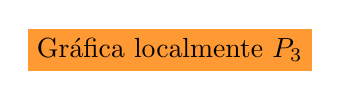
\begin{tikzpicture}
      \grCirculant[RA=2.5]{8}{1,2}
      \uncover<1-3>{\AddVertexColor{red}{a2}}
      \uncover<2,3>{\AddVertexColor{green}{a0,a1,a3,a4}}
      \uncover<3>{%
        \SetUpEdge[lw=5pt,color=blue]
        \Edge(a0)(a1)
        \Edge(a1)(a3)
        \Edge(a3)(a4)
        }
      \uncover<4>{
        \AddVertexColor{red}{a5}
        \AddVertexColor{green}{a3,a4,a6,a7}
        {\SetUpEdge[lw=5pt,color=blue]
          \Edge(a3)(a4)
          \Edge(a6)(a4)
          \Edge(a6)(a7)
        }
      }
      \uncover<5>{
        \AddVertexColor{red}{a0}
        \AddVertexColor{green}{a1,a2,a6,a7}
        {\SetUpEdge[lw=5pt,color=blue]
          \Edge(a1)(a2)
          \Edge(a7)(a1)
          \Edge(a6)(a7)
        }
      }
      \uncover<6>{\draw (0,-3) node [fill=orange!80!white,below]{Gráfica
        localmente $P_{3}$};}
    \end{tikzpicture}
  \end{center} 
\end{standaloneframe}
\end{document}

\end{frame}
\begin{frame}[label=sec-17]{Ejemplo localmente \(P_{4}\)}
\documentclass[beamer]{standalone}

\usetheme{naked}
\setbeamercolor{alerted text}{fg=green!50!black}
\setbeamercolor{box title}{fg=purple}
\setbeamertemplate{frametitle}{}

\usepackage{standalone}

\makeatletter
%\makeatletter

\newcounter{nstart}
\newcounter{nend}

\define@cmdkey[GRA]{small}{i}{}

\newcommand{\graphs}[1]{%
  \setkeys[GRA]{small}{#1}%
  \begin{tikzpicture}[scale=0.4]
  \ifcase\cmdGRA@small@i
  \or % i=1
  \Vertex[x=0,y=0]{a0}
  \or % i=2
  \grEmptyPath[RA=1]{2}
  \or % i=3
  \grPath[RA=1]{2}
  \or % i=4
  \grEmptyPath[RA=1]{3}
  \or % i=5
  \grPath[form=2,rotation=90,RA=1]{2}
  \Vertex[x=1,y=0]{a2}
  \or % i=6
  %\grComplete[RA=1/sqrt(3),rotation=90]{3}
  \grComplete[RA=1/(1+cos(60)),rotation=90]{3}
  \or % i=7
  \grEmptyCycle[RA=1/sqrt(2),rotation=45]{4}
  \or % i=8
  \grPath[form=2,rotation=90,RA=1]{2}
  \grEmptyPath[form=2,x=1,prefix=b,rotation=90,RA=1]{2}
  \or % i=9
  \grPath[form=2,rotation=90,RA=1]{2}
  \grPath[form=2,x=1,prefix=b,rotation=90,RA=1]{2}
  \or % i=10
  \grEmptyCycle[RA=1/sqrt(2),rotation=45]{4}
  \EdgeInGraphLoop{a}{3}
  \or % i=11
  \grEmptyCycle[RA=1/sqrt(2),rotation=45]{4}
  \EdgeInGraphLoop*{a}{4}
  \or % i=12
  \grCycle[RA=1/sqrt(2),rotation=45]{4}
  \or % i=13
  \grComplete[RA=1/sqrt(2),rotation=45]{4}
  \or % i=14
  \grEmptyPath[form=2,RA=1]{3}
  \grEmptyPath[y=1,form=2,RA=1]{2}
  % \grEmptyCycle[RA=1/2*cosec(36),rotation=90]{5}
  \or % i=15
  \grPath[form=2,y=1,RA=1]{2}
  \grEmptyPath[form=2,RA=1]{3}
  \or % i=16
  \grPath[RA=1,form=2,rotation=90]{2}
  \grPath[RA=1,form=2,x=1,y=0,prefix=b,rotation=90]{2}
  \Vertex[x=2,y=0]{c0}
  \or % i=17
  \grPath[RA=1,form=2,rotation=90]{2}
  \grEmptyPath[RA=1,form=2,x=1,y=0,prefix=b,rotation=90]{2}
  \EdgeIdentity{a}{b}{2}
  \Vertex[x=2,y=0]{c0}
  % \grEmptyCycle[RA=1,rotation=90+72]{5}
  % \EdgeInGraphLoop*{a}{4}
  \or % i=18
  \grEmptyPath[RA=1,form=2,rotation=90]{2}
  \grPath[RA=1,form=2,x=1,y=0,prefix=b,rotation=90]{2}
  \Vertex[x=2,y=0]{c0}
  \EdgeFromOneToAll{c}{b}{0}{2}
  % \grEmptyCycle[RA=1,rotation=18]{5}
  % \EdgeInGraphLoop{a}{3}
  \or % i=19
  \grPath[form=2,RA=1]{3}
  \grPath[form=2,RA=1,y=1,prefix=b]{2}
  \or % i=20
  \grPath[RA=1,form=2,rotation=90]{2}
  \grPath[RA=1,form=2,x=1,y=0,prefix=b,rotation=90]{2}
  \EdgeIdentity{a}{b}{2}
  \Vertex[x=2,y=0]{c0}
  % \grEmptyCycle[RA=1,rotation=90+72]{5}
  % \EdgeInGraphLoop{a}{4}
  \or % i=21
  \grEmptyPath[RA=1,form=2,rotation=90]{2}
  \grEmptyPath[RA=1,form=2,x=1,y=0,prefix=b,rotation=90]{2}
  \EdgeIdentity{a}{b}{2}
  \Vertex[x=2,y=0]{c0}
  \EdgeFromOneToAll{c}{b}{0}{2}
  % \grEmptyCycle[RA=1,rotation=-54]{5}
  % \EdgeInGraphLoop*{a}{5}  
  \or % i=22
  \grPath[RA=1,form=2,rotation=90]{2}
  \grPath[RA=1,form=2,x=1,y=0,prefix=b,rotation=90]{2}
  \Vertex[x=2,y=0]{c0}
  \EdgeFromOneToAll{c}{b}{0}{2}
  % \grEmptyCycle[RA=1,rotation=18]{5}
  % \EdgeInGraphLoop{a}{3}
  % \Edge(a3)(a4)
  \or % i=23
  %\grCycle[RA=1/2*cosec(36),rotation=18]{5}
  % \grCycle[RA=1/(1+cos(36)),rotation=18]{5}
  \grPath[form=2,RA=1]{3}
  \grPath[form=2,RA=1,y=1,prefix=b]{2}
  \Edge(a0)(b0)
  \Edge(a2)(b1)
  \or % i=24
  \grPath[RA=1,form=2,rotation=90]{2}
  \grPath[RA=1,form=2,x=2,y=0,prefix=b,rotation=90]{2}
  \Vertex[x=1,y=0]{c0}
  \EdgeFromOneToAll{c}{b}{0}{2}
  \EdgeFromOneToAll{c}{a}{0}{2}
  % \Vertex{a0}
  % \grPath[RA=\edgel,form=2,rotation=90,x=\edgelosqthree,prefix=b]{2}
  % \grPath[RA=\edgel,form=2,rotation=90,x=-\edgelosqthree,prefix=c]{2}
  % \EdgeFromOneToAll{a}{b}{0}{2}
  % \EdgeFromOneToAll{a}{c}{0}{2}
  \or % i=25
  \grPath[RA=1,form=2,rotation=90]{2}
  \grPath[RA=1,form=2,x=1,y=0,prefix=b,rotation=90]{2}
  \EdgeIdentity{a}{b}{2}
  \Edge(a0)(b1)
  \Edge(a1)(b0)
  \Vertex[x=2,y=0]{c0}
  % \grEmptyCycle[RA=1,rotation=90+72]{5}
  % \EdgeInGraphLoop{a}{4}
  % \Edge(a0)(a2)
  % \Edge(a1)(a3)
  \or % i=26
  \grPath[RA=1,form=2,rotation=90]{2}
  \grPath[RA=1,form=2,x=1,y=0,prefix=b,rotation=90]{2}
  \EdgeIdentity{a}{b}{2}
  \Vertex[x=2,y=0]{c0}
  \EdgeFromOneToAll{c}{b}{0}{2}
  % \grCycle[RA=1,rotation=90]{5}
  % \Edge(a1)(a4)
  \or % i=27
  \grComplete[RA=1/2*cosec(36),rotation=90]{5}
  \or % i=28
  \grEmptyPath[form=2,RA=1]{3}
  \grEmptyPath[y=1,form=2,RA=1]{3}
  % \grEmptyCycle[RA=1/2*cosec(30)]{6}
  \or % i=29
  \grEmptyPath[form=2,RA=1]{3}
  \grEmptyPath[y=1,form=2,RA=1,prefix=b]{3}
  \Edge(a0)(b0)
  % \grEmptyCycle[RA=1]{6}
  % \Edge(a4)(a5)
  \or % i=30
  \grEmptyPath[form=2,RA=1]{3}
  \grEmptyPath[y=1,form=2,RA=1,prefix=b]{3}
  \Edge(a0)(b0)
  \Edge(a1)(b1)
  % \grEmptyCycle[RA=1]{6}
  % \Edge(a4)(a5)
  % \Edge(a1)(a2)
  \or % i=31
  \grEmptyPath[form=2,RA=1]{3}
  \grEmptyPath[y=1,form=2,RA=1,prefix=b]{3}
  \Edge(a0)(a1)
  \Edge(a0)(b0)
  \Edge(b0)(b1)
  % \grEmptyCycle[RA=1,rotation=180]{6}
  % \EdgeInGraphLoop*{a}{4}
  \or % i=32
  \grEmptyPath[form=2,RA=1]{3}
  \grEmptyPath[y=1,form=2,RA=1,prefix=b]{3}
  \Edge(a0)(a1)
  \Edge(a0)(b0)
  \Edge(b0)(a1)
  % \grEmptyCycle[RA=1,rotation=-150]{6}
  % \EdgeInGraphLoop{a}{3}
  \or % i=33
  \grEmptyPath[form=2,RA=1]{3}
  \grEmptyPath[y=1,form=2,RA=1,prefix=b]{3}
  \Edge(a0)(a1)
  \Edge(a0)(b0)
  \Edge(b2)(a2)
  % \grEmptyCycle[RA=1,rotation=-150]{6}
  % \EdgeInGraphLoop*{a}{3}
  % \Edge(a3)(a5)
  \or % i=34
  \grEmptyPath[RA=1]{3}
  \grEmptyPath[RA=1,prefix=b,y=1]{3}
  \EdgeIdentity{a}{b}{3}
  \or % i=35
  \grEmptyPath[form=2,RA=1]{3}
  \grEmptyPath[y=1,form=2,RA=1,prefix=b]{3}
  \Edge(a0)(a1)
  \Edge(a0)(b0)
  \Edge(b0)(b1)
  \Edge(a1)(b1)
  % \grEmptyCycle[RA=1,rotation=180]{6}
  % \EdgeInGraphLoop{a}{4}
  \or % i=36
  \grPath[form=2,RA=1]{3}
  \grEmptyPath[y=1,form=2,RA=1,prefix=b]{3}
  \Edge(a0)(b0)
  \Edge(b0)(b1)
  % \grEmptyCycle[RA=1,rotation=150]{6}
  % \EdgeInGraphLoop*{a}{5}
  \or % i=37
  \grEmptyPath[form=2,RA=1]{3}
  \grEmptyPath[y=1,form=2,RA=1,prefix=b]{3}
  \Edge(a0)(a1)
  \Edge(a0)(b0)
  \Edge(a1)(b0)
  \Edge(b2)(a2)
  % \grEmptyCycle[RA=1,rotation=-150]{6}
  % \EdgeInGraphLoop{a}{3}
  % \Edge(a3)(a5)
  \or % i=38
  \grEmptyPath[form=2,RA=1]{3}
  \grEmptyPath[y=1,form=2,RA=1,prefix=b]{3}
  \Edge(a0)(a1)
  \Edge(b0)(b1)
  \Edge(a0)(b0)
  \Edge(b2)(a2)
  % \grEmptyCycle[RA=1,rotation=180]{6}
  % \EdgeInGraphLoop*{a}{4}
  % \Edge(a4)(a5)
  \or % i=39
  \grPath[form=2,RA=1]{3}
  \grEmptyPath[y=1,form=2,RA=1,prefix=b]{3}
  \Edge(a0)(b0)
  \Edge(b0)(b1)
  \Edge(b1)(a2)
  % \grEmptyCycle[RA=1,rotation=150]{6}
  % \EdgeInGraphLoop{a}{5}
  \or % i=40
  \grPath[form=2,RA=1]{3}
  \grPath[y=1,form=2,RA=1,prefix=b]{3}
  \Edge(a0)(b0)
  % \grEmptyCycle[RA=1,rotation=-240]{6}
  % \EdgeInGraphLoop*{a}{6}
  \or % i=41
  \grEmptyPath[form=2,RA=1]{3}
  \grEmptyPath[y=1,form=2,RA=1,prefix=b]{3}
  \Edge(a0)(a1)
  \Edge(b0)(b1)
  \Edge(a1)(b1)
  \Edge(a0)(b0)
  \Edge(b2)(a2)
  % \grEmptyCycle[RA=1,rotation=-180]{6}
  % \EdgeInGraphLoop{a}{4}
  % \Edge(a4)(a5)
  \or % i=42
  \grEmptyPath[RA=1]{3}
  \grEmptyPath[RA=1,prefix=b,y=1]{3}
  \Edge(a0)(b0)
  \Edge(a0)(a1)
  \Edge(a0)(b1)
  \Edge(b0)(b1)
  \Edge(a2)(b2)
  \or % i=43
  \grEmptyPath[form=2,RA=1]{3}
  \grEmptyPath[y=1,form=2,RA=1,prefix=b]{3}
  \Edge(a0)(a1)
  \Edge(b0)(b1)
  \Edge(a1)(b1)
  \Edge(a0)(b0)
  \Edge(a0)(b1)
  \Edge(a1)(b0)
  % \grEmptyCycle[RA=1,rotation=180]{6}
  % \EdgeInGraphLoop{a}{4}
  % \Edge(a0)(a2)
  % \Edge(a1)(a3)
  \or % i=44
  \grPath[form=2,RA=1]{3}
  \grEmptyPath[y=1,form=2,RA=1,prefix=b]{3}
  \Edge(a0)(b0)
  \Edge(b0)(b1)
  \Edge(b1)(a2)
  \Edge(a1)(b1)
  % \grEmptyCycle[RA=1,rotation=150]{6}
  % \EdgeInGraphLoop{a}{5}
  % \Edge(a1)(a3)
  \or % i=45
  \grPath[form=2,RA=1]{3}
  \grEmptyPath[y=1,form=2,RA=1,prefix=b]{3}
  \Edge(a0)(b0)
  \Edge(a1)(b0)
  \Edge(a1)(b2)
  \Edge(b2)(a2)
  % \grEmptyCycle[RA=1,rotation=90]{6}
  % \EdgeInGraphSeq{a}{1}{4}
  % \Edge(a1)(a3)
  % \Edge(a5)(a3)
  \or % i=46
  \grPath[form=2,RA=1]{3}
  \grPath[y=1,form=2,RA=1,prefix=b]{3}
  \Edge(a0)(b0)
  \Edge(a2)(b2)
  % \grCycle[RA=1]{6}
  \or % i=47
  \grPath[form=2,RA=1]{3}
  \grEmptyPath[y=1,form=2,RA=1,prefix=b]{3}
  \Edge(a0)(b0)
  \Edge(a1)(b0)
  \Edge(b2)(a2)
  \Edge(b1)(b2)
  % \grEmptyCycle[RA=1,rotation=30]{6}
  % \EdgeInGraphLoop*{a}{6}
  % \Edge(a0)(a2)
  \or % i=48
  \grPath[RA=1]{3}
  \grPath[RA=1,prefix=b,y=1]{3}
  \EdgeIdentity{a}{b}{2}
  \or % i=49
  \grPath[form=2,RA=1]{3}
  \grPath[y=1,form=2,RA=1,prefix=b]{3}
  \Edge(a0)(b0)
  \Edge(a1)(b0)
  % \grEmptyCycle[RA=1]{6}
  % \EdgeInGraphLoop*{a}{6}
  % \Edge(a1)(a3)
  \or % i=50
  \grPath[form=2,RA=1]{3}
  \grEmptyPath[y=1,form=2,RA=1,prefix=b]{3}
  \Edge(a0)(b0)
  \Edge(a1)(b0)
  \Edge(a1)(b1)
  \Edge(b1)(b2)
  % \grEmptyCycle[RA=1]{6}
  % \EdgeInGraphLoop*{a}{5}
  % \Edge(a2)(a4)  
  % \Edge(a2)(a5)  
  \or % i=51
  \grEmptyPath[form=2,RA=1]{3}
  \grEmptyPath[y=1,form=2,RA=1,prefix=b]{3}
  \Edge(a0)(a1)
  \Edge(a0)(b0)
  \Edge(a1)(b0)
  \Edge(b2)(a2)
  \Edge(b1)(b2)
  \Edge(b1)(a2)
  % \grEmptyCycle[RA=1,rotation=-60]{6}
  % \EdgeInGraphLoop{a}{3}
  % \Edge(a3)(a4)
  % \Edge(a5)(a4)
  % \Edge(a5)(a3)
  \or % i=52
  \grPath[RA=1]{3}
  \grPath[RA=1,prefix=b,y=1]{3}
  \EdgeIdentity{a}{b}{3}
  \or % i=53
  \grPath[form=2,RA=1]{3}
  \grPath[y=1,form=2,RA=1,prefix=b]{3}
  \Edge(a0)(b0)
  \Edge(a2)(b2)
  \Edge(a1)(b0)
  % \grCycle[RA=1]{6}
  % \Edge(a2)(a4)
  \or % i=54
  \grPath[form=2,RA=1]{3}
  \grEmptyPath[y=1,form=2,RA=1,prefix=b]{3}
  \Edge(a1)(b0)
  \Edge(b1)(b2)
  \EdgeIdentity{a}{b}{3}
  % \grEmptyCycle[RA=1,rotation=180]{6}
  % \EdgeInGraphLoop{a}{4}
  % \Edge(a0)(a4)
  % \Edge(a0)(a5)
  % \Edge(a4)(a5)
  \or % i=55
  \grEmptyPath[RA=1]{3}
  \grEmptyPath[RA=1,prefix=b,y=1]{3}
  \EdgeIdentity{a}{b}{3}
  \Edge(a0)(b1)
  \Edge(a0)(a1)
  \Edge(a1)(b0)
  \Edge(b1)(b0)
  \or % i=56
  \grPath[form=2,RA=1]{3}
  \grEmptyPath[y=1,form=2,RA=1,prefix=b]{3}
  \Edge(b1)(b2)
  \Edge(a0)(b0)
  \Edge(a1)(b0)
  \Edge(b2)(a2)
  \Edge(b1)(a2)
  % \grEmptyCycle[RA=1,rotation=-60]{6}
  % \EdgeInGraphLoop{a}{3}
  % \Edge(a3)(a4)
  % \Edge(a5)(a4)
  % \Edge(a5)(a3)
  % \Edge(a5)(a0)
  \or % i=57
  \grPath[form=2,RA=1]{3}
  \grPath[y=1,form=2,RA=1,prefix=b]{3}
  \Edge(a0)(b0)
  \Edge(a1)(b0)
  \Edge(b2)(a2)
  \Edge(b1)(a2)
  % \grCycle[RA=1]{6}
  % \Edge(a1)(a5)
  % \Edge(a2)(a4)
  \or % i=58
  \grPath[form=2,RA=1]{3}
  \grPath[y=1,form=2,RA=1,prefix=b]{3}
  \Edge(a0)(b0)
  \Edge(a1)(b0)
  \Edge(b2)(a2)
  \Edge(b1)(a2)
  \Edge(a0)(b2)
  % \grCycle[RA=1]{6}
  % \Edge(a1)(a5)
  % \Edge(a2)(a4)
  % \Edge(a0)(a3)
  \or % i=59
  \grPath[form=2,RA=1]{3}
  \grPath[y=1,form=2,RA=1,prefix=b]{3}
  \EdgeIdentity{a}{b}{3}
  \Edge(a1)(b0)
  \Edge(b1)(a2)
  % \grCycle[RA=1]{6}
  % \Edge(a1)(a5)
  % \Edge(a2)(a4)
  % \Edge(a1)(a4)
  \or % i=60
  \grPath[RA=1]{3}
  \grPath[RA=1,prefix=b,y=1]{3}
  \EdgeIdentity{a}{b}{3}
  \Edge(a0)(b1)
  \Edge(b0)(a1)
  \or % i=61
  \grCompleteBipartite[RA=1,RB=1,RS=1]{3}{3}
  \or % i=62
  \grCycle[RA=1]{6}
  \Edge(a1)(a5)
  \Edge(a2)(a4)
  \Edge(a3)(a5)
  \Edge(a0)(a4)
  \or % i=63
  \grComplete[RA=1/2*cosec(36),rotation=90]{5}
  \Vertex[x=1.5,y=0]{b0}
  % \grEmptyCycle[RA=1,rotation=150]{6}
  % \EdgeInGraphLoop{a}{5}
  % \Edge(a0)(a2)
  % \Edge(a0)(a3)
  % \Edge(a1)(a3)
  % \Edge(a1)(a4)
  % \Edge(a2)(a4)
  \or % i=64
  \grCirculant[RA=1]{6}{1,2}
  \or % i=65
  \grComplete[RA=1]{6}
  \fi
  \end{tikzpicture}
}

\newcommand{\names}[1]{%
  \setkeys[GRA]{small}{#1}%
  \ifcase\cmdGRA@small@i
  \or % i=1
  $K_{1}$
  \or % i=2
  $2K_{1}$
  \or % i=3
  $K_{2}$
  \or % i=4
  $3K_{1}$
  \or % i=5
  $K_{2}\cup K_{1}$
  \or % i=6
  $K_{3}$
  \or % i=7
  $4K_{1}$
  \or % i=8
  $K_{2}\cup 2K_{1}$
  \or % i=9
  $2K_{2}$
  \or % i=10
  $K_{3}\cup K_{1}$
  \or % i=11
  $P_{3}$
  \or % i=12
  $C_{4}$
  \or % i=13
  $K_{4}$
  \or % i=14
  $5K_{1}$
  \or % i=15
  $K_{2}\cup 3K_{1}$
  \or % i=16
  $2K_{2}\cup K_{1}$
  \or % i=17
  $P_{3}\cup K_{1}$
  \or % i=18
  $K_{3}\cup 2K_{1}$
  \or % i=19
  $P_{2}\cup K_{2}$
  \or % i=20
  $C_{4}\cup K_{1}$
  \or % i=21
  $P_{4}$
  \or % i=22
  $K_{3}\cup K_{2}$
  \or % i=23
  $C_{5}$
  \or % i=24
  \fbox{$(5,6,1)$}
  \or % i=25
  $K_{4}\cup K_{1}$
  \or % i=26
  \fbox{$(5,6,4)$}
  \or % i=27
  $K_{5}$
  \or % i=28
  $6K_{1}$
  \or % i=29
  $K_{2}\cup 4K_{1}$
  \or % i=30
  $2K_{2}\cup 2K_{1}$
  \or % i=31
  $P_{3}\cup 2K_{1}$
  \or % i=32
  $K_{3}\cup 3K_{1}$
  \or % i=33
  $P_{2}\cup K_{2}\cup K_{1}$
  \or % i=34
  $3K_{2}$
  \or % i=35
  $C_{4}\cup 2K_{1}$
  \or % i=36
  $P_{4}\cup K_{1}$
  \or % i=37
  $K_{3}\cup K_{2}\cup K_{1}$
  \or % i=38
  $P_{3}\cup K_{2}$
  \or % i=39
  $C_{5}\cup K_{1}$
  \or % i=40
  $P_{5}$
  \or % i=41
  $C_{4}\cup K_{2}$
  \or % i=42
  \fbox{$(6,5,15)$}
  \or % i=43
  $K_{4}\cup 2K_{1}$
  \or % i=44
  \fbox{$(6,6,2)$}
  \or % i=45
  \fbox{$(6,6,3)$}
  \or % i=46
  $C_{6}$
  \or % i=47
  \fbox{$(6,6,10)$}
  \or % i=48
  \fbox{$(6,6,11)$}
  \or % i=49
  \fbox{$(6,6,13)$}
  \or % i=50
  \fbox{$(6,6,14)$}
  \or % i=51
  $2K_{3}$
  \or % i=52
  \fbox{$(6,7,5)$}
  \or % i=53
  \fbox{$(6,7,6)$}
  \or % i=54
  \fbox{$(6,7,13)$}
  \or % i=55
  $K_{4}\cup K_{2}$
  \or % i=56
  \fbox{$(6,7,23)$}
  \or % i=57
  \fbox{$(6,8,5)$}
  \or % i=58
  \fbox{$(6,9,7)$}
  \or % i=59
  \fbox{$(6,9,11)$}
  \or % i=60
  \fbox{$(6,9,16)$}
  \or % i=61
  $K_{3,3}$
  \or % i=62
  \fbox{$(6,10,7)$}
  \or % i=63
  $K_{5}\cup K_{1}$
  \or % i=64
  $O_{3}$
  \or % i=65
  $K_{6}$
  \fi
}
%\makeatother

\newcommand{\graphst}[2]{%
  \setkeys[GRA]{small}{#1}%
  \begin{tikzpicture}[scale=#2]
  \ifcase\cmdGRA@small@i
  \or % i=1
  \Vertex[x=0,y=0]{a0}
  \or % i=2
  \grEmptyPath[RA=1]{2}
  \or % i=3
  \grPath[RA=1]{2}
  \or % i=4
  \grEmptyPath[RA=1]{3}
  \or % i=5
  \grPath[form=2,rotation=90,RA=1]{2}
  \Vertex[x=1,y=0]{a2}
  \or % i=6
  \grComplete[RA=1/(1+cos(60)),rotation=90]{3}
  \or % i=7
  \grEmptyCycle[RA=1/sqrt(2),rotation=45]{4}
  \or % i=8
  \grPath[form=2,rotation=90,RA=1]{2}
  \grEmptyPath[form=2,x=1,prefix=b,rotation=90,RA=1]{2}
  \or % i=9
  \grPath[form=2,rotation=90,RA=1]{2}
  \grPath[form=2,x=1,prefix=b,rotation=90,RA=1]{2}
  \or % i=10
  \grEmptyCycle[RA=1/sqrt(2),rotation=45]{4}
  \EdgeInGraphLoop{a}{3}
  \or % i=11
  \grEmptyCycle[RA=1/sqrt(2),rotation=45]{4}
  \EdgeInGraphLoop*{a}{4}
  \or % i=12
  \grCycle[RA=1/sqrt(2),rotation=45]{4}
  \or % i=13
  \grComplete[RA=1/sqrt(2),rotation=45]{4}
  \or % i=14
  \grEmptyPath[form=2,RA=1]{3}
  \grEmptyPath[y=1,form=2,RA=1]{2}
  \or % i=15
  \grPath[form=2,y=1,RA=1]{2}
  \grEmptyPath[form=2,RA=1]{3}
  \or % i=16
  \grPath[RA=1,form=2,rotation=90]{2}
  \grPath[RA=1,form=2,x=1,y=0,prefix=b,rotation=90]{2}
  \Vertex[x=2,y=0]{c0}
  \or % i=17
  \grPath[RA=1,form=2,rotation=90]{2}
  \grEmptyPath[RA=1,form=2,x=1,y=0,prefix=b,rotation=90]{2}
  \EdgeIdentity{a}{b}{2}
  \Vertex[x=2,y=0]{c0}
  \or % i=18
  \grEmptyPath[RA=1,form=2,rotation=90]{2}
  \grPath[RA=1,form=2,x=1,y=0,prefix=b,rotation=90]{2}
  \Vertex[x=2,y=0]{c0}
  \EdgeFromOneToAll{c}{b}{0}{2}
  \or % i=19
  \grPath[form=2,RA=1]{3}
  \grPath[form=2,RA=1,y=1,prefix=b]{2}
  \or % i=20
  \grPath[RA=1,form=2,rotation=90]{2}
  \grPath[RA=1,form=2,x=1,y=0,prefix=b,rotation=90]{2}
  \EdgeIdentity{a}{b}{2}
  \Vertex[x=2,y=0]{c0}
  \or % i=21
  \grEmptyPath[RA=1,form=2,rotation=90]{2}
  \grEmptyPath[RA=1,form=2,x=1,y=0,prefix=b,rotation=90]{2}
  \EdgeIdentity{a}{b}{2}
  \Vertex[x=2,y=0]{c0}
  \EdgeFromOneToAll{c}{b}{0}{2}
  \or % i=22
  \grPath[RA=1,form=2,rotation=90]{2}
  \grPath[RA=1,form=2,x=1,y=0,prefix=b,rotation=90]{2}
  \Vertex[x=2,y=0]{c0}
  \EdgeFromOneToAll{c}{b}{0}{2}
  \or % i=23
  \grPath[form=2,RA=1]{3}
  \grPath[form=2,RA=1,y=1,prefix=b]{2}
  \Edge(a0)(b0)
  \Edge(a2)(b1)
  \or % i=24
  \grPath[RA=1,form=2,rotation=90]{2}
  \grPath[RA=1,form=2,x=2,y=0,prefix=b,rotation=90]{2}
  \Vertex[x=1,y=0]{c0}
  \EdgeFromOneToAll{c}{b}{0}{2}
  \EdgeFromOneToAll{c}{a}{0}{2}
  \or % i=25
  \grPath[RA=1,form=2,rotation=90]{2}
  \grPath[RA=1,form=2,x=1,y=0,prefix=b,rotation=90]{2}
  \EdgeIdentity{a}{b}{2}
  \Edge(a0)(b1)
  \Edge(a1)(b0)
  \Vertex[x=2,y=0]{c0}
  \or % i=26
  \grPath[RA=1,form=2,rotation=90]{2}
  \grPath[RA=1,form=2,x=1,y=0,prefix=b,rotation=90]{2}
  \EdgeIdentity{a}{b}{2}
  \Vertex[x=2,y=0]{c0}
  \EdgeFromOneToAll{c}{b}{0}{2}
  \or % i=27
  \grComplete[RA=1/2*cosec(36),rotation=90]{5}
  \or % i=28
  \grEmptyPath[form=2,RA=1]{3}
  \grEmptyPath[y=1,form=2,RA=1]{3}
  \or % i=29
  \grEmptyPath[form=2,RA=1]{3}
  \grEmptyPath[y=1,form=2,RA=1,prefix=b]{3}
  \Edge(a0)(b0)
  \or % i=30
  \grEmptyPath[form=2,RA=1]{3}
  \grEmptyPath[y=1,form=2,RA=1,prefix=b]{3}
  \Edge(a0)(b0)
  \Edge(a1)(b1)
  \or % i=31
  \grEmptyPath[form=2,RA=1]{3}
  \grEmptyPath[y=1,form=2,RA=1,prefix=b]{3}
  \Edge(a0)(a1)
  \Edge(a0)(b0)
  \Edge(b0)(b1)
  \or % i=32
  \grEmptyPath[form=2,RA=1]{3}
  \grEmptyPath[y=1,form=2,RA=1,prefix=b]{3}
  \Edge(a0)(a1)
  \Edge(a0)(b0)
  \Edge(b0)(a1)
  \or % i=33
  \grEmptyPath[form=2,RA=1]{3}
  \grEmptyPath[y=1,form=2,RA=1,prefix=b]{3}
  \Edge(a0)(a1)
  \Edge(a0)(b0)
  \Edge(b2)(a2)
  \or % i=34
  \grEmptyPath[RA=1]{3}
  \grEmptyPath[RA=1,prefix=b,y=1]{3}
  \EdgeIdentity{a}{b}{3}
  \or % i=35
  \grEmptyPath[form=2,RA=1]{3}
  \grEmptyPath[y=1,form=2,RA=1,prefix=b]{3}
  \Edge(a0)(a1)
  \Edge(a0)(b0)
  \Edge(b0)(b1)
  \Edge(a1)(b1)
  \or % i=36
  \grPath[form=2,RA=1]{3}
  \grEmptyPath[y=1,form=2,RA=1,prefix=b]{3}
  \Edge(a0)(b0)
  \Edge(b0)(b1)
  \or % i=37
  \grEmptyPath[form=2,RA=1]{3}
  \grEmptyPath[y=1,form=2,RA=1,prefix=b]{3}
  \Edge(a0)(a1)
  \Edge(a0)(b0)
  \Edge(a1)(b0)
  \Edge(b2)(a2)
  \or % i=38
  \grEmptyPath[form=2,RA=1]{3}
  \grEmptyPath[y=1,form=2,RA=1,prefix=b]{3}
  \Edge(a0)(a1)
  \Edge(b0)(b1)
  \Edge(a0)(b0)
  \Edge(b2)(a2)
  \or % i=39
  \grPath[form=2,RA=1]{3}
  \grEmptyPath[y=1,form=2,RA=1,prefix=b]{3}
  \Edge(a0)(b0)
  \Edge(b0)(b1)
  \Edge(b1)(a2)
  \or % i=40
  \grPath[form=2,RA=1]{3}
  \grPath[y=1,form=2,RA=1,prefix=b]{3}
  \Edge(a0)(b0)
  \or % i=41
  \grEmptyPath[form=2,RA=1]{3}
  \grEmptyPath[y=1,form=2,RA=1,prefix=b]{3}
  \Edge(a0)(a1)
  \Edge(b0)(b1)
  \Edge(a1)(b1)
  \Edge(a0)(b0)
  \Edge(b2)(a2)
  \or % i=42
  \grEmptyPath[RA=1]{3}
  \grEmptyPath[RA=1,prefix=b,y=1]{3}
  \Edge(a0)(b0)
  \Edge(a0)(a1)
  \Edge(a0)(b1)
  \Edge(b0)(b1)
  \Edge(a2)(b2)
  \or % i=43
  \grEmptyPath[form=2,RA=1]{3}
  \grEmptyPath[y=1,form=2,RA=1,prefix=b]{3}
  \Edge(a0)(a1)
  \Edge(b0)(b1)
  \Edge(a1)(b1)
  \Edge(a0)(b0)
  \Edge(a0)(b1)
  \Edge(a1)(b0)
  \or % i=44
  \grPath[form=2,RA=1]{3}
  \grEmptyPath[y=1,form=2,RA=1,prefix=b]{3}
  \Edge(a0)(b0)
  \Edge(b0)(b1)
  \Edge(b1)(a2)
  \Edge(a1)(b1)
  \or % i=45
  \grPath[form=2,RA=1]{3}
  \grEmptyPath[y=1,form=2,RA=1,prefix=b]{3}
  \Edge(a0)(b0)
  \Edge(a1)(b0)
  \Edge(a1)(b2)
  \Edge(b2)(a2)
  \or % i=46
  \grPath[form=2,RA=1]{3}
  \grPath[y=1,form=2,RA=1,prefix=b]{3}
  \Edge(a0)(b0)
  \Edge(a2)(b2)
  \or % i=47
  \grPath[form=2,RA=1]{3}
  \grEmptyPath[y=1,form=2,RA=1,prefix=b]{3}
  \Edge(a0)(b0)
  \Edge(a1)(b0)
  \Edge(b2)(a2)
  \Edge(b1)(b2)
  \or % i=48
  \grPath[RA=1]{3}
  \grPath[RA=1,prefix=b,y=1]{3}
  \EdgeIdentity{a}{b}{2}
  \or % i=49
  \grPath[form=2,RA=1]{3}
  \grPath[y=1,form=2,RA=1,prefix=b]{3}
  \Edge(a0)(b0)
  \Edge(a1)(b0)
  \or % i=50
  \grPath[form=2,RA=1]{3}
  \grEmptyPath[y=1,form=2,RA=1,prefix=b]{3}
  \Edge(a0)(b0)
  \Edge(a1)(b0)
  \Edge(a1)(b1)
  \Edge(b1)(b2)
  \or % i=51
  \grEmptyPath[form=2,RA=1]{3}
  \grEmptyPath[y=1,form=2,RA=1,prefix=b]{3}
  \Edge(a0)(a1)
  \Edge(a0)(b0)
  \Edge(a1)(b0)
  \Edge(b2)(a2)
  \Edge(b1)(b2)
  \Edge(b1)(a2)
  \or % i=52
  \grPath[RA=1]{3}
  \grPath[RA=1,prefix=b,y=1]{3}
  \EdgeIdentity{a}{b}{3}
  \or % i=53
  \grPath[form=2,RA=1]{3}
  \grPath[y=1,form=2,RA=1,prefix=b]{3}
  \Edge(a0)(b0)
  \Edge(a2)(b2)
  \Edge(a1)(b0)
  \or % i=54
  \grPath[form=2,RA=1]{3}
  \grEmptyPath[y=1,form=2,RA=1,prefix=b]{3}
  \Edge(a1)(b0)
  \Edge(b1)(b2)
  \EdgeIdentity{a}{b}{3}
  \or % i=55
  \grEmptyPath[RA=1]{3}
  \grEmptyPath[RA=1,prefix=b,y=1]{3}
  \EdgeIdentity{a}{b}{3}
  \Edge(a0)(b1)
  \Edge(a0)(a1)
  \Edge(a1)(b0)
  \Edge(b1)(b0)
  \or % i=56
  \grPath[form=2,RA=1]{3}
  \grEmptyPath[y=1,form=2,RA=1,prefix=b]{3}
  \Edge(b1)(b2)
  \Edge(a0)(b0)
  \Edge(a1)(b0)
  \Edge(b2)(a2)
  \Edge(b1)(a2)
  \or % i=57
  \grPath[form=2,RA=1]{3}
  \grPath[y=1,form=2,RA=1,prefix=b]{3}
  \Edge(a0)(b0)
  \Edge(a1)(b0)
  \Edge(b2)(a2)
  \Edge(b1)(a2)
  \or % i=58
  \grPath[form=2,RA=1]{3}
  \grPath[y=1,form=2,RA=1,prefix=b]{3}
  \Edge(a0)(b0)
  \Edge(a1)(b0)
  \Edge(b2)(a2)
  \Edge(b1)(a2)
  \Edge(a0)(b2)
  \or % i=59
  \grPath[form=2,RA=1]{3}
  \grPath[y=1,form=2,RA=1,prefix=b]{3}
  \EdgeIdentity{a}{b}{3}
  \Edge(a1)(b0)
  \Edge(b1)(a2)
  \or % i=60
  \grPath[RA=1]{3}
  \grPath[RA=1,prefix=b,y=1]{3}
  \EdgeIdentity{a}{b}{3}
  \Edge(a0)(b1)
  \Edge(b0)(a1)
  \or % i=61
  \grCompleteBipartite[RA=1,RB=1,RS=1]{3}{3}
  \or % i=62
  \grCycle[RA=1]{6}
  \Edge(a1)(a5)
  \Edge(a2)(a4)
  \Edge(a3)(a5)
  \Edge(a0)(a4)
  \or % i=63
  \grComplete[RA=1/2*cosec(36),rotation=90]{5}
  \Vertex[x=1.5,y=0]{b0}
  \or % i=64
  \grCirculant[RA=1]{6}{1,2}
  \or % i=65
  \grComplete[RA=1]{6}
  \fi
  \end{tikzpicture}
}

\makeatother

% vertical centering of cells
% see http://tex.stackexchange.com/questions/46386/vertically-center-cells-of-a-table
\usepackage{array}% http://ctan.org/pkg/array
\newcolumntype{M}{>{\centering\arraybackslash}m{\dimexpr.17\linewidth-2\tabcolsep}}

% remove space between margin and lists
\usepackage{enumitem}
\setitemize{label=\usebeamerfont*{itemize item}%
  \usebeamercolor[fg]{itemize item}
  \usebeamertemplate{itemize item}}
\setlist{leftmargin=*,labelindent=0cm}

\usepackage{tikz}
\usepackage{tkz-graph}
\usepackage{tkz-berge}
\usepackage{tkz-berge-add}

\usepackage[utf8]{inputenc}

\usepackage[math]{iwona}

\newcommand{\graphcaption}[4][gray!80!white]{\draw (#2,#3) node [fill=#1]{#4};}

\SetVertexSimple[FillColor=gray, MinSize=7pt, LineWidth=1pt]

\tikzset{EdgeStyle/.style= {%
    color           = white,
    double          = black,
    double distance = 1pt}}

\newcommand{\setof}[2]{\left\{\,#1\mid #2\,\right\}}

\newcommand{\triangulo}[4]{%
  \shadedraw[inner color=#4,opacity=0.8,line width=1pt]
  (#1.center) -- (#2.center) -- (#3.center) -- cycle;}


\begin{document}
\begin{standaloneframe}
  \begin{center}
    \begin{tikzpicture}[scale=0.8]
      \grCycle[RA=1,prefix=a]{4}
      \grEmptyCycle[RA=2,prefix=b]{4}
      \grEmptyCycle[RA=3,prefix=d]{4}
      \begin{scope}[rotate=45]
        \grEmptyCycle[RA=2,prefix=c]{4}
        \grEmptyCycle[RA=3,prefix=e]{4}
        \grCycle[RA=5,prefix=f]{4}
      \end{scope}
      \EdgeIdentity{b}{a}{4}
      \EdgeIdentity{b}{c}{4}
      \EdgeIdentity{b}{e}{4}
      \EdgeIdentity{a}{c}{4}
      \EdgeIdentity{b}{d}{4}
      \EdgeIdentity{d}{e}{4}
      \EdgeIdentity{c}{e}{4}
      \EdgeIdentity{d}{f}{4}
      \EdgeIdentity{e}{f}{4}
      \EdgeMod{c}{b}{4}{1}
      \EdgeMod{e}{d}{4}{1}
      \EdgeMod{f}{d}{4}{1}
      \EdgeMod{a}{c}{4}{3}
      \uncover<2-4>{\AddVertexColor{red}{a0}}
      \uncover<3-4>{\AddVertexColor{orange}{a3,c3,b0,c0,a1}}
      \uncover<4>{{%
          \SetUpEdge[lw=5pt,color=blue]
          \Edge(a3)(c3)
          \Edge(b0)(c3)
          \Edge(b0)(c0)
          \Edge(c0)(a1)
        }}
      \uncover<5-7>{\AddVertexColor{red}{d2}}
      \uncover<6-7>{\AddVertexColor{orange}{b2,e2,f2,f1,e1}}
      \uncover<7>{{%
          \SetUpEdge[lw=5pt,color=blue]
          \Edge(b2)(e2)
          \Edge(e2)(f2)
          \Edge(f2)(f1)
          \Edge(f1)(e1)
          }}
      \uncover<8>{\draw (0,-4) node [fill=orange!80!white,below]{Gráfica
        localmente $P_{4}$};}
    \end{tikzpicture}
  \end{center}  
\end{standaloneframe}
\end{document}

\end{frame}
\begin{frame}[label=sec-18]{Teorema}
\documentclass[beamer]{standalone}

\usetheme{naked}
\setbeamercolor{alerted text}{fg=green!50!black}
\setbeamercolor{box title}{fg=purple}
\setbeamertemplate{frametitle}{}

\usepackage{standalone}

\makeatletter
%\makeatletter

\newcounter{nstart}
\newcounter{nend}

\define@cmdkey[GRA]{small}{i}{}

\newcommand{\graphs}[1]{%
  \setkeys[GRA]{small}{#1}%
  \begin{tikzpicture}[scale=0.4]
  \ifcase\cmdGRA@small@i
  \or % i=1
  \Vertex[x=0,y=0]{a0}
  \or % i=2
  \grEmptyPath[RA=1]{2}
  \or % i=3
  \grPath[RA=1]{2}
  \or % i=4
  \grEmptyPath[RA=1]{3}
  \or % i=5
  \grPath[form=2,rotation=90,RA=1]{2}
  \Vertex[x=1,y=0]{a2}
  \or % i=6
  %\grComplete[RA=1/sqrt(3),rotation=90]{3}
  \grComplete[RA=1/(1+cos(60)),rotation=90]{3}
  \or % i=7
  \grEmptyCycle[RA=1/sqrt(2),rotation=45]{4}
  \or % i=8
  \grPath[form=2,rotation=90,RA=1]{2}
  \grEmptyPath[form=2,x=1,prefix=b,rotation=90,RA=1]{2}
  \or % i=9
  \grPath[form=2,rotation=90,RA=1]{2}
  \grPath[form=2,x=1,prefix=b,rotation=90,RA=1]{2}
  \or % i=10
  \grEmptyCycle[RA=1/sqrt(2),rotation=45]{4}
  \EdgeInGraphLoop{a}{3}
  \or % i=11
  \grEmptyCycle[RA=1/sqrt(2),rotation=45]{4}
  \EdgeInGraphLoop*{a}{4}
  \or % i=12
  \grCycle[RA=1/sqrt(2),rotation=45]{4}
  \or % i=13
  \grComplete[RA=1/sqrt(2),rotation=45]{4}
  \or % i=14
  \grEmptyPath[form=2,RA=1]{3}
  \grEmptyPath[y=1,form=2,RA=1]{2}
  % \grEmptyCycle[RA=1/2*cosec(36),rotation=90]{5}
  \or % i=15
  \grPath[form=2,y=1,RA=1]{2}
  \grEmptyPath[form=2,RA=1]{3}
  \or % i=16
  \grPath[RA=1,form=2,rotation=90]{2}
  \grPath[RA=1,form=2,x=1,y=0,prefix=b,rotation=90]{2}
  \Vertex[x=2,y=0]{c0}
  \or % i=17
  \grPath[RA=1,form=2,rotation=90]{2}
  \grEmptyPath[RA=1,form=2,x=1,y=0,prefix=b,rotation=90]{2}
  \EdgeIdentity{a}{b}{2}
  \Vertex[x=2,y=0]{c0}
  % \grEmptyCycle[RA=1,rotation=90+72]{5}
  % \EdgeInGraphLoop*{a}{4}
  \or % i=18
  \grEmptyPath[RA=1,form=2,rotation=90]{2}
  \grPath[RA=1,form=2,x=1,y=0,prefix=b,rotation=90]{2}
  \Vertex[x=2,y=0]{c0}
  \EdgeFromOneToAll{c}{b}{0}{2}
  % \grEmptyCycle[RA=1,rotation=18]{5}
  % \EdgeInGraphLoop{a}{3}
  \or % i=19
  \grPath[form=2,RA=1]{3}
  \grPath[form=2,RA=1,y=1,prefix=b]{2}
  \or % i=20
  \grPath[RA=1,form=2,rotation=90]{2}
  \grPath[RA=1,form=2,x=1,y=0,prefix=b,rotation=90]{2}
  \EdgeIdentity{a}{b}{2}
  \Vertex[x=2,y=0]{c0}
  % \grEmptyCycle[RA=1,rotation=90+72]{5}
  % \EdgeInGraphLoop{a}{4}
  \or % i=21
  \grEmptyPath[RA=1,form=2,rotation=90]{2}
  \grEmptyPath[RA=1,form=2,x=1,y=0,prefix=b,rotation=90]{2}
  \EdgeIdentity{a}{b}{2}
  \Vertex[x=2,y=0]{c0}
  \EdgeFromOneToAll{c}{b}{0}{2}
  % \grEmptyCycle[RA=1,rotation=-54]{5}
  % \EdgeInGraphLoop*{a}{5}  
  \or % i=22
  \grPath[RA=1,form=2,rotation=90]{2}
  \grPath[RA=1,form=2,x=1,y=0,prefix=b,rotation=90]{2}
  \Vertex[x=2,y=0]{c0}
  \EdgeFromOneToAll{c}{b}{0}{2}
  % \grEmptyCycle[RA=1,rotation=18]{5}
  % \EdgeInGraphLoop{a}{3}
  % \Edge(a3)(a4)
  \or % i=23
  %\grCycle[RA=1/2*cosec(36),rotation=18]{5}
  % \grCycle[RA=1/(1+cos(36)),rotation=18]{5}
  \grPath[form=2,RA=1]{3}
  \grPath[form=2,RA=1,y=1,prefix=b]{2}
  \Edge(a0)(b0)
  \Edge(a2)(b1)
  \or % i=24
  \grPath[RA=1,form=2,rotation=90]{2}
  \grPath[RA=1,form=2,x=2,y=0,prefix=b,rotation=90]{2}
  \Vertex[x=1,y=0]{c0}
  \EdgeFromOneToAll{c}{b}{0}{2}
  \EdgeFromOneToAll{c}{a}{0}{2}
  % \Vertex{a0}
  % \grPath[RA=\edgel,form=2,rotation=90,x=\edgelosqthree,prefix=b]{2}
  % \grPath[RA=\edgel,form=2,rotation=90,x=-\edgelosqthree,prefix=c]{2}
  % \EdgeFromOneToAll{a}{b}{0}{2}
  % \EdgeFromOneToAll{a}{c}{0}{2}
  \or % i=25
  \grPath[RA=1,form=2,rotation=90]{2}
  \grPath[RA=1,form=2,x=1,y=0,prefix=b,rotation=90]{2}
  \EdgeIdentity{a}{b}{2}
  \Edge(a0)(b1)
  \Edge(a1)(b0)
  \Vertex[x=2,y=0]{c0}
  % \grEmptyCycle[RA=1,rotation=90+72]{5}
  % \EdgeInGraphLoop{a}{4}
  % \Edge(a0)(a2)
  % \Edge(a1)(a3)
  \or % i=26
  \grPath[RA=1,form=2,rotation=90]{2}
  \grPath[RA=1,form=2,x=1,y=0,prefix=b,rotation=90]{2}
  \EdgeIdentity{a}{b}{2}
  \Vertex[x=2,y=0]{c0}
  \EdgeFromOneToAll{c}{b}{0}{2}
  % \grCycle[RA=1,rotation=90]{5}
  % \Edge(a1)(a4)
  \or % i=27
  \grComplete[RA=1/2*cosec(36),rotation=90]{5}
  \or % i=28
  \grEmptyPath[form=2,RA=1]{3}
  \grEmptyPath[y=1,form=2,RA=1]{3}
  % \grEmptyCycle[RA=1/2*cosec(30)]{6}
  \or % i=29
  \grEmptyPath[form=2,RA=1]{3}
  \grEmptyPath[y=1,form=2,RA=1,prefix=b]{3}
  \Edge(a0)(b0)
  % \grEmptyCycle[RA=1]{6}
  % \Edge(a4)(a5)
  \or % i=30
  \grEmptyPath[form=2,RA=1]{3}
  \grEmptyPath[y=1,form=2,RA=1,prefix=b]{3}
  \Edge(a0)(b0)
  \Edge(a1)(b1)
  % \grEmptyCycle[RA=1]{6}
  % \Edge(a4)(a5)
  % \Edge(a1)(a2)
  \or % i=31
  \grEmptyPath[form=2,RA=1]{3}
  \grEmptyPath[y=1,form=2,RA=1,prefix=b]{3}
  \Edge(a0)(a1)
  \Edge(a0)(b0)
  \Edge(b0)(b1)
  % \grEmptyCycle[RA=1,rotation=180]{6}
  % \EdgeInGraphLoop*{a}{4}
  \or % i=32
  \grEmptyPath[form=2,RA=1]{3}
  \grEmptyPath[y=1,form=2,RA=1,prefix=b]{3}
  \Edge(a0)(a1)
  \Edge(a0)(b0)
  \Edge(b0)(a1)
  % \grEmptyCycle[RA=1,rotation=-150]{6}
  % \EdgeInGraphLoop{a}{3}
  \or % i=33
  \grEmptyPath[form=2,RA=1]{3}
  \grEmptyPath[y=1,form=2,RA=1,prefix=b]{3}
  \Edge(a0)(a1)
  \Edge(a0)(b0)
  \Edge(b2)(a2)
  % \grEmptyCycle[RA=1,rotation=-150]{6}
  % \EdgeInGraphLoop*{a}{3}
  % \Edge(a3)(a5)
  \or % i=34
  \grEmptyPath[RA=1]{3}
  \grEmptyPath[RA=1,prefix=b,y=1]{3}
  \EdgeIdentity{a}{b}{3}
  \or % i=35
  \grEmptyPath[form=2,RA=1]{3}
  \grEmptyPath[y=1,form=2,RA=1,prefix=b]{3}
  \Edge(a0)(a1)
  \Edge(a0)(b0)
  \Edge(b0)(b1)
  \Edge(a1)(b1)
  % \grEmptyCycle[RA=1,rotation=180]{6}
  % \EdgeInGraphLoop{a}{4}
  \or % i=36
  \grPath[form=2,RA=1]{3}
  \grEmptyPath[y=1,form=2,RA=1,prefix=b]{3}
  \Edge(a0)(b0)
  \Edge(b0)(b1)
  % \grEmptyCycle[RA=1,rotation=150]{6}
  % \EdgeInGraphLoop*{a}{5}
  \or % i=37
  \grEmptyPath[form=2,RA=1]{3}
  \grEmptyPath[y=1,form=2,RA=1,prefix=b]{3}
  \Edge(a0)(a1)
  \Edge(a0)(b0)
  \Edge(a1)(b0)
  \Edge(b2)(a2)
  % \grEmptyCycle[RA=1,rotation=-150]{6}
  % \EdgeInGraphLoop{a}{3}
  % \Edge(a3)(a5)
  \or % i=38
  \grEmptyPath[form=2,RA=1]{3}
  \grEmptyPath[y=1,form=2,RA=1,prefix=b]{3}
  \Edge(a0)(a1)
  \Edge(b0)(b1)
  \Edge(a0)(b0)
  \Edge(b2)(a2)
  % \grEmptyCycle[RA=1,rotation=180]{6}
  % \EdgeInGraphLoop*{a}{4}
  % \Edge(a4)(a5)
  \or % i=39
  \grPath[form=2,RA=1]{3}
  \grEmptyPath[y=1,form=2,RA=1,prefix=b]{3}
  \Edge(a0)(b0)
  \Edge(b0)(b1)
  \Edge(b1)(a2)
  % \grEmptyCycle[RA=1,rotation=150]{6}
  % \EdgeInGraphLoop{a}{5}
  \or % i=40
  \grPath[form=2,RA=1]{3}
  \grPath[y=1,form=2,RA=1,prefix=b]{3}
  \Edge(a0)(b0)
  % \grEmptyCycle[RA=1,rotation=-240]{6}
  % \EdgeInGraphLoop*{a}{6}
  \or % i=41
  \grEmptyPath[form=2,RA=1]{3}
  \grEmptyPath[y=1,form=2,RA=1,prefix=b]{3}
  \Edge(a0)(a1)
  \Edge(b0)(b1)
  \Edge(a1)(b1)
  \Edge(a0)(b0)
  \Edge(b2)(a2)
  % \grEmptyCycle[RA=1,rotation=-180]{6}
  % \EdgeInGraphLoop{a}{4}
  % \Edge(a4)(a5)
  \or % i=42
  \grEmptyPath[RA=1]{3}
  \grEmptyPath[RA=1,prefix=b,y=1]{3}
  \Edge(a0)(b0)
  \Edge(a0)(a1)
  \Edge(a0)(b1)
  \Edge(b0)(b1)
  \Edge(a2)(b2)
  \or % i=43
  \grEmptyPath[form=2,RA=1]{3}
  \grEmptyPath[y=1,form=2,RA=1,prefix=b]{3}
  \Edge(a0)(a1)
  \Edge(b0)(b1)
  \Edge(a1)(b1)
  \Edge(a0)(b0)
  \Edge(a0)(b1)
  \Edge(a1)(b0)
  % \grEmptyCycle[RA=1,rotation=180]{6}
  % \EdgeInGraphLoop{a}{4}
  % \Edge(a0)(a2)
  % \Edge(a1)(a3)
  \or % i=44
  \grPath[form=2,RA=1]{3}
  \grEmptyPath[y=1,form=2,RA=1,prefix=b]{3}
  \Edge(a0)(b0)
  \Edge(b0)(b1)
  \Edge(b1)(a2)
  \Edge(a1)(b1)
  % \grEmptyCycle[RA=1,rotation=150]{6}
  % \EdgeInGraphLoop{a}{5}
  % \Edge(a1)(a3)
  \or % i=45
  \grPath[form=2,RA=1]{3}
  \grEmptyPath[y=1,form=2,RA=1,prefix=b]{3}
  \Edge(a0)(b0)
  \Edge(a1)(b0)
  \Edge(a1)(b2)
  \Edge(b2)(a2)
  % \grEmptyCycle[RA=1,rotation=90]{6}
  % \EdgeInGraphSeq{a}{1}{4}
  % \Edge(a1)(a3)
  % \Edge(a5)(a3)
  \or % i=46
  \grPath[form=2,RA=1]{3}
  \grPath[y=1,form=2,RA=1,prefix=b]{3}
  \Edge(a0)(b0)
  \Edge(a2)(b2)
  % \grCycle[RA=1]{6}
  \or % i=47
  \grPath[form=2,RA=1]{3}
  \grEmptyPath[y=1,form=2,RA=1,prefix=b]{3}
  \Edge(a0)(b0)
  \Edge(a1)(b0)
  \Edge(b2)(a2)
  \Edge(b1)(b2)
  % \grEmptyCycle[RA=1,rotation=30]{6}
  % \EdgeInGraphLoop*{a}{6}
  % \Edge(a0)(a2)
  \or % i=48
  \grPath[RA=1]{3}
  \grPath[RA=1,prefix=b,y=1]{3}
  \EdgeIdentity{a}{b}{2}
  \or % i=49
  \grPath[form=2,RA=1]{3}
  \grPath[y=1,form=2,RA=1,prefix=b]{3}
  \Edge(a0)(b0)
  \Edge(a1)(b0)
  % \grEmptyCycle[RA=1]{6}
  % \EdgeInGraphLoop*{a}{6}
  % \Edge(a1)(a3)
  \or % i=50
  \grPath[form=2,RA=1]{3}
  \grEmptyPath[y=1,form=2,RA=1,prefix=b]{3}
  \Edge(a0)(b0)
  \Edge(a1)(b0)
  \Edge(a1)(b1)
  \Edge(b1)(b2)
  % \grEmptyCycle[RA=1]{6}
  % \EdgeInGraphLoop*{a}{5}
  % \Edge(a2)(a4)  
  % \Edge(a2)(a5)  
  \or % i=51
  \grEmptyPath[form=2,RA=1]{3}
  \grEmptyPath[y=1,form=2,RA=1,prefix=b]{3}
  \Edge(a0)(a1)
  \Edge(a0)(b0)
  \Edge(a1)(b0)
  \Edge(b2)(a2)
  \Edge(b1)(b2)
  \Edge(b1)(a2)
  % \grEmptyCycle[RA=1,rotation=-60]{6}
  % \EdgeInGraphLoop{a}{3}
  % \Edge(a3)(a4)
  % \Edge(a5)(a4)
  % \Edge(a5)(a3)
  \or % i=52
  \grPath[RA=1]{3}
  \grPath[RA=1,prefix=b,y=1]{3}
  \EdgeIdentity{a}{b}{3}
  \or % i=53
  \grPath[form=2,RA=1]{3}
  \grPath[y=1,form=2,RA=1,prefix=b]{3}
  \Edge(a0)(b0)
  \Edge(a2)(b2)
  \Edge(a1)(b0)
  % \grCycle[RA=1]{6}
  % \Edge(a2)(a4)
  \or % i=54
  \grPath[form=2,RA=1]{3}
  \grEmptyPath[y=1,form=2,RA=1,prefix=b]{3}
  \Edge(a1)(b0)
  \Edge(b1)(b2)
  \EdgeIdentity{a}{b}{3}
  % \grEmptyCycle[RA=1,rotation=180]{6}
  % \EdgeInGraphLoop{a}{4}
  % \Edge(a0)(a4)
  % \Edge(a0)(a5)
  % \Edge(a4)(a5)
  \or % i=55
  \grEmptyPath[RA=1]{3}
  \grEmptyPath[RA=1,prefix=b,y=1]{3}
  \EdgeIdentity{a}{b}{3}
  \Edge(a0)(b1)
  \Edge(a0)(a1)
  \Edge(a1)(b0)
  \Edge(b1)(b0)
  \or % i=56
  \grPath[form=2,RA=1]{3}
  \grEmptyPath[y=1,form=2,RA=1,prefix=b]{3}
  \Edge(b1)(b2)
  \Edge(a0)(b0)
  \Edge(a1)(b0)
  \Edge(b2)(a2)
  \Edge(b1)(a2)
  % \grEmptyCycle[RA=1,rotation=-60]{6}
  % \EdgeInGraphLoop{a}{3}
  % \Edge(a3)(a4)
  % \Edge(a5)(a4)
  % \Edge(a5)(a3)
  % \Edge(a5)(a0)
  \or % i=57
  \grPath[form=2,RA=1]{3}
  \grPath[y=1,form=2,RA=1,prefix=b]{3}
  \Edge(a0)(b0)
  \Edge(a1)(b0)
  \Edge(b2)(a2)
  \Edge(b1)(a2)
  % \grCycle[RA=1]{6}
  % \Edge(a1)(a5)
  % \Edge(a2)(a4)
  \or % i=58
  \grPath[form=2,RA=1]{3}
  \grPath[y=1,form=2,RA=1,prefix=b]{3}
  \Edge(a0)(b0)
  \Edge(a1)(b0)
  \Edge(b2)(a2)
  \Edge(b1)(a2)
  \Edge(a0)(b2)
  % \grCycle[RA=1]{6}
  % \Edge(a1)(a5)
  % \Edge(a2)(a4)
  % \Edge(a0)(a3)
  \or % i=59
  \grPath[form=2,RA=1]{3}
  \grPath[y=1,form=2,RA=1,prefix=b]{3}
  \EdgeIdentity{a}{b}{3}
  \Edge(a1)(b0)
  \Edge(b1)(a2)
  % \grCycle[RA=1]{6}
  % \Edge(a1)(a5)
  % \Edge(a2)(a4)
  % \Edge(a1)(a4)
  \or % i=60
  \grPath[RA=1]{3}
  \grPath[RA=1,prefix=b,y=1]{3}
  \EdgeIdentity{a}{b}{3}
  \Edge(a0)(b1)
  \Edge(b0)(a1)
  \or % i=61
  \grCompleteBipartite[RA=1,RB=1,RS=1]{3}{3}
  \or % i=62
  \grCycle[RA=1]{6}
  \Edge(a1)(a5)
  \Edge(a2)(a4)
  \Edge(a3)(a5)
  \Edge(a0)(a4)
  \or % i=63
  \grComplete[RA=1/2*cosec(36),rotation=90]{5}
  \Vertex[x=1.5,y=0]{b0}
  % \grEmptyCycle[RA=1,rotation=150]{6}
  % \EdgeInGraphLoop{a}{5}
  % \Edge(a0)(a2)
  % \Edge(a0)(a3)
  % \Edge(a1)(a3)
  % \Edge(a1)(a4)
  % \Edge(a2)(a4)
  \or % i=64
  \grCirculant[RA=1]{6}{1,2}
  \or % i=65
  \grComplete[RA=1]{6}
  \fi
  \end{tikzpicture}
}

\newcommand{\names}[1]{%
  \setkeys[GRA]{small}{#1}%
  \ifcase\cmdGRA@small@i
  \or % i=1
  $K_{1}$
  \or % i=2
  $2K_{1}$
  \or % i=3
  $K_{2}$
  \or % i=4
  $3K_{1}$
  \or % i=5
  $K_{2}\cup K_{1}$
  \or % i=6
  $K_{3}$
  \or % i=7
  $4K_{1}$
  \or % i=8
  $K_{2}\cup 2K_{1}$
  \or % i=9
  $2K_{2}$
  \or % i=10
  $K_{3}\cup K_{1}$
  \or % i=11
  $P_{3}$
  \or % i=12
  $C_{4}$
  \or % i=13
  $K_{4}$
  \or % i=14
  $5K_{1}$
  \or % i=15
  $K_{2}\cup 3K_{1}$
  \or % i=16
  $2K_{2}\cup K_{1}$
  \or % i=17
  $P_{3}\cup K_{1}$
  \or % i=18
  $K_{3}\cup 2K_{1}$
  \or % i=19
  $P_{2}\cup K_{2}$
  \or % i=20
  $C_{4}\cup K_{1}$
  \or % i=21
  $P_{4}$
  \or % i=22
  $K_{3}\cup K_{2}$
  \or % i=23
  $C_{5}$
  \or % i=24
  \fbox{$(5,6,1)$}
  \or % i=25
  $K_{4}\cup K_{1}$
  \or % i=26
  \fbox{$(5,6,4)$}
  \or % i=27
  $K_{5}$
  \or % i=28
  $6K_{1}$
  \or % i=29
  $K_{2}\cup 4K_{1}$
  \or % i=30
  $2K_{2}\cup 2K_{1}$
  \or % i=31
  $P_{3}\cup 2K_{1}$
  \or % i=32
  $K_{3}\cup 3K_{1}$
  \or % i=33
  $P_{2}\cup K_{2}\cup K_{1}$
  \or % i=34
  $3K_{2}$
  \or % i=35
  $C_{4}\cup 2K_{1}$
  \or % i=36
  $P_{4}\cup K_{1}$
  \or % i=37
  $K_{3}\cup K_{2}\cup K_{1}$
  \or % i=38
  $P_{3}\cup K_{2}$
  \or % i=39
  $C_{5}\cup K_{1}$
  \or % i=40
  $P_{5}$
  \or % i=41
  $C_{4}\cup K_{2}$
  \or % i=42
  \fbox{$(6,5,15)$}
  \or % i=43
  $K_{4}\cup 2K_{1}$
  \or % i=44
  \fbox{$(6,6,2)$}
  \or % i=45
  \fbox{$(6,6,3)$}
  \or % i=46
  $C_{6}$
  \or % i=47
  \fbox{$(6,6,10)$}
  \or % i=48
  \fbox{$(6,6,11)$}
  \or % i=49
  \fbox{$(6,6,13)$}
  \or % i=50
  \fbox{$(6,6,14)$}
  \or % i=51
  $2K_{3}$
  \or % i=52
  \fbox{$(6,7,5)$}
  \or % i=53
  \fbox{$(6,7,6)$}
  \or % i=54
  \fbox{$(6,7,13)$}
  \or % i=55
  $K_{4}\cup K_{2}$
  \or % i=56
  \fbox{$(6,7,23)$}
  \or % i=57
  \fbox{$(6,8,5)$}
  \or % i=58
  \fbox{$(6,9,7)$}
  \or % i=59
  \fbox{$(6,9,11)$}
  \or % i=60
  \fbox{$(6,9,16)$}
  \or % i=61
  $K_{3,3}$
  \or % i=62
  \fbox{$(6,10,7)$}
  \or % i=63
  $K_{5}\cup K_{1}$
  \or % i=64
  $O_{3}$
  \or % i=65
  $K_{6}$
  \fi
}
%\makeatother

\newcommand{\graphst}[2]{%
  \setkeys[GRA]{small}{#1}%
  \begin{tikzpicture}[scale=#2]
  \ifcase\cmdGRA@small@i
  \or % i=1
  \Vertex[x=0,y=0]{a0}
  \or % i=2
  \grEmptyPath[RA=1]{2}
  \or % i=3
  \grPath[RA=1]{2}
  \or % i=4
  \grEmptyPath[RA=1]{3}
  \or % i=5
  \grPath[form=2,rotation=90,RA=1]{2}
  \Vertex[x=1,y=0]{a2}
  \or % i=6
  \grComplete[RA=1/(1+cos(60)),rotation=90]{3}
  \or % i=7
  \grEmptyCycle[RA=1/sqrt(2),rotation=45]{4}
  \or % i=8
  \grPath[form=2,rotation=90,RA=1]{2}
  \grEmptyPath[form=2,x=1,prefix=b,rotation=90,RA=1]{2}
  \or % i=9
  \grPath[form=2,rotation=90,RA=1]{2}
  \grPath[form=2,x=1,prefix=b,rotation=90,RA=1]{2}
  \or % i=10
  \grEmptyCycle[RA=1/sqrt(2),rotation=45]{4}
  \EdgeInGraphLoop{a}{3}
  \or % i=11
  \grEmptyCycle[RA=1/sqrt(2),rotation=45]{4}
  \EdgeInGraphLoop*{a}{4}
  \or % i=12
  \grCycle[RA=1/sqrt(2),rotation=45]{4}
  \or % i=13
  \grComplete[RA=1/sqrt(2),rotation=45]{4}
  \or % i=14
  \grEmptyPath[form=2,RA=1]{3}
  \grEmptyPath[y=1,form=2,RA=1]{2}
  \or % i=15
  \grPath[form=2,y=1,RA=1]{2}
  \grEmptyPath[form=2,RA=1]{3}
  \or % i=16
  \grPath[RA=1,form=2,rotation=90]{2}
  \grPath[RA=1,form=2,x=1,y=0,prefix=b,rotation=90]{2}
  \Vertex[x=2,y=0]{c0}
  \or % i=17
  \grPath[RA=1,form=2,rotation=90]{2}
  \grEmptyPath[RA=1,form=2,x=1,y=0,prefix=b,rotation=90]{2}
  \EdgeIdentity{a}{b}{2}
  \Vertex[x=2,y=0]{c0}
  \or % i=18
  \grEmptyPath[RA=1,form=2,rotation=90]{2}
  \grPath[RA=1,form=2,x=1,y=0,prefix=b,rotation=90]{2}
  \Vertex[x=2,y=0]{c0}
  \EdgeFromOneToAll{c}{b}{0}{2}
  \or % i=19
  \grPath[form=2,RA=1]{3}
  \grPath[form=2,RA=1,y=1,prefix=b]{2}
  \or % i=20
  \grPath[RA=1,form=2,rotation=90]{2}
  \grPath[RA=1,form=2,x=1,y=0,prefix=b,rotation=90]{2}
  \EdgeIdentity{a}{b}{2}
  \Vertex[x=2,y=0]{c0}
  \or % i=21
  \grEmptyPath[RA=1,form=2,rotation=90]{2}
  \grEmptyPath[RA=1,form=2,x=1,y=0,prefix=b,rotation=90]{2}
  \EdgeIdentity{a}{b}{2}
  \Vertex[x=2,y=0]{c0}
  \EdgeFromOneToAll{c}{b}{0}{2}
  \or % i=22
  \grPath[RA=1,form=2,rotation=90]{2}
  \grPath[RA=1,form=2,x=1,y=0,prefix=b,rotation=90]{2}
  \Vertex[x=2,y=0]{c0}
  \EdgeFromOneToAll{c}{b}{0}{2}
  \or % i=23
  \grPath[form=2,RA=1]{3}
  \grPath[form=2,RA=1,y=1,prefix=b]{2}
  \Edge(a0)(b0)
  \Edge(a2)(b1)
  \or % i=24
  \grPath[RA=1,form=2,rotation=90]{2}
  \grPath[RA=1,form=2,x=2,y=0,prefix=b,rotation=90]{2}
  \Vertex[x=1,y=0]{c0}
  \EdgeFromOneToAll{c}{b}{0}{2}
  \EdgeFromOneToAll{c}{a}{0}{2}
  \or % i=25
  \grPath[RA=1,form=2,rotation=90]{2}
  \grPath[RA=1,form=2,x=1,y=0,prefix=b,rotation=90]{2}
  \EdgeIdentity{a}{b}{2}
  \Edge(a0)(b1)
  \Edge(a1)(b0)
  \Vertex[x=2,y=0]{c0}
  \or % i=26
  \grPath[RA=1,form=2,rotation=90]{2}
  \grPath[RA=1,form=2,x=1,y=0,prefix=b,rotation=90]{2}
  \EdgeIdentity{a}{b}{2}
  \Vertex[x=2,y=0]{c0}
  \EdgeFromOneToAll{c}{b}{0}{2}
  \or % i=27
  \grComplete[RA=1/2*cosec(36),rotation=90]{5}
  \or % i=28
  \grEmptyPath[form=2,RA=1]{3}
  \grEmptyPath[y=1,form=2,RA=1]{3}
  \or % i=29
  \grEmptyPath[form=2,RA=1]{3}
  \grEmptyPath[y=1,form=2,RA=1,prefix=b]{3}
  \Edge(a0)(b0)
  \or % i=30
  \grEmptyPath[form=2,RA=1]{3}
  \grEmptyPath[y=1,form=2,RA=1,prefix=b]{3}
  \Edge(a0)(b0)
  \Edge(a1)(b1)
  \or % i=31
  \grEmptyPath[form=2,RA=1]{3}
  \grEmptyPath[y=1,form=2,RA=1,prefix=b]{3}
  \Edge(a0)(a1)
  \Edge(a0)(b0)
  \Edge(b0)(b1)
  \or % i=32
  \grEmptyPath[form=2,RA=1]{3}
  \grEmptyPath[y=1,form=2,RA=1,prefix=b]{3}
  \Edge(a0)(a1)
  \Edge(a0)(b0)
  \Edge(b0)(a1)
  \or % i=33
  \grEmptyPath[form=2,RA=1]{3}
  \grEmptyPath[y=1,form=2,RA=1,prefix=b]{3}
  \Edge(a0)(a1)
  \Edge(a0)(b0)
  \Edge(b2)(a2)
  \or % i=34
  \grEmptyPath[RA=1]{3}
  \grEmptyPath[RA=1,prefix=b,y=1]{3}
  \EdgeIdentity{a}{b}{3}
  \or % i=35
  \grEmptyPath[form=2,RA=1]{3}
  \grEmptyPath[y=1,form=2,RA=1,prefix=b]{3}
  \Edge(a0)(a1)
  \Edge(a0)(b0)
  \Edge(b0)(b1)
  \Edge(a1)(b1)
  \or % i=36
  \grPath[form=2,RA=1]{3}
  \grEmptyPath[y=1,form=2,RA=1,prefix=b]{3}
  \Edge(a0)(b0)
  \Edge(b0)(b1)
  \or % i=37
  \grEmptyPath[form=2,RA=1]{3}
  \grEmptyPath[y=1,form=2,RA=1,prefix=b]{3}
  \Edge(a0)(a1)
  \Edge(a0)(b0)
  \Edge(a1)(b0)
  \Edge(b2)(a2)
  \or % i=38
  \grEmptyPath[form=2,RA=1]{3}
  \grEmptyPath[y=1,form=2,RA=1,prefix=b]{3}
  \Edge(a0)(a1)
  \Edge(b0)(b1)
  \Edge(a0)(b0)
  \Edge(b2)(a2)
  \or % i=39
  \grPath[form=2,RA=1]{3}
  \grEmptyPath[y=1,form=2,RA=1,prefix=b]{3}
  \Edge(a0)(b0)
  \Edge(b0)(b1)
  \Edge(b1)(a2)
  \or % i=40
  \grPath[form=2,RA=1]{3}
  \grPath[y=1,form=2,RA=1,prefix=b]{3}
  \Edge(a0)(b0)
  \or % i=41
  \grEmptyPath[form=2,RA=1]{3}
  \grEmptyPath[y=1,form=2,RA=1,prefix=b]{3}
  \Edge(a0)(a1)
  \Edge(b0)(b1)
  \Edge(a1)(b1)
  \Edge(a0)(b0)
  \Edge(b2)(a2)
  \or % i=42
  \grEmptyPath[RA=1]{3}
  \grEmptyPath[RA=1,prefix=b,y=1]{3}
  \Edge(a0)(b0)
  \Edge(a0)(a1)
  \Edge(a0)(b1)
  \Edge(b0)(b1)
  \Edge(a2)(b2)
  \or % i=43
  \grEmptyPath[form=2,RA=1]{3}
  \grEmptyPath[y=1,form=2,RA=1,prefix=b]{3}
  \Edge(a0)(a1)
  \Edge(b0)(b1)
  \Edge(a1)(b1)
  \Edge(a0)(b0)
  \Edge(a0)(b1)
  \Edge(a1)(b0)
  \or % i=44
  \grPath[form=2,RA=1]{3}
  \grEmptyPath[y=1,form=2,RA=1,prefix=b]{3}
  \Edge(a0)(b0)
  \Edge(b0)(b1)
  \Edge(b1)(a2)
  \Edge(a1)(b1)
  \or % i=45
  \grPath[form=2,RA=1]{3}
  \grEmptyPath[y=1,form=2,RA=1,prefix=b]{3}
  \Edge(a0)(b0)
  \Edge(a1)(b0)
  \Edge(a1)(b2)
  \Edge(b2)(a2)
  \or % i=46
  \grPath[form=2,RA=1]{3}
  \grPath[y=1,form=2,RA=1,prefix=b]{3}
  \Edge(a0)(b0)
  \Edge(a2)(b2)
  \or % i=47
  \grPath[form=2,RA=1]{3}
  \grEmptyPath[y=1,form=2,RA=1,prefix=b]{3}
  \Edge(a0)(b0)
  \Edge(a1)(b0)
  \Edge(b2)(a2)
  \Edge(b1)(b2)
  \or % i=48
  \grPath[RA=1]{3}
  \grPath[RA=1,prefix=b,y=1]{3}
  \EdgeIdentity{a}{b}{2}
  \or % i=49
  \grPath[form=2,RA=1]{3}
  \grPath[y=1,form=2,RA=1,prefix=b]{3}
  \Edge(a0)(b0)
  \Edge(a1)(b0)
  \or % i=50
  \grPath[form=2,RA=1]{3}
  \grEmptyPath[y=1,form=2,RA=1,prefix=b]{3}
  \Edge(a0)(b0)
  \Edge(a1)(b0)
  \Edge(a1)(b1)
  \Edge(b1)(b2)
  \or % i=51
  \grEmptyPath[form=2,RA=1]{3}
  \grEmptyPath[y=1,form=2,RA=1,prefix=b]{3}
  \Edge(a0)(a1)
  \Edge(a0)(b0)
  \Edge(a1)(b0)
  \Edge(b2)(a2)
  \Edge(b1)(b2)
  \Edge(b1)(a2)
  \or % i=52
  \grPath[RA=1]{3}
  \grPath[RA=1,prefix=b,y=1]{3}
  \EdgeIdentity{a}{b}{3}
  \or % i=53
  \grPath[form=2,RA=1]{3}
  \grPath[y=1,form=2,RA=1,prefix=b]{3}
  \Edge(a0)(b0)
  \Edge(a2)(b2)
  \Edge(a1)(b0)
  \or % i=54
  \grPath[form=2,RA=1]{3}
  \grEmptyPath[y=1,form=2,RA=1,prefix=b]{3}
  \Edge(a1)(b0)
  \Edge(b1)(b2)
  \EdgeIdentity{a}{b}{3}
  \or % i=55
  \grEmptyPath[RA=1]{3}
  \grEmptyPath[RA=1,prefix=b,y=1]{3}
  \EdgeIdentity{a}{b}{3}
  \Edge(a0)(b1)
  \Edge(a0)(a1)
  \Edge(a1)(b0)
  \Edge(b1)(b0)
  \or % i=56
  \grPath[form=2,RA=1]{3}
  \grEmptyPath[y=1,form=2,RA=1,prefix=b]{3}
  \Edge(b1)(b2)
  \Edge(a0)(b0)
  \Edge(a1)(b0)
  \Edge(b2)(a2)
  \Edge(b1)(a2)
  \or % i=57
  \grPath[form=2,RA=1]{3}
  \grPath[y=1,form=2,RA=1,prefix=b]{3}
  \Edge(a0)(b0)
  \Edge(a1)(b0)
  \Edge(b2)(a2)
  \Edge(b1)(a2)
  \or % i=58
  \grPath[form=2,RA=1]{3}
  \grPath[y=1,form=2,RA=1,prefix=b]{3}
  \Edge(a0)(b0)
  \Edge(a1)(b0)
  \Edge(b2)(a2)
  \Edge(b1)(a2)
  \Edge(a0)(b2)
  \or % i=59
  \grPath[form=2,RA=1]{3}
  \grPath[y=1,form=2,RA=1,prefix=b]{3}
  \EdgeIdentity{a}{b}{3}
  \Edge(a1)(b0)
  \Edge(b1)(a2)
  \or % i=60
  \grPath[RA=1]{3}
  \grPath[RA=1,prefix=b,y=1]{3}
  \EdgeIdentity{a}{b}{3}
  \Edge(a0)(b1)
  \Edge(b0)(a1)
  \or % i=61
  \grCompleteBipartite[RA=1,RB=1,RS=1]{3}{3}
  \or % i=62
  \grCycle[RA=1]{6}
  \Edge(a1)(a5)
  \Edge(a2)(a4)
  \Edge(a3)(a5)
  \Edge(a0)(a4)
  \or % i=63
  \grComplete[RA=1/2*cosec(36),rotation=90]{5}
  \Vertex[x=1.5,y=0]{b0}
  \or % i=64
  \grCirculant[RA=1]{6}{1,2}
  \or % i=65
  \grComplete[RA=1]{6}
  \fi
  \end{tikzpicture}
}

\makeatother

% vertical centering of cells
% see http://tex.stackexchange.com/questions/46386/vertically-center-cells-of-a-table
\usepackage{array}% http://ctan.org/pkg/array
\newcolumntype{M}{>{\centering\arraybackslash}m{\dimexpr.17\linewidth-2\tabcolsep}}

% remove space between margin and lists
\usepackage{enumitem}
\setitemize{label=\usebeamerfont*{itemize item}%
  \usebeamercolor[fg]{itemize item}
  \usebeamertemplate{itemize item}}
\setlist{leftmargin=*,labelindent=0cm}

\usepackage{tikz}
\usepackage{tkz-graph}
\usepackage{tkz-berge}
\usepackage{tkz-berge-add}

\usepackage[utf8]{inputenc}

\usepackage[math]{iwona}

\newcommand{\graphcaption}[4][gray!80!white]{\draw (#2,#3) node [fill=#1]{#4};}

\SetVertexSimple[FillColor=gray, MinSize=7pt, LineWidth=1pt]

\tikzset{EdgeStyle/.style= {%
    color           = white,
    double          = black,
    double distance = 1pt}}

\newcommand{\setof}[2]{\left\{\,#1\mid #2\,\right\}}

\newcommand{\triangulo}[4]{%
  \shadedraw[inner color=#4,opacity=0.8,line width=1pt]
  (#1.center) -- (#2.center) -- (#3.center) -- cycle;}


\begin{document}

\begin{standaloneframe}
  \begin{quote}
    \textbf{Teorema:}

    Si $L$ es una gráfica con $|L|\leq 6$ y $G_{1}$, $G_{2}$ son dos
    extensiones de $L$, entonces $G_{1}$ y $G_{2}$ tienen el
    mismo comportamiento.

    \hfill--- \color{purple} Larrión, Pizaña, V. (2008)
  \end{quote}
\end{standaloneframe}

\end{document}

\end{frame}
\begin{frame}[label=sec-19]{Artículo de Hall}
\documentclass[beamer]{standalone}

\usetheme{naked}
\setbeamercolor{alerted text}{fg=green!50!black}
\setbeamercolor{box title}{fg=purple}
\setbeamertemplate{frametitle}{}

\usepackage{standalone}

\makeatletter
%\makeatletter

\newcounter{nstart}
\newcounter{nend}

\define@cmdkey[GRA]{small}{i}{}

\newcommand{\graphs}[1]{%
  \setkeys[GRA]{small}{#1}%
  \begin{tikzpicture}[scale=0.4]
  \ifcase\cmdGRA@small@i
  \or % i=1
  \Vertex[x=0,y=0]{a0}
  \or % i=2
  \grEmptyPath[RA=1]{2}
  \or % i=3
  \grPath[RA=1]{2}
  \or % i=4
  \grEmptyPath[RA=1]{3}
  \or % i=5
  \grPath[form=2,rotation=90,RA=1]{2}
  \Vertex[x=1,y=0]{a2}
  \or % i=6
  %\grComplete[RA=1/sqrt(3),rotation=90]{3}
  \grComplete[RA=1/(1+cos(60)),rotation=90]{3}
  \or % i=7
  \grEmptyCycle[RA=1/sqrt(2),rotation=45]{4}
  \or % i=8
  \grPath[form=2,rotation=90,RA=1]{2}
  \grEmptyPath[form=2,x=1,prefix=b,rotation=90,RA=1]{2}
  \or % i=9
  \grPath[form=2,rotation=90,RA=1]{2}
  \grPath[form=2,x=1,prefix=b,rotation=90,RA=1]{2}
  \or % i=10
  \grEmptyCycle[RA=1/sqrt(2),rotation=45]{4}
  \EdgeInGraphLoop{a}{3}
  \or % i=11
  \grEmptyCycle[RA=1/sqrt(2),rotation=45]{4}
  \EdgeInGraphLoop*{a}{4}
  \or % i=12
  \grCycle[RA=1/sqrt(2),rotation=45]{4}
  \or % i=13
  \grComplete[RA=1/sqrt(2),rotation=45]{4}
  \or % i=14
  \grEmptyPath[form=2,RA=1]{3}
  \grEmptyPath[y=1,form=2,RA=1]{2}
  % \grEmptyCycle[RA=1/2*cosec(36),rotation=90]{5}
  \or % i=15
  \grPath[form=2,y=1,RA=1]{2}
  \grEmptyPath[form=2,RA=1]{3}
  \or % i=16
  \grPath[RA=1,form=2,rotation=90]{2}
  \grPath[RA=1,form=2,x=1,y=0,prefix=b,rotation=90]{2}
  \Vertex[x=2,y=0]{c0}
  \or % i=17
  \grPath[RA=1,form=2,rotation=90]{2}
  \grEmptyPath[RA=1,form=2,x=1,y=0,prefix=b,rotation=90]{2}
  \EdgeIdentity{a}{b}{2}
  \Vertex[x=2,y=0]{c0}
  % \grEmptyCycle[RA=1,rotation=90+72]{5}
  % \EdgeInGraphLoop*{a}{4}
  \or % i=18
  \grEmptyPath[RA=1,form=2,rotation=90]{2}
  \grPath[RA=1,form=2,x=1,y=0,prefix=b,rotation=90]{2}
  \Vertex[x=2,y=0]{c0}
  \EdgeFromOneToAll{c}{b}{0}{2}
  % \grEmptyCycle[RA=1,rotation=18]{5}
  % \EdgeInGraphLoop{a}{3}
  \or % i=19
  \grPath[form=2,RA=1]{3}
  \grPath[form=2,RA=1,y=1,prefix=b]{2}
  \or % i=20
  \grPath[RA=1,form=2,rotation=90]{2}
  \grPath[RA=1,form=2,x=1,y=0,prefix=b,rotation=90]{2}
  \EdgeIdentity{a}{b}{2}
  \Vertex[x=2,y=0]{c0}
  % \grEmptyCycle[RA=1,rotation=90+72]{5}
  % \EdgeInGraphLoop{a}{4}
  \or % i=21
  \grEmptyPath[RA=1,form=2,rotation=90]{2}
  \grEmptyPath[RA=1,form=2,x=1,y=0,prefix=b,rotation=90]{2}
  \EdgeIdentity{a}{b}{2}
  \Vertex[x=2,y=0]{c0}
  \EdgeFromOneToAll{c}{b}{0}{2}
  % \grEmptyCycle[RA=1,rotation=-54]{5}
  % \EdgeInGraphLoop*{a}{5}  
  \or % i=22
  \grPath[RA=1,form=2,rotation=90]{2}
  \grPath[RA=1,form=2,x=1,y=0,prefix=b,rotation=90]{2}
  \Vertex[x=2,y=0]{c0}
  \EdgeFromOneToAll{c}{b}{0}{2}
  % \grEmptyCycle[RA=1,rotation=18]{5}
  % \EdgeInGraphLoop{a}{3}
  % \Edge(a3)(a4)
  \or % i=23
  %\grCycle[RA=1/2*cosec(36),rotation=18]{5}
  % \grCycle[RA=1/(1+cos(36)),rotation=18]{5}
  \grPath[form=2,RA=1]{3}
  \grPath[form=2,RA=1,y=1,prefix=b]{2}
  \Edge(a0)(b0)
  \Edge(a2)(b1)
  \or % i=24
  \grPath[RA=1,form=2,rotation=90]{2}
  \grPath[RA=1,form=2,x=2,y=0,prefix=b,rotation=90]{2}
  \Vertex[x=1,y=0]{c0}
  \EdgeFromOneToAll{c}{b}{0}{2}
  \EdgeFromOneToAll{c}{a}{0}{2}
  % \Vertex{a0}
  % \grPath[RA=\edgel,form=2,rotation=90,x=\edgelosqthree,prefix=b]{2}
  % \grPath[RA=\edgel,form=2,rotation=90,x=-\edgelosqthree,prefix=c]{2}
  % \EdgeFromOneToAll{a}{b}{0}{2}
  % \EdgeFromOneToAll{a}{c}{0}{2}
  \or % i=25
  \grPath[RA=1,form=2,rotation=90]{2}
  \grPath[RA=1,form=2,x=1,y=0,prefix=b,rotation=90]{2}
  \EdgeIdentity{a}{b}{2}
  \Edge(a0)(b1)
  \Edge(a1)(b0)
  \Vertex[x=2,y=0]{c0}
  % \grEmptyCycle[RA=1,rotation=90+72]{5}
  % \EdgeInGraphLoop{a}{4}
  % \Edge(a0)(a2)
  % \Edge(a1)(a3)
  \or % i=26
  \grPath[RA=1,form=2,rotation=90]{2}
  \grPath[RA=1,form=2,x=1,y=0,prefix=b,rotation=90]{2}
  \EdgeIdentity{a}{b}{2}
  \Vertex[x=2,y=0]{c0}
  \EdgeFromOneToAll{c}{b}{0}{2}
  % \grCycle[RA=1,rotation=90]{5}
  % \Edge(a1)(a4)
  \or % i=27
  \grComplete[RA=1/2*cosec(36),rotation=90]{5}
  \or % i=28
  \grEmptyPath[form=2,RA=1]{3}
  \grEmptyPath[y=1,form=2,RA=1]{3}
  % \grEmptyCycle[RA=1/2*cosec(30)]{6}
  \or % i=29
  \grEmptyPath[form=2,RA=1]{3}
  \grEmptyPath[y=1,form=2,RA=1,prefix=b]{3}
  \Edge(a0)(b0)
  % \grEmptyCycle[RA=1]{6}
  % \Edge(a4)(a5)
  \or % i=30
  \grEmptyPath[form=2,RA=1]{3}
  \grEmptyPath[y=1,form=2,RA=1,prefix=b]{3}
  \Edge(a0)(b0)
  \Edge(a1)(b1)
  % \grEmptyCycle[RA=1]{6}
  % \Edge(a4)(a5)
  % \Edge(a1)(a2)
  \or % i=31
  \grEmptyPath[form=2,RA=1]{3}
  \grEmptyPath[y=1,form=2,RA=1,prefix=b]{3}
  \Edge(a0)(a1)
  \Edge(a0)(b0)
  \Edge(b0)(b1)
  % \grEmptyCycle[RA=1,rotation=180]{6}
  % \EdgeInGraphLoop*{a}{4}
  \or % i=32
  \grEmptyPath[form=2,RA=1]{3}
  \grEmptyPath[y=1,form=2,RA=1,prefix=b]{3}
  \Edge(a0)(a1)
  \Edge(a0)(b0)
  \Edge(b0)(a1)
  % \grEmptyCycle[RA=1,rotation=-150]{6}
  % \EdgeInGraphLoop{a}{3}
  \or % i=33
  \grEmptyPath[form=2,RA=1]{3}
  \grEmptyPath[y=1,form=2,RA=1,prefix=b]{3}
  \Edge(a0)(a1)
  \Edge(a0)(b0)
  \Edge(b2)(a2)
  % \grEmptyCycle[RA=1,rotation=-150]{6}
  % \EdgeInGraphLoop*{a}{3}
  % \Edge(a3)(a5)
  \or % i=34
  \grEmptyPath[RA=1]{3}
  \grEmptyPath[RA=1,prefix=b,y=1]{3}
  \EdgeIdentity{a}{b}{3}
  \or % i=35
  \grEmptyPath[form=2,RA=1]{3}
  \grEmptyPath[y=1,form=2,RA=1,prefix=b]{3}
  \Edge(a0)(a1)
  \Edge(a0)(b0)
  \Edge(b0)(b1)
  \Edge(a1)(b1)
  % \grEmptyCycle[RA=1,rotation=180]{6}
  % \EdgeInGraphLoop{a}{4}
  \or % i=36
  \grPath[form=2,RA=1]{3}
  \grEmptyPath[y=1,form=2,RA=1,prefix=b]{3}
  \Edge(a0)(b0)
  \Edge(b0)(b1)
  % \grEmptyCycle[RA=1,rotation=150]{6}
  % \EdgeInGraphLoop*{a}{5}
  \or % i=37
  \grEmptyPath[form=2,RA=1]{3}
  \grEmptyPath[y=1,form=2,RA=1,prefix=b]{3}
  \Edge(a0)(a1)
  \Edge(a0)(b0)
  \Edge(a1)(b0)
  \Edge(b2)(a2)
  % \grEmptyCycle[RA=1,rotation=-150]{6}
  % \EdgeInGraphLoop{a}{3}
  % \Edge(a3)(a5)
  \or % i=38
  \grEmptyPath[form=2,RA=1]{3}
  \grEmptyPath[y=1,form=2,RA=1,prefix=b]{3}
  \Edge(a0)(a1)
  \Edge(b0)(b1)
  \Edge(a0)(b0)
  \Edge(b2)(a2)
  % \grEmptyCycle[RA=1,rotation=180]{6}
  % \EdgeInGraphLoop*{a}{4}
  % \Edge(a4)(a5)
  \or % i=39
  \grPath[form=2,RA=1]{3}
  \grEmptyPath[y=1,form=2,RA=1,prefix=b]{3}
  \Edge(a0)(b0)
  \Edge(b0)(b1)
  \Edge(b1)(a2)
  % \grEmptyCycle[RA=1,rotation=150]{6}
  % \EdgeInGraphLoop{a}{5}
  \or % i=40
  \grPath[form=2,RA=1]{3}
  \grPath[y=1,form=2,RA=1,prefix=b]{3}
  \Edge(a0)(b0)
  % \grEmptyCycle[RA=1,rotation=-240]{6}
  % \EdgeInGraphLoop*{a}{6}
  \or % i=41
  \grEmptyPath[form=2,RA=1]{3}
  \grEmptyPath[y=1,form=2,RA=1,prefix=b]{3}
  \Edge(a0)(a1)
  \Edge(b0)(b1)
  \Edge(a1)(b1)
  \Edge(a0)(b0)
  \Edge(b2)(a2)
  % \grEmptyCycle[RA=1,rotation=-180]{6}
  % \EdgeInGraphLoop{a}{4}
  % \Edge(a4)(a5)
  \or % i=42
  \grEmptyPath[RA=1]{3}
  \grEmptyPath[RA=1,prefix=b,y=1]{3}
  \Edge(a0)(b0)
  \Edge(a0)(a1)
  \Edge(a0)(b1)
  \Edge(b0)(b1)
  \Edge(a2)(b2)
  \or % i=43
  \grEmptyPath[form=2,RA=1]{3}
  \grEmptyPath[y=1,form=2,RA=1,prefix=b]{3}
  \Edge(a0)(a1)
  \Edge(b0)(b1)
  \Edge(a1)(b1)
  \Edge(a0)(b0)
  \Edge(a0)(b1)
  \Edge(a1)(b0)
  % \grEmptyCycle[RA=1,rotation=180]{6}
  % \EdgeInGraphLoop{a}{4}
  % \Edge(a0)(a2)
  % \Edge(a1)(a3)
  \or % i=44
  \grPath[form=2,RA=1]{3}
  \grEmptyPath[y=1,form=2,RA=1,prefix=b]{3}
  \Edge(a0)(b0)
  \Edge(b0)(b1)
  \Edge(b1)(a2)
  \Edge(a1)(b1)
  % \grEmptyCycle[RA=1,rotation=150]{6}
  % \EdgeInGraphLoop{a}{5}
  % \Edge(a1)(a3)
  \or % i=45
  \grPath[form=2,RA=1]{3}
  \grEmptyPath[y=1,form=2,RA=1,prefix=b]{3}
  \Edge(a0)(b0)
  \Edge(a1)(b0)
  \Edge(a1)(b2)
  \Edge(b2)(a2)
  % \grEmptyCycle[RA=1,rotation=90]{6}
  % \EdgeInGraphSeq{a}{1}{4}
  % \Edge(a1)(a3)
  % \Edge(a5)(a3)
  \or % i=46
  \grPath[form=2,RA=1]{3}
  \grPath[y=1,form=2,RA=1,prefix=b]{3}
  \Edge(a0)(b0)
  \Edge(a2)(b2)
  % \grCycle[RA=1]{6}
  \or % i=47
  \grPath[form=2,RA=1]{3}
  \grEmptyPath[y=1,form=2,RA=1,prefix=b]{3}
  \Edge(a0)(b0)
  \Edge(a1)(b0)
  \Edge(b2)(a2)
  \Edge(b1)(b2)
  % \grEmptyCycle[RA=1,rotation=30]{6}
  % \EdgeInGraphLoop*{a}{6}
  % \Edge(a0)(a2)
  \or % i=48
  \grPath[RA=1]{3}
  \grPath[RA=1,prefix=b,y=1]{3}
  \EdgeIdentity{a}{b}{2}
  \or % i=49
  \grPath[form=2,RA=1]{3}
  \grPath[y=1,form=2,RA=1,prefix=b]{3}
  \Edge(a0)(b0)
  \Edge(a1)(b0)
  % \grEmptyCycle[RA=1]{6}
  % \EdgeInGraphLoop*{a}{6}
  % \Edge(a1)(a3)
  \or % i=50
  \grPath[form=2,RA=1]{3}
  \grEmptyPath[y=1,form=2,RA=1,prefix=b]{3}
  \Edge(a0)(b0)
  \Edge(a1)(b0)
  \Edge(a1)(b1)
  \Edge(b1)(b2)
  % \grEmptyCycle[RA=1]{6}
  % \EdgeInGraphLoop*{a}{5}
  % \Edge(a2)(a4)  
  % \Edge(a2)(a5)  
  \or % i=51
  \grEmptyPath[form=2,RA=1]{3}
  \grEmptyPath[y=1,form=2,RA=1,prefix=b]{3}
  \Edge(a0)(a1)
  \Edge(a0)(b0)
  \Edge(a1)(b0)
  \Edge(b2)(a2)
  \Edge(b1)(b2)
  \Edge(b1)(a2)
  % \grEmptyCycle[RA=1,rotation=-60]{6}
  % \EdgeInGraphLoop{a}{3}
  % \Edge(a3)(a4)
  % \Edge(a5)(a4)
  % \Edge(a5)(a3)
  \or % i=52
  \grPath[RA=1]{3}
  \grPath[RA=1,prefix=b,y=1]{3}
  \EdgeIdentity{a}{b}{3}
  \or % i=53
  \grPath[form=2,RA=1]{3}
  \grPath[y=1,form=2,RA=1,prefix=b]{3}
  \Edge(a0)(b0)
  \Edge(a2)(b2)
  \Edge(a1)(b0)
  % \grCycle[RA=1]{6}
  % \Edge(a2)(a4)
  \or % i=54
  \grPath[form=2,RA=1]{3}
  \grEmptyPath[y=1,form=2,RA=1,prefix=b]{3}
  \Edge(a1)(b0)
  \Edge(b1)(b2)
  \EdgeIdentity{a}{b}{3}
  % \grEmptyCycle[RA=1,rotation=180]{6}
  % \EdgeInGraphLoop{a}{4}
  % \Edge(a0)(a4)
  % \Edge(a0)(a5)
  % \Edge(a4)(a5)
  \or % i=55
  \grEmptyPath[RA=1]{3}
  \grEmptyPath[RA=1,prefix=b,y=1]{3}
  \EdgeIdentity{a}{b}{3}
  \Edge(a0)(b1)
  \Edge(a0)(a1)
  \Edge(a1)(b0)
  \Edge(b1)(b0)
  \or % i=56
  \grPath[form=2,RA=1]{3}
  \grEmptyPath[y=1,form=2,RA=1,prefix=b]{3}
  \Edge(b1)(b2)
  \Edge(a0)(b0)
  \Edge(a1)(b0)
  \Edge(b2)(a2)
  \Edge(b1)(a2)
  % \grEmptyCycle[RA=1,rotation=-60]{6}
  % \EdgeInGraphLoop{a}{3}
  % \Edge(a3)(a4)
  % \Edge(a5)(a4)
  % \Edge(a5)(a3)
  % \Edge(a5)(a0)
  \or % i=57
  \grPath[form=2,RA=1]{3}
  \grPath[y=1,form=2,RA=1,prefix=b]{3}
  \Edge(a0)(b0)
  \Edge(a1)(b0)
  \Edge(b2)(a2)
  \Edge(b1)(a2)
  % \grCycle[RA=1]{6}
  % \Edge(a1)(a5)
  % \Edge(a2)(a4)
  \or % i=58
  \grPath[form=2,RA=1]{3}
  \grPath[y=1,form=2,RA=1,prefix=b]{3}
  \Edge(a0)(b0)
  \Edge(a1)(b0)
  \Edge(b2)(a2)
  \Edge(b1)(a2)
  \Edge(a0)(b2)
  % \grCycle[RA=1]{6}
  % \Edge(a1)(a5)
  % \Edge(a2)(a4)
  % \Edge(a0)(a3)
  \or % i=59
  \grPath[form=2,RA=1]{3}
  \grPath[y=1,form=2,RA=1,prefix=b]{3}
  \EdgeIdentity{a}{b}{3}
  \Edge(a1)(b0)
  \Edge(b1)(a2)
  % \grCycle[RA=1]{6}
  % \Edge(a1)(a5)
  % \Edge(a2)(a4)
  % \Edge(a1)(a4)
  \or % i=60
  \grPath[RA=1]{3}
  \grPath[RA=1,prefix=b,y=1]{3}
  \EdgeIdentity{a}{b}{3}
  \Edge(a0)(b1)
  \Edge(b0)(a1)
  \or % i=61
  \grCompleteBipartite[RA=1,RB=1,RS=1]{3}{3}
  \or % i=62
  \grCycle[RA=1]{6}
  \Edge(a1)(a5)
  \Edge(a2)(a4)
  \Edge(a3)(a5)
  \Edge(a0)(a4)
  \or % i=63
  \grComplete[RA=1/2*cosec(36),rotation=90]{5}
  \Vertex[x=1.5,y=0]{b0}
  % \grEmptyCycle[RA=1,rotation=150]{6}
  % \EdgeInGraphLoop{a}{5}
  % \Edge(a0)(a2)
  % \Edge(a0)(a3)
  % \Edge(a1)(a3)
  % \Edge(a1)(a4)
  % \Edge(a2)(a4)
  \or % i=64
  \grCirculant[RA=1]{6}{1,2}
  \or % i=65
  \grComplete[RA=1]{6}
  \fi
  \end{tikzpicture}
}

\newcommand{\names}[1]{%
  \setkeys[GRA]{small}{#1}%
  \ifcase\cmdGRA@small@i
  \or % i=1
  $K_{1}$
  \or % i=2
  $2K_{1}$
  \or % i=3
  $K_{2}$
  \or % i=4
  $3K_{1}$
  \or % i=5
  $K_{2}\cup K_{1}$
  \or % i=6
  $K_{3}$
  \or % i=7
  $4K_{1}$
  \or % i=8
  $K_{2}\cup 2K_{1}$
  \or % i=9
  $2K_{2}$
  \or % i=10
  $K_{3}\cup K_{1}$
  \or % i=11
  $P_{3}$
  \or % i=12
  $C_{4}$
  \or % i=13
  $K_{4}$
  \or % i=14
  $5K_{1}$
  \or % i=15
  $K_{2}\cup 3K_{1}$
  \or % i=16
  $2K_{2}\cup K_{1}$
  \or % i=17
  $P_{3}\cup K_{1}$
  \or % i=18
  $K_{3}\cup 2K_{1}$
  \or % i=19
  $P_{2}\cup K_{2}$
  \or % i=20
  $C_{4}\cup K_{1}$
  \or % i=21
  $P_{4}$
  \or % i=22
  $K_{3}\cup K_{2}$
  \or % i=23
  $C_{5}$
  \or % i=24
  \fbox{$(5,6,1)$}
  \or % i=25
  $K_{4}\cup K_{1}$
  \or % i=26
  \fbox{$(5,6,4)$}
  \or % i=27
  $K_{5}$
  \or % i=28
  $6K_{1}$
  \or % i=29
  $K_{2}\cup 4K_{1}$
  \or % i=30
  $2K_{2}\cup 2K_{1}$
  \or % i=31
  $P_{3}\cup 2K_{1}$
  \or % i=32
  $K_{3}\cup 3K_{1}$
  \or % i=33
  $P_{2}\cup K_{2}\cup K_{1}$
  \or % i=34
  $3K_{2}$
  \or % i=35
  $C_{4}\cup 2K_{1}$
  \or % i=36
  $P_{4}\cup K_{1}$
  \or % i=37
  $K_{3}\cup K_{2}\cup K_{1}$
  \or % i=38
  $P_{3}\cup K_{2}$
  \or % i=39
  $C_{5}\cup K_{1}$
  \or % i=40
  $P_{5}$
  \or % i=41
  $C_{4}\cup K_{2}$
  \or % i=42
  \fbox{$(6,5,15)$}
  \or % i=43
  $K_{4}\cup 2K_{1}$
  \or % i=44
  \fbox{$(6,6,2)$}
  \or % i=45
  \fbox{$(6,6,3)$}
  \or % i=46
  $C_{6}$
  \or % i=47
  \fbox{$(6,6,10)$}
  \or % i=48
  \fbox{$(6,6,11)$}
  \or % i=49
  \fbox{$(6,6,13)$}
  \or % i=50
  \fbox{$(6,6,14)$}
  \or % i=51
  $2K_{3}$
  \or % i=52
  \fbox{$(6,7,5)$}
  \or % i=53
  \fbox{$(6,7,6)$}
  \or % i=54
  \fbox{$(6,7,13)$}
  \or % i=55
  $K_{4}\cup K_{2}$
  \or % i=56
  \fbox{$(6,7,23)$}
  \or % i=57
  \fbox{$(6,8,5)$}
  \or % i=58
  \fbox{$(6,9,7)$}
  \or % i=59
  \fbox{$(6,9,11)$}
  \or % i=60
  \fbox{$(6,9,16)$}
  \or % i=61
  $K_{3,3}$
  \or % i=62
  \fbox{$(6,10,7)$}
  \or % i=63
  $K_{5}\cup K_{1}$
  \or % i=64
  $O_{3}$
  \or % i=65
  $K_{6}$
  \fi
}
%\makeatother

\newcommand{\graphst}[2]{%
  \setkeys[GRA]{small}{#1}%
  \begin{tikzpicture}[scale=#2]
  \ifcase\cmdGRA@small@i
  \or % i=1
  \Vertex[x=0,y=0]{a0}
  \or % i=2
  \grEmptyPath[RA=1]{2}
  \or % i=3
  \grPath[RA=1]{2}
  \or % i=4
  \grEmptyPath[RA=1]{3}
  \or % i=5
  \grPath[form=2,rotation=90,RA=1]{2}
  \Vertex[x=1,y=0]{a2}
  \or % i=6
  \grComplete[RA=1/(1+cos(60)),rotation=90]{3}
  \or % i=7
  \grEmptyCycle[RA=1/sqrt(2),rotation=45]{4}
  \or % i=8
  \grPath[form=2,rotation=90,RA=1]{2}
  \grEmptyPath[form=2,x=1,prefix=b,rotation=90,RA=1]{2}
  \or % i=9
  \grPath[form=2,rotation=90,RA=1]{2}
  \grPath[form=2,x=1,prefix=b,rotation=90,RA=1]{2}
  \or % i=10
  \grEmptyCycle[RA=1/sqrt(2),rotation=45]{4}
  \EdgeInGraphLoop{a}{3}
  \or % i=11
  \grEmptyCycle[RA=1/sqrt(2),rotation=45]{4}
  \EdgeInGraphLoop*{a}{4}
  \or % i=12
  \grCycle[RA=1/sqrt(2),rotation=45]{4}
  \or % i=13
  \grComplete[RA=1/sqrt(2),rotation=45]{4}
  \or % i=14
  \grEmptyPath[form=2,RA=1]{3}
  \grEmptyPath[y=1,form=2,RA=1]{2}
  \or % i=15
  \grPath[form=2,y=1,RA=1]{2}
  \grEmptyPath[form=2,RA=1]{3}
  \or % i=16
  \grPath[RA=1,form=2,rotation=90]{2}
  \grPath[RA=1,form=2,x=1,y=0,prefix=b,rotation=90]{2}
  \Vertex[x=2,y=0]{c0}
  \or % i=17
  \grPath[RA=1,form=2,rotation=90]{2}
  \grEmptyPath[RA=1,form=2,x=1,y=0,prefix=b,rotation=90]{2}
  \EdgeIdentity{a}{b}{2}
  \Vertex[x=2,y=0]{c0}
  \or % i=18
  \grEmptyPath[RA=1,form=2,rotation=90]{2}
  \grPath[RA=1,form=2,x=1,y=0,prefix=b,rotation=90]{2}
  \Vertex[x=2,y=0]{c0}
  \EdgeFromOneToAll{c}{b}{0}{2}
  \or % i=19
  \grPath[form=2,RA=1]{3}
  \grPath[form=2,RA=1,y=1,prefix=b]{2}
  \or % i=20
  \grPath[RA=1,form=2,rotation=90]{2}
  \grPath[RA=1,form=2,x=1,y=0,prefix=b,rotation=90]{2}
  \EdgeIdentity{a}{b}{2}
  \Vertex[x=2,y=0]{c0}
  \or % i=21
  \grEmptyPath[RA=1,form=2,rotation=90]{2}
  \grEmptyPath[RA=1,form=2,x=1,y=0,prefix=b,rotation=90]{2}
  \EdgeIdentity{a}{b}{2}
  \Vertex[x=2,y=0]{c0}
  \EdgeFromOneToAll{c}{b}{0}{2}
  \or % i=22
  \grPath[RA=1,form=2,rotation=90]{2}
  \grPath[RA=1,form=2,x=1,y=0,prefix=b,rotation=90]{2}
  \Vertex[x=2,y=0]{c0}
  \EdgeFromOneToAll{c}{b}{0}{2}
  \or % i=23
  \grPath[form=2,RA=1]{3}
  \grPath[form=2,RA=1,y=1,prefix=b]{2}
  \Edge(a0)(b0)
  \Edge(a2)(b1)
  \or % i=24
  \grPath[RA=1,form=2,rotation=90]{2}
  \grPath[RA=1,form=2,x=2,y=0,prefix=b,rotation=90]{2}
  \Vertex[x=1,y=0]{c0}
  \EdgeFromOneToAll{c}{b}{0}{2}
  \EdgeFromOneToAll{c}{a}{0}{2}
  \or % i=25
  \grPath[RA=1,form=2,rotation=90]{2}
  \grPath[RA=1,form=2,x=1,y=0,prefix=b,rotation=90]{2}
  \EdgeIdentity{a}{b}{2}
  \Edge(a0)(b1)
  \Edge(a1)(b0)
  \Vertex[x=2,y=0]{c0}
  \or % i=26
  \grPath[RA=1,form=2,rotation=90]{2}
  \grPath[RA=1,form=2,x=1,y=0,prefix=b,rotation=90]{2}
  \EdgeIdentity{a}{b}{2}
  \Vertex[x=2,y=0]{c0}
  \EdgeFromOneToAll{c}{b}{0}{2}
  \or % i=27
  \grComplete[RA=1/2*cosec(36),rotation=90]{5}
  \or % i=28
  \grEmptyPath[form=2,RA=1]{3}
  \grEmptyPath[y=1,form=2,RA=1]{3}
  \or % i=29
  \grEmptyPath[form=2,RA=1]{3}
  \grEmptyPath[y=1,form=2,RA=1,prefix=b]{3}
  \Edge(a0)(b0)
  \or % i=30
  \grEmptyPath[form=2,RA=1]{3}
  \grEmptyPath[y=1,form=2,RA=1,prefix=b]{3}
  \Edge(a0)(b0)
  \Edge(a1)(b1)
  \or % i=31
  \grEmptyPath[form=2,RA=1]{3}
  \grEmptyPath[y=1,form=2,RA=1,prefix=b]{3}
  \Edge(a0)(a1)
  \Edge(a0)(b0)
  \Edge(b0)(b1)
  \or % i=32
  \grEmptyPath[form=2,RA=1]{3}
  \grEmptyPath[y=1,form=2,RA=1,prefix=b]{3}
  \Edge(a0)(a1)
  \Edge(a0)(b0)
  \Edge(b0)(a1)
  \or % i=33
  \grEmptyPath[form=2,RA=1]{3}
  \grEmptyPath[y=1,form=2,RA=1,prefix=b]{3}
  \Edge(a0)(a1)
  \Edge(a0)(b0)
  \Edge(b2)(a2)
  \or % i=34
  \grEmptyPath[RA=1]{3}
  \grEmptyPath[RA=1,prefix=b,y=1]{3}
  \EdgeIdentity{a}{b}{3}
  \or % i=35
  \grEmptyPath[form=2,RA=1]{3}
  \grEmptyPath[y=1,form=2,RA=1,prefix=b]{3}
  \Edge(a0)(a1)
  \Edge(a0)(b0)
  \Edge(b0)(b1)
  \Edge(a1)(b1)
  \or % i=36
  \grPath[form=2,RA=1]{3}
  \grEmptyPath[y=1,form=2,RA=1,prefix=b]{3}
  \Edge(a0)(b0)
  \Edge(b0)(b1)
  \or % i=37
  \grEmptyPath[form=2,RA=1]{3}
  \grEmptyPath[y=1,form=2,RA=1,prefix=b]{3}
  \Edge(a0)(a1)
  \Edge(a0)(b0)
  \Edge(a1)(b0)
  \Edge(b2)(a2)
  \or % i=38
  \grEmptyPath[form=2,RA=1]{3}
  \grEmptyPath[y=1,form=2,RA=1,prefix=b]{3}
  \Edge(a0)(a1)
  \Edge(b0)(b1)
  \Edge(a0)(b0)
  \Edge(b2)(a2)
  \or % i=39
  \grPath[form=2,RA=1]{3}
  \grEmptyPath[y=1,form=2,RA=1,prefix=b]{3}
  \Edge(a0)(b0)
  \Edge(b0)(b1)
  \Edge(b1)(a2)
  \or % i=40
  \grPath[form=2,RA=1]{3}
  \grPath[y=1,form=2,RA=1,prefix=b]{3}
  \Edge(a0)(b0)
  \or % i=41
  \grEmptyPath[form=2,RA=1]{3}
  \grEmptyPath[y=1,form=2,RA=1,prefix=b]{3}
  \Edge(a0)(a1)
  \Edge(b0)(b1)
  \Edge(a1)(b1)
  \Edge(a0)(b0)
  \Edge(b2)(a2)
  \or % i=42
  \grEmptyPath[RA=1]{3}
  \grEmptyPath[RA=1,prefix=b,y=1]{3}
  \Edge(a0)(b0)
  \Edge(a0)(a1)
  \Edge(a0)(b1)
  \Edge(b0)(b1)
  \Edge(a2)(b2)
  \or % i=43
  \grEmptyPath[form=2,RA=1]{3}
  \grEmptyPath[y=1,form=2,RA=1,prefix=b]{3}
  \Edge(a0)(a1)
  \Edge(b0)(b1)
  \Edge(a1)(b1)
  \Edge(a0)(b0)
  \Edge(a0)(b1)
  \Edge(a1)(b0)
  \or % i=44
  \grPath[form=2,RA=1]{3}
  \grEmptyPath[y=1,form=2,RA=1,prefix=b]{3}
  \Edge(a0)(b0)
  \Edge(b0)(b1)
  \Edge(b1)(a2)
  \Edge(a1)(b1)
  \or % i=45
  \grPath[form=2,RA=1]{3}
  \grEmptyPath[y=1,form=2,RA=1,prefix=b]{3}
  \Edge(a0)(b0)
  \Edge(a1)(b0)
  \Edge(a1)(b2)
  \Edge(b2)(a2)
  \or % i=46
  \grPath[form=2,RA=1]{3}
  \grPath[y=1,form=2,RA=1,prefix=b]{3}
  \Edge(a0)(b0)
  \Edge(a2)(b2)
  \or % i=47
  \grPath[form=2,RA=1]{3}
  \grEmptyPath[y=1,form=2,RA=1,prefix=b]{3}
  \Edge(a0)(b0)
  \Edge(a1)(b0)
  \Edge(b2)(a2)
  \Edge(b1)(b2)
  \or % i=48
  \grPath[RA=1]{3}
  \grPath[RA=1,prefix=b,y=1]{3}
  \EdgeIdentity{a}{b}{2}
  \or % i=49
  \grPath[form=2,RA=1]{3}
  \grPath[y=1,form=2,RA=1,prefix=b]{3}
  \Edge(a0)(b0)
  \Edge(a1)(b0)
  \or % i=50
  \grPath[form=2,RA=1]{3}
  \grEmptyPath[y=1,form=2,RA=1,prefix=b]{3}
  \Edge(a0)(b0)
  \Edge(a1)(b0)
  \Edge(a1)(b1)
  \Edge(b1)(b2)
  \or % i=51
  \grEmptyPath[form=2,RA=1]{3}
  \grEmptyPath[y=1,form=2,RA=1,prefix=b]{3}
  \Edge(a0)(a1)
  \Edge(a0)(b0)
  \Edge(a1)(b0)
  \Edge(b2)(a2)
  \Edge(b1)(b2)
  \Edge(b1)(a2)
  \or % i=52
  \grPath[RA=1]{3}
  \grPath[RA=1,prefix=b,y=1]{3}
  \EdgeIdentity{a}{b}{3}
  \or % i=53
  \grPath[form=2,RA=1]{3}
  \grPath[y=1,form=2,RA=1,prefix=b]{3}
  \Edge(a0)(b0)
  \Edge(a2)(b2)
  \Edge(a1)(b0)
  \or % i=54
  \grPath[form=2,RA=1]{3}
  \grEmptyPath[y=1,form=2,RA=1,prefix=b]{3}
  \Edge(a1)(b0)
  \Edge(b1)(b2)
  \EdgeIdentity{a}{b}{3}
  \or % i=55
  \grEmptyPath[RA=1]{3}
  \grEmptyPath[RA=1,prefix=b,y=1]{3}
  \EdgeIdentity{a}{b}{3}
  \Edge(a0)(b1)
  \Edge(a0)(a1)
  \Edge(a1)(b0)
  \Edge(b1)(b0)
  \or % i=56
  \grPath[form=2,RA=1]{3}
  \grEmptyPath[y=1,form=2,RA=1,prefix=b]{3}
  \Edge(b1)(b2)
  \Edge(a0)(b0)
  \Edge(a1)(b0)
  \Edge(b2)(a2)
  \Edge(b1)(a2)
  \or % i=57
  \grPath[form=2,RA=1]{3}
  \grPath[y=1,form=2,RA=1,prefix=b]{3}
  \Edge(a0)(b0)
  \Edge(a1)(b0)
  \Edge(b2)(a2)
  \Edge(b1)(a2)
  \or % i=58
  \grPath[form=2,RA=1]{3}
  \grPath[y=1,form=2,RA=1,prefix=b]{3}
  \Edge(a0)(b0)
  \Edge(a1)(b0)
  \Edge(b2)(a2)
  \Edge(b1)(a2)
  \Edge(a0)(b2)
  \or % i=59
  \grPath[form=2,RA=1]{3}
  \grPath[y=1,form=2,RA=1,prefix=b]{3}
  \EdgeIdentity{a}{b}{3}
  \Edge(a1)(b0)
  \Edge(b1)(a2)
  \or % i=60
  \grPath[RA=1]{3}
  \grPath[RA=1,prefix=b,y=1]{3}
  \EdgeIdentity{a}{b}{3}
  \Edge(a0)(b1)
  \Edge(b0)(a1)
  \or % i=61
  \grCompleteBipartite[RA=1,RB=1,RS=1]{3}{3}
  \or % i=62
  \grCycle[RA=1]{6}
  \Edge(a1)(a5)
  \Edge(a2)(a4)
  \Edge(a3)(a5)
  \Edge(a0)(a4)
  \or % i=63
  \grComplete[RA=1/2*cosec(36),rotation=90]{5}
  \Vertex[x=1.5,y=0]{b0}
  \or % i=64
  \grCirculant[RA=1]{6}{1,2}
  \or % i=65
  \grComplete[RA=1]{6}
  \fi
  \end{tikzpicture}
}

\makeatother

% vertical centering of cells
% see http://tex.stackexchange.com/questions/46386/vertically-center-cells-of-a-table
\usepackage{array}% http://ctan.org/pkg/array
\newcolumntype{M}{>{\centering\arraybackslash}m{\dimexpr.17\linewidth-2\tabcolsep}}

% remove space between margin and lists
\usepackage{enumitem}
\setitemize{label=\usebeamerfont*{itemize item}%
  \usebeamercolor[fg]{itemize item}
  \usebeamertemplate{itemize item}}
\setlist{leftmargin=*,labelindent=0cm}

\usepackage{tikz}
\usepackage{tkz-graph}
\usepackage{tkz-berge}
\usepackage{tkz-berge-add}

\usepackage[utf8]{inputenc}

\usepackage[math]{iwona}

\newcommand{\graphcaption}[4][gray!80!white]{\draw (#2,#3) node [fill=#1]{#4};}

\SetVertexSimple[FillColor=gray, MinSize=7pt, LineWidth=1pt]

\tikzset{EdgeStyle/.style= {%
    color           = white,
    double          = black,
    double distance = 1pt}}

\newcommand{\setof}[2]{\left\{\,#1\mid #2\,\right\}}

\newcommand{\triangulo}[4]{%
  \shadedraw[inner color=#4,opacity=0.8,line width=1pt]
  (#1.center) -- (#2.center) -- (#3.center) -- cycle;}


\begin{document}
\begin{standaloneframe}
  En

  \bigskip
  J. I. Hall. \emph{Graphs with constant link and small degree or
    order}. J. Graph Theory \textbf{9}, (1985).
  \bigskip

  se caracterizan las gráficas $L$ con a lo más seis vértices, tal que
  existe al menos una gráfica finita $G$ localmente $L$ (son 65 de un
  total de 208).
\end{standaloneframe}
\end{document}

\end{frame}
\begin{frame}[label=sec-20]{Las 65}
\documentclass[beamer]{standalone}

%\usepackage{pgffor}

\usetheme{naked}
\setbeamercolor{alerted text}{fg=green!50!black}
\setbeamercolor{box title}{fg=purple}
\setbeamertemplate{frametitle}{}

\usepackage{standalone}

\makeatletter
%\makeatletter

\newcounter{nstart}
\newcounter{nend}

\define@cmdkey[GRA]{small}{i}{}

\newcommand{\graphs}[1]{%
  \setkeys[GRA]{small}{#1}%
  \begin{tikzpicture}[scale=0.4]
  \ifcase\cmdGRA@small@i
  \or % i=1
  \Vertex[x=0,y=0]{a0}
  \or % i=2
  \grEmptyPath[RA=1]{2}
  \or % i=3
  \grPath[RA=1]{2}
  \or % i=4
  \grEmptyPath[RA=1]{3}
  \or % i=5
  \grPath[form=2,rotation=90,RA=1]{2}
  \Vertex[x=1,y=0]{a2}
  \or % i=6
  %\grComplete[RA=1/sqrt(3),rotation=90]{3}
  \grComplete[RA=1/(1+cos(60)),rotation=90]{3}
  \or % i=7
  \grEmptyCycle[RA=1/sqrt(2),rotation=45]{4}
  \or % i=8
  \grPath[form=2,rotation=90,RA=1]{2}
  \grEmptyPath[form=2,x=1,prefix=b,rotation=90,RA=1]{2}
  \or % i=9
  \grPath[form=2,rotation=90,RA=1]{2}
  \grPath[form=2,x=1,prefix=b,rotation=90,RA=1]{2}
  \or % i=10
  \grEmptyCycle[RA=1/sqrt(2),rotation=45]{4}
  \EdgeInGraphLoop{a}{3}
  \or % i=11
  \grEmptyCycle[RA=1/sqrt(2),rotation=45]{4}
  \EdgeInGraphLoop*{a}{4}
  \or % i=12
  \grCycle[RA=1/sqrt(2),rotation=45]{4}
  \or % i=13
  \grComplete[RA=1/sqrt(2),rotation=45]{4}
  \or % i=14
  \grEmptyPath[form=2,RA=1]{3}
  \grEmptyPath[y=1,form=2,RA=1]{2}
  % \grEmptyCycle[RA=1/2*cosec(36),rotation=90]{5}
  \or % i=15
  \grPath[form=2,y=1,RA=1]{2}
  \grEmptyPath[form=2,RA=1]{3}
  \or % i=16
  \grPath[RA=1,form=2,rotation=90]{2}
  \grPath[RA=1,form=2,x=1,y=0,prefix=b,rotation=90]{2}
  \Vertex[x=2,y=0]{c0}
  \or % i=17
  \grPath[RA=1,form=2,rotation=90]{2}
  \grEmptyPath[RA=1,form=2,x=1,y=0,prefix=b,rotation=90]{2}
  \EdgeIdentity{a}{b}{2}
  \Vertex[x=2,y=0]{c0}
  % \grEmptyCycle[RA=1,rotation=90+72]{5}
  % \EdgeInGraphLoop*{a}{4}
  \or % i=18
  \grEmptyPath[RA=1,form=2,rotation=90]{2}
  \grPath[RA=1,form=2,x=1,y=0,prefix=b,rotation=90]{2}
  \Vertex[x=2,y=0]{c0}
  \EdgeFromOneToAll{c}{b}{0}{2}
  % \grEmptyCycle[RA=1,rotation=18]{5}
  % \EdgeInGraphLoop{a}{3}
  \or % i=19
  \grPath[form=2,RA=1]{3}
  \grPath[form=2,RA=1,y=1,prefix=b]{2}
  \or % i=20
  \grPath[RA=1,form=2,rotation=90]{2}
  \grPath[RA=1,form=2,x=1,y=0,prefix=b,rotation=90]{2}
  \EdgeIdentity{a}{b}{2}
  \Vertex[x=2,y=0]{c0}
  % \grEmptyCycle[RA=1,rotation=90+72]{5}
  % \EdgeInGraphLoop{a}{4}
  \or % i=21
  \grEmptyPath[RA=1,form=2,rotation=90]{2}
  \grEmptyPath[RA=1,form=2,x=1,y=0,prefix=b,rotation=90]{2}
  \EdgeIdentity{a}{b}{2}
  \Vertex[x=2,y=0]{c0}
  \EdgeFromOneToAll{c}{b}{0}{2}
  % \grEmptyCycle[RA=1,rotation=-54]{5}
  % \EdgeInGraphLoop*{a}{5}  
  \or % i=22
  \grPath[RA=1,form=2,rotation=90]{2}
  \grPath[RA=1,form=2,x=1,y=0,prefix=b,rotation=90]{2}
  \Vertex[x=2,y=0]{c0}
  \EdgeFromOneToAll{c}{b}{0}{2}
  % \grEmptyCycle[RA=1,rotation=18]{5}
  % \EdgeInGraphLoop{a}{3}
  % \Edge(a3)(a4)
  \or % i=23
  %\grCycle[RA=1/2*cosec(36),rotation=18]{5}
  % \grCycle[RA=1/(1+cos(36)),rotation=18]{5}
  \grPath[form=2,RA=1]{3}
  \grPath[form=2,RA=1,y=1,prefix=b]{2}
  \Edge(a0)(b0)
  \Edge(a2)(b1)
  \or % i=24
  \grPath[RA=1,form=2,rotation=90]{2}
  \grPath[RA=1,form=2,x=2,y=0,prefix=b,rotation=90]{2}
  \Vertex[x=1,y=0]{c0}
  \EdgeFromOneToAll{c}{b}{0}{2}
  \EdgeFromOneToAll{c}{a}{0}{2}
  % \Vertex{a0}
  % \grPath[RA=\edgel,form=2,rotation=90,x=\edgelosqthree,prefix=b]{2}
  % \grPath[RA=\edgel,form=2,rotation=90,x=-\edgelosqthree,prefix=c]{2}
  % \EdgeFromOneToAll{a}{b}{0}{2}
  % \EdgeFromOneToAll{a}{c}{0}{2}
  \or % i=25
  \grPath[RA=1,form=2,rotation=90]{2}
  \grPath[RA=1,form=2,x=1,y=0,prefix=b,rotation=90]{2}
  \EdgeIdentity{a}{b}{2}
  \Edge(a0)(b1)
  \Edge(a1)(b0)
  \Vertex[x=2,y=0]{c0}
  % \grEmptyCycle[RA=1,rotation=90+72]{5}
  % \EdgeInGraphLoop{a}{4}
  % \Edge(a0)(a2)
  % \Edge(a1)(a3)
  \or % i=26
  \grPath[RA=1,form=2,rotation=90]{2}
  \grPath[RA=1,form=2,x=1,y=0,prefix=b,rotation=90]{2}
  \EdgeIdentity{a}{b}{2}
  \Vertex[x=2,y=0]{c0}
  \EdgeFromOneToAll{c}{b}{0}{2}
  % \grCycle[RA=1,rotation=90]{5}
  % \Edge(a1)(a4)
  \or % i=27
  \grComplete[RA=1/2*cosec(36),rotation=90]{5}
  \or % i=28
  \grEmptyPath[form=2,RA=1]{3}
  \grEmptyPath[y=1,form=2,RA=1]{3}
  % \grEmptyCycle[RA=1/2*cosec(30)]{6}
  \or % i=29
  \grEmptyPath[form=2,RA=1]{3}
  \grEmptyPath[y=1,form=2,RA=1,prefix=b]{3}
  \Edge(a0)(b0)
  % \grEmptyCycle[RA=1]{6}
  % \Edge(a4)(a5)
  \or % i=30
  \grEmptyPath[form=2,RA=1]{3}
  \grEmptyPath[y=1,form=2,RA=1,prefix=b]{3}
  \Edge(a0)(b0)
  \Edge(a1)(b1)
  % \grEmptyCycle[RA=1]{6}
  % \Edge(a4)(a5)
  % \Edge(a1)(a2)
  \or % i=31
  \grEmptyPath[form=2,RA=1]{3}
  \grEmptyPath[y=1,form=2,RA=1,prefix=b]{3}
  \Edge(a0)(a1)
  \Edge(a0)(b0)
  \Edge(b0)(b1)
  % \grEmptyCycle[RA=1,rotation=180]{6}
  % \EdgeInGraphLoop*{a}{4}
  \or % i=32
  \grEmptyPath[form=2,RA=1]{3}
  \grEmptyPath[y=1,form=2,RA=1,prefix=b]{3}
  \Edge(a0)(a1)
  \Edge(a0)(b0)
  \Edge(b0)(a1)
  % \grEmptyCycle[RA=1,rotation=-150]{6}
  % \EdgeInGraphLoop{a}{3}
  \or % i=33
  \grEmptyPath[form=2,RA=1]{3}
  \grEmptyPath[y=1,form=2,RA=1,prefix=b]{3}
  \Edge(a0)(a1)
  \Edge(a0)(b0)
  \Edge(b2)(a2)
  % \grEmptyCycle[RA=1,rotation=-150]{6}
  % \EdgeInGraphLoop*{a}{3}
  % \Edge(a3)(a5)
  \or % i=34
  \grEmptyPath[RA=1]{3}
  \grEmptyPath[RA=1,prefix=b,y=1]{3}
  \EdgeIdentity{a}{b}{3}
  \or % i=35
  \grEmptyPath[form=2,RA=1]{3}
  \grEmptyPath[y=1,form=2,RA=1,prefix=b]{3}
  \Edge(a0)(a1)
  \Edge(a0)(b0)
  \Edge(b0)(b1)
  \Edge(a1)(b1)
  % \grEmptyCycle[RA=1,rotation=180]{6}
  % \EdgeInGraphLoop{a}{4}
  \or % i=36
  \grPath[form=2,RA=1]{3}
  \grEmptyPath[y=1,form=2,RA=1,prefix=b]{3}
  \Edge(a0)(b0)
  \Edge(b0)(b1)
  % \grEmptyCycle[RA=1,rotation=150]{6}
  % \EdgeInGraphLoop*{a}{5}
  \or % i=37
  \grEmptyPath[form=2,RA=1]{3}
  \grEmptyPath[y=1,form=2,RA=1,prefix=b]{3}
  \Edge(a0)(a1)
  \Edge(a0)(b0)
  \Edge(a1)(b0)
  \Edge(b2)(a2)
  % \grEmptyCycle[RA=1,rotation=-150]{6}
  % \EdgeInGraphLoop{a}{3}
  % \Edge(a3)(a5)
  \or % i=38
  \grEmptyPath[form=2,RA=1]{3}
  \grEmptyPath[y=1,form=2,RA=1,prefix=b]{3}
  \Edge(a0)(a1)
  \Edge(b0)(b1)
  \Edge(a0)(b0)
  \Edge(b2)(a2)
  % \grEmptyCycle[RA=1,rotation=180]{6}
  % \EdgeInGraphLoop*{a}{4}
  % \Edge(a4)(a5)
  \or % i=39
  \grPath[form=2,RA=1]{3}
  \grEmptyPath[y=1,form=2,RA=1,prefix=b]{3}
  \Edge(a0)(b0)
  \Edge(b0)(b1)
  \Edge(b1)(a2)
  % \grEmptyCycle[RA=1,rotation=150]{6}
  % \EdgeInGraphLoop{a}{5}
  \or % i=40
  \grPath[form=2,RA=1]{3}
  \grPath[y=1,form=2,RA=1,prefix=b]{3}
  \Edge(a0)(b0)
  % \grEmptyCycle[RA=1,rotation=-240]{6}
  % \EdgeInGraphLoop*{a}{6}
  \or % i=41
  \grEmptyPath[form=2,RA=1]{3}
  \grEmptyPath[y=1,form=2,RA=1,prefix=b]{3}
  \Edge(a0)(a1)
  \Edge(b0)(b1)
  \Edge(a1)(b1)
  \Edge(a0)(b0)
  \Edge(b2)(a2)
  % \grEmptyCycle[RA=1,rotation=-180]{6}
  % \EdgeInGraphLoop{a}{4}
  % \Edge(a4)(a5)
  \or % i=42
  \grEmptyPath[RA=1]{3}
  \grEmptyPath[RA=1,prefix=b,y=1]{3}
  \Edge(a0)(b0)
  \Edge(a0)(a1)
  \Edge(a0)(b1)
  \Edge(b0)(b1)
  \Edge(a2)(b2)
  \or % i=43
  \grEmptyPath[form=2,RA=1]{3}
  \grEmptyPath[y=1,form=2,RA=1,prefix=b]{3}
  \Edge(a0)(a1)
  \Edge(b0)(b1)
  \Edge(a1)(b1)
  \Edge(a0)(b0)
  \Edge(a0)(b1)
  \Edge(a1)(b0)
  % \grEmptyCycle[RA=1,rotation=180]{6}
  % \EdgeInGraphLoop{a}{4}
  % \Edge(a0)(a2)
  % \Edge(a1)(a3)
  \or % i=44
  \grPath[form=2,RA=1]{3}
  \grEmptyPath[y=1,form=2,RA=1,prefix=b]{3}
  \Edge(a0)(b0)
  \Edge(b0)(b1)
  \Edge(b1)(a2)
  \Edge(a1)(b1)
  % \grEmptyCycle[RA=1,rotation=150]{6}
  % \EdgeInGraphLoop{a}{5}
  % \Edge(a1)(a3)
  \or % i=45
  \grPath[form=2,RA=1]{3}
  \grEmptyPath[y=1,form=2,RA=1,prefix=b]{3}
  \Edge(a0)(b0)
  \Edge(a1)(b0)
  \Edge(a1)(b2)
  \Edge(b2)(a2)
  % \grEmptyCycle[RA=1,rotation=90]{6}
  % \EdgeInGraphSeq{a}{1}{4}
  % \Edge(a1)(a3)
  % \Edge(a5)(a3)
  \or % i=46
  \grPath[form=2,RA=1]{3}
  \grPath[y=1,form=2,RA=1,prefix=b]{3}
  \Edge(a0)(b0)
  \Edge(a2)(b2)
  % \grCycle[RA=1]{6}
  \or % i=47
  \grPath[form=2,RA=1]{3}
  \grEmptyPath[y=1,form=2,RA=1,prefix=b]{3}
  \Edge(a0)(b0)
  \Edge(a1)(b0)
  \Edge(b2)(a2)
  \Edge(b1)(b2)
  % \grEmptyCycle[RA=1,rotation=30]{6}
  % \EdgeInGraphLoop*{a}{6}
  % \Edge(a0)(a2)
  \or % i=48
  \grPath[RA=1]{3}
  \grPath[RA=1,prefix=b,y=1]{3}
  \EdgeIdentity{a}{b}{2}
  \or % i=49
  \grPath[form=2,RA=1]{3}
  \grPath[y=1,form=2,RA=1,prefix=b]{3}
  \Edge(a0)(b0)
  \Edge(a1)(b0)
  % \grEmptyCycle[RA=1]{6}
  % \EdgeInGraphLoop*{a}{6}
  % \Edge(a1)(a3)
  \or % i=50
  \grPath[form=2,RA=1]{3}
  \grEmptyPath[y=1,form=2,RA=1,prefix=b]{3}
  \Edge(a0)(b0)
  \Edge(a1)(b0)
  \Edge(a1)(b1)
  \Edge(b1)(b2)
  % \grEmptyCycle[RA=1]{6}
  % \EdgeInGraphLoop*{a}{5}
  % \Edge(a2)(a4)  
  % \Edge(a2)(a5)  
  \or % i=51
  \grEmptyPath[form=2,RA=1]{3}
  \grEmptyPath[y=1,form=2,RA=1,prefix=b]{3}
  \Edge(a0)(a1)
  \Edge(a0)(b0)
  \Edge(a1)(b0)
  \Edge(b2)(a2)
  \Edge(b1)(b2)
  \Edge(b1)(a2)
  % \grEmptyCycle[RA=1,rotation=-60]{6}
  % \EdgeInGraphLoop{a}{3}
  % \Edge(a3)(a4)
  % \Edge(a5)(a4)
  % \Edge(a5)(a3)
  \or % i=52
  \grPath[RA=1]{3}
  \grPath[RA=1,prefix=b,y=1]{3}
  \EdgeIdentity{a}{b}{3}
  \or % i=53
  \grPath[form=2,RA=1]{3}
  \grPath[y=1,form=2,RA=1,prefix=b]{3}
  \Edge(a0)(b0)
  \Edge(a2)(b2)
  \Edge(a1)(b0)
  % \grCycle[RA=1]{6}
  % \Edge(a2)(a4)
  \or % i=54
  \grPath[form=2,RA=1]{3}
  \grEmptyPath[y=1,form=2,RA=1,prefix=b]{3}
  \Edge(a1)(b0)
  \Edge(b1)(b2)
  \EdgeIdentity{a}{b}{3}
  % \grEmptyCycle[RA=1,rotation=180]{6}
  % \EdgeInGraphLoop{a}{4}
  % \Edge(a0)(a4)
  % \Edge(a0)(a5)
  % \Edge(a4)(a5)
  \or % i=55
  \grEmptyPath[RA=1]{3}
  \grEmptyPath[RA=1,prefix=b,y=1]{3}
  \EdgeIdentity{a}{b}{3}
  \Edge(a0)(b1)
  \Edge(a0)(a1)
  \Edge(a1)(b0)
  \Edge(b1)(b0)
  \or % i=56
  \grPath[form=2,RA=1]{3}
  \grEmptyPath[y=1,form=2,RA=1,prefix=b]{3}
  \Edge(b1)(b2)
  \Edge(a0)(b0)
  \Edge(a1)(b0)
  \Edge(b2)(a2)
  \Edge(b1)(a2)
  % \grEmptyCycle[RA=1,rotation=-60]{6}
  % \EdgeInGraphLoop{a}{3}
  % \Edge(a3)(a4)
  % \Edge(a5)(a4)
  % \Edge(a5)(a3)
  % \Edge(a5)(a0)
  \or % i=57
  \grPath[form=2,RA=1]{3}
  \grPath[y=1,form=2,RA=1,prefix=b]{3}
  \Edge(a0)(b0)
  \Edge(a1)(b0)
  \Edge(b2)(a2)
  \Edge(b1)(a2)
  % \grCycle[RA=1]{6}
  % \Edge(a1)(a5)
  % \Edge(a2)(a4)
  \or % i=58
  \grPath[form=2,RA=1]{3}
  \grPath[y=1,form=2,RA=1,prefix=b]{3}
  \Edge(a0)(b0)
  \Edge(a1)(b0)
  \Edge(b2)(a2)
  \Edge(b1)(a2)
  \Edge(a0)(b2)
  % \grCycle[RA=1]{6}
  % \Edge(a1)(a5)
  % \Edge(a2)(a4)
  % \Edge(a0)(a3)
  \or % i=59
  \grPath[form=2,RA=1]{3}
  \grPath[y=1,form=2,RA=1,prefix=b]{3}
  \EdgeIdentity{a}{b}{3}
  \Edge(a1)(b0)
  \Edge(b1)(a2)
  % \grCycle[RA=1]{6}
  % \Edge(a1)(a5)
  % \Edge(a2)(a4)
  % \Edge(a1)(a4)
  \or % i=60
  \grPath[RA=1]{3}
  \grPath[RA=1,prefix=b,y=1]{3}
  \EdgeIdentity{a}{b}{3}
  \Edge(a0)(b1)
  \Edge(b0)(a1)
  \or % i=61
  \grCompleteBipartite[RA=1,RB=1,RS=1]{3}{3}
  \or % i=62
  \grCycle[RA=1]{6}
  \Edge(a1)(a5)
  \Edge(a2)(a4)
  \Edge(a3)(a5)
  \Edge(a0)(a4)
  \or % i=63
  \grComplete[RA=1/2*cosec(36),rotation=90]{5}
  \Vertex[x=1.5,y=0]{b0}
  % \grEmptyCycle[RA=1,rotation=150]{6}
  % \EdgeInGraphLoop{a}{5}
  % \Edge(a0)(a2)
  % \Edge(a0)(a3)
  % \Edge(a1)(a3)
  % \Edge(a1)(a4)
  % \Edge(a2)(a4)
  \or % i=64
  \grCirculant[RA=1]{6}{1,2}
  \or % i=65
  \grComplete[RA=1]{6}
  \fi
  \end{tikzpicture}
}

\newcommand{\names}[1]{%
  \setkeys[GRA]{small}{#1}%
  \ifcase\cmdGRA@small@i
  \or % i=1
  $K_{1}$
  \or % i=2
  $2K_{1}$
  \or % i=3
  $K_{2}$
  \or % i=4
  $3K_{1}$
  \or % i=5
  $K_{2}\cup K_{1}$
  \or % i=6
  $K_{3}$
  \or % i=7
  $4K_{1}$
  \or % i=8
  $K_{2}\cup 2K_{1}$
  \or % i=9
  $2K_{2}$
  \or % i=10
  $K_{3}\cup K_{1}$
  \or % i=11
  $P_{3}$
  \or % i=12
  $C_{4}$
  \or % i=13
  $K_{4}$
  \or % i=14
  $5K_{1}$
  \or % i=15
  $K_{2}\cup 3K_{1}$
  \or % i=16
  $2K_{2}\cup K_{1}$
  \or % i=17
  $P_{3}\cup K_{1}$
  \or % i=18
  $K_{3}\cup 2K_{1}$
  \or % i=19
  $P_{2}\cup K_{2}$
  \or % i=20
  $C_{4}\cup K_{1}$
  \or % i=21
  $P_{4}$
  \or % i=22
  $K_{3}\cup K_{2}$
  \or % i=23
  $C_{5}$
  \or % i=24
  \fbox{$(5,6,1)$}
  \or % i=25
  $K_{4}\cup K_{1}$
  \or % i=26
  \fbox{$(5,6,4)$}
  \or % i=27
  $K_{5}$
  \or % i=28
  $6K_{1}$
  \or % i=29
  $K_{2}\cup 4K_{1}$
  \or % i=30
  $2K_{2}\cup 2K_{1}$
  \or % i=31
  $P_{3}\cup 2K_{1}$
  \or % i=32
  $K_{3}\cup 3K_{1}$
  \or % i=33
  $P_{2}\cup K_{2}\cup K_{1}$
  \or % i=34
  $3K_{2}$
  \or % i=35
  $C_{4}\cup 2K_{1}$
  \or % i=36
  $P_{4}\cup K_{1}$
  \or % i=37
  $K_{3}\cup K_{2}\cup K_{1}$
  \or % i=38
  $P_{3}\cup K_{2}$
  \or % i=39
  $C_{5}\cup K_{1}$
  \or % i=40
  $P_{5}$
  \or % i=41
  $C_{4}\cup K_{2}$
  \or % i=42
  \fbox{$(6,5,15)$}
  \or % i=43
  $K_{4}\cup 2K_{1}$
  \or % i=44
  \fbox{$(6,6,2)$}
  \or % i=45
  \fbox{$(6,6,3)$}
  \or % i=46
  $C_{6}$
  \or % i=47
  \fbox{$(6,6,10)$}
  \or % i=48
  \fbox{$(6,6,11)$}
  \or % i=49
  \fbox{$(6,6,13)$}
  \or % i=50
  \fbox{$(6,6,14)$}
  \or % i=51
  $2K_{3}$
  \or % i=52
  \fbox{$(6,7,5)$}
  \or % i=53
  \fbox{$(6,7,6)$}
  \or % i=54
  \fbox{$(6,7,13)$}
  \or % i=55
  $K_{4}\cup K_{2}$
  \or % i=56
  \fbox{$(6,7,23)$}
  \or % i=57
  \fbox{$(6,8,5)$}
  \or % i=58
  \fbox{$(6,9,7)$}
  \or % i=59
  \fbox{$(6,9,11)$}
  \or % i=60
  \fbox{$(6,9,16)$}
  \or % i=61
  $K_{3,3}$
  \or % i=62
  \fbox{$(6,10,7)$}
  \or % i=63
  $K_{5}\cup K_{1}$
  \or % i=64
  $O_{3}$
  \or % i=65
  $K_{6}$
  \fi
}
%\makeatother

\newcommand{\graphst}[2]{%
  \setkeys[GRA]{small}{#1}%
  \begin{tikzpicture}[scale=#2]
  \ifcase\cmdGRA@small@i
  \or % i=1
  \Vertex[x=0,y=0]{a0}
  \or % i=2
  \grEmptyPath[RA=1]{2}
  \or % i=3
  \grPath[RA=1]{2}
  \or % i=4
  \grEmptyPath[RA=1]{3}
  \or % i=5
  \grPath[form=2,rotation=90,RA=1]{2}
  \Vertex[x=1,y=0]{a2}
  \or % i=6
  \grComplete[RA=1/(1+cos(60)),rotation=90]{3}
  \or % i=7
  \grEmptyCycle[RA=1/sqrt(2),rotation=45]{4}
  \or % i=8
  \grPath[form=2,rotation=90,RA=1]{2}
  \grEmptyPath[form=2,x=1,prefix=b,rotation=90,RA=1]{2}
  \or % i=9
  \grPath[form=2,rotation=90,RA=1]{2}
  \grPath[form=2,x=1,prefix=b,rotation=90,RA=1]{2}
  \or % i=10
  \grEmptyCycle[RA=1/sqrt(2),rotation=45]{4}
  \EdgeInGraphLoop{a}{3}
  \or % i=11
  \grEmptyCycle[RA=1/sqrt(2),rotation=45]{4}
  \EdgeInGraphLoop*{a}{4}
  \or % i=12
  \grCycle[RA=1/sqrt(2),rotation=45]{4}
  \or % i=13
  \grComplete[RA=1/sqrt(2),rotation=45]{4}
  \or % i=14
  \grEmptyPath[form=2,RA=1]{3}
  \grEmptyPath[y=1,form=2,RA=1]{2}
  \or % i=15
  \grPath[form=2,y=1,RA=1]{2}
  \grEmptyPath[form=2,RA=1]{3}
  \or % i=16
  \grPath[RA=1,form=2,rotation=90]{2}
  \grPath[RA=1,form=2,x=1,y=0,prefix=b,rotation=90]{2}
  \Vertex[x=2,y=0]{c0}
  \or % i=17
  \grPath[RA=1,form=2,rotation=90]{2}
  \grEmptyPath[RA=1,form=2,x=1,y=0,prefix=b,rotation=90]{2}
  \EdgeIdentity{a}{b}{2}
  \Vertex[x=2,y=0]{c0}
  \or % i=18
  \grEmptyPath[RA=1,form=2,rotation=90]{2}
  \grPath[RA=1,form=2,x=1,y=0,prefix=b,rotation=90]{2}
  \Vertex[x=2,y=0]{c0}
  \EdgeFromOneToAll{c}{b}{0}{2}
  \or % i=19
  \grPath[form=2,RA=1]{3}
  \grPath[form=2,RA=1,y=1,prefix=b]{2}
  \or % i=20
  \grPath[RA=1,form=2,rotation=90]{2}
  \grPath[RA=1,form=2,x=1,y=0,prefix=b,rotation=90]{2}
  \EdgeIdentity{a}{b}{2}
  \Vertex[x=2,y=0]{c0}
  \or % i=21
  \grEmptyPath[RA=1,form=2,rotation=90]{2}
  \grEmptyPath[RA=1,form=2,x=1,y=0,prefix=b,rotation=90]{2}
  \EdgeIdentity{a}{b}{2}
  \Vertex[x=2,y=0]{c0}
  \EdgeFromOneToAll{c}{b}{0}{2}
  \or % i=22
  \grPath[RA=1,form=2,rotation=90]{2}
  \grPath[RA=1,form=2,x=1,y=0,prefix=b,rotation=90]{2}
  \Vertex[x=2,y=0]{c0}
  \EdgeFromOneToAll{c}{b}{0}{2}
  \or % i=23
  \grPath[form=2,RA=1]{3}
  \grPath[form=2,RA=1,y=1,prefix=b]{2}
  \Edge(a0)(b0)
  \Edge(a2)(b1)
  \or % i=24
  \grPath[RA=1,form=2,rotation=90]{2}
  \grPath[RA=1,form=2,x=2,y=0,prefix=b,rotation=90]{2}
  \Vertex[x=1,y=0]{c0}
  \EdgeFromOneToAll{c}{b}{0}{2}
  \EdgeFromOneToAll{c}{a}{0}{2}
  \or % i=25
  \grPath[RA=1,form=2,rotation=90]{2}
  \grPath[RA=1,form=2,x=1,y=0,prefix=b,rotation=90]{2}
  \EdgeIdentity{a}{b}{2}
  \Edge(a0)(b1)
  \Edge(a1)(b0)
  \Vertex[x=2,y=0]{c0}
  \or % i=26
  \grPath[RA=1,form=2,rotation=90]{2}
  \grPath[RA=1,form=2,x=1,y=0,prefix=b,rotation=90]{2}
  \EdgeIdentity{a}{b}{2}
  \Vertex[x=2,y=0]{c0}
  \EdgeFromOneToAll{c}{b}{0}{2}
  \or % i=27
  \grComplete[RA=1/2*cosec(36),rotation=90]{5}
  \or % i=28
  \grEmptyPath[form=2,RA=1]{3}
  \grEmptyPath[y=1,form=2,RA=1]{3}
  \or % i=29
  \grEmptyPath[form=2,RA=1]{3}
  \grEmptyPath[y=1,form=2,RA=1,prefix=b]{3}
  \Edge(a0)(b0)
  \or % i=30
  \grEmptyPath[form=2,RA=1]{3}
  \grEmptyPath[y=1,form=2,RA=1,prefix=b]{3}
  \Edge(a0)(b0)
  \Edge(a1)(b1)
  \or % i=31
  \grEmptyPath[form=2,RA=1]{3}
  \grEmptyPath[y=1,form=2,RA=1,prefix=b]{3}
  \Edge(a0)(a1)
  \Edge(a0)(b0)
  \Edge(b0)(b1)
  \or % i=32
  \grEmptyPath[form=2,RA=1]{3}
  \grEmptyPath[y=1,form=2,RA=1,prefix=b]{3}
  \Edge(a0)(a1)
  \Edge(a0)(b0)
  \Edge(b0)(a1)
  \or % i=33
  \grEmptyPath[form=2,RA=1]{3}
  \grEmptyPath[y=1,form=2,RA=1,prefix=b]{3}
  \Edge(a0)(a1)
  \Edge(a0)(b0)
  \Edge(b2)(a2)
  \or % i=34
  \grEmptyPath[RA=1]{3}
  \grEmptyPath[RA=1,prefix=b,y=1]{3}
  \EdgeIdentity{a}{b}{3}
  \or % i=35
  \grEmptyPath[form=2,RA=1]{3}
  \grEmptyPath[y=1,form=2,RA=1,prefix=b]{3}
  \Edge(a0)(a1)
  \Edge(a0)(b0)
  \Edge(b0)(b1)
  \Edge(a1)(b1)
  \or % i=36
  \grPath[form=2,RA=1]{3}
  \grEmptyPath[y=1,form=2,RA=1,prefix=b]{3}
  \Edge(a0)(b0)
  \Edge(b0)(b1)
  \or % i=37
  \grEmptyPath[form=2,RA=1]{3}
  \grEmptyPath[y=1,form=2,RA=1,prefix=b]{3}
  \Edge(a0)(a1)
  \Edge(a0)(b0)
  \Edge(a1)(b0)
  \Edge(b2)(a2)
  \or % i=38
  \grEmptyPath[form=2,RA=1]{3}
  \grEmptyPath[y=1,form=2,RA=1,prefix=b]{3}
  \Edge(a0)(a1)
  \Edge(b0)(b1)
  \Edge(a0)(b0)
  \Edge(b2)(a2)
  \or % i=39
  \grPath[form=2,RA=1]{3}
  \grEmptyPath[y=1,form=2,RA=1,prefix=b]{3}
  \Edge(a0)(b0)
  \Edge(b0)(b1)
  \Edge(b1)(a2)
  \or % i=40
  \grPath[form=2,RA=1]{3}
  \grPath[y=1,form=2,RA=1,prefix=b]{3}
  \Edge(a0)(b0)
  \or % i=41
  \grEmptyPath[form=2,RA=1]{3}
  \grEmptyPath[y=1,form=2,RA=1,prefix=b]{3}
  \Edge(a0)(a1)
  \Edge(b0)(b1)
  \Edge(a1)(b1)
  \Edge(a0)(b0)
  \Edge(b2)(a2)
  \or % i=42
  \grEmptyPath[RA=1]{3}
  \grEmptyPath[RA=1,prefix=b,y=1]{3}
  \Edge(a0)(b0)
  \Edge(a0)(a1)
  \Edge(a0)(b1)
  \Edge(b0)(b1)
  \Edge(a2)(b2)
  \or % i=43
  \grEmptyPath[form=2,RA=1]{3}
  \grEmptyPath[y=1,form=2,RA=1,prefix=b]{3}
  \Edge(a0)(a1)
  \Edge(b0)(b1)
  \Edge(a1)(b1)
  \Edge(a0)(b0)
  \Edge(a0)(b1)
  \Edge(a1)(b0)
  \or % i=44
  \grPath[form=2,RA=1]{3}
  \grEmptyPath[y=1,form=2,RA=1,prefix=b]{3}
  \Edge(a0)(b0)
  \Edge(b0)(b1)
  \Edge(b1)(a2)
  \Edge(a1)(b1)
  \or % i=45
  \grPath[form=2,RA=1]{3}
  \grEmptyPath[y=1,form=2,RA=1,prefix=b]{3}
  \Edge(a0)(b0)
  \Edge(a1)(b0)
  \Edge(a1)(b2)
  \Edge(b2)(a2)
  \or % i=46
  \grPath[form=2,RA=1]{3}
  \grPath[y=1,form=2,RA=1,prefix=b]{3}
  \Edge(a0)(b0)
  \Edge(a2)(b2)
  \or % i=47
  \grPath[form=2,RA=1]{3}
  \grEmptyPath[y=1,form=2,RA=1,prefix=b]{3}
  \Edge(a0)(b0)
  \Edge(a1)(b0)
  \Edge(b2)(a2)
  \Edge(b1)(b2)
  \or % i=48
  \grPath[RA=1]{3}
  \grPath[RA=1,prefix=b,y=1]{3}
  \EdgeIdentity{a}{b}{2}
  \or % i=49
  \grPath[form=2,RA=1]{3}
  \grPath[y=1,form=2,RA=1,prefix=b]{3}
  \Edge(a0)(b0)
  \Edge(a1)(b0)
  \or % i=50
  \grPath[form=2,RA=1]{3}
  \grEmptyPath[y=1,form=2,RA=1,prefix=b]{3}
  \Edge(a0)(b0)
  \Edge(a1)(b0)
  \Edge(a1)(b1)
  \Edge(b1)(b2)
  \or % i=51
  \grEmptyPath[form=2,RA=1]{3}
  \grEmptyPath[y=1,form=2,RA=1,prefix=b]{3}
  \Edge(a0)(a1)
  \Edge(a0)(b0)
  \Edge(a1)(b0)
  \Edge(b2)(a2)
  \Edge(b1)(b2)
  \Edge(b1)(a2)
  \or % i=52
  \grPath[RA=1]{3}
  \grPath[RA=1,prefix=b,y=1]{3}
  \EdgeIdentity{a}{b}{3}
  \or % i=53
  \grPath[form=2,RA=1]{3}
  \grPath[y=1,form=2,RA=1,prefix=b]{3}
  \Edge(a0)(b0)
  \Edge(a2)(b2)
  \Edge(a1)(b0)
  \or % i=54
  \grPath[form=2,RA=1]{3}
  \grEmptyPath[y=1,form=2,RA=1,prefix=b]{3}
  \Edge(a1)(b0)
  \Edge(b1)(b2)
  \EdgeIdentity{a}{b}{3}
  \or % i=55
  \grEmptyPath[RA=1]{3}
  \grEmptyPath[RA=1,prefix=b,y=1]{3}
  \EdgeIdentity{a}{b}{3}
  \Edge(a0)(b1)
  \Edge(a0)(a1)
  \Edge(a1)(b0)
  \Edge(b1)(b0)
  \or % i=56
  \grPath[form=2,RA=1]{3}
  \grEmptyPath[y=1,form=2,RA=1,prefix=b]{3}
  \Edge(b1)(b2)
  \Edge(a0)(b0)
  \Edge(a1)(b0)
  \Edge(b2)(a2)
  \Edge(b1)(a2)
  \or % i=57
  \grPath[form=2,RA=1]{3}
  \grPath[y=1,form=2,RA=1,prefix=b]{3}
  \Edge(a0)(b0)
  \Edge(a1)(b0)
  \Edge(b2)(a2)
  \Edge(b1)(a2)
  \or % i=58
  \grPath[form=2,RA=1]{3}
  \grPath[y=1,form=2,RA=1,prefix=b]{3}
  \Edge(a0)(b0)
  \Edge(a1)(b0)
  \Edge(b2)(a2)
  \Edge(b1)(a2)
  \Edge(a0)(b2)
  \or % i=59
  \grPath[form=2,RA=1]{3}
  \grPath[y=1,form=2,RA=1,prefix=b]{3}
  \EdgeIdentity{a}{b}{3}
  \Edge(a1)(b0)
  \Edge(b1)(a2)
  \or % i=60
  \grPath[RA=1]{3}
  \grPath[RA=1,prefix=b,y=1]{3}
  \EdgeIdentity{a}{b}{3}
  \Edge(a0)(b1)
  \Edge(b0)(a1)
  \or % i=61
  \grCompleteBipartite[RA=1,RB=1,RS=1]{3}{3}
  \or % i=62
  \grCycle[RA=1]{6}
  \Edge(a1)(a5)
  \Edge(a2)(a4)
  \Edge(a3)(a5)
  \Edge(a0)(a4)
  \or % i=63
  \grComplete[RA=1/2*cosec(36),rotation=90]{5}
  \Vertex[x=1.5,y=0]{b0}
  \or % i=64
  \grCirculant[RA=1]{6}{1,2}
  \or % i=65
  \grComplete[RA=1]{6}
  \fi
  \end{tikzpicture}
}

\makeatother

% vertical centering of cells
% see http://tex.stackexchange.com/questions/46386/vertically-center-cells-of-a-table
\usepackage{array}% http://ctan.org/pkg/array
\newcolumntype{M}{>{\centering\arraybackslash}m{\dimexpr.17\linewidth-2\tabcolsep}}

% remove space between margin and lists
\usepackage{enumitem}
\setitemize{label=\usebeamerfont*{itemize item}%
  \usebeamercolor[fg]{itemize item}
  \usebeamertemplate{itemize item}}
\setlist{leftmargin=*,labelindent=0cm}

\usepackage{tikz}
\usepackage{tkz-graph}
\usepackage{tkz-berge}
\usepackage{tkz-berge-add}

\usepackage[utf8]{inputenc}

\usepackage[math]{iwona}

\newcommand{\graphcaption}[4][gray!80!white]{\draw (#2,#3) node [fill=#1]{#4};}

\SetVertexSimple[FillColor=gray, MinSize=7pt, LineWidth=1pt]

\tikzset{EdgeStyle/.style= {%
    color           = white,
    double          = black,
    double distance = 1pt}}

\newcommand{\setof}[2]{\left\{\,#1\mid #2\,\right\}}

\newcommand{\triangulo}[4]{%
  \shadedraw[inner color=#4,opacity=0.8,line width=1pt]
  (#1.center) -- (#2.center) -- (#3.center) -- cycle;}

\makeatletter
%\makeatletter

\newcounter{nstart}
\newcounter{nend}

\define@cmdkey[GRA]{small}{i}{}

\newcommand{\graphs}[1]{%
  \setkeys[GRA]{small}{#1}%
  \begin{tikzpicture}[scale=0.4]
  \ifcase\cmdGRA@small@i
  \or % i=1
  \Vertex[x=0,y=0]{a0}
  \or % i=2
  \grEmptyPath[RA=1]{2}
  \or % i=3
  \grPath[RA=1]{2}
  \or % i=4
  \grEmptyPath[RA=1]{3}
  \or % i=5
  \grPath[form=2,rotation=90,RA=1]{2}
  \Vertex[x=1,y=0]{a2}
  \or % i=6
  %\grComplete[RA=1/sqrt(3),rotation=90]{3}
  \grComplete[RA=1/(1+cos(60)),rotation=90]{3}
  \or % i=7
  \grEmptyCycle[RA=1/sqrt(2),rotation=45]{4}
  \or % i=8
  \grPath[form=2,rotation=90,RA=1]{2}
  \grEmptyPath[form=2,x=1,prefix=b,rotation=90,RA=1]{2}
  \or % i=9
  \grPath[form=2,rotation=90,RA=1]{2}
  \grPath[form=2,x=1,prefix=b,rotation=90,RA=1]{2}
  \or % i=10
  \grEmptyCycle[RA=1/sqrt(2),rotation=45]{4}
  \EdgeInGraphLoop{a}{3}
  \or % i=11
  \grEmptyCycle[RA=1/sqrt(2),rotation=45]{4}
  \EdgeInGraphLoop*{a}{4}
  \or % i=12
  \grCycle[RA=1/sqrt(2),rotation=45]{4}
  \or % i=13
  \grComplete[RA=1/sqrt(2),rotation=45]{4}
  \or % i=14
  \grEmptyPath[form=2,RA=1]{3}
  \grEmptyPath[y=1,form=2,RA=1]{2}
  % \grEmptyCycle[RA=1/2*cosec(36),rotation=90]{5}
  \or % i=15
  \grPath[form=2,y=1,RA=1]{2}
  \grEmptyPath[form=2,RA=1]{3}
  \or % i=16
  \grPath[RA=1,form=2,rotation=90]{2}
  \grPath[RA=1,form=2,x=1,y=0,prefix=b,rotation=90]{2}
  \Vertex[x=2,y=0]{c0}
  \or % i=17
  \grPath[RA=1,form=2,rotation=90]{2}
  \grEmptyPath[RA=1,form=2,x=1,y=0,prefix=b,rotation=90]{2}
  \EdgeIdentity{a}{b}{2}
  \Vertex[x=2,y=0]{c0}
  % \grEmptyCycle[RA=1,rotation=90+72]{5}
  % \EdgeInGraphLoop*{a}{4}
  \or % i=18
  \grEmptyPath[RA=1,form=2,rotation=90]{2}
  \grPath[RA=1,form=2,x=1,y=0,prefix=b,rotation=90]{2}
  \Vertex[x=2,y=0]{c0}
  \EdgeFromOneToAll{c}{b}{0}{2}
  % \grEmptyCycle[RA=1,rotation=18]{5}
  % \EdgeInGraphLoop{a}{3}
  \or % i=19
  \grPath[form=2,RA=1]{3}
  \grPath[form=2,RA=1,y=1,prefix=b]{2}
  \or % i=20
  \grPath[RA=1,form=2,rotation=90]{2}
  \grPath[RA=1,form=2,x=1,y=0,prefix=b,rotation=90]{2}
  \EdgeIdentity{a}{b}{2}
  \Vertex[x=2,y=0]{c0}
  % \grEmptyCycle[RA=1,rotation=90+72]{5}
  % \EdgeInGraphLoop{a}{4}
  \or % i=21
  \grEmptyPath[RA=1,form=2,rotation=90]{2}
  \grEmptyPath[RA=1,form=2,x=1,y=0,prefix=b,rotation=90]{2}
  \EdgeIdentity{a}{b}{2}
  \Vertex[x=2,y=0]{c0}
  \EdgeFromOneToAll{c}{b}{0}{2}
  % \grEmptyCycle[RA=1,rotation=-54]{5}
  % \EdgeInGraphLoop*{a}{5}  
  \or % i=22
  \grPath[RA=1,form=2,rotation=90]{2}
  \grPath[RA=1,form=2,x=1,y=0,prefix=b,rotation=90]{2}
  \Vertex[x=2,y=0]{c0}
  \EdgeFromOneToAll{c}{b}{0}{2}
  % \grEmptyCycle[RA=1,rotation=18]{5}
  % \EdgeInGraphLoop{a}{3}
  % \Edge(a3)(a4)
  \or % i=23
  %\grCycle[RA=1/2*cosec(36),rotation=18]{5}
  % \grCycle[RA=1/(1+cos(36)),rotation=18]{5}
  \grPath[form=2,RA=1]{3}
  \grPath[form=2,RA=1,y=1,prefix=b]{2}
  \Edge(a0)(b0)
  \Edge(a2)(b1)
  \or % i=24
  \grPath[RA=1,form=2,rotation=90]{2}
  \grPath[RA=1,form=2,x=2,y=0,prefix=b,rotation=90]{2}
  \Vertex[x=1,y=0]{c0}
  \EdgeFromOneToAll{c}{b}{0}{2}
  \EdgeFromOneToAll{c}{a}{0}{2}
  % \Vertex{a0}
  % \grPath[RA=\edgel,form=2,rotation=90,x=\edgelosqthree,prefix=b]{2}
  % \grPath[RA=\edgel,form=2,rotation=90,x=-\edgelosqthree,prefix=c]{2}
  % \EdgeFromOneToAll{a}{b}{0}{2}
  % \EdgeFromOneToAll{a}{c}{0}{2}
  \or % i=25
  \grPath[RA=1,form=2,rotation=90]{2}
  \grPath[RA=1,form=2,x=1,y=0,prefix=b,rotation=90]{2}
  \EdgeIdentity{a}{b}{2}
  \Edge(a0)(b1)
  \Edge(a1)(b0)
  \Vertex[x=2,y=0]{c0}
  % \grEmptyCycle[RA=1,rotation=90+72]{5}
  % \EdgeInGraphLoop{a}{4}
  % \Edge(a0)(a2)
  % \Edge(a1)(a3)
  \or % i=26
  \grPath[RA=1,form=2,rotation=90]{2}
  \grPath[RA=1,form=2,x=1,y=0,prefix=b,rotation=90]{2}
  \EdgeIdentity{a}{b}{2}
  \Vertex[x=2,y=0]{c0}
  \EdgeFromOneToAll{c}{b}{0}{2}
  % \grCycle[RA=1,rotation=90]{5}
  % \Edge(a1)(a4)
  \or % i=27
  \grComplete[RA=1/2*cosec(36),rotation=90]{5}
  \or % i=28
  \grEmptyPath[form=2,RA=1]{3}
  \grEmptyPath[y=1,form=2,RA=1]{3}
  % \grEmptyCycle[RA=1/2*cosec(30)]{6}
  \or % i=29
  \grEmptyPath[form=2,RA=1]{3}
  \grEmptyPath[y=1,form=2,RA=1,prefix=b]{3}
  \Edge(a0)(b0)
  % \grEmptyCycle[RA=1]{6}
  % \Edge(a4)(a5)
  \or % i=30
  \grEmptyPath[form=2,RA=1]{3}
  \grEmptyPath[y=1,form=2,RA=1,prefix=b]{3}
  \Edge(a0)(b0)
  \Edge(a1)(b1)
  % \grEmptyCycle[RA=1]{6}
  % \Edge(a4)(a5)
  % \Edge(a1)(a2)
  \or % i=31
  \grEmptyPath[form=2,RA=1]{3}
  \grEmptyPath[y=1,form=2,RA=1,prefix=b]{3}
  \Edge(a0)(a1)
  \Edge(a0)(b0)
  \Edge(b0)(b1)
  % \grEmptyCycle[RA=1,rotation=180]{6}
  % \EdgeInGraphLoop*{a}{4}
  \or % i=32
  \grEmptyPath[form=2,RA=1]{3}
  \grEmptyPath[y=1,form=2,RA=1,prefix=b]{3}
  \Edge(a0)(a1)
  \Edge(a0)(b0)
  \Edge(b0)(a1)
  % \grEmptyCycle[RA=1,rotation=-150]{6}
  % \EdgeInGraphLoop{a}{3}
  \or % i=33
  \grEmptyPath[form=2,RA=1]{3}
  \grEmptyPath[y=1,form=2,RA=1,prefix=b]{3}
  \Edge(a0)(a1)
  \Edge(a0)(b0)
  \Edge(b2)(a2)
  % \grEmptyCycle[RA=1,rotation=-150]{6}
  % \EdgeInGraphLoop*{a}{3}
  % \Edge(a3)(a5)
  \or % i=34
  \grEmptyPath[RA=1]{3}
  \grEmptyPath[RA=1,prefix=b,y=1]{3}
  \EdgeIdentity{a}{b}{3}
  \or % i=35
  \grEmptyPath[form=2,RA=1]{3}
  \grEmptyPath[y=1,form=2,RA=1,prefix=b]{3}
  \Edge(a0)(a1)
  \Edge(a0)(b0)
  \Edge(b0)(b1)
  \Edge(a1)(b1)
  % \grEmptyCycle[RA=1,rotation=180]{6}
  % \EdgeInGraphLoop{a}{4}
  \or % i=36
  \grPath[form=2,RA=1]{3}
  \grEmptyPath[y=1,form=2,RA=1,prefix=b]{3}
  \Edge(a0)(b0)
  \Edge(b0)(b1)
  % \grEmptyCycle[RA=1,rotation=150]{6}
  % \EdgeInGraphLoop*{a}{5}
  \or % i=37
  \grEmptyPath[form=2,RA=1]{3}
  \grEmptyPath[y=1,form=2,RA=1,prefix=b]{3}
  \Edge(a0)(a1)
  \Edge(a0)(b0)
  \Edge(a1)(b0)
  \Edge(b2)(a2)
  % \grEmptyCycle[RA=1,rotation=-150]{6}
  % \EdgeInGraphLoop{a}{3}
  % \Edge(a3)(a5)
  \or % i=38
  \grEmptyPath[form=2,RA=1]{3}
  \grEmptyPath[y=1,form=2,RA=1,prefix=b]{3}
  \Edge(a0)(a1)
  \Edge(b0)(b1)
  \Edge(a0)(b0)
  \Edge(b2)(a2)
  % \grEmptyCycle[RA=1,rotation=180]{6}
  % \EdgeInGraphLoop*{a}{4}
  % \Edge(a4)(a5)
  \or % i=39
  \grPath[form=2,RA=1]{3}
  \grEmptyPath[y=1,form=2,RA=1,prefix=b]{3}
  \Edge(a0)(b0)
  \Edge(b0)(b1)
  \Edge(b1)(a2)
  % \grEmptyCycle[RA=1,rotation=150]{6}
  % \EdgeInGraphLoop{a}{5}
  \or % i=40
  \grPath[form=2,RA=1]{3}
  \grPath[y=1,form=2,RA=1,prefix=b]{3}
  \Edge(a0)(b0)
  % \grEmptyCycle[RA=1,rotation=-240]{6}
  % \EdgeInGraphLoop*{a}{6}
  \or % i=41
  \grEmptyPath[form=2,RA=1]{3}
  \grEmptyPath[y=1,form=2,RA=1,prefix=b]{3}
  \Edge(a0)(a1)
  \Edge(b0)(b1)
  \Edge(a1)(b1)
  \Edge(a0)(b0)
  \Edge(b2)(a2)
  % \grEmptyCycle[RA=1,rotation=-180]{6}
  % \EdgeInGraphLoop{a}{4}
  % \Edge(a4)(a5)
  \or % i=42
  \grEmptyPath[RA=1]{3}
  \grEmptyPath[RA=1,prefix=b,y=1]{3}
  \Edge(a0)(b0)
  \Edge(a0)(a1)
  \Edge(a0)(b1)
  \Edge(b0)(b1)
  \Edge(a2)(b2)
  \or % i=43
  \grEmptyPath[form=2,RA=1]{3}
  \grEmptyPath[y=1,form=2,RA=1,prefix=b]{3}
  \Edge(a0)(a1)
  \Edge(b0)(b1)
  \Edge(a1)(b1)
  \Edge(a0)(b0)
  \Edge(a0)(b1)
  \Edge(a1)(b0)
  % \grEmptyCycle[RA=1,rotation=180]{6}
  % \EdgeInGraphLoop{a}{4}
  % \Edge(a0)(a2)
  % \Edge(a1)(a3)
  \or % i=44
  \grPath[form=2,RA=1]{3}
  \grEmptyPath[y=1,form=2,RA=1,prefix=b]{3}
  \Edge(a0)(b0)
  \Edge(b0)(b1)
  \Edge(b1)(a2)
  \Edge(a1)(b1)
  % \grEmptyCycle[RA=1,rotation=150]{6}
  % \EdgeInGraphLoop{a}{5}
  % \Edge(a1)(a3)
  \or % i=45
  \grPath[form=2,RA=1]{3}
  \grEmptyPath[y=1,form=2,RA=1,prefix=b]{3}
  \Edge(a0)(b0)
  \Edge(a1)(b0)
  \Edge(a1)(b2)
  \Edge(b2)(a2)
  % \grEmptyCycle[RA=1,rotation=90]{6}
  % \EdgeInGraphSeq{a}{1}{4}
  % \Edge(a1)(a3)
  % \Edge(a5)(a3)
  \or % i=46
  \grPath[form=2,RA=1]{3}
  \grPath[y=1,form=2,RA=1,prefix=b]{3}
  \Edge(a0)(b0)
  \Edge(a2)(b2)
  % \grCycle[RA=1]{6}
  \or % i=47
  \grPath[form=2,RA=1]{3}
  \grEmptyPath[y=1,form=2,RA=1,prefix=b]{3}
  \Edge(a0)(b0)
  \Edge(a1)(b0)
  \Edge(b2)(a2)
  \Edge(b1)(b2)
  % \grEmptyCycle[RA=1,rotation=30]{6}
  % \EdgeInGraphLoop*{a}{6}
  % \Edge(a0)(a2)
  \or % i=48
  \grPath[RA=1]{3}
  \grPath[RA=1,prefix=b,y=1]{3}
  \EdgeIdentity{a}{b}{2}
  \or % i=49
  \grPath[form=2,RA=1]{3}
  \grPath[y=1,form=2,RA=1,prefix=b]{3}
  \Edge(a0)(b0)
  \Edge(a1)(b0)
  % \grEmptyCycle[RA=1]{6}
  % \EdgeInGraphLoop*{a}{6}
  % \Edge(a1)(a3)
  \or % i=50
  \grPath[form=2,RA=1]{3}
  \grEmptyPath[y=1,form=2,RA=1,prefix=b]{3}
  \Edge(a0)(b0)
  \Edge(a1)(b0)
  \Edge(a1)(b1)
  \Edge(b1)(b2)
  % \grEmptyCycle[RA=1]{6}
  % \EdgeInGraphLoop*{a}{5}
  % \Edge(a2)(a4)  
  % \Edge(a2)(a5)  
  \or % i=51
  \grEmptyPath[form=2,RA=1]{3}
  \grEmptyPath[y=1,form=2,RA=1,prefix=b]{3}
  \Edge(a0)(a1)
  \Edge(a0)(b0)
  \Edge(a1)(b0)
  \Edge(b2)(a2)
  \Edge(b1)(b2)
  \Edge(b1)(a2)
  % \grEmptyCycle[RA=1,rotation=-60]{6}
  % \EdgeInGraphLoop{a}{3}
  % \Edge(a3)(a4)
  % \Edge(a5)(a4)
  % \Edge(a5)(a3)
  \or % i=52
  \grPath[RA=1]{3}
  \grPath[RA=1,prefix=b,y=1]{3}
  \EdgeIdentity{a}{b}{3}
  \or % i=53
  \grPath[form=2,RA=1]{3}
  \grPath[y=1,form=2,RA=1,prefix=b]{3}
  \Edge(a0)(b0)
  \Edge(a2)(b2)
  \Edge(a1)(b0)
  % \grCycle[RA=1]{6}
  % \Edge(a2)(a4)
  \or % i=54
  \grPath[form=2,RA=1]{3}
  \grEmptyPath[y=1,form=2,RA=1,prefix=b]{3}
  \Edge(a1)(b0)
  \Edge(b1)(b2)
  \EdgeIdentity{a}{b}{3}
  % \grEmptyCycle[RA=1,rotation=180]{6}
  % \EdgeInGraphLoop{a}{4}
  % \Edge(a0)(a4)
  % \Edge(a0)(a5)
  % \Edge(a4)(a5)
  \or % i=55
  \grEmptyPath[RA=1]{3}
  \grEmptyPath[RA=1,prefix=b,y=1]{3}
  \EdgeIdentity{a}{b}{3}
  \Edge(a0)(b1)
  \Edge(a0)(a1)
  \Edge(a1)(b0)
  \Edge(b1)(b0)
  \or % i=56
  \grPath[form=2,RA=1]{3}
  \grEmptyPath[y=1,form=2,RA=1,prefix=b]{3}
  \Edge(b1)(b2)
  \Edge(a0)(b0)
  \Edge(a1)(b0)
  \Edge(b2)(a2)
  \Edge(b1)(a2)
  % \grEmptyCycle[RA=1,rotation=-60]{6}
  % \EdgeInGraphLoop{a}{3}
  % \Edge(a3)(a4)
  % \Edge(a5)(a4)
  % \Edge(a5)(a3)
  % \Edge(a5)(a0)
  \or % i=57
  \grPath[form=2,RA=1]{3}
  \grPath[y=1,form=2,RA=1,prefix=b]{3}
  \Edge(a0)(b0)
  \Edge(a1)(b0)
  \Edge(b2)(a2)
  \Edge(b1)(a2)
  % \grCycle[RA=1]{6}
  % \Edge(a1)(a5)
  % \Edge(a2)(a4)
  \or % i=58
  \grPath[form=2,RA=1]{3}
  \grPath[y=1,form=2,RA=1,prefix=b]{3}
  \Edge(a0)(b0)
  \Edge(a1)(b0)
  \Edge(b2)(a2)
  \Edge(b1)(a2)
  \Edge(a0)(b2)
  % \grCycle[RA=1]{6}
  % \Edge(a1)(a5)
  % \Edge(a2)(a4)
  % \Edge(a0)(a3)
  \or % i=59
  \grPath[form=2,RA=1]{3}
  \grPath[y=1,form=2,RA=1,prefix=b]{3}
  \EdgeIdentity{a}{b}{3}
  \Edge(a1)(b0)
  \Edge(b1)(a2)
  % \grCycle[RA=1]{6}
  % \Edge(a1)(a5)
  % \Edge(a2)(a4)
  % \Edge(a1)(a4)
  \or % i=60
  \grPath[RA=1]{3}
  \grPath[RA=1,prefix=b,y=1]{3}
  \EdgeIdentity{a}{b}{3}
  \Edge(a0)(b1)
  \Edge(b0)(a1)
  \or % i=61
  \grCompleteBipartite[RA=1,RB=1,RS=1]{3}{3}
  \or % i=62
  \grCycle[RA=1]{6}
  \Edge(a1)(a5)
  \Edge(a2)(a4)
  \Edge(a3)(a5)
  \Edge(a0)(a4)
  \or % i=63
  \grComplete[RA=1/2*cosec(36),rotation=90]{5}
  \Vertex[x=1.5,y=0]{b0}
  % \grEmptyCycle[RA=1,rotation=150]{6}
  % \EdgeInGraphLoop{a}{5}
  % \Edge(a0)(a2)
  % \Edge(a0)(a3)
  % \Edge(a1)(a3)
  % \Edge(a1)(a4)
  % \Edge(a2)(a4)
  \or % i=64
  \grCirculant[RA=1]{6}{1,2}
  \or % i=65
  \grComplete[RA=1]{6}
  \fi
  \end{tikzpicture}
}

\newcommand{\names}[1]{%
  \setkeys[GRA]{small}{#1}%
  \ifcase\cmdGRA@small@i
  \or % i=1
  $K_{1}$
  \or % i=2
  $2K_{1}$
  \or % i=3
  $K_{2}$
  \or % i=4
  $3K_{1}$
  \or % i=5
  $K_{2}\cup K_{1}$
  \or % i=6
  $K_{3}$
  \or % i=7
  $4K_{1}$
  \or % i=8
  $K_{2}\cup 2K_{1}$
  \or % i=9
  $2K_{2}$
  \or % i=10
  $K_{3}\cup K_{1}$
  \or % i=11
  $P_{3}$
  \or % i=12
  $C_{4}$
  \or % i=13
  $K_{4}$
  \or % i=14
  $5K_{1}$
  \or % i=15
  $K_{2}\cup 3K_{1}$
  \or % i=16
  $2K_{2}\cup K_{1}$
  \or % i=17
  $P_{3}\cup K_{1}$
  \or % i=18
  $K_{3}\cup 2K_{1}$
  \or % i=19
  $P_{2}\cup K_{2}$
  \or % i=20
  $C_{4}\cup K_{1}$
  \or % i=21
  $P_{4}$
  \or % i=22
  $K_{3}\cup K_{2}$
  \or % i=23
  $C_{5}$
  \or % i=24
  \fbox{$(5,6,1)$}
  \or % i=25
  $K_{4}\cup K_{1}$
  \or % i=26
  \fbox{$(5,6,4)$}
  \or % i=27
  $K_{5}$
  \or % i=28
  $6K_{1}$
  \or % i=29
  $K_{2}\cup 4K_{1}$
  \or % i=30
  $2K_{2}\cup 2K_{1}$
  \or % i=31
  $P_{3}\cup 2K_{1}$
  \or % i=32
  $K_{3}\cup 3K_{1}$
  \or % i=33
  $P_{2}\cup K_{2}\cup K_{1}$
  \or % i=34
  $3K_{2}$
  \or % i=35
  $C_{4}\cup 2K_{1}$
  \or % i=36
  $P_{4}\cup K_{1}$
  \or % i=37
  $K_{3}\cup K_{2}\cup K_{1}$
  \or % i=38
  $P_{3}\cup K_{2}$
  \or % i=39
  $C_{5}\cup K_{1}$
  \or % i=40
  $P_{5}$
  \or % i=41
  $C_{4}\cup K_{2}$
  \or % i=42
  \fbox{$(6,5,15)$}
  \or % i=43
  $K_{4}\cup 2K_{1}$
  \or % i=44
  \fbox{$(6,6,2)$}
  \or % i=45
  \fbox{$(6,6,3)$}
  \or % i=46
  $C_{6}$
  \or % i=47
  \fbox{$(6,6,10)$}
  \or % i=48
  \fbox{$(6,6,11)$}
  \or % i=49
  \fbox{$(6,6,13)$}
  \or % i=50
  \fbox{$(6,6,14)$}
  \or % i=51
  $2K_{3}$
  \or % i=52
  \fbox{$(6,7,5)$}
  \or % i=53
  \fbox{$(6,7,6)$}
  \or % i=54
  \fbox{$(6,7,13)$}
  \or % i=55
  $K_{4}\cup K_{2}$
  \or % i=56
  \fbox{$(6,7,23)$}
  \or % i=57
  \fbox{$(6,8,5)$}
  \or % i=58
  \fbox{$(6,9,7)$}
  \or % i=59
  \fbox{$(6,9,11)$}
  \or % i=60
  \fbox{$(6,9,16)$}
  \or % i=61
  $K_{3,3}$
  \or % i=62
  \fbox{$(6,10,7)$}
  \or % i=63
  $K_{5}\cup K_{1}$
  \or % i=64
  $O_{3}$
  \or % i=65
  $K_{6}$
  \fi
}
%\makeatother

\newcommand{\graphst}[2]{%
  \setkeys[GRA]{small}{#1}%
  \begin{tikzpicture}[scale=#2]
  \ifcase\cmdGRA@small@i
  \or % i=1
  \Vertex[x=0,y=0]{a0}
  \or % i=2
  \grEmptyPath[RA=1]{2}
  \or % i=3
  \grPath[RA=1]{2}
  \or % i=4
  \grEmptyPath[RA=1]{3}
  \or % i=5
  \grPath[form=2,rotation=90,RA=1]{2}
  \Vertex[x=1,y=0]{a2}
  \or % i=6
  \grComplete[RA=1/(1+cos(60)),rotation=90]{3}
  \or % i=7
  \grEmptyCycle[RA=1/sqrt(2),rotation=45]{4}
  \or % i=8
  \grPath[form=2,rotation=90,RA=1]{2}
  \grEmptyPath[form=2,x=1,prefix=b,rotation=90,RA=1]{2}
  \or % i=9
  \grPath[form=2,rotation=90,RA=1]{2}
  \grPath[form=2,x=1,prefix=b,rotation=90,RA=1]{2}
  \or % i=10
  \grEmptyCycle[RA=1/sqrt(2),rotation=45]{4}
  \EdgeInGraphLoop{a}{3}
  \or % i=11
  \grEmptyCycle[RA=1/sqrt(2),rotation=45]{4}
  \EdgeInGraphLoop*{a}{4}
  \or % i=12
  \grCycle[RA=1/sqrt(2),rotation=45]{4}
  \or % i=13
  \grComplete[RA=1/sqrt(2),rotation=45]{4}
  \or % i=14
  \grEmptyPath[form=2,RA=1]{3}
  \grEmptyPath[y=1,form=2,RA=1]{2}
  \or % i=15
  \grPath[form=2,y=1,RA=1]{2}
  \grEmptyPath[form=2,RA=1]{3}
  \or % i=16
  \grPath[RA=1,form=2,rotation=90]{2}
  \grPath[RA=1,form=2,x=1,y=0,prefix=b,rotation=90]{2}
  \Vertex[x=2,y=0]{c0}
  \or % i=17
  \grPath[RA=1,form=2,rotation=90]{2}
  \grEmptyPath[RA=1,form=2,x=1,y=0,prefix=b,rotation=90]{2}
  \EdgeIdentity{a}{b}{2}
  \Vertex[x=2,y=0]{c0}
  \or % i=18
  \grEmptyPath[RA=1,form=2,rotation=90]{2}
  \grPath[RA=1,form=2,x=1,y=0,prefix=b,rotation=90]{2}
  \Vertex[x=2,y=0]{c0}
  \EdgeFromOneToAll{c}{b}{0}{2}
  \or % i=19
  \grPath[form=2,RA=1]{3}
  \grPath[form=2,RA=1,y=1,prefix=b]{2}
  \or % i=20
  \grPath[RA=1,form=2,rotation=90]{2}
  \grPath[RA=1,form=2,x=1,y=0,prefix=b,rotation=90]{2}
  \EdgeIdentity{a}{b}{2}
  \Vertex[x=2,y=0]{c0}
  \or % i=21
  \grEmptyPath[RA=1,form=2,rotation=90]{2}
  \grEmptyPath[RA=1,form=2,x=1,y=0,prefix=b,rotation=90]{2}
  \EdgeIdentity{a}{b}{2}
  \Vertex[x=2,y=0]{c0}
  \EdgeFromOneToAll{c}{b}{0}{2}
  \or % i=22
  \grPath[RA=1,form=2,rotation=90]{2}
  \grPath[RA=1,form=2,x=1,y=0,prefix=b,rotation=90]{2}
  \Vertex[x=2,y=0]{c0}
  \EdgeFromOneToAll{c}{b}{0}{2}
  \or % i=23
  \grPath[form=2,RA=1]{3}
  \grPath[form=2,RA=1,y=1,prefix=b]{2}
  \Edge(a0)(b0)
  \Edge(a2)(b1)
  \or % i=24
  \grPath[RA=1,form=2,rotation=90]{2}
  \grPath[RA=1,form=2,x=2,y=0,prefix=b,rotation=90]{2}
  \Vertex[x=1,y=0]{c0}
  \EdgeFromOneToAll{c}{b}{0}{2}
  \EdgeFromOneToAll{c}{a}{0}{2}
  \or % i=25
  \grPath[RA=1,form=2,rotation=90]{2}
  \grPath[RA=1,form=2,x=1,y=0,prefix=b,rotation=90]{2}
  \EdgeIdentity{a}{b}{2}
  \Edge(a0)(b1)
  \Edge(a1)(b0)
  \Vertex[x=2,y=0]{c0}
  \or % i=26
  \grPath[RA=1,form=2,rotation=90]{2}
  \grPath[RA=1,form=2,x=1,y=0,prefix=b,rotation=90]{2}
  \EdgeIdentity{a}{b}{2}
  \Vertex[x=2,y=0]{c0}
  \EdgeFromOneToAll{c}{b}{0}{2}
  \or % i=27
  \grComplete[RA=1/2*cosec(36),rotation=90]{5}
  \or % i=28
  \grEmptyPath[form=2,RA=1]{3}
  \grEmptyPath[y=1,form=2,RA=1]{3}
  \or % i=29
  \grEmptyPath[form=2,RA=1]{3}
  \grEmptyPath[y=1,form=2,RA=1,prefix=b]{3}
  \Edge(a0)(b0)
  \or % i=30
  \grEmptyPath[form=2,RA=1]{3}
  \grEmptyPath[y=1,form=2,RA=1,prefix=b]{3}
  \Edge(a0)(b0)
  \Edge(a1)(b1)
  \or % i=31
  \grEmptyPath[form=2,RA=1]{3}
  \grEmptyPath[y=1,form=2,RA=1,prefix=b]{3}
  \Edge(a0)(a1)
  \Edge(a0)(b0)
  \Edge(b0)(b1)
  \or % i=32
  \grEmptyPath[form=2,RA=1]{3}
  \grEmptyPath[y=1,form=2,RA=1,prefix=b]{3}
  \Edge(a0)(a1)
  \Edge(a0)(b0)
  \Edge(b0)(a1)
  \or % i=33
  \grEmptyPath[form=2,RA=1]{3}
  \grEmptyPath[y=1,form=2,RA=1,prefix=b]{3}
  \Edge(a0)(a1)
  \Edge(a0)(b0)
  \Edge(b2)(a2)
  \or % i=34
  \grEmptyPath[RA=1]{3}
  \grEmptyPath[RA=1,prefix=b,y=1]{3}
  \EdgeIdentity{a}{b}{3}
  \or % i=35
  \grEmptyPath[form=2,RA=1]{3}
  \grEmptyPath[y=1,form=2,RA=1,prefix=b]{3}
  \Edge(a0)(a1)
  \Edge(a0)(b0)
  \Edge(b0)(b1)
  \Edge(a1)(b1)
  \or % i=36
  \grPath[form=2,RA=1]{3}
  \grEmptyPath[y=1,form=2,RA=1,prefix=b]{3}
  \Edge(a0)(b0)
  \Edge(b0)(b1)
  \or % i=37
  \grEmptyPath[form=2,RA=1]{3}
  \grEmptyPath[y=1,form=2,RA=1,prefix=b]{3}
  \Edge(a0)(a1)
  \Edge(a0)(b0)
  \Edge(a1)(b0)
  \Edge(b2)(a2)
  \or % i=38
  \grEmptyPath[form=2,RA=1]{3}
  \grEmptyPath[y=1,form=2,RA=1,prefix=b]{3}
  \Edge(a0)(a1)
  \Edge(b0)(b1)
  \Edge(a0)(b0)
  \Edge(b2)(a2)
  \or % i=39
  \grPath[form=2,RA=1]{3}
  \grEmptyPath[y=1,form=2,RA=1,prefix=b]{3}
  \Edge(a0)(b0)
  \Edge(b0)(b1)
  \Edge(b1)(a2)
  \or % i=40
  \grPath[form=2,RA=1]{3}
  \grPath[y=1,form=2,RA=1,prefix=b]{3}
  \Edge(a0)(b0)
  \or % i=41
  \grEmptyPath[form=2,RA=1]{3}
  \grEmptyPath[y=1,form=2,RA=1,prefix=b]{3}
  \Edge(a0)(a1)
  \Edge(b0)(b1)
  \Edge(a1)(b1)
  \Edge(a0)(b0)
  \Edge(b2)(a2)
  \or % i=42
  \grEmptyPath[RA=1]{3}
  \grEmptyPath[RA=1,prefix=b,y=1]{3}
  \Edge(a0)(b0)
  \Edge(a0)(a1)
  \Edge(a0)(b1)
  \Edge(b0)(b1)
  \Edge(a2)(b2)
  \or % i=43
  \grEmptyPath[form=2,RA=1]{3}
  \grEmptyPath[y=1,form=2,RA=1,prefix=b]{3}
  \Edge(a0)(a1)
  \Edge(b0)(b1)
  \Edge(a1)(b1)
  \Edge(a0)(b0)
  \Edge(a0)(b1)
  \Edge(a1)(b0)
  \or % i=44
  \grPath[form=2,RA=1]{3}
  \grEmptyPath[y=1,form=2,RA=1,prefix=b]{3}
  \Edge(a0)(b0)
  \Edge(b0)(b1)
  \Edge(b1)(a2)
  \Edge(a1)(b1)
  \or % i=45
  \grPath[form=2,RA=1]{3}
  \grEmptyPath[y=1,form=2,RA=1,prefix=b]{3}
  \Edge(a0)(b0)
  \Edge(a1)(b0)
  \Edge(a1)(b2)
  \Edge(b2)(a2)
  \or % i=46
  \grPath[form=2,RA=1]{3}
  \grPath[y=1,form=2,RA=1,prefix=b]{3}
  \Edge(a0)(b0)
  \Edge(a2)(b2)
  \or % i=47
  \grPath[form=2,RA=1]{3}
  \grEmptyPath[y=1,form=2,RA=1,prefix=b]{3}
  \Edge(a0)(b0)
  \Edge(a1)(b0)
  \Edge(b2)(a2)
  \Edge(b1)(b2)
  \or % i=48
  \grPath[RA=1]{3}
  \grPath[RA=1,prefix=b,y=1]{3}
  \EdgeIdentity{a}{b}{2}
  \or % i=49
  \grPath[form=2,RA=1]{3}
  \grPath[y=1,form=2,RA=1,prefix=b]{3}
  \Edge(a0)(b0)
  \Edge(a1)(b0)
  \or % i=50
  \grPath[form=2,RA=1]{3}
  \grEmptyPath[y=1,form=2,RA=1,prefix=b]{3}
  \Edge(a0)(b0)
  \Edge(a1)(b0)
  \Edge(a1)(b1)
  \Edge(b1)(b2)
  \or % i=51
  \grEmptyPath[form=2,RA=1]{3}
  \grEmptyPath[y=1,form=2,RA=1,prefix=b]{3}
  \Edge(a0)(a1)
  \Edge(a0)(b0)
  \Edge(a1)(b0)
  \Edge(b2)(a2)
  \Edge(b1)(b2)
  \Edge(b1)(a2)
  \or % i=52
  \grPath[RA=1]{3}
  \grPath[RA=1,prefix=b,y=1]{3}
  \EdgeIdentity{a}{b}{3}
  \or % i=53
  \grPath[form=2,RA=1]{3}
  \grPath[y=1,form=2,RA=1,prefix=b]{3}
  \Edge(a0)(b0)
  \Edge(a2)(b2)
  \Edge(a1)(b0)
  \or % i=54
  \grPath[form=2,RA=1]{3}
  \grEmptyPath[y=1,form=2,RA=1,prefix=b]{3}
  \Edge(a1)(b0)
  \Edge(b1)(b2)
  \EdgeIdentity{a}{b}{3}
  \or % i=55
  \grEmptyPath[RA=1]{3}
  \grEmptyPath[RA=1,prefix=b,y=1]{3}
  \EdgeIdentity{a}{b}{3}
  \Edge(a0)(b1)
  \Edge(a0)(a1)
  \Edge(a1)(b0)
  \Edge(b1)(b0)
  \or % i=56
  \grPath[form=2,RA=1]{3}
  \grEmptyPath[y=1,form=2,RA=1,prefix=b]{3}
  \Edge(b1)(b2)
  \Edge(a0)(b0)
  \Edge(a1)(b0)
  \Edge(b2)(a2)
  \Edge(b1)(a2)
  \or % i=57
  \grPath[form=2,RA=1]{3}
  \grPath[y=1,form=2,RA=1,prefix=b]{3}
  \Edge(a0)(b0)
  \Edge(a1)(b0)
  \Edge(b2)(a2)
  \Edge(b1)(a2)
  \or % i=58
  \grPath[form=2,RA=1]{3}
  \grPath[y=1,form=2,RA=1,prefix=b]{3}
  \Edge(a0)(b0)
  \Edge(a1)(b0)
  \Edge(b2)(a2)
  \Edge(b1)(a2)
  \Edge(a0)(b2)
  \or % i=59
  \grPath[form=2,RA=1]{3}
  \grPath[y=1,form=2,RA=1,prefix=b]{3}
  \EdgeIdentity{a}{b}{3}
  \Edge(a1)(b0)
  \Edge(b1)(a2)
  \or % i=60
  \grPath[RA=1]{3}
  \grPath[RA=1,prefix=b,y=1]{3}
  \EdgeIdentity{a}{b}{3}
  \Edge(a0)(b1)
  \Edge(b0)(a1)
  \or % i=61
  \grCompleteBipartite[RA=1,RB=1,RS=1]{3}{3}
  \or % i=62
  \grCycle[RA=1]{6}
  \Edge(a1)(a5)
  \Edge(a2)(a4)
  \Edge(a3)(a5)
  \Edge(a0)(a4)
  \or % i=63
  \grComplete[RA=1/2*cosec(36),rotation=90]{5}
  \Vertex[x=1.5,y=0]{b0}
  \or % i=64
  \grCirculant[RA=1]{6}{1,2}
  \or % i=65
  \grComplete[RA=1]{6}
  \fi
  \end{tikzpicture}
}

\makeatother

\SetVertexSimple[FillColor=gray, MinSize=1pt, InnerSep=1pt, LineWidth=0.5pt]
%\renewcommand{\VertexSmallMinSize}{1pt}

\tikzset{EdgeStyle/.style= {%
    color           = white,
    double          = black,
    double distance = 0.5pt}}

\setlength{\fboxsep}{1pt}

\begin{document}
\begin{standaloneframe}
  \tiny
  \begin{center}
  \foreach \m in {1,...,7}{%
    \pgfmathsetcounter{nstart}{9*\m-8}
    \pgfmathsetcounter{nend}{9*\m}
    \foreach \n in {\thenstart,...,\thenend}{%
      \begin{minipage}{0.10\linewidth}
        \centering
        \graphs{i=\n}\\ \names{i=\n}
      \end{minipage}
    }
    \medskip
  }
  \foreach \n in {64,65}{%
      \begin{minipage}{0.10\linewidth}
        \centering
        \graphs{i=\n}\\ \names{i=\n}
      \end{minipage}
    }
\end{center}
\end{standaloneframe}
\end{document}

\end{frame}
\begin{frame}[label=sec-21]{Cuello local}
\documentclass[beamer]{standalone}

\usetheme{naked}
\setbeamercolor{alerted text}{fg=green!50!black}
\setbeamercolor{box title}{fg=purple}
\setbeamertemplate{frametitle}{}

\usepackage{standalone}

\makeatletter
%\makeatletter

\newcounter{nstart}
\newcounter{nend}

\define@cmdkey[GRA]{small}{i}{}

\newcommand{\graphs}[1]{%
  \setkeys[GRA]{small}{#1}%
  \begin{tikzpicture}[scale=0.4]
  \ifcase\cmdGRA@small@i
  \or % i=1
  \Vertex[x=0,y=0]{a0}
  \or % i=2
  \grEmptyPath[RA=1]{2}
  \or % i=3
  \grPath[RA=1]{2}
  \or % i=4
  \grEmptyPath[RA=1]{3}
  \or % i=5
  \grPath[form=2,rotation=90,RA=1]{2}
  \Vertex[x=1,y=0]{a2}
  \or % i=6
  %\grComplete[RA=1/sqrt(3),rotation=90]{3}
  \grComplete[RA=1/(1+cos(60)),rotation=90]{3}
  \or % i=7
  \grEmptyCycle[RA=1/sqrt(2),rotation=45]{4}
  \or % i=8
  \grPath[form=2,rotation=90,RA=1]{2}
  \grEmptyPath[form=2,x=1,prefix=b,rotation=90,RA=1]{2}
  \or % i=9
  \grPath[form=2,rotation=90,RA=1]{2}
  \grPath[form=2,x=1,prefix=b,rotation=90,RA=1]{2}
  \or % i=10
  \grEmptyCycle[RA=1/sqrt(2),rotation=45]{4}
  \EdgeInGraphLoop{a}{3}
  \or % i=11
  \grEmptyCycle[RA=1/sqrt(2),rotation=45]{4}
  \EdgeInGraphLoop*{a}{4}
  \or % i=12
  \grCycle[RA=1/sqrt(2),rotation=45]{4}
  \or % i=13
  \grComplete[RA=1/sqrt(2),rotation=45]{4}
  \or % i=14
  \grEmptyPath[form=2,RA=1]{3}
  \grEmptyPath[y=1,form=2,RA=1]{2}
  % \grEmptyCycle[RA=1/2*cosec(36),rotation=90]{5}
  \or % i=15
  \grPath[form=2,y=1,RA=1]{2}
  \grEmptyPath[form=2,RA=1]{3}
  \or % i=16
  \grPath[RA=1,form=2,rotation=90]{2}
  \grPath[RA=1,form=2,x=1,y=0,prefix=b,rotation=90]{2}
  \Vertex[x=2,y=0]{c0}
  \or % i=17
  \grPath[RA=1,form=2,rotation=90]{2}
  \grEmptyPath[RA=1,form=2,x=1,y=0,prefix=b,rotation=90]{2}
  \EdgeIdentity{a}{b}{2}
  \Vertex[x=2,y=0]{c0}
  % \grEmptyCycle[RA=1,rotation=90+72]{5}
  % \EdgeInGraphLoop*{a}{4}
  \or % i=18
  \grEmptyPath[RA=1,form=2,rotation=90]{2}
  \grPath[RA=1,form=2,x=1,y=0,prefix=b,rotation=90]{2}
  \Vertex[x=2,y=0]{c0}
  \EdgeFromOneToAll{c}{b}{0}{2}
  % \grEmptyCycle[RA=1,rotation=18]{5}
  % \EdgeInGraphLoop{a}{3}
  \or % i=19
  \grPath[form=2,RA=1]{3}
  \grPath[form=2,RA=1,y=1,prefix=b]{2}
  \or % i=20
  \grPath[RA=1,form=2,rotation=90]{2}
  \grPath[RA=1,form=2,x=1,y=0,prefix=b,rotation=90]{2}
  \EdgeIdentity{a}{b}{2}
  \Vertex[x=2,y=0]{c0}
  % \grEmptyCycle[RA=1,rotation=90+72]{5}
  % \EdgeInGraphLoop{a}{4}
  \or % i=21
  \grEmptyPath[RA=1,form=2,rotation=90]{2}
  \grEmptyPath[RA=1,form=2,x=1,y=0,prefix=b,rotation=90]{2}
  \EdgeIdentity{a}{b}{2}
  \Vertex[x=2,y=0]{c0}
  \EdgeFromOneToAll{c}{b}{0}{2}
  % \grEmptyCycle[RA=1,rotation=-54]{5}
  % \EdgeInGraphLoop*{a}{5}  
  \or % i=22
  \grPath[RA=1,form=2,rotation=90]{2}
  \grPath[RA=1,form=2,x=1,y=0,prefix=b,rotation=90]{2}
  \Vertex[x=2,y=0]{c0}
  \EdgeFromOneToAll{c}{b}{0}{2}
  % \grEmptyCycle[RA=1,rotation=18]{5}
  % \EdgeInGraphLoop{a}{3}
  % \Edge(a3)(a4)
  \or % i=23
  %\grCycle[RA=1/2*cosec(36),rotation=18]{5}
  % \grCycle[RA=1/(1+cos(36)),rotation=18]{5}
  \grPath[form=2,RA=1]{3}
  \grPath[form=2,RA=1,y=1,prefix=b]{2}
  \Edge(a0)(b0)
  \Edge(a2)(b1)
  \or % i=24
  \grPath[RA=1,form=2,rotation=90]{2}
  \grPath[RA=1,form=2,x=2,y=0,prefix=b,rotation=90]{2}
  \Vertex[x=1,y=0]{c0}
  \EdgeFromOneToAll{c}{b}{0}{2}
  \EdgeFromOneToAll{c}{a}{0}{2}
  % \Vertex{a0}
  % \grPath[RA=\edgel,form=2,rotation=90,x=\edgelosqthree,prefix=b]{2}
  % \grPath[RA=\edgel,form=2,rotation=90,x=-\edgelosqthree,prefix=c]{2}
  % \EdgeFromOneToAll{a}{b}{0}{2}
  % \EdgeFromOneToAll{a}{c}{0}{2}
  \or % i=25
  \grPath[RA=1,form=2,rotation=90]{2}
  \grPath[RA=1,form=2,x=1,y=0,prefix=b,rotation=90]{2}
  \EdgeIdentity{a}{b}{2}
  \Edge(a0)(b1)
  \Edge(a1)(b0)
  \Vertex[x=2,y=0]{c0}
  % \grEmptyCycle[RA=1,rotation=90+72]{5}
  % \EdgeInGraphLoop{a}{4}
  % \Edge(a0)(a2)
  % \Edge(a1)(a3)
  \or % i=26
  \grPath[RA=1,form=2,rotation=90]{2}
  \grPath[RA=1,form=2,x=1,y=0,prefix=b,rotation=90]{2}
  \EdgeIdentity{a}{b}{2}
  \Vertex[x=2,y=0]{c0}
  \EdgeFromOneToAll{c}{b}{0}{2}
  % \grCycle[RA=1,rotation=90]{5}
  % \Edge(a1)(a4)
  \or % i=27
  \grComplete[RA=1/2*cosec(36),rotation=90]{5}
  \or % i=28
  \grEmptyPath[form=2,RA=1]{3}
  \grEmptyPath[y=1,form=2,RA=1]{3}
  % \grEmptyCycle[RA=1/2*cosec(30)]{6}
  \or % i=29
  \grEmptyPath[form=2,RA=1]{3}
  \grEmptyPath[y=1,form=2,RA=1,prefix=b]{3}
  \Edge(a0)(b0)
  % \grEmptyCycle[RA=1]{6}
  % \Edge(a4)(a5)
  \or % i=30
  \grEmptyPath[form=2,RA=1]{3}
  \grEmptyPath[y=1,form=2,RA=1,prefix=b]{3}
  \Edge(a0)(b0)
  \Edge(a1)(b1)
  % \grEmptyCycle[RA=1]{6}
  % \Edge(a4)(a5)
  % \Edge(a1)(a2)
  \or % i=31
  \grEmptyPath[form=2,RA=1]{3}
  \grEmptyPath[y=1,form=2,RA=1,prefix=b]{3}
  \Edge(a0)(a1)
  \Edge(a0)(b0)
  \Edge(b0)(b1)
  % \grEmptyCycle[RA=1,rotation=180]{6}
  % \EdgeInGraphLoop*{a}{4}
  \or % i=32
  \grEmptyPath[form=2,RA=1]{3}
  \grEmptyPath[y=1,form=2,RA=1,prefix=b]{3}
  \Edge(a0)(a1)
  \Edge(a0)(b0)
  \Edge(b0)(a1)
  % \grEmptyCycle[RA=1,rotation=-150]{6}
  % \EdgeInGraphLoop{a}{3}
  \or % i=33
  \grEmptyPath[form=2,RA=1]{3}
  \grEmptyPath[y=1,form=2,RA=1,prefix=b]{3}
  \Edge(a0)(a1)
  \Edge(a0)(b0)
  \Edge(b2)(a2)
  % \grEmptyCycle[RA=1,rotation=-150]{6}
  % \EdgeInGraphLoop*{a}{3}
  % \Edge(a3)(a5)
  \or % i=34
  \grEmptyPath[RA=1]{3}
  \grEmptyPath[RA=1,prefix=b,y=1]{3}
  \EdgeIdentity{a}{b}{3}
  \or % i=35
  \grEmptyPath[form=2,RA=1]{3}
  \grEmptyPath[y=1,form=2,RA=1,prefix=b]{3}
  \Edge(a0)(a1)
  \Edge(a0)(b0)
  \Edge(b0)(b1)
  \Edge(a1)(b1)
  % \grEmptyCycle[RA=1,rotation=180]{6}
  % \EdgeInGraphLoop{a}{4}
  \or % i=36
  \grPath[form=2,RA=1]{3}
  \grEmptyPath[y=1,form=2,RA=1,prefix=b]{3}
  \Edge(a0)(b0)
  \Edge(b0)(b1)
  % \grEmptyCycle[RA=1,rotation=150]{6}
  % \EdgeInGraphLoop*{a}{5}
  \or % i=37
  \grEmptyPath[form=2,RA=1]{3}
  \grEmptyPath[y=1,form=2,RA=1,prefix=b]{3}
  \Edge(a0)(a1)
  \Edge(a0)(b0)
  \Edge(a1)(b0)
  \Edge(b2)(a2)
  % \grEmptyCycle[RA=1,rotation=-150]{6}
  % \EdgeInGraphLoop{a}{3}
  % \Edge(a3)(a5)
  \or % i=38
  \grEmptyPath[form=2,RA=1]{3}
  \grEmptyPath[y=1,form=2,RA=1,prefix=b]{3}
  \Edge(a0)(a1)
  \Edge(b0)(b1)
  \Edge(a0)(b0)
  \Edge(b2)(a2)
  % \grEmptyCycle[RA=1,rotation=180]{6}
  % \EdgeInGraphLoop*{a}{4}
  % \Edge(a4)(a5)
  \or % i=39
  \grPath[form=2,RA=1]{3}
  \grEmptyPath[y=1,form=2,RA=1,prefix=b]{3}
  \Edge(a0)(b0)
  \Edge(b0)(b1)
  \Edge(b1)(a2)
  % \grEmptyCycle[RA=1,rotation=150]{6}
  % \EdgeInGraphLoop{a}{5}
  \or % i=40
  \grPath[form=2,RA=1]{3}
  \grPath[y=1,form=2,RA=1,prefix=b]{3}
  \Edge(a0)(b0)
  % \grEmptyCycle[RA=1,rotation=-240]{6}
  % \EdgeInGraphLoop*{a}{6}
  \or % i=41
  \grEmptyPath[form=2,RA=1]{3}
  \grEmptyPath[y=1,form=2,RA=1,prefix=b]{3}
  \Edge(a0)(a1)
  \Edge(b0)(b1)
  \Edge(a1)(b1)
  \Edge(a0)(b0)
  \Edge(b2)(a2)
  % \grEmptyCycle[RA=1,rotation=-180]{6}
  % \EdgeInGraphLoop{a}{4}
  % \Edge(a4)(a5)
  \or % i=42
  \grEmptyPath[RA=1]{3}
  \grEmptyPath[RA=1,prefix=b,y=1]{3}
  \Edge(a0)(b0)
  \Edge(a0)(a1)
  \Edge(a0)(b1)
  \Edge(b0)(b1)
  \Edge(a2)(b2)
  \or % i=43
  \grEmptyPath[form=2,RA=1]{3}
  \grEmptyPath[y=1,form=2,RA=1,prefix=b]{3}
  \Edge(a0)(a1)
  \Edge(b0)(b1)
  \Edge(a1)(b1)
  \Edge(a0)(b0)
  \Edge(a0)(b1)
  \Edge(a1)(b0)
  % \grEmptyCycle[RA=1,rotation=180]{6}
  % \EdgeInGraphLoop{a}{4}
  % \Edge(a0)(a2)
  % \Edge(a1)(a3)
  \or % i=44
  \grPath[form=2,RA=1]{3}
  \grEmptyPath[y=1,form=2,RA=1,prefix=b]{3}
  \Edge(a0)(b0)
  \Edge(b0)(b1)
  \Edge(b1)(a2)
  \Edge(a1)(b1)
  % \grEmptyCycle[RA=1,rotation=150]{6}
  % \EdgeInGraphLoop{a}{5}
  % \Edge(a1)(a3)
  \or % i=45
  \grPath[form=2,RA=1]{3}
  \grEmptyPath[y=1,form=2,RA=1,prefix=b]{3}
  \Edge(a0)(b0)
  \Edge(a1)(b0)
  \Edge(a1)(b2)
  \Edge(b2)(a2)
  % \grEmptyCycle[RA=1,rotation=90]{6}
  % \EdgeInGraphSeq{a}{1}{4}
  % \Edge(a1)(a3)
  % \Edge(a5)(a3)
  \or % i=46
  \grPath[form=2,RA=1]{3}
  \grPath[y=1,form=2,RA=1,prefix=b]{3}
  \Edge(a0)(b0)
  \Edge(a2)(b2)
  % \grCycle[RA=1]{6}
  \or % i=47
  \grPath[form=2,RA=1]{3}
  \grEmptyPath[y=1,form=2,RA=1,prefix=b]{3}
  \Edge(a0)(b0)
  \Edge(a1)(b0)
  \Edge(b2)(a2)
  \Edge(b1)(b2)
  % \grEmptyCycle[RA=1,rotation=30]{6}
  % \EdgeInGraphLoop*{a}{6}
  % \Edge(a0)(a2)
  \or % i=48
  \grPath[RA=1]{3}
  \grPath[RA=1,prefix=b,y=1]{3}
  \EdgeIdentity{a}{b}{2}
  \or % i=49
  \grPath[form=2,RA=1]{3}
  \grPath[y=1,form=2,RA=1,prefix=b]{3}
  \Edge(a0)(b0)
  \Edge(a1)(b0)
  % \grEmptyCycle[RA=1]{6}
  % \EdgeInGraphLoop*{a}{6}
  % \Edge(a1)(a3)
  \or % i=50
  \grPath[form=2,RA=1]{3}
  \grEmptyPath[y=1,form=2,RA=1,prefix=b]{3}
  \Edge(a0)(b0)
  \Edge(a1)(b0)
  \Edge(a1)(b1)
  \Edge(b1)(b2)
  % \grEmptyCycle[RA=1]{6}
  % \EdgeInGraphLoop*{a}{5}
  % \Edge(a2)(a4)  
  % \Edge(a2)(a5)  
  \or % i=51
  \grEmptyPath[form=2,RA=1]{3}
  \grEmptyPath[y=1,form=2,RA=1,prefix=b]{3}
  \Edge(a0)(a1)
  \Edge(a0)(b0)
  \Edge(a1)(b0)
  \Edge(b2)(a2)
  \Edge(b1)(b2)
  \Edge(b1)(a2)
  % \grEmptyCycle[RA=1,rotation=-60]{6}
  % \EdgeInGraphLoop{a}{3}
  % \Edge(a3)(a4)
  % \Edge(a5)(a4)
  % \Edge(a5)(a3)
  \or % i=52
  \grPath[RA=1]{3}
  \grPath[RA=1,prefix=b,y=1]{3}
  \EdgeIdentity{a}{b}{3}
  \or % i=53
  \grPath[form=2,RA=1]{3}
  \grPath[y=1,form=2,RA=1,prefix=b]{3}
  \Edge(a0)(b0)
  \Edge(a2)(b2)
  \Edge(a1)(b0)
  % \grCycle[RA=1]{6}
  % \Edge(a2)(a4)
  \or % i=54
  \grPath[form=2,RA=1]{3}
  \grEmptyPath[y=1,form=2,RA=1,prefix=b]{3}
  \Edge(a1)(b0)
  \Edge(b1)(b2)
  \EdgeIdentity{a}{b}{3}
  % \grEmptyCycle[RA=1,rotation=180]{6}
  % \EdgeInGraphLoop{a}{4}
  % \Edge(a0)(a4)
  % \Edge(a0)(a5)
  % \Edge(a4)(a5)
  \or % i=55
  \grEmptyPath[RA=1]{3}
  \grEmptyPath[RA=1,prefix=b,y=1]{3}
  \EdgeIdentity{a}{b}{3}
  \Edge(a0)(b1)
  \Edge(a0)(a1)
  \Edge(a1)(b0)
  \Edge(b1)(b0)
  \or % i=56
  \grPath[form=2,RA=1]{3}
  \grEmptyPath[y=1,form=2,RA=1,prefix=b]{3}
  \Edge(b1)(b2)
  \Edge(a0)(b0)
  \Edge(a1)(b0)
  \Edge(b2)(a2)
  \Edge(b1)(a2)
  % \grEmptyCycle[RA=1,rotation=-60]{6}
  % \EdgeInGraphLoop{a}{3}
  % \Edge(a3)(a4)
  % \Edge(a5)(a4)
  % \Edge(a5)(a3)
  % \Edge(a5)(a0)
  \or % i=57
  \grPath[form=2,RA=1]{3}
  \grPath[y=1,form=2,RA=1,prefix=b]{3}
  \Edge(a0)(b0)
  \Edge(a1)(b0)
  \Edge(b2)(a2)
  \Edge(b1)(a2)
  % \grCycle[RA=1]{6}
  % \Edge(a1)(a5)
  % \Edge(a2)(a4)
  \or % i=58
  \grPath[form=2,RA=1]{3}
  \grPath[y=1,form=2,RA=1,prefix=b]{3}
  \Edge(a0)(b0)
  \Edge(a1)(b0)
  \Edge(b2)(a2)
  \Edge(b1)(a2)
  \Edge(a0)(b2)
  % \grCycle[RA=1]{6}
  % \Edge(a1)(a5)
  % \Edge(a2)(a4)
  % \Edge(a0)(a3)
  \or % i=59
  \grPath[form=2,RA=1]{3}
  \grPath[y=1,form=2,RA=1,prefix=b]{3}
  \EdgeIdentity{a}{b}{3}
  \Edge(a1)(b0)
  \Edge(b1)(a2)
  % \grCycle[RA=1]{6}
  % \Edge(a1)(a5)
  % \Edge(a2)(a4)
  % \Edge(a1)(a4)
  \or % i=60
  \grPath[RA=1]{3}
  \grPath[RA=1,prefix=b,y=1]{3}
  \EdgeIdentity{a}{b}{3}
  \Edge(a0)(b1)
  \Edge(b0)(a1)
  \or % i=61
  \grCompleteBipartite[RA=1,RB=1,RS=1]{3}{3}
  \or % i=62
  \grCycle[RA=1]{6}
  \Edge(a1)(a5)
  \Edge(a2)(a4)
  \Edge(a3)(a5)
  \Edge(a0)(a4)
  \or % i=63
  \grComplete[RA=1/2*cosec(36),rotation=90]{5}
  \Vertex[x=1.5,y=0]{b0}
  % \grEmptyCycle[RA=1,rotation=150]{6}
  % \EdgeInGraphLoop{a}{5}
  % \Edge(a0)(a2)
  % \Edge(a0)(a3)
  % \Edge(a1)(a3)
  % \Edge(a1)(a4)
  % \Edge(a2)(a4)
  \or % i=64
  \grCirculant[RA=1]{6}{1,2}
  \or % i=65
  \grComplete[RA=1]{6}
  \fi
  \end{tikzpicture}
}

\newcommand{\names}[1]{%
  \setkeys[GRA]{small}{#1}%
  \ifcase\cmdGRA@small@i
  \or % i=1
  $K_{1}$
  \or % i=2
  $2K_{1}$
  \or % i=3
  $K_{2}$
  \or % i=4
  $3K_{1}$
  \or % i=5
  $K_{2}\cup K_{1}$
  \or % i=6
  $K_{3}$
  \or % i=7
  $4K_{1}$
  \or % i=8
  $K_{2}\cup 2K_{1}$
  \or % i=9
  $2K_{2}$
  \or % i=10
  $K_{3}\cup K_{1}$
  \or % i=11
  $P_{3}$
  \or % i=12
  $C_{4}$
  \or % i=13
  $K_{4}$
  \or % i=14
  $5K_{1}$
  \or % i=15
  $K_{2}\cup 3K_{1}$
  \or % i=16
  $2K_{2}\cup K_{1}$
  \or % i=17
  $P_{3}\cup K_{1}$
  \or % i=18
  $K_{3}\cup 2K_{1}$
  \or % i=19
  $P_{2}\cup K_{2}$
  \or % i=20
  $C_{4}\cup K_{1}$
  \or % i=21
  $P_{4}$
  \or % i=22
  $K_{3}\cup K_{2}$
  \or % i=23
  $C_{5}$
  \or % i=24
  \fbox{$(5,6,1)$}
  \or % i=25
  $K_{4}\cup K_{1}$
  \or % i=26
  \fbox{$(5,6,4)$}
  \or % i=27
  $K_{5}$
  \or % i=28
  $6K_{1}$
  \or % i=29
  $K_{2}\cup 4K_{1}$
  \or % i=30
  $2K_{2}\cup 2K_{1}$
  \or % i=31
  $P_{3}\cup 2K_{1}$
  \or % i=32
  $K_{3}\cup 3K_{1}$
  \or % i=33
  $P_{2}\cup K_{2}\cup K_{1}$
  \or % i=34
  $3K_{2}$
  \or % i=35
  $C_{4}\cup 2K_{1}$
  \or % i=36
  $P_{4}\cup K_{1}$
  \or % i=37
  $K_{3}\cup K_{2}\cup K_{1}$
  \or % i=38
  $P_{3}\cup K_{2}$
  \or % i=39
  $C_{5}\cup K_{1}$
  \or % i=40
  $P_{5}$
  \or % i=41
  $C_{4}\cup K_{2}$
  \or % i=42
  \fbox{$(6,5,15)$}
  \or % i=43
  $K_{4}\cup 2K_{1}$
  \or % i=44
  \fbox{$(6,6,2)$}
  \or % i=45
  \fbox{$(6,6,3)$}
  \or % i=46
  $C_{6}$
  \or % i=47
  \fbox{$(6,6,10)$}
  \or % i=48
  \fbox{$(6,6,11)$}
  \or % i=49
  \fbox{$(6,6,13)$}
  \or % i=50
  \fbox{$(6,6,14)$}
  \or % i=51
  $2K_{3}$
  \or % i=52
  \fbox{$(6,7,5)$}
  \or % i=53
  \fbox{$(6,7,6)$}
  \or % i=54
  \fbox{$(6,7,13)$}
  \or % i=55
  $K_{4}\cup K_{2}$
  \or % i=56
  \fbox{$(6,7,23)$}
  \or % i=57
  \fbox{$(6,8,5)$}
  \or % i=58
  \fbox{$(6,9,7)$}
  \or % i=59
  \fbox{$(6,9,11)$}
  \or % i=60
  \fbox{$(6,9,16)$}
  \or % i=61
  $K_{3,3}$
  \or % i=62
  \fbox{$(6,10,7)$}
  \or % i=63
  $K_{5}\cup K_{1}$
  \or % i=64
  $O_{3}$
  \or % i=65
  $K_{6}$
  \fi
}
%\makeatother

\newcommand{\graphst}[2]{%
  \setkeys[GRA]{small}{#1}%
  \begin{tikzpicture}[scale=#2]
  \ifcase\cmdGRA@small@i
  \or % i=1
  \Vertex[x=0,y=0]{a0}
  \or % i=2
  \grEmptyPath[RA=1]{2}
  \or % i=3
  \grPath[RA=1]{2}
  \or % i=4
  \grEmptyPath[RA=1]{3}
  \or % i=5
  \grPath[form=2,rotation=90,RA=1]{2}
  \Vertex[x=1,y=0]{a2}
  \or % i=6
  \grComplete[RA=1/(1+cos(60)),rotation=90]{3}
  \or % i=7
  \grEmptyCycle[RA=1/sqrt(2),rotation=45]{4}
  \or % i=8
  \grPath[form=2,rotation=90,RA=1]{2}
  \grEmptyPath[form=2,x=1,prefix=b,rotation=90,RA=1]{2}
  \or % i=9
  \grPath[form=2,rotation=90,RA=1]{2}
  \grPath[form=2,x=1,prefix=b,rotation=90,RA=1]{2}
  \or % i=10
  \grEmptyCycle[RA=1/sqrt(2),rotation=45]{4}
  \EdgeInGraphLoop{a}{3}
  \or % i=11
  \grEmptyCycle[RA=1/sqrt(2),rotation=45]{4}
  \EdgeInGraphLoop*{a}{4}
  \or % i=12
  \grCycle[RA=1/sqrt(2),rotation=45]{4}
  \or % i=13
  \grComplete[RA=1/sqrt(2),rotation=45]{4}
  \or % i=14
  \grEmptyPath[form=2,RA=1]{3}
  \grEmptyPath[y=1,form=2,RA=1]{2}
  \or % i=15
  \grPath[form=2,y=1,RA=1]{2}
  \grEmptyPath[form=2,RA=1]{3}
  \or % i=16
  \grPath[RA=1,form=2,rotation=90]{2}
  \grPath[RA=1,form=2,x=1,y=0,prefix=b,rotation=90]{2}
  \Vertex[x=2,y=0]{c0}
  \or % i=17
  \grPath[RA=1,form=2,rotation=90]{2}
  \grEmptyPath[RA=1,form=2,x=1,y=0,prefix=b,rotation=90]{2}
  \EdgeIdentity{a}{b}{2}
  \Vertex[x=2,y=0]{c0}
  \or % i=18
  \grEmptyPath[RA=1,form=2,rotation=90]{2}
  \grPath[RA=1,form=2,x=1,y=0,prefix=b,rotation=90]{2}
  \Vertex[x=2,y=0]{c0}
  \EdgeFromOneToAll{c}{b}{0}{2}
  \or % i=19
  \grPath[form=2,RA=1]{3}
  \grPath[form=2,RA=1,y=1,prefix=b]{2}
  \or % i=20
  \grPath[RA=1,form=2,rotation=90]{2}
  \grPath[RA=1,form=2,x=1,y=0,prefix=b,rotation=90]{2}
  \EdgeIdentity{a}{b}{2}
  \Vertex[x=2,y=0]{c0}
  \or % i=21
  \grEmptyPath[RA=1,form=2,rotation=90]{2}
  \grEmptyPath[RA=1,form=2,x=1,y=0,prefix=b,rotation=90]{2}
  \EdgeIdentity{a}{b}{2}
  \Vertex[x=2,y=0]{c0}
  \EdgeFromOneToAll{c}{b}{0}{2}
  \or % i=22
  \grPath[RA=1,form=2,rotation=90]{2}
  \grPath[RA=1,form=2,x=1,y=0,prefix=b,rotation=90]{2}
  \Vertex[x=2,y=0]{c0}
  \EdgeFromOneToAll{c}{b}{0}{2}
  \or % i=23
  \grPath[form=2,RA=1]{3}
  \grPath[form=2,RA=1,y=1,prefix=b]{2}
  \Edge(a0)(b0)
  \Edge(a2)(b1)
  \or % i=24
  \grPath[RA=1,form=2,rotation=90]{2}
  \grPath[RA=1,form=2,x=2,y=0,prefix=b,rotation=90]{2}
  \Vertex[x=1,y=0]{c0}
  \EdgeFromOneToAll{c}{b}{0}{2}
  \EdgeFromOneToAll{c}{a}{0}{2}
  \or % i=25
  \grPath[RA=1,form=2,rotation=90]{2}
  \grPath[RA=1,form=2,x=1,y=0,prefix=b,rotation=90]{2}
  \EdgeIdentity{a}{b}{2}
  \Edge(a0)(b1)
  \Edge(a1)(b0)
  \Vertex[x=2,y=0]{c0}
  \or % i=26
  \grPath[RA=1,form=2,rotation=90]{2}
  \grPath[RA=1,form=2,x=1,y=0,prefix=b,rotation=90]{2}
  \EdgeIdentity{a}{b}{2}
  \Vertex[x=2,y=0]{c0}
  \EdgeFromOneToAll{c}{b}{0}{2}
  \or % i=27
  \grComplete[RA=1/2*cosec(36),rotation=90]{5}
  \or % i=28
  \grEmptyPath[form=2,RA=1]{3}
  \grEmptyPath[y=1,form=2,RA=1]{3}
  \or % i=29
  \grEmptyPath[form=2,RA=1]{3}
  \grEmptyPath[y=1,form=2,RA=1,prefix=b]{3}
  \Edge(a0)(b0)
  \or % i=30
  \grEmptyPath[form=2,RA=1]{3}
  \grEmptyPath[y=1,form=2,RA=1,prefix=b]{3}
  \Edge(a0)(b0)
  \Edge(a1)(b1)
  \or % i=31
  \grEmptyPath[form=2,RA=1]{3}
  \grEmptyPath[y=1,form=2,RA=1,prefix=b]{3}
  \Edge(a0)(a1)
  \Edge(a0)(b0)
  \Edge(b0)(b1)
  \or % i=32
  \grEmptyPath[form=2,RA=1]{3}
  \grEmptyPath[y=1,form=2,RA=1,prefix=b]{3}
  \Edge(a0)(a1)
  \Edge(a0)(b0)
  \Edge(b0)(a1)
  \or % i=33
  \grEmptyPath[form=2,RA=1]{3}
  \grEmptyPath[y=1,form=2,RA=1,prefix=b]{3}
  \Edge(a0)(a1)
  \Edge(a0)(b0)
  \Edge(b2)(a2)
  \or % i=34
  \grEmptyPath[RA=1]{3}
  \grEmptyPath[RA=1,prefix=b,y=1]{3}
  \EdgeIdentity{a}{b}{3}
  \or % i=35
  \grEmptyPath[form=2,RA=1]{3}
  \grEmptyPath[y=1,form=2,RA=1,prefix=b]{3}
  \Edge(a0)(a1)
  \Edge(a0)(b0)
  \Edge(b0)(b1)
  \Edge(a1)(b1)
  \or % i=36
  \grPath[form=2,RA=1]{3}
  \grEmptyPath[y=1,form=2,RA=1,prefix=b]{3}
  \Edge(a0)(b0)
  \Edge(b0)(b1)
  \or % i=37
  \grEmptyPath[form=2,RA=1]{3}
  \grEmptyPath[y=1,form=2,RA=1,prefix=b]{3}
  \Edge(a0)(a1)
  \Edge(a0)(b0)
  \Edge(a1)(b0)
  \Edge(b2)(a2)
  \or % i=38
  \grEmptyPath[form=2,RA=1]{3}
  \grEmptyPath[y=1,form=2,RA=1,prefix=b]{3}
  \Edge(a0)(a1)
  \Edge(b0)(b1)
  \Edge(a0)(b0)
  \Edge(b2)(a2)
  \or % i=39
  \grPath[form=2,RA=1]{3}
  \grEmptyPath[y=1,form=2,RA=1,prefix=b]{3}
  \Edge(a0)(b0)
  \Edge(b0)(b1)
  \Edge(b1)(a2)
  \or % i=40
  \grPath[form=2,RA=1]{3}
  \grPath[y=1,form=2,RA=1,prefix=b]{3}
  \Edge(a0)(b0)
  \or % i=41
  \grEmptyPath[form=2,RA=1]{3}
  \grEmptyPath[y=1,form=2,RA=1,prefix=b]{3}
  \Edge(a0)(a1)
  \Edge(b0)(b1)
  \Edge(a1)(b1)
  \Edge(a0)(b0)
  \Edge(b2)(a2)
  \or % i=42
  \grEmptyPath[RA=1]{3}
  \grEmptyPath[RA=1,prefix=b,y=1]{3}
  \Edge(a0)(b0)
  \Edge(a0)(a1)
  \Edge(a0)(b1)
  \Edge(b0)(b1)
  \Edge(a2)(b2)
  \or % i=43
  \grEmptyPath[form=2,RA=1]{3}
  \grEmptyPath[y=1,form=2,RA=1,prefix=b]{3}
  \Edge(a0)(a1)
  \Edge(b0)(b1)
  \Edge(a1)(b1)
  \Edge(a0)(b0)
  \Edge(a0)(b1)
  \Edge(a1)(b0)
  \or % i=44
  \grPath[form=2,RA=1]{3}
  \grEmptyPath[y=1,form=2,RA=1,prefix=b]{3}
  \Edge(a0)(b0)
  \Edge(b0)(b1)
  \Edge(b1)(a2)
  \Edge(a1)(b1)
  \or % i=45
  \grPath[form=2,RA=1]{3}
  \grEmptyPath[y=1,form=2,RA=1,prefix=b]{3}
  \Edge(a0)(b0)
  \Edge(a1)(b0)
  \Edge(a1)(b2)
  \Edge(b2)(a2)
  \or % i=46
  \grPath[form=2,RA=1]{3}
  \grPath[y=1,form=2,RA=1,prefix=b]{3}
  \Edge(a0)(b0)
  \Edge(a2)(b2)
  \or % i=47
  \grPath[form=2,RA=1]{3}
  \grEmptyPath[y=1,form=2,RA=1,prefix=b]{3}
  \Edge(a0)(b0)
  \Edge(a1)(b0)
  \Edge(b2)(a2)
  \Edge(b1)(b2)
  \or % i=48
  \grPath[RA=1]{3}
  \grPath[RA=1,prefix=b,y=1]{3}
  \EdgeIdentity{a}{b}{2}
  \or % i=49
  \grPath[form=2,RA=1]{3}
  \grPath[y=1,form=2,RA=1,prefix=b]{3}
  \Edge(a0)(b0)
  \Edge(a1)(b0)
  \or % i=50
  \grPath[form=2,RA=1]{3}
  \grEmptyPath[y=1,form=2,RA=1,prefix=b]{3}
  \Edge(a0)(b0)
  \Edge(a1)(b0)
  \Edge(a1)(b1)
  \Edge(b1)(b2)
  \or % i=51
  \grEmptyPath[form=2,RA=1]{3}
  \grEmptyPath[y=1,form=2,RA=1,prefix=b]{3}
  \Edge(a0)(a1)
  \Edge(a0)(b0)
  \Edge(a1)(b0)
  \Edge(b2)(a2)
  \Edge(b1)(b2)
  \Edge(b1)(a2)
  \or % i=52
  \grPath[RA=1]{3}
  \grPath[RA=1,prefix=b,y=1]{3}
  \EdgeIdentity{a}{b}{3}
  \or % i=53
  \grPath[form=2,RA=1]{3}
  \grPath[y=1,form=2,RA=1,prefix=b]{3}
  \Edge(a0)(b0)
  \Edge(a2)(b2)
  \Edge(a1)(b0)
  \or % i=54
  \grPath[form=2,RA=1]{3}
  \grEmptyPath[y=1,form=2,RA=1,prefix=b]{3}
  \Edge(a1)(b0)
  \Edge(b1)(b2)
  \EdgeIdentity{a}{b}{3}
  \or % i=55
  \grEmptyPath[RA=1]{3}
  \grEmptyPath[RA=1,prefix=b,y=1]{3}
  \EdgeIdentity{a}{b}{3}
  \Edge(a0)(b1)
  \Edge(a0)(a1)
  \Edge(a1)(b0)
  \Edge(b1)(b0)
  \or % i=56
  \grPath[form=2,RA=1]{3}
  \grEmptyPath[y=1,form=2,RA=1,prefix=b]{3}
  \Edge(b1)(b2)
  \Edge(a0)(b0)
  \Edge(a1)(b0)
  \Edge(b2)(a2)
  \Edge(b1)(a2)
  \or % i=57
  \grPath[form=2,RA=1]{3}
  \grPath[y=1,form=2,RA=1,prefix=b]{3}
  \Edge(a0)(b0)
  \Edge(a1)(b0)
  \Edge(b2)(a2)
  \Edge(b1)(a2)
  \or % i=58
  \grPath[form=2,RA=1]{3}
  \grPath[y=1,form=2,RA=1,prefix=b]{3}
  \Edge(a0)(b0)
  \Edge(a1)(b0)
  \Edge(b2)(a2)
  \Edge(b1)(a2)
  \Edge(a0)(b2)
  \or % i=59
  \grPath[form=2,RA=1]{3}
  \grPath[y=1,form=2,RA=1,prefix=b]{3}
  \EdgeIdentity{a}{b}{3}
  \Edge(a1)(b0)
  \Edge(b1)(a2)
  \or % i=60
  \grPath[RA=1]{3}
  \grPath[RA=1,prefix=b,y=1]{3}
  \EdgeIdentity{a}{b}{3}
  \Edge(a0)(b1)
  \Edge(b0)(a1)
  \or % i=61
  \grCompleteBipartite[RA=1,RB=1,RS=1]{3}{3}
  \or % i=62
  \grCycle[RA=1]{6}
  \Edge(a1)(a5)
  \Edge(a2)(a4)
  \Edge(a3)(a5)
  \Edge(a0)(a4)
  \or % i=63
  \grComplete[RA=1/2*cosec(36),rotation=90]{5}
  \Vertex[x=1.5,y=0]{b0}
  \or % i=64
  \grCirculant[RA=1]{6}{1,2}
  \or % i=65
  \grComplete[RA=1]{6}
  \fi
  \end{tikzpicture}
}

\makeatother

% vertical centering of cells
% see http://tex.stackexchange.com/questions/46386/vertically-center-cells-of-a-table
\usepackage{array}% http://ctan.org/pkg/array
\newcolumntype{M}{>{\centering\arraybackslash}m{\dimexpr.17\linewidth-2\tabcolsep}}

% remove space between margin and lists
\usepackage{enumitem}
\setitemize{label=\usebeamerfont*{itemize item}%
  \usebeamercolor[fg]{itemize item}
  \usebeamertemplate{itemize item}}
\setlist{leftmargin=*,labelindent=0cm}

\usepackage{tikz}
\usepackage{tkz-graph}
\usepackage{tkz-berge}
\usepackage{tkz-berge-add}

\usepackage[utf8]{inputenc}

\usepackage[math]{iwona}

\newcommand{\graphcaption}[4][gray!80!white]{\draw (#2,#3) node [fill=#1]{#4};}

\SetVertexSimple[FillColor=gray, MinSize=7pt, LineWidth=1pt]

\tikzset{EdgeStyle/.style= {%
    color           = white,
    double          = black,
    double distance = 1pt}}

\newcommand{\setof}[2]{\left\{\,#1\mid #2\,\right\}}

\newcommand{\triangulo}[4]{%
  \shadedraw[inner color=#4,opacity=0.8,line width=1pt]
  (#1.center) -- (#2.center) -- (#3.center) -- cycle;}


\begin{document}
\begin{standaloneframe}
  \begin{itemize}
  \item El \alert{cuello} $g(G)$ de una gráfica $G$ es la longitud del ciclo
    mas pequeño en $G$.\pause
  \item Si $G$ no tiene ciclos, se define $g(G)=\infty$.\pause
  \item El \alert{cuello local} de $G$ es
    \begin{equation*}
    lg(G)=\min\{g(N(x))\mid x\in G\}.      
    \end{equation*}
  \end{itemize}
  
  \pause\bigskip
  
  Si $G$ es extensión de $L$, tenemos que
  \begin{equation*}
    lg(G)=g(L)
  \end{equation*}
\end{standaloneframe}
\end{document}

\end{frame}
\begin{frame}[label=sec-22]{Teorema de cuello local grande}
\documentclass[beamer]{standalone}

\usetheme{naked}
\setbeamercolor{alerted text}{fg=green!50!black}
\setbeamercolor{box title}{fg=purple}
\setbeamertemplate{frametitle}{}

\usepackage{standalone}

\makeatletter
%\makeatletter

\newcounter{nstart}
\newcounter{nend}

\define@cmdkey[GRA]{small}{i}{}

\newcommand{\graphs}[1]{%
  \setkeys[GRA]{small}{#1}%
  \begin{tikzpicture}[scale=0.4]
  \ifcase\cmdGRA@small@i
  \or % i=1
  \Vertex[x=0,y=0]{a0}
  \or % i=2
  \grEmptyPath[RA=1]{2}
  \or % i=3
  \grPath[RA=1]{2}
  \or % i=4
  \grEmptyPath[RA=1]{3}
  \or % i=5
  \grPath[form=2,rotation=90,RA=1]{2}
  \Vertex[x=1,y=0]{a2}
  \or % i=6
  %\grComplete[RA=1/sqrt(3),rotation=90]{3}
  \grComplete[RA=1/(1+cos(60)),rotation=90]{3}
  \or % i=7
  \grEmptyCycle[RA=1/sqrt(2),rotation=45]{4}
  \or % i=8
  \grPath[form=2,rotation=90,RA=1]{2}
  \grEmptyPath[form=2,x=1,prefix=b,rotation=90,RA=1]{2}
  \or % i=9
  \grPath[form=2,rotation=90,RA=1]{2}
  \grPath[form=2,x=1,prefix=b,rotation=90,RA=1]{2}
  \or % i=10
  \grEmptyCycle[RA=1/sqrt(2),rotation=45]{4}
  \EdgeInGraphLoop{a}{3}
  \or % i=11
  \grEmptyCycle[RA=1/sqrt(2),rotation=45]{4}
  \EdgeInGraphLoop*{a}{4}
  \or % i=12
  \grCycle[RA=1/sqrt(2),rotation=45]{4}
  \or % i=13
  \grComplete[RA=1/sqrt(2),rotation=45]{4}
  \or % i=14
  \grEmptyPath[form=2,RA=1]{3}
  \grEmptyPath[y=1,form=2,RA=1]{2}
  % \grEmptyCycle[RA=1/2*cosec(36),rotation=90]{5}
  \or % i=15
  \grPath[form=2,y=1,RA=1]{2}
  \grEmptyPath[form=2,RA=1]{3}
  \or % i=16
  \grPath[RA=1,form=2,rotation=90]{2}
  \grPath[RA=1,form=2,x=1,y=0,prefix=b,rotation=90]{2}
  \Vertex[x=2,y=0]{c0}
  \or % i=17
  \grPath[RA=1,form=2,rotation=90]{2}
  \grEmptyPath[RA=1,form=2,x=1,y=0,prefix=b,rotation=90]{2}
  \EdgeIdentity{a}{b}{2}
  \Vertex[x=2,y=0]{c0}
  % \grEmptyCycle[RA=1,rotation=90+72]{5}
  % \EdgeInGraphLoop*{a}{4}
  \or % i=18
  \grEmptyPath[RA=1,form=2,rotation=90]{2}
  \grPath[RA=1,form=2,x=1,y=0,prefix=b,rotation=90]{2}
  \Vertex[x=2,y=0]{c0}
  \EdgeFromOneToAll{c}{b}{0}{2}
  % \grEmptyCycle[RA=1,rotation=18]{5}
  % \EdgeInGraphLoop{a}{3}
  \or % i=19
  \grPath[form=2,RA=1]{3}
  \grPath[form=2,RA=1,y=1,prefix=b]{2}
  \or % i=20
  \grPath[RA=1,form=2,rotation=90]{2}
  \grPath[RA=1,form=2,x=1,y=0,prefix=b,rotation=90]{2}
  \EdgeIdentity{a}{b}{2}
  \Vertex[x=2,y=0]{c0}
  % \grEmptyCycle[RA=1,rotation=90+72]{5}
  % \EdgeInGraphLoop{a}{4}
  \or % i=21
  \grEmptyPath[RA=1,form=2,rotation=90]{2}
  \grEmptyPath[RA=1,form=2,x=1,y=0,prefix=b,rotation=90]{2}
  \EdgeIdentity{a}{b}{2}
  \Vertex[x=2,y=0]{c0}
  \EdgeFromOneToAll{c}{b}{0}{2}
  % \grEmptyCycle[RA=1,rotation=-54]{5}
  % \EdgeInGraphLoop*{a}{5}  
  \or % i=22
  \grPath[RA=1,form=2,rotation=90]{2}
  \grPath[RA=1,form=2,x=1,y=0,prefix=b,rotation=90]{2}
  \Vertex[x=2,y=0]{c0}
  \EdgeFromOneToAll{c}{b}{0}{2}
  % \grEmptyCycle[RA=1,rotation=18]{5}
  % \EdgeInGraphLoop{a}{3}
  % \Edge(a3)(a4)
  \or % i=23
  %\grCycle[RA=1/2*cosec(36),rotation=18]{5}
  % \grCycle[RA=1/(1+cos(36)),rotation=18]{5}
  \grPath[form=2,RA=1]{3}
  \grPath[form=2,RA=1,y=1,prefix=b]{2}
  \Edge(a0)(b0)
  \Edge(a2)(b1)
  \or % i=24
  \grPath[RA=1,form=2,rotation=90]{2}
  \grPath[RA=1,form=2,x=2,y=0,prefix=b,rotation=90]{2}
  \Vertex[x=1,y=0]{c0}
  \EdgeFromOneToAll{c}{b}{0}{2}
  \EdgeFromOneToAll{c}{a}{0}{2}
  % \Vertex{a0}
  % \grPath[RA=\edgel,form=2,rotation=90,x=\edgelosqthree,prefix=b]{2}
  % \grPath[RA=\edgel,form=2,rotation=90,x=-\edgelosqthree,prefix=c]{2}
  % \EdgeFromOneToAll{a}{b}{0}{2}
  % \EdgeFromOneToAll{a}{c}{0}{2}
  \or % i=25
  \grPath[RA=1,form=2,rotation=90]{2}
  \grPath[RA=1,form=2,x=1,y=0,prefix=b,rotation=90]{2}
  \EdgeIdentity{a}{b}{2}
  \Edge(a0)(b1)
  \Edge(a1)(b0)
  \Vertex[x=2,y=0]{c0}
  % \grEmptyCycle[RA=1,rotation=90+72]{5}
  % \EdgeInGraphLoop{a}{4}
  % \Edge(a0)(a2)
  % \Edge(a1)(a3)
  \or % i=26
  \grPath[RA=1,form=2,rotation=90]{2}
  \grPath[RA=1,form=2,x=1,y=0,prefix=b,rotation=90]{2}
  \EdgeIdentity{a}{b}{2}
  \Vertex[x=2,y=0]{c0}
  \EdgeFromOneToAll{c}{b}{0}{2}
  % \grCycle[RA=1,rotation=90]{5}
  % \Edge(a1)(a4)
  \or % i=27
  \grComplete[RA=1/2*cosec(36),rotation=90]{5}
  \or % i=28
  \grEmptyPath[form=2,RA=1]{3}
  \grEmptyPath[y=1,form=2,RA=1]{3}
  % \grEmptyCycle[RA=1/2*cosec(30)]{6}
  \or % i=29
  \grEmptyPath[form=2,RA=1]{3}
  \grEmptyPath[y=1,form=2,RA=1,prefix=b]{3}
  \Edge(a0)(b0)
  % \grEmptyCycle[RA=1]{6}
  % \Edge(a4)(a5)
  \or % i=30
  \grEmptyPath[form=2,RA=1]{3}
  \grEmptyPath[y=1,form=2,RA=1,prefix=b]{3}
  \Edge(a0)(b0)
  \Edge(a1)(b1)
  % \grEmptyCycle[RA=1]{6}
  % \Edge(a4)(a5)
  % \Edge(a1)(a2)
  \or % i=31
  \grEmptyPath[form=2,RA=1]{3}
  \grEmptyPath[y=1,form=2,RA=1,prefix=b]{3}
  \Edge(a0)(a1)
  \Edge(a0)(b0)
  \Edge(b0)(b1)
  % \grEmptyCycle[RA=1,rotation=180]{6}
  % \EdgeInGraphLoop*{a}{4}
  \or % i=32
  \grEmptyPath[form=2,RA=1]{3}
  \grEmptyPath[y=1,form=2,RA=1,prefix=b]{3}
  \Edge(a0)(a1)
  \Edge(a0)(b0)
  \Edge(b0)(a1)
  % \grEmptyCycle[RA=1,rotation=-150]{6}
  % \EdgeInGraphLoop{a}{3}
  \or % i=33
  \grEmptyPath[form=2,RA=1]{3}
  \grEmptyPath[y=1,form=2,RA=1,prefix=b]{3}
  \Edge(a0)(a1)
  \Edge(a0)(b0)
  \Edge(b2)(a2)
  % \grEmptyCycle[RA=1,rotation=-150]{6}
  % \EdgeInGraphLoop*{a}{3}
  % \Edge(a3)(a5)
  \or % i=34
  \grEmptyPath[RA=1]{3}
  \grEmptyPath[RA=1,prefix=b,y=1]{3}
  \EdgeIdentity{a}{b}{3}
  \or % i=35
  \grEmptyPath[form=2,RA=1]{3}
  \grEmptyPath[y=1,form=2,RA=1,prefix=b]{3}
  \Edge(a0)(a1)
  \Edge(a0)(b0)
  \Edge(b0)(b1)
  \Edge(a1)(b1)
  % \grEmptyCycle[RA=1,rotation=180]{6}
  % \EdgeInGraphLoop{a}{4}
  \or % i=36
  \grPath[form=2,RA=1]{3}
  \grEmptyPath[y=1,form=2,RA=1,prefix=b]{3}
  \Edge(a0)(b0)
  \Edge(b0)(b1)
  % \grEmptyCycle[RA=1,rotation=150]{6}
  % \EdgeInGraphLoop*{a}{5}
  \or % i=37
  \grEmptyPath[form=2,RA=1]{3}
  \grEmptyPath[y=1,form=2,RA=1,prefix=b]{3}
  \Edge(a0)(a1)
  \Edge(a0)(b0)
  \Edge(a1)(b0)
  \Edge(b2)(a2)
  % \grEmptyCycle[RA=1,rotation=-150]{6}
  % \EdgeInGraphLoop{a}{3}
  % \Edge(a3)(a5)
  \or % i=38
  \grEmptyPath[form=2,RA=1]{3}
  \grEmptyPath[y=1,form=2,RA=1,prefix=b]{3}
  \Edge(a0)(a1)
  \Edge(b0)(b1)
  \Edge(a0)(b0)
  \Edge(b2)(a2)
  % \grEmptyCycle[RA=1,rotation=180]{6}
  % \EdgeInGraphLoop*{a}{4}
  % \Edge(a4)(a5)
  \or % i=39
  \grPath[form=2,RA=1]{3}
  \grEmptyPath[y=1,form=2,RA=1,prefix=b]{3}
  \Edge(a0)(b0)
  \Edge(b0)(b1)
  \Edge(b1)(a2)
  % \grEmptyCycle[RA=1,rotation=150]{6}
  % \EdgeInGraphLoop{a}{5}
  \or % i=40
  \grPath[form=2,RA=1]{3}
  \grPath[y=1,form=2,RA=1,prefix=b]{3}
  \Edge(a0)(b0)
  % \grEmptyCycle[RA=1,rotation=-240]{6}
  % \EdgeInGraphLoop*{a}{6}
  \or % i=41
  \grEmptyPath[form=2,RA=1]{3}
  \grEmptyPath[y=1,form=2,RA=1,prefix=b]{3}
  \Edge(a0)(a1)
  \Edge(b0)(b1)
  \Edge(a1)(b1)
  \Edge(a0)(b0)
  \Edge(b2)(a2)
  % \grEmptyCycle[RA=1,rotation=-180]{6}
  % \EdgeInGraphLoop{a}{4}
  % \Edge(a4)(a5)
  \or % i=42
  \grEmptyPath[RA=1]{3}
  \grEmptyPath[RA=1,prefix=b,y=1]{3}
  \Edge(a0)(b0)
  \Edge(a0)(a1)
  \Edge(a0)(b1)
  \Edge(b0)(b1)
  \Edge(a2)(b2)
  \or % i=43
  \grEmptyPath[form=2,RA=1]{3}
  \grEmptyPath[y=1,form=2,RA=1,prefix=b]{3}
  \Edge(a0)(a1)
  \Edge(b0)(b1)
  \Edge(a1)(b1)
  \Edge(a0)(b0)
  \Edge(a0)(b1)
  \Edge(a1)(b0)
  % \grEmptyCycle[RA=1,rotation=180]{6}
  % \EdgeInGraphLoop{a}{4}
  % \Edge(a0)(a2)
  % \Edge(a1)(a3)
  \or % i=44
  \grPath[form=2,RA=1]{3}
  \grEmptyPath[y=1,form=2,RA=1,prefix=b]{3}
  \Edge(a0)(b0)
  \Edge(b0)(b1)
  \Edge(b1)(a2)
  \Edge(a1)(b1)
  % \grEmptyCycle[RA=1,rotation=150]{6}
  % \EdgeInGraphLoop{a}{5}
  % \Edge(a1)(a3)
  \or % i=45
  \grPath[form=2,RA=1]{3}
  \grEmptyPath[y=1,form=2,RA=1,prefix=b]{3}
  \Edge(a0)(b0)
  \Edge(a1)(b0)
  \Edge(a1)(b2)
  \Edge(b2)(a2)
  % \grEmptyCycle[RA=1,rotation=90]{6}
  % \EdgeInGraphSeq{a}{1}{4}
  % \Edge(a1)(a3)
  % \Edge(a5)(a3)
  \or % i=46
  \grPath[form=2,RA=1]{3}
  \grPath[y=1,form=2,RA=1,prefix=b]{3}
  \Edge(a0)(b0)
  \Edge(a2)(b2)
  % \grCycle[RA=1]{6}
  \or % i=47
  \grPath[form=2,RA=1]{3}
  \grEmptyPath[y=1,form=2,RA=1,prefix=b]{3}
  \Edge(a0)(b0)
  \Edge(a1)(b0)
  \Edge(b2)(a2)
  \Edge(b1)(b2)
  % \grEmptyCycle[RA=1,rotation=30]{6}
  % \EdgeInGraphLoop*{a}{6}
  % \Edge(a0)(a2)
  \or % i=48
  \grPath[RA=1]{3}
  \grPath[RA=1,prefix=b,y=1]{3}
  \EdgeIdentity{a}{b}{2}
  \or % i=49
  \grPath[form=2,RA=1]{3}
  \grPath[y=1,form=2,RA=1,prefix=b]{3}
  \Edge(a0)(b0)
  \Edge(a1)(b0)
  % \grEmptyCycle[RA=1]{6}
  % \EdgeInGraphLoop*{a}{6}
  % \Edge(a1)(a3)
  \or % i=50
  \grPath[form=2,RA=1]{3}
  \grEmptyPath[y=1,form=2,RA=1,prefix=b]{3}
  \Edge(a0)(b0)
  \Edge(a1)(b0)
  \Edge(a1)(b1)
  \Edge(b1)(b2)
  % \grEmptyCycle[RA=1]{6}
  % \EdgeInGraphLoop*{a}{5}
  % \Edge(a2)(a4)  
  % \Edge(a2)(a5)  
  \or % i=51
  \grEmptyPath[form=2,RA=1]{3}
  \grEmptyPath[y=1,form=2,RA=1,prefix=b]{3}
  \Edge(a0)(a1)
  \Edge(a0)(b0)
  \Edge(a1)(b0)
  \Edge(b2)(a2)
  \Edge(b1)(b2)
  \Edge(b1)(a2)
  % \grEmptyCycle[RA=1,rotation=-60]{6}
  % \EdgeInGraphLoop{a}{3}
  % \Edge(a3)(a4)
  % \Edge(a5)(a4)
  % \Edge(a5)(a3)
  \or % i=52
  \grPath[RA=1]{3}
  \grPath[RA=1,prefix=b,y=1]{3}
  \EdgeIdentity{a}{b}{3}
  \or % i=53
  \grPath[form=2,RA=1]{3}
  \grPath[y=1,form=2,RA=1,prefix=b]{3}
  \Edge(a0)(b0)
  \Edge(a2)(b2)
  \Edge(a1)(b0)
  % \grCycle[RA=1]{6}
  % \Edge(a2)(a4)
  \or % i=54
  \grPath[form=2,RA=1]{3}
  \grEmptyPath[y=1,form=2,RA=1,prefix=b]{3}
  \Edge(a1)(b0)
  \Edge(b1)(b2)
  \EdgeIdentity{a}{b}{3}
  % \grEmptyCycle[RA=1,rotation=180]{6}
  % \EdgeInGraphLoop{a}{4}
  % \Edge(a0)(a4)
  % \Edge(a0)(a5)
  % \Edge(a4)(a5)
  \or % i=55
  \grEmptyPath[RA=1]{3}
  \grEmptyPath[RA=1,prefix=b,y=1]{3}
  \EdgeIdentity{a}{b}{3}
  \Edge(a0)(b1)
  \Edge(a0)(a1)
  \Edge(a1)(b0)
  \Edge(b1)(b0)
  \or % i=56
  \grPath[form=2,RA=1]{3}
  \grEmptyPath[y=1,form=2,RA=1,prefix=b]{3}
  \Edge(b1)(b2)
  \Edge(a0)(b0)
  \Edge(a1)(b0)
  \Edge(b2)(a2)
  \Edge(b1)(a2)
  % \grEmptyCycle[RA=1,rotation=-60]{6}
  % \EdgeInGraphLoop{a}{3}
  % \Edge(a3)(a4)
  % \Edge(a5)(a4)
  % \Edge(a5)(a3)
  % \Edge(a5)(a0)
  \or % i=57
  \grPath[form=2,RA=1]{3}
  \grPath[y=1,form=2,RA=1,prefix=b]{3}
  \Edge(a0)(b0)
  \Edge(a1)(b0)
  \Edge(b2)(a2)
  \Edge(b1)(a2)
  % \grCycle[RA=1]{6}
  % \Edge(a1)(a5)
  % \Edge(a2)(a4)
  \or % i=58
  \grPath[form=2,RA=1]{3}
  \grPath[y=1,form=2,RA=1,prefix=b]{3}
  \Edge(a0)(b0)
  \Edge(a1)(b0)
  \Edge(b2)(a2)
  \Edge(b1)(a2)
  \Edge(a0)(b2)
  % \grCycle[RA=1]{6}
  % \Edge(a1)(a5)
  % \Edge(a2)(a4)
  % \Edge(a0)(a3)
  \or % i=59
  \grPath[form=2,RA=1]{3}
  \grPath[y=1,form=2,RA=1,prefix=b]{3}
  \EdgeIdentity{a}{b}{3}
  \Edge(a1)(b0)
  \Edge(b1)(a2)
  % \grCycle[RA=1]{6}
  % \Edge(a1)(a5)
  % \Edge(a2)(a4)
  % \Edge(a1)(a4)
  \or % i=60
  \grPath[RA=1]{3}
  \grPath[RA=1,prefix=b,y=1]{3}
  \EdgeIdentity{a}{b}{3}
  \Edge(a0)(b1)
  \Edge(b0)(a1)
  \or % i=61
  \grCompleteBipartite[RA=1,RB=1,RS=1]{3}{3}
  \or % i=62
  \grCycle[RA=1]{6}
  \Edge(a1)(a5)
  \Edge(a2)(a4)
  \Edge(a3)(a5)
  \Edge(a0)(a4)
  \or % i=63
  \grComplete[RA=1/2*cosec(36),rotation=90]{5}
  \Vertex[x=1.5,y=0]{b0}
  % \grEmptyCycle[RA=1,rotation=150]{6}
  % \EdgeInGraphLoop{a}{5}
  % \Edge(a0)(a2)
  % \Edge(a0)(a3)
  % \Edge(a1)(a3)
  % \Edge(a1)(a4)
  % \Edge(a2)(a4)
  \or % i=64
  \grCirculant[RA=1]{6}{1,2}
  \or % i=65
  \grComplete[RA=1]{6}
  \fi
  \end{tikzpicture}
}

\newcommand{\names}[1]{%
  \setkeys[GRA]{small}{#1}%
  \ifcase\cmdGRA@small@i
  \or % i=1
  $K_{1}$
  \or % i=2
  $2K_{1}$
  \or % i=3
  $K_{2}$
  \or % i=4
  $3K_{1}$
  \or % i=5
  $K_{2}\cup K_{1}$
  \or % i=6
  $K_{3}$
  \or % i=7
  $4K_{1}$
  \or % i=8
  $K_{2}\cup 2K_{1}$
  \or % i=9
  $2K_{2}$
  \or % i=10
  $K_{3}\cup K_{1}$
  \or % i=11
  $P_{3}$
  \or % i=12
  $C_{4}$
  \or % i=13
  $K_{4}$
  \or % i=14
  $5K_{1}$
  \or % i=15
  $K_{2}\cup 3K_{1}$
  \or % i=16
  $2K_{2}\cup K_{1}$
  \or % i=17
  $P_{3}\cup K_{1}$
  \or % i=18
  $K_{3}\cup 2K_{1}$
  \or % i=19
  $P_{2}\cup K_{2}$
  \or % i=20
  $C_{4}\cup K_{1}$
  \or % i=21
  $P_{4}$
  \or % i=22
  $K_{3}\cup K_{2}$
  \or % i=23
  $C_{5}$
  \or % i=24
  \fbox{$(5,6,1)$}
  \or % i=25
  $K_{4}\cup K_{1}$
  \or % i=26
  \fbox{$(5,6,4)$}
  \or % i=27
  $K_{5}$
  \or % i=28
  $6K_{1}$
  \or % i=29
  $K_{2}\cup 4K_{1}$
  \or % i=30
  $2K_{2}\cup 2K_{1}$
  \or % i=31
  $P_{3}\cup 2K_{1}$
  \or % i=32
  $K_{3}\cup 3K_{1}$
  \or % i=33
  $P_{2}\cup K_{2}\cup K_{1}$
  \or % i=34
  $3K_{2}$
  \or % i=35
  $C_{4}\cup 2K_{1}$
  \or % i=36
  $P_{4}\cup K_{1}$
  \or % i=37
  $K_{3}\cup K_{2}\cup K_{1}$
  \or % i=38
  $P_{3}\cup K_{2}$
  \or % i=39
  $C_{5}\cup K_{1}$
  \or % i=40
  $P_{5}$
  \or % i=41
  $C_{4}\cup K_{2}$
  \or % i=42
  \fbox{$(6,5,15)$}
  \or % i=43
  $K_{4}\cup 2K_{1}$
  \or % i=44
  \fbox{$(6,6,2)$}
  \or % i=45
  \fbox{$(6,6,3)$}
  \or % i=46
  $C_{6}$
  \or % i=47
  \fbox{$(6,6,10)$}
  \or % i=48
  \fbox{$(6,6,11)$}
  \or % i=49
  \fbox{$(6,6,13)$}
  \or % i=50
  \fbox{$(6,6,14)$}
  \or % i=51
  $2K_{3}$
  \or % i=52
  \fbox{$(6,7,5)$}
  \or % i=53
  \fbox{$(6,7,6)$}
  \or % i=54
  \fbox{$(6,7,13)$}
  \or % i=55
  $K_{4}\cup K_{2}$
  \or % i=56
  \fbox{$(6,7,23)$}
  \or % i=57
  \fbox{$(6,8,5)$}
  \or % i=58
  \fbox{$(6,9,7)$}
  \or % i=59
  \fbox{$(6,9,11)$}
  \or % i=60
  \fbox{$(6,9,16)$}
  \or % i=61
  $K_{3,3}$
  \or % i=62
  \fbox{$(6,10,7)$}
  \or % i=63
  $K_{5}\cup K_{1}$
  \or % i=64
  $O_{3}$
  \or % i=65
  $K_{6}$
  \fi
}
%\makeatother

\newcommand{\graphst}[2]{%
  \setkeys[GRA]{small}{#1}%
  \begin{tikzpicture}[scale=#2]
  \ifcase\cmdGRA@small@i
  \or % i=1
  \Vertex[x=0,y=0]{a0}
  \or % i=2
  \grEmptyPath[RA=1]{2}
  \or % i=3
  \grPath[RA=1]{2}
  \or % i=4
  \grEmptyPath[RA=1]{3}
  \or % i=5
  \grPath[form=2,rotation=90,RA=1]{2}
  \Vertex[x=1,y=0]{a2}
  \or % i=6
  \grComplete[RA=1/(1+cos(60)),rotation=90]{3}
  \or % i=7
  \grEmptyCycle[RA=1/sqrt(2),rotation=45]{4}
  \or % i=8
  \grPath[form=2,rotation=90,RA=1]{2}
  \grEmptyPath[form=2,x=1,prefix=b,rotation=90,RA=1]{2}
  \or % i=9
  \grPath[form=2,rotation=90,RA=1]{2}
  \grPath[form=2,x=1,prefix=b,rotation=90,RA=1]{2}
  \or % i=10
  \grEmptyCycle[RA=1/sqrt(2),rotation=45]{4}
  \EdgeInGraphLoop{a}{3}
  \or % i=11
  \grEmptyCycle[RA=1/sqrt(2),rotation=45]{4}
  \EdgeInGraphLoop*{a}{4}
  \or % i=12
  \grCycle[RA=1/sqrt(2),rotation=45]{4}
  \or % i=13
  \grComplete[RA=1/sqrt(2),rotation=45]{4}
  \or % i=14
  \grEmptyPath[form=2,RA=1]{3}
  \grEmptyPath[y=1,form=2,RA=1]{2}
  \or % i=15
  \grPath[form=2,y=1,RA=1]{2}
  \grEmptyPath[form=2,RA=1]{3}
  \or % i=16
  \grPath[RA=1,form=2,rotation=90]{2}
  \grPath[RA=1,form=2,x=1,y=0,prefix=b,rotation=90]{2}
  \Vertex[x=2,y=0]{c0}
  \or % i=17
  \grPath[RA=1,form=2,rotation=90]{2}
  \grEmptyPath[RA=1,form=2,x=1,y=0,prefix=b,rotation=90]{2}
  \EdgeIdentity{a}{b}{2}
  \Vertex[x=2,y=0]{c0}
  \or % i=18
  \grEmptyPath[RA=1,form=2,rotation=90]{2}
  \grPath[RA=1,form=2,x=1,y=0,prefix=b,rotation=90]{2}
  \Vertex[x=2,y=0]{c0}
  \EdgeFromOneToAll{c}{b}{0}{2}
  \or % i=19
  \grPath[form=2,RA=1]{3}
  \grPath[form=2,RA=1,y=1,prefix=b]{2}
  \or % i=20
  \grPath[RA=1,form=2,rotation=90]{2}
  \grPath[RA=1,form=2,x=1,y=0,prefix=b,rotation=90]{2}
  \EdgeIdentity{a}{b}{2}
  \Vertex[x=2,y=0]{c0}
  \or % i=21
  \grEmptyPath[RA=1,form=2,rotation=90]{2}
  \grEmptyPath[RA=1,form=2,x=1,y=0,prefix=b,rotation=90]{2}
  \EdgeIdentity{a}{b}{2}
  \Vertex[x=2,y=0]{c0}
  \EdgeFromOneToAll{c}{b}{0}{2}
  \or % i=22
  \grPath[RA=1,form=2,rotation=90]{2}
  \grPath[RA=1,form=2,x=1,y=0,prefix=b,rotation=90]{2}
  \Vertex[x=2,y=0]{c0}
  \EdgeFromOneToAll{c}{b}{0}{2}
  \or % i=23
  \grPath[form=2,RA=1]{3}
  \grPath[form=2,RA=1,y=1,prefix=b]{2}
  \Edge(a0)(b0)
  \Edge(a2)(b1)
  \or % i=24
  \grPath[RA=1,form=2,rotation=90]{2}
  \grPath[RA=1,form=2,x=2,y=0,prefix=b,rotation=90]{2}
  \Vertex[x=1,y=0]{c0}
  \EdgeFromOneToAll{c}{b}{0}{2}
  \EdgeFromOneToAll{c}{a}{0}{2}
  \or % i=25
  \grPath[RA=1,form=2,rotation=90]{2}
  \grPath[RA=1,form=2,x=1,y=0,prefix=b,rotation=90]{2}
  \EdgeIdentity{a}{b}{2}
  \Edge(a0)(b1)
  \Edge(a1)(b0)
  \Vertex[x=2,y=0]{c0}
  \or % i=26
  \grPath[RA=1,form=2,rotation=90]{2}
  \grPath[RA=1,form=2,x=1,y=0,prefix=b,rotation=90]{2}
  \EdgeIdentity{a}{b}{2}
  \Vertex[x=2,y=0]{c0}
  \EdgeFromOneToAll{c}{b}{0}{2}
  \or % i=27
  \grComplete[RA=1/2*cosec(36),rotation=90]{5}
  \or % i=28
  \grEmptyPath[form=2,RA=1]{3}
  \grEmptyPath[y=1,form=2,RA=1]{3}
  \or % i=29
  \grEmptyPath[form=2,RA=1]{3}
  \grEmptyPath[y=1,form=2,RA=1,prefix=b]{3}
  \Edge(a0)(b0)
  \or % i=30
  \grEmptyPath[form=2,RA=1]{3}
  \grEmptyPath[y=1,form=2,RA=1,prefix=b]{3}
  \Edge(a0)(b0)
  \Edge(a1)(b1)
  \or % i=31
  \grEmptyPath[form=2,RA=1]{3}
  \grEmptyPath[y=1,form=2,RA=1,prefix=b]{3}
  \Edge(a0)(a1)
  \Edge(a0)(b0)
  \Edge(b0)(b1)
  \or % i=32
  \grEmptyPath[form=2,RA=1]{3}
  \grEmptyPath[y=1,form=2,RA=1,prefix=b]{3}
  \Edge(a0)(a1)
  \Edge(a0)(b0)
  \Edge(b0)(a1)
  \or % i=33
  \grEmptyPath[form=2,RA=1]{3}
  \grEmptyPath[y=1,form=2,RA=1,prefix=b]{3}
  \Edge(a0)(a1)
  \Edge(a0)(b0)
  \Edge(b2)(a2)
  \or % i=34
  \grEmptyPath[RA=1]{3}
  \grEmptyPath[RA=1,prefix=b,y=1]{3}
  \EdgeIdentity{a}{b}{3}
  \or % i=35
  \grEmptyPath[form=2,RA=1]{3}
  \grEmptyPath[y=1,form=2,RA=1,prefix=b]{3}
  \Edge(a0)(a1)
  \Edge(a0)(b0)
  \Edge(b0)(b1)
  \Edge(a1)(b1)
  \or % i=36
  \grPath[form=2,RA=1]{3}
  \grEmptyPath[y=1,form=2,RA=1,prefix=b]{3}
  \Edge(a0)(b0)
  \Edge(b0)(b1)
  \or % i=37
  \grEmptyPath[form=2,RA=1]{3}
  \grEmptyPath[y=1,form=2,RA=1,prefix=b]{3}
  \Edge(a0)(a1)
  \Edge(a0)(b0)
  \Edge(a1)(b0)
  \Edge(b2)(a2)
  \or % i=38
  \grEmptyPath[form=2,RA=1]{3}
  \grEmptyPath[y=1,form=2,RA=1,prefix=b]{3}
  \Edge(a0)(a1)
  \Edge(b0)(b1)
  \Edge(a0)(b0)
  \Edge(b2)(a2)
  \or % i=39
  \grPath[form=2,RA=1]{3}
  \grEmptyPath[y=1,form=2,RA=1,prefix=b]{3}
  \Edge(a0)(b0)
  \Edge(b0)(b1)
  \Edge(b1)(a2)
  \or % i=40
  \grPath[form=2,RA=1]{3}
  \grPath[y=1,form=2,RA=1,prefix=b]{3}
  \Edge(a0)(b0)
  \or % i=41
  \grEmptyPath[form=2,RA=1]{3}
  \grEmptyPath[y=1,form=2,RA=1,prefix=b]{3}
  \Edge(a0)(a1)
  \Edge(b0)(b1)
  \Edge(a1)(b1)
  \Edge(a0)(b0)
  \Edge(b2)(a2)
  \or % i=42
  \grEmptyPath[RA=1]{3}
  \grEmptyPath[RA=1,prefix=b,y=1]{3}
  \Edge(a0)(b0)
  \Edge(a0)(a1)
  \Edge(a0)(b1)
  \Edge(b0)(b1)
  \Edge(a2)(b2)
  \or % i=43
  \grEmptyPath[form=2,RA=1]{3}
  \grEmptyPath[y=1,form=2,RA=1,prefix=b]{3}
  \Edge(a0)(a1)
  \Edge(b0)(b1)
  \Edge(a1)(b1)
  \Edge(a0)(b0)
  \Edge(a0)(b1)
  \Edge(a1)(b0)
  \or % i=44
  \grPath[form=2,RA=1]{3}
  \grEmptyPath[y=1,form=2,RA=1,prefix=b]{3}
  \Edge(a0)(b0)
  \Edge(b0)(b1)
  \Edge(b1)(a2)
  \Edge(a1)(b1)
  \or % i=45
  \grPath[form=2,RA=1]{3}
  \grEmptyPath[y=1,form=2,RA=1,prefix=b]{3}
  \Edge(a0)(b0)
  \Edge(a1)(b0)
  \Edge(a1)(b2)
  \Edge(b2)(a2)
  \or % i=46
  \grPath[form=2,RA=1]{3}
  \grPath[y=1,form=2,RA=1,prefix=b]{3}
  \Edge(a0)(b0)
  \Edge(a2)(b2)
  \or % i=47
  \grPath[form=2,RA=1]{3}
  \grEmptyPath[y=1,form=2,RA=1,prefix=b]{3}
  \Edge(a0)(b0)
  \Edge(a1)(b0)
  \Edge(b2)(a2)
  \Edge(b1)(b2)
  \or % i=48
  \grPath[RA=1]{3}
  \grPath[RA=1,prefix=b,y=1]{3}
  \EdgeIdentity{a}{b}{2}
  \or % i=49
  \grPath[form=2,RA=1]{3}
  \grPath[y=1,form=2,RA=1,prefix=b]{3}
  \Edge(a0)(b0)
  \Edge(a1)(b0)
  \or % i=50
  \grPath[form=2,RA=1]{3}
  \grEmptyPath[y=1,form=2,RA=1,prefix=b]{3}
  \Edge(a0)(b0)
  \Edge(a1)(b0)
  \Edge(a1)(b1)
  \Edge(b1)(b2)
  \or % i=51
  \grEmptyPath[form=2,RA=1]{3}
  \grEmptyPath[y=1,form=2,RA=1,prefix=b]{3}
  \Edge(a0)(a1)
  \Edge(a0)(b0)
  \Edge(a1)(b0)
  \Edge(b2)(a2)
  \Edge(b1)(b2)
  \Edge(b1)(a2)
  \or % i=52
  \grPath[RA=1]{3}
  \grPath[RA=1,prefix=b,y=1]{3}
  \EdgeIdentity{a}{b}{3}
  \or % i=53
  \grPath[form=2,RA=1]{3}
  \grPath[y=1,form=2,RA=1,prefix=b]{3}
  \Edge(a0)(b0)
  \Edge(a2)(b2)
  \Edge(a1)(b0)
  \or % i=54
  \grPath[form=2,RA=1]{3}
  \grEmptyPath[y=1,form=2,RA=1,prefix=b]{3}
  \Edge(a1)(b0)
  \Edge(b1)(b2)
  \EdgeIdentity{a}{b}{3}
  \or % i=55
  \grEmptyPath[RA=1]{3}
  \grEmptyPath[RA=1,prefix=b,y=1]{3}
  \EdgeIdentity{a}{b}{3}
  \Edge(a0)(b1)
  \Edge(a0)(a1)
  \Edge(a1)(b0)
  \Edge(b1)(b0)
  \or % i=56
  \grPath[form=2,RA=1]{3}
  \grEmptyPath[y=1,form=2,RA=1,prefix=b]{3}
  \Edge(b1)(b2)
  \Edge(a0)(b0)
  \Edge(a1)(b0)
  \Edge(b2)(a2)
  \Edge(b1)(a2)
  \or % i=57
  \grPath[form=2,RA=1]{3}
  \grPath[y=1,form=2,RA=1,prefix=b]{3}
  \Edge(a0)(b0)
  \Edge(a1)(b0)
  \Edge(b2)(a2)
  \Edge(b1)(a2)
  \or % i=58
  \grPath[form=2,RA=1]{3}
  \grPath[y=1,form=2,RA=1,prefix=b]{3}
  \Edge(a0)(b0)
  \Edge(a1)(b0)
  \Edge(b2)(a2)
  \Edge(b1)(a2)
  \Edge(a0)(b2)
  \or % i=59
  \grPath[form=2,RA=1]{3}
  \grPath[y=1,form=2,RA=1,prefix=b]{3}
  \EdgeIdentity{a}{b}{3}
  \Edge(a1)(b0)
  \Edge(b1)(a2)
  \or % i=60
  \grPath[RA=1]{3}
  \grPath[RA=1,prefix=b,y=1]{3}
  \EdgeIdentity{a}{b}{3}
  \Edge(a0)(b1)
  \Edge(b0)(a1)
  \or % i=61
  \grCompleteBipartite[RA=1,RB=1,RS=1]{3}{3}
  \or % i=62
  \grCycle[RA=1]{6}
  \Edge(a1)(a5)
  \Edge(a2)(a4)
  \Edge(a3)(a5)
  \Edge(a0)(a4)
  \or % i=63
  \grComplete[RA=1/2*cosec(36),rotation=90]{5}
  \Vertex[x=1.5,y=0]{b0}
  \or % i=64
  \grCirculant[RA=1]{6}{1,2}
  \or % i=65
  \grComplete[RA=1]{6}
  \fi
  \end{tikzpicture}
}

\makeatother

% vertical centering of cells
% see http://tex.stackexchange.com/questions/46386/vertically-center-cells-of-a-table
\usepackage{array}% http://ctan.org/pkg/array
\newcolumntype{M}{>{\centering\arraybackslash}m{\dimexpr.17\linewidth-2\tabcolsep}}

% remove space between margin and lists
\usepackage{enumitem}
\setitemize{label=\usebeamerfont*{itemize item}%
  \usebeamercolor[fg]{itemize item}
  \usebeamertemplate{itemize item}}
\setlist{leftmargin=*,labelindent=0cm}

\usepackage{tikz}
\usepackage{tkz-graph}
\usepackage{tkz-berge}
\usepackage{tkz-berge-add}

\usepackage[utf8]{inputenc}

\usepackage[math]{iwona}

\newcommand{\graphcaption}[4][gray!80!white]{\draw (#2,#3) node [fill=#1]{#4};}

\SetVertexSimple[FillColor=gray, MinSize=7pt, LineWidth=1pt]

\tikzset{EdgeStyle/.style= {%
    color           = white,
    double          = black,
    double distance = 1pt}}

\newcommand{\setof}[2]{\left\{\,#1\mid #2\,\right\}}

\newcommand{\triangulo}[4]{%
  \shadedraw[inner color=#4,opacity=0.8,line width=1pt]
  (#1.center) -- (#2.center) -- (#3.center) -- cycle;}


\begin{document}

\begin{standaloneframe}
  \begin{quote}
    \textbf{Teorema:}
    Si
    \begin{equation*}
      lg(G)\geq 7
    \end{equation*}
    entonces $K(G)$ es Helly.

    --- \color{purple} Larrión, Neumann-Lara, Pizaña. (2002)
  \end{quote}
\end{standaloneframe}

\end{document}

\end{frame}
\begin{frame}[label=sec-23]{24 de cuello local grande}
\begin{tikzpicture}[remember picture,overlay]
  \node[xshift=0cm,yshift=0cm] at (current page.center) {%
    \includegraphics[width=\paperwidth]{./frames/las-24-cuello-local-grande.pdf}
  };
\end{tikzpicture}  
\end{frame}
\begin{frame}[label=sec-24]{14 casos especiales}
\documentclass[beamer]{standalone}

\usetheme{naked}
\setbeamercolor{alerted text}{fg=green!50!black}
\setbeamercolor{box title}{fg=purple}
\setbeamertemplate{frametitle}{}

\usepackage{standalone}

\makeatletter
%\makeatletter

\newcounter{nstart}
\newcounter{nend}

\define@cmdkey[GRA]{small}{i}{}

\newcommand{\graphs}[1]{%
  \setkeys[GRA]{small}{#1}%
  \begin{tikzpicture}[scale=0.4]
  \ifcase\cmdGRA@small@i
  \or % i=1
  \Vertex[x=0,y=0]{a0}
  \or % i=2
  \grEmptyPath[RA=1]{2}
  \or % i=3
  \grPath[RA=1]{2}
  \or % i=4
  \grEmptyPath[RA=1]{3}
  \or % i=5
  \grPath[form=2,rotation=90,RA=1]{2}
  \Vertex[x=1,y=0]{a2}
  \or % i=6
  %\grComplete[RA=1/sqrt(3),rotation=90]{3}
  \grComplete[RA=1/(1+cos(60)),rotation=90]{3}
  \or % i=7
  \grEmptyCycle[RA=1/sqrt(2),rotation=45]{4}
  \or % i=8
  \grPath[form=2,rotation=90,RA=1]{2}
  \grEmptyPath[form=2,x=1,prefix=b,rotation=90,RA=1]{2}
  \or % i=9
  \grPath[form=2,rotation=90,RA=1]{2}
  \grPath[form=2,x=1,prefix=b,rotation=90,RA=1]{2}
  \or % i=10
  \grEmptyCycle[RA=1/sqrt(2),rotation=45]{4}
  \EdgeInGraphLoop{a}{3}
  \or % i=11
  \grEmptyCycle[RA=1/sqrt(2),rotation=45]{4}
  \EdgeInGraphLoop*{a}{4}
  \or % i=12
  \grCycle[RA=1/sqrt(2),rotation=45]{4}
  \or % i=13
  \grComplete[RA=1/sqrt(2),rotation=45]{4}
  \or % i=14
  \grEmptyPath[form=2,RA=1]{3}
  \grEmptyPath[y=1,form=2,RA=1]{2}
  % \grEmptyCycle[RA=1/2*cosec(36),rotation=90]{5}
  \or % i=15
  \grPath[form=2,y=1,RA=1]{2}
  \grEmptyPath[form=2,RA=1]{3}
  \or % i=16
  \grPath[RA=1,form=2,rotation=90]{2}
  \grPath[RA=1,form=2,x=1,y=0,prefix=b,rotation=90]{2}
  \Vertex[x=2,y=0]{c0}
  \or % i=17
  \grPath[RA=1,form=2,rotation=90]{2}
  \grEmptyPath[RA=1,form=2,x=1,y=0,prefix=b,rotation=90]{2}
  \EdgeIdentity{a}{b}{2}
  \Vertex[x=2,y=0]{c0}
  % \grEmptyCycle[RA=1,rotation=90+72]{5}
  % \EdgeInGraphLoop*{a}{4}
  \or % i=18
  \grEmptyPath[RA=1,form=2,rotation=90]{2}
  \grPath[RA=1,form=2,x=1,y=0,prefix=b,rotation=90]{2}
  \Vertex[x=2,y=0]{c0}
  \EdgeFromOneToAll{c}{b}{0}{2}
  % \grEmptyCycle[RA=1,rotation=18]{5}
  % \EdgeInGraphLoop{a}{3}
  \or % i=19
  \grPath[form=2,RA=1]{3}
  \grPath[form=2,RA=1,y=1,prefix=b]{2}
  \or % i=20
  \grPath[RA=1,form=2,rotation=90]{2}
  \grPath[RA=1,form=2,x=1,y=0,prefix=b,rotation=90]{2}
  \EdgeIdentity{a}{b}{2}
  \Vertex[x=2,y=0]{c0}
  % \grEmptyCycle[RA=1,rotation=90+72]{5}
  % \EdgeInGraphLoop{a}{4}
  \or % i=21
  \grEmptyPath[RA=1,form=2,rotation=90]{2}
  \grEmptyPath[RA=1,form=2,x=1,y=0,prefix=b,rotation=90]{2}
  \EdgeIdentity{a}{b}{2}
  \Vertex[x=2,y=0]{c0}
  \EdgeFromOneToAll{c}{b}{0}{2}
  % \grEmptyCycle[RA=1,rotation=-54]{5}
  % \EdgeInGraphLoop*{a}{5}  
  \or % i=22
  \grPath[RA=1,form=2,rotation=90]{2}
  \grPath[RA=1,form=2,x=1,y=0,prefix=b,rotation=90]{2}
  \Vertex[x=2,y=0]{c0}
  \EdgeFromOneToAll{c}{b}{0}{2}
  % \grEmptyCycle[RA=1,rotation=18]{5}
  % \EdgeInGraphLoop{a}{3}
  % \Edge(a3)(a4)
  \or % i=23
  %\grCycle[RA=1/2*cosec(36),rotation=18]{5}
  % \grCycle[RA=1/(1+cos(36)),rotation=18]{5}
  \grPath[form=2,RA=1]{3}
  \grPath[form=2,RA=1,y=1,prefix=b]{2}
  \Edge(a0)(b0)
  \Edge(a2)(b1)
  \or % i=24
  \grPath[RA=1,form=2,rotation=90]{2}
  \grPath[RA=1,form=2,x=2,y=0,prefix=b,rotation=90]{2}
  \Vertex[x=1,y=0]{c0}
  \EdgeFromOneToAll{c}{b}{0}{2}
  \EdgeFromOneToAll{c}{a}{0}{2}
  % \Vertex{a0}
  % \grPath[RA=\edgel,form=2,rotation=90,x=\edgelosqthree,prefix=b]{2}
  % \grPath[RA=\edgel,form=2,rotation=90,x=-\edgelosqthree,prefix=c]{2}
  % \EdgeFromOneToAll{a}{b}{0}{2}
  % \EdgeFromOneToAll{a}{c}{0}{2}
  \or % i=25
  \grPath[RA=1,form=2,rotation=90]{2}
  \grPath[RA=1,form=2,x=1,y=0,prefix=b,rotation=90]{2}
  \EdgeIdentity{a}{b}{2}
  \Edge(a0)(b1)
  \Edge(a1)(b0)
  \Vertex[x=2,y=0]{c0}
  % \grEmptyCycle[RA=1,rotation=90+72]{5}
  % \EdgeInGraphLoop{a}{4}
  % \Edge(a0)(a2)
  % \Edge(a1)(a3)
  \or % i=26
  \grPath[RA=1,form=2,rotation=90]{2}
  \grPath[RA=1,form=2,x=1,y=0,prefix=b,rotation=90]{2}
  \EdgeIdentity{a}{b}{2}
  \Vertex[x=2,y=0]{c0}
  \EdgeFromOneToAll{c}{b}{0}{2}
  % \grCycle[RA=1,rotation=90]{5}
  % \Edge(a1)(a4)
  \or % i=27
  \grComplete[RA=1/2*cosec(36),rotation=90]{5}
  \or % i=28
  \grEmptyPath[form=2,RA=1]{3}
  \grEmptyPath[y=1,form=2,RA=1]{3}
  % \grEmptyCycle[RA=1/2*cosec(30)]{6}
  \or % i=29
  \grEmptyPath[form=2,RA=1]{3}
  \grEmptyPath[y=1,form=2,RA=1,prefix=b]{3}
  \Edge(a0)(b0)
  % \grEmptyCycle[RA=1]{6}
  % \Edge(a4)(a5)
  \or % i=30
  \grEmptyPath[form=2,RA=1]{3}
  \grEmptyPath[y=1,form=2,RA=1,prefix=b]{3}
  \Edge(a0)(b0)
  \Edge(a1)(b1)
  % \grEmptyCycle[RA=1]{6}
  % \Edge(a4)(a5)
  % \Edge(a1)(a2)
  \or % i=31
  \grEmptyPath[form=2,RA=1]{3}
  \grEmptyPath[y=1,form=2,RA=1,prefix=b]{3}
  \Edge(a0)(a1)
  \Edge(a0)(b0)
  \Edge(b0)(b1)
  % \grEmptyCycle[RA=1,rotation=180]{6}
  % \EdgeInGraphLoop*{a}{4}
  \or % i=32
  \grEmptyPath[form=2,RA=1]{3}
  \grEmptyPath[y=1,form=2,RA=1,prefix=b]{3}
  \Edge(a0)(a1)
  \Edge(a0)(b0)
  \Edge(b0)(a1)
  % \grEmptyCycle[RA=1,rotation=-150]{6}
  % \EdgeInGraphLoop{a}{3}
  \or % i=33
  \grEmptyPath[form=2,RA=1]{3}
  \grEmptyPath[y=1,form=2,RA=1,prefix=b]{3}
  \Edge(a0)(a1)
  \Edge(a0)(b0)
  \Edge(b2)(a2)
  % \grEmptyCycle[RA=1,rotation=-150]{6}
  % \EdgeInGraphLoop*{a}{3}
  % \Edge(a3)(a5)
  \or % i=34
  \grEmptyPath[RA=1]{3}
  \grEmptyPath[RA=1,prefix=b,y=1]{3}
  \EdgeIdentity{a}{b}{3}
  \or % i=35
  \grEmptyPath[form=2,RA=1]{3}
  \grEmptyPath[y=1,form=2,RA=1,prefix=b]{3}
  \Edge(a0)(a1)
  \Edge(a0)(b0)
  \Edge(b0)(b1)
  \Edge(a1)(b1)
  % \grEmptyCycle[RA=1,rotation=180]{6}
  % \EdgeInGraphLoop{a}{4}
  \or % i=36
  \grPath[form=2,RA=1]{3}
  \grEmptyPath[y=1,form=2,RA=1,prefix=b]{3}
  \Edge(a0)(b0)
  \Edge(b0)(b1)
  % \grEmptyCycle[RA=1,rotation=150]{6}
  % \EdgeInGraphLoop*{a}{5}
  \or % i=37
  \grEmptyPath[form=2,RA=1]{3}
  \grEmptyPath[y=1,form=2,RA=1,prefix=b]{3}
  \Edge(a0)(a1)
  \Edge(a0)(b0)
  \Edge(a1)(b0)
  \Edge(b2)(a2)
  % \grEmptyCycle[RA=1,rotation=-150]{6}
  % \EdgeInGraphLoop{a}{3}
  % \Edge(a3)(a5)
  \or % i=38
  \grEmptyPath[form=2,RA=1]{3}
  \grEmptyPath[y=1,form=2,RA=1,prefix=b]{3}
  \Edge(a0)(a1)
  \Edge(b0)(b1)
  \Edge(a0)(b0)
  \Edge(b2)(a2)
  % \grEmptyCycle[RA=1,rotation=180]{6}
  % \EdgeInGraphLoop*{a}{4}
  % \Edge(a4)(a5)
  \or % i=39
  \grPath[form=2,RA=1]{3}
  \grEmptyPath[y=1,form=2,RA=1,prefix=b]{3}
  \Edge(a0)(b0)
  \Edge(b0)(b1)
  \Edge(b1)(a2)
  % \grEmptyCycle[RA=1,rotation=150]{6}
  % \EdgeInGraphLoop{a}{5}
  \or % i=40
  \grPath[form=2,RA=1]{3}
  \grPath[y=1,form=2,RA=1,prefix=b]{3}
  \Edge(a0)(b0)
  % \grEmptyCycle[RA=1,rotation=-240]{6}
  % \EdgeInGraphLoop*{a}{6}
  \or % i=41
  \grEmptyPath[form=2,RA=1]{3}
  \grEmptyPath[y=1,form=2,RA=1,prefix=b]{3}
  \Edge(a0)(a1)
  \Edge(b0)(b1)
  \Edge(a1)(b1)
  \Edge(a0)(b0)
  \Edge(b2)(a2)
  % \grEmptyCycle[RA=1,rotation=-180]{6}
  % \EdgeInGraphLoop{a}{4}
  % \Edge(a4)(a5)
  \or % i=42
  \grEmptyPath[RA=1]{3}
  \grEmptyPath[RA=1,prefix=b,y=1]{3}
  \Edge(a0)(b0)
  \Edge(a0)(a1)
  \Edge(a0)(b1)
  \Edge(b0)(b1)
  \Edge(a2)(b2)
  \or % i=43
  \grEmptyPath[form=2,RA=1]{3}
  \grEmptyPath[y=1,form=2,RA=1,prefix=b]{3}
  \Edge(a0)(a1)
  \Edge(b0)(b1)
  \Edge(a1)(b1)
  \Edge(a0)(b0)
  \Edge(a0)(b1)
  \Edge(a1)(b0)
  % \grEmptyCycle[RA=1,rotation=180]{6}
  % \EdgeInGraphLoop{a}{4}
  % \Edge(a0)(a2)
  % \Edge(a1)(a3)
  \or % i=44
  \grPath[form=2,RA=1]{3}
  \grEmptyPath[y=1,form=2,RA=1,prefix=b]{3}
  \Edge(a0)(b0)
  \Edge(b0)(b1)
  \Edge(b1)(a2)
  \Edge(a1)(b1)
  % \grEmptyCycle[RA=1,rotation=150]{6}
  % \EdgeInGraphLoop{a}{5}
  % \Edge(a1)(a3)
  \or % i=45
  \grPath[form=2,RA=1]{3}
  \grEmptyPath[y=1,form=2,RA=1,prefix=b]{3}
  \Edge(a0)(b0)
  \Edge(a1)(b0)
  \Edge(a1)(b2)
  \Edge(b2)(a2)
  % \grEmptyCycle[RA=1,rotation=90]{6}
  % \EdgeInGraphSeq{a}{1}{4}
  % \Edge(a1)(a3)
  % \Edge(a5)(a3)
  \or % i=46
  \grPath[form=2,RA=1]{3}
  \grPath[y=1,form=2,RA=1,prefix=b]{3}
  \Edge(a0)(b0)
  \Edge(a2)(b2)
  % \grCycle[RA=1]{6}
  \or % i=47
  \grPath[form=2,RA=1]{3}
  \grEmptyPath[y=1,form=2,RA=1,prefix=b]{3}
  \Edge(a0)(b0)
  \Edge(a1)(b0)
  \Edge(b2)(a2)
  \Edge(b1)(b2)
  % \grEmptyCycle[RA=1,rotation=30]{6}
  % \EdgeInGraphLoop*{a}{6}
  % \Edge(a0)(a2)
  \or % i=48
  \grPath[RA=1]{3}
  \grPath[RA=1,prefix=b,y=1]{3}
  \EdgeIdentity{a}{b}{2}
  \or % i=49
  \grPath[form=2,RA=1]{3}
  \grPath[y=1,form=2,RA=1,prefix=b]{3}
  \Edge(a0)(b0)
  \Edge(a1)(b0)
  % \grEmptyCycle[RA=1]{6}
  % \EdgeInGraphLoop*{a}{6}
  % \Edge(a1)(a3)
  \or % i=50
  \grPath[form=2,RA=1]{3}
  \grEmptyPath[y=1,form=2,RA=1,prefix=b]{3}
  \Edge(a0)(b0)
  \Edge(a1)(b0)
  \Edge(a1)(b1)
  \Edge(b1)(b2)
  % \grEmptyCycle[RA=1]{6}
  % \EdgeInGraphLoop*{a}{5}
  % \Edge(a2)(a4)  
  % \Edge(a2)(a5)  
  \or % i=51
  \grEmptyPath[form=2,RA=1]{3}
  \grEmptyPath[y=1,form=2,RA=1,prefix=b]{3}
  \Edge(a0)(a1)
  \Edge(a0)(b0)
  \Edge(a1)(b0)
  \Edge(b2)(a2)
  \Edge(b1)(b2)
  \Edge(b1)(a2)
  % \grEmptyCycle[RA=1,rotation=-60]{6}
  % \EdgeInGraphLoop{a}{3}
  % \Edge(a3)(a4)
  % \Edge(a5)(a4)
  % \Edge(a5)(a3)
  \or % i=52
  \grPath[RA=1]{3}
  \grPath[RA=1,prefix=b,y=1]{3}
  \EdgeIdentity{a}{b}{3}
  \or % i=53
  \grPath[form=2,RA=1]{3}
  \grPath[y=1,form=2,RA=1,prefix=b]{3}
  \Edge(a0)(b0)
  \Edge(a2)(b2)
  \Edge(a1)(b0)
  % \grCycle[RA=1]{6}
  % \Edge(a2)(a4)
  \or % i=54
  \grPath[form=2,RA=1]{3}
  \grEmptyPath[y=1,form=2,RA=1,prefix=b]{3}
  \Edge(a1)(b0)
  \Edge(b1)(b2)
  \EdgeIdentity{a}{b}{3}
  % \grEmptyCycle[RA=1,rotation=180]{6}
  % \EdgeInGraphLoop{a}{4}
  % \Edge(a0)(a4)
  % \Edge(a0)(a5)
  % \Edge(a4)(a5)
  \or % i=55
  \grEmptyPath[RA=1]{3}
  \grEmptyPath[RA=1,prefix=b,y=1]{3}
  \EdgeIdentity{a}{b}{3}
  \Edge(a0)(b1)
  \Edge(a0)(a1)
  \Edge(a1)(b0)
  \Edge(b1)(b0)
  \or % i=56
  \grPath[form=2,RA=1]{3}
  \grEmptyPath[y=1,form=2,RA=1,prefix=b]{3}
  \Edge(b1)(b2)
  \Edge(a0)(b0)
  \Edge(a1)(b0)
  \Edge(b2)(a2)
  \Edge(b1)(a2)
  % \grEmptyCycle[RA=1,rotation=-60]{6}
  % \EdgeInGraphLoop{a}{3}
  % \Edge(a3)(a4)
  % \Edge(a5)(a4)
  % \Edge(a5)(a3)
  % \Edge(a5)(a0)
  \or % i=57
  \grPath[form=2,RA=1]{3}
  \grPath[y=1,form=2,RA=1,prefix=b]{3}
  \Edge(a0)(b0)
  \Edge(a1)(b0)
  \Edge(b2)(a2)
  \Edge(b1)(a2)
  % \grCycle[RA=1]{6}
  % \Edge(a1)(a5)
  % \Edge(a2)(a4)
  \or % i=58
  \grPath[form=2,RA=1]{3}
  \grPath[y=1,form=2,RA=1,prefix=b]{3}
  \Edge(a0)(b0)
  \Edge(a1)(b0)
  \Edge(b2)(a2)
  \Edge(b1)(a2)
  \Edge(a0)(b2)
  % \grCycle[RA=1]{6}
  % \Edge(a1)(a5)
  % \Edge(a2)(a4)
  % \Edge(a0)(a3)
  \or % i=59
  \grPath[form=2,RA=1]{3}
  \grPath[y=1,form=2,RA=1,prefix=b]{3}
  \EdgeIdentity{a}{b}{3}
  \Edge(a1)(b0)
  \Edge(b1)(a2)
  % \grCycle[RA=1]{6}
  % \Edge(a1)(a5)
  % \Edge(a2)(a4)
  % \Edge(a1)(a4)
  \or % i=60
  \grPath[RA=1]{3}
  \grPath[RA=1,prefix=b,y=1]{3}
  \EdgeIdentity{a}{b}{3}
  \Edge(a0)(b1)
  \Edge(b0)(a1)
  \or % i=61
  \grCompleteBipartite[RA=1,RB=1,RS=1]{3}{3}
  \or % i=62
  \grCycle[RA=1]{6}
  \Edge(a1)(a5)
  \Edge(a2)(a4)
  \Edge(a3)(a5)
  \Edge(a0)(a4)
  \or % i=63
  \grComplete[RA=1/2*cosec(36),rotation=90]{5}
  \Vertex[x=1.5,y=0]{b0}
  % \grEmptyCycle[RA=1,rotation=150]{6}
  % \EdgeInGraphLoop{a}{5}
  % \Edge(a0)(a2)
  % \Edge(a0)(a3)
  % \Edge(a1)(a3)
  % \Edge(a1)(a4)
  % \Edge(a2)(a4)
  \or % i=64
  \grCirculant[RA=1]{6}{1,2}
  \or % i=65
  \grComplete[RA=1]{6}
  \fi
  \end{tikzpicture}
}

\newcommand{\names}[1]{%
  \setkeys[GRA]{small}{#1}%
  \ifcase\cmdGRA@small@i
  \or % i=1
  $K_{1}$
  \or % i=2
  $2K_{1}$
  \or % i=3
  $K_{2}$
  \or % i=4
  $3K_{1}$
  \or % i=5
  $K_{2}\cup K_{1}$
  \or % i=6
  $K_{3}$
  \or % i=7
  $4K_{1}$
  \or % i=8
  $K_{2}\cup 2K_{1}$
  \or % i=9
  $2K_{2}$
  \or % i=10
  $K_{3}\cup K_{1}$
  \or % i=11
  $P_{3}$
  \or % i=12
  $C_{4}$
  \or % i=13
  $K_{4}$
  \or % i=14
  $5K_{1}$
  \or % i=15
  $K_{2}\cup 3K_{1}$
  \or % i=16
  $2K_{2}\cup K_{1}$
  \or % i=17
  $P_{3}\cup K_{1}$
  \or % i=18
  $K_{3}\cup 2K_{1}$
  \or % i=19
  $P_{2}\cup K_{2}$
  \or % i=20
  $C_{4}\cup K_{1}$
  \or % i=21
  $P_{4}$
  \or % i=22
  $K_{3}\cup K_{2}$
  \or % i=23
  $C_{5}$
  \or % i=24
  \fbox{$(5,6,1)$}
  \or % i=25
  $K_{4}\cup K_{1}$
  \or % i=26
  \fbox{$(5,6,4)$}
  \or % i=27
  $K_{5}$
  \or % i=28
  $6K_{1}$
  \or % i=29
  $K_{2}\cup 4K_{1}$
  \or % i=30
  $2K_{2}\cup 2K_{1}$
  \or % i=31
  $P_{3}\cup 2K_{1}$
  \or % i=32
  $K_{3}\cup 3K_{1}$
  \or % i=33
  $P_{2}\cup K_{2}\cup K_{1}$
  \or % i=34
  $3K_{2}$
  \or % i=35
  $C_{4}\cup 2K_{1}$
  \or % i=36
  $P_{4}\cup K_{1}$
  \or % i=37
  $K_{3}\cup K_{2}\cup K_{1}$
  \or % i=38
  $P_{3}\cup K_{2}$
  \or % i=39
  $C_{5}\cup K_{1}$
  \or % i=40
  $P_{5}$
  \or % i=41
  $C_{4}\cup K_{2}$
  \or % i=42
  \fbox{$(6,5,15)$}
  \or % i=43
  $K_{4}\cup 2K_{1}$
  \or % i=44
  \fbox{$(6,6,2)$}
  \or % i=45
  \fbox{$(6,6,3)$}
  \or % i=46
  $C_{6}$
  \or % i=47
  \fbox{$(6,6,10)$}
  \or % i=48
  \fbox{$(6,6,11)$}
  \or % i=49
  \fbox{$(6,6,13)$}
  \or % i=50
  \fbox{$(6,6,14)$}
  \or % i=51
  $2K_{3}$
  \or % i=52
  \fbox{$(6,7,5)$}
  \or % i=53
  \fbox{$(6,7,6)$}
  \or % i=54
  \fbox{$(6,7,13)$}
  \or % i=55
  $K_{4}\cup K_{2}$
  \or % i=56
  \fbox{$(6,7,23)$}
  \or % i=57
  \fbox{$(6,8,5)$}
  \or % i=58
  \fbox{$(6,9,7)$}
  \or % i=59
  \fbox{$(6,9,11)$}
  \or % i=60
  \fbox{$(6,9,16)$}
  \or % i=61
  $K_{3,3}$
  \or % i=62
  \fbox{$(6,10,7)$}
  \or % i=63
  $K_{5}\cup K_{1}$
  \or % i=64
  $O_{3}$
  \or % i=65
  $K_{6}$
  \fi
}
%\makeatother

\newcommand{\graphst}[2]{%
  \setkeys[GRA]{small}{#1}%
  \begin{tikzpicture}[scale=#2]
  \ifcase\cmdGRA@small@i
  \or % i=1
  \Vertex[x=0,y=0]{a0}
  \or % i=2
  \grEmptyPath[RA=1]{2}
  \or % i=3
  \grPath[RA=1]{2}
  \or % i=4
  \grEmptyPath[RA=1]{3}
  \or % i=5
  \grPath[form=2,rotation=90,RA=1]{2}
  \Vertex[x=1,y=0]{a2}
  \or % i=6
  \grComplete[RA=1/(1+cos(60)),rotation=90]{3}
  \or % i=7
  \grEmptyCycle[RA=1/sqrt(2),rotation=45]{4}
  \or % i=8
  \grPath[form=2,rotation=90,RA=1]{2}
  \grEmptyPath[form=2,x=1,prefix=b,rotation=90,RA=1]{2}
  \or % i=9
  \grPath[form=2,rotation=90,RA=1]{2}
  \grPath[form=2,x=1,prefix=b,rotation=90,RA=1]{2}
  \or % i=10
  \grEmptyCycle[RA=1/sqrt(2),rotation=45]{4}
  \EdgeInGraphLoop{a}{3}
  \or % i=11
  \grEmptyCycle[RA=1/sqrt(2),rotation=45]{4}
  \EdgeInGraphLoop*{a}{4}
  \or % i=12
  \grCycle[RA=1/sqrt(2),rotation=45]{4}
  \or % i=13
  \grComplete[RA=1/sqrt(2),rotation=45]{4}
  \or % i=14
  \grEmptyPath[form=2,RA=1]{3}
  \grEmptyPath[y=1,form=2,RA=1]{2}
  \or % i=15
  \grPath[form=2,y=1,RA=1]{2}
  \grEmptyPath[form=2,RA=1]{3}
  \or % i=16
  \grPath[RA=1,form=2,rotation=90]{2}
  \grPath[RA=1,form=2,x=1,y=0,prefix=b,rotation=90]{2}
  \Vertex[x=2,y=0]{c0}
  \or % i=17
  \grPath[RA=1,form=2,rotation=90]{2}
  \grEmptyPath[RA=1,form=2,x=1,y=0,prefix=b,rotation=90]{2}
  \EdgeIdentity{a}{b}{2}
  \Vertex[x=2,y=0]{c0}
  \or % i=18
  \grEmptyPath[RA=1,form=2,rotation=90]{2}
  \grPath[RA=1,form=2,x=1,y=0,prefix=b,rotation=90]{2}
  \Vertex[x=2,y=0]{c0}
  \EdgeFromOneToAll{c}{b}{0}{2}
  \or % i=19
  \grPath[form=2,RA=1]{3}
  \grPath[form=2,RA=1,y=1,prefix=b]{2}
  \or % i=20
  \grPath[RA=1,form=2,rotation=90]{2}
  \grPath[RA=1,form=2,x=1,y=0,prefix=b,rotation=90]{2}
  \EdgeIdentity{a}{b}{2}
  \Vertex[x=2,y=0]{c0}
  \or % i=21
  \grEmptyPath[RA=1,form=2,rotation=90]{2}
  \grEmptyPath[RA=1,form=2,x=1,y=0,prefix=b,rotation=90]{2}
  \EdgeIdentity{a}{b}{2}
  \Vertex[x=2,y=0]{c0}
  \EdgeFromOneToAll{c}{b}{0}{2}
  \or % i=22
  \grPath[RA=1,form=2,rotation=90]{2}
  \grPath[RA=1,form=2,x=1,y=0,prefix=b,rotation=90]{2}
  \Vertex[x=2,y=0]{c0}
  \EdgeFromOneToAll{c}{b}{0}{2}
  \or % i=23
  \grPath[form=2,RA=1]{3}
  \grPath[form=2,RA=1,y=1,prefix=b]{2}
  \Edge(a0)(b0)
  \Edge(a2)(b1)
  \or % i=24
  \grPath[RA=1,form=2,rotation=90]{2}
  \grPath[RA=1,form=2,x=2,y=0,prefix=b,rotation=90]{2}
  \Vertex[x=1,y=0]{c0}
  \EdgeFromOneToAll{c}{b}{0}{2}
  \EdgeFromOneToAll{c}{a}{0}{2}
  \or % i=25
  \grPath[RA=1,form=2,rotation=90]{2}
  \grPath[RA=1,form=2,x=1,y=0,prefix=b,rotation=90]{2}
  \EdgeIdentity{a}{b}{2}
  \Edge(a0)(b1)
  \Edge(a1)(b0)
  \Vertex[x=2,y=0]{c0}
  \or % i=26
  \grPath[RA=1,form=2,rotation=90]{2}
  \grPath[RA=1,form=2,x=1,y=0,prefix=b,rotation=90]{2}
  \EdgeIdentity{a}{b}{2}
  \Vertex[x=2,y=0]{c0}
  \EdgeFromOneToAll{c}{b}{0}{2}
  \or % i=27
  \grComplete[RA=1/2*cosec(36),rotation=90]{5}
  \or % i=28
  \grEmptyPath[form=2,RA=1]{3}
  \grEmptyPath[y=1,form=2,RA=1]{3}
  \or % i=29
  \grEmptyPath[form=2,RA=1]{3}
  \grEmptyPath[y=1,form=2,RA=1,prefix=b]{3}
  \Edge(a0)(b0)
  \or % i=30
  \grEmptyPath[form=2,RA=1]{3}
  \grEmptyPath[y=1,form=2,RA=1,prefix=b]{3}
  \Edge(a0)(b0)
  \Edge(a1)(b1)
  \or % i=31
  \grEmptyPath[form=2,RA=1]{3}
  \grEmptyPath[y=1,form=2,RA=1,prefix=b]{3}
  \Edge(a0)(a1)
  \Edge(a0)(b0)
  \Edge(b0)(b1)
  \or % i=32
  \grEmptyPath[form=2,RA=1]{3}
  \grEmptyPath[y=1,form=2,RA=1,prefix=b]{3}
  \Edge(a0)(a1)
  \Edge(a0)(b0)
  \Edge(b0)(a1)
  \or % i=33
  \grEmptyPath[form=2,RA=1]{3}
  \grEmptyPath[y=1,form=2,RA=1,prefix=b]{3}
  \Edge(a0)(a1)
  \Edge(a0)(b0)
  \Edge(b2)(a2)
  \or % i=34
  \grEmptyPath[RA=1]{3}
  \grEmptyPath[RA=1,prefix=b,y=1]{3}
  \EdgeIdentity{a}{b}{3}
  \or % i=35
  \grEmptyPath[form=2,RA=1]{3}
  \grEmptyPath[y=1,form=2,RA=1,prefix=b]{3}
  \Edge(a0)(a1)
  \Edge(a0)(b0)
  \Edge(b0)(b1)
  \Edge(a1)(b1)
  \or % i=36
  \grPath[form=2,RA=1]{3}
  \grEmptyPath[y=1,form=2,RA=1,prefix=b]{3}
  \Edge(a0)(b0)
  \Edge(b0)(b1)
  \or % i=37
  \grEmptyPath[form=2,RA=1]{3}
  \grEmptyPath[y=1,form=2,RA=1,prefix=b]{3}
  \Edge(a0)(a1)
  \Edge(a0)(b0)
  \Edge(a1)(b0)
  \Edge(b2)(a2)
  \or % i=38
  \grEmptyPath[form=2,RA=1]{3}
  \grEmptyPath[y=1,form=2,RA=1,prefix=b]{3}
  \Edge(a0)(a1)
  \Edge(b0)(b1)
  \Edge(a0)(b0)
  \Edge(b2)(a2)
  \or % i=39
  \grPath[form=2,RA=1]{3}
  \grEmptyPath[y=1,form=2,RA=1,prefix=b]{3}
  \Edge(a0)(b0)
  \Edge(b0)(b1)
  \Edge(b1)(a2)
  \or % i=40
  \grPath[form=2,RA=1]{3}
  \grPath[y=1,form=2,RA=1,prefix=b]{3}
  \Edge(a0)(b0)
  \or % i=41
  \grEmptyPath[form=2,RA=1]{3}
  \grEmptyPath[y=1,form=2,RA=1,prefix=b]{3}
  \Edge(a0)(a1)
  \Edge(b0)(b1)
  \Edge(a1)(b1)
  \Edge(a0)(b0)
  \Edge(b2)(a2)
  \or % i=42
  \grEmptyPath[RA=1]{3}
  \grEmptyPath[RA=1,prefix=b,y=1]{3}
  \Edge(a0)(b0)
  \Edge(a0)(a1)
  \Edge(a0)(b1)
  \Edge(b0)(b1)
  \Edge(a2)(b2)
  \or % i=43
  \grEmptyPath[form=2,RA=1]{3}
  \grEmptyPath[y=1,form=2,RA=1,prefix=b]{3}
  \Edge(a0)(a1)
  \Edge(b0)(b1)
  \Edge(a1)(b1)
  \Edge(a0)(b0)
  \Edge(a0)(b1)
  \Edge(a1)(b0)
  \or % i=44
  \grPath[form=2,RA=1]{3}
  \grEmptyPath[y=1,form=2,RA=1,prefix=b]{3}
  \Edge(a0)(b0)
  \Edge(b0)(b1)
  \Edge(b1)(a2)
  \Edge(a1)(b1)
  \or % i=45
  \grPath[form=2,RA=1]{3}
  \grEmptyPath[y=1,form=2,RA=1,prefix=b]{3}
  \Edge(a0)(b0)
  \Edge(a1)(b0)
  \Edge(a1)(b2)
  \Edge(b2)(a2)
  \or % i=46
  \grPath[form=2,RA=1]{3}
  \grPath[y=1,form=2,RA=1,prefix=b]{3}
  \Edge(a0)(b0)
  \Edge(a2)(b2)
  \or % i=47
  \grPath[form=2,RA=1]{3}
  \grEmptyPath[y=1,form=2,RA=1,prefix=b]{3}
  \Edge(a0)(b0)
  \Edge(a1)(b0)
  \Edge(b2)(a2)
  \Edge(b1)(b2)
  \or % i=48
  \grPath[RA=1]{3}
  \grPath[RA=1,prefix=b,y=1]{3}
  \EdgeIdentity{a}{b}{2}
  \or % i=49
  \grPath[form=2,RA=1]{3}
  \grPath[y=1,form=2,RA=1,prefix=b]{3}
  \Edge(a0)(b0)
  \Edge(a1)(b0)
  \or % i=50
  \grPath[form=2,RA=1]{3}
  \grEmptyPath[y=1,form=2,RA=1,prefix=b]{3}
  \Edge(a0)(b0)
  \Edge(a1)(b0)
  \Edge(a1)(b1)
  \Edge(b1)(b2)
  \or % i=51
  \grEmptyPath[form=2,RA=1]{3}
  \grEmptyPath[y=1,form=2,RA=1,prefix=b]{3}
  \Edge(a0)(a1)
  \Edge(a0)(b0)
  \Edge(a1)(b0)
  \Edge(b2)(a2)
  \Edge(b1)(b2)
  \Edge(b1)(a2)
  \or % i=52
  \grPath[RA=1]{3}
  \grPath[RA=1,prefix=b,y=1]{3}
  \EdgeIdentity{a}{b}{3}
  \or % i=53
  \grPath[form=2,RA=1]{3}
  \grPath[y=1,form=2,RA=1,prefix=b]{3}
  \Edge(a0)(b0)
  \Edge(a2)(b2)
  \Edge(a1)(b0)
  \or % i=54
  \grPath[form=2,RA=1]{3}
  \grEmptyPath[y=1,form=2,RA=1,prefix=b]{3}
  \Edge(a1)(b0)
  \Edge(b1)(b2)
  \EdgeIdentity{a}{b}{3}
  \or % i=55
  \grEmptyPath[RA=1]{3}
  \grEmptyPath[RA=1,prefix=b,y=1]{3}
  \EdgeIdentity{a}{b}{3}
  \Edge(a0)(b1)
  \Edge(a0)(a1)
  \Edge(a1)(b0)
  \Edge(b1)(b0)
  \or % i=56
  \grPath[form=2,RA=1]{3}
  \grEmptyPath[y=1,form=2,RA=1,prefix=b]{3}
  \Edge(b1)(b2)
  \Edge(a0)(b0)
  \Edge(a1)(b0)
  \Edge(b2)(a2)
  \Edge(b1)(a2)
  \or % i=57
  \grPath[form=2,RA=1]{3}
  \grPath[y=1,form=2,RA=1,prefix=b]{3}
  \Edge(a0)(b0)
  \Edge(a1)(b0)
  \Edge(b2)(a2)
  \Edge(b1)(a2)
  \or % i=58
  \grPath[form=2,RA=1]{3}
  \grPath[y=1,form=2,RA=1,prefix=b]{3}
  \Edge(a0)(b0)
  \Edge(a1)(b0)
  \Edge(b2)(a2)
  \Edge(b1)(a2)
  \Edge(a0)(b2)
  \or % i=59
  \grPath[form=2,RA=1]{3}
  \grPath[y=1,form=2,RA=1,prefix=b]{3}
  \EdgeIdentity{a}{b}{3}
  \Edge(a1)(b0)
  \Edge(b1)(a2)
  \or % i=60
  \grPath[RA=1]{3}
  \grPath[RA=1,prefix=b,y=1]{3}
  \EdgeIdentity{a}{b}{3}
  \Edge(a0)(b1)
  \Edge(b0)(a1)
  \or % i=61
  \grCompleteBipartite[RA=1,RB=1,RS=1]{3}{3}
  \or % i=62
  \grCycle[RA=1]{6}
  \Edge(a1)(a5)
  \Edge(a2)(a4)
  \Edge(a3)(a5)
  \Edge(a0)(a4)
  \or % i=63
  \grComplete[RA=1/2*cosec(36),rotation=90]{5}
  \Vertex[x=1.5,y=0]{b0}
  \or % i=64
  \grCirculant[RA=1]{6}{1,2}
  \or % i=65
  \grComplete[RA=1]{6}
  \fi
  \end{tikzpicture}
}

\makeatother

% vertical centering of cells
% see http://tex.stackexchange.com/questions/46386/vertically-center-cells-of-a-table
\usepackage{array}% http://ctan.org/pkg/array
\newcolumntype{M}{>{\centering\arraybackslash}m{\dimexpr.17\linewidth-2\tabcolsep}}

% remove space between margin and lists
\usepackage{enumitem}
\setitemize{label=\usebeamerfont*{itemize item}%
  \usebeamercolor[fg]{itemize item}
  \usebeamertemplate{itemize item}}
\setlist{leftmargin=*,labelindent=0cm}

\usepackage{tikz}
\usepackage{tkz-graph}
\usepackage{tkz-berge}
\usepackage{tkz-berge-add}

\usepackage[utf8]{inputenc}

\usepackage[math]{iwona}

\newcommand{\graphcaption}[4][gray!80!white]{\draw (#2,#3) node [fill=#1]{#4};}

\SetVertexSimple[FillColor=gray, MinSize=7pt, LineWidth=1pt]

\tikzset{EdgeStyle/.style= {%
    color           = white,
    double          = black,
    double distance = 1pt}}

\newcommand{\setof}[2]{\left\{\,#1\mid #2\,\right\}}

\newcommand{\triangulo}[4]{%
  \shadedraw[inner color=#4,opacity=0.8,line width=1pt]
  (#1.center) -- (#2.center) -- (#3.center) -- cycle;}


\begin{document}

\SetVertexSimple[FillColor=gray, MinSize=0.7pt, InnerSep=0.7pt, LineWidth=0.5pt]

\tikzset{EdgeStyle/.style= {%
    color           = white,
    double          = black,
    double distance = 0.5pt}}

\setlength{\fboxsep}{1pt}

\begin{standaloneframe}
    \begin{center}
    %\tiny
    \scriptsize
    \begin{tabular}{|M|M|l|}
      \hline
      $L$ & loc. $L$ & Comportamiento\\
      \hline
      $K_{3}$ & 1 ($K_{4}$) & Nula\\
      $C_{4}$ & 1 ($O_{3}$) & Divergente (Neumann-Lara, 1976)\\
      $K_{4}$ & 1 ($K_{5}$) & Nula\\
      $C_{5}$ & 1 (icosaedro) & Divergente (Pizaña, 2003)\\
      \graphst{i=25}{0.3} & 1 ($\overline{C_{8}}$) & Divergente (Neumann-Lara, 1976)\\
      $K_{5}$ & 1 ($K_{6}$) & Nula\\
      $C_{6}$ & $\infty$ & Divergentes (Larrión, Neumann-Lara, 2000)\\
      \graphst{i=57}{0.3} & 1 ($L(O_{3})$) & Divergente ($K^{3}(L(O_{3}))=O_{8}$)\\
      \graphst{i=59}{0.3} & $\infty$ ($C_{n}^{2,3}$, $n\geq10$) & Autóclanas (Larrión, Neumann-Lara, 1997)\\
      \graphst{i=60}{0.3} & 1 ($C_{10}^{2,4}$) & Divergente ($K(G)=\mathrm{Susp}(C^{2}_{10})$, Neumann-Lara, 1976)\\
      $K_{3,3}$ & 1 ($K_{3,3,3}$) & Divergente (Neumann-Lara, 1976)\\
      \graphst{i=62}{0.2} & 1 ($\overline{C_{9}}$) & Divergente (Neumann-Lara, 1976)\\
      $O_{3}$ & 1 ($O_{4}$) & Divergente (Neumann-Lara, 1976)\\
      $K_{6}$ & 1 ($K_{7}$) & Nula\\
      \hline
    \end{tabular}

    \bigskip
    \small

    14 casos especiales
  \end{center}
\end{standaloneframe}
\end{document}

\end{frame}
\begin{frame}[label=sec-25]{Aristas con extremo dominado}
\documentclass[beamer]{standalone}

\usetheme{naked}
\setbeamercolor{alerted text}{fg=green!50!black}
\setbeamercolor{box title}{fg=purple}
\setbeamertemplate{frametitle}{}

\usepackage{standalone}

\makeatletter
%\makeatletter

\newcounter{nstart}
\newcounter{nend}

\define@cmdkey[GRA]{small}{i}{}

\newcommand{\graphs}[1]{%
  \setkeys[GRA]{small}{#1}%
  \begin{tikzpicture}[scale=0.4]
  \ifcase\cmdGRA@small@i
  \or % i=1
  \Vertex[x=0,y=0]{a0}
  \or % i=2
  \grEmptyPath[RA=1]{2}
  \or % i=3
  \grPath[RA=1]{2}
  \or % i=4
  \grEmptyPath[RA=1]{3}
  \or % i=5
  \grPath[form=2,rotation=90,RA=1]{2}
  \Vertex[x=1,y=0]{a2}
  \or % i=6
  %\grComplete[RA=1/sqrt(3),rotation=90]{3}
  \grComplete[RA=1/(1+cos(60)),rotation=90]{3}
  \or % i=7
  \grEmptyCycle[RA=1/sqrt(2),rotation=45]{4}
  \or % i=8
  \grPath[form=2,rotation=90,RA=1]{2}
  \grEmptyPath[form=2,x=1,prefix=b,rotation=90,RA=1]{2}
  \or % i=9
  \grPath[form=2,rotation=90,RA=1]{2}
  \grPath[form=2,x=1,prefix=b,rotation=90,RA=1]{2}
  \or % i=10
  \grEmptyCycle[RA=1/sqrt(2),rotation=45]{4}
  \EdgeInGraphLoop{a}{3}
  \or % i=11
  \grEmptyCycle[RA=1/sqrt(2),rotation=45]{4}
  \EdgeInGraphLoop*{a}{4}
  \or % i=12
  \grCycle[RA=1/sqrt(2),rotation=45]{4}
  \or % i=13
  \grComplete[RA=1/sqrt(2),rotation=45]{4}
  \or % i=14
  \grEmptyPath[form=2,RA=1]{3}
  \grEmptyPath[y=1,form=2,RA=1]{2}
  % \grEmptyCycle[RA=1/2*cosec(36),rotation=90]{5}
  \or % i=15
  \grPath[form=2,y=1,RA=1]{2}
  \grEmptyPath[form=2,RA=1]{3}
  \or % i=16
  \grPath[RA=1,form=2,rotation=90]{2}
  \grPath[RA=1,form=2,x=1,y=0,prefix=b,rotation=90]{2}
  \Vertex[x=2,y=0]{c0}
  \or % i=17
  \grPath[RA=1,form=2,rotation=90]{2}
  \grEmptyPath[RA=1,form=2,x=1,y=0,prefix=b,rotation=90]{2}
  \EdgeIdentity{a}{b}{2}
  \Vertex[x=2,y=0]{c0}
  % \grEmptyCycle[RA=1,rotation=90+72]{5}
  % \EdgeInGraphLoop*{a}{4}
  \or % i=18
  \grEmptyPath[RA=1,form=2,rotation=90]{2}
  \grPath[RA=1,form=2,x=1,y=0,prefix=b,rotation=90]{2}
  \Vertex[x=2,y=0]{c0}
  \EdgeFromOneToAll{c}{b}{0}{2}
  % \grEmptyCycle[RA=1,rotation=18]{5}
  % \EdgeInGraphLoop{a}{3}
  \or % i=19
  \grPath[form=2,RA=1]{3}
  \grPath[form=2,RA=1,y=1,prefix=b]{2}
  \or % i=20
  \grPath[RA=1,form=2,rotation=90]{2}
  \grPath[RA=1,form=2,x=1,y=0,prefix=b,rotation=90]{2}
  \EdgeIdentity{a}{b}{2}
  \Vertex[x=2,y=0]{c0}
  % \grEmptyCycle[RA=1,rotation=90+72]{5}
  % \EdgeInGraphLoop{a}{4}
  \or % i=21
  \grEmptyPath[RA=1,form=2,rotation=90]{2}
  \grEmptyPath[RA=1,form=2,x=1,y=0,prefix=b,rotation=90]{2}
  \EdgeIdentity{a}{b}{2}
  \Vertex[x=2,y=0]{c0}
  \EdgeFromOneToAll{c}{b}{0}{2}
  % \grEmptyCycle[RA=1,rotation=-54]{5}
  % \EdgeInGraphLoop*{a}{5}  
  \or % i=22
  \grPath[RA=1,form=2,rotation=90]{2}
  \grPath[RA=1,form=2,x=1,y=0,prefix=b,rotation=90]{2}
  \Vertex[x=2,y=0]{c0}
  \EdgeFromOneToAll{c}{b}{0}{2}
  % \grEmptyCycle[RA=1,rotation=18]{5}
  % \EdgeInGraphLoop{a}{3}
  % \Edge(a3)(a4)
  \or % i=23
  %\grCycle[RA=1/2*cosec(36),rotation=18]{5}
  % \grCycle[RA=1/(1+cos(36)),rotation=18]{5}
  \grPath[form=2,RA=1]{3}
  \grPath[form=2,RA=1,y=1,prefix=b]{2}
  \Edge(a0)(b0)
  \Edge(a2)(b1)
  \or % i=24
  \grPath[RA=1,form=2,rotation=90]{2}
  \grPath[RA=1,form=2,x=2,y=0,prefix=b,rotation=90]{2}
  \Vertex[x=1,y=0]{c0}
  \EdgeFromOneToAll{c}{b}{0}{2}
  \EdgeFromOneToAll{c}{a}{0}{2}
  % \Vertex{a0}
  % \grPath[RA=\edgel,form=2,rotation=90,x=\edgelosqthree,prefix=b]{2}
  % \grPath[RA=\edgel,form=2,rotation=90,x=-\edgelosqthree,prefix=c]{2}
  % \EdgeFromOneToAll{a}{b}{0}{2}
  % \EdgeFromOneToAll{a}{c}{0}{2}
  \or % i=25
  \grPath[RA=1,form=2,rotation=90]{2}
  \grPath[RA=1,form=2,x=1,y=0,prefix=b,rotation=90]{2}
  \EdgeIdentity{a}{b}{2}
  \Edge(a0)(b1)
  \Edge(a1)(b0)
  \Vertex[x=2,y=0]{c0}
  % \grEmptyCycle[RA=1,rotation=90+72]{5}
  % \EdgeInGraphLoop{a}{4}
  % \Edge(a0)(a2)
  % \Edge(a1)(a3)
  \or % i=26
  \grPath[RA=1,form=2,rotation=90]{2}
  \grPath[RA=1,form=2,x=1,y=0,prefix=b,rotation=90]{2}
  \EdgeIdentity{a}{b}{2}
  \Vertex[x=2,y=0]{c0}
  \EdgeFromOneToAll{c}{b}{0}{2}
  % \grCycle[RA=1,rotation=90]{5}
  % \Edge(a1)(a4)
  \or % i=27
  \grComplete[RA=1/2*cosec(36),rotation=90]{5}
  \or % i=28
  \grEmptyPath[form=2,RA=1]{3}
  \grEmptyPath[y=1,form=2,RA=1]{3}
  % \grEmptyCycle[RA=1/2*cosec(30)]{6}
  \or % i=29
  \grEmptyPath[form=2,RA=1]{3}
  \grEmptyPath[y=1,form=2,RA=1,prefix=b]{3}
  \Edge(a0)(b0)
  % \grEmptyCycle[RA=1]{6}
  % \Edge(a4)(a5)
  \or % i=30
  \grEmptyPath[form=2,RA=1]{3}
  \grEmptyPath[y=1,form=2,RA=1,prefix=b]{3}
  \Edge(a0)(b0)
  \Edge(a1)(b1)
  % \grEmptyCycle[RA=1]{6}
  % \Edge(a4)(a5)
  % \Edge(a1)(a2)
  \or % i=31
  \grEmptyPath[form=2,RA=1]{3}
  \grEmptyPath[y=1,form=2,RA=1,prefix=b]{3}
  \Edge(a0)(a1)
  \Edge(a0)(b0)
  \Edge(b0)(b1)
  % \grEmptyCycle[RA=1,rotation=180]{6}
  % \EdgeInGraphLoop*{a}{4}
  \or % i=32
  \grEmptyPath[form=2,RA=1]{3}
  \grEmptyPath[y=1,form=2,RA=1,prefix=b]{3}
  \Edge(a0)(a1)
  \Edge(a0)(b0)
  \Edge(b0)(a1)
  % \grEmptyCycle[RA=1,rotation=-150]{6}
  % \EdgeInGraphLoop{a}{3}
  \or % i=33
  \grEmptyPath[form=2,RA=1]{3}
  \grEmptyPath[y=1,form=2,RA=1,prefix=b]{3}
  \Edge(a0)(a1)
  \Edge(a0)(b0)
  \Edge(b2)(a2)
  % \grEmptyCycle[RA=1,rotation=-150]{6}
  % \EdgeInGraphLoop*{a}{3}
  % \Edge(a3)(a5)
  \or % i=34
  \grEmptyPath[RA=1]{3}
  \grEmptyPath[RA=1,prefix=b,y=1]{3}
  \EdgeIdentity{a}{b}{3}
  \or % i=35
  \grEmptyPath[form=2,RA=1]{3}
  \grEmptyPath[y=1,form=2,RA=1,prefix=b]{3}
  \Edge(a0)(a1)
  \Edge(a0)(b0)
  \Edge(b0)(b1)
  \Edge(a1)(b1)
  % \grEmptyCycle[RA=1,rotation=180]{6}
  % \EdgeInGraphLoop{a}{4}
  \or % i=36
  \grPath[form=2,RA=1]{3}
  \grEmptyPath[y=1,form=2,RA=1,prefix=b]{3}
  \Edge(a0)(b0)
  \Edge(b0)(b1)
  % \grEmptyCycle[RA=1,rotation=150]{6}
  % \EdgeInGraphLoop*{a}{5}
  \or % i=37
  \grEmptyPath[form=2,RA=1]{3}
  \grEmptyPath[y=1,form=2,RA=1,prefix=b]{3}
  \Edge(a0)(a1)
  \Edge(a0)(b0)
  \Edge(a1)(b0)
  \Edge(b2)(a2)
  % \grEmptyCycle[RA=1,rotation=-150]{6}
  % \EdgeInGraphLoop{a}{3}
  % \Edge(a3)(a5)
  \or % i=38
  \grEmptyPath[form=2,RA=1]{3}
  \grEmptyPath[y=1,form=2,RA=1,prefix=b]{3}
  \Edge(a0)(a1)
  \Edge(b0)(b1)
  \Edge(a0)(b0)
  \Edge(b2)(a2)
  % \grEmptyCycle[RA=1,rotation=180]{6}
  % \EdgeInGraphLoop*{a}{4}
  % \Edge(a4)(a5)
  \or % i=39
  \grPath[form=2,RA=1]{3}
  \grEmptyPath[y=1,form=2,RA=1,prefix=b]{3}
  \Edge(a0)(b0)
  \Edge(b0)(b1)
  \Edge(b1)(a2)
  % \grEmptyCycle[RA=1,rotation=150]{6}
  % \EdgeInGraphLoop{a}{5}
  \or % i=40
  \grPath[form=2,RA=1]{3}
  \grPath[y=1,form=2,RA=1,prefix=b]{3}
  \Edge(a0)(b0)
  % \grEmptyCycle[RA=1,rotation=-240]{6}
  % \EdgeInGraphLoop*{a}{6}
  \or % i=41
  \grEmptyPath[form=2,RA=1]{3}
  \grEmptyPath[y=1,form=2,RA=1,prefix=b]{3}
  \Edge(a0)(a1)
  \Edge(b0)(b1)
  \Edge(a1)(b1)
  \Edge(a0)(b0)
  \Edge(b2)(a2)
  % \grEmptyCycle[RA=1,rotation=-180]{6}
  % \EdgeInGraphLoop{a}{4}
  % \Edge(a4)(a5)
  \or % i=42
  \grEmptyPath[RA=1]{3}
  \grEmptyPath[RA=1,prefix=b,y=1]{3}
  \Edge(a0)(b0)
  \Edge(a0)(a1)
  \Edge(a0)(b1)
  \Edge(b0)(b1)
  \Edge(a2)(b2)
  \or % i=43
  \grEmptyPath[form=2,RA=1]{3}
  \grEmptyPath[y=1,form=2,RA=1,prefix=b]{3}
  \Edge(a0)(a1)
  \Edge(b0)(b1)
  \Edge(a1)(b1)
  \Edge(a0)(b0)
  \Edge(a0)(b1)
  \Edge(a1)(b0)
  % \grEmptyCycle[RA=1,rotation=180]{6}
  % \EdgeInGraphLoop{a}{4}
  % \Edge(a0)(a2)
  % \Edge(a1)(a3)
  \or % i=44
  \grPath[form=2,RA=1]{3}
  \grEmptyPath[y=1,form=2,RA=1,prefix=b]{3}
  \Edge(a0)(b0)
  \Edge(b0)(b1)
  \Edge(b1)(a2)
  \Edge(a1)(b1)
  % \grEmptyCycle[RA=1,rotation=150]{6}
  % \EdgeInGraphLoop{a}{5}
  % \Edge(a1)(a3)
  \or % i=45
  \grPath[form=2,RA=1]{3}
  \grEmptyPath[y=1,form=2,RA=1,prefix=b]{3}
  \Edge(a0)(b0)
  \Edge(a1)(b0)
  \Edge(a1)(b2)
  \Edge(b2)(a2)
  % \grEmptyCycle[RA=1,rotation=90]{6}
  % \EdgeInGraphSeq{a}{1}{4}
  % \Edge(a1)(a3)
  % \Edge(a5)(a3)
  \or % i=46
  \grPath[form=2,RA=1]{3}
  \grPath[y=1,form=2,RA=1,prefix=b]{3}
  \Edge(a0)(b0)
  \Edge(a2)(b2)
  % \grCycle[RA=1]{6}
  \or % i=47
  \grPath[form=2,RA=1]{3}
  \grEmptyPath[y=1,form=2,RA=1,prefix=b]{3}
  \Edge(a0)(b0)
  \Edge(a1)(b0)
  \Edge(b2)(a2)
  \Edge(b1)(b2)
  % \grEmptyCycle[RA=1,rotation=30]{6}
  % \EdgeInGraphLoop*{a}{6}
  % \Edge(a0)(a2)
  \or % i=48
  \grPath[RA=1]{3}
  \grPath[RA=1,prefix=b,y=1]{3}
  \EdgeIdentity{a}{b}{2}
  \or % i=49
  \grPath[form=2,RA=1]{3}
  \grPath[y=1,form=2,RA=1,prefix=b]{3}
  \Edge(a0)(b0)
  \Edge(a1)(b0)
  % \grEmptyCycle[RA=1]{6}
  % \EdgeInGraphLoop*{a}{6}
  % \Edge(a1)(a3)
  \or % i=50
  \grPath[form=2,RA=1]{3}
  \grEmptyPath[y=1,form=2,RA=1,prefix=b]{3}
  \Edge(a0)(b0)
  \Edge(a1)(b0)
  \Edge(a1)(b1)
  \Edge(b1)(b2)
  % \grEmptyCycle[RA=1]{6}
  % \EdgeInGraphLoop*{a}{5}
  % \Edge(a2)(a4)  
  % \Edge(a2)(a5)  
  \or % i=51
  \grEmptyPath[form=2,RA=1]{3}
  \grEmptyPath[y=1,form=2,RA=1,prefix=b]{3}
  \Edge(a0)(a1)
  \Edge(a0)(b0)
  \Edge(a1)(b0)
  \Edge(b2)(a2)
  \Edge(b1)(b2)
  \Edge(b1)(a2)
  % \grEmptyCycle[RA=1,rotation=-60]{6}
  % \EdgeInGraphLoop{a}{3}
  % \Edge(a3)(a4)
  % \Edge(a5)(a4)
  % \Edge(a5)(a3)
  \or % i=52
  \grPath[RA=1]{3}
  \grPath[RA=1,prefix=b,y=1]{3}
  \EdgeIdentity{a}{b}{3}
  \or % i=53
  \grPath[form=2,RA=1]{3}
  \grPath[y=1,form=2,RA=1,prefix=b]{3}
  \Edge(a0)(b0)
  \Edge(a2)(b2)
  \Edge(a1)(b0)
  % \grCycle[RA=1]{6}
  % \Edge(a2)(a4)
  \or % i=54
  \grPath[form=2,RA=1]{3}
  \grEmptyPath[y=1,form=2,RA=1,prefix=b]{3}
  \Edge(a1)(b0)
  \Edge(b1)(b2)
  \EdgeIdentity{a}{b}{3}
  % \grEmptyCycle[RA=1,rotation=180]{6}
  % \EdgeInGraphLoop{a}{4}
  % \Edge(a0)(a4)
  % \Edge(a0)(a5)
  % \Edge(a4)(a5)
  \or % i=55
  \grEmptyPath[RA=1]{3}
  \grEmptyPath[RA=1,prefix=b,y=1]{3}
  \EdgeIdentity{a}{b}{3}
  \Edge(a0)(b1)
  \Edge(a0)(a1)
  \Edge(a1)(b0)
  \Edge(b1)(b0)
  \or % i=56
  \grPath[form=2,RA=1]{3}
  \grEmptyPath[y=1,form=2,RA=1,prefix=b]{3}
  \Edge(b1)(b2)
  \Edge(a0)(b0)
  \Edge(a1)(b0)
  \Edge(b2)(a2)
  \Edge(b1)(a2)
  % \grEmptyCycle[RA=1,rotation=-60]{6}
  % \EdgeInGraphLoop{a}{3}
  % \Edge(a3)(a4)
  % \Edge(a5)(a4)
  % \Edge(a5)(a3)
  % \Edge(a5)(a0)
  \or % i=57
  \grPath[form=2,RA=1]{3}
  \grPath[y=1,form=2,RA=1,prefix=b]{3}
  \Edge(a0)(b0)
  \Edge(a1)(b0)
  \Edge(b2)(a2)
  \Edge(b1)(a2)
  % \grCycle[RA=1]{6}
  % \Edge(a1)(a5)
  % \Edge(a2)(a4)
  \or % i=58
  \grPath[form=2,RA=1]{3}
  \grPath[y=1,form=2,RA=1,prefix=b]{3}
  \Edge(a0)(b0)
  \Edge(a1)(b0)
  \Edge(b2)(a2)
  \Edge(b1)(a2)
  \Edge(a0)(b2)
  % \grCycle[RA=1]{6}
  % \Edge(a1)(a5)
  % \Edge(a2)(a4)
  % \Edge(a0)(a3)
  \or % i=59
  \grPath[form=2,RA=1]{3}
  \grPath[y=1,form=2,RA=1,prefix=b]{3}
  \EdgeIdentity{a}{b}{3}
  \Edge(a1)(b0)
  \Edge(b1)(a2)
  % \grCycle[RA=1]{6}
  % \Edge(a1)(a5)
  % \Edge(a2)(a4)
  % \Edge(a1)(a4)
  \or % i=60
  \grPath[RA=1]{3}
  \grPath[RA=1,prefix=b,y=1]{3}
  \EdgeIdentity{a}{b}{3}
  \Edge(a0)(b1)
  \Edge(b0)(a1)
  \or % i=61
  \grCompleteBipartite[RA=1,RB=1,RS=1]{3}{3}
  \or % i=62
  \grCycle[RA=1]{6}
  \Edge(a1)(a5)
  \Edge(a2)(a4)
  \Edge(a3)(a5)
  \Edge(a0)(a4)
  \or % i=63
  \grComplete[RA=1/2*cosec(36),rotation=90]{5}
  \Vertex[x=1.5,y=0]{b0}
  % \grEmptyCycle[RA=1,rotation=150]{6}
  % \EdgeInGraphLoop{a}{5}
  % \Edge(a0)(a2)
  % \Edge(a0)(a3)
  % \Edge(a1)(a3)
  % \Edge(a1)(a4)
  % \Edge(a2)(a4)
  \or % i=64
  \grCirculant[RA=1]{6}{1,2}
  \or % i=65
  \grComplete[RA=1]{6}
  \fi
  \end{tikzpicture}
}

\newcommand{\names}[1]{%
  \setkeys[GRA]{small}{#1}%
  \ifcase\cmdGRA@small@i
  \or % i=1
  $K_{1}$
  \or % i=2
  $2K_{1}$
  \or % i=3
  $K_{2}$
  \or % i=4
  $3K_{1}$
  \or % i=5
  $K_{2}\cup K_{1}$
  \or % i=6
  $K_{3}$
  \or % i=7
  $4K_{1}$
  \or % i=8
  $K_{2}\cup 2K_{1}$
  \or % i=9
  $2K_{2}$
  \or % i=10
  $K_{3}\cup K_{1}$
  \or % i=11
  $P_{3}$
  \or % i=12
  $C_{4}$
  \or % i=13
  $K_{4}$
  \or % i=14
  $5K_{1}$
  \or % i=15
  $K_{2}\cup 3K_{1}$
  \or % i=16
  $2K_{2}\cup K_{1}$
  \or % i=17
  $P_{3}\cup K_{1}$
  \or % i=18
  $K_{3}\cup 2K_{1}$
  \or % i=19
  $P_{2}\cup K_{2}$
  \or % i=20
  $C_{4}\cup K_{1}$
  \or % i=21
  $P_{4}$
  \or % i=22
  $K_{3}\cup K_{2}$
  \or % i=23
  $C_{5}$
  \or % i=24
  \fbox{$(5,6,1)$}
  \or % i=25
  $K_{4}\cup K_{1}$
  \or % i=26
  \fbox{$(5,6,4)$}
  \or % i=27
  $K_{5}$
  \or % i=28
  $6K_{1}$
  \or % i=29
  $K_{2}\cup 4K_{1}$
  \or % i=30
  $2K_{2}\cup 2K_{1}$
  \or % i=31
  $P_{3}\cup 2K_{1}$
  \or % i=32
  $K_{3}\cup 3K_{1}$
  \or % i=33
  $P_{2}\cup K_{2}\cup K_{1}$
  \or % i=34
  $3K_{2}$
  \or % i=35
  $C_{4}\cup 2K_{1}$
  \or % i=36
  $P_{4}\cup K_{1}$
  \or % i=37
  $K_{3}\cup K_{2}\cup K_{1}$
  \or % i=38
  $P_{3}\cup K_{2}$
  \or % i=39
  $C_{5}\cup K_{1}$
  \or % i=40
  $P_{5}$
  \or % i=41
  $C_{4}\cup K_{2}$
  \or % i=42
  \fbox{$(6,5,15)$}
  \or % i=43
  $K_{4}\cup 2K_{1}$
  \or % i=44
  \fbox{$(6,6,2)$}
  \or % i=45
  \fbox{$(6,6,3)$}
  \or % i=46
  $C_{6}$
  \or % i=47
  \fbox{$(6,6,10)$}
  \or % i=48
  \fbox{$(6,6,11)$}
  \or % i=49
  \fbox{$(6,6,13)$}
  \or % i=50
  \fbox{$(6,6,14)$}
  \or % i=51
  $2K_{3}$
  \or % i=52
  \fbox{$(6,7,5)$}
  \or % i=53
  \fbox{$(6,7,6)$}
  \or % i=54
  \fbox{$(6,7,13)$}
  \or % i=55
  $K_{4}\cup K_{2}$
  \or % i=56
  \fbox{$(6,7,23)$}
  \or % i=57
  \fbox{$(6,8,5)$}
  \or % i=58
  \fbox{$(6,9,7)$}
  \or % i=59
  \fbox{$(6,9,11)$}
  \or % i=60
  \fbox{$(6,9,16)$}
  \or % i=61
  $K_{3,3}$
  \or % i=62
  \fbox{$(6,10,7)$}
  \or % i=63
  $K_{5}\cup K_{1}$
  \or % i=64
  $O_{3}$
  \or % i=65
  $K_{6}$
  \fi
}
%\makeatother

\newcommand{\graphst}[2]{%
  \setkeys[GRA]{small}{#1}%
  \begin{tikzpicture}[scale=#2]
  \ifcase\cmdGRA@small@i
  \or % i=1
  \Vertex[x=0,y=0]{a0}
  \or % i=2
  \grEmptyPath[RA=1]{2}
  \or % i=3
  \grPath[RA=1]{2}
  \or % i=4
  \grEmptyPath[RA=1]{3}
  \or % i=5
  \grPath[form=2,rotation=90,RA=1]{2}
  \Vertex[x=1,y=0]{a2}
  \or % i=6
  \grComplete[RA=1/(1+cos(60)),rotation=90]{3}
  \or % i=7
  \grEmptyCycle[RA=1/sqrt(2),rotation=45]{4}
  \or % i=8
  \grPath[form=2,rotation=90,RA=1]{2}
  \grEmptyPath[form=2,x=1,prefix=b,rotation=90,RA=1]{2}
  \or % i=9
  \grPath[form=2,rotation=90,RA=1]{2}
  \grPath[form=2,x=1,prefix=b,rotation=90,RA=1]{2}
  \or % i=10
  \grEmptyCycle[RA=1/sqrt(2),rotation=45]{4}
  \EdgeInGraphLoop{a}{3}
  \or % i=11
  \grEmptyCycle[RA=1/sqrt(2),rotation=45]{4}
  \EdgeInGraphLoop*{a}{4}
  \or % i=12
  \grCycle[RA=1/sqrt(2),rotation=45]{4}
  \or % i=13
  \grComplete[RA=1/sqrt(2),rotation=45]{4}
  \or % i=14
  \grEmptyPath[form=2,RA=1]{3}
  \grEmptyPath[y=1,form=2,RA=1]{2}
  \or % i=15
  \grPath[form=2,y=1,RA=1]{2}
  \grEmptyPath[form=2,RA=1]{3}
  \or % i=16
  \grPath[RA=1,form=2,rotation=90]{2}
  \grPath[RA=1,form=2,x=1,y=0,prefix=b,rotation=90]{2}
  \Vertex[x=2,y=0]{c0}
  \or % i=17
  \grPath[RA=1,form=2,rotation=90]{2}
  \grEmptyPath[RA=1,form=2,x=1,y=0,prefix=b,rotation=90]{2}
  \EdgeIdentity{a}{b}{2}
  \Vertex[x=2,y=0]{c0}
  \or % i=18
  \grEmptyPath[RA=1,form=2,rotation=90]{2}
  \grPath[RA=1,form=2,x=1,y=0,prefix=b,rotation=90]{2}
  \Vertex[x=2,y=0]{c0}
  \EdgeFromOneToAll{c}{b}{0}{2}
  \or % i=19
  \grPath[form=2,RA=1]{3}
  \grPath[form=2,RA=1,y=1,prefix=b]{2}
  \or % i=20
  \grPath[RA=1,form=2,rotation=90]{2}
  \grPath[RA=1,form=2,x=1,y=0,prefix=b,rotation=90]{2}
  \EdgeIdentity{a}{b}{2}
  \Vertex[x=2,y=0]{c0}
  \or % i=21
  \grEmptyPath[RA=1,form=2,rotation=90]{2}
  \grEmptyPath[RA=1,form=2,x=1,y=0,prefix=b,rotation=90]{2}
  \EdgeIdentity{a}{b}{2}
  \Vertex[x=2,y=0]{c0}
  \EdgeFromOneToAll{c}{b}{0}{2}
  \or % i=22
  \grPath[RA=1,form=2,rotation=90]{2}
  \grPath[RA=1,form=2,x=1,y=0,prefix=b,rotation=90]{2}
  \Vertex[x=2,y=0]{c0}
  \EdgeFromOneToAll{c}{b}{0}{2}
  \or % i=23
  \grPath[form=2,RA=1]{3}
  \grPath[form=2,RA=1,y=1,prefix=b]{2}
  \Edge(a0)(b0)
  \Edge(a2)(b1)
  \or % i=24
  \grPath[RA=1,form=2,rotation=90]{2}
  \grPath[RA=1,form=2,x=2,y=0,prefix=b,rotation=90]{2}
  \Vertex[x=1,y=0]{c0}
  \EdgeFromOneToAll{c}{b}{0}{2}
  \EdgeFromOneToAll{c}{a}{0}{2}
  \or % i=25
  \grPath[RA=1,form=2,rotation=90]{2}
  \grPath[RA=1,form=2,x=1,y=0,prefix=b,rotation=90]{2}
  \EdgeIdentity{a}{b}{2}
  \Edge(a0)(b1)
  \Edge(a1)(b0)
  \Vertex[x=2,y=0]{c0}
  \or % i=26
  \grPath[RA=1,form=2,rotation=90]{2}
  \grPath[RA=1,form=2,x=1,y=0,prefix=b,rotation=90]{2}
  \EdgeIdentity{a}{b}{2}
  \Vertex[x=2,y=0]{c0}
  \EdgeFromOneToAll{c}{b}{0}{2}
  \or % i=27
  \grComplete[RA=1/2*cosec(36),rotation=90]{5}
  \or % i=28
  \grEmptyPath[form=2,RA=1]{3}
  \grEmptyPath[y=1,form=2,RA=1]{3}
  \or % i=29
  \grEmptyPath[form=2,RA=1]{3}
  \grEmptyPath[y=1,form=2,RA=1,prefix=b]{3}
  \Edge(a0)(b0)
  \or % i=30
  \grEmptyPath[form=2,RA=1]{3}
  \grEmptyPath[y=1,form=2,RA=1,prefix=b]{3}
  \Edge(a0)(b0)
  \Edge(a1)(b1)
  \or % i=31
  \grEmptyPath[form=2,RA=1]{3}
  \grEmptyPath[y=1,form=2,RA=1,prefix=b]{3}
  \Edge(a0)(a1)
  \Edge(a0)(b0)
  \Edge(b0)(b1)
  \or % i=32
  \grEmptyPath[form=2,RA=1]{3}
  \grEmptyPath[y=1,form=2,RA=1,prefix=b]{3}
  \Edge(a0)(a1)
  \Edge(a0)(b0)
  \Edge(b0)(a1)
  \or % i=33
  \grEmptyPath[form=2,RA=1]{3}
  \grEmptyPath[y=1,form=2,RA=1,prefix=b]{3}
  \Edge(a0)(a1)
  \Edge(a0)(b0)
  \Edge(b2)(a2)
  \or % i=34
  \grEmptyPath[RA=1]{3}
  \grEmptyPath[RA=1,prefix=b,y=1]{3}
  \EdgeIdentity{a}{b}{3}
  \or % i=35
  \grEmptyPath[form=2,RA=1]{3}
  \grEmptyPath[y=1,form=2,RA=1,prefix=b]{3}
  \Edge(a0)(a1)
  \Edge(a0)(b0)
  \Edge(b0)(b1)
  \Edge(a1)(b1)
  \or % i=36
  \grPath[form=2,RA=1]{3}
  \grEmptyPath[y=1,form=2,RA=1,prefix=b]{3}
  \Edge(a0)(b0)
  \Edge(b0)(b1)
  \or % i=37
  \grEmptyPath[form=2,RA=1]{3}
  \grEmptyPath[y=1,form=2,RA=1,prefix=b]{3}
  \Edge(a0)(a1)
  \Edge(a0)(b0)
  \Edge(a1)(b0)
  \Edge(b2)(a2)
  \or % i=38
  \grEmptyPath[form=2,RA=1]{3}
  \grEmptyPath[y=1,form=2,RA=1,prefix=b]{3}
  \Edge(a0)(a1)
  \Edge(b0)(b1)
  \Edge(a0)(b0)
  \Edge(b2)(a2)
  \or % i=39
  \grPath[form=2,RA=1]{3}
  \grEmptyPath[y=1,form=2,RA=1,prefix=b]{3}
  \Edge(a0)(b0)
  \Edge(b0)(b1)
  \Edge(b1)(a2)
  \or % i=40
  \grPath[form=2,RA=1]{3}
  \grPath[y=1,form=2,RA=1,prefix=b]{3}
  \Edge(a0)(b0)
  \or % i=41
  \grEmptyPath[form=2,RA=1]{3}
  \grEmptyPath[y=1,form=2,RA=1,prefix=b]{3}
  \Edge(a0)(a1)
  \Edge(b0)(b1)
  \Edge(a1)(b1)
  \Edge(a0)(b0)
  \Edge(b2)(a2)
  \or % i=42
  \grEmptyPath[RA=1]{3}
  \grEmptyPath[RA=1,prefix=b,y=1]{3}
  \Edge(a0)(b0)
  \Edge(a0)(a1)
  \Edge(a0)(b1)
  \Edge(b0)(b1)
  \Edge(a2)(b2)
  \or % i=43
  \grEmptyPath[form=2,RA=1]{3}
  \grEmptyPath[y=1,form=2,RA=1,prefix=b]{3}
  \Edge(a0)(a1)
  \Edge(b0)(b1)
  \Edge(a1)(b1)
  \Edge(a0)(b0)
  \Edge(a0)(b1)
  \Edge(a1)(b0)
  \or % i=44
  \grPath[form=2,RA=1]{3}
  \grEmptyPath[y=1,form=2,RA=1,prefix=b]{3}
  \Edge(a0)(b0)
  \Edge(b0)(b1)
  \Edge(b1)(a2)
  \Edge(a1)(b1)
  \or % i=45
  \grPath[form=2,RA=1]{3}
  \grEmptyPath[y=1,form=2,RA=1,prefix=b]{3}
  \Edge(a0)(b0)
  \Edge(a1)(b0)
  \Edge(a1)(b2)
  \Edge(b2)(a2)
  \or % i=46
  \grPath[form=2,RA=1]{3}
  \grPath[y=1,form=2,RA=1,prefix=b]{3}
  \Edge(a0)(b0)
  \Edge(a2)(b2)
  \or % i=47
  \grPath[form=2,RA=1]{3}
  \grEmptyPath[y=1,form=2,RA=1,prefix=b]{3}
  \Edge(a0)(b0)
  \Edge(a1)(b0)
  \Edge(b2)(a2)
  \Edge(b1)(b2)
  \or % i=48
  \grPath[RA=1]{3}
  \grPath[RA=1,prefix=b,y=1]{3}
  \EdgeIdentity{a}{b}{2}
  \or % i=49
  \grPath[form=2,RA=1]{3}
  \grPath[y=1,form=2,RA=1,prefix=b]{3}
  \Edge(a0)(b0)
  \Edge(a1)(b0)
  \or % i=50
  \grPath[form=2,RA=1]{3}
  \grEmptyPath[y=1,form=2,RA=1,prefix=b]{3}
  \Edge(a0)(b0)
  \Edge(a1)(b0)
  \Edge(a1)(b1)
  \Edge(b1)(b2)
  \or % i=51
  \grEmptyPath[form=2,RA=1]{3}
  \grEmptyPath[y=1,form=2,RA=1,prefix=b]{3}
  \Edge(a0)(a1)
  \Edge(a0)(b0)
  \Edge(a1)(b0)
  \Edge(b2)(a2)
  \Edge(b1)(b2)
  \Edge(b1)(a2)
  \or % i=52
  \grPath[RA=1]{3}
  \grPath[RA=1,prefix=b,y=1]{3}
  \EdgeIdentity{a}{b}{3}
  \or % i=53
  \grPath[form=2,RA=1]{3}
  \grPath[y=1,form=2,RA=1,prefix=b]{3}
  \Edge(a0)(b0)
  \Edge(a2)(b2)
  \Edge(a1)(b0)
  \or % i=54
  \grPath[form=2,RA=1]{3}
  \grEmptyPath[y=1,form=2,RA=1,prefix=b]{3}
  \Edge(a1)(b0)
  \Edge(b1)(b2)
  \EdgeIdentity{a}{b}{3}
  \or % i=55
  \grEmptyPath[RA=1]{3}
  \grEmptyPath[RA=1,prefix=b,y=1]{3}
  \EdgeIdentity{a}{b}{3}
  \Edge(a0)(b1)
  \Edge(a0)(a1)
  \Edge(a1)(b0)
  \Edge(b1)(b0)
  \or % i=56
  \grPath[form=2,RA=1]{3}
  \grEmptyPath[y=1,form=2,RA=1,prefix=b]{3}
  \Edge(b1)(b2)
  \Edge(a0)(b0)
  \Edge(a1)(b0)
  \Edge(b2)(a2)
  \Edge(b1)(a2)
  \or % i=57
  \grPath[form=2,RA=1]{3}
  \grPath[y=1,form=2,RA=1,prefix=b]{3}
  \Edge(a0)(b0)
  \Edge(a1)(b0)
  \Edge(b2)(a2)
  \Edge(b1)(a2)
  \or % i=58
  \grPath[form=2,RA=1]{3}
  \grPath[y=1,form=2,RA=1,prefix=b]{3}
  \Edge(a0)(b0)
  \Edge(a1)(b0)
  \Edge(b2)(a2)
  \Edge(b1)(a2)
  \Edge(a0)(b2)
  \or % i=59
  \grPath[form=2,RA=1]{3}
  \grPath[y=1,form=2,RA=1,prefix=b]{3}
  \EdgeIdentity{a}{b}{3}
  \Edge(a1)(b0)
  \Edge(b1)(a2)
  \or % i=60
  \grPath[RA=1]{3}
  \grPath[RA=1,prefix=b,y=1]{3}
  \EdgeIdentity{a}{b}{3}
  \Edge(a0)(b1)
  \Edge(b0)(a1)
  \or % i=61
  \grCompleteBipartite[RA=1,RB=1,RS=1]{3}{3}
  \or % i=62
  \grCycle[RA=1]{6}
  \Edge(a1)(a5)
  \Edge(a2)(a4)
  \Edge(a3)(a5)
  \Edge(a0)(a4)
  \or % i=63
  \grComplete[RA=1/2*cosec(36),rotation=90]{5}
  \Vertex[x=1.5,y=0]{b0}
  \or % i=64
  \grCirculant[RA=1]{6}{1,2}
  \or % i=65
  \grComplete[RA=1]{6}
  \fi
  \end{tikzpicture}
}

\makeatother

% vertical centering of cells
% see http://tex.stackexchange.com/questions/46386/vertically-center-cells-of-a-table
\usepackage{array}% http://ctan.org/pkg/array
\newcolumntype{M}{>{\centering\arraybackslash}m{\dimexpr.17\linewidth-2\tabcolsep}}

% remove space between margin and lists
\usepackage{enumitem}
\setitemize{label=\usebeamerfont*{itemize item}%
  \usebeamercolor[fg]{itemize item}
  \usebeamertemplate{itemize item}}
\setlist{leftmargin=*,labelindent=0cm}

\usepackage{tikz}
\usepackage{tkz-graph}
\usepackage{tkz-berge}
\usepackage{tkz-berge-add}

\usepackage[utf8]{inputenc}

\usepackage[math]{iwona}

\newcommand{\graphcaption}[4][gray!80!white]{\draw (#2,#3) node [fill=#1]{#4};}

\SetVertexSimple[FillColor=gray, MinSize=7pt, LineWidth=1pt]

\tikzset{EdgeStyle/.style= {%
    color           = white,
    double          = black,
    double distance = 1pt}}

\newcommand{\setof}[2]{\left\{\,#1\mid #2\,\right\}}

\newcommand{\triangulo}[4]{%
  \shadedraw[inner color=#4,opacity=0.8,line width=1pt]
  (#1.center) -- (#2.center) -- (#3.center) -- cycle;}


\begin{document}
\begin{standaloneframe}
  Decimos que $x\in V(G)$ es \alert{dominado} si existe $y\in V(G)$,
  $y\ne x$ tal que:
  \begin{itemize}
  \item $y\sim x$,\pause
  \item $z\sim x$ implica $z\simeq y$.
  \end{itemize}
\end{standaloneframe}
\end{document}

\end{frame}
\begin{frame}[label=sec-26]{Teorema sobre extremo dominado}
\documentclass[beamer]{standalone}

\usetheme{naked}
\setbeamercolor{alerted text}{fg=green!50!black}
\setbeamercolor{box title}{fg=purple}
\setbeamertemplate{frametitle}{}

\usepackage{standalone}

\makeatletter
%\makeatletter

\newcounter{nstart}
\newcounter{nend}

\define@cmdkey[GRA]{small}{i}{}

\newcommand{\graphs}[1]{%
  \setkeys[GRA]{small}{#1}%
  \begin{tikzpicture}[scale=0.4]
  \ifcase\cmdGRA@small@i
  \or % i=1
  \Vertex[x=0,y=0]{a0}
  \or % i=2
  \grEmptyPath[RA=1]{2}
  \or % i=3
  \grPath[RA=1]{2}
  \or % i=4
  \grEmptyPath[RA=1]{3}
  \or % i=5
  \grPath[form=2,rotation=90,RA=1]{2}
  \Vertex[x=1,y=0]{a2}
  \or % i=6
  %\grComplete[RA=1/sqrt(3),rotation=90]{3}
  \grComplete[RA=1/(1+cos(60)),rotation=90]{3}
  \or % i=7
  \grEmptyCycle[RA=1/sqrt(2),rotation=45]{4}
  \or % i=8
  \grPath[form=2,rotation=90,RA=1]{2}
  \grEmptyPath[form=2,x=1,prefix=b,rotation=90,RA=1]{2}
  \or % i=9
  \grPath[form=2,rotation=90,RA=1]{2}
  \grPath[form=2,x=1,prefix=b,rotation=90,RA=1]{2}
  \or % i=10
  \grEmptyCycle[RA=1/sqrt(2),rotation=45]{4}
  \EdgeInGraphLoop{a}{3}
  \or % i=11
  \grEmptyCycle[RA=1/sqrt(2),rotation=45]{4}
  \EdgeInGraphLoop*{a}{4}
  \or % i=12
  \grCycle[RA=1/sqrt(2),rotation=45]{4}
  \or % i=13
  \grComplete[RA=1/sqrt(2),rotation=45]{4}
  \or % i=14
  \grEmptyPath[form=2,RA=1]{3}
  \grEmptyPath[y=1,form=2,RA=1]{2}
  % \grEmptyCycle[RA=1/2*cosec(36),rotation=90]{5}
  \or % i=15
  \grPath[form=2,y=1,RA=1]{2}
  \grEmptyPath[form=2,RA=1]{3}
  \or % i=16
  \grPath[RA=1,form=2,rotation=90]{2}
  \grPath[RA=1,form=2,x=1,y=0,prefix=b,rotation=90]{2}
  \Vertex[x=2,y=0]{c0}
  \or % i=17
  \grPath[RA=1,form=2,rotation=90]{2}
  \grEmptyPath[RA=1,form=2,x=1,y=0,prefix=b,rotation=90]{2}
  \EdgeIdentity{a}{b}{2}
  \Vertex[x=2,y=0]{c0}
  % \grEmptyCycle[RA=1,rotation=90+72]{5}
  % \EdgeInGraphLoop*{a}{4}
  \or % i=18
  \grEmptyPath[RA=1,form=2,rotation=90]{2}
  \grPath[RA=1,form=2,x=1,y=0,prefix=b,rotation=90]{2}
  \Vertex[x=2,y=0]{c0}
  \EdgeFromOneToAll{c}{b}{0}{2}
  % \grEmptyCycle[RA=1,rotation=18]{5}
  % \EdgeInGraphLoop{a}{3}
  \or % i=19
  \grPath[form=2,RA=1]{3}
  \grPath[form=2,RA=1,y=1,prefix=b]{2}
  \or % i=20
  \grPath[RA=1,form=2,rotation=90]{2}
  \grPath[RA=1,form=2,x=1,y=0,prefix=b,rotation=90]{2}
  \EdgeIdentity{a}{b}{2}
  \Vertex[x=2,y=0]{c0}
  % \grEmptyCycle[RA=1,rotation=90+72]{5}
  % \EdgeInGraphLoop{a}{4}
  \or % i=21
  \grEmptyPath[RA=1,form=2,rotation=90]{2}
  \grEmptyPath[RA=1,form=2,x=1,y=0,prefix=b,rotation=90]{2}
  \EdgeIdentity{a}{b}{2}
  \Vertex[x=2,y=0]{c0}
  \EdgeFromOneToAll{c}{b}{0}{2}
  % \grEmptyCycle[RA=1,rotation=-54]{5}
  % \EdgeInGraphLoop*{a}{5}  
  \or % i=22
  \grPath[RA=1,form=2,rotation=90]{2}
  \grPath[RA=1,form=2,x=1,y=0,prefix=b,rotation=90]{2}
  \Vertex[x=2,y=0]{c0}
  \EdgeFromOneToAll{c}{b}{0}{2}
  % \grEmptyCycle[RA=1,rotation=18]{5}
  % \EdgeInGraphLoop{a}{3}
  % \Edge(a3)(a4)
  \or % i=23
  %\grCycle[RA=1/2*cosec(36),rotation=18]{5}
  % \grCycle[RA=1/(1+cos(36)),rotation=18]{5}
  \grPath[form=2,RA=1]{3}
  \grPath[form=2,RA=1,y=1,prefix=b]{2}
  \Edge(a0)(b0)
  \Edge(a2)(b1)
  \or % i=24
  \grPath[RA=1,form=2,rotation=90]{2}
  \grPath[RA=1,form=2,x=2,y=0,prefix=b,rotation=90]{2}
  \Vertex[x=1,y=0]{c0}
  \EdgeFromOneToAll{c}{b}{0}{2}
  \EdgeFromOneToAll{c}{a}{0}{2}
  % \Vertex{a0}
  % \grPath[RA=\edgel,form=2,rotation=90,x=\edgelosqthree,prefix=b]{2}
  % \grPath[RA=\edgel,form=2,rotation=90,x=-\edgelosqthree,prefix=c]{2}
  % \EdgeFromOneToAll{a}{b}{0}{2}
  % \EdgeFromOneToAll{a}{c}{0}{2}
  \or % i=25
  \grPath[RA=1,form=2,rotation=90]{2}
  \grPath[RA=1,form=2,x=1,y=0,prefix=b,rotation=90]{2}
  \EdgeIdentity{a}{b}{2}
  \Edge(a0)(b1)
  \Edge(a1)(b0)
  \Vertex[x=2,y=0]{c0}
  % \grEmptyCycle[RA=1,rotation=90+72]{5}
  % \EdgeInGraphLoop{a}{4}
  % \Edge(a0)(a2)
  % \Edge(a1)(a3)
  \or % i=26
  \grPath[RA=1,form=2,rotation=90]{2}
  \grPath[RA=1,form=2,x=1,y=0,prefix=b,rotation=90]{2}
  \EdgeIdentity{a}{b}{2}
  \Vertex[x=2,y=0]{c0}
  \EdgeFromOneToAll{c}{b}{0}{2}
  % \grCycle[RA=1,rotation=90]{5}
  % \Edge(a1)(a4)
  \or % i=27
  \grComplete[RA=1/2*cosec(36),rotation=90]{5}
  \or % i=28
  \grEmptyPath[form=2,RA=1]{3}
  \grEmptyPath[y=1,form=2,RA=1]{3}
  % \grEmptyCycle[RA=1/2*cosec(30)]{6}
  \or % i=29
  \grEmptyPath[form=2,RA=1]{3}
  \grEmptyPath[y=1,form=2,RA=1,prefix=b]{3}
  \Edge(a0)(b0)
  % \grEmptyCycle[RA=1]{6}
  % \Edge(a4)(a5)
  \or % i=30
  \grEmptyPath[form=2,RA=1]{3}
  \grEmptyPath[y=1,form=2,RA=1,prefix=b]{3}
  \Edge(a0)(b0)
  \Edge(a1)(b1)
  % \grEmptyCycle[RA=1]{6}
  % \Edge(a4)(a5)
  % \Edge(a1)(a2)
  \or % i=31
  \grEmptyPath[form=2,RA=1]{3}
  \grEmptyPath[y=1,form=2,RA=1,prefix=b]{3}
  \Edge(a0)(a1)
  \Edge(a0)(b0)
  \Edge(b0)(b1)
  % \grEmptyCycle[RA=1,rotation=180]{6}
  % \EdgeInGraphLoop*{a}{4}
  \or % i=32
  \grEmptyPath[form=2,RA=1]{3}
  \grEmptyPath[y=1,form=2,RA=1,prefix=b]{3}
  \Edge(a0)(a1)
  \Edge(a0)(b0)
  \Edge(b0)(a1)
  % \grEmptyCycle[RA=1,rotation=-150]{6}
  % \EdgeInGraphLoop{a}{3}
  \or % i=33
  \grEmptyPath[form=2,RA=1]{3}
  \grEmptyPath[y=1,form=2,RA=1,prefix=b]{3}
  \Edge(a0)(a1)
  \Edge(a0)(b0)
  \Edge(b2)(a2)
  % \grEmptyCycle[RA=1,rotation=-150]{6}
  % \EdgeInGraphLoop*{a}{3}
  % \Edge(a3)(a5)
  \or % i=34
  \grEmptyPath[RA=1]{3}
  \grEmptyPath[RA=1,prefix=b,y=1]{3}
  \EdgeIdentity{a}{b}{3}
  \or % i=35
  \grEmptyPath[form=2,RA=1]{3}
  \grEmptyPath[y=1,form=2,RA=1,prefix=b]{3}
  \Edge(a0)(a1)
  \Edge(a0)(b0)
  \Edge(b0)(b1)
  \Edge(a1)(b1)
  % \grEmptyCycle[RA=1,rotation=180]{6}
  % \EdgeInGraphLoop{a}{4}
  \or % i=36
  \grPath[form=2,RA=1]{3}
  \grEmptyPath[y=1,form=2,RA=1,prefix=b]{3}
  \Edge(a0)(b0)
  \Edge(b0)(b1)
  % \grEmptyCycle[RA=1,rotation=150]{6}
  % \EdgeInGraphLoop*{a}{5}
  \or % i=37
  \grEmptyPath[form=2,RA=1]{3}
  \grEmptyPath[y=1,form=2,RA=1,prefix=b]{3}
  \Edge(a0)(a1)
  \Edge(a0)(b0)
  \Edge(a1)(b0)
  \Edge(b2)(a2)
  % \grEmptyCycle[RA=1,rotation=-150]{6}
  % \EdgeInGraphLoop{a}{3}
  % \Edge(a3)(a5)
  \or % i=38
  \grEmptyPath[form=2,RA=1]{3}
  \grEmptyPath[y=1,form=2,RA=1,prefix=b]{3}
  \Edge(a0)(a1)
  \Edge(b0)(b1)
  \Edge(a0)(b0)
  \Edge(b2)(a2)
  % \grEmptyCycle[RA=1,rotation=180]{6}
  % \EdgeInGraphLoop*{a}{4}
  % \Edge(a4)(a5)
  \or % i=39
  \grPath[form=2,RA=1]{3}
  \grEmptyPath[y=1,form=2,RA=1,prefix=b]{3}
  \Edge(a0)(b0)
  \Edge(b0)(b1)
  \Edge(b1)(a2)
  % \grEmptyCycle[RA=1,rotation=150]{6}
  % \EdgeInGraphLoop{a}{5}
  \or % i=40
  \grPath[form=2,RA=1]{3}
  \grPath[y=1,form=2,RA=1,prefix=b]{3}
  \Edge(a0)(b0)
  % \grEmptyCycle[RA=1,rotation=-240]{6}
  % \EdgeInGraphLoop*{a}{6}
  \or % i=41
  \grEmptyPath[form=2,RA=1]{3}
  \grEmptyPath[y=1,form=2,RA=1,prefix=b]{3}
  \Edge(a0)(a1)
  \Edge(b0)(b1)
  \Edge(a1)(b1)
  \Edge(a0)(b0)
  \Edge(b2)(a2)
  % \grEmptyCycle[RA=1,rotation=-180]{6}
  % \EdgeInGraphLoop{a}{4}
  % \Edge(a4)(a5)
  \or % i=42
  \grEmptyPath[RA=1]{3}
  \grEmptyPath[RA=1,prefix=b,y=1]{3}
  \Edge(a0)(b0)
  \Edge(a0)(a1)
  \Edge(a0)(b1)
  \Edge(b0)(b1)
  \Edge(a2)(b2)
  \or % i=43
  \grEmptyPath[form=2,RA=1]{3}
  \grEmptyPath[y=1,form=2,RA=1,prefix=b]{3}
  \Edge(a0)(a1)
  \Edge(b0)(b1)
  \Edge(a1)(b1)
  \Edge(a0)(b0)
  \Edge(a0)(b1)
  \Edge(a1)(b0)
  % \grEmptyCycle[RA=1,rotation=180]{6}
  % \EdgeInGraphLoop{a}{4}
  % \Edge(a0)(a2)
  % \Edge(a1)(a3)
  \or % i=44
  \grPath[form=2,RA=1]{3}
  \grEmptyPath[y=1,form=2,RA=1,prefix=b]{3}
  \Edge(a0)(b0)
  \Edge(b0)(b1)
  \Edge(b1)(a2)
  \Edge(a1)(b1)
  % \grEmptyCycle[RA=1,rotation=150]{6}
  % \EdgeInGraphLoop{a}{5}
  % \Edge(a1)(a3)
  \or % i=45
  \grPath[form=2,RA=1]{3}
  \grEmptyPath[y=1,form=2,RA=1,prefix=b]{3}
  \Edge(a0)(b0)
  \Edge(a1)(b0)
  \Edge(a1)(b2)
  \Edge(b2)(a2)
  % \grEmptyCycle[RA=1,rotation=90]{6}
  % \EdgeInGraphSeq{a}{1}{4}
  % \Edge(a1)(a3)
  % \Edge(a5)(a3)
  \or % i=46
  \grPath[form=2,RA=1]{3}
  \grPath[y=1,form=2,RA=1,prefix=b]{3}
  \Edge(a0)(b0)
  \Edge(a2)(b2)
  % \grCycle[RA=1]{6}
  \or % i=47
  \grPath[form=2,RA=1]{3}
  \grEmptyPath[y=1,form=2,RA=1,prefix=b]{3}
  \Edge(a0)(b0)
  \Edge(a1)(b0)
  \Edge(b2)(a2)
  \Edge(b1)(b2)
  % \grEmptyCycle[RA=1,rotation=30]{6}
  % \EdgeInGraphLoop*{a}{6}
  % \Edge(a0)(a2)
  \or % i=48
  \grPath[RA=1]{3}
  \grPath[RA=1,prefix=b,y=1]{3}
  \EdgeIdentity{a}{b}{2}
  \or % i=49
  \grPath[form=2,RA=1]{3}
  \grPath[y=1,form=2,RA=1,prefix=b]{3}
  \Edge(a0)(b0)
  \Edge(a1)(b0)
  % \grEmptyCycle[RA=1]{6}
  % \EdgeInGraphLoop*{a}{6}
  % \Edge(a1)(a3)
  \or % i=50
  \grPath[form=2,RA=1]{3}
  \grEmptyPath[y=1,form=2,RA=1,prefix=b]{3}
  \Edge(a0)(b0)
  \Edge(a1)(b0)
  \Edge(a1)(b1)
  \Edge(b1)(b2)
  % \grEmptyCycle[RA=1]{6}
  % \EdgeInGraphLoop*{a}{5}
  % \Edge(a2)(a4)  
  % \Edge(a2)(a5)  
  \or % i=51
  \grEmptyPath[form=2,RA=1]{3}
  \grEmptyPath[y=1,form=2,RA=1,prefix=b]{3}
  \Edge(a0)(a1)
  \Edge(a0)(b0)
  \Edge(a1)(b0)
  \Edge(b2)(a2)
  \Edge(b1)(b2)
  \Edge(b1)(a2)
  % \grEmptyCycle[RA=1,rotation=-60]{6}
  % \EdgeInGraphLoop{a}{3}
  % \Edge(a3)(a4)
  % \Edge(a5)(a4)
  % \Edge(a5)(a3)
  \or % i=52
  \grPath[RA=1]{3}
  \grPath[RA=1,prefix=b,y=1]{3}
  \EdgeIdentity{a}{b}{3}
  \or % i=53
  \grPath[form=2,RA=1]{3}
  \grPath[y=1,form=2,RA=1,prefix=b]{3}
  \Edge(a0)(b0)
  \Edge(a2)(b2)
  \Edge(a1)(b0)
  % \grCycle[RA=1]{6}
  % \Edge(a2)(a4)
  \or % i=54
  \grPath[form=2,RA=1]{3}
  \grEmptyPath[y=1,form=2,RA=1,prefix=b]{3}
  \Edge(a1)(b0)
  \Edge(b1)(b2)
  \EdgeIdentity{a}{b}{3}
  % \grEmptyCycle[RA=1,rotation=180]{6}
  % \EdgeInGraphLoop{a}{4}
  % \Edge(a0)(a4)
  % \Edge(a0)(a5)
  % \Edge(a4)(a5)
  \or % i=55
  \grEmptyPath[RA=1]{3}
  \grEmptyPath[RA=1,prefix=b,y=1]{3}
  \EdgeIdentity{a}{b}{3}
  \Edge(a0)(b1)
  \Edge(a0)(a1)
  \Edge(a1)(b0)
  \Edge(b1)(b0)
  \or % i=56
  \grPath[form=2,RA=1]{3}
  \grEmptyPath[y=1,form=2,RA=1,prefix=b]{3}
  \Edge(b1)(b2)
  \Edge(a0)(b0)
  \Edge(a1)(b0)
  \Edge(b2)(a2)
  \Edge(b1)(a2)
  % \grEmptyCycle[RA=1,rotation=-60]{6}
  % \EdgeInGraphLoop{a}{3}
  % \Edge(a3)(a4)
  % \Edge(a5)(a4)
  % \Edge(a5)(a3)
  % \Edge(a5)(a0)
  \or % i=57
  \grPath[form=2,RA=1]{3}
  \grPath[y=1,form=2,RA=1,prefix=b]{3}
  \Edge(a0)(b0)
  \Edge(a1)(b0)
  \Edge(b2)(a2)
  \Edge(b1)(a2)
  % \grCycle[RA=1]{6}
  % \Edge(a1)(a5)
  % \Edge(a2)(a4)
  \or % i=58
  \grPath[form=2,RA=1]{3}
  \grPath[y=1,form=2,RA=1,prefix=b]{3}
  \Edge(a0)(b0)
  \Edge(a1)(b0)
  \Edge(b2)(a2)
  \Edge(b1)(a2)
  \Edge(a0)(b2)
  % \grCycle[RA=1]{6}
  % \Edge(a1)(a5)
  % \Edge(a2)(a4)
  % \Edge(a0)(a3)
  \or % i=59
  \grPath[form=2,RA=1]{3}
  \grPath[y=1,form=2,RA=1,prefix=b]{3}
  \EdgeIdentity{a}{b}{3}
  \Edge(a1)(b0)
  \Edge(b1)(a2)
  % \grCycle[RA=1]{6}
  % \Edge(a1)(a5)
  % \Edge(a2)(a4)
  % \Edge(a1)(a4)
  \or % i=60
  \grPath[RA=1]{3}
  \grPath[RA=1,prefix=b,y=1]{3}
  \EdgeIdentity{a}{b}{3}
  \Edge(a0)(b1)
  \Edge(b0)(a1)
  \or % i=61
  \grCompleteBipartite[RA=1,RB=1,RS=1]{3}{3}
  \or % i=62
  \grCycle[RA=1]{6}
  \Edge(a1)(a5)
  \Edge(a2)(a4)
  \Edge(a3)(a5)
  \Edge(a0)(a4)
  \or % i=63
  \grComplete[RA=1/2*cosec(36),rotation=90]{5}
  \Vertex[x=1.5,y=0]{b0}
  % \grEmptyCycle[RA=1,rotation=150]{6}
  % \EdgeInGraphLoop{a}{5}
  % \Edge(a0)(a2)
  % \Edge(a0)(a3)
  % \Edge(a1)(a3)
  % \Edge(a1)(a4)
  % \Edge(a2)(a4)
  \or % i=64
  \grCirculant[RA=1]{6}{1,2}
  \or % i=65
  \grComplete[RA=1]{6}
  \fi
  \end{tikzpicture}
}

\newcommand{\names}[1]{%
  \setkeys[GRA]{small}{#1}%
  \ifcase\cmdGRA@small@i
  \or % i=1
  $K_{1}$
  \or % i=2
  $2K_{1}$
  \or % i=3
  $K_{2}$
  \or % i=4
  $3K_{1}$
  \or % i=5
  $K_{2}\cup K_{1}$
  \or % i=6
  $K_{3}$
  \or % i=7
  $4K_{1}$
  \or % i=8
  $K_{2}\cup 2K_{1}$
  \or % i=9
  $2K_{2}$
  \or % i=10
  $K_{3}\cup K_{1}$
  \or % i=11
  $P_{3}$
  \or % i=12
  $C_{4}$
  \or % i=13
  $K_{4}$
  \or % i=14
  $5K_{1}$
  \or % i=15
  $K_{2}\cup 3K_{1}$
  \or % i=16
  $2K_{2}\cup K_{1}$
  \or % i=17
  $P_{3}\cup K_{1}$
  \or % i=18
  $K_{3}\cup 2K_{1}$
  \or % i=19
  $P_{2}\cup K_{2}$
  \or % i=20
  $C_{4}\cup K_{1}$
  \or % i=21
  $P_{4}$
  \or % i=22
  $K_{3}\cup K_{2}$
  \or % i=23
  $C_{5}$
  \or % i=24
  \fbox{$(5,6,1)$}
  \or % i=25
  $K_{4}\cup K_{1}$
  \or % i=26
  \fbox{$(5,6,4)$}
  \or % i=27
  $K_{5}$
  \or % i=28
  $6K_{1}$
  \or % i=29
  $K_{2}\cup 4K_{1}$
  \or % i=30
  $2K_{2}\cup 2K_{1}$
  \or % i=31
  $P_{3}\cup 2K_{1}$
  \or % i=32
  $K_{3}\cup 3K_{1}$
  \or % i=33
  $P_{2}\cup K_{2}\cup K_{1}$
  \or % i=34
  $3K_{2}$
  \or % i=35
  $C_{4}\cup 2K_{1}$
  \or % i=36
  $P_{4}\cup K_{1}$
  \or % i=37
  $K_{3}\cup K_{2}\cup K_{1}$
  \or % i=38
  $P_{3}\cup K_{2}$
  \or % i=39
  $C_{5}\cup K_{1}$
  \or % i=40
  $P_{5}$
  \or % i=41
  $C_{4}\cup K_{2}$
  \or % i=42
  \fbox{$(6,5,15)$}
  \or % i=43
  $K_{4}\cup 2K_{1}$
  \or % i=44
  \fbox{$(6,6,2)$}
  \or % i=45
  \fbox{$(6,6,3)$}
  \or % i=46
  $C_{6}$
  \or % i=47
  \fbox{$(6,6,10)$}
  \or % i=48
  \fbox{$(6,6,11)$}
  \or % i=49
  \fbox{$(6,6,13)$}
  \or % i=50
  \fbox{$(6,6,14)$}
  \or % i=51
  $2K_{3}$
  \or % i=52
  \fbox{$(6,7,5)$}
  \or % i=53
  \fbox{$(6,7,6)$}
  \or % i=54
  \fbox{$(6,7,13)$}
  \or % i=55
  $K_{4}\cup K_{2}$
  \or % i=56
  \fbox{$(6,7,23)$}
  \or % i=57
  \fbox{$(6,8,5)$}
  \or % i=58
  \fbox{$(6,9,7)$}
  \or % i=59
  \fbox{$(6,9,11)$}
  \or % i=60
  \fbox{$(6,9,16)$}
  \or % i=61
  $K_{3,3}$
  \or % i=62
  \fbox{$(6,10,7)$}
  \or % i=63
  $K_{5}\cup K_{1}$
  \or % i=64
  $O_{3}$
  \or % i=65
  $K_{6}$
  \fi
}
%\makeatother

\newcommand{\graphst}[2]{%
  \setkeys[GRA]{small}{#1}%
  \begin{tikzpicture}[scale=#2]
  \ifcase\cmdGRA@small@i
  \or % i=1
  \Vertex[x=0,y=0]{a0}
  \or % i=2
  \grEmptyPath[RA=1]{2}
  \or % i=3
  \grPath[RA=1]{2}
  \or % i=4
  \grEmptyPath[RA=1]{3}
  \or % i=5
  \grPath[form=2,rotation=90,RA=1]{2}
  \Vertex[x=1,y=0]{a2}
  \or % i=6
  \grComplete[RA=1/(1+cos(60)),rotation=90]{3}
  \or % i=7
  \grEmptyCycle[RA=1/sqrt(2),rotation=45]{4}
  \or % i=8
  \grPath[form=2,rotation=90,RA=1]{2}
  \grEmptyPath[form=2,x=1,prefix=b,rotation=90,RA=1]{2}
  \or % i=9
  \grPath[form=2,rotation=90,RA=1]{2}
  \grPath[form=2,x=1,prefix=b,rotation=90,RA=1]{2}
  \or % i=10
  \grEmptyCycle[RA=1/sqrt(2),rotation=45]{4}
  \EdgeInGraphLoop{a}{3}
  \or % i=11
  \grEmptyCycle[RA=1/sqrt(2),rotation=45]{4}
  \EdgeInGraphLoop*{a}{4}
  \or % i=12
  \grCycle[RA=1/sqrt(2),rotation=45]{4}
  \or % i=13
  \grComplete[RA=1/sqrt(2),rotation=45]{4}
  \or % i=14
  \grEmptyPath[form=2,RA=1]{3}
  \grEmptyPath[y=1,form=2,RA=1]{2}
  \or % i=15
  \grPath[form=2,y=1,RA=1]{2}
  \grEmptyPath[form=2,RA=1]{3}
  \or % i=16
  \grPath[RA=1,form=2,rotation=90]{2}
  \grPath[RA=1,form=2,x=1,y=0,prefix=b,rotation=90]{2}
  \Vertex[x=2,y=0]{c0}
  \or % i=17
  \grPath[RA=1,form=2,rotation=90]{2}
  \grEmptyPath[RA=1,form=2,x=1,y=0,prefix=b,rotation=90]{2}
  \EdgeIdentity{a}{b}{2}
  \Vertex[x=2,y=0]{c0}
  \or % i=18
  \grEmptyPath[RA=1,form=2,rotation=90]{2}
  \grPath[RA=1,form=2,x=1,y=0,prefix=b,rotation=90]{2}
  \Vertex[x=2,y=0]{c0}
  \EdgeFromOneToAll{c}{b}{0}{2}
  \or % i=19
  \grPath[form=2,RA=1]{3}
  \grPath[form=2,RA=1,y=1,prefix=b]{2}
  \or % i=20
  \grPath[RA=1,form=2,rotation=90]{2}
  \grPath[RA=1,form=2,x=1,y=0,prefix=b,rotation=90]{2}
  \EdgeIdentity{a}{b}{2}
  \Vertex[x=2,y=0]{c0}
  \or % i=21
  \grEmptyPath[RA=1,form=2,rotation=90]{2}
  \grEmptyPath[RA=1,form=2,x=1,y=0,prefix=b,rotation=90]{2}
  \EdgeIdentity{a}{b}{2}
  \Vertex[x=2,y=0]{c0}
  \EdgeFromOneToAll{c}{b}{0}{2}
  \or % i=22
  \grPath[RA=1,form=2,rotation=90]{2}
  \grPath[RA=1,form=2,x=1,y=0,prefix=b,rotation=90]{2}
  \Vertex[x=2,y=0]{c0}
  \EdgeFromOneToAll{c}{b}{0}{2}
  \or % i=23
  \grPath[form=2,RA=1]{3}
  \grPath[form=2,RA=1,y=1,prefix=b]{2}
  \Edge(a0)(b0)
  \Edge(a2)(b1)
  \or % i=24
  \grPath[RA=1,form=2,rotation=90]{2}
  \grPath[RA=1,form=2,x=2,y=0,prefix=b,rotation=90]{2}
  \Vertex[x=1,y=0]{c0}
  \EdgeFromOneToAll{c}{b}{0}{2}
  \EdgeFromOneToAll{c}{a}{0}{2}
  \or % i=25
  \grPath[RA=1,form=2,rotation=90]{2}
  \grPath[RA=1,form=2,x=1,y=0,prefix=b,rotation=90]{2}
  \EdgeIdentity{a}{b}{2}
  \Edge(a0)(b1)
  \Edge(a1)(b0)
  \Vertex[x=2,y=0]{c0}
  \or % i=26
  \grPath[RA=1,form=2,rotation=90]{2}
  \grPath[RA=1,form=2,x=1,y=0,prefix=b,rotation=90]{2}
  \EdgeIdentity{a}{b}{2}
  \Vertex[x=2,y=0]{c0}
  \EdgeFromOneToAll{c}{b}{0}{2}
  \or % i=27
  \grComplete[RA=1/2*cosec(36),rotation=90]{5}
  \or % i=28
  \grEmptyPath[form=2,RA=1]{3}
  \grEmptyPath[y=1,form=2,RA=1]{3}
  \or % i=29
  \grEmptyPath[form=2,RA=1]{3}
  \grEmptyPath[y=1,form=2,RA=1,prefix=b]{3}
  \Edge(a0)(b0)
  \or % i=30
  \grEmptyPath[form=2,RA=1]{3}
  \grEmptyPath[y=1,form=2,RA=1,prefix=b]{3}
  \Edge(a0)(b0)
  \Edge(a1)(b1)
  \or % i=31
  \grEmptyPath[form=2,RA=1]{3}
  \grEmptyPath[y=1,form=2,RA=1,prefix=b]{3}
  \Edge(a0)(a1)
  \Edge(a0)(b0)
  \Edge(b0)(b1)
  \or % i=32
  \grEmptyPath[form=2,RA=1]{3}
  \grEmptyPath[y=1,form=2,RA=1,prefix=b]{3}
  \Edge(a0)(a1)
  \Edge(a0)(b0)
  \Edge(b0)(a1)
  \or % i=33
  \grEmptyPath[form=2,RA=1]{3}
  \grEmptyPath[y=1,form=2,RA=1,prefix=b]{3}
  \Edge(a0)(a1)
  \Edge(a0)(b0)
  \Edge(b2)(a2)
  \or % i=34
  \grEmptyPath[RA=1]{3}
  \grEmptyPath[RA=1,prefix=b,y=1]{3}
  \EdgeIdentity{a}{b}{3}
  \or % i=35
  \grEmptyPath[form=2,RA=1]{3}
  \grEmptyPath[y=1,form=2,RA=1,prefix=b]{3}
  \Edge(a0)(a1)
  \Edge(a0)(b0)
  \Edge(b0)(b1)
  \Edge(a1)(b1)
  \or % i=36
  \grPath[form=2,RA=1]{3}
  \grEmptyPath[y=1,form=2,RA=1,prefix=b]{3}
  \Edge(a0)(b0)
  \Edge(b0)(b1)
  \or % i=37
  \grEmptyPath[form=2,RA=1]{3}
  \grEmptyPath[y=1,form=2,RA=1,prefix=b]{3}
  \Edge(a0)(a1)
  \Edge(a0)(b0)
  \Edge(a1)(b0)
  \Edge(b2)(a2)
  \or % i=38
  \grEmptyPath[form=2,RA=1]{3}
  \grEmptyPath[y=1,form=2,RA=1,prefix=b]{3}
  \Edge(a0)(a1)
  \Edge(b0)(b1)
  \Edge(a0)(b0)
  \Edge(b2)(a2)
  \or % i=39
  \grPath[form=2,RA=1]{3}
  \grEmptyPath[y=1,form=2,RA=1,prefix=b]{3}
  \Edge(a0)(b0)
  \Edge(b0)(b1)
  \Edge(b1)(a2)
  \or % i=40
  \grPath[form=2,RA=1]{3}
  \grPath[y=1,form=2,RA=1,prefix=b]{3}
  \Edge(a0)(b0)
  \or % i=41
  \grEmptyPath[form=2,RA=1]{3}
  \grEmptyPath[y=1,form=2,RA=1,prefix=b]{3}
  \Edge(a0)(a1)
  \Edge(b0)(b1)
  \Edge(a1)(b1)
  \Edge(a0)(b0)
  \Edge(b2)(a2)
  \or % i=42
  \grEmptyPath[RA=1]{3}
  \grEmptyPath[RA=1,prefix=b,y=1]{3}
  \Edge(a0)(b0)
  \Edge(a0)(a1)
  \Edge(a0)(b1)
  \Edge(b0)(b1)
  \Edge(a2)(b2)
  \or % i=43
  \grEmptyPath[form=2,RA=1]{3}
  \grEmptyPath[y=1,form=2,RA=1,prefix=b]{3}
  \Edge(a0)(a1)
  \Edge(b0)(b1)
  \Edge(a1)(b1)
  \Edge(a0)(b0)
  \Edge(a0)(b1)
  \Edge(a1)(b0)
  \or % i=44
  \grPath[form=2,RA=1]{3}
  \grEmptyPath[y=1,form=2,RA=1,prefix=b]{3}
  \Edge(a0)(b0)
  \Edge(b0)(b1)
  \Edge(b1)(a2)
  \Edge(a1)(b1)
  \or % i=45
  \grPath[form=2,RA=1]{3}
  \grEmptyPath[y=1,form=2,RA=1,prefix=b]{3}
  \Edge(a0)(b0)
  \Edge(a1)(b0)
  \Edge(a1)(b2)
  \Edge(b2)(a2)
  \or % i=46
  \grPath[form=2,RA=1]{3}
  \grPath[y=1,form=2,RA=1,prefix=b]{3}
  \Edge(a0)(b0)
  \Edge(a2)(b2)
  \or % i=47
  \grPath[form=2,RA=1]{3}
  \grEmptyPath[y=1,form=2,RA=1,prefix=b]{3}
  \Edge(a0)(b0)
  \Edge(a1)(b0)
  \Edge(b2)(a2)
  \Edge(b1)(b2)
  \or % i=48
  \grPath[RA=1]{3}
  \grPath[RA=1,prefix=b,y=1]{3}
  \EdgeIdentity{a}{b}{2}
  \or % i=49
  \grPath[form=2,RA=1]{3}
  \grPath[y=1,form=2,RA=1,prefix=b]{3}
  \Edge(a0)(b0)
  \Edge(a1)(b0)
  \or % i=50
  \grPath[form=2,RA=1]{3}
  \grEmptyPath[y=1,form=2,RA=1,prefix=b]{3}
  \Edge(a0)(b0)
  \Edge(a1)(b0)
  \Edge(a1)(b1)
  \Edge(b1)(b2)
  \or % i=51
  \grEmptyPath[form=2,RA=1]{3}
  \grEmptyPath[y=1,form=2,RA=1,prefix=b]{3}
  \Edge(a0)(a1)
  \Edge(a0)(b0)
  \Edge(a1)(b0)
  \Edge(b2)(a2)
  \Edge(b1)(b2)
  \Edge(b1)(a2)
  \or % i=52
  \grPath[RA=1]{3}
  \grPath[RA=1,prefix=b,y=1]{3}
  \EdgeIdentity{a}{b}{3}
  \or % i=53
  \grPath[form=2,RA=1]{3}
  \grPath[y=1,form=2,RA=1,prefix=b]{3}
  \Edge(a0)(b0)
  \Edge(a2)(b2)
  \Edge(a1)(b0)
  \or % i=54
  \grPath[form=2,RA=1]{3}
  \grEmptyPath[y=1,form=2,RA=1,prefix=b]{3}
  \Edge(a1)(b0)
  \Edge(b1)(b2)
  \EdgeIdentity{a}{b}{3}
  \or % i=55
  \grEmptyPath[RA=1]{3}
  \grEmptyPath[RA=1,prefix=b,y=1]{3}
  \EdgeIdentity{a}{b}{3}
  \Edge(a0)(b1)
  \Edge(a0)(a1)
  \Edge(a1)(b0)
  \Edge(b1)(b0)
  \or % i=56
  \grPath[form=2,RA=1]{3}
  \grEmptyPath[y=1,form=2,RA=1,prefix=b]{3}
  \Edge(b1)(b2)
  \Edge(a0)(b0)
  \Edge(a1)(b0)
  \Edge(b2)(a2)
  \Edge(b1)(a2)
  \or % i=57
  \grPath[form=2,RA=1]{3}
  \grPath[y=1,form=2,RA=1,prefix=b]{3}
  \Edge(a0)(b0)
  \Edge(a1)(b0)
  \Edge(b2)(a2)
  \Edge(b1)(a2)
  \or % i=58
  \grPath[form=2,RA=1]{3}
  \grPath[y=1,form=2,RA=1,prefix=b]{3}
  \Edge(a0)(b0)
  \Edge(a1)(b0)
  \Edge(b2)(a2)
  \Edge(b1)(a2)
  \Edge(a0)(b2)
  \or % i=59
  \grPath[form=2,RA=1]{3}
  \grPath[y=1,form=2,RA=1,prefix=b]{3}
  \EdgeIdentity{a}{b}{3}
  \Edge(a1)(b0)
  \Edge(b1)(a2)
  \or % i=60
  \grPath[RA=1]{3}
  \grPath[RA=1,prefix=b,y=1]{3}
  \EdgeIdentity{a}{b}{3}
  \Edge(a0)(b1)
  \Edge(b0)(a1)
  \or % i=61
  \grCompleteBipartite[RA=1,RB=1,RS=1]{3}{3}
  \or % i=62
  \grCycle[RA=1]{6}
  \Edge(a1)(a5)
  \Edge(a2)(a4)
  \Edge(a3)(a5)
  \Edge(a0)(a4)
  \or % i=63
  \grComplete[RA=1/2*cosec(36),rotation=90]{5}
  \Vertex[x=1.5,y=0]{b0}
  \or % i=64
  \grCirculant[RA=1]{6}{1,2}
  \or % i=65
  \grComplete[RA=1]{6}
  \fi
  \end{tikzpicture}
}

\makeatother

% vertical centering of cells
% see http://tex.stackexchange.com/questions/46386/vertically-center-cells-of-a-table
\usepackage{array}% http://ctan.org/pkg/array
\newcolumntype{M}{>{\centering\arraybackslash}m{\dimexpr.17\linewidth-2\tabcolsep}}

% remove space between margin and lists
\usepackage{enumitem}
\setitemize{label=\usebeamerfont*{itemize item}%
  \usebeamercolor[fg]{itemize item}
  \usebeamertemplate{itemize item}}
\setlist{leftmargin=*,labelindent=0cm}

\usepackage{tikz}
\usepackage{tkz-graph}
\usepackage{tkz-berge}
\usepackage{tkz-berge-add}

\usepackage[utf8]{inputenc}

\usepackage[math]{iwona}

\newcommand{\graphcaption}[4][gray!80!white]{\draw (#2,#3) node [fill=#1]{#4};}

\SetVertexSimple[FillColor=gray, MinSize=7pt, LineWidth=1pt]

\tikzset{EdgeStyle/.style= {%
    color           = white,
    double          = black,
    double distance = 1pt}}

\newcommand{\setof}[2]{\left\{\,#1\mid #2\,\right\}}

\newcommand{\triangulo}[4]{%
  \shadedraw[inner color=#4,opacity=0.8,line width=1pt]
  (#1.center) -- (#2.center) -- (#3.center) -- cycle;}


\begin{document}

\begin{standaloneframe}
  \begin{quote}
    \textbf{Teorema:}
    Si para cada arista $e=xy$ en $L$ se tiene
    que $x$ domina a $y$ o que $y$ domina a $x$, entonces toda extensión
    de $L$ es Helly.

    \hfill--- \color{purple} Larrión, Pizaña, V. (2008)
  \end{quote}
\end{standaloneframe}

\end{document}

\end{frame}
\begin{frame}[label=sec-27]{13 con extremo dominado}
\documentclass[beamer]{standalone}

\usetheme{naked}
\setbeamercolor{alerted text}{fg=green!50!black}
\setbeamercolor{box title}{fg=purple}
\setbeamertemplate{frametitle}{}

\usepackage{standalone}

\makeatletter
%\makeatletter

\newcounter{nstart}
\newcounter{nend}

\define@cmdkey[GRA]{small}{i}{}

\newcommand{\graphs}[1]{%
  \setkeys[GRA]{small}{#1}%
  \begin{tikzpicture}[scale=0.4]
  \ifcase\cmdGRA@small@i
  \or % i=1
  \Vertex[x=0,y=0]{a0}
  \or % i=2
  \grEmptyPath[RA=1]{2}
  \or % i=3
  \grPath[RA=1]{2}
  \or % i=4
  \grEmptyPath[RA=1]{3}
  \or % i=5
  \grPath[form=2,rotation=90,RA=1]{2}
  \Vertex[x=1,y=0]{a2}
  \or % i=6
  %\grComplete[RA=1/sqrt(3),rotation=90]{3}
  \grComplete[RA=1/(1+cos(60)),rotation=90]{3}
  \or % i=7
  \grEmptyCycle[RA=1/sqrt(2),rotation=45]{4}
  \or % i=8
  \grPath[form=2,rotation=90,RA=1]{2}
  \grEmptyPath[form=2,x=1,prefix=b,rotation=90,RA=1]{2}
  \or % i=9
  \grPath[form=2,rotation=90,RA=1]{2}
  \grPath[form=2,x=1,prefix=b,rotation=90,RA=1]{2}
  \or % i=10
  \grEmptyCycle[RA=1/sqrt(2),rotation=45]{4}
  \EdgeInGraphLoop{a}{3}
  \or % i=11
  \grEmptyCycle[RA=1/sqrt(2),rotation=45]{4}
  \EdgeInGraphLoop*{a}{4}
  \or % i=12
  \grCycle[RA=1/sqrt(2),rotation=45]{4}
  \or % i=13
  \grComplete[RA=1/sqrt(2),rotation=45]{4}
  \or % i=14
  \grEmptyPath[form=2,RA=1]{3}
  \grEmptyPath[y=1,form=2,RA=1]{2}
  % \grEmptyCycle[RA=1/2*cosec(36),rotation=90]{5}
  \or % i=15
  \grPath[form=2,y=1,RA=1]{2}
  \grEmptyPath[form=2,RA=1]{3}
  \or % i=16
  \grPath[RA=1,form=2,rotation=90]{2}
  \grPath[RA=1,form=2,x=1,y=0,prefix=b,rotation=90]{2}
  \Vertex[x=2,y=0]{c0}
  \or % i=17
  \grPath[RA=1,form=2,rotation=90]{2}
  \grEmptyPath[RA=1,form=2,x=1,y=0,prefix=b,rotation=90]{2}
  \EdgeIdentity{a}{b}{2}
  \Vertex[x=2,y=0]{c0}
  % \grEmptyCycle[RA=1,rotation=90+72]{5}
  % \EdgeInGraphLoop*{a}{4}
  \or % i=18
  \grEmptyPath[RA=1,form=2,rotation=90]{2}
  \grPath[RA=1,form=2,x=1,y=0,prefix=b,rotation=90]{2}
  \Vertex[x=2,y=0]{c0}
  \EdgeFromOneToAll{c}{b}{0}{2}
  % \grEmptyCycle[RA=1,rotation=18]{5}
  % \EdgeInGraphLoop{a}{3}
  \or % i=19
  \grPath[form=2,RA=1]{3}
  \grPath[form=2,RA=1,y=1,prefix=b]{2}
  \or % i=20
  \grPath[RA=1,form=2,rotation=90]{2}
  \grPath[RA=1,form=2,x=1,y=0,prefix=b,rotation=90]{2}
  \EdgeIdentity{a}{b}{2}
  \Vertex[x=2,y=0]{c0}
  % \grEmptyCycle[RA=1,rotation=90+72]{5}
  % \EdgeInGraphLoop{a}{4}
  \or % i=21
  \grEmptyPath[RA=1,form=2,rotation=90]{2}
  \grEmptyPath[RA=1,form=2,x=1,y=0,prefix=b,rotation=90]{2}
  \EdgeIdentity{a}{b}{2}
  \Vertex[x=2,y=0]{c0}
  \EdgeFromOneToAll{c}{b}{0}{2}
  % \grEmptyCycle[RA=1,rotation=-54]{5}
  % \EdgeInGraphLoop*{a}{5}  
  \or % i=22
  \grPath[RA=1,form=2,rotation=90]{2}
  \grPath[RA=1,form=2,x=1,y=0,prefix=b,rotation=90]{2}
  \Vertex[x=2,y=0]{c0}
  \EdgeFromOneToAll{c}{b}{0}{2}
  % \grEmptyCycle[RA=1,rotation=18]{5}
  % \EdgeInGraphLoop{a}{3}
  % \Edge(a3)(a4)
  \or % i=23
  %\grCycle[RA=1/2*cosec(36),rotation=18]{5}
  % \grCycle[RA=1/(1+cos(36)),rotation=18]{5}
  \grPath[form=2,RA=1]{3}
  \grPath[form=2,RA=1,y=1,prefix=b]{2}
  \Edge(a0)(b0)
  \Edge(a2)(b1)
  \or % i=24
  \grPath[RA=1,form=2,rotation=90]{2}
  \grPath[RA=1,form=2,x=2,y=0,prefix=b,rotation=90]{2}
  \Vertex[x=1,y=0]{c0}
  \EdgeFromOneToAll{c}{b}{0}{2}
  \EdgeFromOneToAll{c}{a}{0}{2}
  % \Vertex{a0}
  % \grPath[RA=\edgel,form=2,rotation=90,x=\edgelosqthree,prefix=b]{2}
  % \grPath[RA=\edgel,form=2,rotation=90,x=-\edgelosqthree,prefix=c]{2}
  % \EdgeFromOneToAll{a}{b}{0}{2}
  % \EdgeFromOneToAll{a}{c}{0}{2}
  \or % i=25
  \grPath[RA=1,form=2,rotation=90]{2}
  \grPath[RA=1,form=2,x=1,y=0,prefix=b,rotation=90]{2}
  \EdgeIdentity{a}{b}{2}
  \Edge(a0)(b1)
  \Edge(a1)(b0)
  \Vertex[x=2,y=0]{c0}
  % \grEmptyCycle[RA=1,rotation=90+72]{5}
  % \EdgeInGraphLoop{a}{4}
  % \Edge(a0)(a2)
  % \Edge(a1)(a3)
  \or % i=26
  \grPath[RA=1,form=2,rotation=90]{2}
  \grPath[RA=1,form=2,x=1,y=0,prefix=b,rotation=90]{2}
  \EdgeIdentity{a}{b}{2}
  \Vertex[x=2,y=0]{c0}
  \EdgeFromOneToAll{c}{b}{0}{2}
  % \grCycle[RA=1,rotation=90]{5}
  % \Edge(a1)(a4)
  \or % i=27
  \grComplete[RA=1/2*cosec(36),rotation=90]{5}
  \or % i=28
  \grEmptyPath[form=2,RA=1]{3}
  \grEmptyPath[y=1,form=2,RA=1]{3}
  % \grEmptyCycle[RA=1/2*cosec(30)]{6}
  \or % i=29
  \grEmptyPath[form=2,RA=1]{3}
  \grEmptyPath[y=1,form=2,RA=1,prefix=b]{3}
  \Edge(a0)(b0)
  % \grEmptyCycle[RA=1]{6}
  % \Edge(a4)(a5)
  \or % i=30
  \grEmptyPath[form=2,RA=1]{3}
  \grEmptyPath[y=1,form=2,RA=1,prefix=b]{3}
  \Edge(a0)(b0)
  \Edge(a1)(b1)
  % \grEmptyCycle[RA=1]{6}
  % \Edge(a4)(a5)
  % \Edge(a1)(a2)
  \or % i=31
  \grEmptyPath[form=2,RA=1]{3}
  \grEmptyPath[y=1,form=2,RA=1,prefix=b]{3}
  \Edge(a0)(a1)
  \Edge(a0)(b0)
  \Edge(b0)(b1)
  % \grEmptyCycle[RA=1,rotation=180]{6}
  % \EdgeInGraphLoop*{a}{4}
  \or % i=32
  \grEmptyPath[form=2,RA=1]{3}
  \grEmptyPath[y=1,form=2,RA=1,prefix=b]{3}
  \Edge(a0)(a1)
  \Edge(a0)(b0)
  \Edge(b0)(a1)
  % \grEmptyCycle[RA=1,rotation=-150]{6}
  % \EdgeInGraphLoop{a}{3}
  \or % i=33
  \grEmptyPath[form=2,RA=1]{3}
  \grEmptyPath[y=1,form=2,RA=1,prefix=b]{3}
  \Edge(a0)(a1)
  \Edge(a0)(b0)
  \Edge(b2)(a2)
  % \grEmptyCycle[RA=1,rotation=-150]{6}
  % \EdgeInGraphLoop*{a}{3}
  % \Edge(a3)(a5)
  \or % i=34
  \grEmptyPath[RA=1]{3}
  \grEmptyPath[RA=1,prefix=b,y=1]{3}
  \EdgeIdentity{a}{b}{3}
  \or % i=35
  \grEmptyPath[form=2,RA=1]{3}
  \grEmptyPath[y=1,form=2,RA=1,prefix=b]{3}
  \Edge(a0)(a1)
  \Edge(a0)(b0)
  \Edge(b0)(b1)
  \Edge(a1)(b1)
  % \grEmptyCycle[RA=1,rotation=180]{6}
  % \EdgeInGraphLoop{a}{4}
  \or % i=36
  \grPath[form=2,RA=1]{3}
  \grEmptyPath[y=1,form=2,RA=1,prefix=b]{3}
  \Edge(a0)(b0)
  \Edge(b0)(b1)
  % \grEmptyCycle[RA=1,rotation=150]{6}
  % \EdgeInGraphLoop*{a}{5}
  \or % i=37
  \grEmptyPath[form=2,RA=1]{3}
  \grEmptyPath[y=1,form=2,RA=1,prefix=b]{3}
  \Edge(a0)(a1)
  \Edge(a0)(b0)
  \Edge(a1)(b0)
  \Edge(b2)(a2)
  % \grEmptyCycle[RA=1,rotation=-150]{6}
  % \EdgeInGraphLoop{a}{3}
  % \Edge(a3)(a5)
  \or % i=38
  \grEmptyPath[form=2,RA=1]{3}
  \grEmptyPath[y=1,form=2,RA=1,prefix=b]{3}
  \Edge(a0)(a1)
  \Edge(b0)(b1)
  \Edge(a0)(b0)
  \Edge(b2)(a2)
  % \grEmptyCycle[RA=1,rotation=180]{6}
  % \EdgeInGraphLoop*{a}{4}
  % \Edge(a4)(a5)
  \or % i=39
  \grPath[form=2,RA=1]{3}
  \grEmptyPath[y=1,form=2,RA=1,prefix=b]{3}
  \Edge(a0)(b0)
  \Edge(b0)(b1)
  \Edge(b1)(a2)
  % \grEmptyCycle[RA=1,rotation=150]{6}
  % \EdgeInGraphLoop{a}{5}
  \or % i=40
  \grPath[form=2,RA=1]{3}
  \grPath[y=1,form=2,RA=1,prefix=b]{3}
  \Edge(a0)(b0)
  % \grEmptyCycle[RA=1,rotation=-240]{6}
  % \EdgeInGraphLoop*{a}{6}
  \or % i=41
  \grEmptyPath[form=2,RA=1]{3}
  \grEmptyPath[y=1,form=2,RA=1,prefix=b]{3}
  \Edge(a0)(a1)
  \Edge(b0)(b1)
  \Edge(a1)(b1)
  \Edge(a0)(b0)
  \Edge(b2)(a2)
  % \grEmptyCycle[RA=1,rotation=-180]{6}
  % \EdgeInGraphLoop{a}{4}
  % \Edge(a4)(a5)
  \or % i=42
  \grEmptyPath[RA=1]{3}
  \grEmptyPath[RA=1,prefix=b,y=1]{3}
  \Edge(a0)(b0)
  \Edge(a0)(a1)
  \Edge(a0)(b1)
  \Edge(b0)(b1)
  \Edge(a2)(b2)
  \or % i=43
  \grEmptyPath[form=2,RA=1]{3}
  \grEmptyPath[y=1,form=2,RA=1,prefix=b]{3}
  \Edge(a0)(a1)
  \Edge(b0)(b1)
  \Edge(a1)(b1)
  \Edge(a0)(b0)
  \Edge(a0)(b1)
  \Edge(a1)(b0)
  % \grEmptyCycle[RA=1,rotation=180]{6}
  % \EdgeInGraphLoop{a}{4}
  % \Edge(a0)(a2)
  % \Edge(a1)(a3)
  \or % i=44
  \grPath[form=2,RA=1]{3}
  \grEmptyPath[y=1,form=2,RA=1,prefix=b]{3}
  \Edge(a0)(b0)
  \Edge(b0)(b1)
  \Edge(b1)(a2)
  \Edge(a1)(b1)
  % \grEmptyCycle[RA=1,rotation=150]{6}
  % \EdgeInGraphLoop{a}{5}
  % \Edge(a1)(a3)
  \or % i=45
  \grPath[form=2,RA=1]{3}
  \grEmptyPath[y=1,form=2,RA=1,prefix=b]{3}
  \Edge(a0)(b0)
  \Edge(a1)(b0)
  \Edge(a1)(b2)
  \Edge(b2)(a2)
  % \grEmptyCycle[RA=1,rotation=90]{6}
  % \EdgeInGraphSeq{a}{1}{4}
  % \Edge(a1)(a3)
  % \Edge(a5)(a3)
  \or % i=46
  \grPath[form=2,RA=1]{3}
  \grPath[y=1,form=2,RA=1,prefix=b]{3}
  \Edge(a0)(b0)
  \Edge(a2)(b2)
  % \grCycle[RA=1]{6}
  \or % i=47
  \grPath[form=2,RA=1]{3}
  \grEmptyPath[y=1,form=2,RA=1,prefix=b]{3}
  \Edge(a0)(b0)
  \Edge(a1)(b0)
  \Edge(b2)(a2)
  \Edge(b1)(b2)
  % \grEmptyCycle[RA=1,rotation=30]{6}
  % \EdgeInGraphLoop*{a}{6}
  % \Edge(a0)(a2)
  \or % i=48
  \grPath[RA=1]{3}
  \grPath[RA=1,prefix=b,y=1]{3}
  \EdgeIdentity{a}{b}{2}
  \or % i=49
  \grPath[form=2,RA=1]{3}
  \grPath[y=1,form=2,RA=1,prefix=b]{3}
  \Edge(a0)(b0)
  \Edge(a1)(b0)
  % \grEmptyCycle[RA=1]{6}
  % \EdgeInGraphLoop*{a}{6}
  % \Edge(a1)(a3)
  \or % i=50
  \grPath[form=2,RA=1]{3}
  \grEmptyPath[y=1,form=2,RA=1,prefix=b]{3}
  \Edge(a0)(b0)
  \Edge(a1)(b0)
  \Edge(a1)(b1)
  \Edge(b1)(b2)
  % \grEmptyCycle[RA=1]{6}
  % \EdgeInGraphLoop*{a}{5}
  % \Edge(a2)(a4)  
  % \Edge(a2)(a5)  
  \or % i=51
  \grEmptyPath[form=2,RA=1]{3}
  \grEmptyPath[y=1,form=2,RA=1,prefix=b]{3}
  \Edge(a0)(a1)
  \Edge(a0)(b0)
  \Edge(a1)(b0)
  \Edge(b2)(a2)
  \Edge(b1)(b2)
  \Edge(b1)(a2)
  % \grEmptyCycle[RA=1,rotation=-60]{6}
  % \EdgeInGraphLoop{a}{3}
  % \Edge(a3)(a4)
  % \Edge(a5)(a4)
  % \Edge(a5)(a3)
  \or % i=52
  \grPath[RA=1]{3}
  \grPath[RA=1,prefix=b,y=1]{3}
  \EdgeIdentity{a}{b}{3}
  \or % i=53
  \grPath[form=2,RA=1]{3}
  \grPath[y=1,form=2,RA=1,prefix=b]{3}
  \Edge(a0)(b0)
  \Edge(a2)(b2)
  \Edge(a1)(b0)
  % \grCycle[RA=1]{6}
  % \Edge(a2)(a4)
  \or % i=54
  \grPath[form=2,RA=1]{3}
  \grEmptyPath[y=1,form=2,RA=1,prefix=b]{3}
  \Edge(a1)(b0)
  \Edge(b1)(b2)
  \EdgeIdentity{a}{b}{3}
  % \grEmptyCycle[RA=1,rotation=180]{6}
  % \EdgeInGraphLoop{a}{4}
  % \Edge(a0)(a4)
  % \Edge(a0)(a5)
  % \Edge(a4)(a5)
  \or % i=55
  \grEmptyPath[RA=1]{3}
  \grEmptyPath[RA=1,prefix=b,y=1]{3}
  \EdgeIdentity{a}{b}{3}
  \Edge(a0)(b1)
  \Edge(a0)(a1)
  \Edge(a1)(b0)
  \Edge(b1)(b0)
  \or % i=56
  \grPath[form=2,RA=1]{3}
  \grEmptyPath[y=1,form=2,RA=1,prefix=b]{3}
  \Edge(b1)(b2)
  \Edge(a0)(b0)
  \Edge(a1)(b0)
  \Edge(b2)(a2)
  \Edge(b1)(a2)
  % \grEmptyCycle[RA=1,rotation=-60]{6}
  % \EdgeInGraphLoop{a}{3}
  % \Edge(a3)(a4)
  % \Edge(a5)(a4)
  % \Edge(a5)(a3)
  % \Edge(a5)(a0)
  \or % i=57
  \grPath[form=2,RA=1]{3}
  \grPath[y=1,form=2,RA=1,prefix=b]{3}
  \Edge(a0)(b0)
  \Edge(a1)(b0)
  \Edge(b2)(a2)
  \Edge(b1)(a2)
  % \grCycle[RA=1]{6}
  % \Edge(a1)(a5)
  % \Edge(a2)(a4)
  \or % i=58
  \grPath[form=2,RA=1]{3}
  \grPath[y=1,form=2,RA=1,prefix=b]{3}
  \Edge(a0)(b0)
  \Edge(a1)(b0)
  \Edge(b2)(a2)
  \Edge(b1)(a2)
  \Edge(a0)(b2)
  % \grCycle[RA=1]{6}
  % \Edge(a1)(a5)
  % \Edge(a2)(a4)
  % \Edge(a0)(a3)
  \or % i=59
  \grPath[form=2,RA=1]{3}
  \grPath[y=1,form=2,RA=1,prefix=b]{3}
  \EdgeIdentity{a}{b}{3}
  \Edge(a1)(b0)
  \Edge(b1)(a2)
  % \grCycle[RA=1]{6}
  % \Edge(a1)(a5)
  % \Edge(a2)(a4)
  % \Edge(a1)(a4)
  \or % i=60
  \grPath[RA=1]{3}
  \grPath[RA=1,prefix=b,y=1]{3}
  \EdgeIdentity{a}{b}{3}
  \Edge(a0)(b1)
  \Edge(b0)(a1)
  \or % i=61
  \grCompleteBipartite[RA=1,RB=1,RS=1]{3}{3}
  \or % i=62
  \grCycle[RA=1]{6}
  \Edge(a1)(a5)
  \Edge(a2)(a4)
  \Edge(a3)(a5)
  \Edge(a0)(a4)
  \or % i=63
  \grComplete[RA=1/2*cosec(36),rotation=90]{5}
  \Vertex[x=1.5,y=0]{b0}
  % \grEmptyCycle[RA=1,rotation=150]{6}
  % \EdgeInGraphLoop{a}{5}
  % \Edge(a0)(a2)
  % \Edge(a0)(a3)
  % \Edge(a1)(a3)
  % \Edge(a1)(a4)
  % \Edge(a2)(a4)
  \or % i=64
  \grCirculant[RA=1]{6}{1,2}
  \or % i=65
  \grComplete[RA=1]{6}
  \fi
  \end{tikzpicture}
}

\newcommand{\names}[1]{%
  \setkeys[GRA]{small}{#1}%
  \ifcase\cmdGRA@small@i
  \or % i=1
  $K_{1}$
  \or % i=2
  $2K_{1}$
  \or % i=3
  $K_{2}$
  \or % i=4
  $3K_{1}$
  \or % i=5
  $K_{2}\cup K_{1}$
  \or % i=6
  $K_{3}$
  \or % i=7
  $4K_{1}$
  \or % i=8
  $K_{2}\cup 2K_{1}$
  \or % i=9
  $2K_{2}$
  \or % i=10
  $K_{3}\cup K_{1}$
  \or % i=11
  $P_{3}$
  \or % i=12
  $C_{4}$
  \or % i=13
  $K_{4}$
  \or % i=14
  $5K_{1}$
  \or % i=15
  $K_{2}\cup 3K_{1}$
  \or % i=16
  $2K_{2}\cup K_{1}$
  \or % i=17
  $P_{3}\cup K_{1}$
  \or % i=18
  $K_{3}\cup 2K_{1}$
  \or % i=19
  $P_{2}\cup K_{2}$
  \or % i=20
  $C_{4}\cup K_{1}$
  \or % i=21
  $P_{4}$
  \or % i=22
  $K_{3}\cup K_{2}$
  \or % i=23
  $C_{5}$
  \or % i=24
  \fbox{$(5,6,1)$}
  \or % i=25
  $K_{4}\cup K_{1}$
  \or % i=26
  \fbox{$(5,6,4)$}
  \or % i=27
  $K_{5}$
  \or % i=28
  $6K_{1}$
  \or % i=29
  $K_{2}\cup 4K_{1}$
  \or % i=30
  $2K_{2}\cup 2K_{1}$
  \or % i=31
  $P_{3}\cup 2K_{1}$
  \or % i=32
  $K_{3}\cup 3K_{1}$
  \or % i=33
  $P_{2}\cup K_{2}\cup K_{1}$
  \or % i=34
  $3K_{2}$
  \or % i=35
  $C_{4}\cup 2K_{1}$
  \or % i=36
  $P_{4}\cup K_{1}$
  \or % i=37
  $K_{3}\cup K_{2}\cup K_{1}$
  \or % i=38
  $P_{3}\cup K_{2}$
  \or % i=39
  $C_{5}\cup K_{1}$
  \or % i=40
  $P_{5}$
  \or % i=41
  $C_{4}\cup K_{2}$
  \or % i=42
  \fbox{$(6,5,15)$}
  \or % i=43
  $K_{4}\cup 2K_{1}$
  \or % i=44
  \fbox{$(6,6,2)$}
  \or % i=45
  \fbox{$(6,6,3)$}
  \or % i=46
  $C_{6}$
  \or % i=47
  \fbox{$(6,6,10)$}
  \or % i=48
  \fbox{$(6,6,11)$}
  \or % i=49
  \fbox{$(6,6,13)$}
  \or % i=50
  \fbox{$(6,6,14)$}
  \or % i=51
  $2K_{3}$
  \or % i=52
  \fbox{$(6,7,5)$}
  \or % i=53
  \fbox{$(6,7,6)$}
  \or % i=54
  \fbox{$(6,7,13)$}
  \or % i=55
  $K_{4}\cup K_{2}$
  \or % i=56
  \fbox{$(6,7,23)$}
  \or % i=57
  \fbox{$(6,8,5)$}
  \or % i=58
  \fbox{$(6,9,7)$}
  \or % i=59
  \fbox{$(6,9,11)$}
  \or % i=60
  \fbox{$(6,9,16)$}
  \or % i=61
  $K_{3,3}$
  \or % i=62
  \fbox{$(6,10,7)$}
  \or % i=63
  $K_{5}\cup K_{1}$
  \or % i=64
  $O_{3}$
  \or % i=65
  $K_{6}$
  \fi
}
%\makeatother

\newcommand{\graphst}[2]{%
  \setkeys[GRA]{small}{#1}%
  \begin{tikzpicture}[scale=#2]
  \ifcase\cmdGRA@small@i
  \or % i=1
  \Vertex[x=0,y=0]{a0}
  \or % i=2
  \grEmptyPath[RA=1]{2}
  \or % i=3
  \grPath[RA=1]{2}
  \or % i=4
  \grEmptyPath[RA=1]{3}
  \or % i=5
  \grPath[form=2,rotation=90,RA=1]{2}
  \Vertex[x=1,y=0]{a2}
  \or % i=6
  \grComplete[RA=1/(1+cos(60)),rotation=90]{3}
  \or % i=7
  \grEmptyCycle[RA=1/sqrt(2),rotation=45]{4}
  \or % i=8
  \grPath[form=2,rotation=90,RA=1]{2}
  \grEmptyPath[form=2,x=1,prefix=b,rotation=90,RA=1]{2}
  \or % i=9
  \grPath[form=2,rotation=90,RA=1]{2}
  \grPath[form=2,x=1,prefix=b,rotation=90,RA=1]{2}
  \or % i=10
  \grEmptyCycle[RA=1/sqrt(2),rotation=45]{4}
  \EdgeInGraphLoop{a}{3}
  \or % i=11
  \grEmptyCycle[RA=1/sqrt(2),rotation=45]{4}
  \EdgeInGraphLoop*{a}{4}
  \or % i=12
  \grCycle[RA=1/sqrt(2),rotation=45]{4}
  \or % i=13
  \grComplete[RA=1/sqrt(2),rotation=45]{4}
  \or % i=14
  \grEmptyPath[form=2,RA=1]{3}
  \grEmptyPath[y=1,form=2,RA=1]{2}
  \or % i=15
  \grPath[form=2,y=1,RA=1]{2}
  \grEmptyPath[form=2,RA=1]{3}
  \or % i=16
  \grPath[RA=1,form=2,rotation=90]{2}
  \grPath[RA=1,form=2,x=1,y=0,prefix=b,rotation=90]{2}
  \Vertex[x=2,y=0]{c0}
  \or % i=17
  \grPath[RA=1,form=2,rotation=90]{2}
  \grEmptyPath[RA=1,form=2,x=1,y=0,prefix=b,rotation=90]{2}
  \EdgeIdentity{a}{b}{2}
  \Vertex[x=2,y=0]{c0}
  \or % i=18
  \grEmptyPath[RA=1,form=2,rotation=90]{2}
  \grPath[RA=1,form=2,x=1,y=0,prefix=b,rotation=90]{2}
  \Vertex[x=2,y=0]{c0}
  \EdgeFromOneToAll{c}{b}{0}{2}
  \or % i=19
  \grPath[form=2,RA=1]{3}
  \grPath[form=2,RA=1,y=1,prefix=b]{2}
  \or % i=20
  \grPath[RA=1,form=2,rotation=90]{2}
  \grPath[RA=1,form=2,x=1,y=0,prefix=b,rotation=90]{2}
  \EdgeIdentity{a}{b}{2}
  \Vertex[x=2,y=0]{c0}
  \or % i=21
  \grEmptyPath[RA=1,form=2,rotation=90]{2}
  \grEmptyPath[RA=1,form=2,x=1,y=0,prefix=b,rotation=90]{2}
  \EdgeIdentity{a}{b}{2}
  \Vertex[x=2,y=0]{c0}
  \EdgeFromOneToAll{c}{b}{0}{2}
  \or % i=22
  \grPath[RA=1,form=2,rotation=90]{2}
  \grPath[RA=1,form=2,x=1,y=0,prefix=b,rotation=90]{2}
  \Vertex[x=2,y=0]{c0}
  \EdgeFromOneToAll{c}{b}{0}{2}
  \or % i=23
  \grPath[form=2,RA=1]{3}
  \grPath[form=2,RA=1,y=1,prefix=b]{2}
  \Edge(a0)(b0)
  \Edge(a2)(b1)
  \or % i=24
  \grPath[RA=1,form=2,rotation=90]{2}
  \grPath[RA=1,form=2,x=2,y=0,prefix=b,rotation=90]{2}
  \Vertex[x=1,y=0]{c0}
  \EdgeFromOneToAll{c}{b}{0}{2}
  \EdgeFromOneToAll{c}{a}{0}{2}
  \or % i=25
  \grPath[RA=1,form=2,rotation=90]{2}
  \grPath[RA=1,form=2,x=1,y=0,prefix=b,rotation=90]{2}
  \EdgeIdentity{a}{b}{2}
  \Edge(a0)(b1)
  \Edge(a1)(b0)
  \Vertex[x=2,y=0]{c0}
  \or % i=26
  \grPath[RA=1,form=2,rotation=90]{2}
  \grPath[RA=1,form=2,x=1,y=0,prefix=b,rotation=90]{2}
  \EdgeIdentity{a}{b}{2}
  \Vertex[x=2,y=0]{c0}
  \EdgeFromOneToAll{c}{b}{0}{2}
  \or % i=27
  \grComplete[RA=1/2*cosec(36),rotation=90]{5}
  \or % i=28
  \grEmptyPath[form=2,RA=1]{3}
  \grEmptyPath[y=1,form=2,RA=1]{3}
  \or % i=29
  \grEmptyPath[form=2,RA=1]{3}
  \grEmptyPath[y=1,form=2,RA=1,prefix=b]{3}
  \Edge(a0)(b0)
  \or % i=30
  \grEmptyPath[form=2,RA=1]{3}
  \grEmptyPath[y=1,form=2,RA=1,prefix=b]{3}
  \Edge(a0)(b0)
  \Edge(a1)(b1)
  \or % i=31
  \grEmptyPath[form=2,RA=1]{3}
  \grEmptyPath[y=1,form=2,RA=1,prefix=b]{3}
  \Edge(a0)(a1)
  \Edge(a0)(b0)
  \Edge(b0)(b1)
  \or % i=32
  \grEmptyPath[form=2,RA=1]{3}
  \grEmptyPath[y=1,form=2,RA=1,prefix=b]{3}
  \Edge(a0)(a1)
  \Edge(a0)(b0)
  \Edge(b0)(a1)
  \or % i=33
  \grEmptyPath[form=2,RA=1]{3}
  \grEmptyPath[y=1,form=2,RA=1,prefix=b]{3}
  \Edge(a0)(a1)
  \Edge(a0)(b0)
  \Edge(b2)(a2)
  \or % i=34
  \grEmptyPath[RA=1]{3}
  \grEmptyPath[RA=1,prefix=b,y=1]{3}
  \EdgeIdentity{a}{b}{3}
  \or % i=35
  \grEmptyPath[form=2,RA=1]{3}
  \grEmptyPath[y=1,form=2,RA=1,prefix=b]{3}
  \Edge(a0)(a1)
  \Edge(a0)(b0)
  \Edge(b0)(b1)
  \Edge(a1)(b1)
  \or % i=36
  \grPath[form=2,RA=1]{3}
  \grEmptyPath[y=1,form=2,RA=1,prefix=b]{3}
  \Edge(a0)(b0)
  \Edge(b0)(b1)
  \or % i=37
  \grEmptyPath[form=2,RA=1]{3}
  \grEmptyPath[y=1,form=2,RA=1,prefix=b]{3}
  \Edge(a0)(a1)
  \Edge(a0)(b0)
  \Edge(a1)(b0)
  \Edge(b2)(a2)
  \or % i=38
  \grEmptyPath[form=2,RA=1]{3}
  \grEmptyPath[y=1,form=2,RA=1,prefix=b]{3}
  \Edge(a0)(a1)
  \Edge(b0)(b1)
  \Edge(a0)(b0)
  \Edge(b2)(a2)
  \or % i=39
  \grPath[form=2,RA=1]{3}
  \grEmptyPath[y=1,form=2,RA=1,prefix=b]{3}
  \Edge(a0)(b0)
  \Edge(b0)(b1)
  \Edge(b1)(a2)
  \or % i=40
  \grPath[form=2,RA=1]{3}
  \grPath[y=1,form=2,RA=1,prefix=b]{3}
  \Edge(a0)(b0)
  \or % i=41
  \grEmptyPath[form=2,RA=1]{3}
  \grEmptyPath[y=1,form=2,RA=1,prefix=b]{3}
  \Edge(a0)(a1)
  \Edge(b0)(b1)
  \Edge(a1)(b1)
  \Edge(a0)(b0)
  \Edge(b2)(a2)
  \or % i=42
  \grEmptyPath[RA=1]{3}
  \grEmptyPath[RA=1,prefix=b,y=1]{3}
  \Edge(a0)(b0)
  \Edge(a0)(a1)
  \Edge(a0)(b1)
  \Edge(b0)(b1)
  \Edge(a2)(b2)
  \or % i=43
  \grEmptyPath[form=2,RA=1]{3}
  \grEmptyPath[y=1,form=2,RA=1,prefix=b]{3}
  \Edge(a0)(a1)
  \Edge(b0)(b1)
  \Edge(a1)(b1)
  \Edge(a0)(b0)
  \Edge(a0)(b1)
  \Edge(a1)(b0)
  \or % i=44
  \grPath[form=2,RA=1]{3}
  \grEmptyPath[y=1,form=2,RA=1,prefix=b]{3}
  \Edge(a0)(b0)
  \Edge(b0)(b1)
  \Edge(b1)(a2)
  \Edge(a1)(b1)
  \or % i=45
  \grPath[form=2,RA=1]{3}
  \grEmptyPath[y=1,form=2,RA=1,prefix=b]{3}
  \Edge(a0)(b0)
  \Edge(a1)(b0)
  \Edge(a1)(b2)
  \Edge(b2)(a2)
  \or % i=46
  \grPath[form=2,RA=1]{3}
  \grPath[y=1,form=2,RA=1,prefix=b]{3}
  \Edge(a0)(b0)
  \Edge(a2)(b2)
  \or % i=47
  \grPath[form=2,RA=1]{3}
  \grEmptyPath[y=1,form=2,RA=1,prefix=b]{3}
  \Edge(a0)(b0)
  \Edge(a1)(b0)
  \Edge(b2)(a2)
  \Edge(b1)(b2)
  \or % i=48
  \grPath[RA=1]{3}
  \grPath[RA=1,prefix=b,y=1]{3}
  \EdgeIdentity{a}{b}{2}
  \or % i=49
  \grPath[form=2,RA=1]{3}
  \grPath[y=1,form=2,RA=1,prefix=b]{3}
  \Edge(a0)(b0)
  \Edge(a1)(b0)
  \or % i=50
  \grPath[form=2,RA=1]{3}
  \grEmptyPath[y=1,form=2,RA=1,prefix=b]{3}
  \Edge(a0)(b0)
  \Edge(a1)(b0)
  \Edge(a1)(b1)
  \Edge(b1)(b2)
  \or % i=51
  \grEmptyPath[form=2,RA=1]{3}
  \grEmptyPath[y=1,form=2,RA=1,prefix=b]{3}
  \Edge(a0)(a1)
  \Edge(a0)(b0)
  \Edge(a1)(b0)
  \Edge(b2)(a2)
  \Edge(b1)(b2)
  \Edge(b1)(a2)
  \or % i=52
  \grPath[RA=1]{3}
  \grPath[RA=1,prefix=b,y=1]{3}
  \EdgeIdentity{a}{b}{3}
  \or % i=53
  \grPath[form=2,RA=1]{3}
  \grPath[y=1,form=2,RA=1,prefix=b]{3}
  \Edge(a0)(b0)
  \Edge(a2)(b2)
  \Edge(a1)(b0)
  \or % i=54
  \grPath[form=2,RA=1]{3}
  \grEmptyPath[y=1,form=2,RA=1,prefix=b]{3}
  \Edge(a1)(b0)
  \Edge(b1)(b2)
  \EdgeIdentity{a}{b}{3}
  \or % i=55
  \grEmptyPath[RA=1]{3}
  \grEmptyPath[RA=1,prefix=b,y=1]{3}
  \EdgeIdentity{a}{b}{3}
  \Edge(a0)(b1)
  \Edge(a0)(a1)
  \Edge(a1)(b0)
  \Edge(b1)(b0)
  \or % i=56
  \grPath[form=2,RA=1]{3}
  \grEmptyPath[y=1,form=2,RA=1,prefix=b]{3}
  \Edge(b1)(b2)
  \Edge(a0)(b0)
  \Edge(a1)(b0)
  \Edge(b2)(a2)
  \Edge(b1)(a2)
  \or % i=57
  \grPath[form=2,RA=1]{3}
  \grPath[y=1,form=2,RA=1,prefix=b]{3}
  \Edge(a0)(b0)
  \Edge(a1)(b0)
  \Edge(b2)(a2)
  \Edge(b1)(a2)
  \or % i=58
  \grPath[form=2,RA=1]{3}
  \grPath[y=1,form=2,RA=1,prefix=b]{3}
  \Edge(a0)(b0)
  \Edge(a1)(b0)
  \Edge(b2)(a2)
  \Edge(b1)(a2)
  \Edge(a0)(b2)
  \or % i=59
  \grPath[form=2,RA=1]{3}
  \grPath[y=1,form=2,RA=1,prefix=b]{3}
  \EdgeIdentity{a}{b}{3}
  \Edge(a1)(b0)
  \Edge(b1)(a2)
  \or % i=60
  \grPath[RA=1]{3}
  \grPath[RA=1,prefix=b,y=1]{3}
  \EdgeIdentity{a}{b}{3}
  \Edge(a0)(b1)
  \Edge(b0)(a1)
  \or % i=61
  \grCompleteBipartite[RA=1,RB=1,RS=1]{3}{3}
  \or % i=62
  \grCycle[RA=1]{6}
  \Edge(a1)(a5)
  \Edge(a2)(a4)
  \Edge(a3)(a5)
  \Edge(a0)(a4)
  \or % i=63
  \grComplete[RA=1/2*cosec(36),rotation=90]{5}
  \Vertex[x=1.5,y=0]{b0}
  \or % i=64
  \grCirculant[RA=1]{6}{1,2}
  \or % i=65
  \grComplete[RA=1]{6}
  \fi
  \end{tikzpicture}
}

\makeatother

% vertical centering of cells
% see http://tex.stackexchange.com/questions/46386/vertically-center-cells-of-a-table
\usepackage{array}% http://ctan.org/pkg/array
\newcolumntype{M}{>{\centering\arraybackslash}m{\dimexpr.17\linewidth-2\tabcolsep}}

% remove space between margin and lists
\usepackage{enumitem}
\setitemize{label=\usebeamerfont*{itemize item}%
  \usebeamercolor[fg]{itemize item}
  \usebeamertemplate{itemize item}}
\setlist{leftmargin=*,labelindent=0cm}

\usepackage{tikz}
\usepackage{tkz-graph}
\usepackage{tkz-berge}
\usepackage{tkz-berge-add}

\usepackage[utf8]{inputenc}

\usepackage[math]{iwona}

\newcommand{\graphcaption}[4][gray!80!white]{\draw (#2,#3) node [fill=#1]{#4};}

\SetVertexSimple[FillColor=gray, MinSize=7pt, LineWidth=1pt]

\tikzset{EdgeStyle/.style= {%
    color           = white,
    double          = black,
    double distance = 1pt}}

\newcommand{\setof}[2]{\left\{\,#1\mid #2\,\right\}}

\newcommand{\triangulo}[4]{%
  \shadedraw[inner color=#4,opacity=0.8,line width=1pt]
  (#1.center) -- (#2.center) -- (#3.center) -- cycle;}


\begin{document}

\begin{standaloneframe}

  \SetVertexSimple[FillColor=gray, MinSize=1pt, InnerSep=2pt, LineWidth=0.5pt]

  \tikzset{EdgeStyle/.style= {%
      color           = white,
      double          = black,
      double distance = 0.5pt}}

  \setlength{\fboxsep}{1pt}

  \scriptsize
  \begin{center}
    \foreach \n in {10,18,22,24,25}{%
      \begin{minipage}{0.18\linewidth}
        \centering
        \graphst{i=\n}{0.6}\\ \names{i=\n}
      \end{minipage}
    }
    \bigskip

    \foreach \n in {32,37,42,43,45}{%
      \begin{minipage}{0.18\linewidth}
        \centering
        \graphst{i=\n}{0.6}\\ \names{i=\n}
      \end{minipage}
    }
    \bigskip

    \foreach \n in {51,55,63}{%
      \begin{minipage}{0.18\linewidth}
        \centering
        \graphst{i=\n}{0.6}\\ \names{i=\n}
      \end{minipage}
    }
    \bigskip
    \small

    13 gráficas con una arista con un extremo dominado
\end{center}
\end{standaloneframe}
\end{document}

\end{frame}
\begin{frame}[label=sec-28]{Teoremas sobre octaedros especiales}
\documentclass[beamer]{standalone}

\usetheme{naked}
\setbeamercolor{alerted text}{fg=green!50!black}
\setbeamercolor{box title}{fg=purple}
\setbeamertemplate{frametitle}{}

\usepackage{standalone}

\makeatletter
%\makeatletter

\newcounter{nstart}
\newcounter{nend}

\define@cmdkey[GRA]{small}{i}{}

\newcommand{\graphs}[1]{%
  \setkeys[GRA]{small}{#1}%
  \begin{tikzpicture}[scale=0.4]
  \ifcase\cmdGRA@small@i
  \or % i=1
  \Vertex[x=0,y=0]{a0}
  \or % i=2
  \grEmptyPath[RA=1]{2}
  \or % i=3
  \grPath[RA=1]{2}
  \or % i=4
  \grEmptyPath[RA=1]{3}
  \or % i=5
  \grPath[form=2,rotation=90,RA=1]{2}
  \Vertex[x=1,y=0]{a2}
  \or % i=6
  %\grComplete[RA=1/sqrt(3),rotation=90]{3}
  \grComplete[RA=1/(1+cos(60)),rotation=90]{3}
  \or % i=7
  \grEmptyCycle[RA=1/sqrt(2),rotation=45]{4}
  \or % i=8
  \grPath[form=2,rotation=90,RA=1]{2}
  \grEmptyPath[form=2,x=1,prefix=b,rotation=90,RA=1]{2}
  \or % i=9
  \grPath[form=2,rotation=90,RA=1]{2}
  \grPath[form=2,x=1,prefix=b,rotation=90,RA=1]{2}
  \or % i=10
  \grEmptyCycle[RA=1/sqrt(2),rotation=45]{4}
  \EdgeInGraphLoop{a}{3}
  \or % i=11
  \grEmptyCycle[RA=1/sqrt(2),rotation=45]{4}
  \EdgeInGraphLoop*{a}{4}
  \or % i=12
  \grCycle[RA=1/sqrt(2),rotation=45]{4}
  \or % i=13
  \grComplete[RA=1/sqrt(2),rotation=45]{4}
  \or % i=14
  \grEmptyPath[form=2,RA=1]{3}
  \grEmptyPath[y=1,form=2,RA=1]{2}
  % \grEmptyCycle[RA=1/2*cosec(36),rotation=90]{5}
  \or % i=15
  \grPath[form=2,y=1,RA=1]{2}
  \grEmptyPath[form=2,RA=1]{3}
  \or % i=16
  \grPath[RA=1,form=2,rotation=90]{2}
  \grPath[RA=1,form=2,x=1,y=0,prefix=b,rotation=90]{2}
  \Vertex[x=2,y=0]{c0}
  \or % i=17
  \grPath[RA=1,form=2,rotation=90]{2}
  \grEmptyPath[RA=1,form=2,x=1,y=0,prefix=b,rotation=90]{2}
  \EdgeIdentity{a}{b}{2}
  \Vertex[x=2,y=0]{c0}
  % \grEmptyCycle[RA=1,rotation=90+72]{5}
  % \EdgeInGraphLoop*{a}{4}
  \or % i=18
  \grEmptyPath[RA=1,form=2,rotation=90]{2}
  \grPath[RA=1,form=2,x=1,y=0,prefix=b,rotation=90]{2}
  \Vertex[x=2,y=0]{c0}
  \EdgeFromOneToAll{c}{b}{0}{2}
  % \grEmptyCycle[RA=1,rotation=18]{5}
  % \EdgeInGraphLoop{a}{3}
  \or % i=19
  \grPath[form=2,RA=1]{3}
  \grPath[form=2,RA=1,y=1,prefix=b]{2}
  \or % i=20
  \grPath[RA=1,form=2,rotation=90]{2}
  \grPath[RA=1,form=2,x=1,y=0,prefix=b,rotation=90]{2}
  \EdgeIdentity{a}{b}{2}
  \Vertex[x=2,y=0]{c0}
  % \grEmptyCycle[RA=1,rotation=90+72]{5}
  % \EdgeInGraphLoop{a}{4}
  \or % i=21
  \grEmptyPath[RA=1,form=2,rotation=90]{2}
  \grEmptyPath[RA=1,form=2,x=1,y=0,prefix=b,rotation=90]{2}
  \EdgeIdentity{a}{b}{2}
  \Vertex[x=2,y=0]{c0}
  \EdgeFromOneToAll{c}{b}{0}{2}
  % \grEmptyCycle[RA=1,rotation=-54]{5}
  % \EdgeInGraphLoop*{a}{5}  
  \or % i=22
  \grPath[RA=1,form=2,rotation=90]{2}
  \grPath[RA=1,form=2,x=1,y=0,prefix=b,rotation=90]{2}
  \Vertex[x=2,y=0]{c0}
  \EdgeFromOneToAll{c}{b}{0}{2}
  % \grEmptyCycle[RA=1,rotation=18]{5}
  % \EdgeInGraphLoop{a}{3}
  % \Edge(a3)(a4)
  \or % i=23
  %\grCycle[RA=1/2*cosec(36),rotation=18]{5}
  % \grCycle[RA=1/(1+cos(36)),rotation=18]{5}
  \grPath[form=2,RA=1]{3}
  \grPath[form=2,RA=1,y=1,prefix=b]{2}
  \Edge(a0)(b0)
  \Edge(a2)(b1)
  \or % i=24
  \grPath[RA=1,form=2,rotation=90]{2}
  \grPath[RA=1,form=2,x=2,y=0,prefix=b,rotation=90]{2}
  \Vertex[x=1,y=0]{c0}
  \EdgeFromOneToAll{c}{b}{0}{2}
  \EdgeFromOneToAll{c}{a}{0}{2}
  % \Vertex{a0}
  % \grPath[RA=\edgel,form=2,rotation=90,x=\edgelosqthree,prefix=b]{2}
  % \grPath[RA=\edgel,form=2,rotation=90,x=-\edgelosqthree,prefix=c]{2}
  % \EdgeFromOneToAll{a}{b}{0}{2}
  % \EdgeFromOneToAll{a}{c}{0}{2}
  \or % i=25
  \grPath[RA=1,form=2,rotation=90]{2}
  \grPath[RA=1,form=2,x=1,y=0,prefix=b,rotation=90]{2}
  \EdgeIdentity{a}{b}{2}
  \Edge(a0)(b1)
  \Edge(a1)(b0)
  \Vertex[x=2,y=0]{c0}
  % \grEmptyCycle[RA=1,rotation=90+72]{5}
  % \EdgeInGraphLoop{a}{4}
  % \Edge(a0)(a2)
  % \Edge(a1)(a3)
  \or % i=26
  \grPath[RA=1,form=2,rotation=90]{2}
  \grPath[RA=1,form=2,x=1,y=0,prefix=b,rotation=90]{2}
  \EdgeIdentity{a}{b}{2}
  \Vertex[x=2,y=0]{c0}
  \EdgeFromOneToAll{c}{b}{0}{2}
  % \grCycle[RA=1,rotation=90]{5}
  % \Edge(a1)(a4)
  \or % i=27
  \grComplete[RA=1/2*cosec(36),rotation=90]{5}
  \or % i=28
  \grEmptyPath[form=2,RA=1]{3}
  \grEmptyPath[y=1,form=2,RA=1]{3}
  % \grEmptyCycle[RA=1/2*cosec(30)]{6}
  \or % i=29
  \grEmptyPath[form=2,RA=1]{3}
  \grEmptyPath[y=1,form=2,RA=1,prefix=b]{3}
  \Edge(a0)(b0)
  % \grEmptyCycle[RA=1]{6}
  % \Edge(a4)(a5)
  \or % i=30
  \grEmptyPath[form=2,RA=1]{3}
  \grEmptyPath[y=1,form=2,RA=1,prefix=b]{3}
  \Edge(a0)(b0)
  \Edge(a1)(b1)
  % \grEmptyCycle[RA=1]{6}
  % \Edge(a4)(a5)
  % \Edge(a1)(a2)
  \or % i=31
  \grEmptyPath[form=2,RA=1]{3}
  \grEmptyPath[y=1,form=2,RA=1,prefix=b]{3}
  \Edge(a0)(a1)
  \Edge(a0)(b0)
  \Edge(b0)(b1)
  % \grEmptyCycle[RA=1,rotation=180]{6}
  % \EdgeInGraphLoop*{a}{4}
  \or % i=32
  \grEmptyPath[form=2,RA=1]{3}
  \grEmptyPath[y=1,form=2,RA=1,prefix=b]{3}
  \Edge(a0)(a1)
  \Edge(a0)(b0)
  \Edge(b0)(a1)
  % \grEmptyCycle[RA=1,rotation=-150]{6}
  % \EdgeInGraphLoop{a}{3}
  \or % i=33
  \grEmptyPath[form=2,RA=1]{3}
  \grEmptyPath[y=1,form=2,RA=1,prefix=b]{3}
  \Edge(a0)(a1)
  \Edge(a0)(b0)
  \Edge(b2)(a2)
  % \grEmptyCycle[RA=1,rotation=-150]{6}
  % \EdgeInGraphLoop*{a}{3}
  % \Edge(a3)(a5)
  \or % i=34
  \grEmptyPath[RA=1]{3}
  \grEmptyPath[RA=1,prefix=b,y=1]{3}
  \EdgeIdentity{a}{b}{3}
  \or % i=35
  \grEmptyPath[form=2,RA=1]{3}
  \grEmptyPath[y=1,form=2,RA=1,prefix=b]{3}
  \Edge(a0)(a1)
  \Edge(a0)(b0)
  \Edge(b0)(b1)
  \Edge(a1)(b1)
  % \grEmptyCycle[RA=1,rotation=180]{6}
  % \EdgeInGraphLoop{a}{4}
  \or % i=36
  \grPath[form=2,RA=1]{3}
  \grEmptyPath[y=1,form=2,RA=1,prefix=b]{3}
  \Edge(a0)(b0)
  \Edge(b0)(b1)
  % \grEmptyCycle[RA=1,rotation=150]{6}
  % \EdgeInGraphLoop*{a}{5}
  \or % i=37
  \grEmptyPath[form=2,RA=1]{3}
  \grEmptyPath[y=1,form=2,RA=1,prefix=b]{3}
  \Edge(a0)(a1)
  \Edge(a0)(b0)
  \Edge(a1)(b0)
  \Edge(b2)(a2)
  % \grEmptyCycle[RA=1,rotation=-150]{6}
  % \EdgeInGraphLoop{a}{3}
  % \Edge(a3)(a5)
  \or % i=38
  \grEmptyPath[form=2,RA=1]{3}
  \grEmptyPath[y=1,form=2,RA=1,prefix=b]{3}
  \Edge(a0)(a1)
  \Edge(b0)(b1)
  \Edge(a0)(b0)
  \Edge(b2)(a2)
  % \grEmptyCycle[RA=1,rotation=180]{6}
  % \EdgeInGraphLoop*{a}{4}
  % \Edge(a4)(a5)
  \or % i=39
  \grPath[form=2,RA=1]{3}
  \grEmptyPath[y=1,form=2,RA=1,prefix=b]{3}
  \Edge(a0)(b0)
  \Edge(b0)(b1)
  \Edge(b1)(a2)
  % \grEmptyCycle[RA=1,rotation=150]{6}
  % \EdgeInGraphLoop{a}{5}
  \or % i=40
  \grPath[form=2,RA=1]{3}
  \grPath[y=1,form=2,RA=1,prefix=b]{3}
  \Edge(a0)(b0)
  % \grEmptyCycle[RA=1,rotation=-240]{6}
  % \EdgeInGraphLoop*{a}{6}
  \or % i=41
  \grEmptyPath[form=2,RA=1]{3}
  \grEmptyPath[y=1,form=2,RA=1,prefix=b]{3}
  \Edge(a0)(a1)
  \Edge(b0)(b1)
  \Edge(a1)(b1)
  \Edge(a0)(b0)
  \Edge(b2)(a2)
  % \grEmptyCycle[RA=1,rotation=-180]{6}
  % \EdgeInGraphLoop{a}{4}
  % \Edge(a4)(a5)
  \or % i=42
  \grEmptyPath[RA=1]{3}
  \grEmptyPath[RA=1,prefix=b,y=1]{3}
  \Edge(a0)(b0)
  \Edge(a0)(a1)
  \Edge(a0)(b1)
  \Edge(b0)(b1)
  \Edge(a2)(b2)
  \or % i=43
  \grEmptyPath[form=2,RA=1]{3}
  \grEmptyPath[y=1,form=2,RA=1,prefix=b]{3}
  \Edge(a0)(a1)
  \Edge(b0)(b1)
  \Edge(a1)(b1)
  \Edge(a0)(b0)
  \Edge(a0)(b1)
  \Edge(a1)(b0)
  % \grEmptyCycle[RA=1,rotation=180]{6}
  % \EdgeInGraphLoop{a}{4}
  % \Edge(a0)(a2)
  % \Edge(a1)(a3)
  \or % i=44
  \grPath[form=2,RA=1]{3}
  \grEmptyPath[y=1,form=2,RA=1,prefix=b]{3}
  \Edge(a0)(b0)
  \Edge(b0)(b1)
  \Edge(b1)(a2)
  \Edge(a1)(b1)
  % \grEmptyCycle[RA=1,rotation=150]{6}
  % \EdgeInGraphLoop{a}{5}
  % \Edge(a1)(a3)
  \or % i=45
  \grPath[form=2,RA=1]{3}
  \grEmptyPath[y=1,form=2,RA=1,prefix=b]{3}
  \Edge(a0)(b0)
  \Edge(a1)(b0)
  \Edge(a1)(b2)
  \Edge(b2)(a2)
  % \grEmptyCycle[RA=1,rotation=90]{6}
  % \EdgeInGraphSeq{a}{1}{4}
  % \Edge(a1)(a3)
  % \Edge(a5)(a3)
  \or % i=46
  \grPath[form=2,RA=1]{3}
  \grPath[y=1,form=2,RA=1,prefix=b]{3}
  \Edge(a0)(b0)
  \Edge(a2)(b2)
  % \grCycle[RA=1]{6}
  \or % i=47
  \grPath[form=2,RA=1]{3}
  \grEmptyPath[y=1,form=2,RA=1,prefix=b]{3}
  \Edge(a0)(b0)
  \Edge(a1)(b0)
  \Edge(b2)(a2)
  \Edge(b1)(b2)
  % \grEmptyCycle[RA=1,rotation=30]{6}
  % \EdgeInGraphLoop*{a}{6}
  % \Edge(a0)(a2)
  \or % i=48
  \grPath[RA=1]{3}
  \grPath[RA=1,prefix=b,y=1]{3}
  \EdgeIdentity{a}{b}{2}
  \or % i=49
  \grPath[form=2,RA=1]{3}
  \grPath[y=1,form=2,RA=1,prefix=b]{3}
  \Edge(a0)(b0)
  \Edge(a1)(b0)
  % \grEmptyCycle[RA=1]{6}
  % \EdgeInGraphLoop*{a}{6}
  % \Edge(a1)(a3)
  \or % i=50
  \grPath[form=2,RA=1]{3}
  \grEmptyPath[y=1,form=2,RA=1,prefix=b]{3}
  \Edge(a0)(b0)
  \Edge(a1)(b0)
  \Edge(a1)(b1)
  \Edge(b1)(b2)
  % \grEmptyCycle[RA=1]{6}
  % \EdgeInGraphLoop*{a}{5}
  % \Edge(a2)(a4)  
  % \Edge(a2)(a5)  
  \or % i=51
  \grEmptyPath[form=2,RA=1]{3}
  \grEmptyPath[y=1,form=2,RA=1,prefix=b]{3}
  \Edge(a0)(a1)
  \Edge(a0)(b0)
  \Edge(a1)(b0)
  \Edge(b2)(a2)
  \Edge(b1)(b2)
  \Edge(b1)(a2)
  % \grEmptyCycle[RA=1,rotation=-60]{6}
  % \EdgeInGraphLoop{a}{3}
  % \Edge(a3)(a4)
  % \Edge(a5)(a4)
  % \Edge(a5)(a3)
  \or % i=52
  \grPath[RA=1]{3}
  \grPath[RA=1,prefix=b,y=1]{3}
  \EdgeIdentity{a}{b}{3}
  \or % i=53
  \grPath[form=2,RA=1]{3}
  \grPath[y=1,form=2,RA=1,prefix=b]{3}
  \Edge(a0)(b0)
  \Edge(a2)(b2)
  \Edge(a1)(b0)
  % \grCycle[RA=1]{6}
  % \Edge(a2)(a4)
  \or % i=54
  \grPath[form=2,RA=1]{3}
  \grEmptyPath[y=1,form=2,RA=1,prefix=b]{3}
  \Edge(a1)(b0)
  \Edge(b1)(b2)
  \EdgeIdentity{a}{b}{3}
  % \grEmptyCycle[RA=1,rotation=180]{6}
  % \EdgeInGraphLoop{a}{4}
  % \Edge(a0)(a4)
  % \Edge(a0)(a5)
  % \Edge(a4)(a5)
  \or % i=55
  \grEmptyPath[RA=1]{3}
  \grEmptyPath[RA=1,prefix=b,y=1]{3}
  \EdgeIdentity{a}{b}{3}
  \Edge(a0)(b1)
  \Edge(a0)(a1)
  \Edge(a1)(b0)
  \Edge(b1)(b0)
  \or % i=56
  \grPath[form=2,RA=1]{3}
  \grEmptyPath[y=1,form=2,RA=1,prefix=b]{3}
  \Edge(b1)(b2)
  \Edge(a0)(b0)
  \Edge(a1)(b0)
  \Edge(b2)(a2)
  \Edge(b1)(a2)
  % \grEmptyCycle[RA=1,rotation=-60]{6}
  % \EdgeInGraphLoop{a}{3}
  % \Edge(a3)(a4)
  % \Edge(a5)(a4)
  % \Edge(a5)(a3)
  % \Edge(a5)(a0)
  \or % i=57
  \grPath[form=2,RA=1]{3}
  \grPath[y=1,form=2,RA=1,prefix=b]{3}
  \Edge(a0)(b0)
  \Edge(a1)(b0)
  \Edge(b2)(a2)
  \Edge(b1)(a2)
  % \grCycle[RA=1]{6}
  % \Edge(a1)(a5)
  % \Edge(a2)(a4)
  \or % i=58
  \grPath[form=2,RA=1]{3}
  \grPath[y=1,form=2,RA=1,prefix=b]{3}
  \Edge(a0)(b0)
  \Edge(a1)(b0)
  \Edge(b2)(a2)
  \Edge(b1)(a2)
  \Edge(a0)(b2)
  % \grCycle[RA=1]{6}
  % \Edge(a1)(a5)
  % \Edge(a2)(a4)
  % \Edge(a0)(a3)
  \or % i=59
  \grPath[form=2,RA=1]{3}
  \grPath[y=1,form=2,RA=1,prefix=b]{3}
  \EdgeIdentity{a}{b}{3}
  \Edge(a1)(b0)
  \Edge(b1)(a2)
  % \grCycle[RA=1]{6}
  % \Edge(a1)(a5)
  % \Edge(a2)(a4)
  % \Edge(a1)(a4)
  \or % i=60
  \grPath[RA=1]{3}
  \grPath[RA=1,prefix=b,y=1]{3}
  \EdgeIdentity{a}{b}{3}
  \Edge(a0)(b1)
  \Edge(b0)(a1)
  \or % i=61
  \grCompleteBipartite[RA=1,RB=1,RS=1]{3}{3}
  \or % i=62
  \grCycle[RA=1]{6}
  \Edge(a1)(a5)
  \Edge(a2)(a4)
  \Edge(a3)(a5)
  \Edge(a0)(a4)
  \or % i=63
  \grComplete[RA=1/2*cosec(36),rotation=90]{5}
  \Vertex[x=1.5,y=0]{b0}
  % \grEmptyCycle[RA=1,rotation=150]{6}
  % \EdgeInGraphLoop{a}{5}
  % \Edge(a0)(a2)
  % \Edge(a0)(a3)
  % \Edge(a1)(a3)
  % \Edge(a1)(a4)
  % \Edge(a2)(a4)
  \or % i=64
  \grCirculant[RA=1]{6}{1,2}
  \or % i=65
  \grComplete[RA=1]{6}
  \fi
  \end{tikzpicture}
}

\newcommand{\names}[1]{%
  \setkeys[GRA]{small}{#1}%
  \ifcase\cmdGRA@small@i
  \or % i=1
  $K_{1}$
  \or % i=2
  $2K_{1}$
  \or % i=3
  $K_{2}$
  \or % i=4
  $3K_{1}$
  \or % i=5
  $K_{2}\cup K_{1}$
  \or % i=6
  $K_{3}$
  \or % i=7
  $4K_{1}$
  \or % i=8
  $K_{2}\cup 2K_{1}$
  \or % i=9
  $2K_{2}$
  \or % i=10
  $K_{3}\cup K_{1}$
  \or % i=11
  $P_{3}$
  \or % i=12
  $C_{4}$
  \or % i=13
  $K_{4}$
  \or % i=14
  $5K_{1}$
  \or % i=15
  $K_{2}\cup 3K_{1}$
  \or % i=16
  $2K_{2}\cup K_{1}$
  \or % i=17
  $P_{3}\cup K_{1}$
  \or % i=18
  $K_{3}\cup 2K_{1}$
  \or % i=19
  $P_{2}\cup K_{2}$
  \or % i=20
  $C_{4}\cup K_{1}$
  \or % i=21
  $P_{4}$
  \or % i=22
  $K_{3}\cup K_{2}$
  \or % i=23
  $C_{5}$
  \or % i=24
  \fbox{$(5,6,1)$}
  \or % i=25
  $K_{4}\cup K_{1}$
  \or % i=26
  \fbox{$(5,6,4)$}
  \or % i=27
  $K_{5}$
  \or % i=28
  $6K_{1}$
  \or % i=29
  $K_{2}\cup 4K_{1}$
  \or % i=30
  $2K_{2}\cup 2K_{1}$
  \or % i=31
  $P_{3}\cup 2K_{1}$
  \or % i=32
  $K_{3}\cup 3K_{1}$
  \or % i=33
  $P_{2}\cup K_{2}\cup K_{1}$
  \or % i=34
  $3K_{2}$
  \or % i=35
  $C_{4}\cup 2K_{1}$
  \or % i=36
  $P_{4}\cup K_{1}$
  \or % i=37
  $K_{3}\cup K_{2}\cup K_{1}$
  \or % i=38
  $P_{3}\cup K_{2}$
  \or % i=39
  $C_{5}\cup K_{1}$
  \or % i=40
  $P_{5}$
  \or % i=41
  $C_{4}\cup K_{2}$
  \or % i=42
  \fbox{$(6,5,15)$}
  \or % i=43
  $K_{4}\cup 2K_{1}$
  \or % i=44
  \fbox{$(6,6,2)$}
  \or % i=45
  \fbox{$(6,6,3)$}
  \or % i=46
  $C_{6}$
  \or % i=47
  \fbox{$(6,6,10)$}
  \or % i=48
  \fbox{$(6,6,11)$}
  \or % i=49
  \fbox{$(6,6,13)$}
  \or % i=50
  \fbox{$(6,6,14)$}
  \or % i=51
  $2K_{3}$
  \or % i=52
  \fbox{$(6,7,5)$}
  \or % i=53
  \fbox{$(6,7,6)$}
  \or % i=54
  \fbox{$(6,7,13)$}
  \or % i=55
  $K_{4}\cup K_{2}$
  \or % i=56
  \fbox{$(6,7,23)$}
  \or % i=57
  \fbox{$(6,8,5)$}
  \or % i=58
  \fbox{$(6,9,7)$}
  \or % i=59
  \fbox{$(6,9,11)$}
  \or % i=60
  \fbox{$(6,9,16)$}
  \or % i=61
  $K_{3,3}$
  \or % i=62
  \fbox{$(6,10,7)$}
  \or % i=63
  $K_{5}\cup K_{1}$
  \or % i=64
  $O_{3}$
  \or % i=65
  $K_{6}$
  \fi
}
%\makeatother

\newcommand{\graphst}[2]{%
  \setkeys[GRA]{small}{#1}%
  \begin{tikzpicture}[scale=#2]
  \ifcase\cmdGRA@small@i
  \or % i=1
  \Vertex[x=0,y=0]{a0}
  \or % i=2
  \grEmptyPath[RA=1]{2}
  \or % i=3
  \grPath[RA=1]{2}
  \or % i=4
  \grEmptyPath[RA=1]{3}
  \or % i=5
  \grPath[form=2,rotation=90,RA=1]{2}
  \Vertex[x=1,y=0]{a2}
  \or % i=6
  \grComplete[RA=1/(1+cos(60)),rotation=90]{3}
  \or % i=7
  \grEmptyCycle[RA=1/sqrt(2),rotation=45]{4}
  \or % i=8
  \grPath[form=2,rotation=90,RA=1]{2}
  \grEmptyPath[form=2,x=1,prefix=b,rotation=90,RA=1]{2}
  \or % i=9
  \grPath[form=2,rotation=90,RA=1]{2}
  \grPath[form=2,x=1,prefix=b,rotation=90,RA=1]{2}
  \or % i=10
  \grEmptyCycle[RA=1/sqrt(2),rotation=45]{4}
  \EdgeInGraphLoop{a}{3}
  \or % i=11
  \grEmptyCycle[RA=1/sqrt(2),rotation=45]{4}
  \EdgeInGraphLoop*{a}{4}
  \or % i=12
  \grCycle[RA=1/sqrt(2),rotation=45]{4}
  \or % i=13
  \grComplete[RA=1/sqrt(2),rotation=45]{4}
  \or % i=14
  \grEmptyPath[form=2,RA=1]{3}
  \grEmptyPath[y=1,form=2,RA=1]{2}
  \or % i=15
  \grPath[form=2,y=1,RA=1]{2}
  \grEmptyPath[form=2,RA=1]{3}
  \or % i=16
  \grPath[RA=1,form=2,rotation=90]{2}
  \grPath[RA=1,form=2,x=1,y=0,prefix=b,rotation=90]{2}
  \Vertex[x=2,y=0]{c0}
  \or % i=17
  \grPath[RA=1,form=2,rotation=90]{2}
  \grEmptyPath[RA=1,form=2,x=1,y=0,prefix=b,rotation=90]{2}
  \EdgeIdentity{a}{b}{2}
  \Vertex[x=2,y=0]{c0}
  \or % i=18
  \grEmptyPath[RA=1,form=2,rotation=90]{2}
  \grPath[RA=1,form=2,x=1,y=0,prefix=b,rotation=90]{2}
  \Vertex[x=2,y=0]{c0}
  \EdgeFromOneToAll{c}{b}{0}{2}
  \or % i=19
  \grPath[form=2,RA=1]{3}
  \grPath[form=2,RA=1,y=1,prefix=b]{2}
  \or % i=20
  \grPath[RA=1,form=2,rotation=90]{2}
  \grPath[RA=1,form=2,x=1,y=0,prefix=b,rotation=90]{2}
  \EdgeIdentity{a}{b}{2}
  \Vertex[x=2,y=0]{c0}
  \or % i=21
  \grEmptyPath[RA=1,form=2,rotation=90]{2}
  \grEmptyPath[RA=1,form=2,x=1,y=0,prefix=b,rotation=90]{2}
  \EdgeIdentity{a}{b}{2}
  \Vertex[x=2,y=0]{c0}
  \EdgeFromOneToAll{c}{b}{0}{2}
  \or % i=22
  \grPath[RA=1,form=2,rotation=90]{2}
  \grPath[RA=1,form=2,x=1,y=0,prefix=b,rotation=90]{2}
  \Vertex[x=2,y=0]{c0}
  \EdgeFromOneToAll{c}{b}{0}{2}
  \or % i=23
  \grPath[form=2,RA=1]{3}
  \grPath[form=2,RA=1,y=1,prefix=b]{2}
  \Edge(a0)(b0)
  \Edge(a2)(b1)
  \or % i=24
  \grPath[RA=1,form=2,rotation=90]{2}
  \grPath[RA=1,form=2,x=2,y=0,prefix=b,rotation=90]{2}
  \Vertex[x=1,y=0]{c0}
  \EdgeFromOneToAll{c}{b}{0}{2}
  \EdgeFromOneToAll{c}{a}{0}{2}
  \or % i=25
  \grPath[RA=1,form=2,rotation=90]{2}
  \grPath[RA=1,form=2,x=1,y=0,prefix=b,rotation=90]{2}
  \EdgeIdentity{a}{b}{2}
  \Edge(a0)(b1)
  \Edge(a1)(b0)
  \Vertex[x=2,y=0]{c0}
  \or % i=26
  \grPath[RA=1,form=2,rotation=90]{2}
  \grPath[RA=1,form=2,x=1,y=0,prefix=b,rotation=90]{2}
  \EdgeIdentity{a}{b}{2}
  \Vertex[x=2,y=0]{c0}
  \EdgeFromOneToAll{c}{b}{0}{2}
  \or % i=27
  \grComplete[RA=1/2*cosec(36),rotation=90]{5}
  \or % i=28
  \grEmptyPath[form=2,RA=1]{3}
  \grEmptyPath[y=1,form=2,RA=1]{3}
  \or % i=29
  \grEmptyPath[form=2,RA=1]{3}
  \grEmptyPath[y=1,form=2,RA=1,prefix=b]{3}
  \Edge(a0)(b0)
  \or % i=30
  \grEmptyPath[form=2,RA=1]{3}
  \grEmptyPath[y=1,form=2,RA=1,prefix=b]{3}
  \Edge(a0)(b0)
  \Edge(a1)(b1)
  \or % i=31
  \grEmptyPath[form=2,RA=1]{3}
  \grEmptyPath[y=1,form=2,RA=1,prefix=b]{3}
  \Edge(a0)(a1)
  \Edge(a0)(b0)
  \Edge(b0)(b1)
  \or % i=32
  \grEmptyPath[form=2,RA=1]{3}
  \grEmptyPath[y=1,form=2,RA=1,prefix=b]{3}
  \Edge(a0)(a1)
  \Edge(a0)(b0)
  \Edge(b0)(a1)
  \or % i=33
  \grEmptyPath[form=2,RA=1]{3}
  \grEmptyPath[y=1,form=2,RA=1,prefix=b]{3}
  \Edge(a0)(a1)
  \Edge(a0)(b0)
  \Edge(b2)(a2)
  \or % i=34
  \grEmptyPath[RA=1]{3}
  \grEmptyPath[RA=1,prefix=b,y=1]{3}
  \EdgeIdentity{a}{b}{3}
  \or % i=35
  \grEmptyPath[form=2,RA=1]{3}
  \grEmptyPath[y=1,form=2,RA=1,prefix=b]{3}
  \Edge(a0)(a1)
  \Edge(a0)(b0)
  \Edge(b0)(b1)
  \Edge(a1)(b1)
  \or % i=36
  \grPath[form=2,RA=1]{3}
  \grEmptyPath[y=1,form=2,RA=1,prefix=b]{3}
  \Edge(a0)(b0)
  \Edge(b0)(b1)
  \or % i=37
  \grEmptyPath[form=2,RA=1]{3}
  \grEmptyPath[y=1,form=2,RA=1,prefix=b]{3}
  \Edge(a0)(a1)
  \Edge(a0)(b0)
  \Edge(a1)(b0)
  \Edge(b2)(a2)
  \or % i=38
  \grEmptyPath[form=2,RA=1]{3}
  \grEmptyPath[y=1,form=2,RA=1,prefix=b]{3}
  \Edge(a0)(a1)
  \Edge(b0)(b1)
  \Edge(a0)(b0)
  \Edge(b2)(a2)
  \or % i=39
  \grPath[form=2,RA=1]{3}
  \grEmptyPath[y=1,form=2,RA=1,prefix=b]{3}
  \Edge(a0)(b0)
  \Edge(b0)(b1)
  \Edge(b1)(a2)
  \or % i=40
  \grPath[form=2,RA=1]{3}
  \grPath[y=1,form=2,RA=1,prefix=b]{3}
  \Edge(a0)(b0)
  \or % i=41
  \grEmptyPath[form=2,RA=1]{3}
  \grEmptyPath[y=1,form=2,RA=1,prefix=b]{3}
  \Edge(a0)(a1)
  \Edge(b0)(b1)
  \Edge(a1)(b1)
  \Edge(a0)(b0)
  \Edge(b2)(a2)
  \or % i=42
  \grEmptyPath[RA=1]{3}
  \grEmptyPath[RA=1,prefix=b,y=1]{3}
  \Edge(a0)(b0)
  \Edge(a0)(a1)
  \Edge(a0)(b1)
  \Edge(b0)(b1)
  \Edge(a2)(b2)
  \or % i=43
  \grEmptyPath[form=2,RA=1]{3}
  \grEmptyPath[y=1,form=2,RA=1,prefix=b]{3}
  \Edge(a0)(a1)
  \Edge(b0)(b1)
  \Edge(a1)(b1)
  \Edge(a0)(b0)
  \Edge(a0)(b1)
  \Edge(a1)(b0)
  \or % i=44
  \grPath[form=2,RA=1]{3}
  \grEmptyPath[y=1,form=2,RA=1,prefix=b]{3}
  \Edge(a0)(b0)
  \Edge(b0)(b1)
  \Edge(b1)(a2)
  \Edge(a1)(b1)
  \or % i=45
  \grPath[form=2,RA=1]{3}
  \grEmptyPath[y=1,form=2,RA=1,prefix=b]{3}
  \Edge(a0)(b0)
  \Edge(a1)(b0)
  \Edge(a1)(b2)
  \Edge(b2)(a2)
  \or % i=46
  \grPath[form=2,RA=1]{3}
  \grPath[y=1,form=2,RA=1,prefix=b]{3}
  \Edge(a0)(b0)
  \Edge(a2)(b2)
  \or % i=47
  \grPath[form=2,RA=1]{3}
  \grEmptyPath[y=1,form=2,RA=1,prefix=b]{3}
  \Edge(a0)(b0)
  \Edge(a1)(b0)
  \Edge(b2)(a2)
  \Edge(b1)(b2)
  \or % i=48
  \grPath[RA=1]{3}
  \grPath[RA=1,prefix=b,y=1]{3}
  \EdgeIdentity{a}{b}{2}
  \or % i=49
  \grPath[form=2,RA=1]{3}
  \grPath[y=1,form=2,RA=1,prefix=b]{3}
  \Edge(a0)(b0)
  \Edge(a1)(b0)
  \or % i=50
  \grPath[form=2,RA=1]{3}
  \grEmptyPath[y=1,form=2,RA=1,prefix=b]{3}
  \Edge(a0)(b0)
  \Edge(a1)(b0)
  \Edge(a1)(b1)
  \Edge(b1)(b2)
  \or % i=51
  \grEmptyPath[form=2,RA=1]{3}
  \grEmptyPath[y=1,form=2,RA=1,prefix=b]{3}
  \Edge(a0)(a1)
  \Edge(a0)(b0)
  \Edge(a1)(b0)
  \Edge(b2)(a2)
  \Edge(b1)(b2)
  \Edge(b1)(a2)
  \or % i=52
  \grPath[RA=1]{3}
  \grPath[RA=1,prefix=b,y=1]{3}
  \EdgeIdentity{a}{b}{3}
  \or % i=53
  \grPath[form=2,RA=1]{3}
  \grPath[y=1,form=2,RA=1,prefix=b]{3}
  \Edge(a0)(b0)
  \Edge(a2)(b2)
  \Edge(a1)(b0)
  \or % i=54
  \grPath[form=2,RA=1]{3}
  \grEmptyPath[y=1,form=2,RA=1,prefix=b]{3}
  \Edge(a1)(b0)
  \Edge(b1)(b2)
  \EdgeIdentity{a}{b}{3}
  \or % i=55
  \grEmptyPath[RA=1]{3}
  \grEmptyPath[RA=1,prefix=b,y=1]{3}
  \EdgeIdentity{a}{b}{3}
  \Edge(a0)(b1)
  \Edge(a0)(a1)
  \Edge(a1)(b0)
  \Edge(b1)(b0)
  \or % i=56
  \grPath[form=2,RA=1]{3}
  \grEmptyPath[y=1,form=2,RA=1,prefix=b]{3}
  \Edge(b1)(b2)
  \Edge(a0)(b0)
  \Edge(a1)(b0)
  \Edge(b2)(a2)
  \Edge(b1)(a2)
  \or % i=57
  \grPath[form=2,RA=1]{3}
  \grPath[y=1,form=2,RA=1,prefix=b]{3}
  \Edge(a0)(b0)
  \Edge(a1)(b0)
  \Edge(b2)(a2)
  \Edge(b1)(a2)
  \or % i=58
  \grPath[form=2,RA=1]{3}
  \grPath[y=1,form=2,RA=1,prefix=b]{3}
  \Edge(a0)(b0)
  \Edge(a1)(b0)
  \Edge(b2)(a2)
  \Edge(b1)(a2)
  \Edge(a0)(b2)
  \or % i=59
  \grPath[form=2,RA=1]{3}
  \grPath[y=1,form=2,RA=1,prefix=b]{3}
  \EdgeIdentity{a}{b}{3}
  \Edge(a1)(b0)
  \Edge(b1)(a2)
  \or % i=60
  \grPath[RA=1]{3}
  \grPath[RA=1,prefix=b,y=1]{3}
  \EdgeIdentity{a}{b}{3}
  \Edge(a0)(b1)
  \Edge(b0)(a1)
  \or % i=61
  \grCompleteBipartite[RA=1,RB=1,RS=1]{3}{3}
  \or % i=62
  \grCycle[RA=1]{6}
  \Edge(a1)(a5)
  \Edge(a2)(a4)
  \Edge(a3)(a5)
  \Edge(a0)(a4)
  \or % i=63
  \grComplete[RA=1/2*cosec(36),rotation=90]{5}
  \Vertex[x=1.5,y=0]{b0}
  \or % i=64
  \grCirculant[RA=1]{6}{1,2}
  \or % i=65
  \grComplete[RA=1]{6}
  \fi
  \end{tikzpicture}
}

\makeatother

% vertical centering of cells
% see http://tex.stackexchange.com/questions/46386/vertically-center-cells-of-a-table
\usepackage{array}% http://ctan.org/pkg/array
\newcolumntype{M}{>{\centering\arraybackslash}m{\dimexpr.17\linewidth-2\tabcolsep}}

% remove space between margin and lists
\usepackage{enumitem}
\setitemize{label=\usebeamerfont*{itemize item}%
  \usebeamercolor[fg]{itemize item}
  \usebeamertemplate{itemize item}}
\setlist{leftmargin=*,labelindent=0cm}

\usepackage{tikz}
\usepackage{tkz-graph}
\usepackage{tkz-berge}
\usepackage{tkz-berge-add}

\usepackage[utf8]{inputenc}

\usepackage[math]{iwona}

\newcommand{\graphcaption}[4][gray!80!white]{\draw (#2,#3) node [fill=#1]{#4};}

\SetVertexSimple[FillColor=gray, MinSize=7pt, LineWidth=1pt]

\tikzset{EdgeStyle/.style= {%
    color           = white,
    double          = black,
    double distance = 1pt}}

\newcommand{\setof}[2]{\left\{\,#1\mid #2\,\right\}}

\newcommand{\triangulo}[4]{%
  \shadedraw[inner color=#4,opacity=0.8,line width=1pt]
  (#1.center) -- (#2.center) -- (#3.center) -- cycle;}


\begin{document}
\begin{standaloneframe}
  \begin{itemize}
  \item \textbf{Teorema:} Si $G$ tiene un clan que es cara de un
    octaedro inducido $O_{n}$, $n\geq3$, entonces $G$ es
    divergente. (Larrión, Pizaña, V., 2008)\pause
  \item La demostración usa el teorema de retracción de Neumann-Lara (1976).\pause
  \item \textbf{Teorema:} Si toda extensión de $L$ es divergente,
    entonces toda extensión de $L\cup K_{1}$ es divergente. (Larrión,
    Pizaña, V., 2008)\pause
  \item La demostración usa la teoría de puntos de corte local de
    Frías-Armenta, Larrión, Neumann-Lara y Pizaña (2013).
  \end{itemize}
\end{standaloneframe}
\end{document}

\end{frame}
\begin{frame}[label=sec-29]{8 con octaedros especiales}
\documentclass[beamer]{standalone}

\usetheme{naked}
\setbeamercolor{alerted text}{fg=green!50!black}
\setbeamercolor{box title}{fg=purple}
\setbeamertemplate{frametitle}{}

\usepackage{standalone}

\makeatletter
%\makeatletter

\newcounter{nstart}
\newcounter{nend}

\define@cmdkey[GRA]{small}{i}{}

\newcommand{\graphs}[1]{%
  \setkeys[GRA]{small}{#1}%
  \begin{tikzpicture}[scale=0.4]
  \ifcase\cmdGRA@small@i
  \or % i=1
  \Vertex[x=0,y=0]{a0}
  \or % i=2
  \grEmptyPath[RA=1]{2}
  \or % i=3
  \grPath[RA=1]{2}
  \or % i=4
  \grEmptyPath[RA=1]{3}
  \or % i=5
  \grPath[form=2,rotation=90,RA=1]{2}
  \Vertex[x=1,y=0]{a2}
  \or % i=6
  %\grComplete[RA=1/sqrt(3),rotation=90]{3}
  \grComplete[RA=1/(1+cos(60)),rotation=90]{3}
  \or % i=7
  \grEmptyCycle[RA=1/sqrt(2),rotation=45]{4}
  \or % i=8
  \grPath[form=2,rotation=90,RA=1]{2}
  \grEmptyPath[form=2,x=1,prefix=b,rotation=90,RA=1]{2}
  \or % i=9
  \grPath[form=2,rotation=90,RA=1]{2}
  \grPath[form=2,x=1,prefix=b,rotation=90,RA=1]{2}
  \or % i=10
  \grEmptyCycle[RA=1/sqrt(2),rotation=45]{4}
  \EdgeInGraphLoop{a}{3}
  \or % i=11
  \grEmptyCycle[RA=1/sqrt(2),rotation=45]{4}
  \EdgeInGraphLoop*{a}{4}
  \or % i=12
  \grCycle[RA=1/sqrt(2),rotation=45]{4}
  \or % i=13
  \grComplete[RA=1/sqrt(2),rotation=45]{4}
  \or % i=14
  \grEmptyPath[form=2,RA=1]{3}
  \grEmptyPath[y=1,form=2,RA=1]{2}
  % \grEmptyCycle[RA=1/2*cosec(36),rotation=90]{5}
  \or % i=15
  \grPath[form=2,y=1,RA=1]{2}
  \grEmptyPath[form=2,RA=1]{3}
  \or % i=16
  \grPath[RA=1,form=2,rotation=90]{2}
  \grPath[RA=1,form=2,x=1,y=0,prefix=b,rotation=90]{2}
  \Vertex[x=2,y=0]{c0}
  \or % i=17
  \grPath[RA=1,form=2,rotation=90]{2}
  \grEmptyPath[RA=1,form=2,x=1,y=0,prefix=b,rotation=90]{2}
  \EdgeIdentity{a}{b}{2}
  \Vertex[x=2,y=0]{c0}
  % \grEmptyCycle[RA=1,rotation=90+72]{5}
  % \EdgeInGraphLoop*{a}{4}
  \or % i=18
  \grEmptyPath[RA=1,form=2,rotation=90]{2}
  \grPath[RA=1,form=2,x=1,y=0,prefix=b,rotation=90]{2}
  \Vertex[x=2,y=0]{c0}
  \EdgeFromOneToAll{c}{b}{0}{2}
  % \grEmptyCycle[RA=1,rotation=18]{5}
  % \EdgeInGraphLoop{a}{3}
  \or % i=19
  \grPath[form=2,RA=1]{3}
  \grPath[form=2,RA=1,y=1,prefix=b]{2}
  \or % i=20
  \grPath[RA=1,form=2,rotation=90]{2}
  \grPath[RA=1,form=2,x=1,y=0,prefix=b,rotation=90]{2}
  \EdgeIdentity{a}{b}{2}
  \Vertex[x=2,y=0]{c0}
  % \grEmptyCycle[RA=1,rotation=90+72]{5}
  % \EdgeInGraphLoop{a}{4}
  \or % i=21
  \grEmptyPath[RA=1,form=2,rotation=90]{2}
  \grEmptyPath[RA=1,form=2,x=1,y=0,prefix=b,rotation=90]{2}
  \EdgeIdentity{a}{b}{2}
  \Vertex[x=2,y=0]{c0}
  \EdgeFromOneToAll{c}{b}{0}{2}
  % \grEmptyCycle[RA=1,rotation=-54]{5}
  % \EdgeInGraphLoop*{a}{5}  
  \or % i=22
  \grPath[RA=1,form=2,rotation=90]{2}
  \grPath[RA=1,form=2,x=1,y=0,prefix=b,rotation=90]{2}
  \Vertex[x=2,y=0]{c0}
  \EdgeFromOneToAll{c}{b}{0}{2}
  % \grEmptyCycle[RA=1,rotation=18]{5}
  % \EdgeInGraphLoop{a}{3}
  % \Edge(a3)(a4)
  \or % i=23
  %\grCycle[RA=1/2*cosec(36),rotation=18]{5}
  % \grCycle[RA=1/(1+cos(36)),rotation=18]{5}
  \grPath[form=2,RA=1]{3}
  \grPath[form=2,RA=1,y=1,prefix=b]{2}
  \Edge(a0)(b0)
  \Edge(a2)(b1)
  \or % i=24
  \grPath[RA=1,form=2,rotation=90]{2}
  \grPath[RA=1,form=2,x=2,y=0,prefix=b,rotation=90]{2}
  \Vertex[x=1,y=0]{c0}
  \EdgeFromOneToAll{c}{b}{0}{2}
  \EdgeFromOneToAll{c}{a}{0}{2}
  % \Vertex{a0}
  % \grPath[RA=\edgel,form=2,rotation=90,x=\edgelosqthree,prefix=b]{2}
  % \grPath[RA=\edgel,form=2,rotation=90,x=-\edgelosqthree,prefix=c]{2}
  % \EdgeFromOneToAll{a}{b}{0}{2}
  % \EdgeFromOneToAll{a}{c}{0}{2}
  \or % i=25
  \grPath[RA=1,form=2,rotation=90]{2}
  \grPath[RA=1,form=2,x=1,y=0,prefix=b,rotation=90]{2}
  \EdgeIdentity{a}{b}{2}
  \Edge(a0)(b1)
  \Edge(a1)(b0)
  \Vertex[x=2,y=0]{c0}
  % \grEmptyCycle[RA=1,rotation=90+72]{5}
  % \EdgeInGraphLoop{a}{4}
  % \Edge(a0)(a2)
  % \Edge(a1)(a3)
  \or % i=26
  \grPath[RA=1,form=2,rotation=90]{2}
  \grPath[RA=1,form=2,x=1,y=0,prefix=b,rotation=90]{2}
  \EdgeIdentity{a}{b}{2}
  \Vertex[x=2,y=0]{c0}
  \EdgeFromOneToAll{c}{b}{0}{2}
  % \grCycle[RA=1,rotation=90]{5}
  % \Edge(a1)(a4)
  \or % i=27
  \grComplete[RA=1/2*cosec(36),rotation=90]{5}
  \or % i=28
  \grEmptyPath[form=2,RA=1]{3}
  \grEmptyPath[y=1,form=2,RA=1]{3}
  % \grEmptyCycle[RA=1/2*cosec(30)]{6}
  \or % i=29
  \grEmptyPath[form=2,RA=1]{3}
  \grEmptyPath[y=1,form=2,RA=1,prefix=b]{3}
  \Edge(a0)(b0)
  % \grEmptyCycle[RA=1]{6}
  % \Edge(a4)(a5)
  \or % i=30
  \grEmptyPath[form=2,RA=1]{3}
  \grEmptyPath[y=1,form=2,RA=1,prefix=b]{3}
  \Edge(a0)(b0)
  \Edge(a1)(b1)
  % \grEmptyCycle[RA=1]{6}
  % \Edge(a4)(a5)
  % \Edge(a1)(a2)
  \or % i=31
  \grEmptyPath[form=2,RA=1]{3}
  \grEmptyPath[y=1,form=2,RA=1,prefix=b]{3}
  \Edge(a0)(a1)
  \Edge(a0)(b0)
  \Edge(b0)(b1)
  % \grEmptyCycle[RA=1,rotation=180]{6}
  % \EdgeInGraphLoop*{a}{4}
  \or % i=32
  \grEmptyPath[form=2,RA=1]{3}
  \grEmptyPath[y=1,form=2,RA=1,prefix=b]{3}
  \Edge(a0)(a1)
  \Edge(a0)(b0)
  \Edge(b0)(a1)
  % \grEmptyCycle[RA=1,rotation=-150]{6}
  % \EdgeInGraphLoop{a}{3}
  \or % i=33
  \grEmptyPath[form=2,RA=1]{3}
  \grEmptyPath[y=1,form=2,RA=1,prefix=b]{3}
  \Edge(a0)(a1)
  \Edge(a0)(b0)
  \Edge(b2)(a2)
  % \grEmptyCycle[RA=1,rotation=-150]{6}
  % \EdgeInGraphLoop*{a}{3}
  % \Edge(a3)(a5)
  \or % i=34
  \grEmptyPath[RA=1]{3}
  \grEmptyPath[RA=1,prefix=b,y=1]{3}
  \EdgeIdentity{a}{b}{3}
  \or % i=35
  \grEmptyPath[form=2,RA=1]{3}
  \grEmptyPath[y=1,form=2,RA=1,prefix=b]{3}
  \Edge(a0)(a1)
  \Edge(a0)(b0)
  \Edge(b0)(b1)
  \Edge(a1)(b1)
  % \grEmptyCycle[RA=1,rotation=180]{6}
  % \EdgeInGraphLoop{a}{4}
  \or % i=36
  \grPath[form=2,RA=1]{3}
  \grEmptyPath[y=1,form=2,RA=1,prefix=b]{3}
  \Edge(a0)(b0)
  \Edge(b0)(b1)
  % \grEmptyCycle[RA=1,rotation=150]{6}
  % \EdgeInGraphLoop*{a}{5}
  \or % i=37
  \grEmptyPath[form=2,RA=1]{3}
  \grEmptyPath[y=1,form=2,RA=1,prefix=b]{3}
  \Edge(a0)(a1)
  \Edge(a0)(b0)
  \Edge(a1)(b0)
  \Edge(b2)(a2)
  % \grEmptyCycle[RA=1,rotation=-150]{6}
  % \EdgeInGraphLoop{a}{3}
  % \Edge(a3)(a5)
  \or % i=38
  \grEmptyPath[form=2,RA=1]{3}
  \grEmptyPath[y=1,form=2,RA=1,prefix=b]{3}
  \Edge(a0)(a1)
  \Edge(b0)(b1)
  \Edge(a0)(b0)
  \Edge(b2)(a2)
  % \grEmptyCycle[RA=1,rotation=180]{6}
  % \EdgeInGraphLoop*{a}{4}
  % \Edge(a4)(a5)
  \or % i=39
  \grPath[form=2,RA=1]{3}
  \grEmptyPath[y=1,form=2,RA=1,prefix=b]{3}
  \Edge(a0)(b0)
  \Edge(b0)(b1)
  \Edge(b1)(a2)
  % \grEmptyCycle[RA=1,rotation=150]{6}
  % \EdgeInGraphLoop{a}{5}
  \or % i=40
  \grPath[form=2,RA=1]{3}
  \grPath[y=1,form=2,RA=1,prefix=b]{3}
  \Edge(a0)(b0)
  % \grEmptyCycle[RA=1,rotation=-240]{6}
  % \EdgeInGraphLoop*{a}{6}
  \or % i=41
  \grEmptyPath[form=2,RA=1]{3}
  \grEmptyPath[y=1,form=2,RA=1,prefix=b]{3}
  \Edge(a0)(a1)
  \Edge(b0)(b1)
  \Edge(a1)(b1)
  \Edge(a0)(b0)
  \Edge(b2)(a2)
  % \grEmptyCycle[RA=1,rotation=-180]{6}
  % \EdgeInGraphLoop{a}{4}
  % \Edge(a4)(a5)
  \or % i=42
  \grEmptyPath[RA=1]{3}
  \grEmptyPath[RA=1,prefix=b,y=1]{3}
  \Edge(a0)(b0)
  \Edge(a0)(a1)
  \Edge(a0)(b1)
  \Edge(b0)(b1)
  \Edge(a2)(b2)
  \or % i=43
  \grEmptyPath[form=2,RA=1]{3}
  \grEmptyPath[y=1,form=2,RA=1,prefix=b]{3}
  \Edge(a0)(a1)
  \Edge(b0)(b1)
  \Edge(a1)(b1)
  \Edge(a0)(b0)
  \Edge(a0)(b1)
  \Edge(a1)(b0)
  % \grEmptyCycle[RA=1,rotation=180]{6}
  % \EdgeInGraphLoop{a}{4}
  % \Edge(a0)(a2)
  % \Edge(a1)(a3)
  \or % i=44
  \grPath[form=2,RA=1]{3}
  \grEmptyPath[y=1,form=2,RA=1,prefix=b]{3}
  \Edge(a0)(b0)
  \Edge(b0)(b1)
  \Edge(b1)(a2)
  \Edge(a1)(b1)
  % \grEmptyCycle[RA=1,rotation=150]{6}
  % \EdgeInGraphLoop{a}{5}
  % \Edge(a1)(a3)
  \or % i=45
  \grPath[form=2,RA=1]{3}
  \grEmptyPath[y=1,form=2,RA=1,prefix=b]{3}
  \Edge(a0)(b0)
  \Edge(a1)(b0)
  \Edge(a1)(b2)
  \Edge(b2)(a2)
  % \grEmptyCycle[RA=1,rotation=90]{6}
  % \EdgeInGraphSeq{a}{1}{4}
  % \Edge(a1)(a3)
  % \Edge(a5)(a3)
  \or % i=46
  \grPath[form=2,RA=1]{3}
  \grPath[y=1,form=2,RA=1,prefix=b]{3}
  \Edge(a0)(b0)
  \Edge(a2)(b2)
  % \grCycle[RA=1]{6}
  \or % i=47
  \grPath[form=2,RA=1]{3}
  \grEmptyPath[y=1,form=2,RA=1,prefix=b]{3}
  \Edge(a0)(b0)
  \Edge(a1)(b0)
  \Edge(b2)(a2)
  \Edge(b1)(b2)
  % \grEmptyCycle[RA=1,rotation=30]{6}
  % \EdgeInGraphLoop*{a}{6}
  % \Edge(a0)(a2)
  \or % i=48
  \grPath[RA=1]{3}
  \grPath[RA=1,prefix=b,y=1]{3}
  \EdgeIdentity{a}{b}{2}
  \or % i=49
  \grPath[form=2,RA=1]{3}
  \grPath[y=1,form=2,RA=1,prefix=b]{3}
  \Edge(a0)(b0)
  \Edge(a1)(b0)
  % \grEmptyCycle[RA=1]{6}
  % \EdgeInGraphLoop*{a}{6}
  % \Edge(a1)(a3)
  \or % i=50
  \grPath[form=2,RA=1]{3}
  \grEmptyPath[y=1,form=2,RA=1,prefix=b]{3}
  \Edge(a0)(b0)
  \Edge(a1)(b0)
  \Edge(a1)(b1)
  \Edge(b1)(b2)
  % \grEmptyCycle[RA=1]{6}
  % \EdgeInGraphLoop*{a}{5}
  % \Edge(a2)(a4)  
  % \Edge(a2)(a5)  
  \or % i=51
  \grEmptyPath[form=2,RA=1]{3}
  \grEmptyPath[y=1,form=2,RA=1,prefix=b]{3}
  \Edge(a0)(a1)
  \Edge(a0)(b0)
  \Edge(a1)(b0)
  \Edge(b2)(a2)
  \Edge(b1)(b2)
  \Edge(b1)(a2)
  % \grEmptyCycle[RA=1,rotation=-60]{6}
  % \EdgeInGraphLoop{a}{3}
  % \Edge(a3)(a4)
  % \Edge(a5)(a4)
  % \Edge(a5)(a3)
  \or % i=52
  \grPath[RA=1]{3}
  \grPath[RA=1,prefix=b,y=1]{3}
  \EdgeIdentity{a}{b}{3}
  \or % i=53
  \grPath[form=2,RA=1]{3}
  \grPath[y=1,form=2,RA=1,prefix=b]{3}
  \Edge(a0)(b0)
  \Edge(a2)(b2)
  \Edge(a1)(b0)
  % \grCycle[RA=1]{6}
  % \Edge(a2)(a4)
  \or % i=54
  \grPath[form=2,RA=1]{3}
  \grEmptyPath[y=1,form=2,RA=1,prefix=b]{3}
  \Edge(a1)(b0)
  \Edge(b1)(b2)
  \EdgeIdentity{a}{b}{3}
  % \grEmptyCycle[RA=1,rotation=180]{6}
  % \EdgeInGraphLoop{a}{4}
  % \Edge(a0)(a4)
  % \Edge(a0)(a5)
  % \Edge(a4)(a5)
  \or % i=55
  \grEmptyPath[RA=1]{3}
  \grEmptyPath[RA=1,prefix=b,y=1]{3}
  \EdgeIdentity{a}{b}{3}
  \Edge(a0)(b1)
  \Edge(a0)(a1)
  \Edge(a1)(b0)
  \Edge(b1)(b0)
  \or % i=56
  \grPath[form=2,RA=1]{3}
  \grEmptyPath[y=1,form=2,RA=1,prefix=b]{3}
  \Edge(b1)(b2)
  \Edge(a0)(b0)
  \Edge(a1)(b0)
  \Edge(b2)(a2)
  \Edge(b1)(a2)
  % \grEmptyCycle[RA=1,rotation=-60]{6}
  % \EdgeInGraphLoop{a}{3}
  % \Edge(a3)(a4)
  % \Edge(a5)(a4)
  % \Edge(a5)(a3)
  % \Edge(a5)(a0)
  \or % i=57
  \grPath[form=2,RA=1]{3}
  \grPath[y=1,form=2,RA=1,prefix=b]{3}
  \Edge(a0)(b0)
  \Edge(a1)(b0)
  \Edge(b2)(a2)
  \Edge(b1)(a2)
  % \grCycle[RA=1]{6}
  % \Edge(a1)(a5)
  % \Edge(a2)(a4)
  \or % i=58
  \grPath[form=2,RA=1]{3}
  \grPath[y=1,form=2,RA=1,prefix=b]{3}
  \Edge(a0)(b0)
  \Edge(a1)(b0)
  \Edge(b2)(a2)
  \Edge(b1)(a2)
  \Edge(a0)(b2)
  % \grCycle[RA=1]{6}
  % \Edge(a1)(a5)
  % \Edge(a2)(a4)
  % \Edge(a0)(a3)
  \or % i=59
  \grPath[form=2,RA=1]{3}
  \grPath[y=1,form=2,RA=1,prefix=b]{3}
  \EdgeIdentity{a}{b}{3}
  \Edge(a1)(b0)
  \Edge(b1)(a2)
  % \grCycle[RA=1]{6}
  % \Edge(a1)(a5)
  % \Edge(a2)(a4)
  % \Edge(a1)(a4)
  \or % i=60
  \grPath[RA=1]{3}
  \grPath[RA=1,prefix=b,y=1]{3}
  \EdgeIdentity{a}{b}{3}
  \Edge(a0)(b1)
  \Edge(b0)(a1)
  \or % i=61
  \grCompleteBipartite[RA=1,RB=1,RS=1]{3}{3}
  \or % i=62
  \grCycle[RA=1]{6}
  \Edge(a1)(a5)
  \Edge(a2)(a4)
  \Edge(a3)(a5)
  \Edge(a0)(a4)
  \or % i=63
  \grComplete[RA=1/2*cosec(36),rotation=90]{5}
  \Vertex[x=1.5,y=0]{b0}
  % \grEmptyCycle[RA=1,rotation=150]{6}
  % \EdgeInGraphLoop{a}{5}
  % \Edge(a0)(a2)
  % \Edge(a0)(a3)
  % \Edge(a1)(a3)
  % \Edge(a1)(a4)
  % \Edge(a2)(a4)
  \or % i=64
  \grCirculant[RA=1]{6}{1,2}
  \or % i=65
  \grComplete[RA=1]{6}
  \fi
  \end{tikzpicture}
}

\newcommand{\names}[1]{%
  \setkeys[GRA]{small}{#1}%
  \ifcase\cmdGRA@small@i
  \or % i=1
  $K_{1}$
  \or % i=2
  $2K_{1}$
  \or % i=3
  $K_{2}$
  \or % i=4
  $3K_{1}$
  \or % i=5
  $K_{2}\cup K_{1}$
  \or % i=6
  $K_{3}$
  \or % i=7
  $4K_{1}$
  \or % i=8
  $K_{2}\cup 2K_{1}$
  \or % i=9
  $2K_{2}$
  \or % i=10
  $K_{3}\cup K_{1}$
  \or % i=11
  $P_{3}$
  \or % i=12
  $C_{4}$
  \or % i=13
  $K_{4}$
  \or % i=14
  $5K_{1}$
  \or % i=15
  $K_{2}\cup 3K_{1}$
  \or % i=16
  $2K_{2}\cup K_{1}$
  \or % i=17
  $P_{3}\cup K_{1}$
  \or % i=18
  $K_{3}\cup 2K_{1}$
  \or % i=19
  $P_{2}\cup K_{2}$
  \or % i=20
  $C_{4}\cup K_{1}$
  \or % i=21
  $P_{4}$
  \or % i=22
  $K_{3}\cup K_{2}$
  \or % i=23
  $C_{5}$
  \or % i=24
  \fbox{$(5,6,1)$}
  \or % i=25
  $K_{4}\cup K_{1}$
  \or % i=26
  \fbox{$(5,6,4)$}
  \or % i=27
  $K_{5}$
  \or % i=28
  $6K_{1}$
  \or % i=29
  $K_{2}\cup 4K_{1}$
  \or % i=30
  $2K_{2}\cup 2K_{1}$
  \or % i=31
  $P_{3}\cup 2K_{1}$
  \or % i=32
  $K_{3}\cup 3K_{1}$
  \or % i=33
  $P_{2}\cup K_{2}\cup K_{1}$
  \or % i=34
  $3K_{2}$
  \or % i=35
  $C_{4}\cup 2K_{1}$
  \or % i=36
  $P_{4}\cup K_{1}$
  \or % i=37
  $K_{3}\cup K_{2}\cup K_{1}$
  \or % i=38
  $P_{3}\cup K_{2}$
  \or % i=39
  $C_{5}\cup K_{1}$
  \or % i=40
  $P_{5}$
  \or % i=41
  $C_{4}\cup K_{2}$
  \or % i=42
  \fbox{$(6,5,15)$}
  \or % i=43
  $K_{4}\cup 2K_{1}$
  \or % i=44
  \fbox{$(6,6,2)$}
  \or % i=45
  \fbox{$(6,6,3)$}
  \or % i=46
  $C_{6}$
  \or % i=47
  \fbox{$(6,6,10)$}
  \or % i=48
  \fbox{$(6,6,11)$}
  \or % i=49
  \fbox{$(6,6,13)$}
  \or % i=50
  \fbox{$(6,6,14)$}
  \or % i=51
  $2K_{3}$
  \or % i=52
  \fbox{$(6,7,5)$}
  \or % i=53
  \fbox{$(6,7,6)$}
  \or % i=54
  \fbox{$(6,7,13)$}
  \or % i=55
  $K_{4}\cup K_{2}$
  \or % i=56
  \fbox{$(6,7,23)$}
  \or % i=57
  \fbox{$(6,8,5)$}
  \or % i=58
  \fbox{$(6,9,7)$}
  \or % i=59
  \fbox{$(6,9,11)$}
  \or % i=60
  \fbox{$(6,9,16)$}
  \or % i=61
  $K_{3,3}$
  \or % i=62
  \fbox{$(6,10,7)$}
  \or % i=63
  $K_{5}\cup K_{1}$
  \or % i=64
  $O_{3}$
  \or % i=65
  $K_{6}$
  \fi
}
%\makeatother

\newcommand{\graphst}[2]{%
  \setkeys[GRA]{small}{#1}%
  \begin{tikzpicture}[scale=#2]
  \ifcase\cmdGRA@small@i
  \or % i=1
  \Vertex[x=0,y=0]{a0}
  \or % i=2
  \grEmptyPath[RA=1]{2}
  \or % i=3
  \grPath[RA=1]{2}
  \or % i=4
  \grEmptyPath[RA=1]{3}
  \or % i=5
  \grPath[form=2,rotation=90,RA=1]{2}
  \Vertex[x=1,y=0]{a2}
  \or % i=6
  \grComplete[RA=1/(1+cos(60)),rotation=90]{3}
  \or % i=7
  \grEmptyCycle[RA=1/sqrt(2),rotation=45]{4}
  \or % i=8
  \grPath[form=2,rotation=90,RA=1]{2}
  \grEmptyPath[form=2,x=1,prefix=b,rotation=90,RA=1]{2}
  \or % i=9
  \grPath[form=2,rotation=90,RA=1]{2}
  \grPath[form=2,x=1,prefix=b,rotation=90,RA=1]{2}
  \or % i=10
  \grEmptyCycle[RA=1/sqrt(2),rotation=45]{4}
  \EdgeInGraphLoop{a}{3}
  \or % i=11
  \grEmptyCycle[RA=1/sqrt(2),rotation=45]{4}
  \EdgeInGraphLoop*{a}{4}
  \or % i=12
  \grCycle[RA=1/sqrt(2),rotation=45]{4}
  \or % i=13
  \grComplete[RA=1/sqrt(2),rotation=45]{4}
  \or % i=14
  \grEmptyPath[form=2,RA=1]{3}
  \grEmptyPath[y=1,form=2,RA=1]{2}
  \or % i=15
  \grPath[form=2,y=1,RA=1]{2}
  \grEmptyPath[form=2,RA=1]{3}
  \or % i=16
  \grPath[RA=1,form=2,rotation=90]{2}
  \grPath[RA=1,form=2,x=1,y=0,prefix=b,rotation=90]{2}
  \Vertex[x=2,y=0]{c0}
  \or % i=17
  \grPath[RA=1,form=2,rotation=90]{2}
  \grEmptyPath[RA=1,form=2,x=1,y=0,prefix=b,rotation=90]{2}
  \EdgeIdentity{a}{b}{2}
  \Vertex[x=2,y=0]{c0}
  \or % i=18
  \grEmptyPath[RA=1,form=2,rotation=90]{2}
  \grPath[RA=1,form=2,x=1,y=0,prefix=b,rotation=90]{2}
  \Vertex[x=2,y=0]{c0}
  \EdgeFromOneToAll{c}{b}{0}{2}
  \or % i=19
  \grPath[form=2,RA=1]{3}
  \grPath[form=2,RA=1,y=1,prefix=b]{2}
  \or % i=20
  \grPath[RA=1,form=2,rotation=90]{2}
  \grPath[RA=1,form=2,x=1,y=0,prefix=b,rotation=90]{2}
  \EdgeIdentity{a}{b}{2}
  \Vertex[x=2,y=0]{c0}
  \or % i=21
  \grEmptyPath[RA=1,form=2,rotation=90]{2}
  \grEmptyPath[RA=1,form=2,x=1,y=0,prefix=b,rotation=90]{2}
  \EdgeIdentity{a}{b}{2}
  \Vertex[x=2,y=0]{c0}
  \EdgeFromOneToAll{c}{b}{0}{2}
  \or % i=22
  \grPath[RA=1,form=2,rotation=90]{2}
  \grPath[RA=1,form=2,x=1,y=0,prefix=b,rotation=90]{2}
  \Vertex[x=2,y=0]{c0}
  \EdgeFromOneToAll{c}{b}{0}{2}
  \or % i=23
  \grPath[form=2,RA=1]{3}
  \grPath[form=2,RA=1,y=1,prefix=b]{2}
  \Edge(a0)(b0)
  \Edge(a2)(b1)
  \or % i=24
  \grPath[RA=1,form=2,rotation=90]{2}
  \grPath[RA=1,form=2,x=2,y=0,prefix=b,rotation=90]{2}
  \Vertex[x=1,y=0]{c0}
  \EdgeFromOneToAll{c}{b}{0}{2}
  \EdgeFromOneToAll{c}{a}{0}{2}
  \or % i=25
  \grPath[RA=1,form=2,rotation=90]{2}
  \grPath[RA=1,form=2,x=1,y=0,prefix=b,rotation=90]{2}
  \EdgeIdentity{a}{b}{2}
  \Edge(a0)(b1)
  \Edge(a1)(b0)
  \Vertex[x=2,y=0]{c0}
  \or % i=26
  \grPath[RA=1,form=2,rotation=90]{2}
  \grPath[RA=1,form=2,x=1,y=0,prefix=b,rotation=90]{2}
  \EdgeIdentity{a}{b}{2}
  \Vertex[x=2,y=0]{c0}
  \EdgeFromOneToAll{c}{b}{0}{2}
  \or % i=27
  \grComplete[RA=1/2*cosec(36),rotation=90]{5}
  \or % i=28
  \grEmptyPath[form=2,RA=1]{3}
  \grEmptyPath[y=1,form=2,RA=1]{3}
  \or % i=29
  \grEmptyPath[form=2,RA=1]{3}
  \grEmptyPath[y=1,form=2,RA=1,prefix=b]{3}
  \Edge(a0)(b0)
  \or % i=30
  \grEmptyPath[form=2,RA=1]{3}
  \grEmptyPath[y=1,form=2,RA=1,prefix=b]{3}
  \Edge(a0)(b0)
  \Edge(a1)(b1)
  \or % i=31
  \grEmptyPath[form=2,RA=1]{3}
  \grEmptyPath[y=1,form=2,RA=1,prefix=b]{3}
  \Edge(a0)(a1)
  \Edge(a0)(b0)
  \Edge(b0)(b1)
  \or % i=32
  \grEmptyPath[form=2,RA=1]{3}
  \grEmptyPath[y=1,form=2,RA=1,prefix=b]{3}
  \Edge(a0)(a1)
  \Edge(a0)(b0)
  \Edge(b0)(a1)
  \or % i=33
  \grEmptyPath[form=2,RA=1]{3}
  \grEmptyPath[y=1,form=2,RA=1,prefix=b]{3}
  \Edge(a0)(a1)
  \Edge(a0)(b0)
  \Edge(b2)(a2)
  \or % i=34
  \grEmptyPath[RA=1]{3}
  \grEmptyPath[RA=1,prefix=b,y=1]{3}
  \EdgeIdentity{a}{b}{3}
  \or % i=35
  \grEmptyPath[form=2,RA=1]{3}
  \grEmptyPath[y=1,form=2,RA=1,prefix=b]{3}
  \Edge(a0)(a1)
  \Edge(a0)(b0)
  \Edge(b0)(b1)
  \Edge(a1)(b1)
  \or % i=36
  \grPath[form=2,RA=1]{3}
  \grEmptyPath[y=1,form=2,RA=1,prefix=b]{3}
  \Edge(a0)(b0)
  \Edge(b0)(b1)
  \or % i=37
  \grEmptyPath[form=2,RA=1]{3}
  \grEmptyPath[y=1,form=2,RA=1,prefix=b]{3}
  \Edge(a0)(a1)
  \Edge(a0)(b0)
  \Edge(a1)(b0)
  \Edge(b2)(a2)
  \or % i=38
  \grEmptyPath[form=2,RA=1]{3}
  \grEmptyPath[y=1,form=2,RA=1,prefix=b]{3}
  \Edge(a0)(a1)
  \Edge(b0)(b1)
  \Edge(a0)(b0)
  \Edge(b2)(a2)
  \or % i=39
  \grPath[form=2,RA=1]{3}
  \grEmptyPath[y=1,form=2,RA=1,prefix=b]{3}
  \Edge(a0)(b0)
  \Edge(b0)(b1)
  \Edge(b1)(a2)
  \or % i=40
  \grPath[form=2,RA=1]{3}
  \grPath[y=1,form=2,RA=1,prefix=b]{3}
  \Edge(a0)(b0)
  \or % i=41
  \grEmptyPath[form=2,RA=1]{3}
  \grEmptyPath[y=1,form=2,RA=1,prefix=b]{3}
  \Edge(a0)(a1)
  \Edge(b0)(b1)
  \Edge(a1)(b1)
  \Edge(a0)(b0)
  \Edge(b2)(a2)
  \or % i=42
  \grEmptyPath[RA=1]{3}
  \grEmptyPath[RA=1,prefix=b,y=1]{3}
  \Edge(a0)(b0)
  \Edge(a0)(a1)
  \Edge(a0)(b1)
  \Edge(b0)(b1)
  \Edge(a2)(b2)
  \or % i=43
  \grEmptyPath[form=2,RA=1]{3}
  \grEmptyPath[y=1,form=2,RA=1,prefix=b]{3}
  \Edge(a0)(a1)
  \Edge(b0)(b1)
  \Edge(a1)(b1)
  \Edge(a0)(b0)
  \Edge(a0)(b1)
  \Edge(a1)(b0)
  \or % i=44
  \grPath[form=2,RA=1]{3}
  \grEmptyPath[y=1,form=2,RA=1,prefix=b]{3}
  \Edge(a0)(b0)
  \Edge(b0)(b1)
  \Edge(b1)(a2)
  \Edge(a1)(b1)
  \or % i=45
  \grPath[form=2,RA=1]{3}
  \grEmptyPath[y=1,form=2,RA=1,prefix=b]{3}
  \Edge(a0)(b0)
  \Edge(a1)(b0)
  \Edge(a1)(b2)
  \Edge(b2)(a2)
  \or % i=46
  \grPath[form=2,RA=1]{3}
  \grPath[y=1,form=2,RA=1,prefix=b]{3}
  \Edge(a0)(b0)
  \Edge(a2)(b2)
  \or % i=47
  \grPath[form=2,RA=1]{3}
  \grEmptyPath[y=1,form=2,RA=1,prefix=b]{3}
  \Edge(a0)(b0)
  \Edge(a1)(b0)
  \Edge(b2)(a2)
  \Edge(b1)(b2)
  \or % i=48
  \grPath[RA=1]{3}
  \grPath[RA=1,prefix=b,y=1]{3}
  \EdgeIdentity{a}{b}{2}
  \or % i=49
  \grPath[form=2,RA=1]{3}
  \grPath[y=1,form=2,RA=1,prefix=b]{3}
  \Edge(a0)(b0)
  \Edge(a1)(b0)
  \or % i=50
  \grPath[form=2,RA=1]{3}
  \grEmptyPath[y=1,form=2,RA=1,prefix=b]{3}
  \Edge(a0)(b0)
  \Edge(a1)(b0)
  \Edge(a1)(b1)
  \Edge(b1)(b2)
  \or % i=51
  \grEmptyPath[form=2,RA=1]{3}
  \grEmptyPath[y=1,form=2,RA=1,prefix=b]{3}
  \Edge(a0)(a1)
  \Edge(a0)(b0)
  \Edge(a1)(b0)
  \Edge(b2)(a2)
  \Edge(b1)(b2)
  \Edge(b1)(a2)
  \or % i=52
  \grPath[RA=1]{3}
  \grPath[RA=1,prefix=b,y=1]{3}
  \EdgeIdentity{a}{b}{3}
  \or % i=53
  \grPath[form=2,RA=1]{3}
  \grPath[y=1,form=2,RA=1,prefix=b]{3}
  \Edge(a0)(b0)
  \Edge(a2)(b2)
  \Edge(a1)(b0)
  \or % i=54
  \grPath[form=2,RA=1]{3}
  \grEmptyPath[y=1,form=2,RA=1,prefix=b]{3}
  \Edge(a1)(b0)
  \Edge(b1)(b2)
  \EdgeIdentity{a}{b}{3}
  \or % i=55
  \grEmptyPath[RA=1]{3}
  \grEmptyPath[RA=1,prefix=b,y=1]{3}
  \EdgeIdentity{a}{b}{3}
  \Edge(a0)(b1)
  \Edge(a0)(a1)
  \Edge(a1)(b0)
  \Edge(b1)(b0)
  \or % i=56
  \grPath[form=2,RA=1]{3}
  \grEmptyPath[y=1,form=2,RA=1,prefix=b]{3}
  \Edge(b1)(b2)
  \Edge(a0)(b0)
  \Edge(a1)(b0)
  \Edge(b2)(a2)
  \Edge(b1)(a2)
  \or % i=57
  \grPath[form=2,RA=1]{3}
  \grPath[y=1,form=2,RA=1,prefix=b]{3}
  \Edge(a0)(b0)
  \Edge(a1)(b0)
  \Edge(b2)(a2)
  \Edge(b1)(a2)
  \or % i=58
  \grPath[form=2,RA=1]{3}
  \grPath[y=1,form=2,RA=1,prefix=b]{3}
  \Edge(a0)(b0)
  \Edge(a1)(b0)
  \Edge(b2)(a2)
  \Edge(b1)(a2)
  \Edge(a0)(b2)
  \or % i=59
  \grPath[form=2,RA=1]{3}
  \grPath[y=1,form=2,RA=1,prefix=b]{3}
  \EdgeIdentity{a}{b}{3}
  \Edge(a1)(b0)
  \Edge(b1)(a2)
  \or % i=60
  \grPath[RA=1]{3}
  \grPath[RA=1,prefix=b,y=1]{3}
  \EdgeIdentity{a}{b}{3}
  \Edge(a0)(b1)
  \Edge(b0)(a1)
  \or % i=61
  \grCompleteBipartite[RA=1,RB=1,RS=1]{3}{3}
  \or % i=62
  \grCycle[RA=1]{6}
  \Edge(a1)(a5)
  \Edge(a2)(a4)
  \Edge(a3)(a5)
  \Edge(a0)(a4)
  \or % i=63
  \grComplete[RA=1/2*cosec(36),rotation=90]{5}
  \Vertex[x=1.5,y=0]{b0}
  \or % i=64
  \grCirculant[RA=1]{6}{1,2}
  \or % i=65
  \grComplete[RA=1]{6}
  \fi
  \end{tikzpicture}
}

\makeatother

% vertical centering of cells
% see http://tex.stackexchange.com/questions/46386/vertically-center-cells-of-a-table
\usepackage{array}% http://ctan.org/pkg/array
\newcolumntype{M}{>{\centering\arraybackslash}m{\dimexpr.17\linewidth-2\tabcolsep}}

% remove space between margin and lists
\usepackage{enumitem}
\setitemize{label=\usebeamerfont*{itemize item}%
  \usebeamercolor[fg]{itemize item}
  \usebeamertemplate{itemize item}}
\setlist{leftmargin=*,labelindent=0cm}

\usepackage{tikz}
\usepackage{tkz-graph}
\usepackage{tkz-berge}
\usepackage{tkz-berge-add}

\usepackage[utf8]{inputenc}

\usepackage[math]{iwona}

\newcommand{\graphcaption}[4][gray!80!white]{\draw (#2,#3) node [fill=#1]{#4};}

\SetVertexSimple[FillColor=gray, MinSize=7pt, LineWidth=1pt]

\tikzset{EdgeStyle/.style= {%
    color           = white,
    double          = black,
    double distance = 1pt}}

\newcommand{\setof}[2]{\left\{\,#1\mid #2\,\right\}}

\newcommand{\triangulo}[4]{%
  \shadedraw[inner color=#4,opacity=0.8,line width=1pt]
  (#1.center) -- (#2.center) -- (#3.center) -- cycle;}


\begin{document}

\SetVertexSimple[FillColor=gray, MinSize=1pt, InnerSep=2pt, LineWidth=0.5pt]

\tikzset{EdgeStyle/.style= {%
    color           = white,
    double          = black,
    double distance = 0.5pt}}

\setlength{\fboxsep}{1pt}

\begin{standaloneframe}
  \scriptsize
  \begin{center}
    \foreach \n in {20,35,39,41}{%
      \begin{minipage}{0.22\linewidth}
        \centering
        \graphst{i=\n}{0.6}\\ \names{i=\n}
      \end{minipage}
    }
    \bigskip

    \foreach \n in {44,52,54,58}{%
      \begin{minipage}{0.22\linewidth}
        \centering
        \graphst{i=\n}{0.6}\\ \names{i=\n}
      \end{minipage}
    }
    \bigskip

    8 gráficas tal que cualquier extensión es divergente
  \end{center}
\end{standaloneframe}
\end{document}

\end{frame}
\begin{frame}[label=sec-30]{6 gráficas restantes}
\documentclass[beamer]{standalone}

\usetheme{naked}
\setbeamercolor{alerted text}{fg=green!50!black}
\setbeamercolor{box title}{fg=purple}
\setbeamertemplate{frametitle}{}

\usepackage{standalone}

\makeatletter
%\makeatletter

\newcounter{nstart}
\newcounter{nend}

\define@cmdkey[GRA]{small}{i}{}

\newcommand{\graphs}[1]{%
  \setkeys[GRA]{small}{#1}%
  \begin{tikzpicture}[scale=0.4]
  \ifcase\cmdGRA@small@i
  \or % i=1
  \Vertex[x=0,y=0]{a0}
  \or % i=2
  \grEmptyPath[RA=1]{2}
  \or % i=3
  \grPath[RA=1]{2}
  \or % i=4
  \grEmptyPath[RA=1]{3}
  \or % i=5
  \grPath[form=2,rotation=90,RA=1]{2}
  \Vertex[x=1,y=0]{a2}
  \or % i=6
  %\grComplete[RA=1/sqrt(3),rotation=90]{3}
  \grComplete[RA=1/(1+cos(60)),rotation=90]{3}
  \or % i=7
  \grEmptyCycle[RA=1/sqrt(2),rotation=45]{4}
  \or % i=8
  \grPath[form=2,rotation=90,RA=1]{2}
  \grEmptyPath[form=2,x=1,prefix=b,rotation=90,RA=1]{2}
  \or % i=9
  \grPath[form=2,rotation=90,RA=1]{2}
  \grPath[form=2,x=1,prefix=b,rotation=90,RA=1]{2}
  \or % i=10
  \grEmptyCycle[RA=1/sqrt(2),rotation=45]{4}
  \EdgeInGraphLoop{a}{3}
  \or % i=11
  \grEmptyCycle[RA=1/sqrt(2),rotation=45]{4}
  \EdgeInGraphLoop*{a}{4}
  \or % i=12
  \grCycle[RA=1/sqrt(2),rotation=45]{4}
  \or % i=13
  \grComplete[RA=1/sqrt(2),rotation=45]{4}
  \or % i=14
  \grEmptyPath[form=2,RA=1]{3}
  \grEmptyPath[y=1,form=2,RA=1]{2}
  % \grEmptyCycle[RA=1/2*cosec(36),rotation=90]{5}
  \or % i=15
  \grPath[form=2,y=1,RA=1]{2}
  \grEmptyPath[form=2,RA=1]{3}
  \or % i=16
  \grPath[RA=1,form=2,rotation=90]{2}
  \grPath[RA=1,form=2,x=1,y=0,prefix=b,rotation=90]{2}
  \Vertex[x=2,y=0]{c0}
  \or % i=17
  \grPath[RA=1,form=2,rotation=90]{2}
  \grEmptyPath[RA=1,form=2,x=1,y=0,prefix=b,rotation=90]{2}
  \EdgeIdentity{a}{b}{2}
  \Vertex[x=2,y=0]{c0}
  % \grEmptyCycle[RA=1,rotation=90+72]{5}
  % \EdgeInGraphLoop*{a}{4}
  \or % i=18
  \grEmptyPath[RA=1,form=2,rotation=90]{2}
  \grPath[RA=1,form=2,x=1,y=0,prefix=b,rotation=90]{2}
  \Vertex[x=2,y=0]{c0}
  \EdgeFromOneToAll{c}{b}{0}{2}
  % \grEmptyCycle[RA=1,rotation=18]{5}
  % \EdgeInGraphLoop{a}{3}
  \or % i=19
  \grPath[form=2,RA=1]{3}
  \grPath[form=2,RA=1,y=1,prefix=b]{2}
  \or % i=20
  \grPath[RA=1,form=2,rotation=90]{2}
  \grPath[RA=1,form=2,x=1,y=0,prefix=b,rotation=90]{2}
  \EdgeIdentity{a}{b}{2}
  \Vertex[x=2,y=0]{c0}
  % \grEmptyCycle[RA=1,rotation=90+72]{5}
  % \EdgeInGraphLoop{a}{4}
  \or % i=21
  \grEmptyPath[RA=1,form=2,rotation=90]{2}
  \grEmptyPath[RA=1,form=2,x=1,y=0,prefix=b,rotation=90]{2}
  \EdgeIdentity{a}{b}{2}
  \Vertex[x=2,y=0]{c0}
  \EdgeFromOneToAll{c}{b}{0}{2}
  % \grEmptyCycle[RA=1,rotation=-54]{5}
  % \EdgeInGraphLoop*{a}{5}  
  \or % i=22
  \grPath[RA=1,form=2,rotation=90]{2}
  \grPath[RA=1,form=2,x=1,y=0,prefix=b,rotation=90]{2}
  \Vertex[x=2,y=0]{c0}
  \EdgeFromOneToAll{c}{b}{0}{2}
  % \grEmptyCycle[RA=1,rotation=18]{5}
  % \EdgeInGraphLoop{a}{3}
  % \Edge(a3)(a4)
  \or % i=23
  %\grCycle[RA=1/2*cosec(36),rotation=18]{5}
  % \grCycle[RA=1/(1+cos(36)),rotation=18]{5}
  \grPath[form=2,RA=1]{3}
  \grPath[form=2,RA=1,y=1,prefix=b]{2}
  \Edge(a0)(b0)
  \Edge(a2)(b1)
  \or % i=24
  \grPath[RA=1,form=2,rotation=90]{2}
  \grPath[RA=1,form=2,x=2,y=0,prefix=b,rotation=90]{2}
  \Vertex[x=1,y=0]{c0}
  \EdgeFromOneToAll{c}{b}{0}{2}
  \EdgeFromOneToAll{c}{a}{0}{2}
  % \Vertex{a0}
  % \grPath[RA=\edgel,form=2,rotation=90,x=\edgelosqthree,prefix=b]{2}
  % \grPath[RA=\edgel,form=2,rotation=90,x=-\edgelosqthree,prefix=c]{2}
  % \EdgeFromOneToAll{a}{b}{0}{2}
  % \EdgeFromOneToAll{a}{c}{0}{2}
  \or % i=25
  \grPath[RA=1,form=2,rotation=90]{2}
  \grPath[RA=1,form=2,x=1,y=0,prefix=b,rotation=90]{2}
  \EdgeIdentity{a}{b}{2}
  \Edge(a0)(b1)
  \Edge(a1)(b0)
  \Vertex[x=2,y=0]{c0}
  % \grEmptyCycle[RA=1,rotation=90+72]{5}
  % \EdgeInGraphLoop{a}{4}
  % \Edge(a0)(a2)
  % \Edge(a1)(a3)
  \or % i=26
  \grPath[RA=1,form=2,rotation=90]{2}
  \grPath[RA=1,form=2,x=1,y=0,prefix=b,rotation=90]{2}
  \EdgeIdentity{a}{b}{2}
  \Vertex[x=2,y=0]{c0}
  \EdgeFromOneToAll{c}{b}{0}{2}
  % \grCycle[RA=1,rotation=90]{5}
  % \Edge(a1)(a4)
  \or % i=27
  \grComplete[RA=1/2*cosec(36),rotation=90]{5}
  \or % i=28
  \grEmptyPath[form=2,RA=1]{3}
  \grEmptyPath[y=1,form=2,RA=1]{3}
  % \grEmptyCycle[RA=1/2*cosec(30)]{6}
  \or % i=29
  \grEmptyPath[form=2,RA=1]{3}
  \grEmptyPath[y=1,form=2,RA=1,prefix=b]{3}
  \Edge(a0)(b0)
  % \grEmptyCycle[RA=1]{6}
  % \Edge(a4)(a5)
  \or % i=30
  \grEmptyPath[form=2,RA=1]{3}
  \grEmptyPath[y=1,form=2,RA=1,prefix=b]{3}
  \Edge(a0)(b0)
  \Edge(a1)(b1)
  % \grEmptyCycle[RA=1]{6}
  % \Edge(a4)(a5)
  % \Edge(a1)(a2)
  \or % i=31
  \grEmptyPath[form=2,RA=1]{3}
  \grEmptyPath[y=1,form=2,RA=1,prefix=b]{3}
  \Edge(a0)(a1)
  \Edge(a0)(b0)
  \Edge(b0)(b1)
  % \grEmptyCycle[RA=1,rotation=180]{6}
  % \EdgeInGraphLoop*{a}{4}
  \or % i=32
  \grEmptyPath[form=2,RA=1]{3}
  \grEmptyPath[y=1,form=2,RA=1,prefix=b]{3}
  \Edge(a0)(a1)
  \Edge(a0)(b0)
  \Edge(b0)(a1)
  % \grEmptyCycle[RA=1,rotation=-150]{6}
  % \EdgeInGraphLoop{a}{3}
  \or % i=33
  \grEmptyPath[form=2,RA=1]{3}
  \grEmptyPath[y=1,form=2,RA=1,prefix=b]{3}
  \Edge(a0)(a1)
  \Edge(a0)(b0)
  \Edge(b2)(a2)
  % \grEmptyCycle[RA=1,rotation=-150]{6}
  % \EdgeInGraphLoop*{a}{3}
  % \Edge(a3)(a5)
  \or % i=34
  \grEmptyPath[RA=1]{3}
  \grEmptyPath[RA=1,prefix=b,y=1]{3}
  \EdgeIdentity{a}{b}{3}
  \or % i=35
  \grEmptyPath[form=2,RA=1]{3}
  \grEmptyPath[y=1,form=2,RA=1,prefix=b]{3}
  \Edge(a0)(a1)
  \Edge(a0)(b0)
  \Edge(b0)(b1)
  \Edge(a1)(b1)
  % \grEmptyCycle[RA=1,rotation=180]{6}
  % \EdgeInGraphLoop{a}{4}
  \or % i=36
  \grPath[form=2,RA=1]{3}
  \grEmptyPath[y=1,form=2,RA=1,prefix=b]{3}
  \Edge(a0)(b0)
  \Edge(b0)(b1)
  % \grEmptyCycle[RA=1,rotation=150]{6}
  % \EdgeInGraphLoop*{a}{5}
  \or % i=37
  \grEmptyPath[form=2,RA=1]{3}
  \grEmptyPath[y=1,form=2,RA=1,prefix=b]{3}
  \Edge(a0)(a1)
  \Edge(a0)(b0)
  \Edge(a1)(b0)
  \Edge(b2)(a2)
  % \grEmptyCycle[RA=1,rotation=-150]{6}
  % \EdgeInGraphLoop{a}{3}
  % \Edge(a3)(a5)
  \or % i=38
  \grEmptyPath[form=2,RA=1]{3}
  \grEmptyPath[y=1,form=2,RA=1,prefix=b]{3}
  \Edge(a0)(a1)
  \Edge(b0)(b1)
  \Edge(a0)(b0)
  \Edge(b2)(a2)
  % \grEmptyCycle[RA=1,rotation=180]{6}
  % \EdgeInGraphLoop*{a}{4}
  % \Edge(a4)(a5)
  \or % i=39
  \grPath[form=2,RA=1]{3}
  \grEmptyPath[y=1,form=2,RA=1,prefix=b]{3}
  \Edge(a0)(b0)
  \Edge(b0)(b1)
  \Edge(b1)(a2)
  % \grEmptyCycle[RA=1,rotation=150]{6}
  % \EdgeInGraphLoop{a}{5}
  \or % i=40
  \grPath[form=2,RA=1]{3}
  \grPath[y=1,form=2,RA=1,prefix=b]{3}
  \Edge(a0)(b0)
  % \grEmptyCycle[RA=1,rotation=-240]{6}
  % \EdgeInGraphLoop*{a}{6}
  \or % i=41
  \grEmptyPath[form=2,RA=1]{3}
  \grEmptyPath[y=1,form=2,RA=1,prefix=b]{3}
  \Edge(a0)(a1)
  \Edge(b0)(b1)
  \Edge(a1)(b1)
  \Edge(a0)(b0)
  \Edge(b2)(a2)
  % \grEmptyCycle[RA=1,rotation=-180]{6}
  % \EdgeInGraphLoop{a}{4}
  % \Edge(a4)(a5)
  \or % i=42
  \grEmptyPath[RA=1]{3}
  \grEmptyPath[RA=1,prefix=b,y=1]{3}
  \Edge(a0)(b0)
  \Edge(a0)(a1)
  \Edge(a0)(b1)
  \Edge(b0)(b1)
  \Edge(a2)(b2)
  \or % i=43
  \grEmptyPath[form=2,RA=1]{3}
  \grEmptyPath[y=1,form=2,RA=1,prefix=b]{3}
  \Edge(a0)(a1)
  \Edge(b0)(b1)
  \Edge(a1)(b1)
  \Edge(a0)(b0)
  \Edge(a0)(b1)
  \Edge(a1)(b0)
  % \grEmptyCycle[RA=1,rotation=180]{6}
  % \EdgeInGraphLoop{a}{4}
  % \Edge(a0)(a2)
  % \Edge(a1)(a3)
  \or % i=44
  \grPath[form=2,RA=1]{3}
  \grEmptyPath[y=1,form=2,RA=1,prefix=b]{3}
  \Edge(a0)(b0)
  \Edge(b0)(b1)
  \Edge(b1)(a2)
  \Edge(a1)(b1)
  % \grEmptyCycle[RA=1,rotation=150]{6}
  % \EdgeInGraphLoop{a}{5}
  % \Edge(a1)(a3)
  \or % i=45
  \grPath[form=2,RA=1]{3}
  \grEmptyPath[y=1,form=2,RA=1,prefix=b]{3}
  \Edge(a0)(b0)
  \Edge(a1)(b0)
  \Edge(a1)(b2)
  \Edge(b2)(a2)
  % \grEmptyCycle[RA=1,rotation=90]{6}
  % \EdgeInGraphSeq{a}{1}{4}
  % \Edge(a1)(a3)
  % \Edge(a5)(a3)
  \or % i=46
  \grPath[form=2,RA=1]{3}
  \grPath[y=1,form=2,RA=1,prefix=b]{3}
  \Edge(a0)(b0)
  \Edge(a2)(b2)
  % \grCycle[RA=1]{6}
  \or % i=47
  \grPath[form=2,RA=1]{3}
  \grEmptyPath[y=1,form=2,RA=1,prefix=b]{3}
  \Edge(a0)(b0)
  \Edge(a1)(b0)
  \Edge(b2)(a2)
  \Edge(b1)(b2)
  % \grEmptyCycle[RA=1,rotation=30]{6}
  % \EdgeInGraphLoop*{a}{6}
  % \Edge(a0)(a2)
  \or % i=48
  \grPath[RA=1]{3}
  \grPath[RA=1,prefix=b,y=1]{3}
  \EdgeIdentity{a}{b}{2}
  \or % i=49
  \grPath[form=2,RA=1]{3}
  \grPath[y=1,form=2,RA=1,prefix=b]{3}
  \Edge(a0)(b0)
  \Edge(a1)(b0)
  % \grEmptyCycle[RA=1]{6}
  % \EdgeInGraphLoop*{a}{6}
  % \Edge(a1)(a3)
  \or % i=50
  \grPath[form=2,RA=1]{3}
  \grEmptyPath[y=1,form=2,RA=1,prefix=b]{3}
  \Edge(a0)(b0)
  \Edge(a1)(b0)
  \Edge(a1)(b1)
  \Edge(b1)(b2)
  % \grEmptyCycle[RA=1]{6}
  % \EdgeInGraphLoop*{a}{5}
  % \Edge(a2)(a4)  
  % \Edge(a2)(a5)  
  \or % i=51
  \grEmptyPath[form=2,RA=1]{3}
  \grEmptyPath[y=1,form=2,RA=1,prefix=b]{3}
  \Edge(a0)(a1)
  \Edge(a0)(b0)
  \Edge(a1)(b0)
  \Edge(b2)(a2)
  \Edge(b1)(b2)
  \Edge(b1)(a2)
  % \grEmptyCycle[RA=1,rotation=-60]{6}
  % \EdgeInGraphLoop{a}{3}
  % \Edge(a3)(a4)
  % \Edge(a5)(a4)
  % \Edge(a5)(a3)
  \or % i=52
  \grPath[RA=1]{3}
  \grPath[RA=1,prefix=b,y=1]{3}
  \EdgeIdentity{a}{b}{3}
  \or % i=53
  \grPath[form=2,RA=1]{3}
  \grPath[y=1,form=2,RA=1,prefix=b]{3}
  \Edge(a0)(b0)
  \Edge(a2)(b2)
  \Edge(a1)(b0)
  % \grCycle[RA=1]{6}
  % \Edge(a2)(a4)
  \or % i=54
  \grPath[form=2,RA=1]{3}
  \grEmptyPath[y=1,form=2,RA=1,prefix=b]{3}
  \Edge(a1)(b0)
  \Edge(b1)(b2)
  \EdgeIdentity{a}{b}{3}
  % \grEmptyCycle[RA=1,rotation=180]{6}
  % \EdgeInGraphLoop{a}{4}
  % \Edge(a0)(a4)
  % \Edge(a0)(a5)
  % \Edge(a4)(a5)
  \or % i=55
  \grEmptyPath[RA=1]{3}
  \grEmptyPath[RA=1,prefix=b,y=1]{3}
  \EdgeIdentity{a}{b}{3}
  \Edge(a0)(b1)
  \Edge(a0)(a1)
  \Edge(a1)(b0)
  \Edge(b1)(b0)
  \or % i=56
  \grPath[form=2,RA=1]{3}
  \grEmptyPath[y=1,form=2,RA=1,prefix=b]{3}
  \Edge(b1)(b2)
  \Edge(a0)(b0)
  \Edge(a1)(b0)
  \Edge(b2)(a2)
  \Edge(b1)(a2)
  % \grEmptyCycle[RA=1,rotation=-60]{6}
  % \EdgeInGraphLoop{a}{3}
  % \Edge(a3)(a4)
  % \Edge(a5)(a4)
  % \Edge(a5)(a3)
  % \Edge(a5)(a0)
  \or % i=57
  \grPath[form=2,RA=1]{3}
  \grPath[y=1,form=2,RA=1,prefix=b]{3}
  \Edge(a0)(b0)
  \Edge(a1)(b0)
  \Edge(b2)(a2)
  \Edge(b1)(a2)
  % \grCycle[RA=1]{6}
  % \Edge(a1)(a5)
  % \Edge(a2)(a4)
  \or % i=58
  \grPath[form=2,RA=1]{3}
  \grPath[y=1,form=2,RA=1,prefix=b]{3}
  \Edge(a0)(b0)
  \Edge(a1)(b0)
  \Edge(b2)(a2)
  \Edge(b1)(a2)
  \Edge(a0)(b2)
  % \grCycle[RA=1]{6}
  % \Edge(a1)(a5)
  % \Edge(a2)(a4)
  % \Edge(a0)(a3)
  \or % i=59
  \grPath[form=2,RA=1]{3}
  \grPath[y=1,form=2,RA=1,prefix=b]{3}
  \EdgeIdentity{a}{b}{3}
  \Edge(a1)(b0)
  \Edge(b1)(a2)
  % \grCycle[RA=1]{6}
  % \Edge(a1)(a5)
  % \Edge(a2)(a4)
  % \Edge(a1)(a4)
  \or % i=60
  \grPath[RA=1]{3}
  \grPath[RA=1,prefix=b,y=1]{3}
  \EdgeIdentity{a}{b}{3}
  \Edge(a0)(b1)
  \Edge(b0)(a1)
  \or % i=61
  \grCompleteBipartite[RA=1,RB=1,RS=1]{3}{3}
  \or % i=62
  \grCycle[RA=1]{6}
  \Edge(a1)(a5)
  \Edge(a2)(a4)
  \Edge(a3)(a5)
  \Edge(a0)(a4)
  \or % i=63
  \grComplete[RA=1/2*cosec(36),rotation=90]{5}
  \Vertex[x=1.5,y=0]{b0}
  % \grEmptyCycle[RA=1,rotation=150]{6}
  % \EdgeInGraphLoop{a}{5}
  % \Edge(a0)(a2)
  % \Edge(a0)(a3)
  % \Edge(a1)(a3)
  % \Edge(a1)(a4)
  % \Edge(a2)(a4)
  \or % i=64
  \grCirculant[RA=1]{6}{1,2}
  \or % i=65
  \grComplete[RA=1]{6}
  \fi
  \end{tikzpicture}
}

\newcommand{\names}[1]{%
  \setkeys[GRA]{small}{#1}%
  \ifcase\cmdGRA@small@i
  \or % i=1
  $K_{1}$
  \or % i=2
  $2K_{1}$
  \or % i=3
  $K_{2}$
  \or % i=4
  $3K_{1}$
  \or % i=5
  $K_{2}\cup K_{1}$
  \or % i=6
  $K_{3}$
  \or % i=7
  $4K_{1}$
  \or % i=8
  $K_{2}\cup 2K_{1}$
  \or % i=9
  $2K_{2}$
  \or % i=10
  $K_{3}\cup K_{1}$
  \or % i=11
  $P_{3}$
  \or % i=12
  $C_{4}$
  \or % i=13
  $K_{4}$
  \or % i=14
  $5K_{1}$
  \or % i=15
  $K_{2}\cup 3K_{1}$
  \or % i=16
  $2K_{2}\cup K_{1}$
  \or % i=17
  $P_{3}\cup K_{1}$
  \or % i=18
  $K_{3}\cup 2K_{1}$
  \or % i=19
  $P_{2}\cup K_{2}$
  \or % i=20
  $C_{4}\cup K_{1}$
  \or % i=21
  $P_{4}$
  \or % i=22
  $K_{3}\cup K_{2}$
  \or % i=23
  $C_{5}$
  \or % i=24
  \fbox{$(5,6,1)$}
  \or % i=25
  $K_{4}\cup K_{1}$
  \or % i=26
  \fbox{$(5,6,4)$}
  \or % i=27
  $K_{5}$
  \or % i=28
  $6K_{1}$
  \or % i=29
  $K_{2}\cup 4K_{1}$
  \or % i=30
  $2K_{2}\cup 2K_{1}$
  \or % i=31
  $P_{3}\cup 2K_{1}$
  \or % i=32
  $K_{3}\cup 3K_{1}$
  \or % i=33
  $P_{2}\cup K_{2}\cup K_{1}$
  \or % i=34
  $3K_{2}$
  \or % i=35
  $C_{4}\cup 2K_{1}$
  \or % i=36
  $P_{4}\cup K_{1}$
  \or % i=37
  $K_{3}\cup K_{2}\cup K_{1}$
  \or % i=38
  $P_{3}\cup K_{2}$
  \or % i=39
  $C_{5}\cup K_{1}$
  \or % i=40
  $P_{5}$
  \or % i=41
  $C_{4}\cup K_{2}$
  \or % i=42
  \fbox{$(6,5,15)$}
  \or % i=43
  $K_{4}\cup 2K_{1}$
  \or % i=44
  \fbox{$(6,6,2)$}
  \or % i=45
  \fbox{$(6,6,3)$}
  \or % i=46
  $C_{6}$
  \or % i=47
  \fbox{$(6,6,10)$}
  \or % i=48
  \fbox{$(6,6,11)$}
  \or % i=49
  \fbox{$(6,6,13)$}
  \or % i=50
  \fbox{$(6,6,14)$}
  \or % i=51
  $2K_{3}$
  \or % i=52
  \fbox{$(6,7,5)$}
  \or % i=53
  \fbox{$(6,7,6)$}
  \or % i=54
  \fbox{$(6,7,13)$}
  \or % i=55
  $K_{4}\cup K_{2}$
  \or % i=56
  \fbox{$(6,7,23)$}
  \or % i=57
  \fbox{$(6,8,5)$}
  \or % i=58
  \fbox{$(6,9,7)$}
  \or % i=59
  \fbox{$(6,9,11)$}
  \or % i=60
  \fbox{$(6,9,16)$}
  \or % i=61
  $K_{3,3}$
  \or % i=62
  \fbox{$(6,10,7)$}
  \or % i=63
  $K_{5}\cup K_{1}$
  \or % i=64
  $O_{3}$
  \or % i=65
  $K_{6}$
  \fi
}
%\makeatother

\newcommand{\graphst}[2]{%
  \setkeys[GRA]{small}{#1}%
  \begin{tikzpicture}[scale=#2]
  \ifcase\cmdGRA@small@i
  \or % i=1
  \Vertex[x=0,y=0]{a0}
  \or % i=2
  \grEmptyPath[RA=1]{2}
  \or % i=3
  \grPath[RA=1]{2}
  \or % i=4
  \grEmptyPath[RA=1]{3}
  \or % i=5
  \grPath[form=2,rotation=90,RA=1]{2}
  \Vertex[x=1,y=0]{a2}
  \or % i=6
  \grComplete[RA=1/(1+cos(60)),rotation=90]{3}
  \or % i=7
  \grEmptyCycle[RA=1/sqrt(2),rotation=45]{4}
  \or % i=8
  \grPath[form=2,rotation=90,RA=1]{2}
  \grEmptyPath[form=2,x=1,prefix=b,rotation=90,RA=1]{2}
  \or % i=9
  \grPath[form=2,rotation=90,RA=1]{2}
  \grPath[form=2,x=1,prefix=b,rotation=90,RA=1]{2}
  \or % i=10
  \grEmptyCycle[RA=1/sqrt(2),rotation=45]{4}
  \EdgeInGraphLoop{a}{3}
  \or % i=11
  \grEmptyCycle[RA=1/sqrt(2),rotation=45]{4}
  \EdgeInGraphLoop*{a}{4}
  \or % i=12
  \grCycle[RA=1/sqrt(2),rotation=45]{4}
  \or % i=13
  \grComplete[RA=1/sqrt(2),rotation=45]{4}
  \or % i=14
  \grEmptyPath[form=2,RA=1]{3}
  \grEmptyPath[y=1,form=2,RA=1]{2}
  \or % i=15
  \grPath[form=2,y=1,RA=1]{2}
  \grEmptyPath[form=2,RA=1]{3}
  \or % i=16
  \grPath[RA=1,form=2,rotation=90]{2}
  \grPath[RA=1,form=2,x=1,y=0,prefix=b,rotation=90]{2}
  \Vertex[x=2,y=0]{c0}
  \or % i=17
  \grPath[RA=1,form=2,rotation=90]{2}
  \grEmptyPath[RA=1,form=2,x=1,y=0,prefix=b,rotation=90]{2}
  \EdgeIdentity{a}{b}{2}
  \Vertex[x=2,y=0]{c0}
  \or % i=18
  \grEmptyPath[RA=1,form=2,rotation=90]{2}
  \grPath[RA=1,form=2,x=1,y=0,prefix=b,rotation=90]{2}
  \Vertex[x=2,y=0]{c0}
  \EdgeFromOneToAll{c}{b}{0}{2}
  \or % i=19
  \grPath[form=2,RA=1]{3}
  \grPath[form=2,RA=1,y=1,prefix=b]{2}
  \or % i=20
  \grPath[RA=1,form=2,rotation=90]{2}
  \grPath[RA=1,form=2,x=1,y=0,prefix=b,rotation=90]{2}
  \EdgeIdentity{a}{b}{2}
  \Vertex[x=2,y=0]{c0}
  \or % i=21
  \grEmptyPath[RA=1,form=2,rotation=90]{2}
  \grEmptyPath[RA=1,form=2,x=1,y=0,prefix=b,rotation=90]{2}
  \EdgeIdentity{a}{b}{2}
  \Vertex[x=2,y=0]{c0}
  \EdgeFromOneToAll{c}{b}{0}{2}
  \or % i=22
  \grPath[RA=1,form=2,rotation=90]{2}
  \grPath[RA=1,form=2,x=1,y=0,prefix=b,rotation=90]{2}
  \Vertex[x=2,y=0]{c0}
  \EdgeFromOneToAll{c}{b}{0}{2}
  \or % i=23
  \grPath[form=2,RA=1]{3}
  \grPath[form=2,RA=1,y=1,prefix=b]{2}
  \Edge(a0)(b0)
  \Edge(a2)(b1)
  \or % i=24
  \grPath[RA=1,form=2,rotation=90]{2}
  \grPath[RA=1,form=2,x=2,y=0,prefix=b,rotation=90]{2}
  \Vertex[x=1,y=0]{c0}
  \EdgeFromOneToAll{c}{b}{0}{2}
  \EdgeFromOneToAll{c}{a}{0}{2}
  \or % i=25
  \grPath[RA=1,form=2,rotation=90]{2}
  \grPath[RA=1,form=2,x=1,y=0,prefix=b,rotation=90]{2}
  \EdgeIdentity{a}{b}{2}
  \Edge(a0)(b1)
  \Edge(a1)(b0)
  \Vertex[x=2,y=0]{c0}
  \or % i=26
  \grPath[RA=1,form=2,rotation=90]{2}
  \grPath[RA=1,form=2,x=1,y=0,prefix=b,rotation=90]{2}
  \EdgeIdentity{a}{b}{2}
  \Vertex[x=2,y=0]{c0}
  \EdgeFromOneToAll{c}{b}{0}{2}
  \or % i=27
  \grComplete[RA=1/2*cosec(36),rotation=90]{5}
  \or % i=28
  \grEmptyPath[form=2,RA=1]{3}
  \grEmptyPath[y=1,form=2,RA=1]{3}
  \or % i=29
  \grEmptyPath[form=2,RA=1]{3}
  \grEmptyPath[y=1,form=2,RA=1,prefix=b]{3}
  \Edge(a0)(b0)
  \or % i=30
  \grEmptyPath[form=2,RA=1]{3}
  \grEmptyPath[y=1,form=2,RA=1,prefix=b]{3}
  \Edge(a0)(b0)
  \Edge(a1)(b1)
  \or % i=31
  \grEmptyPath[form=2,RA=1]{3}
  \grEmptyPath[y=1,form=2,RA=1,prefix=b]{3}
  \Edge(a0)(a1)
  \Edge(a0)(b0)
  \Edge(b0)(b1)
  \or % i=32
  \grEmptyPath[form=2,RA=1]{3}
  \grEmptyPath[y=1,form=2,RA=1,prefix=b]{3}
  \Edge(a0)(a1)
  \Edge(a0)(b0)
  \Edge(b0)(a1)
  \or % i=33
  \grEmptyPath[form=2,RA=1]{3}
  \grEmptyPath[y=1,form=2,RA=1,prefix=b]{3}
  \Edge(a0)(a1)
  \Edge(a0)(b0)
  \Edge(b2)(a2)
  \or % i=34
  \grEmptyPath[RA=1]{3}
  \grEmptyPath[RA=1,prefix=b,y=1]{3}
  \EdgeIdentity{a}{b}{3}
  \or % i=35
  \grEmptyPath[form=2,RA=1]{3}
  \grEmptyPath[y=1,form=2,RA=1,prefix=b]{3}
  \Edge(a0)(a1)
  \Edge(a0)(b0)
  \Edge(b0)(b1)
  \Edge(a1)(b1)
  \or % i=36
  \grPath[form=2,RA=1]{3}
  \grEmptyPath[y=1,form=2,RA=1,prefix=b]{3}
  \Edge(a0)(b0)
  \Edge(b0)(b1)
  \or % i=37
  \grEmptyPath[form=2,RA=1]{3}
  \grEmptyPath[y=1,form=2,RA=1,prefix=b]{3}
  \Edge(a0)(a1)
  \Edge(a0)(b0)
  \Edge(a1)(b0)
  \Edge(b2)(a2)
  \or % i=38
  \grEmptyPath[form=2,RA=1]{3}
  \grEmptyPath[y=1,form=2,RA=1,prefix=b]{3}
  \Edge(a0)(a1)
  \Edge(b0)(b1)
  \Edge(a0)(b0)
  \Edge(b2)(a2)
  \or % i=39
  \grPath[form=2,RA=1]{3}
  \grEmptyPath[y=1,form=2,RA=1,prefix=b]{3}
  \Edge(a0)(b0)
  \Edge(b0)(b1)
  \Edge(b1)(a2)
  \or % i=40
  \grPath[form=2,RA=1]{3}
  \grPath[y=1,form=2,RA=1,prefix=b]{3}
  \Edge(a0)(b0)
  \or % i=41
  \grEmptyPath[form=2,RA=1]{3}
  \grEmptyPath[y=1,form=2,RA=1,prefix=b]{3}
  \Edge(a0)(a1)
  \Edge(b0)(b1)
  \Edge(a1)(b1)
  \Edge(a0)(b0)
  \Edge(b2)(a2)
  \or % i=42
  \grEmptyPath[RA=1]{3}
  \grEmptyPath[RA=1,prefix=b,y=1]{3}
  \Edge(a0)(b0)
  \Edge(a0)(a1)
  \Edge(a0)(b1)
  \Edge(b0)(b1)
  \Edge(a2)(b2)
  \or % i=43
  \grEmptyPath[form=2,RA=1]{3}
  \grEmptyPath[y=1,form=2,RA=1,prefix=b]{3}
  \Edge(a0)(a1)
  \Edge(b0)(b1)
  \Edge(a1)(b1)
  \Edge(a0)(b0)
  \Edge(a0)(b1)
  \Edge(a1)(b0)
  \or % i=44
  \grPath[form=2,RA=1]{3}
  \grEmptyPath[y=1,form=2,RA=1,prefix=b]{3}
  \Edge(a0)(b0)
  \Edge(b0)(b1)
  \Edge(b1)(a2)
  \Edge(a1)(b1)
  \or % i=45
  \grPath[form=2,RA=1]{3}
  \grEmptyPath[y=1,form=2,RA=1,prefix=b]{3}
  \Edge(a0)(b0)
  \Edge(a1)(b0)
  \Edge(a1)(b2)
  \Edge(b2)(a2)
  \or % i=46
  \grPath[form=2,RA=1]{3}
  \grPath[y=1,form=2,RA=1,prefix=b]{3}
  \Edge(a0)(b0)
  \Edge(a2)(b2)
  \or % i=47
  \grPath[form=2,RA=1]{3}
  \grEmptyPath[y=1,form=2,RA=1,prefix=b]{3}
  \Edge(a0)(b0)
  \Edge(a1)(b0)
  \Edge(b2)(a2)
  \Edge(b1)(b2)
  \or % i=48
  \grPath[RA=1]{3}
  \grPath[RA=1,prefix=b,y=1]{3}
  \EdgeIdentity{a}{b}{2}
  \or % i=49
  \grPath[form=2,RA=1]{3}
  \grPath[y=1,form=2,RA=1,prefix=b]{3}
  \Edge(a0)(b0)
  \Edge(a1)(b0)
  \or % i=50
  \grPath[form=2,RA=1]{3}
  \grEmptyPath[y=1,form=2,RA=1,prefix=b]{3}
  \Edge(a0)(b0)
  \Edge(a1)(b0)
  \Edge(a1)(b1)
  \Edge(b1)(b2)
  \or % i=51
  \grEmptyPath[form=2,RA=1]{3}
  \grEmptyPath[y=1,form=2,RA=1,prefix=b]{3}
  \Edge(a0)(a1)
  \Edge(a0)(b0)
  \Edge(a1)(b0)
  \Edge(b2)(a2)
  \Edge(b1)(b2)
  \Edge(b1)(a2)
  \or % i=52
  \grPath[RA=1]{3}
  \grPath[RA=1,prefix=b,y=1]{3}
  \EdgeIdentity{a}{b}{3}
  \or % i=53
  \grPath[form=2,RA=1]{3}
  \grPath[y=1,form=2,RA=1,prefix=b]{3}
  \Edge(a0)(b0)
  \Edge(a2)(b2)
  \Edge(a1)(b0)
  \or % i=54
  \grPath[form=2,RA=1]{3}
  \grEmptyPath[y=1,form=2,RA=1,prefix=b]{3}
  \Edge(a1)(b0)
  \Edge(b1)(b2)
  \EdgeIdentity{a}{b}{3}
  \or % i=55
  \grEmptyPath[RA=1]{3}
  \grEmptyPath[RA=1,prefix=b,y=1]{3}
  \EdgeIdentity{a}{b}{3}
  \Edge(a0)(b1)
  \Edge(a0)(a1)
  \Edge(a1)(b0)
  \Edge(b1)(b0)
  \or % i=56
  \grPath[form=2,RA=1]{3}
  \grEmptyPath[y=1,form=2,RA=1,prefix=b]{3}
  \Edge(b1)(b2)
  \Edge(a0)(b0)
  \Edge(a1)(b0)
  \Edge(b2)(a2)
  \Edge(b1)(a2)
  \or % i=57
  \grPath[form=2,RA=1]{3}
  \grPath[y=1,form=2,RA=1,prefix=b]{3}
  \Edge(a0)(b0)
  \Edge(a1)(b0)
  \Edge(b2)(a2)
  \Edge(b1)(a2)
  \or % i=58
  \grPath[form=2,RA=1]{3}
  \grPath[y=1,form=2,RA=1,prefix=b]{3}
  \Edge(a0)(b0)
  \Edge(a1)(b0)
  \Edge(b2)(a2)
  \Edge(b1)(a2)
  \Edge(a0)(b2)
  \or % i=59
  \grPath[form=2,RA=1]{3}
  \grPath[y=1,form=2,RA=1,prefix=b]{3}
  \EdgeIdentity{a}{b}{3}
  \Edge(a1)(b0)
  \Edge(b1)(a2)
  \or % i=60
  \grPath[RA=1]{3}
  \grPath[RA=1,prefix=b,y=1]{3}
  \EdgeIdentity{a}{b}{3}
  \Edge(a0)(b1)
  \Edge(b0)(a1)
  \or % i=61
  \grCompleteBipartite[RA=1,RB=1,RS=1]{3}{3}
  \or % i=62
  \grCycle[RA=1]{6}
  \Edge(a1)(a5)
  \Edge(a2)(a4)
  \Edge(a3)(a5)
  \Edge(a0)(a4)
  \or % i=63
  \grComplete[RA=1/2*cosec(36),rotation=90]{5}
  \Vertex[x=1.5,y=0]{b0}
  \or % i=64
  \grCirculant[RA=1]{6}{1,2}
  \or % i=65
  \grComplete[RA=1]{6}
  \fi
  \end{tikzpicture}
}

\makeatother

% vertical centering of cells
% see http://tex.stackexchange.com/questions/46386/vertically-center-cells-of-a-table
\usepackage{array}% http://ctan.org/pkg/array
\newcolumntype{M}{>{\centering\arraybackslash}m{\dimexpr.17\linewidth-2\tabcolsep}}

% remove space between margin and lists
\usepackage{enumitem}
\setitemize{label=\usebeamerfont*{itemize item}%
  \usebeamercolor[fg]{itemize item}
  \usebeamertemplate{itemize item}}
\setlist{leftmargin=*,labelindent=0cm}

\usepackage{tikz}
\usepackage{tkz-graph}
\usepackage{tkz-berge}
\usepackage{tkz-berge-add}

\usepackage[utf8]{inputenc}

\usepackage[math]{iwona}

\newcommand{\graphcaption}[4][gray!80!white]{\draw (#2,#3) node [fill=#1]{#4};}

\SetVertexSimple[FillColor=gray, MinSize=7pt, LineWidth=1pt]

\tikzset{EdgeStyle/.style= {%
    color           = white,
    double          = black,
    double distance = 1pt}}

\newcommand{\setof}[2]{\left\{\,#1\mid #2\,\right\}}

\newcommand{\triangulo}[4]{%
  \shadedraw[inner color=#4,opacity=0.8,line width=1pt]
  (#1.center) -- (#2.center) -- (#3.center) -- cycle;}


\begin{document}

\begin{standaloneframe}
  \SetVertexSimple[FillColor=gray, MinSize=1pt, InnerSep=2pt, LineWidth=0.5pt]

  \tikzset{EdgeStyle/.style= {%
      color           = white,
      double          = black,
      double distance = 0.5pt}}

  \setlength{\fboxsep}{1pt}

  \scriptsize
  \begin{center}
    6 gráficas restantes
    \bigskip
    
    \foreach \n in {47,48,49}{%
      \begin{minipage}{0.3\linewidth}
        \centering
        \graphst{i=\n}{0.8}\\ \names{i=\n}
      \end{minipage}
    }
    \bigskip

    \foreach \n in {50,53,56}{%
      \begin{minipage}{0.3\linewidth}
        \centering
        \graphst{i=\n}{0.8}\\ \names{i=\n}
      \end{minipage}
    }
    \bigskip
  \end{center}
  
  \pause

  \footnotesize
  \begin{itemize}
  \item Las gráficas \names{i=47}, \names{i=49}, \names{i=50} y
    \names{i=56} son tales que toda extensión de ellas es Helly, por
    resultado de Larrión, Pizaña, V. (2013): \textsl{Si $G$ es libre de
      $4,5,6$-ruedas, entonces $K(G)$ es Helly}.\pause
  \item Toda extensión de la gráfica \names{i=48} es divergente, por
    resultado de Larrión, Pizaña, V. (2014).\pause
  \item La gráfica \names{i=53} tiene una única extensión, con
    comportamiento desconocido.
  \end{itemize}
\end{standaloneframe}
\end{document}

\end{frame}
\begin{frame}[label=sec-31]{Cubo chato}
\documentclass[beamer]{standalone}

\usetheme{naked}
\setbeamercolor{alerted text}{fg=green!50!black}
\setbeamercolor{box title}{fg=purple}
\setbeamertemplate{frametitle}{}

\usepackage{standalone}

\makeatletter
%\makeatletter

\newcounter{nstart}
\newcounter{nend}

\define@cmdkey[GRA]{small}{i}{}

\newcommand{\graphs}[1]{%
  \setkeys[GRA]{small}{#1}%
  \begin{tikzpicture}[scale=0.4]
  \ifcase\cmdGRA@small@i
  \or % i=1
  \Vertex[x=0,y=0]{a0}
  \or % i=2
  \grEmptyPath[RA=1]{2}
  \or % i=3
  \grPath[RA=1]{2}
  \or % i=4
  \grEmptyPath[RA=1]{3}
  \or % i=5
  \grPath[form=2,rotation=90,RA=1]{2}
  \Vertex[x=1,y=0]{a2}
  \or % i=6
  %\grComplete[RA=1/sqrt(3),rotation=90]{3}
  \grComplete[RA=1/(1+cos(60)),rotation=90]{3}
  \or % i=7
  \grEmptyCycle[RA=1/sqrt(2),rotation=45]{4}
  \or % i=8
  \grPath[form=2,rotation=90,RA=1]{2}
  \grEmptyPath[form=2,x=1,prefix=b,rotation=90,RA=1]{2}
  \or % i=9
  \grPath[form=2,rotation=90,RA=1]{2}
  \grPath[form=2,x=1,prefix=b,rotation=90,RA=1]{2}
  \or % i=10
  \grEmptyCycle[RA=1/sqrt(2),rotation=45]{4}
  \EdgeInGraphLoop{a}{3}
  \or % i=11
  \grEmptyCycle[RA=1/sqrt(2),rotation=45]{4}
  \EdgeInGraphLoop*{a}{4}
  \or % i=12
  \grCycle[RA=1/sqrt(2),rotation=45]{4}
  \or % i=13
  \grComplete[RA=1/sqrt(2),rotation=45]{4}
  \or % i=14
  \grEmptyPath[form=2,RA=1]{3}
  \grEmptyPath[y=1,form=2,RA=1]{2}
  % \grEmptyCycle[RA=1/2*cosec(36),rotation=90]{5}
  \or % i=15
  \grPath[form=2,y=1,RA=1]{2}
  \grEmptyPath[form=2,RA=1]{3}
  \or % i=16
  \grPath[RA=1,form=2,rotation=90]{2}
  \grPath[RA=1,form=2,x=1,y=0,prefix=b,rotation=90]{2}
  \Vertex[x=2,y=0]{c0}
  \or % i=17
  \grPath[RA=1,form=2,rotation=90]{2}
  \grEmptyPath[RA=1,form=2,x=1,y=0,prefix=b,rotation=90]{2}
  \EdgeIdentity{a}{b}{2}
  \Vertex[x=2,y=0]{c0}
  % \grEmptyCycle[RA=1,rotation=90+72]{5}
  % \EdgeInGraphLoop*{a}{4}
  \or % i=18
  \grEmptyPath[RA=1,form=2,rotation=90]{2}
  \grPath[RA=1,form=2,x=1,y=0,prefix=b,rotation=90]{2}
  \Vertex[x=2,y=0]{c0}
  \EdgeFromOneToAll{c}{b}{0}{2}
  % \grEmptyCycle[RA=1,rotation=18]{5}
  % \EdgeInGraphLoop{a}{3}
  \or % i=19
  \grPath[form=2,RA=1]{3}
  \grPath[form=2,RA=1,y=1,prefix=b]{2}
  \or % i=20
  \grPath[RA=1,form=2,rotation=90]{2}
  \grPath[RA=1,form=2,x=1,y=0,prefix=b,rotation=90]{2}
  \EdgeIdentity{a}{b}{2}
  \Vertex[x=2,y=0]{c0}
  % \grEmptyCycle[RA=1,rotation=90+72]{5}
  % \EdgeInGraphLoop{a}{4}
  \or % i=21
  \grEmptyPath[RA=1,form=2,rotation=90]{2}
  \grEmptyPath[RA=1,form=2,x=1,y=0,prefix=b,rotation=90]{2}
  \EdgeIdentity{a}{b}{2}
  \Vertex[x=2,y=0]{c0}
  \EdgeFromOneToAll{c}{b}{0}{2}
  % \grEmptyCycle[RA=1,rotation=-54]{5}
  % \EdgeInGraphLoop*{a}{5}  
  \or % i=22
  \grPath[RA=1,form=2,rotation=90]{2}
  \grPath[RA=1,form=2,x=1,y=0,prefix=b,rotation=90]{2}
  \Vertex[x=2,y=0]{c0}
  \EdgeFromOneToAll{c}{b}{0}{2}
  % \grEmptyCycle[RA=1,rotation=18]{5}
  % \EdgeInGraphLoop{a}{3}
  % \Edge(a3)(a4)
  \or % i=23
  %\grCycle[RA=1/2*cosec(36),rotation=18]{5}
  % \grCycle[RA=1/(1+cos(36)),rotation=18]{5}
  \grPath[form=2,RA=1]{3}
  \grPath[form=2,RA=1,y=1,prefix=b]{2}
  \Edge(a0)(b0)
  \Edge(a2)(b1)
  \or % i=24
  \grPath[RA=1,form=2,rotation=90]{2}
  \grPath[RA=1,form=2,x=2,y=0,prefix=b,rotation=90]{2}
  \Vertex[x=1,y=0]{c0}
  \EdgeFromOneToAll{c}{b}{0}{2}
  \EdgeFromOneToAll{c}{a}{0}{2}
  % \Vertex{a0}
  % \grPath[RA=\edgel,form=2,rotation=90,x=\edgelosqthree,prefix=b]{2}
  % \grPath[RA=\edgel,form=2,rotation=90,x=-\edgelosqthree,prefix=c]{2}
  % \EdgeFromOneToAll{a}{b}{0}{2}
  % \EdgeFromOneToAll{a}{c}{0}{2}
  \or % i=25
  \grPath[RA=1,form=2,rotation=90]{2}
  \grPath[RA=1,form=2,x=1,y=0,prefix=b,rotation=90]{2}
  \EdgeIdentity{a}{b}{2}
  \Edge(a0)(b1)
  \Edge(a1)(b0)
  \Vertex[x=2,y=0]{c0}
  % \grEmptyCycle[RA=1,rotation=90+72]{5}
  % \EdgeInGraphLoop{a}{4}
  % \Edge(a0)(a2)
  % \Edge(a1)(a3)
  \or % i=26
  \grPath[RA=1,form=2,rotation=90]{2}
  \grPath[RA=1,form=2,x=1,y=0,prefix=b,rotation=90]{2}
  \EdgeIdentity{a}{b}{2}
  \Vertex[x=2,y=0]{c0}
  \EdgeFromOneToAll{c}{b}{0}{2}
  % \grCycle[RA=1,rotation=90]{5}
  % \Edge(a1)(a4)
  \or % i=27
  \grComplete[RA=1/2*cosec(36),rotation=90]{5}
  \or % i=28
  \grEmptyPath[form=2,RA=1]{3}
  \grEmptyPath[y=1,form=2,RA=1]{3}
  % \grEmptyCycle[RA=1/2*cosec(30)]{6}
  \or % i=29
  \grEmptyPath[form=2,RA=1]{3}
  \grEmptyPath[y=1,form=2,RA=1,prefix=b]{3}
  \Edge(a0)(b0)
  % \grEmptyCycle[RA=1]{6}
  % \Edge(a4)(a5)
  \or % i=30
  \grEmptyPath[form=2,RA=1]{3}
  \grEmptyPath[y=1,form=2,RA=1,prefix=b]{3}
  \Edge(a0)(b0)
  \Edge(a1)(b1)
  % \grEmptyCycle[RA=1]{6}
  % \Edge(a4)(a5)
  % \Edge(a1)(a2)
  \or % i=31
  \grEmptyPath[form=2,RA=1]{3}
  \grEmptyPath[y=1,form=2,RA=1,prefix=b]{3}
  \Edge(a0)(a1)
  \Edge(a0)(b0)
  \Edge(b0)(b1)
  % \grEmptyCycle[RA=1,rotation=180]{6}
  % \EdgeInGraphLoop*{a}{4}
  \or % i=32
  \grEmptyPath[form=2,RA=1]{3}
  \grEmptyPath[y=1,form=2,RA=1,prefix=b]{3}
  \Edge(a0)(a1)
  \Edge(a0)(b0)
  \Edge(b0)(a1)
  % \grEmptyCycle[RA=1,rotation=-150]{6}
  % \EdgeInGraphLoop{a}{3}
  \or % i=33
  \grEmptyPath[form=2,RA=1]{3}
  \grEmptyPath[y=1,form=2,RA=1,prefix=b]{3}
  \Edge(a0)(a1)
  \Edge(a0)(b0)
  \Edge(b2)(a2)
  % \grEmptyCycle[RA=1,rotation=-150]{6}
  % \EdgeInGraphLoop*{a}{3}
  % \Edge(a3)(a5)
  \or % i=34
  \grEmptyPath[RA=1]{3}
  \grEmptyPath[RA=1,prefix=b,y=1]{3}
  \EdgeIdentity{a}{b}{3}
  \or % i=35
  \grEmptyPath[form=2,RA=1]{3}
  \grEmptyPath[y=1,form=2,RA=1,prefix=b]{3}
  \Edge(a0)(a1)
  \Edge(a0)(b0)
  \Edge(b0)(b1)
  \Edge(a1)(b1)
  % \grEmptyCycle[RA=1,rotation=180]{6}
  % \EdgeInGraphLoop{a}{4}
  \or % i=36
  \grPath[form=2,RA=1]{3}
  \grEmptyPath[y=1,form=2,RA=1,prefix=b]{3}
  \Edge(a0)(b0)
  \Edge(b0)(b1)
  % \grEmptyCycle[RA=1,rotation=150]{6}
  % \EdgeInGraphLoop*{a}{5}
  \or % i=37
  \grEmptyPath[form=2,RA=1]{3}
  \grEmptyPath[y=1,form=2,RA=1,prefix=b]{3}
  \Edge(a0)(a1)
  \Edge(a0)(b0)
  \Edge(a1)(b0)
  \Edge(b2)(a2)
  % \grEmptyCycle[RA=1,rotation=-150]{6}
  % \EdgeInGraphLoop{a}{3}
  % \Edge(a3)(a5)
  \or % i=38
  \grEmptyPath[form=2,RA=1]{3}
  \grEmptyPath[y=1,form=2,RA=1,prefix=b]{3}
  \Edge(a0)(a1)
  \Edge(b0)(b1)
  \Edge(a0)(b0)
  \Edge(b2)(a2)
  % \grEmptyCycle[RA=1,rotation=180]{6}
  % \EdgeInGraphLoop*{a}{4}
  % \Edge(a4)(a5)
  \or % i=39
  \grPath[form=2,RA=1]{3}
  \grEmptyPath[y=1,form=2,RA=1,prefix=b]{3}
  \Edge(a0)(b0)
  \Edge(b0)(b1)
  \Edge(b1)(a2)
  % \grEmptyCycle[RA=1,rotation=150]{6}
  % \EdgeInGraphLoop{a}{5}
  \or % i=40
  \grPath[form=2,RA=1]{3}
  \grPath[y=1,form=2,RA=1,prefix=b]{3}
  \Edge(a0)(b0)
  % \grEmptyCycle[RA=1,rotation=-240]{6}
  % \EdgeInGraphLoop*{a}{6}
  \or % i=41
  \grEmptyPath[form=2,RA=1]{3}
  \grEmptyPath[y=1,form=2,RA=1,prefix=b]{3}
  \Edge(a0)(a1)
  \Edge(b0)(b1)
  \Edge(a1)(b1)
  \Edge(a0)(b0)
  \Edge(b2)(a2)
  % \grEmptyCycle[RA=1,rotation=-180]{6}
  % \EdgeInGraphLoop{a}{4}
  % \Edge(a4)(a5)
  \or % i=42
  \grEmptyPath[RA=1]{3}
  \grEmptyPath[RA=1,prefix=b,y=1]{3}
  \Edge(a0)(b0)
  \Edge(a0)(a1)
  \Edge(a0)(b1)
  \Edge(b0)(b1)
  \Edge(a2)(b2)
  \or % i=43
  \grEmptyPath[form=2,RA=1]{3}
  \grEmptyPath[y=1,form=2,RA=1,prefix=b]{3}
  \Edge(a0)(a1)
  \Edge(b0)(b1)
  \Edge(a1)(b1)
  \Edge(a0)(b0)
  \Edge(a0)(b1)
  \Edge(a1)(b0)
  % \grEmptyCycle[RA=1,rotation=180]{6}
  % \EdgeInGraphLoop{a}{4}
  % \Edge(a0)(a2)
  % \Edge(a1)(a3)
  \or % i=44
  \grPath[form=2,RA=1]{3}
  \grEmptyPath[y=1,form=2,RA=1,prefix=b]{3}
  \Edge(a0)(b0)
  \Edge(b0)(b1)
  \Edge(b1)(a2)
  \Edge(a1)(b1)
  % \grEmptyCycle[RA=1,rotation=150]{6}
  % \EdgeInGraphLoop{a}{5}
  % \Edge(a1)(a3)
  \or % i=45
  \grPath[form=2,RA=1]{3}
  \grEmptyPath[y=1,form=2,RA=1,prefix=b]{3}
  \Edge(a0)(b0)
  \Edge(a1)(b0)
  \Edge(a1)(b2)
  \Edge(b2)(a2)
  % \grEmptyCycle[RA=1,rotation=90]{6}
  % \EdgeInGraphSeq{a}{1}{4}
  % \Edge(a1)(a3)
  % \Edge(a5)(a3)
  \or % i=46
  \grPath[form=2,RA=1]{3}
  \grPath[y=1,form=2,RA=1,prefix=b]{3}
  \Edge(a0)(b0)
  \Edge(a2)(b2)
  % \grCycle[RA=1]{6}
  \or % i=47
  \grPath[form=2,RA=1]{3}
  \grEmptyPath[y=1,form=2,RA=1,prefix=b]{3}
  \Edge(a0)(b0)
  \Edge(a1)(b0)
  \Edge(b2)(a2)
  \Edge(b1)(b2)
  % \grEmptyCycle[RA=1,rotation=30]{6}
  % \EdgeInGraphLoop*{a}{6}
  % \Edge(a0)(a2)
  \or % i=48
  \grPath[RA=1]{3}
  \grPath[RA=1,prefix=b,y=1]{3}
  \EdgeIdentity{a}{b}{2}
  \or % i=49
  \grPath[form=2,RA=1]{3}
  \grPath[y=1,form=2,RA=1,prefix=b]{3}
  \Edge(a0)(b0)
  \Edge(a1)(b0)
  % \grEmptyCycle[RA=1]{6}
  % \EdgeInGraphLoop*{a}{6}
  % \Edge(a1)(a3)
  \or % i=50
  \grPath[form=2,RA=1]{3}
  \grEmptyPath[y=1,form=2,RA=1,prefix=b]{3}
  \Edge(a0)(b0)
  \Edge(a1)(b0)
  \Edge(a1)(b1)
  \Edge(b1)(b2)
  % \grEmptyCycle[RA=1]{6}
  % \EdgeInGraphLoop*{a}{5}
  % \Edge(a2)(a4)  
  % \Edge(a2)(a5)  
  \or % i=51
  \grEmptyPath[form=2,RA=1]{3}
  \grEmptyPath[y=1,form=2,RA=1,prefix=b]{3}
  \Edge(a0)(a1)
  \Edge(a0)(b0)
  \Edge(a1)(b0)
  \Edge(b2)(a2)
  \Edge(b1)(b2)
  \Edge(b1)(a2)
  % \grEmptyCycle[RA=1,rotation=-60]{6}
  % \EdgeInGraphLoop{a}{3}
  % \Edge(a3)(a4)
  % \Edge(a5)(a4)
  % \Edge(a5)(a3)
  \or % i=52
  \grPath[RA=1]{3}
  \grPath[RA=1,prefix=b,y=1]{3}
  \EdgeIdentity{a}{b}{3}
  \or % i=53
  \grPath[form=2,RA=1]{3}
  \grPath[y=1,form=2,RA=1,prefix=b]{3}
  \Edge(a0)(b0)
  \Edge(a2)(b2)
  \Edge(a1)(b0)
  % \grCycle[RA=1]{6}
  % \Edge(a2)(a4)
  \or % i=54
  \grPath[form=2,RA=1]{3}
  \grEmptyPath[y=1,form=2,RA=1,prefix=b]{3}
  \Edge(a1)(b0)
  \Edge(b1)(b2)
  \EdgeIdentity{a}{b}{3}
  % \grEmptyCycle[RA=1,rotation=180]{6}
  % \EdgeInGraphLoop{a}{4}
  % \Edge(a0)(a4)
  % \Edge(a0)(a5)
  % \Edge(a4)(a5)
  \or % i=55
  \grEmptyPath[RA=1]{3}
  \grEmptyPath[RA=1,prefix=b,y=1]{3}
  \EdgeIdentity{a}{b}{3}
  \Edge(a0)(b1)
  \Edge(a0)(a1)
  \Edge(a1)(b0)
  \Edge(b1)(b0)
  \or % i=56
  \grPath[form=2,RA=1]{3}
  \grEmptyPath[y=1,form=2,RA=1,prefix=b]{3}
  \Edge(b1)(b2)
  \Edge(a0)(b0)
  \Edge(a1)(b0)
  \Edge(b2)(a2)
  \Edge(b1)(a2)
  % \grEmptyCycle[RA=1,rotation=-60]{6}
  % \EdgeInGraphLoop{a}{3}
  % \Edge(a3)(a4)
  % \Edge(a5)(a4)
  % \Edge(a5)(a3)
  % \Edge(a5)(a0)
  \or % i=57
  \grPath[form=2,RA=1]{3}
  \grPath[y=1,form=2,RA=1,prefix=b]{3}
  \Edge(a0)(b0)
  \Edge(a1)(b0)
  \Edge(b2)(a2)
  \Edge(b1)(a2)
  % \grCycle[RA=1]{6}
  % \Edge(a1)(a5)
  % \Edge(a2)(a4)
  \or % i=58
  \grPath[form=2,RA=1]{3}
  \grPath[y=1,form=2,RA=1,prefix=b]{3}
  \Edge(a0)(b0)
  \Edge(a1)(b0)
  \Edge(b2)(a2)
  \Edge(b1)(a2)
  \Edge(a0)(b2)
  % \grCycle[RA=1]{6}
  % \Edge(a1)(a5)
  % \Edge(a2)(a4)
  % \Edge(a0)(a3)
  \or % i=59
  \grPath[form=2,RA=1]{3}
  \grPath[y=1,form=2,RA=1,prefix=b]{3}
  \EdgeIdentity{a}{b}{3}
  \Edge(a1)(b0)
  \Edge(b1)(a2)
  % \grCycle[RA=1]{6}
  % \Edge(a1)(a5)
  % \Edge(a2)(a4)
  % \Edge(a1)(a4)
  \or % i=60
  \grPath[RA=1]{3}
  \grPath[RA=1,prefix=b,y=1]{3}
  \EdgeIdentity{a}{b}{3}
  \Edge(a0)(b1)
  \Edge(b0)(a1)
  \or % i=61
  \grCompleteBipartite[RA=1,RB=1,RS=1]{3}{3}
  \or % i=62
  \grCycle[RA=1]{6}
  \Edge(a1)(a5)
  \Edge(a2)(a4)
  \Edge(a3)(a5)
  \Edge(a0)(a4)
  \or % i=63
  \grComplete[RA=1/2*cosec(36),rotation=90]{5}
  \Vertex[x=1.5,y=0]{b0}
  % \grEmptyCycle[RA=1,rotation=150]{6}
  % \EdgeInGraphLoop{a}{5}
  % \Edge(a0)(a2)
  % \Edge(a0)(a3)
  % \Edge(a1)(a3)
  % \Edge(a1)(a4)
  % \Edge(a2)(a4)
  \or % i=64
  \grCirculant[RA=1]{6}{1,2}
  \or % i=65
  \grComplete[RA=1]{6}
  \fi
  \end{tikzpicture}
}

\newcommand{\names}[1]{%
  \setkeys[GRA]{small}{#1}%
  \ifcase\cmdGRA@small@i
  \or % i=1
  $K_{1}$
  \or % i=2
  $2K_{1}$
  \or % i=3
  $K_{2}$
  \or % i=4
  $3K_{1}$
  \or % i=5
  $K_{2}\cup K_{1}$
  \or % i=6
  $K_{3}$
  \or % i=7
  $4K_{1}$
  \or % i=8
  $K_{2}\cup 2K_{1}$
  \or % i=9
  $2K_{2}$
  \or % i=10
  $K_{3}\cup K_{1}$
  \or % i=11
  $P_{3}$
  \or % i=12
  $C_{4}$
  \or % i=13
  $K_{4}$
  \or % i=14
  $5K_{1}$
  \or % i=15
  $K_{2}\cup 3K_{1}$
  \or % i=16
  $2K_{2}\cup K_{1}$
  \or % i=17
  $P_{3}\cup K_{1}$
  \or % i=18
  $K_{3}\cup 2K_{1}$
  \or % i=19
  $P_{2}\cup K_{2}$
  \or % i=20
  $C_{4}\cup K_{1}$
  \or % i=21
  $P_{4}$
  \or % i=22
  $K_{3}\cup K_{2}$
  \or % i=23
  $C_{5}$
  \or % i=24
  \fbox{$(5,6,1)$}
  \or % i=25
  $K_{4}\cup K_{1}$
  \or % i=26
  \fbox{$(5,6,4)$}
  \or % i=27
  $K_{5}$
  \or % i=28
  $6K_{1}$
  \or % i=29
  $K_{2}\cup 4K_{1}$
  \or % i=30
  $2K_{2}\cup 2K_{1}$
  \or % i=31
  $P_{3}\cup 2K_{1}$
  \or % i=32
  $K_{3}\cup 3K_{1}$
  \or % i=33
  $P_{2}\cup K_{2}\cup K_{1}$
  \or % i=34
  $3K_{2}$
  \or % i=35
  $C_{4}\cup 2K_{1}$
  \or % i=36
  $P_{4}\cup K_{1}$
  \or % i=37
  $K_{3}\cup K_{2}\cup K_{1}$
  \or % i=38
  $P_{3}\cup K_{2}$
  \or % i=39
  $C_{5}\cup K_{1}$
  \or % i=40
  $P_{5}$
  \or % i=41
  $C_{4}\cup K_{2}$
  \or % i=42
  \fbox{$(6,5,15)$}
  \or % i=43
  $K_{4}\cup 2K_{1}$
  \or % i=44
  \fbox{$(6,6,2)$}
  \or % i=45
  \fbox{$(6,6,3)$}
  \or % i=46
  $C_{6}$
  \or % i=47
  \fbox{$(6,6,10)$}
  \or % i=48
  \fbox{$(6,6,11)$}
  \or % i=49
  \fbox{$(6,6,13)$}
  \or % i=50
  \fbox{$(6,6,14)$}
  \or % i=51
  $2K_{3}$
  \or % i=52
  \fbox{$(6,7,5)$}
  \or % i=53
  \fbox{$(6,7,6)$}
  \or % i=54
  \fbox{$(6,7,13)$}
  \or % i=55
  $K_{4}\cup K_{2}$
  \or % i=56
  \fbox{$(6,7,23)$}
  \or % i=57
  \fbox{$(6,8,5)$}
  \or % i=58
  \fbox{$(6,9,7)$}
  \or % i=59
  \fbox{$(6,9,11)$}
  \or % i=60
  \fbox{$(6,9,16)$}
  \or % i=61
  $K_{3,3}$
  \or % i=62
  \fbox{$(6,10,7)$}
  \or % i=63
  $K_{5}\cup K_{1}$
  \or % i=64
  $O_{3}$
  \or % i=65
  $K_{6}$
  \fi
}
%\makeatother

\newcommand{\graphst}[2]{%
  \setkeys[GRA]{small}{#1}%
  \begin{tikzpicture}[scale=#2]
  \ifcase\cmdGRA@small@i
  \or % i=1
  \Vertex[x=0,y=0]{a0}
  \or % i=2
  \grEmptyPath[RA=1]{2}
  \or % i=3
  \grPath[RA=1]{2}
  \or % i=4
  \grEmptyPath[RA=1]{3}
  \or % i=5
  \grPath[form=2,rotation=90,RA=1]{2}
  \Vertex[x=1,y=0]{a2}
  \or % i=6
  \grComplete[RA=1/(1+cos(60)),rotation=90]{3}
  \or % i=7
  \grEmptyCycle[RA=1/sqrt(2),rotation=45]{4}
  \or % i=8
  \grPath[form=2,rotation=90,RA=1]{2}
  \grEmptyPath[form=2,x=1,prefix=b,rotation=90,RA=1]{2}
  \or % i=9
  \grPath[form=2,rotation=90,RA=1]{2}
  \grPath[form=2,x=1,prefix=b,rotation=90,RA=1]{2}
  \or % i=10
  \grEmptyCycle[RA=1/sqrt(2),rotation=45]{4}
  \EdgeInGraphLoop{a}{3}
  \or % i=11
  \grEmptyCycle[RA=1/sqrt(2),rotation=45]{4}
  \EdgeInGraphLoop*{a}{4}
  \or % i=12
  \grCycle[RA=1/sqrt(2),rotation=45]{4}
  \or % i=13
  \grComplete[RA=1/sqrt(2),rotation=45]{4}
  \or % i=14
  \grEmptyPath[form=2,RA=1]{3}
  \grEmptyPath[y=1,form=2,RA=1]{2}
  \or % i=15
  \grPath[form=2,y=1,RA=1]{2}
  \grEmptyPath[form=2,RA=1]{3}
  \or % i=16
  \grPath[RA=1,form=2,rotation=90]{2}
  \grPath[RA=1,form=2,x=1,y=0,prefix=b,rotation=90]{2}
  \Vertex[x=2,y=0]{c0}
  \or % i=17
  \grPath[RA=1,form=2,rotation=90]{2}
  \grEmptyPath[RA=1,form=2,x=1,y=0,prefix=b,rotation=90]{2}
  \EdgeIdentity{a}{b}{2}
  \Vertex[x=2,y=0]{c0}
  \or % i=18
  \grEmptyPath[RA=1,form=2,rotation=90]{2}
  \grPath[RA=1,form=2,x=1,y=0,prefix=b,rotation=90]{2}
  \Vertex[x=2,y=0]{c0}
  \EdgeFromOneToAll{c}{b}{0}{2}
  \or % i=19
  \grPath[form=2,RA=1]{3}
  \grPath[form=2,RA=1,y=1,prefix=b]{2}
  \or % i=20
  \grPath[RA=1,form=2,rotation=90]{2}
  \grPath[RA=1,form=2,x=1,y=0,prefix=b,rotation=90]{2}
  \EdgeIdentity{a}{b}{2}
  \Vertex[x=2,y=0]{c0}
  \or % i=21
  \grEmptyPath[RA=1,form=2,rotation=90]{2}
  \grEmptyPath[RA=1,form=2,x=1,y=0,prefix=b,rotation=90]{2}
  \EdgeIdentity{a}{b}{2}
  \Vertex[x=2,y=0]{c0}
  \EdgeFromOneToAll{c}{b}{0}{2}
  \or % i=22
  \grPath[RA=1,form=2,rotation=90]{2}
  \grPath[RA=1,form=2,x=1,y=0,prefix=b,rotation=90]{2}
  \Vertex[x=2,y=0]{c0}
  \EdgeFromOneToAll{c}{b}{0}{2}
  \or % i=23
  \grPath[form=2,RA=1]{3}
  \grPath[form=2,RA=1,y=1,prefix=b]{2}
  \Edge(a0)(b0)
  \Edge(a2)(b1)
  \or % i=24
  \grPath[RA=1,form=2,rotation=90]{2}
  \grPath[RA=1,form=2,x=2,y=0,prefix=b,rotation=90]{2}
  \Vertex[x=1,y=0]{c0}
  \EdgeFromOneToAll{c}{b}{0}{2}
  \EdgeFromOneToAll{c}{a}{0}{2}
  \or % i=25
  \grPath[RA=1,form=2,rotation=90]{2}
  \grPath[RA=1,form=2,x=1,y=0,prefix=b,rotation=90]{2}
  \EdgeIdentity{a}{b}{2}
  \Edge(a0)(b1)
  \Edge(a1)(b0)
  \Vertex[x=2,y=0]{c0}
  \or % i=26
  \grPath[RA=1,form=2,rotation=90]{2}
  \grPath[RA=1,form=2,x=1,y=0,prefix=b,rotation=90]{2}
  \EdgeIdentity{a}{b}{2}
  \Vertex[x=2,y=0]{c0}
  \EdgeFromOneToAll{c}{b}{0}{2}
  \or % i=27
  \grComplete[RA=1/2*cosec(36),rotation=90]{5}
  \or % i=28
  \grEmptyPath[form=2,RA=1]{3}
  \grEmptyPath[y=1,form=2,RA=1]{3}
  \or % i=29
  \grEmptyPath[form=2,RA=1]{3}
  \grEmptyPath[y=1,form=2,RA=1,prefix=b]{3}
  \Edge(a0)(b0)
  \or % i=30
  \grEmptyPath[form=2,RA=1]{3}
  \grEmptyPath[y=1,form=2,RA=1,prefix=b]{3}
  \Edge(a0)(b0)
  \Edge(a1)(b1)
  \or % i=31
  \grEmptyPath[form=2,RA=1]{3}
  \grEmptyPath[y=1,form=2,RA=1,prefix=b]{3}
  \Edge(a0)(a1)
  \Edge(a0)(b0)
  \Edge(b0)(b1)
  \or % i=32
  \grEmptyPath[form=2,RA=1]{3}
  \grEmptyPath[y=1,form=2,RA=1,prefix=b]{3}
  \Edge(a0)(a1)
  \Edge(a0)(b0)
  \Edge(b0)(a1)
  \or % i=33
  \grEmptyPath[form=2,RA=1]{3}
  \grEmptyPath[y=1,form=2,RA=1,prefix=b]{3}
  \Edge(a0)(a1)
  \Edge(a0)(b0)
  \Edge(b2)(a2)
  \or % i=34
  \grEmptyPath[RA=1]{3}
  \grEmptyPath[RA=1,prefix=b,y=1]{3}
  \EdgeIdentity{a}{b}{3}
  \or % i=35
  \grEmptyPath[form=2,RA=1]{3}
  \grEmptyPath[y=1,form=2,RA=1,prefix=b]{3}
  \Edge(a0)(a1)
  \Edge(a0)(b0)
  \Edge(b0)(b1)
  \Edge(a1)(b1)
  \or % i=36
  \grPath[form=2,RA=1]{3}
  \grEmptyPath[y=1,form=2,RA=1,prefix=b]{3}
  \Edge(a0)(b0)
  \Edge(b0)(b1)
  \or % i=37
  \grEmptyPath[form=2,RA=1]{3}
  \grEmptyPath[y=1,form=2,RA=1,prefix=b]{3}
  \Edge(a0)(a1)
  \Edge(a0)(b0)
  \Edge(a1)(b0)
  \Edge(b2)(a2)
  \or % i=38
  \grEmptyPath[form=2,RA=1]{3}
  \grEmptyPath[y=1,form=2,RA=1,prefix=b]{3}
  \Edge(a0)(a1)
  \Edge(b0)(b1)
  \Edge(a0)(b0)
  \Edge(b2)(a2)
  \or % i=39
  \grPath[form=2,RA=1]{3}
  \grEmptyPath[y=1,form=2,RA=1,prefix=b]{3}
  \Edge(a0)(b0)
  \Edge(b0)(b1)
  \Edge(b1)(a2)
  \or % i=40
  \grPath[form=2,RA=1]{3}
  \grPath[y=1,form=2,RA=1,prefix=b]{3}
  \Edge(a0)(b0)
  \or % i=41
  \grEmptyPath[form=2,RA=1]{3}
  \grEmptyPath[y=1,form=2,RA=1,prefix=b]{3}
  \Edge(a0)(a1)
  \Edge(b0)(b1)
  \Edge(a1)(b1)
  \Edge(a0)(b0)
  \Edge(b2)(a2)
  \or % i=42
  \grEmptyPath[RA=1]{3}
  \grEmptyPath[RA=1,prefix=b,y=1]{3}
  \Edge(a0)(b0)
  \Edge(a0)(a1)
  \Edge(a0)(b1)
  \Edge(b0)(b1)
  \Edge(a2)(b2)
  \or % i=43
  \grEmptyPath[form=2,RA=1]{3}
  \grEmptyPath[y=1,form=2,RA=1,prefix=b]{3}
  \Edge(a0)(a1)
  \Edge(b0)(b1)
  \Edge(a1)(b1)
  \Edge(a0)(b0)
  \Edge(a0)(b1)
  \Edge(a1)(b0)
  \or % i=44
  \grPath[form=2,RA=1]{3}
  \grEmptyPath[y=1,form=2,RA=1,prefix=b]{3}
  \Edge(a0)(b0)
  \Edge(b0)(b1)
  \Edge(b1)(a2)
  \Edge(a1)(b1)
  \or % i=45
  \grPath[form=2,RA=1]{3}
  \grEmptyPath[y=1,form=2,RA=1,prefix=b]{3}
  \Edge(a0)(b0)
  \Edge(a1)(b0)
  \Edge(a1)(b2)
  \Edge(b2)(a2)
  \or % i=46
  \grPath[form=2,RA=1]{3}
  \grPath[y=1,form=2,RA=1,prefix=b]{3}
  \Edge(a0)(b0)
  \Edge(a2)(b2)
  \or % i=47
  \grPath[form=2,RA=1]{3}
  \grEmptyPath[y=1,form=2,RA=1,prefix=b]{3}
  \Edge(a0)(b0)
  \Edge(a1)(b0)
  \Edge(b2)(a2)
  \Edge(b1)(b2)
  \or % i=48
  \grPath[RA=1]{3}
  \grPath[RA=1,prefix=b,y=1]{3}
  \EdgeIdentity{a}{b}{2}
  \or % i=49
  \grPath[form=2,RA=1]{3}
  \grPath[y=1,form=2,RA=1,prefix=b]{3}
  \Edge(a0)(b0)
  \Edge(a1)(b0)
  \or % i=50
  \grPath[form=2,RA=1]{3}
  \grEmptyPath[y=1,form=2,RA=1,prefix=b]{3}
  \Edge(a0)(b0)
  \Edge(a1)(b0)
  \Edge(a1)(b1)
  \Edge(b1)(b2)
  \or % i=51
  \grEmptyPath[form=2,RA=1]{3}
  \grEmptyPath[y=1,form=2,RA=1,prefix=b]{3}
  \Edge(a0)(a1)
  \Edge(a0)(b0)
  \Edge(a1)(b0)
  \Edge(b2)(a2)
  \Edge(b1)(b2)
  \Edge(b1)(a2)
  \or % i=52
  \grPath[RA=1]{3}
  \grPath[RA=1,prefix=b,y=1]{3}
  \EdgeIdentity{a}{b}{3}
  \or % i=53
  \grPath[form=2,RA=1]{3}
  \grPath[y=1,form=2,RA=1,prefix=b]{3}
  \Edge(a0)(b0)
  \Edge(a2)(b2)
  \Edge(a1)(b0)
  \or % i=54
  \grPath[form=2,RA=1]{3}
  \grEmptyPath[y=1,form=2,RA=1,prefix=b]{3}
  \Edge(a1)(b0)
  \Edge(b1)(b2)
  \EdgeIdentity{a}{b}{3}
  \or % i=55
  \grEmptyPath[RA=1]{3}
  \grEmptyPath[RA=1,prefix=b,y=1]{3}
  \EdgeIdentity{a}{b}{3}
  \Edge(a0)(b1)
  \Edge(a0)(a1)
  \Edge(a1)(b0)
  \Edge(b1)(b0)
  \or % i=56
  \grPath[form=2,RA=1]{3}
  \grEmptyPath[y=1,form=2,RA=1,prefix=b]{3}
  \Edge(b1)(b2)
  \Edge(a0)(b0)
  \Edge(a1)(b0)
  \Edge(b2)(a2)
  \Edge(b1)(a2)
  \or % i=57
  \grPath[form=2,RA=1]{3}
  \grPath[y=1,form=2,RA=1,prefix=b]{3}
  \Edge(a0)(b0)
  \Edge(a1)(b0)
  \Edge(b2)(a2)
  \Edge(b1)(a2)
  \or % i=58
  \grPath[form=2,RA=1]{3}
  \grPath[y=1,form=2,RA=1,prefix=b]{3}
  \Edge(a0)(b0)
  \Edge(a1)(b0)
  \Edge(b2)(a2)
  \Edge(b1)(a2)
  \Edge(a0)(b2)
  \or % i=59
  \grPath[form=2,RA=1]{3}
  \grPath[y=1,form=2,RA=1,prefix=b]{3}
  \EdgeIdentity{a}{b}{3}
  \Edge(a1)(b0)
  \Edge(b1)(a2)
  \or % i=60
  \grPath[RA=1]{3}
  \grPath[RA=1,prefix=b,y=1]{3}
  \EdgeIdentity{a}{b}{3}
  \Edge(a0)(b1)
  \Edge(b0)(a1)
  \or % i=61
  \grCompleteBipartite[RA=1,RB=1,RS=1]{3}{3}
  \or % i=62
  \grCycle[RA=1]{6}
  \Edge(a1)(a5)
  \Edge(a2)(a4)
  \Edge(a3)(a5)
  \Edge(a0)(a4)
  \or % i=63
  \grComplete[RA=1/2*cosec(36),rotation=90]{5}
  \Vertex[x=1.5,y=0]{b0}
  \or % i=64
  \grCirculant[RA=1]{6}{1,2}
  \or % i=65
  \grComplete[RA=1]{6}
  \fi
  \end{tikzpicture}
}

\makeatother

% vertical centering of cells
% see http://tex.stackexchange.com/questions/46386/vertically-center-cells-of-a-table
\usepackage{array}% http://ctan.org/pkg/array
\newcolumntype{M}{>{\centering\arraybackslash}m{\dimexpr.17\linewidth-2\tabcolsep}}

% remove space between margin and lists
\usepackage{enumitem}
\setitemize{label=\usebeamerfont*{itemize item}%
  \usebeamercolor[fg]{itemize item}
  \usebeamertemplate{itemize item}}
\setlist{leftmargin=*,labelindent=0cm}

\usepackage{tikz}
\usepackage{tkz-graph}
\usepackage{tkz-berge}
\usepackage{tkz-berge-add}

\usepackage[utf8]{inputenc}

\usepackage[math]{iwona}

\newcommand{\graphcaption}[4][gray!80!white]{\draw (#2,#3) node [fill=#1]{#4};}

\SetVertexSimple[FillColor=gray, MinSize=7pt, LineWidth=1pt]

\tikzset{EdgeStyle/.style= {%
    color           = white,
    double          = black,
    double distance = 1pt}}

\newcommand{\setof}[2]{\left\{\,#1\mid #2\,\right\}}

\newcommand{\triangulo}[4]{%
  \shadedraw[inner color=#4,opacity=0.8,line width=1pt]
  (#1.center) -- (#2.center) -- (#3.center) -- cycle;}


\begin{document}
\begin{standaloneframe}
    \begin{center}
    \setxyzvec[18]
    \begin{tikzpicture}
      \newcommand{\rota}{30}
      \newcommand{\smang}{12}
      \newcommand{\smheig}{0.5}
      \only<1-2>{%
        \grCycle[RA=2*sqrt(2),rotation=\rota,prefix=a]{4}
        \begin{scope}[xyplane=4]
          \grEmptyCycle[RA=2*sqrt(2),rotation=\rota,prefix=b]{4}
        \end{scope}
        \EdgeIdentity{a}{b}{4}{}{}{}
        \EdgeInGraphLoop{b}{4}}
      \uncover<2->{%
        \begin{scope}[xyplane=-\smheig]
          \grEmptyCycle[RA=1.5*sqrt(2),rotation=\rota,prefix=c]{4}
        \end{scope}
        \begin{scope}[xyplane=\smheig]
          \grEmptyCycle[RA=2.5*sqrt(2),rotation=\rota-\smang,prefix=e]{4}
          \grEmptyCycle[RA=2.5*sqrt(2),rotation=\rota+\smang,prefix=g]{4}    
        \end{scope}
        \begin{scope}[xyplane=4.5+\smheig]
          \grEmptyCycle[RA=1.5*sqrt(2),rotation=\rota,prefix=d]{4}
        \end{scope}
        \begin{scope}[xyplane=4.5-\smheig]
          \grEmptyCycle[RA=2.5*sqrt(2),rotation=\rota-\smang,prefix=f]{4}
          \grEmptyCycle[RA=2.5*sqrt(2),rotation=\rota+\smang,prefix=h]{4}
        \end{scope}
        \foreach\y in {0,...,3}{%
          \Edges(c\y,e\y,g\y,c\y)
          \Edges(d\y,f\y,h\y,d\y)
        }}
      \uncover<4->{%
        \EdgeInGraphLoop{c}{4}
        \EdgeInGraphLoop{d}{4}
        \Edge(e0)(g0)
        \EdgeMod{g}{e}{4}{1}
        \EdgeMod{h}{f}{4}{1}
        \Edge(d3)(h3)
        \Edge(d3)(d0)
        \EdgeIdentity{e}{f}{4}
        \EdgeIdentity{g}{h}{4}
        \Edge(f1)(h0)
        \Edge(d0)(d1)
        \Edge(d2)(d1)
        \Edge(d3)(h3)
        \Edge(h3)(f0)
        \Edge(g1)(c1)
        \Edge(g0)(e1)
        \Edge(e1)(f1)
      }
      \uncover<5->{%
        \EdgeMod{g}{c}{4}{1}
        \Edge(e0)(f0)
        \Edge(e0)(g0)
        \Edge(g0)(h0)
        \Edge(e1)(f1)
        \EdgeIdentity{e}{h}{4}
        \Edge(f1)(h0)
        \Edge(d0)(d1)
        \EdgeMod{d}{f}{4}{1}
        \Edge(h3)(d3)
      }
      \uncover<6->{%
        \Edge(c1)(c3)
        \Edge(c0)(c2)

        \Edge(g0)(e1)
        \Edge(g0)(h0)
        \Edge(e0)(h0)
        \Edge(e0)(f0)
        \Edge(e0)(g0)

        \Edge(g1)(f2)
        \Edge(e2)(h1)

        \Edge(e1)(h1)
        \Edge(e1)(f1)
        \Edge(h0)(f1)
        \Edge(d0)(f1)
        \Edge(d0)(d1)
        \Edge(d2)(d1)
        \Edge(f1)(d1)

        \Edge(g2)(f3)
        \Edge(h2)(e3)

        \Edge(f0)(d0)
        \Edge(f0)(d3)
        \Edge(f0)(h0)
        \Edge(f0)(h3)
        \Edge(h3)(d3)
        \Edge(d0)(d3)
      }
      \uncover<7->{%
        \Edge(h0)(e1)
        \Edge(g0)(f1)
        \Edge(e0)(h3)
        \Edge(f0)(g3)
        \Edge(d0)(d2)
        \Edge(d1)(d3)
      }
    \end{tikzpicture}
  \end{center}
\end{standaloneframe}
\end{document}

\end{frame}
\begin{frame}[label=sec-32]{Cubo chato 2}
\documentclass[beamer]{standalone}

\usetheme{naked}
\setbeamercolor{alerted text}{fg=green!50!black}
\setbeamercolor{box title}{fg=purple}
\setbeamertemplate{frametitle}{}

\usepackage{standalone}

\makeatletter
%\makeatletter

\newcounter{nstart}
\newcounter{nend}

\define@cmdkey[GRA]{small}{i}{}

\newcommand{\graphs}[1]{%
  \setkeys[GRA]{small}{#1}%
  \begin{tikzpicture}[scale=0.4]
  \ifcase\cmdGRA@small@i
  \or % i=1
  \Vertex[x=0,y=0]{a0}
  \or % i=2
  \grEmptyPath[RA=1]{2}
  \or % i=3
  \grPath[RA=1]{2}
  \or % i=4
  \grEmptyPath[RA=1]{3}
  \or % i=5
  \grPath[form=2,rotation=90,RA=1]{2}
  \Vertex[x=1,y=0]{a2}
  \or % i=6
  %\grComplete[RA=1/sqrt(3),rotation=90]{3}
  \grComplete[RA=1/(1+cos(60)),rotation=90]{3}
  \or % i=7
  \grEmptyCycle[RA=1/sqrt(2),rotation=45]{4}
  \or % i=8
  \grPath[form=2,rotation=90,RA=1]{2}
  \grEmptyPath[form=2,x=1,prefix=b,rotation=90,RA=1]{2}
  \or % i=9
  \grPath[form=2,rotation=90,RA=1]{2}
  \grPath[form=2,x=1,prefix=b,rotation=90,RA=1]{2}
  \or % i=10
  \grEmptyCycle[RA=1/sqrt(2),rotation=45]{4}
  \EdgeInGraphLoop{a}{3}
  \or % i=11
  \grEmptyCycle[RA=1/sqrt(2),rotation=45]{4}
  \EdgeInGraphLoop*{a}{4}
  \or % i=12
  \grCycle[RA=1/sqrt(2),rotation=45]{4}
  \or % i=13
  \grComplete[RA=1/sqrt(2),rotation=45]{4}
  \or % i=14
  \grEmptyPath[form=2,RA=1]{3}
  \grEmptyPath[y=1,form=2,RA=1]{2}
  % \grEmptyCycle[RA=1/2*cosec(36),rotation=90]{5}
  \or % i=15
  \grPath[form=2,y=1,RA=1]{2}
  \grEmptyPath[form=2,RA=1]{3}
  \or % i=16
  \grPath[RA=1,form=2,rotation=90]{2}
  \grPath[RA=1,form=2,x=1,y=0,prefix=b,rotation=90]{2}
  \Vertex[x=2,y=0]{c0}
  \or % i=17
  \grPath[RA=1,form=2,rotation=90]{2}
  \grEmptyPath[RA=1,form=2,x=1,y=0,prefix=b,rotation=90]{2}
  \EdgeIdentity{a}{b}{2}
  \Vertex[x=2,y=0]{c0}
  % \grEmptyCycle[RA=1,rotation=90+72]{5}
  % \EdgeInGraphLoop*{a}{4}
  \or % i=18
  \grEmptyPath[RA=1,form=2,rotation=90]{2}
  \grPath[RA=1,form=2,x=1,y=0,prefix=b,rotation=90]{2}
  \Vertex[x=2,y=0]{c0}
  \EdgeFromOneToAll{c}{b}{0}{2}
  % \grEmptyCycle[RA=1,rotation=18]{5}
  % \EdgeInGraphLoop{a}{3}
  \or % i=19
  \grPath[form=2,RA=1]{3}
  \grPath[form=2,RA=1,y=1,prefix=b]{2}
  \or % i=20
  \grPath[RA=1,form=2,rotation=90]{2}
  \grPath[RA=1,form=2,x=1,y=0,prefix=b,rotation=90]{2}
  \EdgeIdentity{a}{b}{2}
  \Vertex[x=2,y=0]{c0}
  % \grEmptyCycle[RA=1,rotation=90+72]{5}
  % \EdgeInGraphLoop{a}{4}
  \or % i=21
  \grEmptyPath[RA=1,form=2,rotation=90]{2}
  \grEmptyPath[RA=1,form=2,x=1,y=0,prefix=b,rotation=90]{2}
  \EdgeIdentity{a}{b}{2}
  \Vertex[x=2,y=0]{c0}
  \EdgeFromOneToAll{c}{b}{0}{2}
  % \grEmptyCycle[RA=1,rotation=-54]{5}
  % \EdgeInGraphLoop*{a}{5}  
  \or % i=22
  \grPath[RA=1,form=2,rotation=90]{2}
  \grPath[RA=1,form=2,x=1,y=0,prefix=b,rotation=90]{2}
  \Vertex[x=2,y=0]{c0}
  \EdgeFromOneToAll{c}{b}{0}{2}
  % \grEmptyCycle[RA=1,rotation=18]{5}
  % \EdgeInGraphLoop{a}{3}
  % \Edge(a3)(a4)
  \or % i=23
  %\grCycle[RA=1/2*cosec(36),rotation=18]{5}
  % \grCycle[RA=1/(1+cos(36)),rotation=18]{5}
  \grPath[form=2,RA=1]{3}
  \grPath[form=2,RA=1,y=1,prefix=b]{2}
  \Edge(a0)(b0)
  \Edge(a2)(b1)
  \or % i=24
  \grPath[RA=1,form=2,rotation=90]{2}
  \grPath[RA=1,form=2,x=2,y=0,prefix=b,rotation=90]{2}
  \Vertex[x=1,y=0]{c0}
  \EdgeFromOneToAll{c}{b}{0}{2}
  \EdgeFromOneToAll{c}{a}{0}{2}
  % \Vertex{a0}
  % \grPath[RA=\edgel,form=2,rotation=90,x=\edgelosqthree,prefix=b]{2}
  % \grPath[RA=\edgel,form=2,rotation=90,x=-\edgelosqthree,prefix=c]{2}
  % \EdgeFromOneToAll{a}{b}{0}{2}
  % \EdgeFromOneToAll{a}{c}{0}{2}
  \or % i=25
  \grPath[RA=1,form=2,rotation=90]{2}
  \grPath[RA=1,form=2,x=1,y=0,prefix=b,rotation=90]{2}
  \EdgeIdentity{a}{b}{2}
  \Edge(a0)(b1)
  \Edge(a1)(b0)
  \Vertex[x=2,y=0]{c0}
  % \grEmptyCycle[RA=1,rotation=90+72]{5}
  % \EdgeInGraphLoop{a}{4}
  % \Edge(a0)(a2)
  % \Edge(a1)(a3)
  \or % i=26
  \grPath[RA=1,form=2,rotation=90]{2}
  \grPath[RA=1,form=2,x=1,y=0,prefix=b,rotation=90]{2}
  \EdgeIdentity{a}{b}{2}
  \Vertex[x=2,y=0]{c0}
  \EdgeFromOneToAll{c}{b}{0}{2}
  % \grCycle[RA=1,rotation=90]{5}
  % \Edge(a1)(a4)
  \or % i=27
  \grComplete[RA=1/2*cosec(36),rotation=90]{5}
  \or % i=28
  \grEmptyPath[form=2,RA=1]{3}
  \grEmptyPath[y=1,form=2,RA=1]{3}
  % \grEmptyCycle[RA=1/2*cosec(30)]{6}
  \or % i=29
  \grEmptyPath[form=2,RA=1]{3}
  \grEmptyPath[y=1,form=2,RA=1,prefix=b]{3}
  \Edge(a0)(b0)
  % \grEmptyCycle[RA=1]{6}
  % \Edge(a4)(a5)
  \or % i=30
  \grEmptyPath[form=2,RA=1]{3}
  \grEmptyPath[y=1,form=2,RA=1,prefix=b]{3}
  \Edge(a0)(b0)
  \Edge(a1)(b1)
  % \grEmptyCycle[RA=1]{6}
  % \Edge(a4)(a5)
  % \Edge(a1)(a2)
  \or % i=31
  \grEmptyPath[form=2,RA=1]{3}
  \grEmptyPath[y=1,form=2,RA=1,prefix=b]{3}
  \Edge(a0)(a1)
  \Edge(a0)(b0)
  \Edge(b0)(b1)
  % \grEmptyCycle[RA=1,rotation=180]{6}
  % \EdgeInGraphLoop*{a}{4}
  \or % i=32
  \grEmptyPath[form=2,RA=1]{3}
  \grEmptyPath[y=1,form=2,RA=1,prefix=b]{3}
  \Edge(a0)(a1)
  \Edge(a0)(b0)
  \Edge(b0)(a1)
  % \grEmptyCycle[RA=1,rotation=-150]{6}
  % \EdgeInGraphLoop{a}{3}
  \or % i=33
  \grEmptyPath[form=2,RA=1]{3}
  \grEmptyPath[y=1,form=2,RA=1,prefix=b]{3}
  \Edge(a0)(a1)
  \Edge(a0)(b0)
  \Edge(b2)(a2)
  % \grEmptyCycle[RA=1,rotation=-150]{6}
  % \EdgeInGraphLoop*{a}{3}
  % \Edge(a3)(a5)
  \or % i=34
  \grEmptyPath[RA=1]{3}
  \grEmptyPath[RA=1,prefix=b,y=1]{3}
  \EdgeIdentity{a}{b}{3}
  \or % i=35
  \grEmptyPath[form=2,RA=1]{3}
  \grEmptyPath[y=1,form=2,RA=1,prefix=b]{3}
  \Edge(a0)(a1)
  \Edge(a0)(b0)
  \Edge(b0)(b1)
  \Edge(a1)(b1)
  % \grEmptyCycle[RA=1,rotation=180]{6}
  % \EdgeInGraphLoop{a}{4}
  \or % i=36
  \grPath[form=2,RA=1]{3}
  \grEmptyPath[y=1,form=2,RA=1,prefix=b]{3}
  \Edge(a0)(b0)
  \Edge(b0)(b1)
  % \grEmptyCycle[RA=1,rotation=150]{6}
  % \EdgeInGraphLoop*{a}{5}
  \or % i=37
  \grEmptyPath[form=2,RA=1]{3}
  \grEmptyPath[y=1,form=2,RA=1,prefix=b]{3}
  \Edge(a0)(a1)
  \Edge(a0)(b0)
  \Edge(a1)(b0)
  \Edge(b2)(a2)
  % \grEmptyCycle[RA=1,rotation=-150]{6}
  % \EdgeInGraphLoop{a}{3}
  % \Edge(a3)(a5)
  \or % i=38
  \grEmptyPath[form=2,RA=1]{3}
  \grEmptyPath[y=1,form=2,RA=1,prefix=b]{3}
  \Edge(a0)(a1)
  \Edge(b0)(b1)
  \Edge(a0)(b0)
  \Edge(b2)(a2)
  % \grEmptyCycle[RA=1,rotation=180]{6}
  % \EdgeInGraphLoop*{a}{4}
  % \Edge(a4)(a5)
  \or % i=39
  \grPath[form=2,RA=1]{3}
  \grEmptyPath[y=1,form=2,RA=1,prefix=b]{3}
  \Edge(a0)(b0)
  \Edge(b0)(b1)
  \Edge(b1)(a2)
  % \grEmptyCycle[RA=1,rotation=150]{6}
  % \EdgeInGraphLoop{a}{5}
  \or % i=40
  \grPath[form=2,RA=1]{3}
  \grPath[y=1,form=2,RA=1,prefix=b]{3}
  \Edge(a0)(b0)
  % \grEmptyCycle[RA=1,rotation=-240]{6}
  % \EdgeInGraphLoop*{a}{6}
  \or % i=41
  \grEmptyPath[form=2,RA=1]{3}
  \grEmptyPath[y=1,form=2,RA=1,prefix=b]{3}
  \Edge(a0)(a1)
  \Edge(b0)(b1)
  \Edge(a1)(b1)
  \Edge(a0)(b0)
  \Edge(b2)(a2)
  % \grEmptyCycle[RA=1,rotation=-180]{6}
  % \EdgeInGraphLoop{a}{4}
  % \Edge(a4)(a5)
  \or % i=42
  \grEmptyPath[RA=1]{3}
  \grEmptyPath[RA=1,prefix=b,y=1]{3}
  \Edge(a0)(b0)
  \Edge(a0)(a1)
  \Edge(a0)(b1)
  \Edge(b0)(b1)
  \Edge(a2)(b2)
  \or % i=43
  \grEmptyPath[form=2,RA=1]{3}
  \grEmptyPath[y=1,form=2,RA=1,prefix=b]{3}
  \Edge(a0)(a1)
  \Edge(b0)(b1)
  \Edge(a1)(b1)
  \Edge(a0)(b0)
  \Edge(a0)(b1)
  \Edge(a1)(b0)
  % \grEmptyCycle[RA=1,rotation=180]{6}
  % \EdgeInGraphLoop{a}{4}
  % \Edge(a0)(a2)
  % \Edge(a1)(a3)
  \or % i=44
  \grPath[form=2,RA=1]{3}
  \grEmptyPath[y=1,form=2,RA=1,prefix=b]{3}
  \Edge(a0)(b0)
  \Edge(b0)(b1)
  \Edge(b1)(a2)
  \Edge(a1)(b1)
  % \grEmptyCycle[RA=1,rotation=150]{6}
  % \EdgeInGraphLoop{a}{5}
  % \Edge(a1)(a3)
  \or % i=45
  \grPath[form=2,RA=1]{3}
  \grEmptyPath[y=1,form=2,RA=1,prefix=b]{3}
  \Edge(a0)(b0)
  \Edge(a1)(b0)
  \Edge(a1)(b2)
  \Edge(b2)(a2)
  % \grEmptyCycle[RA=1,rotation=90]{6}
  % \EdgeInGraphSeq{a}{1}{4}
  % \Edge(a1)(a3)
  % \Edge(a5)(a3)
  \or % i=46
  \grPath[form=2,RA=1]{3}
  \grPath[y=1,form=2,RA=1,prefix=b]{3}
  \Edge(a0)(b0)
  \Edge(a2)(b2)
  % \grCycle[RA=1]{6}
  \or % i=47
  \grPath[form=2,RA=1]{3}
  \grEmptyPath[y=1,form=2,RA=1,prefix=b]{3}
  \Edge(a0)(b0)
  \Edge(a1)(b0)
  \Edge(b2)(a2)
  \Edge(b1)(b2)
  % \grEmptyCycle[RA=1,rotation=30]{6}
  % \EdgeInGraphLoop*{a}{6}
  % \Edge(a0)(a2)
  \or % i=48
  \grPath[RA=1]{3}
  \grPath[RA=1,prefix=b,y=1]{3}
  \EdgeIdentity{a}{b}{2}
  \or % i=49
  \grPath[form=2,RA=1]{3}
  \grPath[y=1,form=2,RA=1,prefix=b]{3}
  \Edge(a0)(b0)
  \Edge(a1)(b0)
  % \grEmptyCycle[RA=1]{6}
  % \EdgeInGraphLoop*{a}{6}
  % \Edge(a1)(a3)
  \or % i=50
  \grPath[form=2,RA=1]{3}
  \grEmptyPath[y=1,form=2,RA=1,prefix=b]{3}
  \Edge(a0)(b0)
  \Edge(a1)(b0)
  \Edge(a1)(b1)
  \Edge(b1)(b2)
  % \grEmptyCycle[RA=1]{6}
  % \EdgeInGraphLoop*{a}{5}
  % \Edge(a2)(a4)  
  % \Edge(a2)(a5)  
  \or % i=51
  \grEmptyPath[form=2,RA=1]{3}
  \grEmptyPath[y=1,form=2,RA=1,prefix=b]{3}
  \Edge(a0)(a1)
  \Edge(a0)(b0)
  \Edge(a1)(b0)
  \Edge(b2)(a2)
  \Edge(b1)(b2)
  \Edge(b1)(a2)
  % \grEmptyCycle[RA=1,rotation=-60]{6}
  % \EdgeInGraphLoop{a}{3}
  % \Edge(a3)(a4)
  % \Edge(a5)(a4)
  % \Edge(a5)(a3)
  \or % i=52
  \grPath[RA=1]{3}
  \grPath[RA=1,prefix=b,y=1]{3}
  \EdgeIdentity{a}{b}{3}
  \or % i=53
  \grPath[form=2,RA=1]{3}
  \grPath[y=1,form=2,RA=1,prefix=b]{3}
  \Edge(a0)(b0)
  \Edge(a2)(b2)
  \Edge(a1)(b0)
  % \grCycle[RA=1]{6}
  % \Edge(a2)(a4)
  \or % i=54
  \grPath[form=2,RA=1]{3}
  \grEmptyPath[y=1,form=2,RA=1,prefix=b]{3}
  \Edge(a1)(b0)
  \Edge(b1)(b2)
  \EdgeIdentity{a}{b}{3}
  % \grEmptyCycle[RA=1,rotation=180]{6}
  % \EdgeInGraphLoop{a}{4}
  % \Edge(a0)(a4)
  % \Edge(a0)(a5)
  % \Edge(a4)(a5)
  \or % i=55
  \grEmptyPath[RA=1]{3}
  \grEmptyPath[RA=1,prefix=b,y=1]{3}
  \EdgeIdentity{a}{b}{3}
  \Edge(a0)(b1)
  \Edge(a0)(a1)
  \Edge(a1)(b0)
  \Edge(b1)(b0)
  \or % i=56
  \grPath[form=2,RA=1]{3}
  \grEmptyPath[y=1,form=2,RA=1,prefix=b]{3}
  \Edge(b1)(b2)
  \Edge(a0)(b0)
  \Edge(a1)(b0)
  \Edge(b2)(a2)
  \Edge(b1)(a2)
  % \grEmptyCycle[RA=1,rotation=-60]{6}
  % \EdgeInGraphLoop{a}{3}
  % \Edge(a3)(a4)
  % \Edge(a5)(a4)
  % \Edge(a5)(a3)
  % \Edge(a5)(a0)
  \or % i=57
  \grPath[form=2,RA=1]{3}
  \grPath[y=1,form=2,RA=1,prefix=b]{3}
  \Edge(a0)(b0)
  \Edge(a1)(b0)
  \Edge(b2)(a2)
  \Edge(b1)(a2)
  % \grCycle[RA=1]{6}
  % \Edge(a1)(a5)
  % \Edge(a2)(a4)
  \or % i=58
  \grPath[form=2,RA=1]{3}
  \grPath[y=1,form=2,RA=1,prefix=b]{3}
  \Edge(a0)(b0)
  \Edge(a1)(b0)
  \Edge(b2)(a2)
  \Edge(b1)(a2)
  \Edge(a0)(b2)
  % \grCycle[RA=1]{6}
  % \Edge(a1)(a5)
  % \Edge(a2)(a4)
  % \Edge(a0)(a3)
  \or % i=59
  \grPath[form=2,RA=1]{3}
  \grPath[y=1,form=2,RA=1,prefix=b]{3}
  \EdgeIdentity{a}{b}{3}
  \Edge(a1)(b0)
  \Edge(b1)(a2)
  % \grCycle[RA=1]{6}
  % \Edge(a1)(a5)
  % \Edge(a2)(a4)
  % \Edge(a1)(a4)
  \or % i=60
  \grPath[RA=1]{3}
  \grPath[RA=1,prefix=b,y=1]{3}
  \EdgeIdentity{a}{b}{3}
  \Edge(a0)(b1)
  \Edge(b0)(a1)
  \or % i=61
  \grCompleteBipartite[RA=1,RB=1,RS=1]{3}{3}
  \or % i=62
  \grCycle[RA=1]{6}
  \Edge(a1)(a5)
  \Edge(a2)(a4)
  \Edge(a3)(a5)
  \Edge(a0)(a4)
  \or % i=63
  \grComplete[RA=1/2*cosec(36),rotation=90]{5}
  \Vertex[x=1.5,y=0]{b0}
  % \grEmptyCycle[RA=1,rotation=150]{6}
  % \EdgeInGraphLoop{a}{5}
  % \Edge(a0)(a2)
  % \Edge(a0)(a3)
  % \Edge(a1)(a3)
  % \Edge(a1)(a4)
  % \Edge(a2)(a4)
  \or % i=64
  \grCirculant[RA=1]{6}{1,2}
  \or % i=65
  \grComplete[RA=1]{6}
  \fi
  \end{tikzpicture}
}

\newcommand{\names}[1]{%
  \setkeys[GRA]{small}{#1}%
  \ifcase\cmdGRA@small@i
  \or % i=1
  $K_{1}$
  \or % i=2
  $2K_{1}$
  \or % i=3
  $K_{2}$
  \or % i=4
  $3K_{1}$
  \or % i=5
  $K_{2}\cup K_{1}$
  \or % i=6
  $K_{3}$
  \or % i=7
  $4K_{1}$
  \or % i=8
  $K_{2}\cup 2K_{1}$
  \or % i=9
  $2K_{2}$
  \or % i=10
  $K_{3}\cup K_{1}$
  \or % i=11
  $P_{3}$
  \or % i=12
  $C_{4}$
  \or % i=13
  $K_{4}$
  \or % i=14
  $5K_{1}$
  \or % i=15
  $K_{2}\cup 3K_{1}$
  \or % i=16
  $2K_{2}\cup K_{1}$
  \or % i=17
  $P_{3}\cup K_{1}$
  \or % i=18
  $K_{3}\cup 2K_{1}$
  \or % i=19
  $P_{2}\cup K_{2}$
  \or % i=20
  $C_{4}\cup K_{1}$
  \or % i=21
  $P_{4}$
  \or % i=22
  $K_{3}\cup K_{2}$
  \or % i=23
  $C_{5}$
  \or % i=24
  \fbox{$(5,6,1)$}
  \or % i=25
  $K_{4}\cup K_{1}$
  \or % i=26
  \fbox{$(5,6,4)$}
  \or % i=27
  $K_{5}$
  \or % i=28
  $6K_{1}$
  \or % i=29
  $K_{2}\cup 4K_{1}$
  \or % i=30
  $2K_{2}\cup 2K_{1}$
  \or % i=31
  $P_{3}\cup 2K_{1}$
  \or % i=32
  $K_{3}\cup 3K_{1}$
  \or % i=33
  $P_{2}\cup K_{2}\cup K_{1}$
  \or % i=34
  $3K_{2}$
  \or % i=35
  $C_{4}\cup 2K_{1}$
  \or % i=36
  $P_{4}\cup K_{1}$
  \or % i=37
  $K_{3}\cup K_{2}\cup K_{1}$
  \or % i=38
  $P_{3}\cup K_{2}$
  \or % i=39
  $C_{5}\cup K_{1}$
  \or % i=40
  $P_{5}$
  \or % i=41
  $C_{4}\cup K_{2}$
  \or % i=42
  \fbox{$(6,5,15)$}
  \or % i=43
  $K_{4}\cup 2K_{1}$
  \or % i=44
  \fbox{$(6,6,2)$}
  \or % i=45
  \fbox{$(6,6,3)$}
  \or % i=46
  $C_{6}$
  \or % i=47
  \fbox{$(6,6,10)$}
  \or % i=48
  \fbox{$(6,6,11)$}
  \or % i=49
  \fbox{$(6,6,13)$}
  \or % i=50
  \fbox{$(6,6,14)$}
  \or % i=51
  $2K_{3}$
  \or % i=52
  \fbox{$(6,7,5)$}
  \or % i=53
  \fbox{$(6,7,6)$}
  \or % i=54
  \fbox{$(6,7,13)$}
  \or % i=55
  $K_{4}\cup K_{2}$
  \or % i=56
  \fbox{$(6,7,23)$}
  \or % i=57
  \fbox{$(6,8,5)$}
  \or % i=58
  \fbox{$(6,9,7)$}
  \or % i=59
  \fbox{$(6,9,11)$}
  \or % i=60
  \fbox{$(6,9,16)$}
  \or % i=61
  $K_{3,3}$
  \or % i=62
  \fbox{$(6,10,7)$}
  \or % i=63
  $K_{5}\cup K_{1}$
  \or % i=64
  $O_{3}$
  \or % i=65
  $K_{6}$
  \fi
}
%\makeatother

\newcommand{\graphst}[2]{%
  \setkeys[GRA]{small}{#1}%
  \begin{tikzpicture}[scale=#2]
  \ifcase\cmdGRA@small@i
  \or % i=1
  \Vertex[x=0,y=0]{a0}
  \or % i=2
  \grEmptyPath[RA=1]{2}
  \or % i=3
  \grPath[RA=1]{2}
  \or % i=4
  \grEmptyPath[RA=1]{3}
  \or % i=5
  \grPath[form=2,rotation=90,RA=1]{2}
  \Vertex[x=1,y=0]{a2}
  \or % i=6
  \grComplete[RA=1/(1+cos(60)),rotation=90]{3}
  \or % i=7
  \grEmptyCycle[RA=1/sqrt(2),rotation=45]{4}
  \or % i=8
  \grPath[form=2,rotation=90,RA=1]{2}
  \grEmptyPath[form=2,x=1,prefix=b,rotation=90,RA=1]{2}
  \or % i=9
  \grPath[form=2,rotation=90,RA=1]{2}
  \grPath[form=2,x=1,prefix=b,rotation=90,RA=1]{2}
  \or % i=10
  \grEmptyCycle[RA=1/sqrt(2),rotation=45]{4}
  \EdgeInGraphLoop{a}{3}
  \or % i=11
  \grEmptyCycle[RA=1/sqrt(2),rotation=45]{4}
  \EdgeInGraphLoop*{a}{4}
  \or % i=12
  \grCycle[RA=1/sqrt(2),rotation=45]{4}
  \or % i=13
  \grComplete[RA=1/sqrt(2),rotation=45]{4}
  \or % i=14
  \grEmptyPath[form=2,RA=1]{3}
  \grEmptyPath[y=1,form=2,RA=1]{2}
  \or % i=15
  \grPath[form=2,y=1,RA=1]{2}
  \grEmptyPath[form=2,RA=1]{3}
  \or % i=16
  \grPath[RA=1,form=2,rotation=90]{2}
  \grPath[RA=1,form=2,x=1,y=0,prefix=b,rotation=90]{2}
  \Vertex[x=2,y=0]{c0}
  \or % i=17
  \grPath[RA=1,form=2,rotation=90]{2}
  \grEmptyPath[RA=1,form=2,x=1,y=0,prefix=b,rotation=90]{2}
  \EdgeIdentity{a}{b}{2}
  \Vertex[x=2,y=0]{c0}
  \or % i=18
  \grEmptyPath[RA=1,form=2,rotation=90]{2}
  \grPath[RA=1,form=2,x=1,y=0,prefix=b,rotation=90]{2}
  \Vertex[x=2,y=0]{c0}
  \EdgeFromOneToAll{c}{b}{0}{2}
  \or % i=19
  \grPath[form=2,RA=1]{3}
  \grPath[form=2,RA=1,y=1,prefix=b]{2}
  \or % i=20
  \grPath[RA=1,form=2,rotation=90]{2}
  \grPath[RA=1,form=2,x=1,y=0,prefix=b,rotation=90]{2}
  \EdgeIdentity{a}{b}{2}
  \Vertex[x=2,y=0]{c0}
  \or % i=21
  \grEmptyPath[RA=1,form=2,rotation=90]{2}
  \grEmptyPath[RA=1,form=2,x=1,y=0,prefix=b,rotation=90]{2}
  \EdgeIdentity{a}{b}{2}
  \Vertex[x=2,y=0]{c0}
  \EdgeFromOneToAll{c}{b}{0}{2}
  \or % i=22
  \grPath[RA=1,form=2,rotation=90]{2}
  \grPath[RA=1,form=2,x=1,y=0,prefix=b,rotation=90]{2}
  \Vertex[x=2,y=0]{c0}
  \EdgeFromOneToAll{c}{b}{0}{2}
  \or % i=23
  \grPath[form=2,RA=1]{3}
  \grPath[form=2,RA=1,y=1,prefix=b]{2}
  \Edge(a0)(b0)
  \Edge(a2)(b1)
  \or % i=24
  \grPath[RA=1,form=2,rotation=90]{2}
  \grPath[RA=1,form=2,x=2,y=0,prefix=b,rotation=90]{2}
  \Vertex[x=1,y=0]{c0}
  \EdgeFromOneToAll{c}{b}{0}{2}
  \EdgeFromOneToAll{c}{a}{0}{2}
  \or % i=25
  \grPath[RA=1,form=2,rotation=90]{2}
  \grPath[RA=1,form=2,x=1,y=0,prefix=b,rotation=90]{2}
  \EdgeIdentity{a}{b}{2}
  \Edge(a0)(b1)
  \Edge(a1)(b0)
  \Vertex[x=2,y=0]{c0}
  \or % i=26
  \grPath[RA=1,form=2,rotation=90]{2}
  \grPath[RA=1,form=2,x=1,y=0,prefix=b,rotation=90]{2}
  \EdgeIdentity{a}{b}{2}
  \Vertex[x=2,y=0]{c0}
  \EdgeFromOneToAll{c}{b}{0}{2}
  \or % i=27
  \grComplete[RA=1/2*cosec(36),rotation=90]{5}
  \or % i=28
  \grEmptyPath[form=2,RA=1]{3}
  \grEmptyPath[y=1,form=2,RA=1]{3}
  \or % i=29
  \grEmptyPath[form=2,RA=1]{3}
  \grEmptyPath[y=1,form=2,RA=1,prefix=b]{3}
  \Edge(a0)(b0)
  \or % i=30
  \grEmptyPath[form=2,RA=1]{3}
  \grEmptyPath[y=1,form=2,RA=1,prefix=b]{3}
  \Edge(a0)(b0)
  \Edge(a1)(b1)
  \or % i=31
  \grEmptyPath[form=2,RA=1]{3}
  \grEmptyPath[y=1,form=2,RA=1,prefix=b]{3}
  \Edge(a0)(a1)
  \Edge(a0)(b0)
  \Edge(b0)(b1)
  \or % i=32
  \grEmptyPath[form=2,RA=1]{3}
  \grEmptyPath[y=1,form=2,RA=1,prefix=b]{3}
  \Edge(a0)(a1)
  \Edge(a0)(b0)
  \Edge(b0)(a1)
  \or % i=33
  \grEmptyPath[form=2,RA=1]{3}
  \grEmptyPath[y=1,form=2,RA=1,prefix=b]{3}
  \Edge(a0)(a1)
  \Edge(a0)(b0)
  \Edge(b2)(a2)
  \or % i=34
  \grEmptyPath[RA=1]{3}
  \grEmptyPath[RA=1,prefix=b,y=1]{3}
  \EdgeIdentity{a}{b}{3}
  \or % i=35
  \grEmptyPath[form=2,RA=1]{3}
  \grEmptyPath[y=1,form=2,RA=1,prefix=b]{3}
  \Edge(a0)(a1)
  \Edge(a0)(b0)
  \Edge(b0)(b1)
  \Edge(a1)(b1)
  \or % i=36
  \grPath[form=2,RA=1]{3}
  \grEmptyPath[y=1,form=2,RA=1,prefix=b]{3}
  \Edge(a0)(b0)
  \Edge(b0)(b1)
  \or % i=37
  \grEmptyPath[form=2,RA=1]{3}
  \grEmptyPath[y=1,form=2,RA=1,prefix=b]{3}
  \Edge(a0)(a1)
  \Edge(a0)(b0)
  \Edge(a1)(b0)
  \Edge(b2)(a2)
  \or % i=38
  \grEmptyPath[form=2,RA=1]{3}
  \grEmptyPath[y=1,form=2,RA=1,prefix=b]{3}
  \Edge(a0)(a1)
  \Edge(b0)(b1)
  \Edge(a0)(b0)
  \Edge(b2)(a2)
  \or % i=39
  \grPath[form=2,RA=1]{3}
  \grEmptyPath[y=1,form=2,RA=1,prefix=b]{3}
  \Edge(a0)(b0)
  \Edge(b0)(b1)
  \Edge(b1)(a2)
  \or % i=40
  \grPath[form=2,RA=1]{3}
  \grPath[y=1,form=2,RA=1,prefix=b]{3}
  \Edge(a0)(b0)
  \or % i=41
  \grEmptyPath[form=2,RA=1]{3}
  \grEmptyPath[y=1,form=2,RA=1,prefix=b]{3}
  \Edge(a0)(a1)
  \Edge(b0)(b1)
  \Edge(a1)(b1)
  \Edge(a0)(b0)
  \Edge(b2)(a2)
  \or % i=42
  \grEmptyPath[RA=1]{3}
  \grEmptyPath[RA=1,prefix=b,y=1]{3}
  \Edge(a0)(b0)
  \Edge(a0)(a1)
  \Edge(a0)(b1)
  \Edge(b0)(b1)
  \Edge(a2)(b2)
  \or % i=43
  \grEmptyPath[form=2,RA=1]{3}
  \grEmptyPath[y=1,form=2,RA=1,prefix=b]{3}
  \Edge(a0)(a1)
  \Edge(b0)(b1)
  \Edge(a1)(b1)
  \Edge(a0)(b0)
  \Edge(a0)(b1)
  \Edge(a1)(b0)
  \or % i=44
  \grPath[form=2,RA=1]{3}
  \grEmptyPath[y=1,form=2,RA=1,prefix=b]{3}
  \Edge(a0)(b0)
  \Edge(b0)(b1)
  \Edge(b1)(a2)
  \Edge(a1)(b1)
  \or % i=45
  \grPath[form=2,RA=1]{3}
  \grEmptyPath[y=1,form=2,RA=1,prefix=b]{3}
  \Edge(a0)(b0)
  \Edge(a1)(b0)
  \Edge(a1)(b2)
  \Edge(b2)(a2)
  \or % i=46
  \grPath[form=2,RA=1]{3}
  \grPath[y=1,form=2,RA=1,prefix=b]{3}
  \Edge(a0)(b0)
  \Edge(a2)(b2)
  \or % i=47
  \grPath[form=2,RA=1]{3}
  \grEmptyPath[y=1,form=2,RA=1,prefix=b]{3}
  \Edge(a0)(b0)
  \Edge(a1)(b0)
  \Edge(b2)(a2)
  \Edge(b1)(b2)
  \or % i=48
  \grPath[RA=1]{3}
  \grPath[RA=1,prefix=b,y=1]{3}
  \EdgeIdentity{a}{b}{2}
  \or % i=49
  \grPath[form=2,RA=1]{3}
  \grPath[y=1,form=2,RA=1,prefix=b]{3}
  \Edge(a0)(b0)
  \Edge(a1)(b0)
  \or % i=50
  \grPath[form=2,RA=1]{3}
  \grEmptyPath[y=1,form=2,RA=1,prefix=b]{3}
  \Edge(a0)(b0)
  \Edge(a1)(b0)
  \Edge(a1)(b1)
  \Edge(b1)(b2)
  \or % i=51
  \grEmptyPath[form=2,RA=1]{3}
  \grEmptyPath[y=1,form=2,RA=1,prefix=b]{3}
  \Edge(a0)(a1)
  \Edge(a0)(b0)
  \Edge(a1)(b0)
  \Edge(b2)(a2)
  \Edge(b1)(b2)
  \Edge(b1)(a2)
  \or % i=52
  \grPath[RA=1]{3}
  \grPath[RA=1,prefix=b,y=1]{3}
  \EdgeIdentity{a}{b}{3}
  \or % i=53
  \grPath[form=2,RA=1]{3}
  \grPath[y=1,form=2,RA=1,prefix=b]{3}
  \Edge(a0)(b0)
  \Edge(a2)(b2)
  \Edge(a1)(b0)
  \or % i=54
  \grPath[form=2,RA=1]{3}
  \grEmptyPath[y=1,form=2,RA=1,prefix=b]{3}
  \Edge(a1)(b0)
  \Edge(b1)(b2)
  \EdgeIdentity{a}{b}{3}
  \or % i=55
  \grEmptyPath[RA=1]{3}
  \grEmptyPath[RA=1,prefix=b,y=1]{3}
  \EdgeIdentity{a}{b}{3}
  \Edge(a0)(b1)
  \Edge(a0)(a1)
  \Edge(a1)(b0)
  \Edge(b1)(b0)
  \or % i=56
  \grPath[form=2,RA=1]{3}
  \grEmptyPath[y=1,form=2,RA=1,prefix=b]{3}
  \Edge(b1)(b2)
  \Edge(a0)(b0)
  \Edge(a1)(b0)
  \Edge(b2)(a2)
  \Edge(b1)(a2)
  \or % i=57
  \grPath[form=2,RA=1]{3}
  \grPath[y=1,form=2,RA=1,prefix=b]{3}
  \Edge(a0)(b0)
  \Edge(a1)(b0)
  \Edge(b2)(a2)
  \Edge(b1)(a2)
  \or % i=58
  \grPath[form=2,RA=1]{3}
  \grPath[y=1,form=2,RA=1,prefix=b]{3}
  \Edge(a0)(b0)
  \Edge(a1)(b0)
  \Edge(b2)(a2)
  \Edge(b1)(a2)
  \Edge(a0)(b2)
  \or % i=59
  \grPath[form=2,RA=1]{3}
  \grPath[y=1,form=2,RA=1,prefix=b]{3}
  \EdgeIdentity{a}{b}{3}
  \Edge(a1)(b0)
  \Edge(b1)(a2)
  \or % i=60
  \grPath[RA=1]{3}
  \grPath[RA=1,prefix=b,y=1]{3}
  \EdgeIdentity{a}{b}{3}
  \Edge(a0)(b1)
  \Edge(b0)(a1)
  \or % i=61
  \grCompleteBipartite[RA=1,RB=1,RS=1]{3}{3}
  \or % i=62
  \grCycle[RA=1]{6}
  \Edge(a1)(a5)
  \Edge(a2)(a4)
  \Edge(a3)(a5)
  \Edge(a0)(a4)
  \or % i=63
  \grComplete[RA=1/2*cosec(36),rotation=90]{5}
  \Vertex[x=1.5,y=0]{b0}
  \or % i=64
  \grCirculant[RA=1]{6}{1,2}
  \or % i=65
  \grComplete[RA=1]{6}
  \fi
  \end{tikzpicture}
}

\makeatother

% vertical centering of cells
% see http://tex.stackexchange.com/questions/46386/vertically-center-cells-of-a-table
\usepackage{array}% http://ctan.org/pkg/array
\newcolumntype{M}{>{\centering\arraybackslash}m{\dimexpr.17\linewidth-2\tabcolsep}}

% remove space between margin and lists
\usepackage{enumitem}
\setitemize{label=\usebeamerfont*{itemize item}%
  \usebeamercolor[fg]{itemize item}
  \usebeamertemplate{itemize item}}
\setlist{leftmargin=*,labelindent=0cm}

\usepackage{tikz}
\usepackage{tkz-graph}
\usepackage{tkz-berge}
\usepackage{tkz-berge-add}

\usepackage[utf8]{inputenc}

\usepackage[math]{iwona}

\newcommand{\graphcaption}[4][gray!80!white]{\draw (#2,#3) node [fill=#1]{#4};}

\SetVertexSimple[FillColor=gray, MinSize=7pt, LineWidth=1pt]

\tikzset{EdgeStyle/.style= {%
    color           = white,
    double          = black,
    double distance = 1pt}}

\newcommand{\setof}[2]{\left\{\,#1\mid #2\,\right\}}

\newcommand{\triangulo}[4]{%
  \shadedraw[inner color=#4,opacity=0.8,line width=1pt]
  (#1.center) -- (#2.center) -- (#3.center) -- cycle;}


\begin{document}
\begin{standaloneframe}
  \begin{center}
    \includegraphics[height=6cm]{snubcube}
  \end{center}

  \pause

  \begin{center}
    Snub cube \uncover<3->{(Cubo chato)}
  \end{center}
\end{standaloneframe}
\end{document}

\end{frame}
\begin{frame}[label=sec-33]{Ejemplos}
Tenemos un ejemplo de una gráfica \(L\) de 9 vértices, con dos
extensiones \(G_{1}\), \(G_{2}\), tales que \(G_{1}\) es convergente
y \(G_{2}\) es divergente. 
\end{frame}
\begin{frame}[label=sec-34]{Final}
\begin{center}
\begin{huge}
¡Gracias!
\end{huge}
\end{center}
\end{frame}
% Emacs 24.3.1 (Org mode 8.2.5h)
\end{document}